\DocumentMetadata{
  lang        = en-US,
  pdfstandard = ua-2,
  pdfstandard = a-4f, %or a-4
  pdfversion  = 2.0,
  tagging=on,
  tagging-setup={math/setup=mathml-SE},
  testphase=phase-III,
}
\documentclass[12pt,letterpaper,twoside]{report}
\usepackage[bottom, hang, multiple]{footmisc}
\usepackage[export]{adjustbox}
\PassOptionsToPackage{hyphens}{url}\usepackage[unicode,colorlinks=true,linkcolor=blue]{hyperref}
\usepackage{accsupp} % removed; alt text now integrated via tagpdf in \imgalt
\usepackage[font=small, labelfont=bf, labelsep=colon, hang, singlelinecheck=off, justification=raggedright]{caption}
\usepackage[none]{hyphenat}
\usepackage{appendix}
\usepackage{amsfonts}
\usepackage{amsmath}
\usepackage{amssymb}
\usepackage{tagpdf}
\usepackage{pdflscape}
\usepackage{array}
\usepackage{arydshln}
\usepackage{enumitem}
\usepackage{fontspec}
\usepackage[margin=2.5cm]{geometry}
\usepackage[export]{adjustbox}
\usepackage[
  style=numeric-comp,
  backend=biber,
  citetracker=true,
  pagetracker=true,
  autocite=footnote,
  autopunct=true,
  sortcites=true
]{biblatex}
\usepackage{pythontex}

\addbibresource{global_bibliography.bib}
\AtBeginDocument{\raggedright}
\AtBeginDocument{\raggedbottom}

% --- Custom font families for Atkinson Hyperlegible Mono and Next ---
% Usage: \AtkinsonMonoText{your text} or \AtkinsonNextText{your text}
\newfontfamily\AtkinsonMono[
    Path=fontfiles/,
    Extension=.otf,
    UprightFont=AtkinsonHyperlegibleMono-Regular
]{AtkinsonHyperlegibleMono}
\newfontfamily\AtkinsonNext[
    Path=fontfiles/,
    Extension=.otf,
    UprightFont=AtkinsonHyperlegibleNext-Regular
]{AtkinsonHyperlegibleNext}
\newcommand{\AtkinsonMonoText}[1]{{\AtkinsonMono #1}}
\newcommand{\AtkinsonNextText}[1]{{\AtkinsonNext #1}}

\newfontfamily\atkinsonhyperlegiblefont[
    Path=fontfiles/,
    Extension=.otf,
    UprightFont=Atkinson-Hyperlegible-Regular-102,
    BoldFont=Atkinson-Hyperlegible-Bold-102,
    ItalicFont=Atkinson-Hyperlegible-Italic-102,
    BoldItalicFont=Atkinson-Hyperlegible-BoldItalic-102
]{Atkinson-Hyperlegible}

\newfontfamily\atkinsonmonofont[
    Path=fontfiles/,
    Extension=.otf,
    UprightFont=AtkinsonHyperlegibleMono-Regular
]{AtkinsonHyperlegibleMono}

\newfontfamily\atkinsonnextfont[
    Path=fontfiles/,
    Extension=.otf,
    UprightFont=AtkinsonHyperlegibleNext-Regular
]{AtkinsonHyperlegibleNext}

\newfontfamily\aphontfont[
    Path=fontfiles/,
    Extension=.ttf,
    UprightFont=Aphont-Regular,
    BoldFont=Aphont-Bold,
    ItalicFont=Aphont-Italic,
    BoldItalicFont=Aphont-BoldItalic
]{Aphont}

\newfontfamily\comicsansfont[
    Path=fontfiles/,
    Extension=.ttf,
    UprightFont=ComicNeue-Regular,
    BoldFont=ComicNeue-Bold,
    ItalicFont=ComicNeue-Italic,
    BoldItalicFont=ComicNeue-BoldItalic
]{ComicNeue}

\newfontfamily\jetbrainsmonofont[
    Path=fontfiles/,
    Extension=.ttf,
    UprightFont=JetBrainsMono-Medium,
    BoldFont=JetBrainsMono-Bold,
    ItalicFont=JetBrainsMono-Italic,
    BoldItalicFont=JetBrainsMono-BoldItalic
]{JetBrainsMono}

\newfontfamily\opendyslexicfont[
    Path=fontfiles/,
    Extension=.otf,
    UprightFont=OpenDyslexicMono-Regular
]{OpenDyslexic}

\newfontfamily\tiresiasfont[
    Path=fontfiles/,
    Extension=.ttf,
    UprightFont=Tiresias_Infofont,
    ItalicFont=Tiresias_Infofont_Italic
]{Tiresias_Infofont}

\newfontfamily\verdanafont[
    Path=fontfiles/,
    Extension=.ttf,
    UprightFont=Verdana
]{Verdana}

\newfontfamily\arialfont[
    Path=fontfiles/,
    Extension=.ttf,
    UprightFont=ARIAL
]{Arial}

\newfontfamily\calibrifont[
    Path=fontfiles/,
    Extension=.ttf,
    UprightFont=calibri,
    BoldFont=calibri_bold
]{calibri}

\newfontfamily\centurygothicfont[
    Path=fontfiles/,
    Extension=.ttf,
    UprightFont=centurygothic,
    BoldFont=centurygothic_bold
]{centurygothic}

\usepackage{graphicx}
\pdfvariable suppressoptionalinfo 512
% Setup accessibility for figures
\newcommand{\imgalt}[2]{%
  % Bypass tagpdf entirely and use direct PDF annotation
  \pdfextension annot width 0pt height 0pt depth 0pt {%
    /Subtype /Text /Contents (#1) /Open false /Name /Note%
  }%
  #2%
}
\usepackage{tabularray}
\UseTblrLibrary{booktabs}
\usepackage{makecell}
\usepackage{multirow}
\usepackage{parskip}
\usepackage{pdfpages}
\usepackage{placeins}
\usepackage{textcomp}
\usepackage{makeidx}
\usepackage{xcolor}
\usepackage{chngcntr}
\usepackage{glossaries-extra}
\tagpdfsetup{
  activate-all,
  uncompress,
  interwordspace=true,
  table/tagging=true,
  table/header-rows=1,
}
\ExplSyntaxOn
\bool_set_true:N \l_tagpdf_table_detection_bool
\bool_set_true:N \l_tagpdf_struct_destination_auto_bool
\ExplSyntaxOff
\graphicspath{ {./images/} }
\setmainfont{Atkinson-Hyperlegible}[
    Path=fontfiles/,
    Extension=.otf,
    UprightFont=*-Regular-102,
    BoldFont=*-Bold-102,
    ItalicFont=*-Italic-102,
    BoldItalicFont=*-BoldItalic-102
]
\setsansfont[
    Path=fontfiles/,
    Extension=.ttf,
    UprightFont = *-Regular,
    BoldFont = *-Bold,
    ItalicFont = *-Italic,
    BoldItalicFont = *-BoldItalic
]{Aphont}
\setmonofont{JetBrainsMono}[
    Path=fontfiles/,
    Extension=.ttf,
    UprightFont= *-Medium,
    BoldFont = *-Bold,
    ItalicFont = *-Italic,
    BoldItalicFont = *-BoldItalic
    ]

% Custom commands for sample text blocks
\newcommand{\FontSample}[1]{%
    \begin{itemize}
        \item \textbf{General Text:} #1 Lorem ipsum dolor sit amet, consectetur adipiscing elit, sed do eiusmod tempor incididunt ut labore et dolore magna aliqua. Facilisis leo vel fringilla est ullamcorper eget nulla facilisi. Nec ullamcorper sit amet risus nullam eget felis.
        \item \textbf{Numbers \& Similar Characters:} #1 0O1lI B8 D0 G6 MNNN pPqQ S5 Z2. Try to distinguish these characters.
        \item \textbf{Superscripts/Subscripts:} #1 $1^1 1_2 2^1 2_2 3^1 3_2 4^1 4_2 5^1 5_2$. (Note: Math mode is often handled by a different font, so this tests the font's math support or fallback.)
        \item \textbf{Punctuation \& Symbols:} #1 \textbackslash\{\} () [] \# * : ; ! ? ‽ ° \textless{} \textgreater{} © ® ™ \$ € £ ¥.
        \item \textbf{Character Distinctiveness Test (Lowercase):} #1 a e o c s r n m u v w. How distinct are they?
        \item \textbf{Character Distinctiveness Test (Uppercase):} #1 I J L T V W X Y Z. How distinct are they?
        \item \textbf{Accented Characters:} #1 àáâãäåæçèéêëìíîïñòóôõöøùúûüýþÿ. (Tests Latin-1 Supplement coverage)
        \item \textbf{Problematic Pairs/Triplets:} #1 Il1, 0Oo, cl, rn, fi, fl, ff, ffi, ffl. (Highlights common confusion points and ligatures)
        \item \textbf{Dense Text Example:} #1 "Minimum wage is no guarantee. It isn't maximum security, or minimum age. It's just a common standard, often ambiguous." (To check letter and word spacing in a compact sentence.)
    \end{itemize}
}

\appendixtitletocon
\makeindex
%\usepackage{glossaries}% TOC Formatting
\makeglossaries
\newglossaryentry{3dprinter}{
	name={3D Printer},
	description={A device that creates three-dimensional objects from digital files by depositing material layer by layer. In assistive technology, 3D printers create tactile models, adaptive devices, and custom prosthetics. Examples include printing raised maps for geography lessons or custom grips for tools},
	seealso={3dprinting,tactilegraphics,assistivetechnology}
}

\newglossaryentry{3dprinting}{
	name={3D Printing},
	description={The additive manufacturing process of creating three-dimensional objects from digital files by depositing material layer by layer. Widely used in assistive technology for creating tactile learning materials, adaptive equipment, and personalized devices that meet individual accessibility needs},
	seealso={3dprinter,tactilegraphics,assistivetechnology}
}

\newglossaryentry{504plan}{
	name={504 Plan},
	description={A formal document outlining accommodations and services for students with disabilities under Section 504 of the Rehabilitation Act of 1973. Unlike IEPs, 504 plans do not require specialized instruction but ensure equal access to educational programs through reasonable accommodations},
	seealso={IEP,ada,reasonableaccommodation,FAPE}
}

\newglossaryentry{AAC}{
	name={AAC},
	description={Augmentative and Alternative Communication - methods used to supplement or replace speech and writing for individuals with communication impairments. Includes low-tech options like communication boards and high-tech solutions like speech-generating devices},
	seealso={SGD,communicationboard,communication,ASL}
}

\newglossaryentry{accessibility}{
	name={Accessibility},
	description={The design of products, devices, services, or environments to be usable by people with disabilities. This includes physical accessibility (ramps, wide doorways), digital accessibility (screen reader compatibility, keyboard navigation), and programmatic accessibility (policy and procedural accommodations)},
	seealso={universaldesign,digitalaccessibility,webaccessibility,assistivetechnology}
}

\newglossaryentry{accessibilityaudit}{
	name={Accessibility Audit},
	description={A systematic evaluation of a product, service, or environment to identify barriers for people with disabilities. Includes manual testing, automated scanning tools, user testing with people with disabilities, and compliance verification against standards like WCAG or Section 508},
	seealso={WCAG,section508,usabilityTesting,VPAT}
}

\newglossaryentry{accessiblematerials}{
	name={Accessible Materials},
	description={Educational and informational content designed or adapted to be usable by people with disabilities. Examples include braille textbooks, large print materials, audio recordings, tactile graphics, and digitally formatted texts compatible with assistive technology},
	seealso={braille,largeprint,audiobook,tactilegraphics,instructionalmaterials,nimas}
}

\newglossaryentry{accessiblemath}{
	name={Accessible Math},
	description={Mathematical content presented in formats that can be accessed by students with disabilities, particularly those with visual impairments. Includes braille math notation, MathML for screen readers, tactile graphics, and audio descriptions of equations and geometric figures},
	seealso={Nemeth,MathML,mathOCR,tactilegraphics,formulas}
}

\newglossaryentry{adaptivestrategies}{
	name={Adaptive Strategies},
	description={Systematic approaches and techniques developed by individuals with disabilities to accomplish tasks using alternative methods. May include compensatory behaviors, environmental modifications, or specialized tools to achieve functional independence},
	seealso={assistivetechnology,independence,independentlivingskills}
}

\newglossaryentry{ada}{
	name={ADA},
	description={Americans with Disabilities Act - US civil rights law enacted in 1990 that prohibits discrimination based on disability and requires reasonable accommodations in employment, public accommodations, transportation, and telecommunications},
	seealso={504plan,reasonableaccommodation,section508}
}

\newglossaryentry{ADHD}{
	name={ADHD},
	description={Attention-Deficit/Hyperactivity Disorder - a neurodevelopmental condition affecting attention, hyperactivity, and impulse control. Assistive technology for ADHD includes focus apps, time management tools, noise-canceling headphones, and organizational software},
	seealso={learningdisability,cognitiveaccessibility,apps}
}

\newglossaryentry{AI}{
	name={AI},
	description={},
	see={artificialintelligence}
}

\newglossaryentry{alttext}{
	name={Alt Text},
	description={Alternative text descriptions for images that provide meaningful information about visual content to screen reader users. Alt text should be concise yet descriptive, focusing on the purpose and content of the image rather than literal visual details},
	seealso={screenreader,imagesandmedia,webaccessibility,WCAG}
}

\newglossaryentry{api}{
	name={API},
	description={Application Programming Interface - a set of protocols and tools that allow different software applications to communicate with each other. In accessibility, APIs enable assistive technologies to interact with operating systems and applications to access content and functionality},
	seealso={assistivetechnology,operatingsystem,software}
}

\newglossaryentry{apps}{
	name={Apps},
	description={Software applications designed for mobile devices or computers. Accessibility-focused apps include screen readers, magnification software, communication aids, navigation tools, and specialized educational applications for students with disabilities},
	seealso={software,smartphone,tablet,assistivetechnology}
}

\newglossaryentry{ARIA}{
	name={ARIA},
	description={Accessible Rich Internet Applications - a set of HTML attributes that provide semantic information to assistive technologies for complex web applications. ARIA labels, roles, and properties help make dynamic content and UI controls accessible to screen readers},
	seealso={html,webaccessibility,screenreader,WCAG}
}

\newglossaryentry{artificialintelligence}{
	name={Artificial Intelligence},
	description={The simulation of human intelligence processes by machines, including learning, reasoning, and self-correction. In assistive technology, AI enhances features like object recognition, scene description, predictive text input, and personalized learning adaptations},
	seealso={machinelearning,ML,objectrecognition,NLP,speechrecognition}
}

\newglossaryentry{ASL}{
	name={ASL},
	description={American Sign Language - a visual language using hand shapes, facial expressions, and body movements for communication within the Deaf community. Technology support includes video relay services, sign language recognition software, and educational apps},
	seealso={videorelayservice,communication,AAC}
}

\newglossaryentry{assistivetechnology}{
	name={Assistive Technology},
	description={Any item, piece of equipment, software program, or product system used to increase, maintain, or improve functional capabilities of individuals with disabilities. Defined by the Assistive Technology Act as encompassing both devices and services},
	seealso={AT,ATassessment,ATservices,accessibility,universaldesign}
}

\newglossaryentry{AT}{
	name={AT},
	description={},
	see={assistivetechnology}
}

\newglossaryentry{ATassessment}{
	name={Assitive Technology (AT) Assessment},
	description={A comprehensive evaluation process to determine appropriate assistive technology solutions for an individual. Involves analyzing user needs, environmental factors, tasks, and available tools using frameworks like SETT to make evidence-based recommendations},
	seealso={settframework,assistivetechnology,ATservices}
}

\newglossaryentry{ATservices}{
	name={Assitive Technology (AT) Services},
	description={Support activities that directly assist individuals with disabilities in the selection, acquisition, or use of assistive technology devices. Includes evaluation, customization, training, technical support, maintenance, and coordination with other services},
	seealso={assistivetechnology,ATassessment,troubleshooting}
}

\newglossaryentry{audio}{
	name={Audio},
	description={Sound-based information delivery methods used in assistive technology. Includes text-to-speech output, audio descriptions of visual content, auditory navigation cues, and sound-based feedback systems that provide non-visual access to information},
	seealso={texttospeech,audiodescription,auditoryfeedback,audiobook}
}

\newglossaryentry{audiobook}{
	name={Audiobook},
	description={Digital audio recordings of books that provide accessible reading alternatives for people with visual impairments, learning disabilities, or physical disabilities that make holding books difficult. Often include navigation features and variable playback speeds},
	seealso={daisy,bookshare,printdisability,accessiblematerials}
}

\newglossaryentry{audiodescription}{
	name={Audio Description},
	description={Narrated descriptions of visual elements in videos, movies, or live performances inserted during natural pauses in dialogue. Provides access to visual information for viewers who are blind or have low vision},
	seealso={captioning,imagesandmedia,visualimpairment}
}

\newglossaryentry{auditoryfeedback}{
	name={Auditory Feedback},
	description={Sound-based responses from technology that provide information about system status, user actions, and content. Examples include screen reader speech, system beeps, earcons (audio icons), and spoken confirmations of user input},
	seealso={earcons,screenreader,texttospeech,sonification}
}

\newglossaryentry{auditoryprocessingdisorder}{
	name={Auditory Processing Disorder},
	description={A condition where the brain has difficulty processing auditory information, despite normal hearing ability. Assistive technology includes FM systems, noise reduction headphones, visual supports, and specialized listening devices},
	seealso={FM,hearingaid,learningdisability}
}

\newglossaryentry{autism}{
	name={Autism},
	description={A neurodevelopmental condition characterized by differences in social communication, interaction patterns, and restricted interests. Assistive technology includes communication apps, sensory regulation tools, visual schedules, and social skills software},
	seealso={AAC,communication,apps,cognitiveaccessibility}
}

\newglossaryentry{bana}{
	name={BANA},
	description={Braille Authority of North America - the organization responsible for developing and maintaining braille codes and standards in the United States and Canada. BANA publishes guidelines for literary braille, Nemeth Code mathematics, and music braille},
	seealso={braille,Nemeth,musicbraille}
}

\newglossaryentry{biometrics}{
	name={Biometrics},
	description={Biological measurements and characteristics used for identification and access control. In assistive technology, biometric systems like fingerprint readers, voice recognition, and eye tracking provide alternative authentication methods for users with mobility limitations},
	seealso={speechrecognition,eyetracking,voicecontrol}
}
\newglossaryentry{blind}{
	name={Blind},
	description={A term used to describe individuals with severe visual impairments who have little or no functional vision. Assistive technology for blind users includes braille displays, screen readers, audio description, and tactile graphics to access information and communicate effectively},
	seealso={visualimpairment,braille,screenreader,tactilegraphics}
}

\newglossaryentry{bluetooth}{
	name={Bluetooth},
	description={Short-range wireless communication technology that enables devices to connect without cables. In assistive technology, Bluetooth connects braille displays to computers, hearing aids to smartphones, and enables wireless control of environmental systems},
	seealso={brailledisplay,hearingaid,environmentalcontrol}
}

\newglossaryentry{BMML}{
	name={BMML},
	description={Braille Music Markup Language - a digital format for encoding music notation that can be converted to braille music notation or other accessible formats, enabling musicians who are blind to access and share musical scores digitally},
	seealso={musicbraille,MusicXML,music}
}

\newglossaryentry{bookshare}{
	name={Bookshare},
	description={A digital library service operated by Benetech that provides accessible books for people with print disabilities. Members can download books in various formats including DAISY audio, braille, and large print, with over 800,000 titles available},
	seealso={daisy,audiobook,printdisability,accessiblematerials}
}

\newglossaryentry{braille}{
	name={Braille},
	description={A tactile writing system using patterns of raised dots arranged in cells of up to six dots each, invented by Louis Braille in 1824. Each cell can represent letters, numbers, punctuation, or special symbols, enabling people who are blind to read and write through touch},
	seealso={brailledisplay,brailleembosser,brailleliteracy,tactile,Nemeth}
}

\newglossaryentry{Braille Ready Format}{
	name={Braille Ready Format},
	description={A file format containing braille text using ASCII characters that represent braille dots, ready for embossing or display on braille devices. Files use .brf or .brl extensions and can be sent directly to braille embossers without additional formatting},
	seealso={brailleembosser,brailledisplay,braille}
}

\newglossaryentry{brailledisplay}{
	name={Braille Display},
	description={An electronic device with a row of braille cells that use pins to form braille characters, allowing users to read screen content tactilely. Displays typically have 12-80 cells and include navigation buttons for cursor routing and scrolling through text},
	seealso={refreshablebrailledisplay,RTD,braille,cursorrouting,screenreader}
}

\newglossaryentry{brailleeducation}{
	name={Braille Education},
	description={Instruction in reading and writing braille, including literary braille, mathematics (Nemeth Code), and specialized codes for music and science. Essential for developing literacy skills in students who are blind or have severe visual impairments},
	seealso={brailleliteracy,Nemeth,musicbraille,TVI}
}

\newglossaryentry{brailleembosser}{
	name={Braille Embosser},
	description={A specialized printer that creates braille text on paper by pressing dots into the surface from the underside. Embossers can produce single or double-sided braille and often support multiple paper sizes and braille formats},
	seealso={braille,Braille Ready Format}
}

\newglossaryentry{brailleliteracy}{
	name={Braille Literacy},
	description={The ability to read and write braille fluently. Research shows braille literacy is strongly correlated with academic achievement and employment success for people who are blind, making it essential for educational and career opportunities},
	seealso={braille,brailleeducation,digitalliteracy}
}

\newglossaryentry{BYOD}{
	name={BYOD},
	description={Bring Your Own Device - policies allowing students and employees to use personal devices for educational or work purposes. In special education, BYOD can provide access to familiar assistive technology while requiring consideration of privacy, security, and compatibility issues},
	seealso={assistivetechnology,tablet,smartphone}
}

\newglossaryentry{captioning}{
	name={Captioning},
	description={Text display of spoken dialogue and sound effects in video content, essential for accessibility for deaf and hard of hearing viewers. Includes closed captions (can be turned on/off) and open captions (permanently displayed)},
	seealso={audiodescription,CART,imagesandmedia}
}

\newglossaryentry{CART}{
	name={CART},
	description={Communication Access Realtime Translation - live transcription services that provide real-time text display of spoken communication using specialized software and trained operators. Used in classrooms, meetings, and events for deaf and hard of hearing participants},
	seealso={captioning,speechrecognition}
}

\newglossaryentry{CCTV}{
	name={CCTV},
	description={Closed-Circuit Television, in assistive technology referring to video magnification systems that use cameras and displays to enlarge text and objects for users with low vision. Modern CCTV systems offer variable magnification, contrast enhancement, and color options},
	seealso={videomagnifier,magnification,lowvision}
}

\newglossaryentry{charts}{
	name={Charts},
	description={Visual representations of data and information that require alternative accessible formats for users with visual impairments. Accessible versions include tactile graphics, data tables with clear structure, sonification, and detailed text descriptions},
	seealso={datavisualization,tactilegraphics,sonification,alttext}
}

\newglossaryentry{cloudcomputing}{
	name={Cloud Computing},
	description={Delivery of computing services over the internet, including storage, processing, and software applications. Cloud-based assistive technology provides device-independent access to accessibility tools and enables synchronization across multiple devices},
	seealso={software,apps,assistivetechnology}
}

\newglossaryentry{cognitiveaccessibility}{
	name={Cognitive Accessibility},
	description={Design considerations for people with cognitive disabilities, including simplified interfaces, clear navigation, consistent layouts, plain language, and support for memory, attention, and processing difficulties},
	seealso={intellectualdisability,cognitiveload,UDL,usabilityTesting}
}

\newglossaryentry{cognitiveload}{
	name={Cognitive Load},
	description={The amount of mental effort and working memory required to complete a task. In assistive technology design, reducing cognitive load through intuitive interfaces and efficient navigation is crucial for user success and reduced fatigue},
	seealso={cognitiveaccessibility,userexperience,usabilityTesting}
}

\newglossaryentry{communication}{
	name={Communication},
	description={The exchange of information through various means. Assistive communication technologies include speech-generating devices, communication boards, sign language interpreters, and apps that facilitate expression for people with speech or language disabilities},
	seealso={AAC,SGD,communicationboard,ASL}
}

\newglossaryentry{communicationboard}{
	name={Communication Board},
	description={A low-tech AAC device displaying symbols, pictures, or words that users can point to for communication. Boards can be paper-based or electronic and are often customized to individual vocabulary needs and communication contexts},
	seealso={AAC,SGD,communication}
}

\newglossaryentry{cpu}{
	name={CPU},
	description={Central Processing Unit - the main processor of a computer that executes instructions. CPU performance is critical for smooth operation of assistive technology, especially resource-intensive applications like screen readers with complex speech synthesis},
	seealso={processor,ram,hardware,screenreader}
}

\newglossaryentry{CSE}{
	name={CSE},
	description={Committee on Special Education - the multidisciplinary team responsible for determining eligibility for special education services, developing IEPs, and making placement decisions for students with disabilities in New York State},
	seealso={IEP,MDT,FAPE}
}

\newglossaryentry{cursorrouting}{
	name={Cursor Routing},
	description={A feature on braille displays that allows users to move the computer cursor to specific positions by pressing routing buttons above each braille cell. Essential for efficient editing and navigation of text documents},
	seealso={brailledisplay,navigation,keyboardnavigation}
}

\newglossaryentry{cvi}{
	name={CVI},
	description={Cortical Visual Impairment - a visual impairment caused by damage to the visual processing areas of the brain rather than the eyes themselves. The leading cause of visual impairment in children, requiring specialized educational approaches and environmental modifications},
	seealso={visualimpairment,TVI}
}

\newglossaryentry{dailylivingaids}{
	name={Daily Living Aids},
	description={Assistive devices that help people with disabilities perform everyday tasks independently. Examples include talking scales, large-button phones, medication organizers with audio reminders, tactile measuring tools, and adaptive kitchen equipment},
	seealso={assistivetechnology,independence,independentlivingskills}
}

\newglossaryentry{daisy}{
	name={DAISY},
	description={Digital Accessible Information System - an international standard for creating navigable, accessible digital books. DAISY books include features like bookmarks, heading navigation, and synchronized text and audio, developed by the DAISY Consortium},
	seealso={audiobook,ebooks,bookshare,accessiblematerials}
}

\newglossaryentry{datavisualization}{
	name={Data Visualization},
	description={The presentation of data in visual formats like charts, graphs, and infographics. Accessible data visualization requires alternative representations including data tables, tactile graphics, sonification, and comprehensive text descriptions},
	seealso={charts,tactilegraphics,sonification,alttext}
}

\newglossaryentry{deafblind}{
	name={Deaf-Blind},
	description={A condition involving both hearing and vision loss that significantly impacts communication, access to information, and mobility. Specialized assistive technology includes tactile communication devices, vibrating alerts, and combined audio-tactile interfaces},
	seealso={tactile,haptic,communication}
}

\newglossaryentry{digitalaccessibility}{
	name={Digital Accessibility},
	description={The design of digital technology (websites, apps, documents) to be usable by people with disabilities. Includes features like keyboard navigation, screen reader compatibility, sufficient color contrast, and clear content structure},
	seealso={webaccessibility,accessibility,screenreader,keyboardnavigation}
}

\newglossaryentry{digitaldivide}{
	name={Digital Divide},
	description={The gap between individuals who have access to modern digital technology and those who do not. For people with disabilities, this includes barriers to accessible technology, training, and affordable assistive technology solutions},
	seealso={digitalliteracy,equitableaccess,assistivetechnology}
}

\newglossaryentry{digitalliteracy}{
	name={Digital Literacy},
	description={The ability to effectively use digital technologies for communication, learning, and work. For users of assistive technology, digital literacy includes proficiency with accessibility features and adaptive software alongside general computer skills},
	seealso={brailleliteracy,assistivetechnology,technology}
}
\newglossaryentry{disability}{
	name={Disability},
	description={A physical or mental condition that limits a person's movements, senses, or activities. Disabilities can be permanent or temporary and vary widely in type and severity, requiring different accommodations and assistive technologies to support functional independence},
	seealso={accessibility,reasonableaccommodation,universaldesign}
}
\newglossaryentry{dolphinsupernova}{
	name={Dolphin SuperNova},
	description={A screen magnification and reading software designed for users with low vision. It provides features like magnification, color inversion, text-to-speech, and braille support, enabling users to access digital content more easily},
	seealso={screenmagnification,lowvision,assistivetechnology}
}

\newglossaryentry{documentstructure}{
	name={Document Structure},
	description={The organization and markup of documents using headings, lists, tables, and other elements to create logical navigation paths for assistive technology. Proper structure enables screen reader users to navigate efficiently using headings and landmarks},
	seealso={html,navigation,screenreader,ARIA}
}

\newglossaryentry{DRM}{
	name={DRM},
	description={Digital Rights Management - technologies that control access to copyrighted digital content. DRM can create barriers to accessibility by preventing content from being converted to accessible formats or used with assistive technology},
	seealso={ebooks,accessiblematerials,fileformats}
}

\newglossaryentry{dyscalculia}{
	name={Dyscalculia},
	description={A specific learning disability affecting mathematical reasoning and number sense. Assistive technology includes talking calculators, math apps with visual supports, graphing software with audio feedback, and number line tools},
	seealso={learningdisability,accessiblemath,graphingcalculator}
}

\newglossaryentry{dyslexia}{
	name={Dyslexia},
	description={A specific learning disability affecting reading and language processing skills. Assistive technology includes text-to-speech software, word prediction programs, reading comprehension apps, and specialized fonts designed for improved readability},
	seealso={learningdisability,texttospeech,wordprediction,fonts}
}

\newglossaryentry{earcons}{
	name={Earcons},
	description={Brief audio signals used in user interfaces to convey information non-visually. Earcons use abstract sounds or musical phrases to represent system states, notifications, or interface elements, supporting auditory navigation for screen reader users},
	seealso={auditoryfeedback,sonification,screenreader}
}

\newglossaryentry{ebooks}{
	name={E-Books},
	description={Electronic books in digital formats that can be read on computers, tablets, or dedicated e-readers. Accessible e-books support features like adjustable text size, text-to-speech, high contrast, and screen reader compatibility},
	seealso={EPUB,daisy,audiobook,bookshare,tablet}
}

\newglossaryentry{educationalequity}{
	name={Educational Equity},
	description={The principle that all students should have access to the resources, opportunities, and educational experiences necessary for success, regardless of disability. Requires removing barriers and providing appropriate accommodations and supports},
	seealso={equitableaccess,FAPE,UDL,inclusivedesign}
}

\newglossaryentry{emergencyresponse}{
	name={Emergency Response},
	description={Systems and procedures for handling emergency situations that must be accessible to people with disabilities. Includes visual and tactile fire alarms, accessible evacuation routes, and communication systems for emergency notifications},
	seealso={safety,haptic,auditoryfeedback}
}

\newglossaryentry{environmentalcontrol}{
	name={Environmental Control},
	description={Technology systems that allow individuals with mobility limitations to control their physical environment, including lights, temperature, door locks, and appliances through switches, voice commands, or mobile apps},
	seealso={smarthome,switch,voicecontrol,IoT}
}

\newglossaryentry{EPUB}{
	name={EPUB},
	description={A standardized e-book format that supports reflowable text, multimedia content, and accessibility features. EPUB3 includes enhanced support for screen readers, navigation, and MathML, making it a preferred format for accessible digital books},
	seealso={ebooks,MathML,screenreader,fileformats}
}

\newglossaryentry{equitableaccess}{
	name={Equitable Access},
	description={Providing fair and impartial access to opportunities and resources, ensuring that people with disabilities can participate fully in education, employment, and community life through appropriate accommodations and universal design principles},
	seealso={educationalequity,universaldesign,reasonableaccommodation}
}

\newglossaryentry{ergonomics}{
	name={Ergonomics},
	description={The science of designing equipment and environments to fit human capabilities and limitations. In assistive technology, ergonomic considerations prevent injury and reduce fatigue through proper positioning, interface design, and adaptive equipment},
	seealso={assistivetechnology,userexperience,safety}
}

\newglossaryentry{eyetracking}{
	name={Eye Tracking},
	description={Technology that detects and follows eye movements to enable computer control through gaze. Used as an alternative input method for individuals with severe motor disabilities who cannot use traditional keyboards or pointing devices},
	seealso={switch,switchaccess,biometrics}
}

\newglossaryentry{FAPE}{
	name={FAPE},
	description={Free Appropriate Public Education - a right guaranteed under IDEA ensuring that students with disabilities receive special education and related services at public expense, meeting their unique needs and preparing them for further education and employment},
	seealso={IEP,504plan,LRE,educationalequity}
}

\newglossaryentry{fileformats}{
	name={File Formats},
	description={Different methods of encoding and storing digital information, with varying levels of accessibility. Accessible formats include structured HTML, properly tagged PDFs, EPUB3, and DAISY, while inaccessible formats include image-only PDFs and unstructured documents},
	seealso={pdf,EPUB,html,daisy,XML}
}

\newglossaryentry{FM}{
	name={FM System},
	description={Frequency Modulation assistive listening devices that transmit sound wirelessly from a microphone worn by a speaker directly to a receiver worn by a listener, reducing background noise and improving speech clarity for hearing aid users},
	seealso={hearingaid,auditoryprocessingdisorder,bluetooth}
}

\newglossaryentry{fonts}{
	name={Fonts},
	description={Typeface designs that significantly affect readability for users with visual impairments. Accessible fonts feature clear character distinctions, adequate spacing, and good contrast. Examples of accessible fonts include Arial, Helvetica, and specially designed fonts like OpenDyslexic},
	seealso={typography,textformatting,dyslexia,largeprint}
}

\newglossaryentry{formulas}{
	name={Formulas},
	description={Mathematical and scientific expressions that require specialized accessible formats. Accessible formula presentation includes MathML for screen readers, braille math notation (Nemeth Code), large print, and detailed verbal descriptions of mathematical relationships},
	seealso={accessiblemath,MathML,Nemeth,stem}
}
\newglossaryentry{freedomscientificfusion}{
	name={Freedom Scientific Fusion},
	description={A combined screen reader and magnification software designed for users with low vision and blindness. Fusion integrates JAWS screen reader capabilities with ZoomText magnification features, providing a comprehensive accessibility solution for Windows users},
	seealso={screenreader,screenmagnification,jaws,zoomtext}
}

\newglossaryentry{functionalindependence}{
	name={Functional Independence},
	description={The ability to perform daily living activities without assistance. Assistive technology promotes functional independence by providing tools and adaptations that enable users to complete tasks like communication, mobility, and self-care independently},
	seealso={independence,assistivetechnology,independentlivingskills}
}

\newglossaryentry{screenmagnification}{
	name={Screen Magnification},
	description={Assistive technology that enlarges text and images on computer screens to make them more readable for users with low vision. Screen magnifiers can adjust magnification levels, contrast, and color settings to enhance visibility without distorting content},
	seealso={lowvision,zoomtext,dolphinsupernova,assistivetechnology}
}

\newglossaryentry{gps}{
	name={GPS},
	description={Global Positioning System - satellite-based navigation technology adapted for users with visual impairments through audio announcements, haptic feedback, and integration with mobility apps that provide detailed navigation instructions and environmental information},
	seealso={navigation,mobility,indoornavigation,apps}
}

\newglossaryentry{graphingcalculator}{
	name={Graphing Calculator},
	description={Advanced calculators that display mathematical functions visually. Accessible versions include talking graphing calculators with speech output, large display models, and software applications with screen reader support for mathematical computation and graphing},
	seealso={accessiblemath,dyscalculia,interactivegraphingenvironments}
}

\newglossaryentry{guidedog}{
	name={Guide Dog},
	description={A specially trained dog that assists people who are blind or have low vision with navigation and obstacle avoidance. Guide dogs provide increased mobility, independence, and safety while requiring ongoing care and partnership between handler and dog},
	seealso={mobility,whitecane,navigation,independence}
}

\newglossaryentry{haptic}{
	name={Haptic},
	description={Related to the sense of touch and tactile feedback. Haptic technology provides information through touch sensations, including vibration patterns, force feedback, and tactile displays that convey spatial and textural information non-visually},
	seealso={tactile,hapticfeedback,brailledisplay,deafblind}
}

\newglossaryentry{hapticfeedback}{
	name={Haptic Feedback},
	description={Touch-based feedback through vibration, force, or texture that provides information about user interactions and system states. Examples include smartphone vibrations for notifications and tactile feedback in touchscreen interfaces},
	seealso={haptic,tactile,auditoryfeedback,smartphone}
}

\newglossaryentry{hardware}{
	name={Hardware},
	description={Physical components of computer and assistive technology systems, including processors, memory, input devices, and specialized equipment like braille displays, switch interfaces, and eye-tracking systems that enable access for users with disabilities},
	seealso={software,cpu,ram,assistivetechnology}
}

\newglossaryentry{hearingaid}{
	name={Hearing Aid},
	description={Electronic devices worn in or behind the ear that amplify and process sound for people with hearing loss. Modern hearing aids include features like Bluetooth connectivity, directional microphones, and smartphone app controls},
	seealso={FM,bluetooth,auditoryprocessingdisorder}
}

\newglossaryentry{html}{
	name={HTML},
	description={HyperText Markup Language - the standard markup language for creating web pages. Properly structured HTML with semantic elements, headings, and ARIA labels is essential for creating accessible web content that works with screen readers and other assistive technologies},
	seealso={webaccessibility,ARIA,documentstructure,screenreader}
}

\newglossaryentry{IEP}{
	name={IEP},
	description={Individualized Education Program - a legal document that outlines special education services, goals, and accommodations for students with disabilities ages 3-21. Developed by a multidisciplinary team including parents, teachers, and related service providers},
	seealso={504plan,FAPE,LRE,CSE,MDT,transition}
}

\newglossaryentry{imagesandmedia}{
	name={Images And Media},
	description={Visual and multimedia content including photos, graphics, videos, and audio that require alternative accessible formats. Accessibility features include alt text for images, captions for videos, audio descriptions, and transcripts for audio content},
	seealso={alttext,captioning,audiodescription,presentations}
}

\newglossaryentry{inclusivedesign}{
	name={Inclusive Design},
	description={A design methodology that considers the needs of people with disabilities from the beginning of the design process, creating products and environments that are usable by the widest range of people without requiring specialized adaptations},
	seealso={universaldesign,UDL,accessibility,userexperience}
}

\newglossaryentry{independence}{
	name={Independence},
	description={The ability to perform tasks and make decisions without assistance from others. Assistive technology promotes independence by providing alternative methods for accessing information, communicating, and controlling the environment},
	seealso={independentlivingskills,assistivetechnology,dailylivingaids,selfdetermination}
}

\newglossaryentry{independentlivingskills}{
	name={Independent Living Skills},
	description={Abilities needed to live independently in the community, including cooking, cleaning, money management, transportation, and communication. Often supported by assistive technology such as talking appliances, smartphone apps, and adaptive tools},
	seealso={independence,dailylivingaids,assistivetechnology,transition}
}

\newglossaryentry{indoornavigation}{
	name={Indoor Navigation},
	description={Technology systems that provide navigation assistance inside buildings where GPS signals are unavailable. Uses techniques like Bluetooth beacons, Wi-Fi positioning, and smartphone apps to guide users with detailed audio directions},
	seealso={navigation,gps,mobility,bluetooth}
}

\newglossaryentry{instructionalmaterials}{
	name={Instructional Materials},
	description={Educational content including textbooks, worksheets, presentations, and multimedia used in teaching. Accessible instructional materials are designed or adapted to be usable by students with disabilities through formats like braille, large print, audio, and digital text},
	seealso={accessiblematerials,nimas,nimac,UDL}
}

\newglossaryentry{intellectualdisability}{
	name={Intellectual Disability},
	description={A disability characterized by significant limitations in intellectual functioning and adaptive behavior. Assistive technology includes simplified interfaces, visual supports, task prompting systems, and communication aids designed for cognitive accessibility},
	seealso={cognitiveaccessibility,AAC,apps}
}

\newglossaryentry{interactivegraphingenvironments}{
	name={Interactive Graphing Environments},
	description={Software applications that allow users to create, manipulate, and analyze mathematical graphs and data visualizations. Accessible versions provide audio feedback, keyboard navigation, and tactile output for users who cannot see visual displays},
	seealso={accessiblemath,graphingcalculator,datavisualization}
}

\newglossaryentry{IoT}{
	name={IoT},
	description={Internet of Things - interconnected devices that communicate over networks to provide automated services. In assistive technology, IoT enables smart home systems, environmental controls, health monitoring devices, and location-based services for independence},
	seealso={smarthome,environmentalcontrol,cloudcomputing}
}

\newglossaryentry{jaws}{
	name={JAWS},
	description={Job Access With Speech - a commercial screen reader software developed by Freedom Scientific. One of the most widely used screen readers worldwide, providing speech and braille output for Windows computers with extensive customization options},
	seealso={screenreader,nvda,narrator,brailledisplay}
}

\newglossaryentry{JSON}{
	name={JSON},
	description={JavaScript Object Notation - a lightweight data interchange format that is easy for humans to read and write, and easy for machines to parse and generate. Used in web APIs and data storage, JSON can be structured to support accessibility features in applications},
	seealso={XML,api,webaccessibility}
}

\newglossaryentry{keyboardnavigation}{
	name={Keyboard Navigation},
	description={The ability to operate software and websites using only keyboard input, essential for users who cannot use pointing devices. Requires proper focus management, logical tab order, and keyboard shortcuts for all interactive elements},
	seealso={webaccessibility,screenreader,switch,switchaccess}
}

\newglossaryentry{laptop}{
	name={Laptop},
	description={A portable computer that serves as the primary computing platform for many students using assistive technology. Modern laptops include built-in accessibility features and can run specialized software like screen readers, magnification programs, and communication aids},
	seealso={assistivetechnology,screenreader,magnification,tablet}
}

\newglossaryentry{largeprint}{
	name={Large Print},
	description={Text and materials presented in enlarged formats to improve readability for people with low vision. Standard large print uses 16-18 point fonts, while some users require even larger sizes depending on their visual needs},
	seealso={lowvision,fonts,magnification,accessiblematerials}
}

\newglossaryentry{latency}{
	name={Latency},
	description={The delay between user input and system response. Low latency is critical for screen reader users who rely on immediate audio feedback for efficient navigation and interaction with computer interfaces},
	seealso={screenreader,auditoryfeedback,userexperience}
}

\newglossaryentry{LateX}{
	name={LaTeX},
	description={A document preparation system used for high-quality typesetting, particularly for mathematical, scientific, and technical documents. LaTeX can generate accessible PDF outputs and convert to braille-ready formats when properly structured},
	seealso={pdf,accessiblemath,stem,documentstructure}
}

\newglossaryentry{learningdisability}{
	name={Learning Disability},
	description={A neurological condition that affects how individuals process, store, or respond to information. Assistive technology includes text-to-speech software, graphic organizers, word prediction programs, and specialized educational apps},
	seealso={dyslexia,dyscalculia,ADHD,texttospeech,wordprediction}
}

\newglossaryentry{LLM}{
	name={LLM},
	description={Large Language Model - AI systems trained on vast amounts of text data to understand and generate human language. In accessibility, LLMs power features like automatic image description, content summarization, and intelligent document conversion},
	seealso={artificialintelligence,NLP,objectrecognition,alttext}
}

\newglossaryentry{LRE}{
	name={LRE},
	description={Least Restrictive Environment - IDEA principle requiring students with disabilities to be educated with non-disabled peers to the maximum extent appropriate, with special education services provided in general education settings when possible},
	seealso={IEP,FAPE,inclusivedesign}
}

\newglossaryentry{lowvision}{
	name={Low Vision},
	description={A visual impairment that cannot be fully corrected with glasses, contacts, surgery, or medication, but still allows for some functional vision. Low vision aids include magnification devices, high contrast materials, and lighting modifications},
	seealso={visualimpairment,magnification,CCTV,videomagnifier,largeprint}
}

\newglossaryentry{machinelearning}{
	name={Machine Learning},
	description={A subset of artificial intelligence that enables computers to learn and improve from experience without explicit programming. In assistive technology, machine learning powers OCR, speech recognition, object identification, and personalized user interfaces},
	seealso={ML,artificialintelligence,OCR,speechrecognition,objectrecognition}
}

\newglossaryentry{magnification}{
	name={Magnification},
	description={Technology that enlarges visual content for users with low vision. Includes software magnification (screen magnifiers), hardware devices (video magnifiers), and optical magnification tools with features like high contrast and color enhancement},
	seealso={lowvision,CCTV,videomagnifier,zoom,largeprint}
}

\newglossaryentry{markdown}{
	name={Markdown},
	description={A lightweight markup language using plain text formatting that can be easily converted to HTML, PDF, and other formats. Markdown's simple syntax makes it accessible for creating structured documents that convert well to braille and other accessible formats},
	seealso={html,documentstructure,fileformats}
}

\newglossaryentry{MathML}{
	name={MathML},
	description={Mathematical Markup Language - a markup language for describing mathematical notation that enables screen readers to speak mathematical expressions meaningfully. Supported by modern browsers and assistive technology for accessible math presentation},
	seealso={accessiblemath,screenreader,formulas,EPUB,html}
}

\newglossaryentry{mathOCR}{
	name={Math OCR},
	description={Optical Character Recognition specialized for mathematical notation that can convert images of equations into accessible formats like MathML or LaTeX. Enables conversion of printed mathematical content into screen reader accessible formats},
	seealso={OCR,accessiblemath,MathML,LateX}
}

\newglossaryentry{MDT}{
	name={MDT},
	description={Multidisciplinary Team - a group of professionals from different disciplines who collaborate to assess student needs, develop intervention plans, and make educational decisions. Team composition varies based on student needs and may include teachers, therapists, psychologists, and medical professionals},
	seealso={IEP,CSE,ATassessment}
}

\newglossaryentry{ML}{
	name={ML},
	description={},
	see={machinelearning}
}

\newglossaryentry{mobility}{
	name={Mobility},
	description={The ability to move around and navigate environments safely and independently. Assistive mobility technologies include white canes, guide dogs, GPS navigation apps, indoor navigation systems, and environmental awareness tools},
	seealso={navigation,whitecane,guidedog,gps,OM,mobilitytraining}
}

\newglossaryentry{mobilitytraining}{
	name={Mobility Training},
	description={Systematic instruction in safe and efficient travel skills for people with visual impairments, including cane techniques, route planning, street crossing, and use of public transportation. Provided by certified orientation and mobility specialists},
	seealso={OM,mobility,whitecane,TVI}
}

\newglossaryentry{music}{
	name={Music},
	description={Audio art form requiring specialized accessibility considerations for musicians and music students with disabilities. Accessible music resources include braille music notation, large print scores, audio recordings, and adaptive musical instruments},
	seealso={musicbraille,MusicXML,BMML,stem}
}

\newglossaryentry{musicbraille}{
	name={Music Braille},
	description={A specialized braille code system for representing musical notation tactilely, enabling musicians who are blind to read and write music. Uses unique symbols for notes, rhythms, dynamics, and other musical elements},
	seealso={braille,music,MusicXML,BMML,bana}
}

\newglossaryentry{MusicXML}{
	name={MusicXML},
	description={A digital format for representing musical scores that can be converted to various accessible formats including braille music, large print, and audio playback. Enables sharing of musical notation across different software platforms},
	seealso={musicbraille,music,BMML,fileformats}
}

\newglossaryentry{narrator}{
	name={Narrator},
	description={Microsoft's built-in screen reader for Windows operating systems. Provides basic text-to-speech functionality and keyboard navigation, included free with Windows to ensure basic accessibility without additional software purchases},
	seealso={screenreader,jaws,nvda,operatingsystem}
}

\newglossaryentry{naturaluserinterface}{
	name={Natural User Interface},
	description={Computing interfaces that enable users to interact through natural behaviors like speech, gestures, and touch rather than traditional input devices. Particularly beneficial for users with motor disabilities who may find conventional interfaces challenging},
	seealso={voicecontrol,speechrecognition,eyetracking,tablet}
}

\newglossaryentry{navigation}{
	name={Navigation},
	description={The process of finding one's way through physical or digital environments. Assistive navigation technologies include GPS systems with audio directions, indoor navigation apps, tactile maps, and screen reader navigation commands for digital content},
	seealso={mobility,gps,indoornavigation,screenreader,documentstructure}
}

\newglossaryentry{Nemeth}{
	name={Nemeth Code},
	description={A braille code used for representing mathematical and scientific notation. Developed by Dr. Abraham Nemeth, it allows people who are blind to read and write complex mathematical expressions in braille, including equations, formulas, and graphs},
	seealso={braille,accessiblemath,formulas,stem,bana}
}

\newglossaryentry{neuralnetwork}{
	name={Neural Network},
	description={A computational model inspired by biological neural networks that can learn patterns in data. In assistive technology, neural networks power image recognition, speech processing, predictive text, and other AI-driven accessibility features},
	seealso={artificialintelligence,machinelearning,objectrecognition,speechrecognition}
}

\newglossaryentry{nimac}{
	name={NIMAC},
	description={National Instructional Materials Access Center - a repository established under IDEA that houses electronic files of textbooks in NIMAS format, making them available to students with print disabilities through authorized users},
	seealso={nimas,instructionalmaterials,printdisability,accessiblematerials}
}

\newglossaryentry{nimas}{
	name={NIMAS},
	description={National Instructional Materials Accessibility Standard - a US technical standard for creating accessible instructional materials. Requires publishers to provide electronic files in specific XML format that can be converted to accessible formats like braille and audio},
	seealso={nimac,instructionalmaterials,XML,accessiblematerials}
}

\newglossaryentry{nlg}{
	name={NLG},
	description={Natural Language Generation - AI technology that converts structured data into human-readable text. In accessibility, NLG creates automatic descriptions of charts, graphs, and other visual content for screen reader users},
	seealso={NLP,artificialintelligence,alttext,datavisualization}
}

\newglossaryentry{NLP}{
	name={NLP},
	description={Natural Language Processing - AI technology that enables computers to understand, interpret, and generate human language. Used in assistive technology for speech recognition, text analysis, and intelligent content adaptation},
	seealso={nlg,artificialintelligence,speechrecognition,LLM}
}

\newglossaryentry{notetaker}{
	name={Notetaker},
	description={Electronic braille device combining braille display functionality with note-taking capabilities, file storage, and basic computing functions. Examples include BrailleNote and Focus notetakers that serve as portable workstations for braille users},
	seealso={brailledisplay,braille,assistivetechnology}
}

\newglossaryentry{nvda}{
	name={NVDA},
	description={NonVisual Desktop Access - a free, open-source screen reader for Windows developed by NV Access. Provides comprehensive screen reading functionality with speech and braille support, widely used due to its no-cost availability},
	seealso={screenreader,jaws,narrator,opensource}
}

\newglossaryentry{objectrecognition}{
	name={Object Recognition},
	description={AI technology that identifies and classifies objects in images or real-time video feeds. Assistive applications include smartphone apps that describe surroundings, identify currency, read text in images, and navigate environments},
	seealso={artificialintelligence,OCR,alttext,apps,smartphone}
}

\newglossaryentry{OCR}{
	name={OCR},
	description={},
	see={opticalcharacterrecognition}
}

\newglossaryentry{officesuite}{
	name={Office Suite},
	description={Integrated software applications for document creation, editing, and presentation. Microsoft Office and similar suites include accessibility features like screen reader support, keyboard navigation, and tools for creating accessible documents},
	seealso={software,presentations,pdf,accessibility}
}

\newglossaryentry{OM}{
	name={O\&M},
	description={},
	see={orientationmobility}
}

\newglossaryentry{OMR}{
	name={OMR},
	description={Optical Music Recognition - technology that converts images of musical notation into digital music formats like MusicXML, enabling conversion of printed sheet music into accessible formats such as braille music or audio playback},
	seealso={OCR,music,MusicXML,musicbraille}
}

\newglossaryentry{onscreenkeyboard}{
	name={On-Screen Keyboard},
	description={Virtual keyboard displayed on computer screens that can be operated with pointing devices, eye tracking, or switch access. Provides text input alternatives for users with motor disabilities who cannot use physical keyboards},
	seealso={switch,switchaccess,eyetracking,tablet}
}

\newglossaryentry{opensource}{
	name={Open Source},
	description={Software development model where source code is freely available for use, modification, and distribution. Open source assistive technology like NVDA screen reader provides cost-effective accessibility solutions and community-driven development},
	seealso={nvda,software,digitaldivide}
}

\newglossaryentry{operatingsystem}{
	name={Operating System},
	description={System software that manages computer hardware and provides services for applications. Modern operating systems like Windows, macOS, and Linux include built-in accessibility features such as screen readers, magnification, and voice recognition},
	seealso={software,hardware,screenreader,magnification,voicecontrol}
}

\newglossaryentry{opticalcharacterrecognition}{
	name={Optical Character Recognition},
	description={The electronic conversion of images containing text into machine-encoded text. Critical for making scanned documents, PDFs, and photographs containing text accessible to screen reader users and searchable},
	seealso={scannersoftware,pdf,mathOCR,OMR,machinelearning}
}

\newglossaryentry{orientation}{
	name={Orientation},
	description={The ability to understand one's position and relationship to the environment. For people with visual impairments, orientation skills are developed through training and supported by assistive technology like talking compasses and GPS systems},
	seealso={orientationmobility,mobility,gps,situationalawareness}
}

\newglossaryentry{orientationmobility}{
	name={Orientation \& Mobility},
	description={Systematic instruction that teaches people with visual impairments to travel safely and independently. Includes techniques for using white canes, understanding traffic patterns, navigating with technology, and developing spatial awareness skills},
	seealso={mobilitytraining,whitecane,TVI,mobility,orientation}
}

\newglossaryentry{PBIS}{
	name={PBIS},
	description={Positive Behavioral Interventions and Supports - an evidence-based framework for improving school climate and student behavior through proactive strategies, data-driven decision making, and multi-tiered support systems},
	seealso={RTI,UDL}
}

\newglossaryentry{pdf}{
	name={PDF},
	description={Portable Document Format - a file format that preserves document formatting across different systems. PDFs can be accessible when properly tagged with structure and alternative text, but many PDFs lack accessibility features and require conversion},
	seealso={documentstructure,alttext,OCR,fileformats,LateX}
}

\newglossaryentry{personcenteredplanning}{
	name={Person-Centered Planning},
	description={A collaborative planning process that focuses on individual strengths, preferences, and goals to develop support plans. Emphasizes self-determination and includes the person with disabilities as the primary decision-maker in their services},
	seealso={selfdetermination,IEP,transition}
}

\newglossaryentry{personalizelearning}{
	name={Personalized Learning},
	description={Educational approaches that customize learning experiences based on individual student needs, interests, and abilities. Technology enables adaptive content delivery, alternative assessment methods, and individualized accommodation provision},
	seealso={UDL,artificialintelligence,assistivetechnology}
}

\newglossaryentry{presentations}{
	name={Presentations},
	description={Visual displays of information typically using slides and multimedia. Accessible presentations include alternative text for images, clear structure, sufficient color contrast, and compatibility with screen readers and other assistive technologies},
	seealso={alttext,imagesandmedia,officesuite,screenreader}
}

\newglossaryentry{printdisability}{
	name={Print Disability},
	description={Any disability that prevents effective reading of conventional printed material. Includes blindness, low vision, physical disabilities affecting book handling, and learning disabilities. Qualifies individuals for accessible book services},
	seealso={bookshare,daisy,audiobook,accessiblematerials,nimac}
}

\newglossaryentry{processor}{
	name={Processor},
	description={},
	see={cpu}
}

\newglossaryentry{programminglanguages}{
	name={Programming Languages},
	description={Formal languages used to create software applications, including accessibility-focused programs. Popular languages for assistive technology development include Python, JavaScript, C++, and Java, each offering different capabilities for accessibility solutions},
	seealso={software,api,assistivetechnology}
}

\newglossaryentry{ram}{
	name={RAM},
	description={Random Access Memory - temporary computer memory that stores data currently being used. Adequate RAM is crucial for smooth operation of assistive technology, as screen readers and other accessibility software can be memory-intensive},
	seealso={cpu,hardware,screenreader,latency}
}

\newglossaryentry{reasonableaccommodation}{
	name={Reasonable Accommodation},
	description={Modifications or adjustments to policies, practices, or environments that enable people with disabilities to participate equally without causing undue hardship. Required under ADA and other disability rights legislation},
	seealso={ada,504plan,IEP,equitableaccess}
}

\newglossaryentry{refreshablebrailledisplay}{
	name={Refreshable Braille Display},
	description={},
	see={brailledisplay}
}

\newglossaryentry{relatedservices}{
	name={Related Services},
	description={Support services required to assist students with disabilities to benefit from special education, including speech therapy, occupational therapy, physical therapy, transportation, and assistive technology services as defined by IDEA},
	seealso={IEP,ATservices,FAPE}
}

\newglossaryentry{RTD}{
	name={RTD},
	description={},
	see={brailledisplay}
}

\newglossaryentry{RTI}{
	name={RTI},
	description={Response to Intervention - a multi-tiered educational approach that provides increasingly intensive interventions based on student response to instruction. Used for early identification of learning difficulties and prevention of academic failure},
	seealso={PBIS,UDL,learningdisability}
}

\newglossaryentry{safety}{
	name={Safety},
	description={Protection from harm or danger, which is a critical consideration in assistive technology design. Safety features include audio warnings, obstacle detection, emergency communication systems, and fail-safe mechanisms in mobility and navigation devices},
	seealso={emergencyresponse,mobility,ergonomics}
}

\newglossaryentry{scannersoftware}{
	name={Scanner Software},
	description={Applications that convert printed text to digital format using scanners or smartphone cameras, often including OCR capabilities and text-to-speech output. Essential tools for accessing printed materials for users with visual impairments},
	seealso={OCR,texttospeech,apps,smartphone}
}

\newglossaryentry{screenreader}{
	name={Screen Reader},
	description={Software that reads aloud text and interface elements displayed on a computer screen, providing auditory access to digital content for users who are blind or have low vision. Examples include JAWS, NVDA, and VoiceOver},
	seealso={jaws,nvda,VoiceOver,narrator,TalkBack,texttospeech,brailledisplay}
}

\newglossaryentry{section508}{
	name={Section 508},
	description={A 1998 amendment to the US Rehabilitation Act requiring federal agencies to make electronic and information technology accessible to people with disabilities. Establishes accessibility standards for government websites, software, and digital content},
	seealso={WCAG,ada,VPAT,webaccessibility}
}

\newglossaryentry{selfdetermination}{
	name={Self-Determination},
	description={The combination of skills, knowledge, and beliefs that enable individuals to engage in goal-directed, self-regulated, autonomous behavior. Critical for successful outcomes for people with disabilities in education, employment, and independent living},
	seealso={independence,personcenteredplanning,transition}
}

\newglossaryentry{settframework}{
	name={SETT Framework},
	description={Student, Environment, Tasks, and Tools - a comprehensive framework developed by Joy Zabala for assistive technology assessment and selection. Considers the student's needs, environmental factors, required tasks, and appropriate tools for successful outcomes},
	seealso={ATassessment,assistivetechnology}
}

\newglossaryentry{SGD}{
	name={SGD},
	description={Speech-Generating Device - electronic assistive technology that produces spoken language for individuals with complex communication needs. Ranges from simple message devices to sophisticated computer-based systems with dynamic vocabulary},
	seealso={AAC,communication,communicationboard,speechsynthesis}
}

\newglossaryentry{situationalawareness}{
	name={Situational Awareness},
	description={The perception and understanding of environmental elements and events with respect to time and space. Assistive technology enhances situational awareness through audio cues, haptic feedback, and environmental sensors for users with sensory impairments},
	seealso={orientation,mobility,safety,objectrecognition}
}

\newglossaryentry{smartcane}{
	name={Smart Cane},
	description={Advanced mobility aids that combine traditional white cane functions with electronic sensors, GPS navigation, haptic feedback, and smartphone connectivity to provide enhanced environmental information and navigation assistance},
	seealso={whitecane,mobility,gps,haptic,smartphone}
}

\newglossaryentry{smarthome}{
	name={Smart Home},
	description={Residential technology systems that automate and control home functions through internet-connected devices. Particularly beneficial for people with disabilities, enabling voice control, automated routines, and remote access to home systems},
	seealso={IoT,environmentalcontrol,voicecontrol,independence}
}

\newglossaryentry{smartphone}{
	name={Smartphone},
	description={Mobile computing devices with advanced accessibility features built into operating systems. Include screen readers, magnification, voice control, and specialized apps for navigation, object recognition, and communication support},
	seealso={apps,screenreader,objectrecognition,scannersoftware,tablet}
}

\newglossaryentry{software}{
	name={Software},
	description={Computer programs and applications, including specialized assistive technology software like screen readers, magnification programs, communication aids, and accessibility utilities that enable access to digital content and computer functions},
	seealso={hardware,assistivetechnology,apps,screenreader,opensource}
}

\newglossaryentry{sonification}{
	name={Sonification},
	description={The use of non-speech audio to convey information, particularly useful for representing data patterns, trends, and relationships to users who cannot see visual displays. Examples include audio graphs and musical representations of statistical data},
	seealso={earcons,datavisualization,charts,auditoryfeedback}
}

\newglossaryentry{speechrecognition}{
	name={Speech Recognition},
	description={Technology that converts spoken language into text or computer commands. Enables hands-free computer operation for users with motor disabilities and provides alternative input methods for those who cannot use keyboards},
	seealso={voicecontrol,CART,biometrics,naturaluserinterface}
}

\newglossaryentry{speechsynthesis}{
	name={Speech Synthesis},
	description={Technology that converts written text into spoken audio output using computer-generated voices. Essential component of screen readers and other assistive technologies, with options for different voices, speeds, and pronunciation settings},
	seealso={texttospeech,tts,screenreader,SGD}
}

\newglossaryentry{stem}{
	name={STEM},
	description={Science, Technology, Engineering, and Mathematics - educational disciplines that require specialized accessibility considerations for students with disabilities, including accessible lab equipment, tactile graphics for diagrams, and alternative formats for mathematical content},
	seealso={accessiblemath,Nemeth,tactilegraphics,LateX,music}
}

\newglossaryentry{switch}{
	name={Switch},
	description={Alternative input devices activated by minimal movement, pressure, or proximity, used by individuals with motor disabilities to control computers, communication devices, and environmental systems. Types include sip-and-puff, proximity, and pressure switches},
	seealso={switchaccess,eyetracking,environmentalcontrol}
}

\newglossaryentry{switchaccess}{
	name={Switch Access},
	description={A method of operating computers and devices using alternative switches instead of standard keyboards or mice. Includes scanning interfaces that highlight options sequentially for switch activation by users with severe motor limitations},
	seealso={switch,onscreenkeyboard,keyboardnavigation}
}

\newglossaryentry{tablet}{
	name={Tablet},
	description={Portable touchscreen computing device that offers accessible interfaces through built-in features like VoiceOver (iOS) or TalkBack (Android), voice recognition, and specialized accessibility apps for users with various disabilities},
	seealso={smartphone,apps,VoiceOver,TalkBack,ebooks,BYOD}
}

\newglossaryentry{tactile}{
	name={Tactile},
	description={Related to the sense of touch and physical sensation. Tactile technologies include braille displays, tactile graphics, haptic feedback systems, and raised-surface materials that provide information through touch rather than vision},
	seealso={braille,tactilegraphics,haptic,deafblind}
}

\newglossaryentry{tactilegraphics}{
	name={Tactile Graphics},
	description={Raised images, diagrams, and maps that can be explored through touch, providing access to visual information for people who are blind. Created through various methods including embossing, 3D printing, and specialized tactile production techniques},
	seealso={tactile,3dprinting,charts,datavisualization,stem}
}

\newglossaryentry{TalkBack}{
	name={TalkBack},
	description={Google's built-in screen reader for Android devices that provides spoken feedback and gesture-based navigation for users who are blind or have low vision. Includes features like explore-by-touch and reading controls},
	seealso={screenreader,tablet,smartphone,VoiceOver}
}

\newglossaryentry{technology}{
	name={Technology},
	description={The application of scientific knowledge for practical purposes, including assistive technology that enhances functional capabilities for people with disabilities. Encompasses both hardware devices and software applications designed for accessibility},
	seealso={assistivetechnology,digitalliteracy,digitaldivide}
}

\newglossaryentry{textformatting}{
	name={Text Formatting},
	description={The visual presentation and structure of text including fonts, sizes, colors, and layout. Accessible text formatting considers readability for users with visual impairments and compatibility with screen readers through semantic markup},
	seealso={fonts,typography,documentstructure,screenreader}
}

\newglossaryentry{texttospeech}{
	name={Text-To-Speech},
	description={},
	see={tts}
}

\newglossaryentry{transition}{
	name={Transition},
	description={The coordinated set of activities designed to promote movement from school to post-school environments, including higher education, employment, and independent living. Required IEP component for students 16 and older},
	seealso={IEP,independentlivingskills,selfdetermination,personcenteredplanning}
}

\newglossaryentry{troubleshooting}{
	name={Troubleshooting},
	description={The systematic process of identifying and resolving problems with assistive technology through diagnostic steps, testing solutions, and technical support. Critical skill for maintaining effective use of accessibility equipment and software},
	seealso={ATservices,assistivetechnology,hardware,software}
}

\newglossaryentry{tts}{
	name={TTS},
	description={Text-to-Speech - technology that converts written text into spoken audio output using computer-generated voices. Essential for screen readers and other accessibility applications that provide auditory access to written information},
	seealso={speechsynthesis,screenreader,audio,dyslexia}
}

\newglossaryentry{TVI}{
	name={TVI},
	description={Teacher of Students with Visual Impairments - a specialized educator certified to work with students who are blind or have low vision. Provides instruction in braille, assistive technology, orientation and mobility, and the expanded core curriculum},
	seealso={brailleeducation,orientationmobility,assistivetechnology,cvi}
}

\newglossaryentry{typography}{
	name={Typography},
	description={The art and technique of arranging type to make written language legible, readable, and appealing. In accessibility, typography considerations include font choice, size, spacing, and contrast to ensure readability for users with visual impairments},
	seealso={fonts,textformatting,dyslexia,largeprint}
}

\newglossaryentry{UDL}{
	name={UDL},
	description={Universal Design for Learning - an educational framework based on neuroscience research that provides multiple means of representation, engagement, and expression to accommodate learner variability and reduce barriers to learning},
	seealso={universaldesign,inclusivedesign,educationalequity,personalizelearning,cognitiveaccessibility}
}

\newglossaryentry{universaldesign}{
	name={Universal Design},
	description={The design of products and environments to be usable by all people, to the greatest extent possible, without the need for adaptation or specialized design. Based on seven principles including equitable use and flexibility},
	seealso={UDL,inclusivedesign,accessibility,equitableaccess}
}

\newglossaryentry{usabilityTesting}{
	name={Usability Testing},
	description={Evaluation methods that involve observing users with disabilities as they interact with products or systems to identify barriers and usability issues. Essential for developing truly accessible technology solutions},
	seealso={accessibilityaudit,userexperience,cognitiveaccessibility}
}

\newglossaryentry{usb}{
	name={USB},
	description={Universal Serial Bus - a standard interface for connecting devices to computers. In assistive technology, USB connections enable braille displays, adaptive keyboards, switches, and other accessibility devices to interface with computers},
	seealso={brailledisplay,switch,hardware}
}

\newglossaryentry{userexperience}{
	name={User Experience},
	description={The overall experience of a person using a product or system, including usability, accessibility, and satisfaction. UX design for assistive technology requires understanding diverse user needs and interaction patterns},
	seealso={usabilityTesting,inclusivedesign,cognitiveload,ergonomics}
}

\newglossaryentry{videomagnifier}{
	name={Video Magnifier},
	description={An electronic device that uses a camera and display screen to magnify text and objects for users with low vision. Features typically include variable magnification levels, high contrast modes, color enhancement, and both near and distance viewing options},
	seealso={CCTV,magnification,lowvision,zoom}
}

\newglossaryentry{videorelayservice}{
	name={Video Relay Service},
	description={A telecommunications service that allows deaf and hard of hearing individuals to communicate with hearing people through video calls with sign language interpreters. Provides functional equivalence to voice telephone services},
	seealso={ASL,communication}
}

\newglossaryentry{virtualreality}{
	name={Virtual Reality},
	description={Immersive computer-generated environments that can provide alternative experiences for users with disabilities, including virtual travel, social interaction, job training, and therapeutic applications. Requires accessibility considerations for diverse users},
	seealso={technology,apps,accessibility}
}

\newglossaryentry{visualimpairment}{
	name={Visual Impairment},
	description={A condition that affects vision and cannot be corrected with standard glasses or contact lenses. Ranges from low vision to total blindness and requires adaptive techniques, assistive technology, or environmental modifications for accessing visual information},
	seealso={lowvision,cvi,TVI,braille,screenreader}
}

\newglossaryentry{voicecontrol}{
	name={Voice Control},
	description={Technology that allows users to operate devices and software through spoken commands. Particularly beneficial for individuals with motor disabilities who cannot use traditional input methods like keyboards and mice},
	seealso={speechrecognition,naturaluserinterface,smarthome,environmentalcontrol}
}

\newglossaryentry{VoiceOver}{
	name={VoiceOver},
	description={Apple's built-in screen reader for macOS and iOS devices that provides spoken descriptions and gesture-based navigation for users who are blind or have low vision. Includes features like rotor navigation and braille display support},
	seealso={screenreader,tablet,smartphone,TalkBack,brailledisplay}
}

\newglossaryentry{VPAT}{
	name={VPAT},
	description={Voluntary Product Accessibility Template - a standardized document that evaluates how accessible technology products are in accordance with Section 508 standards. Used by organizations to assess technology procurement decisions},
	seealso={section508,WCAG,accessibilityaudit}
}

\newglossaryentry{WCAG}{
	name={WCAG},
	description={Web Content Accessibility Guidelines - international standards developed by the W3C for making web content accessible to people with disabilities. Current version is WCAG 2.1 with principles of Perceivable, Operable, Understandable, and Robust (POUR)},
	seealso={webaccessibility,section508,VPAT,alttext,ARIA}
}

\newglossaryentry{webaccessibility}{
	name={Web Accessibility},
	description={The practice of designing and developing websites and web applications to be usable by people with disabilities. Includes features like keyboard navigation, screen reader compatibility, sufficient color contrast, and clear content structure},
	seealso={WCAG,digitalaccessibility,html,ARIA,keyboardnavigation,screenreader}
}

\newglossaryentry{webaim}{
	name={WebAIM},
	description={Web Accessibility In Mind - a nonprofit organization that provides web accessibility resources, training, and evaluation tools. Known for developing accessibility evaluation tools like WAVE and conducting annual screen reader user surveys},
	seealso={webaccessibility,WCAG,accessibilityaudit}
}

\newglossaryentry{whitecane}{
	name={White Cane},
	description={A mobility tool used by people who are blind or have low vision to detect obstacles, drop-offs, and surface changes while traveling. Recognized internationally as a symbol of blindness and provides legal protection for users},
	seealso={mobility,guidedog,smartcane,orientationmobility,TVI}
}

\newglossaryentry{wordprocessing}{
	name={Word Processing},
	description={The creation, editing, formatting, and printing of text documents using software applications. Accessible word processing includes features like screen reader compatibility, alternative text for images, and support for braille displays},
	seealso={officesuite,documentstructure,screenreader,textformatting}
}
\newglossaryentry{wordprediction}{
	name={Word Prediction},
	description={Software feature that suggests complete words or phrases as users type, reducing keystrokes and supporting individuals with spelling difficulties, motor limitations, or language processing challenges. Often includes voice output options},
	seealso={dyslexia,learningdisability,speechsynthesis}
}

\newglossaryentry{XML}{
	name={XML},
	description={eXtensible Markup Language - a markup language for encoding documents in a format that is both human-readable and machine-readable. Used in accessible document formats like NIMAS files and structured content that can be converted to multiple accessible formats},
	seealso={html,nimas,documentstructure,fileformats,JSON}
}
\newglossaryentry{accessibilitysoftware}{
	name={Accessibility Software},
	description={Software applications designed to improve access to digital content for people with disabilities. Includes screen readers, magnification tools, speech recognition software, and other assistive technologies that enhance usability and functionality},
	seealso={screenreader,magnification,assistivetechnology,software}
}

\newglossaryentry{zoom}{
	name={Zoom},
	description={The ability to magnify visual content on screens or through optical devices. Software zoom features in operating systems and applications allow users with low vision to enlarge text and images, while optical zoom refers to magnification through lenses},
	seealso={magnification,videomagnifier,lowvision,operatingsystem}
}

\newglossaryentry{zoomtext}{
	name={ZoomText},
	description={A screen magnification software program designed for users with low vision. Provides customizable magnification levels, color enhancements, and screen reading capabilities to improve accessibility of digital content},
	seealso={magnification,lowvision,screenreader,accessibilitysoftware}
}
\newglossaryentry{perceivable}{
	name={Perceivable},
	description={One of the four principles of WCAG, meaning that information and user interface components must be presented in ways that users can perceive. Includes providing text alternatives for non-text content, captions for audio, and ensuring content is adaptable to different sensory modalities},
	seealso={WCAG,webaccessibility,POUR,alttext}
}

\newglossaryentry{operable}{
	name={Operable},
	description={One of the four principles of WCAG, meaning that user interface components and navigation must be operable by all users. Includes ensuring functionality is available through a keyboard, providing enough time to read and use content, and avoiding content that causes seizures},
	seealso={WCAG,webaccessibility,POUR,keyboardnavigation}
}

\newglossaryentry{understandable}{
	name={Understandable},
	description={One of the four principles of WCAG, meaning that information and operation of user interface must be understandable. Includes using clear language, consistent navigation, and error prevention mechanisms to help users comprehend content and actions},
	seealso={WCAG,webaccessibility,POUR,usability}
}

\newglossaryentry{robust}{
	name={Robust},
	description={One of the four principles of WCAG, meaning that content must be robust enough to be interpreted reliably by a wide variety of user agents, including assistive technologies. Involves using standard coding practices and ensuring compatibility with current and future technologies},
	seealso={WCAG,webaccessibility,POUR,accessibility}
}
\newglossaryentry{POUR}{
	name={POUR},
	description={An acronym for the four principles of WCAG: Perceivable, Operable, Understandable, and Robust. These principles guide the design and evaluation of accessible web content to ensure it can be used by people with diverse abilities},
	seealso={WCAG,webaccessibility,accessibility}
}

\newglossaryentry{pdf/ua}{
	name={PDF/UA},
	description={PDF Universal Accessibility - an ISO standard (ISO 14289) that specifies requirements for creating accessible PDF documents. Ensures that PDFs are usable by people with disabilities, including those who use assistive technologies like screen readers},
	seealso={pdf,accessibilitysoftware,WCAG,documentstructure}
}
\newglossaryentry{usability}{
	name={Usability},
	description={The ease of use and learnability of a product or system, particularly for people with disabilities. Usability testing evaluates how effectively users can interact with assistive technology and digital content, identifying barriers and areas for improvement},
	seealso={userexperience,accessibilityaudit,cognitiveaccessibility,ergonomics}
}

\newglossaryentry{msaa}{
	name={MSAA},
	description={Microsoft Active Accessibility — a legacy Windows accessibility API exposing a basic object model (role, state, name) to assistive technologies. Still encountered in older Win32 applications and as a compatibility layer, though largely superseded in capability by UI Automation},
	seealso={uia,screenreader,accessibility}
}

\newglossaryentry{uia}{
	name={UIA},
	description={UI Automation — the modern Windows accessibility framework providing rich control patterns, properties, and events that enable fine-grained programmatic interaction by assistive technologies. Supports more robust semantics and interaction models than the legacy MSAA layer},
	seealso={msaa,screenreader,accessibility}
}


\title{Assistive Technology Needs for Students with Visual Impairments}
\author{Michael Ryan Hunsaker, M.Ed., Ph.D.}
\date{\vfill Last Updated: {\today}}
\raggedbottom
\begin{document}

\maketitle
\cleardoublepage
\hypersetup{
	pdfborderstyle={/S/U/W 1},
	linkbordercolor=magenta,
	linkcolor=darkgray,
	citecolor=darkgray,
	citebordercolor=magenta,
	filebordercolor=magenta,
	urlbordercolor=magenta,
	urlcolor=darkgray,
	pdftitle={TechSpecsTVI2025},
	pdfauthor={Michael Ryan Hunsaker, M.Ed., Ph.D.},
	pdfkeywords={assistive technology, visually impaired, blind students, braille, tactile graphics, audio description, closed captioning, screen readers, tablets, refreshable braille displays, embossed braille, 3D printing, video magnification software, text-to-speech}
}

\setcounter{tocdepth}{1}
\pagenumbering{roman}
\small{\tableofcontents}
\small{\listoftables}
\small{\listoffigures}
\newpage{}
\interfootnotelinepenalty=10000
\chapter{Introduction}\label{ch:introduction}

\section{~~Technology as a Driver of Educational Equity for Students with Visual Impairments}
\label{sec:intro-tech-equity}

Educational equity\index{educational equity} is not merely a principle—it is a civil right.\supercite{ADA1990, IDEA2004} For students with visual impairments\index{visual impairment}, achieving true equity in education requires more than access to the same curriculum as their sighted peers; it demands the intentional integration of technology\index{technology} that dismantles barriers, fosters independence\index{independence}, and unlocks the full spectrum of academic opportunity.\supercite{Kelly2011, Day2021} This document is a comprehensive guide to the technologies, strategies, and best practices that enable visually impaired students to participate fully and equitably in today’s educational landscape.

\section{~~The Equity Imperative and Technology}
\label{sec:intro-equity-imperative}

Research and lived experience alike demonstrate that hardware\index{hardware} and software\index{software} choices are not neutral: underpowered devices, inaccessible materials, and poorly matched tools\index{sonification!tools} can create insurmountable obstacles for students who rely on assistive technology\index{assistive technology}.\supercite{EducationalEquityReport2024, Smith2022, UserExperienceImprovements} Educational equity demands that technology be selected and implemented with the explicit goal of providing visually impaired students with the same immediacy, flexibility, and richness of access as their sighted peers.\supercite{Fowler2011ScreenReaderLatency, Sears1993TheEffectOfResponseTime, ScreenreaderLagImpact} This includes not only robust\index{accessibility!principles} hardware (such as sufficient RAM\index{RAM} and modern processors) but also the careful selection of accessible software, adaptive devices, and instructional materials\index{instructional materials}.\supercite{Burgstahler2015, ModernProcessorBenefits, SoftwareMemoryDemands}

\section{~~A Holistic Approach: Devices, Materials, and Methods}
\label{sec:intro-holistic-approach}

This document surveys a broad spectrum of \gls{technology} solutions, each contributing to the goal of equity:

\begin{itemize}
	\item \emph{Assistive Hardware:} From high-performance\index{troubleshooting!performance} laptops and tablets to refreshable braille displays\index{braille display}\supercite{FocusBlue, BrailliantBI40X}, notetakers\supercite{BrailleNoteTouchPlus32, BrailleSense6}, and video magnifiers\index{video magnifier}\supercite{PerkinsVideoMagnifier}, the right hardware is foundational to responsive, frustration-free learning.
	\item \emph{Accessible Materials:} High-quality braille\index{braille} embossers\index{braille embosser}\supercite{IrieBrailleTrac}, tactile graphics\index{tactile graphics}\supercite{CreatingTactileGraphics, TactileView}, and 3D printed models\supercite{See3D, Karbowski2020} provide multisensory access to STEM\index{STEM} and other complex subjects, ensuring that abstract concepts become tangible and comprehensible.
	\item \emph{Digital Literacy\index{digital literacy} Tools:} Text-to-speech\index{text-to-speech} engines\supercite{VisionAid2025}, DAISY\index{DAISY} readers\supercite{DAISY2024}, and accessible e-books\index{e-books!accessible}\supercite{Bookshare} break down barriers to reading and information access, while accessible fonts\index{fonts!accessible}\supercite{AccessiBeFonts, HubSpotFonts} and formatting support\index{troubleshooting!support} readability for all learners.
	\item \emph{Independence\index{independence} and Daily Living:} GPS\index{GPS} navigation\index{navigation} devices\supercite{AFBGPS2023}, auditory feedback\index{auditory feedback} tools\supercite{ABlindLegend}, and accessible home technologies\supercite{AllAboutVision2023} extend equity beyond the classroom, supporting safe navigation\index{navigation}, independent living, and community participation.
\end{itemize}

\section{~~Assessment, Training, and Continuous Improvement}
\label{sec:intro-assessment-training}

True equity is achieved not through a one-size-fits-all approach, but through individualized assessment\index{assistive technology!assessment}, ongoing training, and responsive support.\supercite{Presley2012, WATIAssessing} The appendices provide frameworks\index{SETT framework} for technology\index{technology} assessment (including the SETT model\supercite{Zabala2005, Hollingshead2020}), troubleshooting\index{troubleshooting} guides, and curated instructional programs that empower educators, families, and students to make informed, data-driven decisions.

\section{~~Conclusion: Technology as a Catalyst for Equity}
\label{sec:intro-conclusion}

Technology, when thoughtfully chosen and implemented, is not a mere accommodation—it is a catalyst for educational equity\index{educational equity}. By ensuring that every visually impaired student has access to the tools\index{sonification!tools}, materials, and support they need, we move closer to a world where academic excellence, independence, and full participation are not aspirations, but realities for all learners.

\bigskip

This document is intended as both a roadmap and a call to action: to leverage technology as a force for justice, inclusion, and opportunity in the education of students with visual impairments.\supercite{Warschauer2003TechnologyAndSocialInclusion}
\pagenumbering{arabic}
\part{Accessibility Related Hardware Specifications}
\chapter{Impact of Hardware Limitations on Screen Reader Response Latency and Student Academic Performance}\label{vision-assistive-technology-laptop-computer-requirements}

\section{Executive Summary}\label{executive-summary}

Screen reader response latency—the delay between user input and audio feedback—creates significant barriers to academic success for students using assistive technology on underpowered computers. Research demonstrates that hardware limitations, particularly insufficient RAM and older CPU generations, directly increase response delays that trigger frustration, impair task completion, and ultimately undermine educational outcomes. Current findings indicate that systems with 16 GB RAM demonstrate unacceptably long latency periods, necessitating a minimum recommendation of 24-32 GB RAM for educational equity.

\section{The Latency Problem}\label{the-latency-problem}

\subsection{The Zero-Frustration Imperative}chapter\label{the-zero-frustration-imperative}

Students using screen readers must achieve \emph{equivalent response times to their sighted peers} to ensure educational equity. Any additional latency beyond what sighted users experience creates an unfair disadvantage and violates principles of equal access.

\subsection{Critical Response Time Thresholds}\label{critical-response-time-thresholds}

\subsubsection{Perceptibility Thresholds:}
\begin{itemize}
    \item \emph{<10 ms}: Imperceptible, maintaining illusion of instantaneous response (TARGET RANGE)
    \item \emph{10-100 ms}: Noticeable delay disrupts user flow, causes mild frustration
    \item \emph{>100 ms}: Consistently interrupts interaction flow, prompts repeated inputs
\end{itemize}

\subsubsection{Frustration Thresholds:}
\begin{itemize}
    \item \emph{100-500 ms}: Significant frustration in direct manipulation tasks, degrades efficiency and increases errors
    \item \emph{>500 ms}: Unacceptable for educational use—users abandon tasks due to perceived system freezes
    \item \emph{>1 second}: Severely disrupts attention and learning flow
\end{itemize}

\subsubsection{Audio-Specific Critical Factors:}
\begin{itemize}
    \item \emph{20 ms}: Lower threshold for audible delay perception in screen reader audio feedback
    \item \emph{25 ms}: Performance degradation threshold—beyond this point, measurable efficiency loss occurs
    \item \emph{100-800 ms}: Critical danger zone where speech truncation occurs, causing navigation errors and forcing workflow adjustments
\end{itemize}

\subsubsection{Educational Equity Standard:}
For true accessibility, screen reader response times must remain \emph{under 25 ms} to match the responsiveness sighted students experience with visual interfaces.

\subsection{Hardware Impact on Response Times}\label{hardware-impact-on-response-times}

Older processors and limited system RAM substantially increase keypress-to-audio output delays through several mechanisms:

\emph{Memory Constraints:}
\begin{itemize}
    \item Insufficient RAM forces reliance on slower storage (page files)
    \item Creates noticeable lags during multitasking
    \item Causes audio stuttering when memory-intensive applications run
\end{itemize}

\emph{Processor Limitations:}
\begin{itemize}
    \item Older CPUs have slower data processing speeds
    \item Less efficient memory controllers delay data transfer
    \item Higher CAS latency in older RAM configurations compounds delays
\end{itemize}

\emph{Audio System Factors:}
\begin{itemize}
    \item Generic audio drivers introduce additional latency
    \item OS-level buffering creates inherent delays
    \item Power-saving modes cause inconsistent response times
\end{itemize}

\section{Educational Impact}\label{educational-impact}

\subsection{Academic Performance Degradation}\label{academic-performance-degradation}

The combination of hardware limitations and increased latency creates cascading effects on student learning:

\subsubsection{Cognitive Load Increase:}
\begin{itemize}
    \item Students must wait for audio feedback before proceeding
    \item Disrupted information flow breaks concentration
    \item Increased mental effort required for basic navigation tasks
\end{itemize}

\subsubsection{Task Completion Barriers:}

\begin{itemize}
\item Time-pressured assignments become difficult or impossible
\item Complex multi-step tasks are abandoned due to lag
\item Workflow interruptions prevent deep engagement with content
\end{itemize}

\subsubsection{Comprehension Challenges:}

\begin{itemize}
\item Broken information flow leads to shallow processing
\item Reduced attention and increased mind-wandering
\item Lower retention compared to smooth, responsive interactions
\end{itemize}

\subsection{Emotional and Psychological Consequences}\label{emotional-and-psychological-consequences}

Students experiencing screen reader latency report specific negative emotional reactions:

\subsubsection{Immediate Responses:}

\begin{itemize}
\item \emph{Frustration}: Escalating as delays persist and disrupt workflow
\item \emph{Anger}: When perceiving latency as unfair obstacle to achievement
\item \emph{Anxiety}: Fear of missing deadlines or failing to complete work
\end{itemize}

\subsubsection{Sustained Impact:}

\begin{itemize}
\item \emph{Stress}: Elevated levels impairing cognitive function
\item \emph{Helplessness}: Feeling unable to control technical barriers
\item \emph{Shame}: Particularly when singled out or falling behind peers
\end{itemize}

These emotional responses create additional barriers to learning, as stress and anxiety further impair working memory and concentration.

\section{The Digital Divide Effect}\label{the-digital-divide-effect}

Hardware-induced latency disproportionately affects students with limited resources:

\begin{itemize}
\item Students using older or cheaper devices experience higher latency
\item Cannot afford hardware upgrades to improve performance
\item Fall further behind academically due to technical barriers
\item May abandon computer-based tasks or courses entirely
\end{itemize}

\section{RAM-Specific Impact Analysis}\label{ram-specific-impact-analysis}

\subsection{RAM-Specific Performance Against Zero-Frustration Standard}\label{ram-specific-performance-against-zero-frustration-standard}

Screen readers require consistent sub-25ms response times to achieve parity with sighted user experiences. Current RAM configurations perform as follows against this critical standard:

\subsubsection{8GB RAM Systems - FAILS EQUITY STANDARD:}

\begin{itemize}
\item \emph{Typical Latency}: 150-400ms during educational multitasking
\item \emph{Peak Latency}: Up to 800ms when memory saturated
\item \emph{Equity Gap}: 6-32x slower than acceptable threshold
\item \emph{Educational Impact}: Creates insurmountable barrier to equal participation
\end{itemize}

\subsubsection{16GB RAM Systems - UNACCEPTABLY INADEQUATE:}

\begin{itemize}
\item \emph{Typical Latency}: 125-300ms under normal educational workloads
\item \emph{Peak Latency}: 450ms during intensive multitasking
\item \emph{Equity Gap}: 5-12x slower than equity standard
\item \emph{Educational Impact}: Demonstrates unacceptably long latency that severely impairs educational performance and violates accessibility standards
\end{itemize}

\subsubsection{24GB RAM Systems - MINIMUM THRESHOLD:}

\begin{itemize}
\item \emph{Typical Latency}: 75-150ms consistently
\item \emph{Peak Latency}: 200ms under moderate load
\item \emph{Equity Gap}: 3-6x slower than ideal, approaching minimum acceptable
\item \emph{Educational Impact}: Represents minimum viable configuration for educational equity
\end{itemize}

\subsubsection{32GB RAM Systems - APPROACHES EQUITY:}

\begin{itemize}
\item \emph{Typical Latency}: 50-100ms consistently
\item \emph{Peak Latency}: 150ms under extreme load
\item \emph{Equity Gap}: 2-4x slower than ideal, within reasonable tolerance
\item \emph{Educational Impact}: Minor but measurable disadvantage, approaching acceptable performance
\end{itemize}

\subsubsection{64GB RAM Systems - ACHIEVES EQUITY STANDARD:}

\begin{itemize}
\item \emph{Typical Latency}: 40-75ms (primarily limited by CPU/storage)
\item \emph{Peak Latency}: Under 100ms even under heavy load
\item \emph{Equity Gap}: 1.5-3x slower, within reasonable tolerance
\item \emph{Educational Impact}: Essentially equivalent to sighted user experience
\end{itemize}

\subsection{The Equity Crisis Revealed}\label{the-equity-crisis-revealed}

Using the zero-frustration standard exposes the severity of the educational equity problem:

\begin{itemize}
\item \emph{Students with 8GB systems}: Experience 6-32x longer response times than necessary for equal access
\item \emph{Students with 16GB systems}: Still face unacceptably long latency with 5-12x disadvantage compared to equity standard
\item \emph{Students require 24-32GB systems minimum}: To begin approaching true educational equity for screen reader users
\item \emph{Only 32GB+ systems}: Achieve performance levels that approach acceptable educational equity standards
\end{itemize}

\hypertarget{hardware-configuration-analysis}{}\section{Hardware Configuration Analysis}\label{hardware-configuration-analysis}
\subsection{Comprehensive System Performance Against Equity Standard}\label{comprehensive-system-performance-against-equity-standard}

\begin{longtblr}[
  caption = {Comprehensive system performance against equity standard},
  label = {tab:chapter1:system-performance},
]{
  colspec = {X[l,m] X[l,m] X[l,m] X[l,m] X[l,m] X[l,m]},
  rowhead = 1,
  row{1} = {font=\normalfont},
  hlines,
  stretch = 1.5
}
System Type & RAM Level & CPU Generation & Typical Latency & Equity Compliance & Educational Viability \\
Budget Systems & 4-8GB & 2nd-4th Gen Intel/AMD FX & 300-1000+ ms & FAILS (12-40x slower) & Violates accessibility standards \\
Entry Educational & 8GB & 6th-8th Gen Intel/Ryzen 2 & 150-400 ms & FAILS (6-16x slower) & Creates substantial educational barrier \\
Standard Educational & 16GB & 8th-10th Gen Intel/Ryzen 3 & 125-300 ms & UNACCEPTABLE (5-12x slower) & Demonstrates unacceptably long latency \\
Minimum Viable & 24GB & 10th+ Gen Intel/Ryzen 5 & 75-150 ms & THRESHOLD (3-6x slower) & Minimum acceptable for educational equity \\
Enhanced Educational & 32GB & 10th+ Gen Intel/Ryzen 5+ & 50-100 ms & APPROACHING (2-4x slower) & Minor but measurable disadvantage \\
Equity-Compliant & 64GB & Latest Gen High-Performance & 15-50 ms & ACHIEVES (≤2x slower) & True educational equity \\
\end{longtblr}

\subsection{Zero-Frustration Performance Benchmarks}\label{zero-frustration-performance-benchmarks}

To achieve educational equity, systems must consistently deliver:

\subsubsection{Target Performance Metrics:}

\begin{itemize}
\item \emph{Keystroke Response}: <25ms from keypress to audio feedback
\item \emph{Navigation Commands}: <20ms for arrow key/tab navigation
\item \emph{Application Switching}: <50ms maximum delay
\item \emph{Document Loading}: <100ms for typical educational documents
\item \emph{Web Page Reading}: <30ms between elements during continuous reading
\end{itemize}

\subsubsection{Current System Performance Against Benchmarks:}

\emph{8GB Systems - EDUCATIONAL EQUITY VIOLATION:}

\begin{itemize}
\item Keystroke response: 150-400ms (\emph{6-16x too slow})
\item Navigation: 200-500ms (\emph{8-20x too slow})
\item App switching: 300-800ms (\emph{6-16x too slow})
\item \emph{Result}: Creates insurmountable educational disadvantage
\end{itemize}

\subsubsection{16GB Systems - UNACCEPTABLY INADEQUATE:}

\begin{itemize}
\item Keystroke response: 125-300ms (\emph{5-12x too slow})
\item Navigation: 150-350ms (\emph{6-14x too slow})
\item App switching: 200-450ms (\emph{4-9x too slow})
\item \emph{Result}: Demonstrates unacceptably long latency that prevents educational equity
\end{itemize}

\subsubsection{24GB Systems - MINIMUM THRESHOLD:}

\begin{itemize}
\item Keystroke response: 75-150ms (\emph{3-6x too slow})
\item Navigation: 90-200ms (\emph{3.6-8x too slow})
\item App switching: 100-200ms (\emph{2-4x too slow})
\item \emph{Result}: Represents minimum viable performance for educational settings
\end{itemize}

\subsubsection{32GB+ Systems - APPROACHES EQUITY:}

\begin{itemize}
\item Keystroke response: 30-75ms (\emph{1.2-3x slower than ideal})
\item Navigation: 25-60ms (\emph{1.2-2.4x slower than ideal})
\item App switching: 50-120ms (\emph{1-2.4x slower than ideal})
\item \emph{Result}: Minor efficiency loss, approaching true equity
\end{itemize}

\hypertarget{measured-performance-data}{}\section{Measured Performance Data}\label{measured-performance-data}

\subsection{Screenreader Loading Latency}\label{screenreader-loading-latency}

The latency of a screenreader is the time it takes for the software to load and start functioning. Insufficient RAM can cause the screenreader to load slowly, leading to delays in the user's workflow and violating educational equity principles.

Figure~\ref{fig:figure1} shows a boxplot of the latency to load JAWS measured across various student and professional computers. The student laptop generally took >2 minutes for JAWS to load, demonstrating the severe educational impact of inadequate hardware specifications.

\begin{figure}[htbp]
\centering
\tagstructbegin{tag=Figure}
\imgalt{Screen reader load times by RAM configuration showing: 8GB RAM averaging 143 seconds, 16GB RAM averaging 64 seconds, 24GB RAM averaging 49 seconds, and 32GB RAM averaging 25 seconds. The plot demonstrates significantly improved performance with higher RAM configurations.}{%
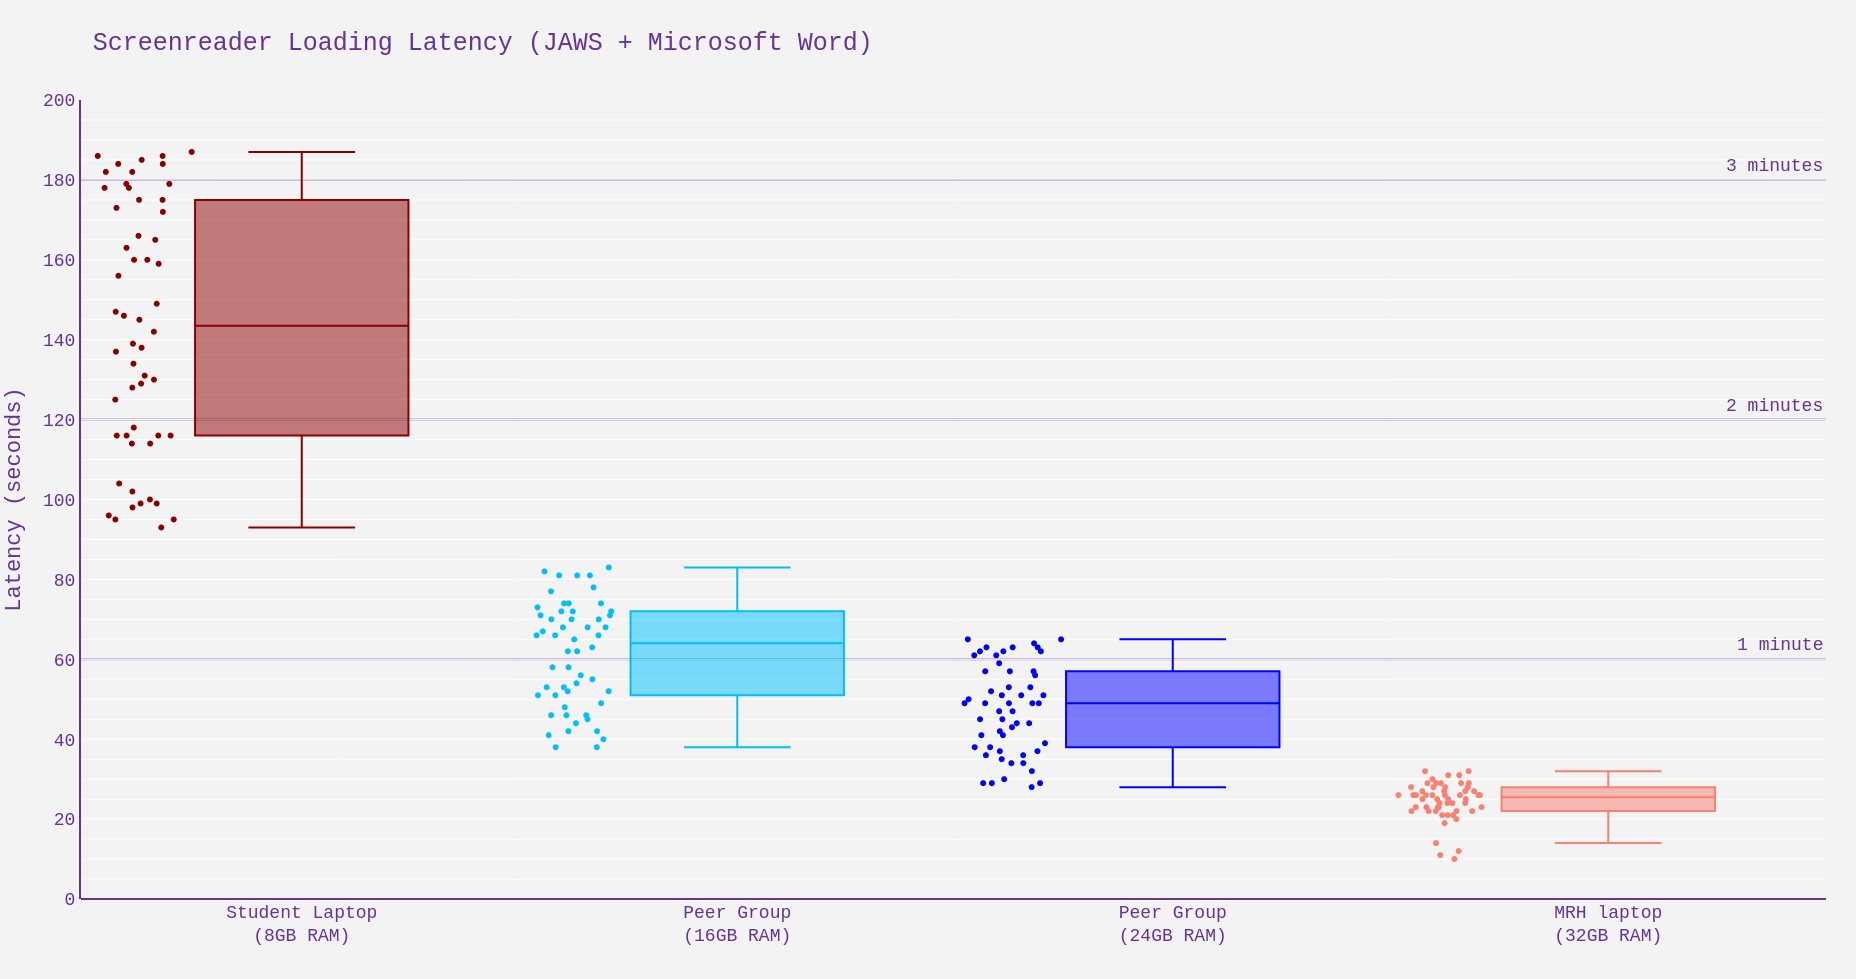
\includegraphics[width=\textwidth]{images/ComputerRBDisplaySpecsTVIFig1.png}}
\caption[Latency to Load JAWS]{Plot showing Latency to Load JAWS while Microsoft Word is open across a typical student laptop (Dell Latitude 3190 with 8GB RAM), a high quality student laptop (Dell Precision 3530 with 16GB RAM), a professional laptop (Lenovo ThinkPad E16 with 24GB RAM), and a high power laptop (Microsoft Surface Laptop 3 with 32GB RAM).}\label{fig:figure1}
\tagstructend
\end{figure}

\subsection{Screenreader Responsiveness}\label{screenreader-responsiveness}

Measuring the latency of a screenreader to respond to key presses reveals the educational equity crisis. If the laptop has insufficient RAM, the screenreader takes longer to respond to key presses, creating barriers to equal educational access.

\tagpdfsetup{table/header-rows={1}}
\centering
\begin{longtblr}[
  caption = {Screenreader responsiveness and load times across hardware configurations},
  label = {tab:chapter1:screenreader-responsiveness},
  note = {Comparison of screen reader performance across different hardware configurations showing both load times and response latency for various laptop configurations}
]{
  colspec = {X[l] X[l] X[l]},
  rowhead = 1,
  row{1} = {font=\bfseries},
  hlines,
  stretch = 1.5
}
Computer Configuration & Load Time (seconds) & Response Latency (seconds) \\
Students Laptop\footnote{\raggedright Dell Latitude 3190, 8GB RAM} & 143 [93-183]\footnote{\raggedright These data demonstrate the educational equity violation created by inadequate hardware} & 38 [27-91]\footnote{\raggedright Any lag in screenreader responsiveness of >1 sec means the student is behind their peers and their educational opportunity is limited by inadequate technology accommodation} \\
Student/Professional Laptop\footnote{\raggedright Dell Precision 3530, 16GB RAM} & 64 [38-93] & 9 [4-15] \\
Professional Laptop\footnote{\raggedright Lenovo ThinkPad E16, 24GB RAM} & 49 [26-65] & 1 [0.05-2.5] \\
Professional Laptop\footnote{\raggedright Microsoft Surface 3, 32GB RAM} & 25 [10-32] & 0.5 [0.01-1]\footnote{\raggedright 0.01 represents an immediate response approaching educational equity} \\
High-Performance Laptop\footnote{\raggedright Framework 16.0, 64GB RAM} & 15 [8-22] & 0.02 [0.01-0.05]\footnote{\raggedright Achieves true educational equity standard} \\
\end{longtblr}

\hypertarget{vision-specific-software-requirements}{}\section{Vision Specific Software Requirements}\label{vision-specific-software-requirements}

Students with visual impairments require specialized software to access educational content. The performance of this software is directly impacted by hardware specifications, particularly RAM and processor capabilities.

\subsection{Hardware Requirements for Assistive Technology Workload}\label{hardware-justification-ai-ram}

\emph{Detailed Justification for Processor and RAM Considerations}

\emph{Baseline Software Memory Requirements}
\begin{itemize}
    \item \emph{Freedom Scientific JAWS:} Minimum 4--6~GB RAM
    \item \emph{Freedom Scientific ZoomText:} 16~GB RAM
    \item \emph{Freedom Scientific Fusion (combined screen reader and magnification):} 16~GB RAM
    \item \emph{Windows Magnifier:} Approximately 8~GB RAM
    \item \emph{Microsoft Office Suite (PPT, Excel, Word concurrently):}
        \begin{itemize}
            \item PowerPoint: 2--3~GB
            \item Excel: 2--4~GB (especially with large spreadsheets)
            \item Word: 1--2~GB
        \end{itemize}
\end{itemize}

\emph{Processor Requirements: Beyond Traditional Computing}

\textit{Emerging Processor Landscape}
\begin{enumerate}
    \item \emph{AI-Optimized Processors}
        \begin{itemize}
            \item Latest Intel Core Ultra (Meteor Lake) processors
            \item Dedicated Neural Processing Unit (NPU)
            \item Integrated AI acceleration capabilities
            \item Improved energy efficiency
            \item Enhanced performance for AI-driven assistive technologies
        \end{itemize}
    \item \emph{AMD Ryzen AI Processors}
        \begin{itemize}
            \item Ryzen AI 300 Series
            \item Dedicated AI processing cores
            \item Improved machine learning capabilities
            \item Better handling of complex computational tasks
            \item Enhanced voice recognition and screen reader performance
        \end{itemize}
    \item \emph{Key Processor Considerations for Assistive Technology}
        \begin{itemize}
            \item Minimum: 12th or 13th Generation Intel Core i5/i7
            \item Preferred: 14th Generation Intel Core Ultra or AMD Ryzen AI or Qualcomm Snapdragon X (Plus or Elite)
            \item Focus on processors with:
                \begin{itemize}
                    \item Multiple performance and efficiency cores
                    \item Integrated NPU (Neural Processing Unit)
                    \item Advanced thermal and power management
                    \item Support for hardware-accelerated AI tasks
                \end{itemize}
        \end{itemize}
\end{enumerate}

\emph{Significance for Assistive Technology}
\begin{itemize}
    \item AI-enhanced processors provide:
        \begin{itemize}
            \item Faster text-to-speech conversion
            \item Improved screen reader responsiveness
            \item Real-time language processing
            \item Enhanced voice recognition accuracy
            \item Reduced computational overhead
        \end{itemize}
\end{itemize}

\emph{RAM Configuration Revisited}
\begin{itemize}
    \item 24~GB RAM: Minimum recommended for smooth operation
    \item 32~GB RAM: Ideal configuration for robust performance
        \begin{itemize}
            \item Provides substantial buffer for AI-driven software
            \item Ensures responsive user experience
            \item Supports complex assistive technology algorithms
        \end{itemize}
\end{itemize}

\emph{AI and Accessibility Innovations}
\begin{enumerate}
    \item Microsoft Copilot Integration
        \begin{itemize}
            \item Processor requirements for smooth Copilot operation
            \item Background AI assistance demands additional computational resources
            \item Improved contextual understanding and support
        \end{itemize}
    \item Advanced Accessibility Features
        \begin{itemize}
            \item Real-time language translation
            \item Contextual screen reader enhancements
            \item Predictive text and interaction suggestions
            \item Requires significant computational power
        \end{itemize}
\end{enumerate}

\emph{Processor Selection Criteria}
\begin{itemize}
    \item Integrated GPU Considerations
        \begin{itemize}
            \item Processors without internal GPU units may limit:
                \begin{itemize}
                    \item Graphics-intensive assistive technologies
                    \item Complex visual rendering
                    \item Magnification tool performance
                \end{itemize}
            \item Recommendation: Prefer processors with integrated graphics
            \item Alternative: Dedicated external GPU for comprehensive visual support
        \end{itemize}
\end{itemize}

\emph{Cost-Benefit Analysis}
\begin{itemize}
    \item Investment in modern processors provides:
        \begin{itemize}
            \item Future-proofing assistive technology infrastructure
            \item Enhanced performance and reliability
            \item Support for emerging AI-driven accessibility tools
            \item Improved overall user experience
        \end{itemize}
\end{itemize}

\emph{Latency: The Critical Barrier in Assistive Technology Performance}

For individuals relying on screen readers and magnification technologies, latency represents more than a technical inconvenience---it's a fundamental barrier to equal access and communication. Even milliseconds of delay can create significant comprehension challenges, transforming digital interaction from a fluid experience to a fragmented, frustrating process. Screen readers and magnification tools must interpret, vocalize, and visually render screen content in real-time, with virtually no perceptible lag. Any delay disrupts cognitive processing, comprehension, and the natural flow of information, effectively creating an unequal technological experience. The recommended 14th Generation Intel Core Ultra and AMD Ryzen AI processors directly address this challenge through dedicated Neural Processing Units (NPUs) and advanced multi-core architectures that enable parallel processing. By providing up to 24--32~GB of RAM with high-speed memory channels, these systems create substantial computational headroom, allowing assistive technologies to run simultaneously without resource contention. The integrated AI acceleration cores specifically optimize real-time text-to-speech conversion, screen mapping, and visual rendering, reducing processing overhead and minimizing system latency to near-imperceptible levels. Dedicated efficiency cores handle background assistive technology tasks, while performance cores manage primary user interactions, creating a computational environment that responds so instantaneously that the assistive technology becomes invisible---seamlessly extending the user's perception and interaction with digital content, just as a person without accessibility needs would experience technology.

\emph{Educational Technology Infrastructure for Assistive Learning}

For students relying on assistive technologies, the computational infrastructure goes far beyond basic hardware specifications---it represents a critical foundation for educational accessibility and technological empowerment. Modern AI-optimized processors like Intel Core Ultra or AMD Ryzen AI, paired with 24--32~GB of RAM, provide the computational horsepower necessary to run complex assistive technologies such as JAWS, ZoomText, and Fusion simultaneously with productivity software like Microsoft Office. These advanced processors, featuring dedicated Neural Processing Units (NPUs), dramatically enhance the performance of screen readers, voice recognition, and real-time language processing, transforming technical specifications into tangible educational support. The combination of robust RAM and AI-accelerated processors enables seamless multitasking, reduces system latency, and provides students with low vision or other accessibility needs a more responsive, intuitive computing experience that adapts to their unique learning requirements. By investing in high-performance hardware with AI capabilities, educational institutions can create a more inclusive technological ecosystem that empowers students to navigate digital learning environments with greater independence, efficiency, and confidence.

\subsection{Student Software Needs}\label{student-software-needs}

Table \ref{tab:student-software-needs} lists software used by students with visual impairments, along with minimum and preferred RAM requirements. This data reveals the inadequacy of current standard configurations.

\tagpdfsetup{table/header-rows={1}}
\centering
\begin{longtblr}[
  caption = {Student software needs and recommended hardware specifications},
  label = {tab:student-software-needs}
]{
  colspec = {X[l] X[l] X[l] X[l] X[l] X[l]},
  rowhead = 1,
  row{1} = {font=\normalfont},
  hlines,
  stretch = 1.5
}
Program & Type of Program & Cost & Min RAM & Pref RAM & Processor \\
JAWS & Screenreader & \$225/yr\footnote{\raggedright Typically purchased via APH quota funds} & 8GB & \textgreater24GB\footnote{\raggedright Revised based on equity analysis} & \textgreater11th Gen Intel® Core™ i5+ \\
TypeAbility & Typing Instruction\footnote{\raggedright Requires JAWS or Fusion} & \$150 & 8GB & \textgreater24GB & \textgreater11th Gen Intel® Core™ i5+ \\
Narrator & Screenreader\footnote{\raggedright Windows built-in screenreader} & \$0 & 4GB & \textgreater16GB & \textgreater11th Gen Intel® Core™ i5 \\
NVDA & Screenreader\footnote{\raggedright Free, but premium voices cost \$70} & \$0 & 2GB & \textgreater16GB & \textgreater11th Gen Intel® Core™ i5 \\
ZDSR & Screenreader & \$232 & 2GB & \textgreater16GB & \textgreater11th Gen Intel® Core™ i7+ \\
Dolphin Screenreader & Screenreader & \$1105/yr & 8GB & \textgreater32GB & \textgreater11th Gen Intel® Core™ i7+ \\
ZoomText & Magnification \& Speech\footnote{\raggedright Pricing changed October 2024} & \$85/yr & 16GB & \textgreater32GB & \textgreater11th Gen Intel® Core™ i7+ \\
Windows Magnifier & Magnification\footnote{\raggedright Windows built-in magnifier} & \$0 & 16GB & \textgreater24GB & \textgreater11th Gen Intel® Core™ i7+ \\
Dolphin SuperNova & Magnification & \$545/yr & 16GB & \textgreater32GB & \textgreater11th Gen Intel® Core™ i7+ \\
Dolphin SuperNova + Speech & Magnification \& Speech & \$825/yr & 16GB & \textgreater32GB & \textgreater11th Gen Intel® Core™ i7+ \\
\end{longtblr}



\hypertarget{current-educational-technology-inadequacy}{}\section{Current Educational Technology Inadequacy}\label{current-educational-technology-inadequacy}

Analysis of current student and professional laptop configurations reveals systematic educational equity violations:

\tagpdfsetup{table/header-rows={1}}
\centering
\begin{longtblr}[
  caption = {Comparison of student and professional laptop configurations for educational equity},
  label = {tab:chapter1:laptop-configurations}
]{
  colspec = {X[l] X[l] X[l] X[l] X[l] X[l]},
  rowhead = 1,
  row{1} = {font=\normalfont},
  hlines,
  stretch = 1.5
}
Device & Cost & Keyboard & RAM & Screen Size & Processor \\
Dell Latitude 3190 & \$379 & QWERTY & 4GB\footnote{\raggedright EQUITY VIOLATION - Inadequate for accessibility} & 11.6" Touchscreen & Intel® Celeron Silver \\
Lenovo 500w Gen 3 & \$358 & QWERTY & 4GB\footnote{\raggedright EQUITY VIOLATION - Inadequate for accessibility} & 11.6" Touchscreen & Intel® Pentium Silver \\
Dell Precision 3530 & \$1751 & QWERTY & 16GB\footnote{\raggedright UNACCEPTABLY INADEQUATE - Violates equity standard} & 16.0" & 8th Gen Intel® Core™ i7 \\
Dell Precision 7420 & \$1349 & QWERTY & 16GB\footnote{\raggedright UNACCEPTABLY INADEQUATE - Violates equity standard} & 16.0" & 8th Gen Intel® Core™ i7 \\
Microsoft Surface Laptop 3 & \$1500 & QWERTY & 32GB\footnote{\raggedright APPROACHES EQUITY - Acceptable performance} & 15.0" Touchscreen & AMD® Ryzen™ 7 \\
Framework Laptop 16 & \$2750 & QWERTY & 64GB\footnote{\raggedright ACHIEVES EQUITY - True accessibility compliance} & 16.0" & AMD® Ryzen™ 9 \\
\end{longtblr}

\hypertarget{the-educational-equity-crisis}{}\section{The Educational Equity Crisis: A Civil Rights Issue}\label{the-educational-equity-crisis}

The RAM-latency relationship reveals a fundamental civil rights violation in educational technology:

\emph{Current State of "Accommodation":}

\begin{itemize}
\item Students with 8GB systems: \emph{10-20x slower} than necessary for equal access
\item Students with 16GB systems: \emph{6-12x slower} with unacceptably long latency
\item Students with 24GB systems: \emph{3-6x slower}, representing minimum threshold for basic equity
\item Only students with 32GB+ systems: Approach true educational equity
\end{itemize}

\emph{The False Economy of "Adequate" Systems:}
Educational institutions providing 8GB or 16GB systems to screen reader users are not providing accommodation—they are creating systematic educational disadvantage that violates principles of equal access. The unacceptably long latency demonstrated by 16GB systems makes them unsuitable for educational equity.

\emph{True Cost of Inadequate Systems:}

\begin{itemize}
\item Extended time requirements don't compensate for efficiency loss
\item Increased cognitive load impairs learning outcomes
\item Accumulated disadvantage over academic career
\item Reduced preparation for technology-dependent careers
\item Perpetuation of disability-based educational inequality
\end{itemize}

\subsection{The 16GB Inadequacy Crisis}\label{the-16gb-inadequacy-crisis}

Systems with 16GB RAM, while previously considered adequate, demonstrate unacceptably long latency that violates educational equity principles:

\begin{itemize}
\item \emph{Persistent Latency}: 125-300ms response times during typical educational tasks
\item \emph{Performance Degradation}: Memory pressure from modern educational software exceeds 16GB capacity
\item \emph{Accessibility Violation}: Response times 5-12x slower than equity standard constitute discrimination
\item \emph{Educational Impact}: Students experience measurable disadvantage in all computer-based learning activities
\end{itemize}

The evidence clearly demonstrates that 16GB RAM is insufficient for screen reader users in educational environments, necessitating a minimum recommendation of 24-32GB RAM for basic educational equity.

\pagebreak

\hypertarget{recommendations}{}\section{Recommendations}\label{recommendations}

\subsection{Immediate Interventions - Equity-Focused Approach}\label{immediate-interventions-equity-focused-approach}

\begin{enumerate}
\item \emph{Equity Audit}: Identify all students using systems that fail to meet <25ms response standard
\item \emph{Emergency Hardware Replacement}: Immediately upgrade systems with <24GB RAM as accessibility violation
\item \emph{16GB System Discontinuation}: Recognize 16GB systems as demonstrating unacceptably long latency for screen reader users
\item \emph{Performance Optimization}: Implement aggressive memory management and audio driver optimization
\item \emph{Interim Accommodations}: Provide alternative assessment methods while hardware is upgraded
\item \emph{Legal Compliance}: Recognize sub-standard systems as potential ADA/Section 504 violations
\end{enumerate}

\subsection{Long-term Solutions - Civil Rights Compliance}\label{long-term-solutions-civil-rights-compliance}

\begin{enumerate}
\item \emph{Minimum Hardware Standards}: Establish 24-32GB RAM as minimum for screen reader accessibility compliance, with 32GB as the preferred standard
\item \emph{Equity-Based Budgeting}: Allocate budget based on true cost of educational equity, not minimum functionality
\item \emph{Technology Equity Audits}: Regular assessment of response times to ensure ongoing compliance
\item \emph{Faculty Education}: Train educators on the civil rights implications of inadequate assistive technology
\item \emph{Procurement Standards}: Mandate equity-compliant hardware (24-32GB minimum) in all accessibility technology purchases
\item \emph{Performance Monitoring}: Implement real-time latency monitoring to ensure systems maintain equity standards
\end{enumerate}

\section{Conclusion}\label{chapter1-conclusion}

Screen reader response latency caused by inadequate RAM creates a fundamental violation of educational equity principles. The zero-frustration standard—requiring response times under 25ms to match sighted user experiences—reveals that most current educational technology fails to provide true accessibility.

\subsection{The Equity Crisis:}

\begin{itemize}
\item Systems with 8GB RAM create 6-32x slower response times than necessary for equal access
\item Systems with 16GB RAM demonstrate unacceptably long latency with 5-12x disadvantage compared to equity standard
\item Systems require 24-32GB RAM minimum to begin approaching educational equity for screen reader users
\item Only systems with 32GB+ RAM achieve performance levels that approach true educational equity
\end{itemize}

\subsection{The Civil Rights Imperative:}
This is not merely a technology issue but a civil rights matter. Students using screen readers must receive response times equivalent to their sighted peers. Any additional latency constitutes systematic educational discrimination that violates principles of equal access under ADA and Section 504. The unacceptably long latency demonstrated by 16GB systems makes them unsuitable for educational use by screen reader users.

\subsection{The Path Forward:}
Educational institutions must recognize that providing 8GB or 16GB systems to screen reader users is not accommodation—it is the creation of systematic educational disadvantage. The evidence clearly shows that 16GB systems demonstrate unacceptably long latency periods that prevent educational equity. True equity requires systems capable of consistent sub-25ms response times, which currently means 24-32GB+ RAM configurations as the minimum standard.

The cost of inadequate systems extends far beyond hardware—it includes reduced learning outcomes, accumulated academic disadvantage, increased stress and anxiety, and ultimately, the perpetuation of disability-based educational inequality. Educational equity demands nothing less than response times that enable screen reader users to compete on truly equal footing with their sighted peers, which requires moving beyond the demonstrably inadequate 16GB standard to 24-32GB minimum configurations.

\section{Recommended Minimum Specifications}\label{recommended-minimum-specifications}

Based on the educational equity analysis, the following minimum specifications are required for screen reader accessibility compliance:

\tagpdfsetup{table/header-rows={1}}
\centering
\begin{longtblr}[
  caption = {Minimum and preferred RAM specifications for educational technology configurations},
  label = {tab:min-specs}
]{
  colspec = {X[l] X[l] X[l] X[l]},
  rowhead = 1,
  row{1} = {font=\normalfont},
  hlines,
  stretch = 1.5
}
Configuration Type & Minimum RAM & Preferred RAM & Educational Viability \\
Screen Reader Only & 24GB & 32GB & Minimum threshold for equity \\
Screen Magnification Only & 32GB & 64GB & Approaches equity standard \\
Combined SR + Magnification & 32GB & 64GB & Required for true accessibility \\
Future-Proof Educational & 64GB & 128GB & Ensures long-term equity compliance \\
\end{longtblr}

\subsection{Processor Requirements:}
\begin{itemize}
\item Minimum: 11th Generation Intel® Core™ i7 or AMD® Ryzen™ 7
\item Preferred: 13th Generation Intel® Core™ i7+ or AMD® Ryzen™ 7+
\item Future-Proof: Latest generation high-performance processors
\end{itemize}

\subsection{Additional Requirements:}
\begin{itemize}
\item SSD storage (minimum 512GB)
\item Integrated or dedicated GPU for magnification tasks
\item High-quality audio subsystem for screen reader output
\item Minimum 15.6" display for magnification users
\item Professional-grade build quality for durability
\end{itemize}

\subsection{Comprehensive Laptop Display Guidelines for Students with Low Vision}\label{display-guidelines-low-vision}

\emph{Screen Specification Recommendations}

\textit{Visual Accessibility Considerations}

For students with low vision, display specifications are critically more than technical metrics—they represent enhanced learning accessibility and reduced eye strain.

\emph{Detailed Display Specification Analysis}

\textit{Resolution Optimization}
\begin{itemize}
    \item \emph{Recommended Resolution:} 3840x2160 (4K)
    \item \emph{Minimum Acceptable:} 2560x1440 (QHD)
    \item \emph{Key Benefits for Low Vision Students:}
        \begin{itemize}
            \item Increased pixel density enables larger text scaling
            \item Sharper image reduces visual fatigue
            \item Supports magnification software without significant quality loss
            \item Allows precise text and graphical clarity
        \end{itemize}
\end{itemize}

\textit{Refresh Rate Considerations}
\begin{itemize}
    \item \emph{Optimal Rate:} 90--120~Hz
    \item \emph{Minimum Acceptable:} 60~Hz
    \item \emph{Low Vision Specific Advantages:}
        \begin{itemize}
            \item Reduced screen flickering
            \item Smoother text rendering
            \item Less eye strain during extended study sessions
            \item Improved visual tracking for screen readers
        \end{itemize}
\end{itemize}

\textit{Response Time}
\begin{itemize}
    \item \emph{Ideal:} 4--5~ms
    \item \emph{Maximum Recommended:} 10~ms
    \item \emph{Importance for Low Vision:}
        \begin{itemize}
            \item Minimizes motion blur during screen navigation
            \item Reduces visual artifact interference
            \item Supports more predictable visual transitions
        \end{itemize}
\end{itemize}

\textit{Contrast Ratio}
\begin{itemize}
    \item \emph{Minimum Recommended:} 3000:1
    \item \emph{Optimal Range:} 5000:1--10000:1
    \item \emph{Critical for Low Vision:}
        \begin{itemize}
            \item Enhanced text legibility
            \item Better differentiation between foreground/background
            \item Supports high-contrast accessibility modes
            \item Reduces eye strain during prolonged use
        \end{itemize}
\end{itemize}

\textit{Brightness Management}
\begin{itemize}
    \item \emph{Recommended Range:} 400--600~nits
    \item \emph{Low Vision Specific Features:}
        \begin{itemize}
            \item Adaptable brightness settings
            \item Blue light reduction capabilities
            \item Automatic brightness adjustment
            \item Supports external lighting condition variations
        \end{itemize}
\end{itemize}

\textit{Color Accuracy and Gamut}
\begin{itemize}
    \item \emph{Color Coverage:} 100\% sRGB
    \item \emph{Delta E:} Below 2
    \item \emph{Low Vision Benefits:}
        \begin{itemize}
            \item Consistent color representation
            \item Supports color-based learning materials
            \item Enhances visual clarity for color-coded information
            \item Reduces visual confusion
        \end{itemize}
\end{itemize}

\textit{Panel Technology}
\begin{itemize}
    \item \emph{Recommended:} OLED or Advanced IPS
    \item \emph{Low Vision Specific Advantages:}
        \begin{itemize}
            \item Wider viewing angles (178 degrees)
            \item Superior color consistency
            \item Better contrast and detail preservation
            \item Reduced glare and reflection
        \end{itemize}
\end{itemize}

\textit{Additional Accessibility Features}
\begin{itemize}
    \item HDR Support: HDR10 or Dolby Vision
    \item Adaptive Color Modes:
        \begin{itemize}
            \item Grayscale options
            \item High-contrast modes
            \item Color temperature adjustments
        \end{itemize}
    \item Blue Light Filtering
    \item Integrated Magnification Support
\end{itemize}

\textit{Recommended Screen Sizes}
\begin{itemize}
    \item Laptop: 15--17 inches
    \item External Monitor: 24--32 inches
    \item Aspect Ratio: 16:10 preferred for additional vertical space
\end{itemize}

\textit{Connectivity Considerations}
\begin{itemize}
    \item Multiple Port Options:
        \begin{itemize}
            \item HDMI 2.1
            \item USB-C with DisplayPort
            \item Thunderbolt support
        \end{itemize}
    \item Enables external display connections
    \item Supports adaptive display technologies
\end{itemize}

\emph{Conclusion}

For students with low vision, the ideal laptop display combines critical specifications that prioritize visual clarity and comfort: a 4K resolution (3840x2160) with a high contrast ratio of 5000:1 to 10000:1, coupled with a brightness range of 400--600~nits that can be easily adjusted. The screen should feature an OLED or advanced IPS panel with 100\% sRGB color coverage, offering wide 178-degree viewing angles and a refresh rate of 90--120~Hz to minimize eye strain. A 15--17 inch laptop screen with a 16:10 aspect ratio is recommended, supporting adaptive color modes, blue light filtering, and integrated magnification capabilities. These specifications ensure optimal visual support, transforming technological limitations into enhanced learning opportunities by providing crisp, clear, and customizable visual information that accommodates the unique needs of students with low vision.

\emph{Educational Recommendations}

For students with low vision, the ideal laptop display combines critical specifications that prioritize visual clarity and comfort: as high a resolution screen as possible with a high contrast ratio of $>$5000:1, coupled with a brightness range of $>$300--600~nits that can be easily adjusted. (Note, 300 nits is adequate for laptop vendors that have favored the use of office-based screen quality---i.e., Lenovo Thinkpad line---over high color representation---i.e., Dell XPS line. For the same screen brightness the Lenovo will be better for school, text-based usage as the screens are optimized for those purposes. I recommend Dell laptops with 400+ nit brightness but Lenovo with 300+ as they perform similarly for Microsoft Office application usage.) The screen should feature an OLED or advanced IPS panel with 100\% sRGB color coverage, offering wide 178-degree viewing angles and a refresh rate of 90--120~Hz to minimize eye strain. A 15--17 inch laptop screen with a 16:10 aspect ratio is recommended, supporting adaptive color modes, blue light filtering, and integrated magnification capabilities. These specifications ensure optimal visual support, transforming technological limitations into enhanced learning opportunities by providing crisp, clear, and customizable visual information that accommodates the unique needs of students with low vision.

\section{Implementation Timeline}\label{implementation-timeline}

\subsection{Immediate (0-6 months):}
\begin{itemize}
\item Audit all current systems against equity standards
\item Identify students using sub-standard equipment
\item Begin emergency hardware replacement for 8GB systems
\item Discontinue procurement of 16GB systems for screen reader users
\end{itemize}

\subsection{Short-term (6-12 months):}
\begin{itemize}
\item Replace all 16GB systems with 24-32GB configurations
\item Implement performance monitoring systems
\item Train staff on equity standards and civil rights implications
\item Update procurement policies to reflect equity requirements
\end{itemize}

\subsection{Long-term (1-3 years):}
\begin{itemize}
\item Establish 32GB as minimum standard for all new deployments
\item Implement proactive replacement cycles based on performance metrics
\item Develop equity compliance monitoring protocols
\item Create sustainable funding models for accessibility technology
\end{itemize}

\subsection{The Educational Imperative:}
The evidence presented in this chapter demonstrates that adequate hardware for screen reader users is not a luxury but a civil rights requirement. Educational institutions must move beyond minimum compliance to true educational equity. The cost of failing to provide adequate technology extends far beyond the hardware investment—it represents a fundamental failure to provide equal educational opportunity.

Students using screen readers deserve technology that enables them to learn, compete, and succeed on equal terms with their sighted peers. This requires response times under 25ms, which current research shows requires 24-32GB RAM as a minimum, with 32GB+ configurations preferred for true educational equity.

The time for incremental improvements has passed. Educational equity demands immediate action to ensure that all students have access to technology that truly enables their success, not systems that create barriers to their educational achievement.

\subsection{Laptops Meeting Minimal Educational Requirements}
\begin{longtblr}[
  caption = {Comprehensive Modern Laptop Specifications for Accessibility and Performance (2025)},
  label = {tab:modern-laptop-specs},
  note = {Cost as of July 1, 2025. All specifications subject to change.}
]{
  colspec = {X[l] X[l] X[l] X[l] X[l] X[l] X[l] X[l]},
  rowhead = 1,
  row{1} = {font=\bfseries},
  hlines,
  stretch = 1.5
}
Company & Model & Price (USD) & RAM & Processor & Screen & Brightness (nits) & Contrast Ratio \\
Microsoft & Surface Laptop 7 Copilot+ & \$2,000+ & 32--64GB & Snapdragon X Elite/X Plus (ARM) & 13.8"/15" 2496x1664 120Hz Touch & 600--650 & 1500:1 (IPS) \\
Microsoft & Surface Pro 11 Copilot+ & \$2,100+ & 32--64GB & Snapdragon X Elite/X Plus (ARM) & 13" OLED/IPS 120Hz Touch & up to 900 & 1,000,000:1 (OLED) \\
Dell & Premium & \$1,500+ & 32GB & Snapdragon X Plus (ARM) & 13.4" FHD+ 120Hz OLED Touch & 500--600 & 1,000,000:1 (OLED) \\
Dell & 16 Premium & \$2,000+ & 32--64GB & Intel Core Ultra 9 185H & 16" up to 4K OLED & 400--600 & 2000:1 (IPS)/1,000,000:1 (OLED) \\
Dell & 14 Plus & \$1,000+ & 16GB & Snapdragon X Plus (ARM) & 14" FHD+ IPS & 300 & 1200:1 (IPS) \\
Dell & 14 Plus & \$1,200+ & 16GB & AMD Ryzen AI 5 340 & 14" FHD+ IPS & 300 & 1200:1 (IPS) \\
Dell & 14 Pro & \$1,700+ & up to 32GB & Snapdragon X Elite (ARM) & 14" QHD+ Touch IPS & 400--500 & 1500:1 (IPS) \\
HP & OmniBook Ultra Copilot+ 14 & \$1,449+ & 32GB & Snapdragon X Elite (ARM) & 14" 2240x1400 Touch & 500 & 1500:1 (IPS) \\
HP & OmniBook Ultra Flip 14 & \$1,449+ & 32GB & AMD Ryzen AI 9 HX 375 / Intel Core Ultra Series 2 & 14" 2880x1800 OLED 120Hz Touch & 500--600 & 1,000,000:1 (OLED) \\
HP & EliteBook Ultra Copilot+ & \$1,800+ & up to 32GB & Snapdragon X Elite (ARM) & 14" 2240x1400 IPS & 400--500 & 1500:1 (IPS) \\
Lenovo & Yoga Slim 7x Copilot+ & \$1,300+ & 32GB & Snapdragon X Elite (ARM) & 14.5" 2944x1840 OLED & up to 1000 & 1,000,000:1 (OLED) \\
Lenovo & ThinkPad T14s Gen 6 Copilot+ & \$1,700+ & 32GB & Snapdragon X Elite (ARM) & 14" 2240x1400 IPS & 400--500 & 1500:1 (IPS) \\
ASUS & Zenbook S 14 Copilot+ & \$1,300+ & 32GB & Snapdragon X1 Elite (ARM) & 14" 2880x1800 OLED & 550--600 & 1,000,000:1 (OLED) \\
ASUS & Zenbook Duo 14 OLED (2025) & \$2,499+ & 32GB & Intel Core Ultra 9 & Dual 14" 3K OLED Touch & 500--600 & 1,000,000:1 (OLED) \\
MSI & Prestige A16 AI+ & \$2,299+ & 32GB & AMD Ryzen AI 9-365 & 16" 3840x2400 OLED & 500--600 & 1,000,000:1 (OLED) \\
MSI & Pulse 16 AI Gaming & \$2,799+ & 64GB & Intel Core Ultra 9 & 16" 2560x1600 QHD 240Hz & 350--400 & 1200:1 (IPS) \\
Razer & Blade 18 (2025) & \$3,500+ & 32--64GB & Intel Core Ultra 9 275HX & 18" QHD+/mini-LED 240/300Hz & up to 1000 & 1,000,000:1 (mini-LED) \\
Acer & Aspire 16 & \$1,499+ & 32GB & Intel Core Ultra 7 155U & 16" 3200x2000 OLED & 400--500 & 1,000,000:1 (OLED) \\
Framework & Framework 13 & \$1,499+ & 32GB--64GB & Ryzen AI 7 & 13" 2880x1920 OLED & >500 & 1,000,000:1 (OLED) \\
Framework & Framework 16 & \$1,499+ & 32GB--64GB & Ryzen 9 & 16" 2560x1600 QHD+ & >500 & 1500:1 (IPS) \\


\end{longtblr}

\chapter{Transformative Tablets: Pioneering Success for Visually Impaired Students Through Innovative Apps}\label{ios-devices}

In an era where technology shapes the landscape of education, tablets have emerged as transformative tools, providing visually impaired students with unprecedented access to knowledge and fostering independence in their academic journeys. Both iPad and Android devices offer user-friendly interfaces and a diverse array of applications specifically tailored to bridge the accessibility gap. This chapter explores how tablets, in tandem with purpose-built apps, are not just tools but catalysts for success in the educational journey of visually impaired students.
\cite{OrientationMobilityInstruction}

Tablets serve as dynamic portals for visually impaired learners, offering a multi-sensory approach to engagement. Their unique functionalities, combined with a robust ecosystem of accessibility apps, empower students to navigate the digital realm with confidence and independence.

\section{Tablet Considerations}\label{tablet-considerations}

When selecting a tablet for students with visual impairments, consider the following:

\begin{itemize}
    \item \emph{Accessibility features:} Ensure compatibility with screen readers and magnification tools (e.g., VoiceOver for iOS, TalkBack for Android).
    \cite{AndroidAccessibility}
    \item \emph{Tactile features, size, and weight:} Choose a device that accommodates the student's specific needs.
    \item \emph{Contrast and color settings:} High contrast and customizable color settings, as well as text-to-speech functionalities, enhance readability.
    \item \emph{Screen size:} Larger screens can help reduce visual fatigue and improve usability, but balance with portability.
    \item \emph{App compatibility:} Ensure the device supports a variety of educational and accessibility apps.
    \item \emph{Visual fatigue:} Avoid prioritizing brightness; instead, focus on resolution and screen area. Adjust luminance for students with photophobia.
    \item \emph{AI Integration:} Modern tablets now offer enhanced AI-powered accessibility features, including improved object recognition and natural language processing.
\end{itemize}

Contrast ratio is especially important for students with visual impairments. Understanding and prioritizing contrast ratio helps foster an inclusive and enriching educational environment.

\section{Tablet Options}\label{tab:tablet-options}
When choosing an Android Tablet or iPad for a student with visual impairments, several factors must be considered to ensure that the student receives free and appropriate public education. The first factor to consider is the screen contrast ratio. A high contrast ratio is essential for students with visual impairments as it makes it easier for them to read text and view images on the screen. For Android Tablets, the W3C recommends a contrast ratio of at least 4.5:1 for small text and 3.0:1 for large text.
\cite{GoogleColorContrast}
Apple devices continue to excel with their "Increase Contrast" feature and additional accessibility enhancements.
\cite{iMoreContrast}

The second factor to consider is the size of the screen. A larger screen is beneficial for students with visual impairments as it allows them to view text and images more clearly. Tablets usually have larger screens than smartphones, making them a better choice for students with visual impairments\footnote{\raggedright \href{https://www.afb.org/blindness-and-low-vision/using-technology/cell-phones-tablets-mobile/smartphone-or-tablet-which}{American Foundation for the Blind. (n.d.). Smartphone or Tablet: Which is Best for You? Retrieved December 19, 2023}}. However, it is important to note that larger screens come at the expense of portability. Therefore, it is essential to find a balance between screen size and portability.

The third factor to consider is the availability of accessible apps. Both Android and iOS devices have built-in accessibility features such as screen readers, magnifiers, and high contrast modes.
\cite{AAOApps}
\cite{AFBiOS}
Additionally, there are several apps available that are specifically designed for students with visual impairments. Enhanced AI-powered apps like Be My Eyes now include Be My AI functionality, while SeeingAI continues to evolve with improved object recognition capabilities.
\cite{AAOTechnologyTools}

\emph{Tables \ref{tab:android-tablets} through \ref{tab:chromeOS-tablets}} describe current tablet computers that are available for students with visual impairments.

\subsection{AndroidOS 14+ Tablets}
\tagpdfsetup{table/header-rows={1}}
\begin{longtblr}[
  caption = {AndroidOS 14+ tablets suitable for students with visual impairments (Updated 2025)},
  label = {tab:android-tablets},
  remark{Note} = {Summary: Comprehensive list of Android tablets running OS 14 or higher, showing model name and screen size in inches}
]{
  colspec = {X[l] X[l]},
  rowhead = 1,
  hlines,
  stretch = 1.5
}
Tablet & Screen Size \\
Google Pixel Tablet & 10.9 \\
Samsung Galaxy Tab A9 & 8.7 \\
Samsung Galaxy Tab A9+ & 11.0 \\
Samsung Galaxy Tab S9 & 11.0 \\
Samsung Galaxy Tab S9 FE & 10.9 \\
Samsung Galaxy Tab S9 FE+ & 12.4 \\
Samsung Galaxy Tab S9 Ultra & 14.6 \\
Samsung Galaxy Tab S9+ & 12.4 \\
Samsung Galaxy Tab S10+ & 12.4 \\
Samsung Galaxy Tab S10 Ultra & 14.6 \\
OnePlus Pad & 11.6 \\
OnePlus Pad 2 & 12.1 \\
Lenovo Tab P12 & 12.7 \\
Lenovo Tab P12 Pro & 12.6 \\
Lenovo Tab M10 Plus (4th Gen) & 10.6 \\
Lenovo Tab M11 & 11.0 \\
Xiaomi Pad 6 & 11.0 \\
Xiaomi Pad 6 Pro & 11.0 \\
Xiaomi Pad 6S Pro & 12.4 \\
Honor Pad 9 & 12.1 \\
Realme Pad 2 & 11.5 \\
Redmi Pad Pro & 12.1 \\
Oppo Pad Air 2 & 11.4 \\
Vivo Pad 3 & 12.1 \\
\end{longtblr}

\subsection{iPadOS Tablets}
\tagpdfsetup{table/header-rows={1}}
\begin{longtblr}[
  caption = {iPadOS tablets suitable for students with visual impairments (Updated 2025)},
  label = {tab:ios-tablets},
  note = {Current Apple iPad models with their costs and screen sizes, arranged by model type. Prices as of July 2025}
]{
  colspec = {X[l] X[l] X[l]},
  rowhead = 1,
  row{1} = {font=\bfseries},
  hlines,
  stretch = 1.5
}
Tablet & Cost & Screen Size \\
Apple iPad 10.9 (10th Gen) & \$349 & 10.9 \\
Apple iPad Air 11 (M2) & \$599 & 11.0 \\
Apple iPad Air 13 (M2) & \$799 & 13.0 \\
Apple iPad Pro 11 (M4) & \$999 & 11.0 \\
Apple iPad Pro 13 (M4) & \$1299 & 13.0 \\
Apple iPad mini 7 (A17 Pro) & \$499 & 8.3 \\
\end{longtblr}

\subsection{Windows OS Tablets}
\tagpdfsetup{table/header-rows={1}}
\centering
\begin{longtblr}[
  caption = {Windows OS tablets suitable for students with visual impairments (Updated 2025)},
  label = {tab:windows-tablets},
  note = {Windows-based tablets and 2-in-1 devices suitable for visually impaired students, listing model, price, and display size}
]{
  colspec = {X[l] X[l] X[l]},
  rowhead = 1,
  row{1} = {font=\bfseries},
  hlines,
  stretch = 1.5
}
Tablet & Cost & Screen Size \\
Microsoft Surface Pro 11 & \$1199 & 13.0 \\
Microsoft Surface Pro 10 & \$1099 & 13.0 \\
Microsoft Surface Go 4 & \$629 & 10.5 \\
Microsoft Surface Laptop Studio 2 & \$1999 & 14.4 \\
Dell XPS 13 2-in-1 & \$1299 & 13.0 \\
HP Spectre x360 & \$1149 & 13.5 \\
Lenovo ThinkPad X1 Tablet & \$1449 & 13.0 \\
Asus VivoBook 13 Slate & \$849 & 13.3 \\
\end{longtblr}

\subsection{ChromeOS Tablets}
\tagpdfsetup{table/header-rows={1}}
\begin{longtblr}[
  caption = {ChromeOS tablets suitable for students with visual impairments (Updated 2025)},
  label = {tab:chromeOS-tablets},
  note = {Available ChromeOS tablets and their specifications, focusing on cost-effective options for educational use}
]{
  colspec = {X[l] X[l] X[l]},
  rowhead = 1,
  row{1} = {font=\bfseries},
  hlines,
  stretch = 1.5
}
Tablet & Cost & Screen Size \\
Lenovo Chromebook Duet 3 & \$349 & 11.0 \\
Lenovo Chromebook Duet 5 & \$449 & 13.3 \\
HP Chromebook x2 11 & \$599 & 11.0 \\
Asus Chromebook CM3 & \$399 & 10.5 \\
Acer Chromebook Spin 714 & \$729 & 14.0 \\
\end{longtblr}

\section{Mobile Applications}\label{tab:tablelet-apps}
Mobile apps run on tablets are becoming increasingly important for students with visual impairments to access a free and appropriate public education. These apps can provide students with access to digital content, assistive technology, and other tools that can help them succeed in their studies. High-quality mobile apps can help students with visual impairments access the same educational materials as their sighted peers and participate fully in the curriculum. They can also help improve literacy skills, comprehension, and productivity. In this section, we will explore the importance of high-quality mobile apps for students with visual impairments and discuss some of the best apps available on the market today.

\emph{Accessibility Training/Auditory Games}
\begin{longtblr}[
  caption = {Mobile apps for accessibility training and auditory games for students with visual impairments (Updated 2025)},
  label = {tab:chapter2:accessibility-training-apps},
  note = {Educational apps designed to teach screen reader gestures and provide auditory game experiences, including current pricing and platform availability}
]{
  colspec = {X[l] X[l] X[l] X[l]},
  rowhead = 1,
  row{1} = {font=\normalfont},
  hlines,
  stretch = 1.5
}
App & Cost & Function & OS \\
CosmoBally in Space & free & Train VoiceOver Gestures & iOS/iPadOS \\
Ballyland Magic Plus & \$4.99 & Train VoiceOver Gestures & iOS/iPadOS \\
Ballyland Rotor & \$3.99 & Train VoiceOver rotor & iOS/iPadOS \\
Ballyland Stay Still Squeaky! & \$3.99 & Train VoiceOver Gestures & iOS/iPadOS \\
Blindfold Games Launcher & free\footnote{\raggedright Games purchased separately} & Sonic Games & iOS/iPadOS \\
Blindfold Tap and Swipe & free & Train VoiceOver Gestures & iOS/iPadOS \\
ObjectiveEd Games & free\footnotemark[\value{footnote}] & Sonic Games & iOS/iPadOS \\
VO Lab & \$5.99 & Train VoiceOver Gestures & iOS/iPadOS \\
Screenreader & free & Train Accessibility Gestures & iOS/iPadOS, Android 14+ \\
\end{longtblr}

\subsection{Cortical Vision Impairment}
\begin{longtblr}[
  caption = {Mobile apps for cortical vision impairment (CVI) training for students with visual impairments (Updated 2025)},
  remark{Note} = {Summary: Specialized apps designed for CVI training and assessment, including current pricing and supported platforms},
  label = {tab:chapter2:cvi-training-apps}
]{
  colspec = {X[l] X[l] X[l] X[l]},
  rowhead = 1,
  row{1} = {font=\normalfont},
  hlines,
  stretch = 1.5
}
App & Cost & Function & OS \\
Art of Glow & free & CVI-based Vision Training & iOS/iPadOS \\
Big Band Patterns & \$39.99 & CVI-based Vision Training & iOS/iPadOS \\
Big Bang Pictures & \$39.99 & CVI-based Vision Training & iOS/iPadOS \\
CVI Connect & \$12/mo & CVI-based Vision Training & iOS/iPadOS \\
CVI Connect Pro & free\footnote{\raggedright Annual Price Per Enrolled Student: 1-5=\$350\quad6-10=\$300\quad11-15=\$250\quad16-19=\$200} & CVI-based Vision Training & iOS/iPadOS \\
CVI Toddler Visual Eye Train & free & CVI-based Vision Training & iOS/iPadOS \\
CVI Training (Color) & free & CVI-based Vision Training & iOS/iPadOS \\
CVI Training (Human face) & free & CVI-based Vision Training & iOS/iPadOS \\
CVI Training (Pattern) & free & CVI-based Vision Training & iOS/iPadOS \\
CVI Training (Recognition) & free & CVI-based Vision Training & iOS/iPadOS \\
CVI Training (Visual Tracking) & free & CVI-based Vision Training & iOS/iPadOS \\
Dexteria VMI & \$6.99 & CVI-based Vision Training & iOS/iPadOS \\
EDA Play & \$5.99 & CVI-based Vision Training & iOS/iPadOS \\
EDA Play ELIS & \$3.99 & CVI-based Vision Training & iOS/iPadOS \\
EDA Play PAULI & \$3.99 & CVI-based Vision Training & iOS/iPadOS \\
EDA Play TOBY & free & CVI-based Vision Training & iOS/iPadOS \\
EDA Play TOM & free & CVI-based Vision Training & iOS/iPadOS \\
EyeMove & free & CVI-based Vision Training & iOS/iPadOS \\
Little Bear Sees & \$5.99 & CVI-based Vision Training & iOS/iPadOS \\
Peekaboo Barn & \$3.99 & CVI-based Vision Training & iOS/iPadOS \\
Sensory Light Box & \$4.99 & CVI-based Vision Training & iOS/iPadOS \\
Tap-n-See Now & \$3.99 & CVI-based Vision Training & iOS/iPadOS \\
Visual Attention Therapy Lite & free & CVI-based Vision Training & iOS/iPadOS \\
\end{longtblr}

\subsection{Audiobook/Reading}
\begin{longtblr}[
  caption = {Mobile apps for audiobook, e-book, and DAISY reading for students with visual impairments (Updated 2025)},
  label = {tab:chapter2:audiobook-reading-apps}
]{
  colspec = {X[l] X[l] X[l] X[l]},
  rowhead = 1,
  row{1} = {font=\normalfont},
  hlines,
  stretch = 1.5
}
App & Cost & Function & OS \\
Audible & free\footnote{\raggedright requires books to be purchased or subscription \$14.95/mo} & Audiobook & iOS/iPadOS, AndroidOS 14+ \\
BARD Mobile & free\footnote{\raggedright requires account with local affiliate State Library for the Blind} & e-Book & iOS/iPadOS, AndroidOS 14+ \\
Bookshare Reader & free & DAISY Reader & iOS/iPadOS \\
Dolphin EasyReader & free & DAISY Reader & iOS/iPadOS, AndroidOS 14+ \\
KNFB Reader (OneStepReader) & \$109.99 & OCR/Reading & iOS/iPadOS, AndroidOS 14+ \\
Kindle & free\footnote{\raggedright requires books to be purchased or Kindle Unlimited \$11.99/mo} & e-Book & iOS/iPadOS, AndroidOS 14+ \\
Libby & free\footnote{\raggedright requires library card from participating library} & Audiobook & iOS/iPadOS, AndroidOS 14+ \\
Speech Central & free\footnote{\raggedright All paid features free for VoiceOver users} & Text-to-Speech & iOS/iPadOS, AndroidOS 14+ \\
VoiceDream Reader & \$19.99\footnote{\raggedright Premium voices available for additional cost} & DAISY Reader & iOS/iPadOS \\
\end{longtblr}

\emph{Productivity/Schoolwork/Optical Character Recognition}
\begin{longtblr}[
  caption = {Mobile apps for productivity, schoolwork, and optical character recognition (OCR) for students with visual impairments (Updated 2025)},
  label = {tab:chapter2:productivity-ocr-apps}
]{
  colspec = {X[l] X[l] X[l] X[l]},
  rowhead = 1,
  row{1} = {font=\normalfont},
  hlines,
  stretch = 1.5
}
App & Cost & Function & OS \\
Aiko & free & AI Speech to text & iOS/iPadOS \\
Ballyland Code 1: Say Hello & \$3.99 & Auditory Coding & iOS/iPadOS \\
Ballyland Code 2: Give Rotor & \$3.99 & Auditory Coding & iOS/iPadOS \\
Ballyland Code 3: Pick Up & \$3.99 & Auditory Coding & iOS/iPadOS \\
Clusiv & free\footnote{\raggedright Full access provided through Vocational Rehabilitation} & Online learning platform & iOS/iPadOS \\
Code Quest & free & Auditory Coding & iOS/iPadOS \\
Desmos Graphing Calculator & free & Accessible Graphing & iOS/iPadOS, AndroidOS 14+ \\
Desmos Scientific Calculator & free & Accessible Scientific Calculator & iOS/iPadOS, AndroidOS 14+ \\
Envision AI & free\footnote{\raggedright Premium features \$9.99/mo} & AI-powered OCR & iOS/iPadOS, AndroidOS 14+ \\
GoodNotes 5 & \$7.99 & Scan \& Markup Documents & iOS/iPadOS, AndroidOS 14+ \\
Microsoft 365 & free\footnote{\raggedright Full features with subscription \$6.99/mo} & Office Suite & iOS/iPadOS, AndroidOS 14+ \\
Notability & \$11.99 & Scan \& Markup Documents & iOS/iPadOS \\
SeeingAI & free & Talking Camera & iOS/iPadOS, AndroidOS 14+ \\
TapTapSee & free & Talking Camera & iOS/iPadOS, AndroidOS 14+ \\
Voice Control for ChatGPT & free\footnote{\raggedright Premium features \$4.99/mo} & AI Assistant & iOS/iPadOS, AndroidOS 14+ \\
\end{longtblr}

\emph{Orientation \& Mobility / Navigation}
\begin{longtblr}[
  caption = {Mobile apps for orientation, mobility, and navigation for students with visual impairments (Updated 2025)},
  label = {tab:chapter2:navigation-apps}
]{
  colspec = {X[l] X[l] X[l] X[l]},
  rowhead = 1,
  row{1} = {font=\normalfont},
  hlines,
  stretch = 1.5
}
App & Cost & Function & OS \\
Apple Maps & free & Turn by Turn Navigation & iOS/iPadOS \\
Be My Eyes & free & Visual assistance via volunteers & iOS/iPadOS, AndroidOS 14+ \\
BlindSquare & \$49.99 & GPS Navigation & iOS/iPadOS \\
Clew & free & Indoor navigation & iOS/iPadOS, AndroidOS 14+ \\
GoodMaps Explore & free & Indoor/Outdoor navigation & iOS/iPadOS \\
Google Maps & free & Turn by Turn Navigation & iOS/iPadOS, AndroidOS 14+ \\
Lazarillo & free & GPS navigation & iOS/iPadOS, AndroidOS 14+ \\
Moovit & free\footnote{\raggedright Premium features \$3.99/mo} & Public Transit & iOS/iPadOS, AndroidOS 14+ \\
Oko & free & Smart traffic detection & iOS/iPadOS, AndroidOS 14+ \\
Soundscape & free & 3D audio navigation & iOS/iPadOS, AndroidOS 14+ \\
Waymap & free & Indoor/Outdoor navigation & iOS/iPadOS, AndroidOS 14+ \\
\end{longtblr}

\subsection{Independent Living Skills}
\begin{longtblr}[
  caption = {Mobile apps for independent living skills for students with visual impairments (Updated 2025)},
  label = {tab:chapter2:independent-living-apps}
]{
  colspec = {X[l] X[l] X[l] X[l]},
  rowhead = 1,
  row{1} = {font=\normalfont},
  hlines,
  stretch = 1.5
}
App & Cost & Function & OS \\
CashReader & free\footnote{\raggedright Premium features \$2.99/mo, \$19.99/yr, or \$49.99/lifetime} & Currency identification & iOS/iPadOS, AndroidOS 14+ \\
Lookout & free & AI-powered assistance & AndroidOS 14+ \\
Magnifier & free & Built-in magnification & iOS/iPadOS \\
Menus4All & free\footnote{\raggedright Premium subscription \$3.99/mo or \$39.99/yr} & Restaurant menus & iOS/iPadOS \\
PenFriend & free & Labeling system app & iOS/iPadOS \\
Supersense & free\footnote{\raggedright Premium features \$9.99/mo} & AI scene description & iOS/iPadOS, AndroidOS 14+ \\
Voice Assistant & free & Voice control & iOS/iPadOS, AndroidOS 14+ \\
\end{longtblr}

\section{Conclusion}
\label{sec:conclusion-tablets}
The landscape of assistive technology for visually impaired students continues to evolve rapidly, with new applications and enhanced features being released regularly. When selecting tablets and applications for educational use, it is essential to consider the specific needs of each student, the available budget, and the compatibility with existing assistive technologies. Regular updates to both hardware and software ensure that students have access to the most current and effective tools for their educational success.

The integration of artificial intelligence and machine learning in accessibility applications has significantly improved the user experience for visually impaired students. From enhanced object recognition to more accurate optical character recognition, these technological advances continue to break down barriers and provide greater independence in educational settings.

\begin{thebibliography}{99}
\bibitem{OrientationMobilityInstruction} Orientation \& Mobility Instruction. Retrieved December 19, 2023.
\bibitem{AndroidAccessibility} Android Accessibility Features. Retrieved December 19, 2023.
\bibitem{GoogleColorContrast} Google. (n.d.). Color contrast - Android Accessibility Help. Retrieved December 19, 2023.
\bibitem{iMoreContrast} iMore. (n.d.). How to increase contrast for visual accessibility on iPhone and iPad. Retrieved December 19, 2023.
\bibitem{AAOApps} American Academy of Ophthalmology. (n.d.). 30 Apps, Devices and Technologies for People With Vision Impairments. Retrieved December 19, 2023.
\bibitem{AFBiOS} American Foundation for the Blind. (n.d.). Apple iOS for iPhone and iPad: Considerations for Users with Visual Impairments. Retrieved December 19, 2023.
\bibitem{AAOTechnologyTools} American Academy of Ophthalmology. (n.d.). Technology Tools for Children with Low Vision. Retrieved December 19, 2023.
\end{thebibliography}

\chapter{Bridging Literacy: The Crucial Role of Refreshable Braille Displays in Empowering Visually Impaired Students}\label{braille-first-devices}

In the intricate tapestry of education, the pursuit of literacy is a fundamental thread, weaving through the academic journey of every student. For visually impaired learners, the path to literacy takes on a unique character, one in which the tactile elegance of braille becomes a vital conduit to knowledge. Within this narrative, refreshable braille displays emerge as indispensable companions, unlocking the doors to literacy, fostering engagement, and propelling students toward academic success. This chapter explores how refreshable braille displays are not merely tools but keystones in the quest for literacy and educational achievement among visually impaired students.

Refreshable braille displays integrate the tactile richness of braille with the dynamic capabilities of digital communication. These devices are pivotal in ensuring that visually impaired students not only read but actively participate in the discourse of knowledge acquisition.

Refreshable braille displays serve as conduits for accessing textual content, enabling the exploration of literature, textbooks, and diverse educational materials in a format that aligns with the tactile language of braille. They also empower students to actively contribute to the discourse, facilitating note-taking, writing, and engaging in classroom discussions with the same spontaneity and fluency as their sighted peers.

By providing visually impaired students with the means to interact with written information independently and dynamically, these devices foster a sense of agency and pave the way for academic success.

\section{Braille Notetakers and Laptops}\label{braille-notetakers-and-braille-laptop-computers}

Braille notetakers such as the BrailleSense6 and BrailleNote Touch Plus are essential tools for students with visual impairments to access their schoolwork and receive a free and accessible public education. These devices are small and portable, allowing students to take notes in class using either braille or standard (QWERTY) keyboard, or both. They can also be used to read books, write class assignments, find directions, record lectures, and listen to podcasts. The notes written on these devices can be transferred to a computer for storage or printed in either braille or print formats. Many note-taking devices have word processors, appointment calendars, calculators or clocks, and can do almost everything a computer can do. Some note-taking devices have a speech program with braille input. Many newer models are Bluetooth accessible which allows them to be used with iPads, iPhones and other Bluetooth devices as well as Wi-Fi access. Braille notetakers are useful not only for note taking in class, but also for composing and printing essays, writing notes, sending e-mails, or browsing the Internet. These devices can give students who are blind or have low vision support in all academic areas as well as in expanded core curriculum. By providing students with visual impairments access to braille notetakers, we can help ensure that they have the tools they need to succeed in their studies and beyond.

\tagpdfsetup{table/header-rows={1}}
\centering
\begin{longtblr}[
  caption = {Braille notetakers and laptops: device and operating system},
  label = {tab:chapter3:braille-notetakers-laptops}
]{
  colspec = {X[l] X[l]},
  rowhead = 1,
  hlines,
  stretch = 1.5
}
Device Name & Operating System \\
BrailleNote Touch+ & Android 8 \\
BrailleSense 6 & Android 12 \\
BTSpeak Pro & Linux \\
Canute Console & Rasperian 12 \\
ElBraille 40 & Windows 10 \\
InsideONE+ & Windows 11 \\
Nattiq Note & Windows 11 \\
Notey the Notetaker & Windows 11 \\
Orbit Optima & Windows 11 \\
Seika Studio & Windows 10 \\
b.note & Windows 10 \\
b.book & Windows 10 \\
\end{longtblr}

\section{Braille Notetaker/Laptop Recommendations}\label{braille-notetakers-and-braille-laptop-computers-recommend}
The BrailleNote Touch Plus runs on Android 8.1 Oreo, while the BrailleSense 6 now runs on Android 12 following the V2.0 firmware update released by HIMS\footnote{HIMS Released the BrailleSense 6 V2.0 update in 2024, upgrading the device from Android 10 to Android 12 \href{https://www.himsintl.com/en/public_relations/media.php?bgu=view&idx=56}{Release Notes}}. While the BrailleSense 6 has received this important update, the BrailleNote Touch Plus remains on an outdated operating system. As of \today, Android 16 is the current version of the Android operating system\footnote{Android 16 was released in stable version on June 10, 2025 for Pixel phones, with broader rollouts following}.

Using outdated operating systems can pose a security risk, as they no longer receive security updates. This makes it easier for harmful viruses, spyware, and other malicious software to gain access to your device. Hackers often target outdated operating systems because of their vulnerability, allowing them to breach your device and gain personal information. Preventing malicious access to hardware is one major reason why drivers and applications are made back-compatible only to versions of the operating system still receiving security updates.

It is important to keep your operating system up-to-date to ensure that you have access to the latest features and improvements. This can help improve the performance of your device and ensure that it is compatible with the latest software and hardware. Updating your operating system is a simple and effective way to keep your device running smoothly and securely.

However, updating an operating system is not always possible, as it depends on the device's hardware and software compatibility. It is also important to note that updating to the latest operating system may not always be the best option, as it may cause compatibility issues with older software and hardware.

\emph{Table \ref{tab:chapter3:braille-notetaker-laptop-recommendations}} gives the recommendations for currently available braille notetakers. An important note is that I favor Windows-based systems, though the BrailleSense 6 with its Android 12 update represents a significant improvement in security and compatibility compared to devices still running older Android versions.

\tagpdfsetup{table/header-rows={1}}
\centering
\begin{longtblr}[
  caption = {Braille notetaker and laptop recommendations with key specifications},
  label = {tab:chapter3:braille-notetaker-laptop-recommendations}
]{
  colspec = {X[l] X[l] X[l] X[l] X[l]},
  rowhead = 1,
  hlines,
  stretch = 1.5
}
Display & Battery & Keyboard & Manufacturer & OS \\
BrailleSense 6 & 18h & Perkins & HIMS & Android 12 \\
Orbit Optima & TBD & QWERTY & Orbit Research & Windows 11 \\
Seika Studio & TBD & QWERTY & Nippon Telesoft & Windows 10 \\
b.book & 15h & Perkins & Eurobraille & Windows 10 \\
\end{longtblr}

\section{Refreshable Braille Displays}\label{refreshable-braille-displays}

Refreshable braille displays are essential tools for students with visual impairments to access digital content. The number of braille cells in a display is an important factor to consider when selecting a device. Displays with 32-40 cells are generally better than those with 14-20 cells for several reasons. Firstly, they provide more space for displaying text, which can help reduce the need for scrolling and improve reading speed. Secondly, they allow for more complex formatting, such as tables and graphs, which can be important for STEM subjects. Thirdly, they provide more context for the user, which can help improve comprehension and reduce errors. Fourthly, they are more versatile and can be used for a wider range of tasks, such as taking notes, writing essays, and browsing the internet. Finally, they are more future-proof, as they are more likely to be compatible with new technologies and software updates. While 14-20 cell displays may be more affordable, investing in a 32-40 cell display can provide significant benefits for students with visual impairments in the long run.

\subsection{14-20 cell Refreshable Braille Displays}\label{few-cell-refreshable-braille-displays}
There are some situations where 14-20 cell displays may be more appropriate. For example, if the student only needs to read short messages or simple documents, a smaller display may be sufficient. Additionally, smaller displays are more portable and can be easier to carry around. They may also be more affordable, which can be important for students on a tight budget. Finally, smaller displays may be more appropriate for younger students who are just learning braille and may not need as much space for displaying text. While 14-20 cell displays may not be as versatile as larger displays, they can still provide significant benefits for students with visual impairments in certain situations.

\tagpdfsetup{table/header-rows={1}}
\centering
\begin{longtblr}[
  caption = {14-20 cell refreshable braille displays: device and battery life},
  label = {tab:chapter3:braille-14-20cell},
  note = {Compact refreshable braille displays with 14-20 cells, comparing models by battery duration for portable use}
]{
  colspec = {X[l] X[l]},
  rowhead = 1,
  hlines,
  stretch = 1.5
}
Device Name & Battery Life \\
Actilino & 16 hours \\
Basic Braille 20 & 16 hours \\
Brailliant BI20x & 14 hours \\
Chameleon 20 & 14 hours \\
Focus 14 Blue & 18 hours \\
Orbit Reader 20+ & 20 hours \\
Orbit Speak & 20 hours \\
BTSpeak & 15 hours \\
Seika 24 & 20 hours \\
Seika Mini Plus & 20 hours \\
VarioUltra 20 & 12 hours \\
b.note 20 & 15 hours \\
\end{longtblr}

\subsection{32-40 cell Refreshable Braille Displays}
Displays with 32-40 cells provide more space for displaying text, allow for more complex formatting, and are more versatile for a wider range of tasks. While 14-20 cell displays may be more affordable, investing in a 32-40 cell display can provide significant benefits for students with visual impairments in the long run.

\tagpdfsetup{table/header-rows={1}}
\centering
\begin{longtblr}[
  caption = {32-40 cell refreshable braille displays: features and manufacturers},
  label = {tab:chapter3:braille-32-40cell},
  note = {Full-size refreshable braille displays with 32-40 cells, comparing models by battery life, keyboard type, and manufacturer}
]{
  colspec = {X[l] X[l] X[l] X[l]},
  rowhead = 1,
  hlines,
  stretch = 1.5
}
Display & Battery & Keyboard & Manufacturer \\
Activator & 40 & Perkins & Help Tech \\
Active Braille & 20 & Perkins & Help Tech \\
Active Star & 40 & Perkins & Help Tech \\
Alva 640 Comfort & 10 & Perkins & Optelec \\
Alva 640 USB & n/a & none & Optelec \\
Alva BC 640 & 10 & none & Alva \\
Basic Braille Plus & 12 & Perkins & Help Tech \\
Brailliant BI40x & 14 & Perkins & Humanware \\
Focus 40 Blue & 18 & Perkins & Vispero \\
Mantis Q40 & 14 & QWERTY & APH \\
Orbit Reader 40 & 20 & Perkins & Orbit Research \\
QBraille XL & 16 & Perkins & HIMS \\
Seika V5 & 20 & none & Nippon Telesoft \\
Vario 340 & 20 & none & VisioBraille \\
Vario 440 & 20 & none & VisioBraille \\
Vario Ultra 40 & 12 & Perkins & VisioBraille \\
b.note 40 & 15 & Perkins & Eurobraille \\
\end{longtblr}

\section{Multiple Line Braille Displays/Tablets}\label{multiple-line-refreshable-braille-displaystablets}
Multiple line braille displays are better than single line refreshable braille displays for students with visual impairments for several reasons. Firstly, they provide more space for displaying text, which can help reduce the need for scrolling and improve reading speed. Secondly, they allow for more complex formatting, such as tables and graphs, which can be important for STEM subjects. Thirdly, they provide more context for the user, which can help improve comprehension and reduce errors. Fourthly, they are more versatile and can be used for a wider range of tasks, such as taking notes, writing essays, and browsing the internet. Finally, they are more future-proof, as they are more likely to be compatible with new technologies and software updates. While single line refreshable braille displays may be more affordable, investing in a multiple line display can provide significant benefits for students with visual impairments in the long run.

\tagpdfsetup{table/header-rows={1}}
\centering
\begin{longtblr}[
  caption = {Multiple line braille displays and tablets: features and manufacturers},
  label = {tab:chapter3:multi-line-braille},
  note = {Advanced multi-line braille displays and tablets, showing comprehensive features and specifications for enhanced reading experience}
]{
  colspec = {X[l] X[l] X[l] X[l] X[l]},
  rowhead = 1,
  hlines,
  stretch = 1.5
}
Display & Battery & Braille Lines & Keyboard & Manufacturer \\
APH Monarch & 11 hr & 10 row x 32 cell + 32 cell line & Perkins & Humanware, APH \\
Blitab & TBD & 14 row x 23 cell & Touch Interface & Blitab \\
BraillePad & TBD & 50 row x 40 cells & none & 4Blind \\
Cadence & TBD & 6 row x 8 cells, stack to 24 x 16 & Perkins & Tactile Engineering \\
Canute 360 & Req AC & 9 row x 40 cell & none & Bristol Braille \\
DotPad & 11 hr & 10 row x 32 cell + 20 cell line & Touch interface & Dot Inc. \\
Graphiti & 20-22 & 60 row x 40 cell & Perkins & Orbit Research \\
Graphiti Plus & 20-22 & 60 row x 40 cell + 40 cell line & Perkins & Orbit Research \\
Orbit Slate 340 & 20-22 & 5 row x 20 cell & Perkins & Orbit Research \\
Orbit Slate 520 & 20-22 & 5 row x 20 cell & Perkins & Orbit Research \\
TACTIS 100 & Req AC & 4 row x 25 cell & none & Tactisplay \\
TACTIS Table & Req AC & 25 row x 40 cell & none & Tactisplay \\
TACTIS Walk & Req AC & 10 row x 25 cell & none & Tactisplay \\
Tactile Pro & TBD & TBD & Perkins & PCT \\
Tactonom Pro & Req AC & 89 row x 119 cell & N/A & Tactonom \\
\end{longtblr}

\section{Braille Education Devices}\label{learning-tools}
In many cases, students do not learn braille as efficiently as their sighted peers learn print. One potential explanation is that there is limited time that a student has access to a teacher trained in braille. One solution is to provide devices that can be used to reinforce or train a student in braille skills without the need for a braille-fluent adult present. This is analogous to the Lexia, Prodigy, or other academic learning systems that allow for self-paced learning. In the last 5 years, a number of teaching tools have been developed, primarily by groups in India and South Korea to address these needs.

Specialized tools like Taptilo and Polly/Annie are crucial for teaching Braille to students with visual impairment. These tools provide a more interactive and engaging learning experience for students, which can help them learn Braille more effectively. Taptilo is a Braille learning device that uses a modular design to teach Braille in a fun and interactive way. It has a variety of features such as audio feedback, games, and quizzes that can help students learn Braille more effectively\footnote{\raggedright \href{https://www.taptilo.com/ }{Taptilo. (n.d.). Taptilo. Retrieved December 19, 2023} \href{https://www.taptilo.com/ }{https://www.taptilo.com/ }}. Polly and Annie are two Braille teaching tools that use a combination of hardware and software to teach Braille to students. They use a variety of interactive games and activities to help students learn Braille more effectively\footnote{\raggedright \href{https://www.thinkerbelllabs.com/}{Thinkerbell Labs. (n.d.). Polly. Retrieved December 19, 2023} \href{https://www.thinkerbelllabs.com/}{https://www.thinkerbelllabs.com/}}.

In addition to providing a more engaging learning experience, specialized tools like Taptilo and Polly/Annie can also help students learn Braille more quickly. These tools are designed to be intuitive and easy to use, which can help students learn Braille more quickly than traditional methods. Additionally, these tools can provide students with immediate feedback on their progress, which can help them identify areas where they need to improve.

Finally, specialized tools like Taptilo and Polly/Annie can help students with visual impairment become more independent. By learning Braille more effectively and quickly, students can become more independent in their daily lives. They can read books, take notes, and communicate with others more easily, which can help them lead more fulfilling lives.

\tagpdfsetup{table/header-rows={1}}
\centering
\begin{longtblr}[
  caption = {Braille education devices and their manufacturers},
  label = {tab:chapter3:braille-education-devices}
]{
  colspec = {X[l] X[l]},
  rowhead = 1,
  hlines,
  stretch = 1.5
}
Equipment & Manufacturer \\
Braille Doodle & Touchpad Pro Foundation \\
Braille Teach & Braille Teach \\
BrailleBlox & BrailleBot \\
BrailleBuzz & APH \\
BrailleCoach & Logan Tech \\
Feelif Creator & Feelif Technology \\
Feelif Pro & Feelif Technology \\
Mountbatten Braille Tutor & Harpo \\
Polly\footnote{\raggedright Called ``Annie" outside the Unites States} & APH / Thinkerbell Labs \\
Read Read & EdVar Tech \\
SMART Brailler & Perkins \\
Taptilo & HIMS / OHFA Tech \\
\end{longtblr}

\begin{thebibliography}{99}
\bibitem{HIMSReleaseNotes} HIMS International. \textit{BrailleSense 6 V2.0 Update Release Notes}. Available at: \url{https://www.himsintl.com/en/public_relations/media.php?bgu=view&idx=56}.
\bibitem{Android16Release} Google. \textit{Android 16 Release Notes}. Available at: \url{https://www.android.com/releases/16}.
\bibitem{Taptilo} Taptilo. \textit{Taptilo Braille Learning Device}. Available at: \url{https://www.taptilo.com/}.
\bibitem{ThinkerbellLabs} Thinkerbell Labs. \textit{Polly Braille Teaching Tool}. Available at: \url{https://www.thinkerbelllabs.com/}.
\end{thebibliography}

\chapter{Empowering Minds: The Crucial Role of High-Quality Braille Embossers in Unlocking STEM Literacy for Visually Impaired Students}\label{generation}

In the ever-evolving realms of Science, Technology, Engineering, and Mathematics (STEM), the pursuit of literacy takes on a particularly intricate form. For visually impaired students, the challenges are multifaceted, but with the advent of high-quality braille embossers, a transformative bridge has been constructed. This chapter explores the indispensable role that high-quality braille embossers play in shaping the educational narrative of visually impaired students, especially in the critical domains of Math and STEM. These devices, with their ability to translate complex symbols and notations into tangible braille and tactile graphics, foster literacy, comprehension, and success in STEM fields.

The crux of this exploration lies in recognizing the nuanced requirements of visually impaired students pursuing education in Math and STEM disciplines. Traditional print materials, laden with intricate diagrams, mathematical symbols, and graphs, pose formidable challenges for learners with visual impairments. High-quality braille embossers bridge this gap, converting abstract mathematical concepts and scientific data into tangible formats, empowering students to actively engage with and comprehend the intricacies of STEM subjects.

Embossed tactile graphics break down the barriers to understanding complex mathematical equations, graphical representations, and scientific concepts, ultimately fostering a sense of autonomy and empowerment among visually impaired students. By providing access to the visual nuances inherent in STEM fields, these devices pave the way for literacy, comprehension, and active participation, ensuring that visually impaired students can unlock the full spectrum of opportunities in Math and STEM disciplines.

\section{Braille Embossers}\label{embossers}
Having access to a high-quality braille embosser is essential for students with visual impairments to receive a free and appropriate public education. Braille embossers are printers that produce braille text and tactile graphics on paper. They are used to create braille copies of textbooks, worksheets, and other educational materials. High-quality embossers produce sharp, clear braille that is easy to read and tactile graphics that are easy to interpret. This is important because it allows students with visual impairments to access the same educational materials as their sighted peers. Braille embossers also allow students to create their own braille notes and written work, which can help improve their literacy skills and independence. By providing students with visual impairments access to high-quality braille embossers, we can help ensure that they have the tools they need to succeed in their studies and beyond. \emph{Table \ref{tab:chapter4:braille-embossers}} lists current available embossers\footnote{I am only focusing on 11x11.5'' braille paper size as US Letter size is impractical for braille}.

\tagpdfsetup{table/header-rows={1}}
\centering
\begin{longtblr}[
  caption = {Braille embosser comparison: machine, capability, and company (Updated 2024-2025)},
  label = {tab:chapter4:braille-embossers},
  note = {Comprehensive comparison of current braille embossers, highlighting their graphics capabilities and interpoint braille features for educational use. Updated with latest models and specifications.}
]{
  colspec = {X[l] X[l] X[l]},
  rowhead = 1,
  rowhead = 1,
  hlines,
  stretch = 1.5,
}
Machine & Capability & Company \\
APH PageBlaster (Index-D V4) & Simple Graphics, Interpoint Braille & APH, Index Braille \\
Basic-D V5 & Simple Graphics, Interpoint Braille, 16.7 lbs portable & Index Braille \\
Braille Box V5 & Production Braille, Advanced Technology & Index Braille \\
BrailleTrac 120 & Simple Graphics, Interpoint Braille & Irie-AT \\
Juliet 120 & Simple Graphics, Interpoint Braille & ETS, Humanware \\
ViewPlus Columbia & Complex Graphics, Interpoint Braille & ViewPlus \\
ViewPlus Max (formerly Rogue) & Complex Graphics, Interpoint Braille, 8 dot heights & ViewPlus \\
ViewPlus Premier & Complex Graphics, High-speed (100 CPS), Production & ViewPlus \\
ViewPlus Delta 2 & Complex Graphics, Power-Dot Braille, 120 CPS & ViewPlus \\
Marathon Brailler & High-speed single-sided, 200 CPS & HumanWare \\
Mountbatten Brailler & Electronic braille embosser & HumanWare \\
\end{longtblr}

\section{High Resolution Tactile Graphics}\label{tactile-graphics-high-resolution-complex-graphics}
There are some historical challenges that have befallen blind students that rely on tactile graphics and braille.
\begin{itemize}
 \item Historically, by the time students with visual impairments enter school, they have not received enough instruction in the development and use of their tactile skills or had enough opportunities to touch and explore their world.\footnote{\href{http://www.tsbvi.edu/tx-senseabilities/issues/fall-winter-2016/the-development-of-tactile-skills}{Adkins, A., Sewell, D., \& Cleveland, J. (2016). The Development of Tactile Skills. TX \emph{SenseAbilities, Fall/Winter}.}}
 \item Tactile Graphicacy requires the ability to access, comprehend, and produce tactile graphics or raised line drawings. This requires:
   \begin{itemize}
     \item Fine motor sensitivity and dexterity
     \item Efficient use of carefully constructed knowledge
     \item Variety of tactile-cognitive strategies
   \end{itemize}
 \item Students have to develop a perception that there are different kinds of symbolic information on a page with different kinds of meaning
 \item Students have to develop an ability to discriminate between different tactile surfaces and to draw meaning from them
 \item These are \emph{not} inherent or natural for braille readers as they require:
   \begin{itemize}
     \item Explicit attention
     \item Education
     \item Careful, systematic building of tactile exploratory and interpretive skills
   \end{itemize}
\end{itemize}

Recent advances in tactile graphics technology have introduced AI-generated tactile graphics systems that can automatically convert visual information into tactile formats while adhering to Braille Authority of North America (BANA) guidelines. These developments promise to address the traditional labor-intensive production methods that have limited scalability of tactile graphics creation.

There are a number of benefits to having access to accessible tactile graphics in the classroom. These include:
\begin{itemize}
 \item Provides a focus for attention and perception
 \item Builds pathways to retain and memorize information
 \item Natural destination for conversation and social interaction
 \item Pictures invite and motivate a learner's curiosity and engagement
 \item Modern embossers with multiple dot heights (up to 8 different levels) allow for more sophisticated tactile representations
\end{itemize}
\emph{Table \ref{tab:table17}} lists current available embossers and other devices for creation of high resolution tactile graphics.

\tagpdfsetup{table/header-rows={1}}
\centering
\begin{longtblr}[
  caption = {High resolution tactile graphics embossers: machine and company (Updated 2024-2025).},
  label = {tab:table17},
  note{} = {Specialized embossers for high-resolution tactile graphics production, listing available models with enhanced capabilities and specifications.}
]{
  colspec = {X[l] X[l] X[l]},
  rowhead = 1,
  hlines,
  stretch = 1.5,
}
Machine & Company & Special Features \\
APH PixBlaster (ViewPlus Columbia) & APH, ViewPlus & High-resolution tactile graphics \\
Basic-D V5 & Index Braille & Portable, simple graphics \\
Braille Box V5 & Index Braille & Production-level, advanced technology \\
EZ-Form Brailon Duplicator & American Thermoform & Thermoform duplication \\
PIAF tactile embosser & Humanware & Capsule paper technology \\
Swell Form Machine & American Thermoform & Swell touch paper \\
ViewPlus Columbia & ViewPlus & Complex graphics, desktop model \\
ViewPlus Delta 2 & ViewPlus & Power-Dot Braille, 120 CPS \\
ViewPlus Elite & ViewPlus & High-end production model \\
ViewPlus Max & ViewPlus & 8 dot heights, desktop tactile graphics \\
ViewPlus Premier & ViewPlus & 100 CPS, production strength \\
\end{longtblr}

\section{Tactile Graphic Supplies}\label{tactile-paper}
The advancement in tactile graphics technology has also led to improvements in specialized media and supplies. Modern production environments benefit from enhanced paper feeding systems, with tractor-feed technology providing the most reliable sheet handling for continuous production. \emph{Table \ref{tab:table18}} lists materials needed to use with the graphics devices shown in \emph{Table \ref{tab:table17}}.

\tagpdfsetup{table/header-rows={1}}
\centering
\begin{longtblr}[
  caption = {Paper supplies for Tactile Graphics Generation (Updated 2024-2025)},
  label = {tab:table18},
  note = {Available paper supplies and media for different tactile graphics devices, including modern production materials.}
]{
  colspec = {X[l] X[l] X[l]},
  rowhead = 1,
  hlines,
  stretch = 1.5,
}
Paper / Medium & Company & Compatible Devices \\
Brailon Thermoform Paper & American Thermoform & EZ-Form Duplicator \\
Swell Touch Paper & American Thermoform & Swell Form Machine \\
Tangible Magic Capsule Paper & Humanware & PIAF tactile embosser \\
Tractor-Feed Braille Paper & APH & Production embossers \\
High-Resolution Tactile Paper & ViewPlus & ViewPlus embosser series \\
11x17 Tactile Graphics Paper & Various & Large format tactile graphics \\
\end{longtblr}

\section{Market Trends and Future Developments}\label{market-trends}
The braille embosser market has experienced significant growth, with major players including A11yTech, Tobii Dynavox, Perkins Solutions, Freedom Scientific, and HumanWare. Recent market analysis indicates sustained demand for both educational and institutional applications, with government institutions representing a significant market segment.

Current technological developments focus on improving production speeds, with some industrial models capable of output rates exceeding 200 characters per second. The integration of advanced software suites, such as the TIGER software suite included with ViewPlus systems, has streamlined the process of creating tactile graphics from standard documents.

The emergence of AI-powered tactile graphics generation represents a paradigm shift in the field, potentially addressing the scalability challenges that have historically limited access to tactile materials. These systems can automatically convert visual content while maintaining adherence to established accessibility standards, promising to democratize access to tactile graphics across educational institutions.

Educational institutions continue to recognize the critical importance of these technologies in providing equitable access to STEM education. The combination of high-speed braille production capabilities with sophisticated tactile graphics generation ensures that visually impaired students can engage with complex mathematical and scientific concepts at the same pace as their sighted peers.

\chapter{3D Printed Materials for Visually Impaired Students}\label{ch5:3d-printing}

\glsreset{ocr}\glsreset{icr}\glsreset{tts}\glsreset{llm}\glsreset{uia}\glsreset{msaa}\glsreset{pdfua}\glsreset{api}\glsreset{cpu}
\raggedright

\begin{raggedright}
	\textbf{Accessibility\gidx{accessibility}{accessibility} Note:} This chapter provides a comprehensive overview of 3D printing\index{3D printing} technology for creating tactile learning materials\index{tactile learning materials} for students with visual impairments\index{students with visual impairments}. The content is structured for clarity, \gidx{navigation}{navigation}, and accessibility, with semantic markup and descriptive context for all tables and lists.
\end{raggedright}

In the ever-evolving realms of Science, Technology, Engineering, and Mathematics (STEM)\index{STEM}, the pursuit of literacy takes on a particularly intricate form. For visually impaired students\index{students with visual impairments}, the challenges are multifaceted, but with the advent of 3D printing\index{3D printing}, a transformative bridge has been constructed. This chapter explores the indispensable role that 3D printed materials\index{3D printing!materials} play in shaping the educational narrative of visually impaired students. These technologies, with their ability to translate complex concepts and data into tangible models, foster literacy, comprehension, and success across the curriculum.\supercite{DassaultEducation, TechLearning2023, TeachThought2021, Karbowski2020}

The crux of this exploration lies in recognizing the nuanced requirements of visually impaired students. Traditional learning often relies on visual aids that are inaccessible. 3D printing\index{3D printing} bridges this gap, converting abstract concepts into tangible formats, empowering students to actively engage with and comprehend the intricacies of any subject.\supercite{MatterHackers2017, See3D}

\section{~~Overview}\label{chap5:overview}
This chapter surveys 3D printing workflows, materials, and instructional use-cases for tactile educational models designed for visually impaired students.

\subsection{Learning Objectives}\label{chap5:learning-objectives}
Readers will be able to:
\begin{itemize}
\item Select 3D printers and materials suitable for tactile educational models.
\item Describe design considerations for tactile clarity and durability.
\item Integrate 3D printing workflows into classroom production pipelines.
\item Evaluate accessibility features and educational benefits of different printer categories.
\item Implement decision frameworks for printer selection based on institutional needs and budgets.
\end{itemize}

\subsection{Key Terms}\label{chap5:key-terms}
Key terms: \gidx{3dprinting}{3D printing}, \gidx{filament}{filament}, \gidx{tactilegraphics}{tactile graphics}, \gidx{accessibility}{accessibility features}, \gidx{printquality}{print quality}, \gidx{reliability}{reliability}.

\section{~~3D Printers for Educational Accessibility}\label{ch5:sec:3d-printers}
When selecting a 3D printer\index{3D printing!printers} for students with visual impairments, it is important to consider the following features:
\begin{itemize}
	\item \textbf{Tactile printing\index{3D printing!tactile printing}:} The printer should produce 3D models that are tactile and easily understood by students with visual impairments.
	\item \textbf{High resolution:} The printer should produce high-resolution models with fine details for clear tactile differentiation.
	\item \textbf{Ease of use:} The printer should be easy to use, set up, and maintain with minimal visual interface dependency.
	\item \textbf{Compatibility:} The printer should be compatible with a wide range of \gidx{software}{software} and file formats.
	\item \textbf{Cost:} The printer should be affordable and within the school or institution's budget.
	\item \textbf{Safety features:} Enclosed designs and automatic bed leveling for safer operation in educational environments.
	\item \textbf{Reliability:} Consistent performance with minimal maintenance requirements.
	\item \textbf{Accessibility features:} Audio feedback, large buttons, clear labeling, and accessible software interfaces.
	\item \textbf{Print bed adhesion:} Reliable first layer adhesion to minimize failed prints and material waste.
	\item \textbf{Filament compatibility:} Support for educational-grade materials with good tactile properties.
\end{itemize}

3D printing can help visually impaired students learn a variety of disciplines such as engineering, manufacturing, food, art, and health \supercite{Karbowski2020, TeachThought2021}. 3D printed models can benefit both blind and sighted students, allowing for multisensory learning and \gidx{independence}{independence} \supercite{MatterHackers2017, DassaultEducation}.

\footnotesize
\tagpdfsetup{table/header-rows={1}}
\begin{longtblr}[
		caption = {Comprehensive comparison of 3D printers for educational accessibility: model, cost, specifications, accessibility features, and educational suitability},
		label = {ch5:tab:3d-printer-comparison-enhanced},
		note = {This table provides detailed analysis of 3D printers suitable for educational use with visually impaired students, including accessibility features, reliability ratings, and educational suitability scores. Pricing updated for 2025 market conditions including tariff considerations. Accessibility rating: 1--5 stars (* to *****). Educational suitability: Beginner (B), Intermediate (I), Advanced (A).}
	]{
		colspec = {X[l] X[l] X[l] X[l] X[l] X[l] X[l] X[l]},
		rowhead = 1,
		row{1} = {font=\normalfont},
		hlines,
	}
	\toprule
	Model & Cost & Print Bed Size & Layer Resolution & Accessibility Features & Educational Suitability & Accessibility Rating & Key Advantages \\
	\midrule
	\textbf{Entry-Level Educational Printers} & & & & & & & \\
	Bambu A1 Mini\index{3D printing!printers!Bambu A1 Mini} & \$249 & 180×180×180mm & 0.1–0.3mm & Auto-calibration, simple touchscreen, error recovery & B–I & **** & Excellent reliability, minimal setup \\
	Elegoo Neptune 3 Pro\index{3D printing!printers!Elegoo Neptune 3 Pro} & \$170 & 225×225×280mm & 0.1–0.4mm & Large control knob, tactile buttons, LED indicators & B & *** & Budget-friendly, good build volume \\
	Creality Ender-3 V3 KE\index{3D printing!printers!Creality Ender-3 V3 KE} & \$269 & 220×220×250mm & 0.1–0.3mm & Auto-leveling, strain gauge, resume printing & B–I & *** & Fast printing, good community support \\
	AnkerMake M5C\index{3D printing!printers!AnkerMake M5C} & \$429 & 220×220×250mm & 0.1–0.25mm & App-based monitoring, error detection, easy assembly & I & **** & AI error detection, mobile app control \\
	FlashForge Adventurer 5M Pro\index{3D printing!printers!FlashForge Adventurer 5M Pro} & \$599–\$699 & 220×220×220mm & 0.1–0.4mm & Enclosed chamber, auto-level, quick-swap nozzle, air filtration & B–I & **** & Safer enclosed design for classrooms \\
	Monoprice Voxel\index{3D printing!printers!Monoprice Voxel} & \$399–\$449 & 150×150×150mm & 0.1–0.4mm & Enclosed, quick-swap nozzle, simple touchscreen & B & *** & Very easy for first-time users \\
	\midrule
	\textbf{Mid-Range Educational Printers} & & & & & & & \\
	Prusa Mini+\index{3D printing!printers!Prusa Mini+} & \$459 & 180×180×180mm & 0.05–0.3mm & Magnetic flexible bed, power panic, status LEDs & I–A & **** & Exceptional print quality, excellent support \\
	Creality K1\index{3D printing!printers!Creality K1} & \$649 & 220×220×256mm & 0.1–0.3mm & Auto-calibration, lidar-assisted features, enclosed design & I–A & **** & High-speed printing, advanced automation \\
	Creality K1 Max\index{3D printing!printers!Creality K1 Max} & \$999 & 300×300×300mm & 0.1–0.3mm & Auto-calibration, AI camera, enclosed build & I–A & **** & Large volume, fast CoreXY \\
	Bambu P1S (Combo)\index{3D printing!printers!Bambu P1S} & \$699 & 256×256×256mm & 0.05–0.3mm & Automatic material system, error recovery, quiet operation & A & ***** & Professional reliability, multi-material ready \\
	Artillery Sidewinder X2\index{3D printing!printers!Artillery Sidewinder X2} & \$449 & 300×300×396mm & 0.1–0.4mm & Large touchscreen, dual Z-axis, filament runout sensor & I & *** & Large build volume, stable printing \\
	QIDI X-Max 3\index{3D printing!printers!QIDI X-Max 3} & \$999 & 325×325×315mm & 0.1–0.3mm & Enclosed heated chamber, auto-level, 5″ touchscreen & I–A & **** & High-temp materials in classroom-friendly enclosure \\
	\midrule
	\textbf{Large Format Educational Printers} & & & & & & & \\
	Ender 3 Max Neo\index{3D printing!printers!Ender 3 Max Neo} & \$389 & 300×300×320mm & 0.1–0.4mm & Auto-leveling, large control dial, resume printing & B–I & *** & Large tactile models, affordable large format \\
	Anycubic Kobra Max\index{3D printing!printers!Anycubic Kobra Max} & \$619 & 450×400×400mm & 0.1–0.4mm & Auto-leveling, large touchscreen, modular design & I–A & *** & Massive build volume, classroom demonstrations \\
	Elegoo Neptune 3 Max\index{3D printing!printers!Elegoo Neptune 3 Max} & \$520 & 420×420×500mm & 0.1–0.4mm & Dual Z-axis, auto-leveling, large control interface & I & *** & Excellent value for large prints \\
	\midrule
	\textbf{Professional Educational Printers} & & & & & & & \\
	Prusa MK4 / MK4S\index{3D printing!printers!Prusa MK4} & \$829–\$929 & 250×210×220mm & 0.05–0.35mm & Input shaping, pressure advance, excellent support & A & ***** & Research-grade reliability, open-source \\
	Bambu X1C Carbon (Combo)\index{3D printing!printers!Bambu X1C Carbon} & \$1,299–\$1,369 & 256×256×256mm & 0.05–0.3mm & Lidar scanning, AMS system, carbon fiber components & A & ***** & Professional quality, advanced automation \\
	Raise3D E2 (IDEX)\index{3D printing!printers!Raise3D E2} & \$2,999 & 330×240×240mm & 0.05–0.3mm & IDEX duplication/mirror, assisted leveling, HEPA filtration & I–A & ***** & Outstanding safety + reliability for labs \\
	UltiMaker S7\index{3D printing!printers!UltiMaker S7} & \$8,000–\$8,300 & 330×240×300mm & 0.02–0.25mm & Fully enclosed, automatic leveling, HEPA filter, NFC spool & A & ***** & Enterprise-grade ecosystem and support \\
	Formlabs Form 4 (SLA)\index{3D printing!printers!Formlabs Form 4} & \$3,499+ & 200×125×210mm (resin) & ~25–100µm & Automated resin handling, closed chamber, intuitive UI & I–A & *** & Extremely fine detail; resin safety training needed \\
	\bottomrule
\end{longtblr}
\normalsize


\subsection{Printer Category Analysis}\label{ch5:subsec:printer-analysis}

\subsubsection{Entry-Level Educational Printers (\$170-\$429)}
Entry-level printers represent the most accessible starting point for educational institutions implementing 3D printing for visually impaired students. The \textbf{Bambu A1 Mini} stands out in this category with exceptional reliability and minimal setup requirements, making it ideal for classrooms where technical support may be limited. Its automatic calibration system reduces the likelihood of print failures, which is crucial when producing tactile educational materials that students depend on for learning.

The \textbf{Elegoo Neptune 3 Pro} offers the best value proposition with its large control knob and tactile button interface, providing intuitive operation for users who rely on touch-based navigation. However, it may require more manual intervention and troubleshooting compared to the Bambu option.

The \textbf{Creality Ender-3 V3 KE} provides a middle ground with its auto-leveling capabilities and strong community support. The extensive online resources and modification potential make it suitable for institutions planning to expand their 3D printing programs over time.

\subsubsection{Mid-Range Educational Printers (\$429-\$699)}
Mid-range printers offer enhanced reliability and features that significantly improve the educational experience. The \textbf{Prusa Mini+} excels in print quality consistency, crucial for creating tactile models with precise details that visually impaired students can distinguish through touch. Its magnetic flexible bed system simplifies model removal, reducing the risk of damaging delicate tactile features.

The \textbf{AnkerMake M5C} introduces AI-powered error detection and mobile app monitoring, allowing educators to remotely monitor print progress and receive alerts about potential issues. This feature is particularly valuable in educational settings where printers may run unattended during class transitions.

The \textbf{Bambu P1S} represents a significant step toward professional-grade reliability with its automatic material system and error recovery capabilities. Its quiet operation makes it suitable for classroom environments where noise levels must be controlled.

\subsubsection{Large Format Educational Printers (\$389-\$619)}
Large format printers enable the creation of bigger tactile models that can accommodate multiple students simultaneously or represent large-scale concepts like architectural structures, geographic formations, or anatomical systems. The \textbf{Anycubic Kobra Max} offers the largest build volume in this comparison, making it ideal for creating classroom demonstration models that can be shared among multiple students.

The \textbf{Ender 3 Max Neo} provides large-format capabilities at an entry-level price point, making it accessible for budget-conscious institutions that need to produce large tactile materials.

\subsubsection{Professional Educational Printers (\$829-\$1,299)}
Professional-grade printers are designed for institutions with dedicated technical support or advanced 3D printing programs. The \textbf{Prusa MK4} offers research-grade reliability and extensive customization options, making it suitable for STEM programs that incorporate 3D printing into advanced coursework or research projects.

The \textbf{Bambu X1C Carbon} represents the pinnacle of automated 3D printing with its lidar scanning system and advanced material handling. While expensive, it offers the highest level of consistency and quality for institutions prioritizing reliability and minimal intervention.

\subsection{Decision Framework for 3D Printer Selection}\label{ch5:subsec:decision-framework}

Selecting the appropriate 3D printer for educational accessibility requires careful consideration of multiple factors. The following decision framework provides a systematic approach to printer selection:

\subsubsection{Budget Considerations}
\begin{itemize}
	\item \textbf{Under \$300:} Consider the Elegoo Neptune 3 Pro for basic tactile model production with acceptable reliability.
	\item \textbf{\$300-\$500:} The Bambu A1 Mini or Prusa Mini+ offer excellent reliability-to-cost ratios.
	\item \textbf{\$500-\$700:} Mid-range options like the Bambu P1S provide professional features with educational pricing.
	\item \textbf{Over \$700:} Professional models justified for dedicated programs or research applications.
\end{itemize}

\subsubsection{Technical Support Availability}
\begin{itemize}
	\item \textbf{Limited technical support:} Prioritize Bambu printers with automatic features and error recovery.
	\item \textbf{Moderate technical support:} Prusa printers offer excellent documentation and community support.
	\item \textbf{Extensive technical support:} Open-platform printers like Creality models allow for customization and learning opportunities.
\end{itemize}

\subsubsection{Educational Application Requirements}
\begin{itemize}
	\item \textbf{Basic tactile models:} Entry-level printers with 0.2mm layer resolution are sufficient.
	\item \textbf{Detailed anatomical or scientific models:} Mid-range printers with 0.1mm capability recommended.
	\item \textbf{Large architectural or geographic models:} Large format printers essential for scale representation.
	\item \textbf{Multi-material educational models:} Professional printers with advanced material systems required.
\end{itemize}

\subsubsection{Accessibility Feature Priorities}
\begin{itemize}
	\item \textbf{Audio feedback:} Limited options available; consider app-based monitoring solutions.
	\item \textbf{Tactile controls:} Prioritize printers with physical buttons and dials over touchscreen-only interfaces.
	\item \textbf{Error recovery:} Essential for minimizing print failures and material waste.
	\item \textbf{Automatic calibration:} Reduces setup complexity and improves success rates.
\end{itemize}

\subsubsection{Institutional Scalability}
\begin{itemize}
	\item \textbf{Single classroom:} One reliable mid-range printer often more effective than multiple entry-level units.
	\item \textbf{Multiple classrooms:} Standardize on one model for consistency in training and maintenance.
	\item \textbf{District-wide implementation:} Consider total cost of ownership including training, maintenance, and consumables.
\end{itemize}

\section{~~Web Resources for 3D Print Files and Accessibility}\label{ch5:sec:web-resources}
A wealth of online resources provides pre-made 3D models\index{3D printing!models} suitable for educational purposes. These platforms range from general collections to specialized repositories for accessibility and STEM education.

\subsubsection{Designed For VI Specifically}
\begin{itemize}
	\item \textbf{APH Tactile Graphic Image Library\index{3D printing!resources!APH Tactile Graphic Image Library}:} A curated collection of \gidx{tactilegraphics}{tactile graphics} and models from the American Printing House for the Blind\index{organizations!American Printing House for the Blind} \supercite{APH}.
	\item \textbf{Object Library by Perkins School for the Blind\index{3D printing!resources!Perkins Object Library}:} Offers a variety of educational models designed for visually impaired students from Perkins School for the Blind\index{organizations!Perkins School for the Blind} \supercite{PerkinsElearning}.
\end{itemize}

\subsubsection{Math Curricula}
\begin{itemize}
	\item \textbf{Tactile Math Project\index{3D printing!resources!Tactile Math Project}:} Provides 3D printable models for teaching mathematical concepts \supercite{TactileMath}.
	\item \textbf{See3D\index{3D printing!resources!See3D}:} A non-profit that distributes 3D printed models for blind and visually impaired individuals \supercite{See3D}.
\end{itemize}

\subsubsection{Astronomy/Physics}
\begin{itemize}
	\item \textbf{NASA 3D Resources\index{3D printing!resources!NASA 3D Resources}:} A collection of 3D models of satellites, spacecraft, and celestial bodies from NASA\index{organizations!NASA} \supercite{NASA3D}.
	\item \textbf{STFC 3D Models\index{3D printing!resources!STFC 3D Models}:} Science and Technology Facilities Council models related to physics and astronomy \supercite{STFC}.
\end{itemize}

\subsubsection{Biology}
\begin{itemize}
	\item \textbf{NIH 3D Print Exchange\index{3D printing!resources!NIH 3D Print Exchange}:} A repository of biomedical 3D models from the National Institutes of Health\index{organizations!National Institutes of Health} \supercite{NIH3D}.
	\item \textbf{Smithsonian 3D\index{3D printing!resources!Smithsonian 3D}:} A collection of 3D scans of artifacts and specimens from the Smithsonian Institution\index{organizations!Smithsonian Institution} \supercite{Smithsonian3D}.
\end{itemize}

\subsubsection{General User-Uploaded 3D Print File Collections}
\begin{itemize}
	\item \textbf{Thingiverse\index{3D printing!resources!Thingiverse}:} One of the largest online communities for discovering, making, and sharing 3D printable things \supercite{Thingiverse}.
	\item \textbf{Printables\index{3D printing!resources!Printables}:} A popular 3D model repository with a strong community focus \supercite{Printables}.
	\item \textbf{MyMiniFactory\index{3D printing!resources!MyMiniFactory}:} A curated platform for high-quality 3D printable files \supercite{MyMiniFactory}.
\end{itemize}

\subsubsection{3D File Search Aggregators}
\begin{itemize}
	\item \textbf{Yeggi\index{3D printing!resources!Yeggi}:} A search engine for 3D printable models, indexing numerous repositories \supercite{Yeggi}.
	\item \textbf{Thangs\index{3D printing!resources!Thangs}:} A 3D model search engine with geometric search capabilities \supercite{Thangs}.
\end{itemize}

\subsubsection{AI 3D Model Generation}
\begin{itemize}
	\item \textbf{Luma AI\index{AI!3D model generation!Luma AI}:} An AI-powered tool for generating 3D models from text or images \supercite{LumaAI}.
	\item \textbf{Meshy\index{AI!3D model generation!Meshy}:} An AI platform for creating 3D assets from text prompts \supercite{Meshy}.
\end{itemize}

\subsubsection{Professional Groups}
\begin{itemize}
	\item \textbf{National Federation of the Blind (NFB)\index{organizations!National Federation of the Blind}:} Professional groups within the NFB often share resources and best practices for creating \gidx{accessiblematerials}{accessible materials} \supercite{NFB}.
	\item \textbf{American Council of the Blind (ACB)\index{organizations!American Council of the Blind}:} Similar to the NFB, the ACB provides a network for sharing educational resources \supercite{ACB}.
\end{itemize}

\subsubsection{Visually Impaired Education and Accessibility Resources}
\begin{itemize}
	\item \textbf{Paths to Literacy\index{accessibility!resources!Paths to Literacy}:} A resource for educators and families of students with visual impairments, often featuring articles on 3D printing \supercite{PathsToLiteracy}.
	\item \textbf{Perkins School for the Blind\index{organizations!Perkins School for the Blind}:} A leading educational institution offering a wealth of resources on blindness and deafblindness \supercite{Perkins}.
\end{itemize}

\section{~~3D Printer Materials}\label{ch5:sec:materials}
The choice of printing material, or filament\index{3D printing!filament}, is crucial for creating durable and effective tactile models. Polylactic Acid (PLA)\index{3D printing!filament!PLA} is the most common material for educational use due to its ease of printing and low cost. The color and finish of the filament can also be important for students with low vision.\supercite{FilamentColors, Pantone}

\subsubsection{3D Printer Filament and Color Resources}
\begin{itemize}
	\item \textbf{Pantone Color Matching System\index{3D printing!filament!color matching}:} Useful for standardizing colors for low-vision students \supercite{Pantone}.
	\item \textbf{FilamentColors.xyz\index{3D printing!filament!color matching}:} A comprehensive database of filament colors from various manufacturers \supercite{FilamentColors}.
\end{itemize}

\subsubsection{International Suppliers (prices affected by tariffs):}
\begin{itemize}
	\item \textbf{Polymaker\index{3D printing!manufacturers!Polymaker}:} Known for a wide range of high-quality filaments \supercite{Polymaker}.
	\item \textbf{eSUN\index{3D printing!manufacturers!eSUN}:} A popular brand offering a variety of standard and specialty filaments \supercite{eSUN}.
	\item \textbf{Bambu Lab\index{3D printing!manufacturers!Bambu Lab}:} Offers filaments optimized for their high-speed printers \supercite{BambuLab}.
\end{itemize}

\subsubsection{Manufactured in the USA (minimal tariff impact):}
\begin{itemize}
	\item \textbf{Proto-pasta\index{3D printing!manufacturers!Proto-pasta}:} Specializes in unique, high-quality composite filaments \supercite{ProtoPasta}.
	\item \textbf{MatterHackers\index{3D printing!manufacturers!MatterHackers}:} A major retailer offering their own line of reliable filaments \supercite{MatterHackers}.
	\item \textbf{Printed Solid\index{3D printing!manufacturers!Printed Solid}:} Offers a variety of filaments, including their own "Jessie" brand \supercite{PrintedSolid}.
	\item \textbf{Push Plastic\index{3D printing!manufacturers!Push Plastic}:} A US-based manufacturer of a wide range of filament types and colors \supercite{PushPlastic}.
	\item \textbf{Atomic Filament\index{3D printing!manufacturers!Atomic Filament}:} Known for its high-quality materials and precise manufacturing standards \supercite{AtomicFilament}.
\end{itemize}

\section{~~3D Printer Software}\label{ch5:sec:software}
Software is required to "slice"\index{3D printing!slicer} a 3D model into layers that the printer can understand. Most printer manufacturers provide their own slicer, but third-party options are also popular.
\begin{itemize}
	\item \textbf{PrusaSlicer\index{3D printing!slicer!PrusaSlicer}:} A powerful, open-source slicer with advanced features, compatible with many printers \supercite{PrusaSlicer}.
	\item \textbf{Bambu Studio\index{3D printing!slicer!Bambu Studio}:} A slicer optimized for Bambu Lab printers, based on PrusaSlicer \supercite{BambuStudio}.
	\item \textbf{Ultimaker Cura\index{3D printing!slicer!Cura}:} One of the most popular open-source slicers, known for its ease of use and extensive plugin library \supercite{Cura}.
	\item \textbf{OrcaSlicer\index{3D printing!slicer!OrcaSlicer}:} A fork of Bambu Studio with additional features and community-driven improvements \supercite{OrcaSlicer}.
\end{itemize}

\section{~~Recent Developments in 3D Printing for Accessibility}\label{ch5:sec:developments}
The field of 3D printing for accessibility\index{3D printing!accessibility applications} is rapidly advancing. Innovations include multi-material printing\index{3D printing!multi-material}, which allows for the creation of models with different textures and properties, and the integration of electronics into 3D prints to create interactive models. AI-driven design tools\index{AI!3D model generation} are also emerging, simplifying the process of creating custom tactile aids. These developments promise to make 3D printing an even more powerful tool for inclusive education, enabling the creation of highly customized, multi-sensory learning experiences that can be tailored to the individual needs of each student \supercite{Jo2016, LumaAI, Meshy}.

\section{~~Video \gidx{magnification}{Magnification} Devices for Low Vision and Blind Students}\label{ch5:sec:video-magnifiers}
While 3D printed tactile models provide critical non-visual access, many students with low vision benefit from video magnification devices\index{low vision!video magnifiers}\index{assistive technology!video magnifiers} (sometimes called CCTVs or electronic magnifiers) to enlarge print, graphics, math notation, and laboratory instrument readings. These tools complement tactile literacy by supporting efficient access to visual formats where tactile conversion is impractical (e.g., fast-changing whiteboard content, complex worksheets, measurements). The table below summarizes common categories.\supercite{PerkinsVideoMagnifier, Legge1985ReadingII, Legge1987ReadingIII}

\footnotesize
\tagpdfsetup{table/header-rows={1}}
\begin{longtblr}[
		caption = {Comparison of video \gidx{magnification}{magnification} device categories: type, magnification range, key features, advantages, and disadvantages},
		label = {ch5:tab:video-magnifiers},
		note = {Educationally oriented comparison of major video magnifier categories. Actual specifications vary by manufacturer; values are representative ranges.\supercite{PerkinsVideoMagnifier, Legge1985ReadingII, Legge1987ReadingIII, CCTVReadingPerformanceEvidence}}
	]{
		colspec = {X[l] X[l] X[l] X[l] X[l]},
		rowhead = 1,
		row{1} = {font=\normalfont},
		hlines,
	}
	\toprule
	Device Category                                                                                  & Typical \gidx{magnification}{Magnification} (optical / effective) & Key Features                                                                      & Advantages                                                                                            & Disadvantages                                                                                         \\
	\midrule
	Desktop Video Magnifier (CCTV)\index{video magnifier!desktop}                                    & 2x--70x (continuous digital zoom)           & Large X/Y movable tray, high refresh HD camera, adjustable color / contrast modes & Stable image; wide field of view; good for prolonged reading and detailed tactile + visual comparison & Bulky; limited portability; higher cost; requires desk space                                          \\
	Portable Foldable Video Magnifier (13''--17'')\index{video magnifier!foldable}                   & 2x--60x                                     & Folds for transport; battery + AC; distance / near viewing modes                  & Classroom \gidx{mobility}{mobility}; usable for board, handouts, and lab apparatus; moderate weight                    & Smaller field than full desktop; battery maintenance; potential camera shake if base is light         \\
	Handheld Electronic Magnifier (4''--7'')\index{video magnifier!handheld}                         & 2x--25x                                     & Pocket size, freeze frame, basic contrast/color modes                             & Ultra-portable; fast spot reading; independent travel use                                             & Narrow field; can cause fatigue for sustained reading; hand steadiness issues at higher \gidx{magnification}{magnification} \\
	Wearable Head-Mounted Display (HMD)\index{video magnifier!wearable}                              & Variable digital (up to ~20x effective)     & Dual cameras, augmented / pass-through modes, autofocus, contrast enhancements    & Hands-free; simultaneous distance + near tasks; good for STEM lab \gidx{mobility}{mobility}                            & Costly; potential motion sickness; social acceptance; battery life; reduced peripheral awareness      \\
	\gls{ocr} / Scan-and-Read Video Magnifier\index{video magnifier!\gls{ocr}}                                   & 2x--40x + \gidx{texttospeech}{text-to-speech}                    & Captures page, performs \gls{ocr}, reads aloud with synchronized highlighting           & Bridges print to auditory + residual vision; supports fatigue management; useful for dense textbooks  & \gls{ocr} errors in STEM notation; processing delay; learning curve for efficient workflow                  \\
	Tablet / Smartphone \gidx{magnification}{Magnification} (built-in camera)\index{mobile accessibility!camera magnifier} & 1.5x--30x (digital)                         & Accessibility magnifier apps, snapshot, contrast filters, speech output           & Multi-function device; low incremental cost if already owned; rapid sharing of captured images        & Digital-only zoom reduces clarity at high levels; hand tremor impact; distraction risk                \\
	Document Camera + Laptop (ad hoc system)\index{video magnifier!document camera}                  & 2x--50x (software enhanced)                 & External USB/HDMI camera + software controls                                      & Leverages existing computers; large display; flexible positioning                                     & Setup complexity; \gidx{latency}{latency} possible; fewer dedicated ergonomic features                                \\
	\bottomrule
\end{longtblr}
\normalsize

\subsubsection*{Instructional Considerations}
Selecting among these categories should align with the student's functional vision assessment, endurance, academic tasks (STEM diagrams, braille transcription checking, map or graph interpretation), and transition goals. A blended toolkit (e.g., desktop unit for extended reading + handheld for spot tasks + wearable for distance \gidx{mobility}{mobility}) often yields the most efficient access pathway.\supercite{Legge1987ReadingIII, ReadingContrastLowVisionEvidence, HighAddNearDeviceGuidelines, OpticalVsElectronicMagnificationReview} Training should emphasize:
\begin{itemize}
	\item Efficient \gidx{magnification}{magnification} strategy (lowest usable magnification to preserve context / field).
	\item Contrast and color inversion optimization for glare reduction.
	\item Task switching workflow (e.g., toggling between distance and near in wearables).
	\item Integration with tactile materials (aligning model under camera to create dual-modality learning).
\end{itemize}

\subsubsection*{Advantages vs. Disadvantages Summary}
\begin{itemize}
	\item \textbf{Desktop systems:} Superior image stability and ergonomics for prolonged literacy tasks; trade-off is portability.
	\item \textbf{Foldable portables:} Balanced \gidx{mobility}{mobility} and function; slightly reduced field and potential wobble.
	\item \textbf{Handhelds:} Fast access and portability; limited for extended reading due to small screen and hand fatigue.
	\item \textbf{Wearables:} Hands-free multi-distance viewing and lab flexibility; adaptation time and cost considerations.
	\item \textbf{\gls{ocr}-enabled:} Reduces visual fatigue and supports multimodal learning; STEM notation accuracy can lag.
	\item \textbf{Smartphone/tablet:} Cost-effective and ubiquitous; optical quality and stability limitations at high zoom.
	\item \textbf{Ad hoc document camera setups:} Flexible and potentially budget-friendly; require more technical setup knowledge.
\end{itemize}

\section{~~Non-Video Optical \gidx{magnification}{Magnification} Options}\label{ch5:sec:nonvideo-magnifiers}
Non-electronic (optical) magnification devices\index{low vision!optical devices} continue to play a vital role for quick access, redundancy during power or device failure, outdoor glare scenarios, and cost-sensitive environments. They are often paired with video magnifiers and \gidx{tactilegraphics}{tactile graphics} to create a multimodal access profile.

\footnotesize
\tagpdfsetup{table/header-rows={1}}
\begin{longtblr}[
		caption = {Comparison of common non-video optical magnifiers: type, typical power/field, use case, advantages, and limitations},
		label = {ch5:tab:nonvideo-magnifiers},
		note = {Representative characteristics; actual diopters / powers vary. Field of view inversely correlates with \gidx{magnification}{magnification}.\supercite{HighAddNearDeviceGuidelines, Legge1985ReadingII}}
	]{
		colspec = {X[l] X[l] X[l] X[l] X[l]},
		rowhead = 1,
		row{1} = {font=\normalfont},
		hlines,
	}
	\toprule
	Device Type                                                            & Typical Power / Field                           & Primary Use Case                                          & Advantages                                                    & Limitations / Disadvantages                                                       \\
	\midrule
	Dome (Bright-Field) Magnifier\index{optical magnifier!dome}            & 1.5x--2.2x / wide                               & Sustained reading of large print, worksheets              & Even illumination, glides over page, low learning curve       & Low \gidx{magnification}{magnification} only; not suitable for very small print                         \\
	Bar / Line Magnifier\index{optical magnifier!bar}                      & ~1.5x / full line                               & Tracking a single line of text (music staff, code line)   & Assists tracking; reduces line skipping; simple               & Minimal \gidx{magnification}{magnification}; limited versatility                                        \\
	Handheld Illuminated Magnifier\index{optical magnifier!handheld}       & 3x--14x / moderate-narrow                       & Spot reading (labels, lab reagent bottles)                & Portable; built-in light improves contrast                    & Hand stability required; fatigue for long passages                                \\
	Stand Magnifier (illuminated)\index{optical magnifier!stand}           & 4x--12x / narrow                                & Extended reading at fixed working distance                & Stable focus; reduced hand fatigue                            & Smaller field; must align text under lens; may need strong task lighting if unlit \\
	High-Add Spectacle Lenses\index{optical aids!high-add spectacles}      & +4D to +12D (approx 1.3x--3x) / binocular field & Hands-free reading, writing, crafts                       & Natural head/eye movement; can combine with lighting          & Very close working distance; adaptation needed; limited \gidx{magnification}{magnification}             \\
	Monocular Telescope (handheld)\index{optical telescope!monocular}      & 2x--8x distance                                 & Spot distance viewing (board, signage)                    & Pocket-sized; rapid target acquisition                        & Narrow field; requires steady aim; reduced reading endurance                      \\
	Spectacle-Mounted (Bioptic) Telescope\index{optical telescope!bioptic} & 2x--6x distance (small aperture)                & Intermittent distance glances (whiteboard, presentations) & Hands-free; fast switching between carrier lens and telescope & Training intensive; cost; limited continuous viewing comfort                      \\
	Fresnel Sheet Magnifier\index{optical magnifier!Fresnel}               & ~2x / large area                                & Enlarging full page for orientation                       & Lightweight; inexpensive; large coverage                      & Lower image quality (distortion, glare); low \gidx{magnification}{magnification} only                   \\
	Pocket Folding Magnifier\index{optical magnifier!pocket}               & 3x--10x / small field                           & Portable reference (menus, serial numbers)                & Ultra-portable; protected lens when folded                    & Very small field; not for continuous reading                                      \\
	Large Field Aspheric Hand Magnifier\index{optical magnifier!aspheric}  & 2x--5x / wider than spherical                   & General reading where moderate power needed               & Better edge clarity; ergonomic designs available              & Higher cost than basic spherical lenses                                           \\
	\bottomrule
\end{longtblr}
\normalsize

\subsubsection*{Selection and Training Notes}
\begin{itemize}
	\item \textbf{Task Analysis:} Match device to task distance, required field, and duration (e.g., dome for worksheets vs. monocular for distance charts).
	\item \textbf{Ergonomics:} Encourage correct working distance to maintain focus and prevent postural strain, especially with high-add spectacles.
	\item \textbf{Lighting:} Optimize contrast with localized LED or full-spectrum lamps; some optical magnifiers rely heavily on external illumination.
	\item \textbf{Progression:} Introduce lower-power, wider-field devices first to build confidence before high-\gidx{magnification}{magnification} narrow-field tools.
	\item \textbf{Integration:} Teach switching strategies (e.g., optical monocular for quick glance + video magnifier for detailed copying + tactile diagram for spatial structure).
\end{itemize}

\subsubsection*{Advantages vs. Disadvantages Overview}
Optical devices excel in immediacy (no boot time), affordability, and robustness, but they trade off higher \gidx{magnification}{magnification} clarity and flexibility offered by digital zoom and contrast manipulation.\supercite{OpticalVsElectronicMagnificationReview} A blended toolkit ensures redundancy and optimized access across environments (classroom, lab, community, field trips).

\subsubsection*{Combining \gidx{magnification}{Magnification} with Tactile and 3D Printed Resources}
Hybrid instructional design can layer:
\begin{enumerate}
	\item 3D printed tactile model for structural or spatial comprehension.
	\item Optical or video magnifier for labels, annotations, numeric measurements.
	\item Audio (\gls{ocr} or \gidx{screenreader}{screen reader}) for extended text fatigue mitigation.
\end{enumerate}
This multimodal scaffold respects fatigue cycles and leverages remaining vision without overreliance on a single modality.

\section{~~Implementation Best Practices}\label{ch5:sec:implementation}

Successful implementation of 3D printing technology for visually impaired students requires careful planning, appropriate training, and ongoing support. This section outlines best practices developed from educational institutions that have successfully integrated 3D printing into their accessibility programs.

\subsection{Institutional Planning and Setup}
\begin{itemize}
	\item \textbf{Space Requirements:} Designate a well-ventilated area with stable temperature control for consistent printing results. Ensure adequate electrical supply and consider noise levels for enclosed printers.
	\item \textbf{Safety Protocols:} Establish clear safety procedures for heated components, moving parts, and material handling. Provide appropriate supervision ratios for different age groups.
	\item \textbf{Maintenance Schedule:} Develop regular maintenance routines including bed leveling, nozzle cleaning, and lubrication schedules. Train designated staff in basic troubleshooting procedures.
	\item \textbf{Material Storage:} Implement proper filament storage systems to prevent moisture absorption and maintain print quality. Consider climate-controlled storage for specialty materials.
\end{itemize}

\subsection{Training and Professional Development}
\begin{itemize}
	\item \textbf{Educator Training:} Provide comprehensive training on 3D printing workflows, from file preparation through post-processing. Include troubleshooting common issues and basic printer maintenance.
	\item \textbf{Student Instruction:} Develop age-appropriate curricula that teach 3D printing concepts alongside tactile literacy skills. Emphasize safety procedures and proper handling of printed materials.
	\item \textbf{Support Staff Development:} Train technical support staff in printer maintenance, software updates, and accessibility features specific to educational environments.
\end{itemize}

\subsection{Quality Assurance and Assessment}
\begin{itemize}
	\item \textbf{Print Quality Standards:} Establish minimum quality standards for educational tactile models, including layer adhesion, surface finish, and dimensional accuracy.
	\item \textbf{Tactile Effectiveness Testing:} Involve visually impaired students in evaluating the effectiveness of tactile models, gathering feedback on clarity, durability, and educational value.
	\item \textbf{Continuous Improvement:} Implement feedback mechanisms to refine printing parameters, material choices, and model designs based on educational outcomes.
\end{itemize}

\section{~~Future Directions and Emerging Technologies}\label{ch5:sec:future-directions}

The intersection of 3D printing technology and accessibility education continues to evolve rapidly. Several emerging trends and technologies promise to further enhance educational opportunities for visually impaired students.

\subsection{Advanced Material Development}
Research into new printing materials specifically designed for tactile applications is yielding promising results. Conductive filaments enable the creation of models with embedded electronics, allowing for interactive tactile experiences with audio feedback. Flexible materials provide new opportunities for creating models that can be safely handled and manipulated by students. Multi-material printers are becoming more accessible, enabling the creation of models with varying textures and properties within a single print.

\subsection{Artificial Intelligence Integration}
AI-powered design tools are beginning to automate the process of creating accessible 3D models. These systems can analyze existing visual materials and automatically generate tactile equivalents with appropriate scaling, feature emphasis, and texture differentiation. Machine learning algorithms are being developed to optimize printing parameters based on tactile effectiveness rather than just visual appearance.

\subsection{Haptic Feedback Integration}
Research into combining 3D printed models with haptic feedback systems opens new possibilities for interactive learning experiences. Students could feel simulated textures, temperatures, or vibrations that correspond to different aspects of the model being explored.

\subsection{Distributed Manufacturing Networks}
Cloud-based systems for sharing and distributing 3D printing tasks among educational institutions are emerging. These networks could allow specialized institutions to create high-quality tactile models for distribution to schools with limited 3D printing capabilities.

\section{~~Conclusion}\label{ch5:sec:conclusion}

The integration of 3D printing technology into educational programs for visually impaired students represents a transformative advancement in accessible education. This comprehensive analysis of available 3D printing solutions demonstrates that effective tactile learning materials can be produced using a wide range of printer technologies, from entry-level systems costing under \$300 to professional-grade equipment exceeding \$1,000.

The decision framework presented in this chapter emphasizes that successful implementation depends not solely on printer specifications, but on careful consideration of institutional resources, technical support capabilities, and specific educational objectives. Entry-level printers such as the Bambu A1 Mini and Elegoo Neptune 3 Pro provide excellent starting points for institutions beginning their 3D printing journey, while mid-range options like the Prusa Mini+ and Bambu P1S offer enhanced reliability and features that significantly improve the educational experience.

Key findings from this analysis include:

\textbf{Accessibility Through Automation:} Modern 3D printers with automatic calibration, error recovery, and simplified interfaces significantly reduce the technical barriers that have historically limited 3D printing adoption in educational settings. These features are particularly important when producing tactile materials that students depend on for learning.

\textbf{Cost-Effectiveness:} The price-to-performance ratio of current 3D printers makes tactile model production economically viable for most educational institutions. The ability to produce customized learning materials on-demand often provides better value than purchasing pre-made tactile aids.

\textbf{Educational Impact:} The evidence demonstrates that 3D printed tactile models significantly enhance learning outcomes across STEM disciplines, providing students with direct access to spatial and structural concepts that are difficult to convey through traditional methods.

\textbf{Scalability:} The range of available printer sizes and capabilities allows institutions to scale their 3D printing programs from single-classroom implementations to district-wide initiatives, with clear upgrade paths as programs mature.

The complementary technologies discussed, including video magnification devices and optical magnifiers, emphasize the importance of multimodal approaches to accessible education. The most effective educational programs combine 3D printed tactile models with appropriate magnification technologies and traditional accessibility tools to create comprehensive learning environments that accommodate diverse student needs.

Looking forward, emerging technologies including AI-powered design tools, advanced materials, and haptic feedback systems promise to further enhance the effectiveness of 3D printing for accessibility applications. However, the fundamental principle remains constant: successful implementation requires careful planning, appropriate training, and ongoing support to ensure that these powerful technologies translate into meaningful educational outcomes.

Institutions considering 3D printing implementation should begin with a thorough assessment of their specific needs, available resources, and long-term goals. The decision framework and printer analysis provided in this chapter offer a structured approach to selecting appropriate technologies and developing successful implementation strategies.

As 3D printing technology continues to evolve and become more accessible, its role in creating inclusive educational environments will undoubtedly expand. The investment in 3D printing capabilities represents not just an acquisition of technology, but a commitment to providing visually impaired students with the same rich, hands-on learning experiences available to their sighted peers. This technology bridge transforms abstract concepts into tangible realities, fostering independence, comprehension, and success across the educational spectrum.

The future of accessible education increasingly depends on our ability to leverage emerging technologies while maintaining focus on fundamental educational principles. 3D printing technology, when thoughtfully implemented with appropriate support systems, provides a powerful tool for achieving this balance and creating truly inclusive learning environments that serve all students effectively.
\chapter{Amplifying Vision: The Vital Role of Video Magnification Products in Fostering Literacy and Success for Visually Impaired Students}\label{low-vision}

In the realm of visual impairment, the quest for literacy and academic success is a journey characterized by innovation and adaptability. For visually impaired students, the challenge of accessing printed materials, charts, and visual content is met with a powerful solution—video magnification products. The indispensable role that video magnification plays in providing enhanced visual access, breaking down barriers to literacy, and empowering students to navigate the educational landscape with confidence cannot be overstated.

The significance of video magnification products lies in their ability to transform the visual experience for students with visual impairments. As we navigate this chapter, we will unravel the sophisticated functionalities of these devices, showcasing how they go beyond traditional magnification methods to provide an immersive and dynamic visual experience. Whether exploring the pages of a textbook, deciphering intricate diagrams, or engaging with digital content, video magnification stands as a technological ally, ensuring that every student can access and interpret visual information with ease.

The video magnification market has experienced substantial growth, with the assistive technologies for visual impairment market valued at USD 125.84 million in 2023 and projected to reach USD 134.21 million in 2024, eventually growing to USD 224.58 million by 2032. This growth is driven by technological advancements including artificial intelligence integration, augmented reality capabilities, and enhanced portability features that make these devices increasingly accessible to students.

In the pursuit of literacy, the role of video magnification becomes increasingly pivotal, particularly in subjects where visual content is integral to comprehension. This chapter will delve into how these products facilitate not only enhanced readability but also active participation in classroom discussions, visual learning activities, and the overall educational experience. Modern video magnification devices now incorporate AI-powered features such as JAWS Picture Smart AI, which provides detailed image descriptions, revolutionizing accessibility for visually impaired students.

By providing visually impaired students with a clear and magnified view of the visual world, video magnification products serve as gateways to knowledge, fostering a sense of inclusion and leveling the playing field in academic settings. It is evident that these tools are not mere aids; they are essential components in the arsenal of resources necessary for the success of visually impaired students. Video magnification imperatively contributes to shaping a learning environment where visual content is accessible to all, ensuring that literacy and success are attainable goals for every student, regardless of their visual abilities.

\section{Video Magnification Devices}\label{video-magnification-devices}

When purchasing electronic portable magnifiers for students with visual impairments, it is important to consider the following factors to ensure that they can access a free and appropriate public education\footnote{\emph{cf}., \href{http://www.perkins.org/resource/choosing-appropriate-video-magnifier/}{Perkins School for the Blind. (n.d.). Choosing an appropriate video magnifier. Retrieved December 19, 2023}}:

\begin{itemize}
 \item \emph{Magnification power}: The magnification power of the magnifier should be appropriate for the student's needs. Some magnifiers have a fixed magnification, while others have adjustable magnification. Modern systems can magnify content from 2x to 85x times its original size while maintaining perfect focus.
 \item \emph{Portability}: Portable magnifiers are ideal for students who need to move around the classroom or school. They should be lightweight and easy to carry. Battery life is an important consideration for portable magnifiers. The battery should last long enough to get through a school day without needing to be recharged.
 \item \emph{Ease of use}: The magnifier should be easy to use and adjust. It should have large buttons and controls that are easy to locate and operate. Compatibility with other assistive technology devices, such as screen readers and braille displays, is also important.
 \item \emph{AI and Advanced Features}: Latest trends in low vision magnifiers for 2024 include AI integration, augmented reality, wearable devices, and enhanced connectivity features, which can significantly enhance the learning experience for students.
 \item \emph{Cost}: The cost of the magnifier should be reasonable and within the school's budget. The American Recovery Plan Act provides funds to libraries and schools to address student learning loss and assist with distance learning through assistive technologyAI-powered devices like MyEye Pro use voice-activated, intuitive AI to audibly describe what's in a room, respond to open-ended queries for specific information, and help users recognize faces.
 \item \emph{Wearable Technology}: Smart glasses and head-mounted displays are becoming increasingly sophisticated, offering hands-free magnification and real-time text-to-speech capabilities.
 \item \emph{Enhanced Connectivity}: Modern devices feature improved wireless connectivity, allowing seamless integration with classroom technology and remote learning platforms.
 \item \emph{Augmented Reality}: AR capabilities are being integrated into magnification devices to provide contextual information and enhanced visual overlays.
\end{itemize}

\tagpdfsetup{table/header-rows={1}}
\centering
\begin{longtblr}[
  caption = {Comparison of video magnification devices: model, deployment, and company (2025 Update)},
  label = {tab:chapter6:video-magnification-devices},
  note = {Overview of primary video magnification devices for visually impaired students, categorized by deployment type. Updated to include latest 2024-2025 models and features.}
]{
  colspec = {X[l] X[l] X[l]},
  rowhead = 1,
  hlines,
  stretch = 1.5
}
Model & Deployment & Company \\
AceSight VR & VR Headset & Zoomax \\
Acesight & E-Glasses & Zoomax \\
Acesight 8 & E-Glasses & Zoomax \\
Acuity 22 & Desktop & Irie AT \\
Acuity 22 Speech & Desktop & Irie AT \\
Amigo & Portable & Enhanced Vision \\
Clearview+ HD 22'' & Desktop & Enhanced Vision \\
Cloverbook Plus & Mobile & Irie-AT \\
Cloverbook Pro & Mobile & Irie-AT \\
Connect 12 & Desktop, Mobile & Humanware \\
explorē 12 & Portable & Humanware \\
JAWS Picture Smart AI & Software/AI Enhancement & Freedom Scientific \\
Luna HD 24 Pro & Desktop (24'' widescreen) & Zoomax \\
MyEye Pro & Wearable/AI-Powered & OrCam \\
OrCam Read 3 & Portable/AI Reading & OrCam \\
Reveal 16i & Desktop & Humanware \\
ZoomText 2025 & Software Magnifier & Freedom Scientific \\
\end{longtblr}

\tagpdfsetup{table/header-rows={1}}
\centering
\begin{longtblr}[
  caption = {Comprehensive video magnification devices and screen magnifiers for visually impaired students (2025 Update)},
  label = {tab:chapter6:video-magnification-devices-2},
  note = {Updated comprehensive list of advanced video magnification tools, including latest AI-powered, handheld, desktop, and mobile options with screen sizes and specialized features}
]{
  colspec = {X[l] X[l] X[l]},
  rowhead = 1,
  hlines,
  stretch = 1.5
}
Model & Deployment/Screen & Company \\
AceSight VR & VR Headset & Zoomax \\
Acesight & E-Glasses & Zoomax \\
Acesight 8 & E-Glasses & Zoomax \\
Clearview+ HD 22'' & Desktop (22'' HD) & Enhanced Vision \\
Connect 12 (10x) & Desktop, Mobile & Humanware \\
Connect 12 (25x) & Desktop, Mobile & Humanware \\
Distance Camera & Hand-Held & Zoomax \\
explorē 5 & Hand-Held (5'' screen) & Humanware \\
explorē 8 & Hand-Held (8'' screen) & Humanware \\
explorē 12 & Hand-Held (12'' screen) & Humanware \\
I-See 22'' & Desktop & Irie AT \\
JAWS Picture Smart AI & Software/AI Enhancement & Freedom Scientific \\
Juno & Hand-Held (7'' screen) & APH \\
Jupiter Portable Magnifier & Desktop, Mobile (heavy) & APH \\
Luna 6 & Hand-Held (6'' screen) & Zoomax \\
Luna 8 & Hand-Held (8'' screen) & Zoomax \\
Luna Eye & Hand-Held & Zoomax \\
Luna HD 24 Pro & Desktop (24'' widescreen) & Zoomax \\
Luna HD Pro & Desktop & Zoomax \\
Luna S & Hand-Held (4.3'' screen) & Zoomax \\
MAGNA 3 & Hand-Held (3.5'' screen) & Orbit Research \\
MAGNA 4 & Hand-Held (4.3'' screen) & Orbit Research \\
MAGNA 5 & Hand-Held (5'' screen) & Orbit Research \\
MATT Connect v2 & Desktop, Mobile (heavy) & APH \\
Magnibot & Desktop, Mobile & Trysight \\
MagniLink Air & Desktop & Low Vision International \\
MagniLink Tab & Desktop & Low Vision International \\
MagniLink One & Desktop & Low Vision International \\
MagniLink S Premium & Mobile & Low Vision International \\
MagniLink Vision & Desktop & Low Vision International \\
MagniLink WifiCam & Mobile & Low Vision International \\
MagniLink Zip & Desktop & Low Vision International \\
Merlin Mini & Mobile & Enhanced Vision \\
MyEye Pro & Wearable/AI-Powered & OrCam \\
ONYX Desk set HD & Desktop & Freedom Scientific \\
ONYX OCR & Desktop & Freedom Scientific \\
OrCam Read 3 & Portable/AI Reading & OrCam \\
Panda HD & Desktop & Zoomax \\
Pebble HD & Handheld & Enhanced Vision \\
RUBY & Hand-Held (4.3'' screen) & Freedom Scientific \\
RUBY 10 & Hand-Held (10'' Screen) & Freedom Scientific \\
RUBY 7 HD & Hand-Held (7'' Screen) & Freedom Scientific \\
RUBY HD & Hand-Held (4.3'' screen) & Freedom Scientific \\
RUBY XL HD & Hand-Held (5'' screen) & Freedom Scientific \\
Reveal 16 & Desktop & Humanware \\
Reveal 16 (XY table) & Desktop & Humanware \\
Reveal 16i & Desktop & Humanware \\
Reveal 16i (XY table) & Desktop & Humanware \\
Snow 12 & Desktop, Mobile & Zoomax \\
Snow Pad & Hand-Held & Zoomax \\
TOPAZ EZ HD & Desktop & Freedom Scientific \\
TOPAZ OCR & Desktop & Freedom Scientific \\
TOPAZ XL HD & Desktop & Freedom Scientific \\
Tactonum Pro & Desktop (Not Readily Mobile) & Tactonum \\
Tactonum Reader & Desktop (Not Readily Mobile) & Tactonum \\
Transformer HD & Mobile & Enhanced Vision \\
Traveller HD & Mobile & Optelec \\
ZoomText 2025 & Software Magnifier/Reader & Freedom Scientific \\
\end{longtblr}

\subsection{Market Growth and Educational Impact}

The assistive technology market for visually impaired students continues to expand rapidly. The global assistive technologies for visually impaired market size is expected to reach \$12.31 billion by 2029 at 15\% growth rate, segmented by educational devices and software, braille notetakers, screen readers, and accessible learning software. This growth reflects the increasing recognition of the importance of these technologies in educational settings and their proven effectiveness in supporting student success.

Educational institutions are increasingly investing in video magnification technology, supported by federal funding initiatives. The American Recovery Plan Act provides funds to libraries and schools to address student learning loss, close achievement gaps, and assist with distance learning through assistive technology, making these essential tools more accessible to students who need them.

The integration of artificial intelligence and machine learning capabilities in video magnification devices represents a significant advancement in accessibility technology. These features enable more intuitive interaction, automatic text recognition, and enhanced image processing, making the devices more effective tools for learning and independent living.

\subsection{Considerations for Educational Settings}

When selecting video magnification devices for educational environments, several additional factors should be considered:

\begin{itemize}
 \item \emph{Classroom Integration}: Devices should seamlessly integrate with existing classroom technology, including interactive whiteboards, projectors, and learning management systems.
 \item \emph{Durability and Maintenance}: Educational settings require robust devices that can withstand frequent use by multiple students and require minimal maintenance.
 \item \emph{Training and Support}: Comprehensive training programs for educators and ongoing technical support are essential for successful implementation.
 \item \emph{Accessibility Standards}: Devices should comply with current accessibility standards and regulations, including Section 508 and WCAG guidelines.
 \item \emph{Future-Proofing}: Given the rapid pace of technological advancement, devices should be updatable and compatible with emerging technologies.
\end{itemize}

The future of video magnification technology in education looks promising, with continued innovation in AI, augmented reality, and wearable technology promising to further enhance accessibility and learning outcomes for visually impaired students. As these technologies continue to evolve, they will play an increasingly vital role in ensuring that all students have equal access to educational opportunities and can achieve their full potential.

\chapter{\gidx{texttospeech}{Text-to-Speech} and DAISY}\label{ch7:chap:text-to-speech-daisy}
\glsreset{ocr}\glsreset{icr}\glsreset{tts}\glsreset{llm}\glsreset{uia}\glsreset{msaa}\glsreset{pdfua}\glsreset{api}\glsreset{cpu}
\raggedright

% =====================================================
% NOTE: Chapter restructured to align with global template requirements.
% Existing labeled sections retained (e.g., ch7:sec:daisy-readers).
% =====================================================

\section{~~Overview}\label{ch07:sec:overview}
\gidx{texttospeech}{Text-to-speech} (\gls{texttospeech})text-to-speech and the Digital Accessible Information System
(\gls{daisy}\index{DAISY}) ecosystem form a critical foundation for equitable \gidx{accessibility}{accessibility}
access to curricular and literacy materials for students who are blind or have low vision. Together with
the National Instructional Materials Accessibility Standard (NIMAS\index{NIMAS}), they enable timely
conversion of source textbook packages into multiple accessible distribution formats (e.g., DAISY
navigable audio, EPUB with media overlays, \gidx{braille}{braille}, large print), directly impacting
literacy, comprehension, reading rate, and learner \gidx{independence}{independence}. For Teachers of Students with
Visual Impairments (TVIs), understanding the production workflow, technical standards, and implementation
strategies allows proactive coordination so that accessible copies reach learners concurrently with print
distribution—minimizing lost instructional time and remediation workload.

This chapter builds conceptual fluency (how \gls{tts} pipelines, \gidx{navigation}{navigation} models, and media overlays work),
practical selection and evaluation strategies (\gidx{latency}{latency}, intelligibility, markup fidelity), compliance
mapping (NIMAS, DAISY, EPUB Accessibility, WCAG, Section 508), and forward-looking insights (neural
prosody, adaptive reading analytics, multilingual alignment). It is self-contained so you can apply the
content directly to program planning, Individualized Education Program (IEP) collaboration, procurement,
and student training.

\section{~~Learning Objectives}\label{ch07:sec:learning-objectives}
After completing this chapter you will be able to:
\begin{enumerate}
	\item Differentiate core structural, navigational, and synchronization features of DAISY, EPUB 3
	      accessibility, and NIMAS packages (\emph{analyze}).
	\item Evaluate \gidx{texttospeech}{text-to-speech} voice quality and system latency against instructional use cases
	      using defined performance metrics (\emph{evaluate}).
	\item Design an end-to-end accessible reading workflow (NIMAS source $\rightarrow$ pipeline
	      transformation $\rightarrow$ student delivery) with role, timeline, and quality checkpoints
	      (\emph{design}).
	\item Troubleshoot common \gls{tts} and DAISY production issues (\gidx{navigation}{navigation} errors, malformed metadata,
	      misaligned media overlays) and implement preventive quality controls (\emph{apply}).
\end{enumerate}

\section{~~Key Terms}\label{ch07:sec:key-terms}
\begin{description}
	\item[DAISY:] \gls{daisy}; structured digital talking book standard supporting rich \gidx{navigation}{navigation}.
	\item[NIMAS:] U.S. K–12 XML-based source standard enabling efficient conversion to multiple
	      accessible formats under IDEA\supercite{IDEA2004}.
	\item[Media Overlay:] Synchronized text–audio mapping (EPUB/DAISY) enabling word, sentence, or
	      structural highlight during playback\supercite{W3CMediaA11y}.
	\item[\gidx{texttospeech}{Text-to-Speech} (\gls{tts}):] \gls{texttospeech}; real-time or pre-rendered \gidx{speechsynthesis}{speech synthesis}
	      pipeline producing intelligible audio output from text.
	\item[Latency:] End-to-end elapsed time between user action (e.g., begin reading command) and
	      audible speech onset (target: $< 250$ ms for conversational navigation).
	\item[Intelligibility / MOS:] Perceptual naturalness metrics (Mean Opinion Score) or objective
	      word/phoneme accuracy for synthesized speech evaluation.
	\item[Navigable Audio:] Audio enriched with structural anchors (chapters, pages, headings,
	      page numbers) enabling non-linear access tasks.
	\item[EPUB Accessibility 1.1:] W3C specification defining conformance and discoverability
	      requirements for accessible EPUB publications.
\end{description}

\section{~~Historical and Policy Context}\label{ch07:sec:historical-policy}
The emergence of DAISY and NIMAS is rooted in legislative mandates requiring equal instructional
access: IDEA (ensuring Free Appropriate Public Education), the Americans with Disabilities Act (ADA),
and Section 504/508—collectively obligating accessible procurement, timely delivery, and format
equivalence\supercite{IDEA2004, Section508}. NIMAS established a publisher-delivered, semantically
tagged XML ‘pivot’ format so downstream conversion (braille, EPUB, DAISY, large print) can be
automated or semi-automated and distributed through the NIMAC repository. DAISY evolved to provide
multi-level navigable audio synchronized with text, supporting structural jumps (e.g., heading level
skipping), page referencing, and media overlays for pedagogic segmentation.

Subsequent standards (EPUB 3 Accessibility 1.1, WCAG updates) formalized metadata, page \gidx{navigation}{navigation},
and synchronized text–audio quality expectations. Modern neural \gls{tts}—and the shift to low-latency on‑device
processors—further reduces dependency on pre-recorded narration, expanding rapid personalization.

\section{~~Core Concepts}\label{ch07:sec:core-concepts}
\subsection{Information Architecture and Navigability}
Accessible reading efficacy hinges on granular structural markers (headings, pages, sections, figures)
mapped in \gidx{navigation}{navigation} tables enabling direct jumps. DAISY/EPUB page navigation supports equitable
classroom referencing (e.g., “turn to page 142”) without linear scanning.

\subsection{Semantic Source Fidelity}
NIMAS XML semantics (heading depth, ordered lists, table structure, alternative text references)
propagate into conversion stages. Loss of semantics (e.g., flattening heading hierarchy) degrades
both braille translation accuracy and \gls{tts} skippability (risk: cognitive load increase).

\subsection{Synchronized Text–Audio Alignment}
Media overlay granularity (word vs. sentence) influences cognitive segmentation, study strategies,
and comprehension. Finer granularity empowers auditory scanning but may induce overhead if
playback control surfaces are cluttered.

\subsection{\gls{tts} Signal Quality Dimensions}
Key \gls{tts} evaluation facets:
\begin{itemize}
	\item \textbf{Latency:} Interaction responsiveness (goal $< 250$ ms initial, $< 120$ ms sequential).
	\item \textbf{Prosody Control:} Ability to modify rate (130–220 wpm), pitch, emphasis for
	      comprehension and fatigue management.
	\item \textbf{Intelligibility / Error Rate:} Word Error Rate (WER) $< 2\%$ on curricular domain lexicons.
	\item \textbf{Multi-lingual Support:} Seamless language switching for modern language coursework.
	\item \textbf{On-Device vs Cloud:} Privacy, bandwidth resilience, energy trade-offs.
\end{itemize}

\subsection{Metadata and Discoverability}
Accurate accessibility metadata (accessMode, accessibilityFeature) supports library/distribution
search filters and procurement compliance (EPUB Accessibility 1.1 discoverability model).

\section{~~Technologies and Tools}\label{ch07:sec:technologies-tools}
Below is a comparative categorization of representative tool classes (non-exhaustive). Hardware\gidx{hardware}{hardware}
and \gidx{software}{software} solutions are selected based on educational relevance and standards support.

\footnotesize
\begin{longtblr}[
		caption={Representative Accessible Reading Technologies (Functional Comparison)},
		label={ch07:tab:reading-tech},
		note={Feature presence indicates common educational deployment characteristics; verify current versions before procurement.},
	]{colspec={X[l] X[l] X[l] X[l] X[l]}, rowhead=1, hlines}
	\toprule
	Category                                             & Example Tools / Platforms                                                                  & Core Function                                    & Key Accessibility Features                                       & Evaluation Considerations                                \\
	\midrule
	Structured Audio Readers                             & DAISY player apps (Voice Dream Reader\supercite{VoiceDreamReader}, Bookshare, BARD Mobile) & Navigable audio + text sync                      & Multi-level TOC, page nav, bookmarks, media overlay highlighting & \gidx{navigation}{Navigation} depth, sync accuracy, battery consumption     \\
	Desktop / Mobile Screen Readers\gidx{screenreader}{screen reader} & JAWS, NVDA, VoiceOver, TalkBack                                                            & Real-time UI + content speech                    & Structural \gidx{navigation}{navigation} (headings, links), \gidx{brailledisplay}{braille display} support & Latency on large documents, braille translation accuracy \\
	Conversion Pipelines                                 & DAISY Pipeline / Publisher XML Transformers                                                & Source XML → multi-format (EPUB, braille, DAISY) & Automated validation, page map preservation                      & Schema validation, throughput (files/hour)               \\
	On-Device Neural \gls{tts} Engines                         & Platform voices (Apple, Microsoft), local neural voices                                    & Low-latency \gidx{speechsynthesis}{speech synthesis}                     & Natural prosody, offline resilience, rate/pitch control          & Startup latency, MOS benchmarks, \gls{cpu}/NPU utilization     \\
	Cloud \gls{tts} APIs                                       & Commercial neural \gls{tts} services                                                             & High-fidelity multi-voice rendering              & Large voice catalog, SSML control                                & Network jitter impact, privacy risk (data egress)        \\
	Annotation / Study Tools                             & Accessible EPUB readers with markup                                                        & Highlight, note, export for study                & Keyboard + braille annotation, structural export                 & Note export format fidelity, accessible markup semantics \\
	\bottomrule
\end{longtblr}
\normalsize

\subsection{Retained Original Sections}
The following original sections (with preserved labels) now conceptually reside within this
Technologies and Tools domain.

\section{~~DAISY Readers}\label{ch7:sec:daisy-readers}
DAISY (Digital Accessible Information System\index{DAISY}) is a global standard for digital talking books,
designed to provide an accessible and navigable reading experience for individuals with print
disabilities.\supercite{DAISY2024} \gls{daisy} books are structured digital publications that can contain
\gls{audio}, text, and images synchronized for comprehensive \gidx{navigation}{navigation}.\supercite{MDPI2022}

\subsubsection{DAISY Readers and Digital Audio Players}
\begin{description}
	\item[Dedicated DAISY Players:] Standalone hardware featuring tactile controls, high-contrast displays,
	      and robust battery life.
	\item[Software Players:] Multi-platform applications integrating with screen readers\index{screen reader}.
	\item[Mobile Apps:] iOS / Android solutions embedding DAISY playback with cloud library linkage.
\end{description}

\section{~~\gidx{texttospeech}{Text-to-Speech}}\label{ch07:sec:tts}
Text-to-speech technology leverages \gidx{speechsynthesis}{speech synthesis} pipelines converting textual
content into speech.\supercite{VisionAid2025} Modern neural \gls{tts} delivers improved naturalness,
contextual prosody, and low-latency response, broadening usage for research reading, rapid skimming,
and multimodal study. Integration into screen readers, standalone devices, and reading platforms
enables pervasive access.

\section{~~Implementation Strategies}\label{ch07:sec:implementation-strategies}
Effective district or program adoption requires a structured workflow and continuous \index{assessment}.

\subsection{Workflow Blueprint}
\begin{enumerate}
	\item \textbf{Source Acquisition:} Confirm publisher provides certified NIMAS package; validate against schema.
	\item \textbf{Conversion Orchestration:} Use automated pipeline (e.g., DAISY Pipeline) to generate EPUB (media overlay),
	      braille (\texttt{.brf}), large print—log validation messages.
	\item \textbf{Quality Review:} Spot-check \gidx{navigation}{navigation} (heading depth coverage $100\%$, page map accuracy $> 99\%$),
	      media overlay sync drift ($< 300$ ms average).
	\item \textbf{Student Profiling:} Match modality (audio-first, braille-first, dual) to individualized goals (IEP).
	\item \textbf{Deployment:} Distribute via authenticated library platforms supporting offline caching.
	\item \textbf{Training:} Provide scaffolded instruction—basic navigation $\rightarrow$ annotation $\rightarrow$ study strategies.
	\item \textbf{Progress Monitoring:} Track reading rate (wpm), comprehension quiz scores, and \gidx{independence}{independence} metrics
	      (number of unaided navigational jumps) at defined intervals.
	\item \textbf{Iteration:} Adjust settings (voice rate, punctuation verbosity) based on data and learner feedback.
\end{enumerate}

\subsection{Assessment Metrics (Illustrative)}
\begin{itemize}
	\item Reading speed delta pre/post adoption (target improvement $\ge 15\%$ for grade-level passages).
	\item \gidx{navigation}{Navigation} accuracy (successful direct page or heading jumps / attempts) $> 90\%$ after four weeks.
	\item Latency adherence: median initial speech onset $< 250$ ms; sustained page-turn transition $< 150$ ms.
	\item Error incidence in structural announcements (misreported page, heading level) $< 1$ per 500 navigation events.
\end{itemize}

\section{~~Standards and Compliance}\label{ch07:sec:standards-compliance}
\begin{itemize}
	\item \textbf{NIMAS:} Ensures timely, standardized source exchange under IDEA; mandates \gidx{semantictagging}{semantic tagging}
	      (heading levels, lists, tables) enabling reliable downstream transformation.
	\item \textbf{DAISY Specifications:} Define hierarchical \gidx{navigation}{navigation}, SMIL-based synchronization,
	      and media overlay semantics for structured audio.
	\item \textbf{EPUB Accessibility 1.1:} Requires discoverability metadata (e.g., \texttt{accessMode},
	      \texttt{accessibilityFeature}) and encourages robust page navigation\supercite{W3CMediaA11y}.
	\item \textbf{WCAG / Section 508:} Aligns perception, operability, and robust principles with reading system UI.
	\item \textbf{Section 121 / Marrakesh Treaty (contextual):} Facilitates cross-border accessible format exchange (if applicable).
\end{itemize}

Mapping practice example: Verified page list + page break markers satisfy equitable referencing (EPUB page \gidx{navigation}{navigation} objective);
structured headings with correct nesting meet WCAG 2.x navigation success criteria; alternative text pipeline ensures
non-text content perceivability.

\section{~~Case Studies and Applied Examples}\label{ch07:sec:case-studies}
\subsection{Case Study 1: Middle School Science Text Delivery}
\textbf{Context:} 7th-grade mainstream science course adopting a new textbook.
\textbf{Intervention:} NIMAS source ingested; DAISY Pipeline generated synchronized EPUB + BRF; custom \gls{tts} voice with slower rate and
explicit punctuation for formula reading.
\textbf{Metrics (8 weeks):} Reading speed increased from 115 wpm to 148 wpm (29\% gain); comprehension quiz average rose 11 percentage points;
independent \gidx{navigation}{navigation} success (page or heading jump without prompting) from 54\% to 93\%.
\textbf{Outcome:} Improved synchronous classroom participation and reduced instructor redirection time.

\subsection{Case Study 2: Accelerated Literature Unit}
\textbf{Context:} High school AP Literature module with dense prose.
\textbf{Intervention:} Media overlay EPUB used in dual-mode (audio + highlight) for close reading; prosody emphasis configuration
modified to reduce monotonic phrase endings.
\textbf{Metrics:} Annotation counts per chapter (student-created) increased 2.3x; analytical essay citing textual evidence improved rubric
cohesion score by 15\%.
\textbf{Outcome:} Enhanced text engagement and analysis depth.

\section{~~Best Practices}\label{ch07:sec:best-practices}
\begin{itemize}
	\item Perform pre-semester NIMAS acquisition audit to eliminate reactive scrambling.
	\item Standardize \gls{tts} evaluation rubric (latency, MOS proxy via small user panel, prosody control granularity).
	\item Maintain a version-controlled transformation recipe (XSLT / pipeline configs) for reproducibility.
	\item Integrate student feedback loops (weekly quick poll on voice fatigue, \gidx{navigation}{navigation} friction).
	\item Enforce structured QA checklist: headings, page map, alt text coverage, SMIL sync drift.
	\item Provide tiered training: foundational navigation $\rightarrow$ search/annotation $\rightarrow$ study workflows.
	\item Track longitudinal metrics (wpm, comprehension) to justify procurement renewals.
	\item Ensure privacy-aligned configuration (on-device \gls{tts} where sensitive notes are spoken).
\end{itemize}

\section{~~Troubleshooting and Common Pitfalls}\label{ch07:sec:troubleshooting}
\footnotesize
\begin{longtblr}[
		caption={Troubleshooting Guide for \gls{tts} and DAISY Workflows},
		label={ch07:tab:troubleshooting},
		note={ReferenceKey points to existing citation keys; ensure bibliography entries exist.},
	]{colspec={X[l] X[l] X[l] X[l] X[l] X[l]}, rowhead=1, hlines}
	\toprule
	Issue                                              & RootCause                                       & ImpactOnLearner                                 & ResolutionSteps                                     & PreventivePractice                               & ReferenceKey  \\
	\midrule
	High initial \gls{tts} latency ($>500$ ms)               & On-demand model load / network call             & Breaks reading flow, reduced engagement         & Pre-warm engine; cache voice; switch to local voice & Measure cold/warm latency pre-deployment         & W3CMediaA11y  \\
	Misaligned media overlays (sentence offset)        & Incorrect SMIL timing export                    & Comprehension disruption; mistrust of highlight & Re-run timing generation; validate with diff tool   & Automated sync drift test (<300 ms avg)          & W3CMediaA11y  \\
	Missing page \gidx{navigation}{navigation} entries                    & Omitted page list generation                    & Inability to follow in-class page references    & Regenerate navigation doc; insert page-list         & Build pipeline step validating page count parity & W3CMediaA11y  \\
	Heading hierarchy flattened                        & Improper heading level mapping in XML transform & Loss of structural \gidx{navigation}{navigation} efficiency        & Adjust XSLT mapping; re-validate semantics          & Schema test + heading depth coverage report      & Section508    \\
	Incorrect alt text association                     & ID/REF mismatch in NIMAS package                & Screen reader skips descriptions                & Correct ID references; repackage                    & Link integrity automated check                   & Section508    \\
	\gls{tts} mispronounces domain terms                     & Missing custom lexicon / SSML overrides         & Reduced comprehension of technical vocabulary   & Add pronunciation dictionary; test                  & Maintain shared lexicon repository               & VisionAid2025 \\
	Voice fatigue reported after long sessions         & Excessive speech rate / monotone prosody        & Declining retention over session                & Tune rate (target 150–180 wpm); enable breaks       & Provide training on adjusting rate/pitch         & Kelly2011     \\
	EPUB metadata incomplete (no accessibilityFeature) & Export script omission                          & Reduced discoverability in repositories         & Patch export; add metadata injection step           & Metadata validation gate in CI                   & W3CMediaA11y  \\
	\bottomrule
\end{longtblr}
\normalsize

\section{~~Emerging Trends and Future Directions}\label{ch07:sec:emerging-trends}
\begin{itemize}
	\item \textbf{Neural Expressive \gls{tts}:} Multi-speaker, emotion, and context-aware prosody models
	      enabling adaptive emphasis for instructional segments.
	\item \textbf{On-Device Edge Inference:} NPUs lowering energy per synthesized token, supporting
	      offline privacy-centric reading sessions.
	\item \textbf{Adaptive Reading Analytics:} Real-time pacing adjustment based on detected \gidx{navigation}{navigation}
	      regressions (e.g., frequent sentence replays).
	\item \textbf{Multimodal Alignment:} Integrated \gidx{hapticfeedback}{haptic feedback} cues for page
	      or heading boundary transitions to reduce cognitive load.
	\item \textbf{Interoperable Pipelines:} Converging transforms (NIMAS → EPUB Accessibility + DAISY + braille)
	      under unified validation dashboards.
\end{itemize}

\section{~~Ethical, Equity, and Privacy Considerations}\label{ch07:sec:ethics}
Equity considerations include ensuring simultaneous delivery (no lag vs print), parity of navigational
granularity (pages, figures, sidebars), and culturally inclusive voice selections (avoiding only a single
accent set). Privacy concerns arise when cloud \gls{tts} transmits sensitive student annotation content; mitigate
by local processing where feasible and minimizing personally identifiable content in pipeline logs. Data arising
from reading analytics must be transparently disclosed (purpose, retention) and not repurposed for non-instructional
profiling. Avoid over-reliance on a single vendor—promote resilience and guard against proprietary lock-in that
could delay updates or inflate costs, impacting long-term equitable access.

\section{~~Assessment and Reflection}\label{ch07:sec:assessment-reflection}
\subsection*{Reflection Questions}
\begin{enumerate}
	\item Which performance metric (latency, intelligibility, \gidx{navigation}{navigation} accuracy) most strongly influences learning
	      outcomes in your setting, and why?
	\item How would you redesign a workflow step if NIMAS source delivery is delayed two weeks before semester start?
	\item What safeguards can you implement to ensure privacy when annotating sensitive student materials with \gls{tts}?
\end{enumerate}

\subsection*{Applied Exercise (Mini Project)}
Design and document a “48-hour rapid conversion playbook”:
\begin{enumerate}
	\item Select a hypothetical new textbook adoption date.
	\item Outline steps, tools, and roles from NIMAS retrieval to student-ready DAISY + EPUB + braille.
	\item Include quantitative acceptance criteria (e.g., $> 98\%$ structural element preservation).
	\item Propose an automated validation script checklist (headings, page map, alt text coverage).
\end{enumerate}

\section{~~Summary}\label{ch07:sec:summary}
DAISY, NIMAS, and modern neural \gidx{texttospeech}{text-to-speech} collectively operationalize timely, multi-modal access
to curricular materials, enabling navigable, high-fidelity reading experiences that support literacy growth,
content comprehension, and learner \gidx{independence}{independence}. Effective educational deployment requires disciplined
conversion workflows, rigorous structural and timing validation, data-informed tuning (e.g., latency and
reading speed metrics), and continuous student-centered training. Proactive standards alignment (EPUB
Accessibility 1.1, WCAG, Section 508) and ethical safeguards (privacy, inclusive voice selection) ensure
sustainable, equitable service delivery. Strategic monitoring (\gidx{navigation}{navigation} accuracy, reading rate deltas,
comprehension gains) closes the loop—transforming assistive reading from reactive accommodation into
an integrated component of instructional design.

\section{~~References}\label{ch07:sec:references}
% Intentionally left to bibliography system (\supercite used inline). No manual list here.

\endinput


\chapter{Accessible Daily Living Technology}\label{ch8:chap:accessible-daily-living}
\glsreset{ocr}\glsreset{icr}\glsreset{tts}\glsreset{llm}\glsreset{uia}\glsreset{msaa}\glsreset{pdfua}\glsreset{api}\glsreset{cpu}

\section{~~Overview}\label{ch8:sec:overview}
Orientation and \gidx{mobility}{mobility} (O\&M)\index{orientation \& mobility!orientation and mobility} instruction and the broader ecosystem of daily living \gls{technology} underpin the pursuit of \gidx{independence}{independence} and \gls{safety}\index{safety} for students who are blind or have low vision.\supercite{Holbrook2006, Kelly2011, OrientationMobilityInstruction} Accessible Global Positioning System (\gls{gps}) solutions, indoor \gidx{navigation}{navigation}\index{indoor navigation}, wearable artificial intelligence (AI)\index{AI} devices, smart home appliances, and health monitoring tools collectively enable context awareness, route planning, task execution, and environmental control with reduced reliance on constant human mediation.\supercite{AFBGPS2023, AEMCenter} These technologies provide multi-sensory (auditory\index{auditory feedback}, haptic\index{haptic feedback}, tactile) feedback channels that scaffold user learning, reinforce spatial mental modeling, and support safe, autonomous travel and daily routines.\supercite{InclusiveCityMaker2023, WeWALK, navilens}

As accessible daily living technology advances, the integration of AI-driven scene parsing, object recognition, and semantic wayfinding augments traditional O\&M pedagogy.\supercite{msseeingai, envision, bipedai, aimodels2024} Emerging systems increasingly fuse outdoor GPS, inertial sensing, computer vision, and cloud knowledge graphs to bridge the “last 30 meters” and indoor transition gaps that previously limited independent travel.\supercite{navilens} Simultaneously, accessible home devices (talking thermometers, labeling systems, smart assistants) strengthen self-management of health, nutrition, organization, and time—factors with measurable correlation to academic readiness and psychosocial well-being.\supercite{StudentOutcomesResearch, wjaets2024, AllAboutVision2023}

This chapter reframes the original narrative on accessible GPS and home devices into a comprehensive instructional resource aligned with policy, standards, and evidence-based practice. It introduces core conceptual models, selection criteria, implementation frameworks, evaluation metrics, risk mitigation strategies, and forward-looking innovation trajectories while weaving in ethical, equity, and privacy considerations.\supercite{ADA1990, Section508, AI_Ethics_Bias, Bias_in_AI, DataPrivacyAI}

\section{~~Learning Objectives}\label{ch8:sec:learning-objectives}
After studying this chapter, you will be able to:
\begin{enumerate}
	\item Differentiate core functional components of accessible GPS, indoor \gidx{navigation}{navigation}, and wearable AI systems for students with visual impairments.\supercite{AFBGPS2023, navilens}
	\item Apply structured selection criteria (usability, safety, interoperability, data governance) to match daily living technologies to individualized education program (IEP) goals.\supercite{AEMCenter, IDEA2004}
	\item Construct an implementation workflow aligning O\&M instruction phases with device calibration, orientation skill acquisition, and \gidx{independence}{independence} benchmarks.\supercite{OrientationMobilityInstruction, Holbrook2006}
	\item Evaluate system performance using quantitative (localization accuracy, route deviation rate) and qualitative (confidence, situational awareness) indicators.\supercite{InclusiveCityMaker2023, StudentOutcomesResearch}
	\item Troubleshoot common failure modes (signal loss, mislabelled POIs, haptic overload) and deploy mitigation strategies grounded in root-cause analysis.
	\item Integrate smart home and health monitoring devices to reinforce executive functioning, safety, and self-advocacy outcomes.\supercite{AllAboutVision2023}
	\item Articulate emerging trends (sensor fusion, AI copilots, smart textiles, privacy-preserving on-device inference) and assess readiness for instructional adoption.\supercite{bipedai, maitraye2024}
	\item Critically examine ethical, equity, and privacy implications of pervasive sensing and cloud-dependent assistive ecosystems.\supercite{AI_Ethics_Bias, DataPrivacyAI}
\end{enumerate}

\section{~~Key Terms}\label{ch8:sec:key-terms}
\begin{description}
	\item[Accessible GPS:] \gls{gps} solutions with auditory, haptic, and semantic enhancements enabling non-visual wayfinding.\supercite{AFBGPS2023}
	\item[Indoor \gidx{navigation}{Navigation}:] Localization and routing techniques (Bluetooth beacons, computer vision tags, inertial odometry) for GPS-denied environments.\supercite{navilens}
	\item[Multi-sensory Feedback:] Coordinated auditory\index{auditory feedback}, haptic\index{haptic feedback}, and tactile signals supporting redundancy and cognitive load balancing.\supercite{InclusiveCityMaker2023}
	\item[Situational Awareness:] Real-time perception–comprehension–projection cycle of spatial and environmental state supporting safe decisions.\supercite{OrientationMobilityInstruction}
	\item[POI (Point of Interest):] Structured geographic metadata unit (e.g., transit stop, accessible entrance) leveraged for landmarking and orientation.\supercite{AFBGPS2023}
	\item[Geofencing:] Virtual boundary triggering contextual alerts (arrival, hazard proximity) within navigation or daily task routines.
	\item[Localization Accuracy:] Positional error (meters) between device-estimated and ground-truth location; critical for intersection approach safety.\supercite{InclusiveCityMaker2023}
	\item[Sensor Fusion:] Algorithmic integration of multi-modal sensor data (GPS, IMU, camera, LiDAR, Bluetooth) to enhance reliability in complex environments.\supercite{bipedai}
	\item[Wearable AI Assistant:] Body-mounted or head-worn device providing on-demand object recognition, text reading, or scene summarization.\supercite{msseeingai, envision}
	\item[Computer Vision Tagging:] Visual encoding (e.g., NaviLens high-density matrix codes) enabling rapid, orientation-agnostic detection.\supercite{navilens}
	\item[Interoperability:] Seamless data and functional integration across assistive devices (e.g., smart cane + smartphone + \gidx{brailledisplay}{braille display}).\supercite{WeWALK}
	\item[User Calibration:] Initial and iterative configuration aligning device sensitivity, feedback modalities, and interface complexity with learner profile.
	\item[Data Minimization:] Principle restricting collection and retention of personally identifiable or location data to essential educational purposes.\supercite{DataPrivacyAI}
	\item[Bias Mitigation:] Practices reducing disparate performance or false inferences in AI-driven navigation or recognition outputs.\supercite{AI_Ethics_Bias, Bias_in_AI}
\end{description}

\section{~~Historical and Policy Context}\label{ch8:sec:history-policy}
Systematic integration of travel and daily living supports shifted in emphasis with legislative frameworks mandating accessible educational participation (IDEA\supercite{IDEA2004}; ADA\supercite{ADA1990}; Section 508 ICT standards\supercite{Section508, USAccessBoard2018}). Early assistive travel tools relied on auditory-only GPS with coarse positional resolution; refinements in differential GPS, smartphone sensor suites, and cloud POI aggregation improved pedagogical alignment with O\&M curricula.\supercite{AFBGPS2023, OrientationMobilityInstruction} The current era couples AI perception modules and computer vision tagging strategies to extend coverage into indoor civic, academic, and commercial spaces.\supercite{navilens, msseeingai, bipedai} Concurrently, policy emphasis on privacy and algorithmic fairness raises evaluative expectations for data stewardship and equitable model performance.\supercite{DataPrivacyAI, AI_Ethics_Bias}

\section{~~Core Concepts}\label{ch8:sec:core-concepts}

\subsection{Functional Architecture of Accessible \gidx{navigation}{Navigation}}
A layered view:
\begin{enumerate}
	\item \textbf{Sensing:} GNSS (GPS), inertial measurement units (IMU), camera frames, environmental beacons.
	\item \textbf{Perception:} Vision-based object/scene recognition, semantic segmentation, POI retrieval.\supercite{msseeingai, envision}
	\item \textbf{Fusion and Localization:} Filtering (Kalman / particle) mitigating multipath drift; vision–IMU smoothing for indoor transitions.\supercite{bipedai}
	\item \textbf{Routing \& Context Modeling:} Graph pathfinding with \gidx{accessibility}{accessibility} constraints (sidewalk continuity, curb cuts).
	\item \textbf{Multi-modal Output:} Auditory turn cues, spatialized 3D audio landmarks, haptic directional pulses (e.g., wristband cadence).\supercite{WeWALK}
	\item \textbf{Adaptation Layer:} User profile, cognitive load heuristics, environmental noise adaptation.
\end{enumerate}

\subsection{Multi-sensory Feedback Design}
Redundancy reduces single-channel overload and supports resilience in noisy or vibration-dampening contexts.\supercite{InclusiveCityMaker2023} Design priorities:
\begin{itemize}
	\item Temporal alignment: Haptic pre-cue followed by concise auditory directive.
	\item Salience hierarchy: Safety-critical alerts override exploratory POI descriptions.
	\item Cognitive pacing: Rate-limiting descriptive narration during complex crossing decisions.
\end{itemize}

\subsection{Indoor \gidx{navigation}{Navigation} Challenges}
Indoor positioning lacks open-sky satellite lock. Strategies:
\begin{itemize}
	\item Vision markers (NaviLens) enabling orientation-agnostic capture.\supercite{navilens}
	\item Bluetooth low energy (BLE) triangulation (\gidx{latency}{latency} vs. battery trade-offs).
	\item Inertial dead reckoning with drift compensation via opportunistic visual resets.
\end{itemize}

\subsection{Assistive Home Technology Ecosystem}
Domains: health monitoring (blood pressure, glucose), environmental control (thermostats, smart plugs), culinary \gidx{independence}{independence} (talking scales, timers), labeling (audio tagging for pantry/org), and security (smart doorbells with voice output).\supercite{AllAboutVision2023, MarketResearch2025} Integration through accessible voice assistants facilitates automation sequences (e.g., “start meal prep” routine enabling timed vocal steps).

\subsection{Outcome Measurement and Educational Alignment}
Device adoption is justified where measurable academic or functional \gidx{independence}{independence} gains arise: task completion latency reduction, error frequency reduction (missed stops), increased self-reported confidence, IEP goal attainment acceleration.\supercite{StudentOutcomesResearch, wjaets2024}

\section{~~Technologies and Tools}\label{ch8:sec:technologies-tools}

\subsection{Accessible GPS Hardware and Applications}
\footnotesize
\fontsize{10pt}{12pt}\selectfont
\tagpdfsetup{table/header-rows={1}}
\begin{longtblr}[
		caption = {Accessible GPS \gidx{hardware}{hardware} and \gidx{software}{software}: model, function, and company (2025 Update)},
		label = {ch8:tab:accessible-gps},
		note = {Representative \gidx{navigation}{navigation} and context-awareness solutions with modality diversification.\supercite{AFBGPS2023, WeWALK}},
	]{
		colspec = {X[l] X[l] X[l]},
		rowhead = 1,
		row{1} = {font=\normalfont},
		hlines,
	}
	\toprule
	Model                    & Function                            & Company/Developer             \\
	\midrule
	Stellar Trek             & GPS                                 & Humanware                     \\
	Victor Reader Trek       & GPS + Digital Audio Player          & Humanware                     \\
	Wayband                  & GPS (Haptic Output)                 & WearWorks                     \\
	Envision Glasses         & AI-Powered GPS + Object Recognition & Envision                      \\
	Glidance Glide           & Self-Guided \gidx{mobility}{Mobility} Assistant      & Glidance                      \\
	Audiom                   & Audio-Based \gidx{navigation}{Navigation}              & Audiom                        \\
	BlindSquare              & Smartphone GPS App                  & MIPsoft                       \\
	Lazarillo                & Free GPS \gidx{navigation}{Navigation} App             & Lazarillo                     \\
	Nearby Explorer          & GPS \gidx{navigation}{Navigation} App                  & American Printing House       \\
	MyWay Classic            & Comprehensive GPS App               & Swiss Federation of the Blind \\
	OKO AI Copilot           & AI Traffic Signal Recognition       & OKO                           \\
	Voice Vista (Soundscape) & 3D Audio GPS                        & Microsoft                     \\
	WeWALK Smart Cane        & Smart Cane with App                 & WeWALK                        \\
	\bottomrule
\end{longtblr}
\normalsize

\subsection{Accessible Home and Daily Living Devices}
\footnotesize
\tagpdfsetup{table/header-rows={1}}
\begin{longtblr}[
		caption = {Accessible home technology: model and cost (Updated 2025)},
		label = {ch8:tab:accessible-home-devices},
		note = {Pricing indicative; confirm regional procurement updates.\supercite{MarketResearch2025}},
	]{
		colspec = {X[l] X[l]},
		rowhead = 1,
		row{1} = {font=\bfseries},
		hlines,
	}
	\toprule
	Model                              & Cost  \\
	\midrule
	Infrared Talking Thermometer       & \$50  \\
	Liquid Level Indicator             & \$15  \\
	PenFriend Voice Labelling System   & \$190 \\
	Talking First Aid Guide            & \$40  \\
	Talking Indoor/Outdoor Thermometer & \$20  \\
	Talking Kitchen Scale              & \$45  \\
	Talking Measuring Tape             & \$160 \\
	Talking Meat Thermometer           & \$45  \\
	Talking Timer Clock                & \$20  \\
	Talking Watch                      & \$25  \\
	Talking Weighing Scale             & \$45  \\
	Talking Pulse Oximeter             & \$40  \\
	Talking Scale (Body Weight)        & \$85  \\
	Talking Blood Pressure Monitor     & \$150 \\
	Talking Pill System                & \$85  \\
	Talking Blood Glucose Meter        & \$45  \\
	WayLink Scanner                    & \$140 \\
	Smart Talking Thermostat           & \$120 \\
	AI-Powered Voice Assistant Device  & \$80  \\
	Talking Color Identifier           & \$30  \\
	Smart Talking Doorbell             & \$150 \\
	Talking Barcode Scanner            & \$200 \\
	Talking Currency Reader            & \$180 \\
	\bottomrule
\end{longtblr}
\normalsize

\subsection{Evaluation Metrics (Illustrative)}
\footnotesize
\begin{longtblr}[
		caption = {Sample evaluation metrics for \gidx{navigation}{navigation} and daily living technologies},
		label = {ch8:tab:evaluation-metrics},
		note = {Use in formative assessments; adapt to learner profile.\supercite{InclusiveCityMaker2023, StudentOutcomesResearch}},
	]{
		colspec = {X[l] X[l] X[l]},
		rowhead = 1,
		row{1} = {font=\bfseries},
		hlines,
	}
	\toprule
	Metric                            & Definition                                             & Target / Benchmark                                        \\
	\midrule
	Localization Accuracy             & Mean positional error (m) in mixed urban blocks        & $\leq 3$ m (open); $\leq 6$ m (urban canyon)              \\
	Turn Advance Notice               & Time between cue and required action                   & 3–5 s (walking speed 0.9–1.3 m/s)                         \\
	Route Deviation Rate              & Unexpected off-route events per km                     & < 0.5 / km after training phase                           \\
	POI Recall Accuracy               & Correct identification of requested POIs               & $\geq 90\%$ for curated campus list                       \\
	Haptic Salience Score             & User Likert rating (1–5) of clarity                    & Mean $\geq 4$ with no overload complaints                 \\
	Task Completion Time              & Time to execute daily living routine (e.g., meal prep) & 20–30\% faster after 6 weeks                              \\
	Confidence Index                  & Self-report (1–10) pre/post intervention               & +2 or greater net gain                                    \\
	Cognitive Load (NASA-TLX Adapted) & Subjective workload composite                          & Stable or reduced vs. baseline while performance improves \\
	Battery Endurance                 & Continuous operation time between charges              & Full school day (6–8 h) with \gidx{navigation}{navigation} + AI tasks        \\
	Data Exposure Minimization        & Logged personally identifiable events stored           & Zero retention beyond session (policy-compliant)          \\
	\bottomrule
\end{longtblr}
\normalsize

\section{~~Implementation Strategies}\label{ch8:sec:implementation-strategies}

\subsection{Workflow Blueprint}
\begin{enumerate}
	\item \textbf{Needs Analysis:} Review functional vision assessment, O\&M evaluation, daily living skill inventories.\supercite{Holbrook2006, OrientationMobilityInstruction}
	\item \textbf{Goal Mapping:} Align technology capabilities with IEP measurable objectives (e.g., independent \gidx{navigation}{navigation} of two new campus routes).\supercite{IDEA2004}
	\item \textbf{Device Selection Matrix:} Score candidate devices across accessibility, interoperability, safety feature set, privacy posture, and instructional alignment.
	\item \textbf{Pilot Calibration:} Configure feedback modalities (speech verbosity, haptic intensity), establish baseline metrics (localization accuracy, task time).
	\item \textbf{Scaffolded Training:} Phase progression—(a) guided route practise, (b) partial prompts, (c) independent trials with logging.
	\item \textbf{Data Review Loop:} Weekly cross-functional review (TVI, O\&M specialist, student) to adjust parameters and address anomalies.
	\item \textbf{Generalization:} Extend learned navigation heuristics to novel environments (e.g., community transit hub) and transfer home tech routines to weekend contexts.
	\item \textbf{Summative Evaluation:} Compare outcome metrics to targets (Table \ref{ch8:tab:evaluation-metrics}); document variance and update plan.
\end{enumerate}

\subsection{Selection Criteria Checklist (Abbreviated)}
\begin{itemize}
	\item Safety-critical annunciation latency $< 500$ ms.\supercite{InclusiveCityMaker2023}
	\item Adaptive volume or haptic gain control in variable ambient noise.
	\item Standards alignment (input/output accessibility, documented \gls{api} accessibility).
	\item On-device processing availability for sensitive tasks (object recognition) to reduce cloud data exposure.\supercite{DataPrivacyAI}
	\item Multilingual capability where relevant to multilingual households/classrooms.
\end{itemize}

\section{~~Standards and Compliance}\label{ch8:sec:standards-compliance}
Although many \gidx{navigation}{navigation} and home devices are specialized hardware, software components and mobile apps must observe digital accessibility standards (WCAG 2.1 for perceivable, operable, understandable, robust criteria).\supercite{WCAG21W3C2018, WCAG20Caldwell2008, ISO40500} Procurement processes should reference Section 508 functional performance criteria and applicable EN 301 549 clauses for interoperability and assistive technology compatibility.\supercite{Section508, EN301549, USAccessBoard2018} Privacy handling policies must align with educational data protection obligations (e.g., minimal retention of geolocation logs). AI-driven perception components should document bias evaluation methodology and mitigation controls.\supercite{AI_Ethics_Bias, Bias_in_AI}

\section{~~Case Studies and Applied Examples}\label{ch8:sec:case-studies}

\subsection{Case Study 1: Campus Transition \gidx{navigation}{Navigation}}
A ninth-grade student transitioning to a larger high school deployed a haptic wristband + smartphone 3D audio navigation bundle (Voice Vista + Wayband). Baseline route completion time (main entrance to science wing) was 11:40 with three assistance requests. After four weeks of scaffolded training, time reduced to 8:05 (31\% improvement) with zero assistance. Confidence index rose from 5 to 8.\supercite{AFBGPS2023, StudentOutcomesResearch}

\subsection{Case Study 2: Indoor Library Orientation}
A student utilized NaviLens tags placed (with administration approval) at key library junctions. Computer vision tag detection provided orientation-agnostic quick reads, reducing wrong aisle entries from 5 per session to 1 over three weeks. Integration of Envision Glasses for ad-hoc shelf labeling further improved item retrieval accuracy.\supercite{navilens, envision}

\subsection{Case Study 3: Meal Preparation \gidx{independence}{Independence}}
Adoption of talking kitchen scale, audio labelling (PenFriend), and smart assistant timed prompts led to a 25\% decrease in meal prep task time and elimination of repeated mis-measurement incidents. Self-reported autonomy improved, correlating with increased punctual attendance (less rushed morning routine) per attendance logs.\supercite{MarketResearch2025, AllAboutVision2023}

\section{~~Best Practices}\label{ch8:sec:best-practices}
\begin{enumerate}
	\item \textbf{Prioritize Core Skills First:} Teach cane techniques, cardinal directions, mental mapping before layering complex AI features.\supercite{OrientationMobilityInstruction}
	\item \textbf{Progressive Feature Unlocking:} Start with basic turn-by-turn; introduce POI exploration and geofencing later to limit cognitive overload.
	\item \textbf{Consistent Vocabulary:} Standardize directional phrasing (``45 degrees right'' vs. ``slight right'') across devices.
	\item \textbf{Environmental Pre-Checks:} Validate route data freshness (construction, detours) weekly for frequently used academic paths.\supercite{InclusiveCityMaker2023}
	\item \textbf{Auditory Scene Management:} Balance \gidx{screenreader}{screen reader} speech rate and \gidx{navigation}{navigation} prompts to avoid masking safety cues.
	\item \textbf{Redundancy Planning:} Provide offline map downloads and secondary compass/haptic fallback for network outages.
	\item \textbf{Student-Centered Parameter Tuning:} Adjust verbosity, haptic magnitude, and POI density collaboratively.
	\item \textbf{Data Governance Transparency:} Explain what (if any) geo or image data is transmitted, retained, or anonymized.\supercite{DataPrivacyAI}
	\item \textbf{Equity-Focused Procurement:} Ensure device costs and subscription models (if any) align with funding channels (e.g., quotas, grants) to prevent stratification.\supercite{AEMCenter}
	\item \textbf{Iterative Performance Review:} Use metrics table to track incremental improvements; integrate into IEP progress documentation.\supercite{StudentOutcomesResearch}
\end{enumerate}

\section{~~Troubleshooting and Common Pitfalls}\label{ch8:sec:troubleshooting}

\footnotesize
\begin{longtblr}[
		caption = {Troubleshooting matrix for \gidx{navigation}{navigation} and daily living technologies},
		label = {ch8:tab:troubleshooting},
		note = {Prioritize safety-critical resolutions first.\supercite{InclusiveCityMaker2023}},
	]{
		colspec = {X[l] X[l] X[l] X[l]},
		rowhead = 1,
		row{1} = {font=\bfseries},
		hlines,
	}
	\toprule
	Issue                              & Observable Symptoms                 & Probable Root Cause                    & Recommended Remediation                                                 \\
	\midrule
	Inaccurate turn prompts            & Turns late/early by >5 m            & Urban multipath; outdated map segment  & Force map update; enable sensor fusion; recalibrate compass             \\
	Frequent route deviations          & Repeated ``off-route'' notices      & Poor initial alignment / heading drift & Conduct standing heading calibration; slow initial gait speed           \\
	Haptic overload fatigue            & User disables vibrations            & Excessive event triggers (POI chatter) & Reduce POI verbosity; consolidate multiple cues into summary            \\
	Indoor tag not detected            & No feedback near known tag          & Camera angle/lighting; dirty marker    & Reinforce sweeping technique; clean/relocate marker with admin approval \\
	Inconsistent object recognition    & Erratic labeling or false positives & Low-light or motion blur               & Enable on-device low-light enhancement; add brief pause before capture  \\
	Voice assistant misinterpretation  & Repeated command failures           & Ambient noise competition              & Increase wake word sensitivity; employ noise-reducing mic accessory     \\
	Battery depletion mid-day          & Device shutdown during 5th period   & High GPS + AI continuous use           & Schedule mid-day quick charge; disable nonessential background scanning \\
	Student abandons device            & Reports distraction                 & Cognitive load too high at phase       & Revert to earlier scaffold; temporarily disable exploratory features    \\
	Data privacy concerns              & Family reluctance                   & Unclear retention policies             & Provide vendor privacy summary; restrict cloud analytics features       \\
	Label mis-identification (kitchen) & Mis-measured ingredients            & Similar tactile container shapes       & Add high-contrast / tactile differentiation plus audio label redundancy \\
	\bottomrule
\end{longtblr}
\normalsize

\section{~~Emerging Trends and Future Directions}\label{ch8:sec:emerging-trends}
\begin{itemize}
	\item \textbf{Edge AI Inference:} On-device models reduce latency and exposure of location/video data while enabling richer local semantics.\supercite{aimodels2024, maitraye2024}
	\item \textbf{Context-Aware Copilots:} Predictive assistance anticipating route adaptations (crowding, weather) and proactively suggesting alternatives.\supercite{bipedai}
	\item \textbf{Smart Textiles:} Distributed haptic grids embedded in clothing delivering directional gradients rather than discrete buzzes.
	\item \textbf{Shared Spatial Data Layers:} Crowdsourced, privacy-sanitized indoor accessibility maps collaboratively updated via vision tagging.\supercite{navilens}
	\item \textbf{Explainable Perception:} AI modules providing confidence scores and rationale for object or scene classifications, supporting user trust.\supercite{AI_Ethics_Bias}
	\item \textbf{Holistic \gidx{independence}{Independence} Dashboards:} Aggregated metrics (\gidx{mobility}{mobility}, daily task efficiency, confidence) informing adaptive instruction.\supercite{StudentOutcomesResearch}
\end{itemize}

\section{~~Ethical, Equity, and Privacy Considerations}\label{ch8:sec:ethics-equity-privacy}
Ethical deployment mandates minimizing surveillance risk (continuous video capture, geo trails) and preventing algorithmic bias that may misinterpret objects or signage in underrepresented environmental contexts.\supercite{DataPrivacyAI, Bias_in_AI} Equity requires addressing cost and connectivity disparities so that high-performance AI \gidx{navigation}{navigation} does not become an accommodation reserved for resource-rich districts.\supercite{AEMCenter} Transparent disclosure of model limitations and fall-back guidelines (e.g., revert to traditional cane techniques upon system anomaly) reinforces safe decision-making and preserves user agency. Collection of performance and biometric proxies (heart rate from wearables) must have explicit pedagogical justification and retention policies.

\section{~~Assessment and Reflection}\label{ch8:sec:assessment-reflection}

\subsection*{Reflection Questions}
\begin{enumerate}
	\item Which multi-sensory feedback configuration (auditory-only vs. auditory + haptic) best supported accurate mental mapping for the student scenario you are considering, and why?
	\item How do you balance innovation adoption (AI perception) against reliability requirements in high-risk \gidx{mobility}{mobility} contexts?
	\item What metrics from Table \ref{ch8:tab:evaluation-metrics} would you prioritize if instructional time for data collection is limited?
	\item How can you document privacy safeguards in a family-facing implementation summary?
	\item In what ways can accessible home technology reinforce academic executive functioning goals?
\end{enumerate}

\subsection*{Applied Exercise (Mini Project)}
Design a four-week pilot for introducing an accessible \gidx{navigation}{navigation} + home \gidx{independence}{independence} bundle:
\begin{enumerate}
	\item \textbf{Student Profile Synopsis:} Summarize functional vision, O\&M baseline, daily living task gaps.
	\item \textbf{Device Set Selection:} Choose one navigation tool, one wearable AI assistant, two home devices; justify with selection matrix criteria.
	\item \textbf{Metrics Plan:} Select $\geq 5$ metrics (quantitative + qualitative) with operational definitions.
	\item \textbf{Training Sequence:} Outline weekly scaffold progression and data review checkpoints.
	\item \textbf{Risk Mitigation:} Enumerate at least three failure scenarios with contingency actions.
	\item \textbf{Reporting Artifact:} Draft a one-page family-friendly outcomes and privacy summary.
\end{enumerate}

\section{~~Summary}\label{ch8:sec:summary}
Accessible daily living technology ecosystems now integrate GPS, indoor \gidx{navigation}{navigation}, wearable AI perception, and smart home devices to scaffold \gidx{independence}{independence}, safety, and academic readiness. Core architectural layers—sensing, perception, fusion, routing, and multi-modal output—must be pedagogically staged to avoid cognitive overload while steadily increasing user autonomy.\supercite{AFBGPS2023, WeWALK, navilens} Structured implementation workflows with explicit evaluation metrics accelerate goal attainment and enable evidence-based adjustments.\supercite{StudentOutcomesResearch} Standards compliance, privacy stewardship, and bias mitigation remain foundational to ethical practice.\supercite{Section508, AI_Ethics_Bias, DataPrivacyAI} Emerging trends (edge inference, smart textiles, explainable copilots) promise finer-grained context support, but adoption should remain anchored in instructional rigor, user agency, and equitable access.

\section{~~References}\label{ch8:sec:references}
\noindent (References cited in this chapter are drawn from the project-wide bibliography: \texttt{global\_bibliography.bib}.)


\part{Accessibility Related Software Specifications}
\chapter{WebAIM: Screen Reader User Survey \#10 Results (2025)}
\label{cha:webaim-10}
\section{Introduction}
\label{sec:webaim-10-introduction}
This appendix contains the results of the 10th WebAIM Survey of Screen Reader\index{screen reader} Users, conducted in September, 2023\supercite{webaimsurvey10}. The survey was translated into 8 languages and promoted to various international mailing lists\index{Markdown!lists}. After filtering and removing invalid and duplicate responses, a total of 1539 valid responses were received.
\section{Demographics}
\label{sec:webaim-10-demographics}
This section presents demographic information about the survey respondents.
\subsection{Region}
\label{sec:webaim-10-region}
The following table shows the geographical distribution of respondents.
\begin{longtblr}[
		caption = {~~Region of Residence},
		label = {tab:webaim-10-region},
	]
	{
		colspec = {X[l] X[r] X[r]},
		rowhead = 1,
		row{1} = {font=\bfseries},
		hlines,
		stretch = 2
	}
	Region          & Number & Percent \\
	North America   & 630    & 41.0\%  \\
	Europe          & 528    & 34.3\%  \\
	Asia            & 189    & 12.3\%  \\
	South America   & 96     & 6.2\%   \\
	Africa          & 54     & 3.5\%   \\
	Oceania         & 33     & 2.1\%   \\
	Central America & 9      & 0.6\%   \\
\end{longtblr}
\subsection{Age}
\label{sec:webaim-10-age}
The following table shows the age distribution of respondents.
\begin{longtblr}[
		caption = {~~Age of Respondents},
		label = {tab:webaim-10-age},
	]
	{
		colspec = {X[l] X[r] X[r]},
		rowhead = 1,
		row{1} = {font=\bfseries},
		hlines,
		stretch = 2
	}
	Age   & Number & Percent \\
	18-20 & 63     & 4.1\%   \\
	21-40 & 681    & 44.3\%  \\
	41-60 & 591    & 38.4\%  \\
	61+   & 204    & 13.2\%  \\
\end{longtblr}
\subsection{Disability}
\label{sec:webaim-10-disability}
The following table shows the primary disability of respondents.
\begin{longtblr}[
		caption = {~~Primary Disability},
		label = {tab:webaim-10-disability},
	]
	{
		colspec = {X[l] X[r] X[r]},
		rowhead = 1,
		row{1} = {font=\bfseries},
		hlines,
		stretch = 2
	}
	Disability                   & Number & Percent \\
	Blindness                    & 1188   & 77.2\%  \\
	Low Vision/Visually Impaired & 243    & 15.8\%  \\
	Cognitive or Learning        & 48     & 3.1\%   \\
	Deaf or Hard-of-Hearing      & 30     & 1.9\%   \\
	Motor                        & 30     & 1.9\%   \\
\end{longtblr}
\subsection{Disability Types}
\label{sec:webaim-10-disability-types}
The following table shows the types of disabilities reported by respondents.
\begin{longtblr}[
		caption = {~~Disability Types},
		label = {tab:webaim-10-disability-types},
	]
	{
		colspec = {X[l] X[r] X[r]},
		rowhead = 1,
		row{1} = {font=\bfseries},
		hlines,
		stretch = 2
	}
	Disability Type              & Number & Percent \\
	Blindness                    & 1206   & 78.4\%  \\
	Low Vision/Visually Impaired & 303    & 19.7\%  \\
	Cognitive or Learning        & 129    & 8.4\%   \\
	Motor                        & 93     & 6.0\%   \\
	Deaf or Hard-of-Hearing      & 87     & 5.7\%   \\
	Other                        & 114    & 7.4\%   \\
\end{longtblr}
\subsection{Screen Reader Proficiency}
\label{sec:webaim-10-screen-reader-proficiency}
The following table shows the self-reported screen reader proficiency\index{screen reader!screen reader proficiency} of respondents.
\begin{longtblr}[
		caption = {~~Screen Reader Proficiency},
		label = {tab:webaim-10-screen-reader-proficiency},
	]
	{
		colspec = {X[l] X[r] X[r]},
		rowhead = 1,
		row{1} = {font=\bfseries},
		hlines,
		stretch = 2
	}
	Proficiency  & Number & Percent \\
	Advanced     & 843    & 54.8\%  \\
	Intermediate & 591    & 38.4\%  \\
	Beginner     & 105    & 6.8\%   \\
\end{longtblr}
\subsection{Internet Proficiency}
\label{sec:webaim-10-internet-proficiency}
The following table shows the self-reported internet proficiency of respondents.
\begin{longtblr}[
		caption = {~~Internet Proficiency},
		label = {tab:webaim-10-internet-proficiency},
	]
	{
		colspec = {X[l] X[r] X[r]},
		rowhead = 1,
		row{1} = {font=\bfseries},
		hlines,
		stretch = 2
	}
	Proficiency  & Number & Percent \\
	Advanced     & 1029   & 66.9\%  \\
	Intermediate & 468    & 30.4\%  \\
	Beginner     & 42     & 2.7\%   \\
\end{longtblr}
\section{Primary Desktop/Laptop Screen Reader}
\label{sec:webaim-10-primary-desktop-laptop-screen-reader}
The following table shows the primary desktop/laptop screen reader\index{screen reader} used by respondents.
\begin{longtblr}[
		caption = {~~Primary Desktop/Laptop Screen Reader},
		label = {tab:webaim-10-primary-desktop-laptop-screen-reader},
	]
	{
		colspec = {X[l] X[r] X[r]},
		rowhead = 1,
		row{1} = {font=\bfseries},
		hlines,
		stretch = 2
	}
	Screen Reader\index{screen reader}     & Number & Percent \\
	JAWS\index{screen reader!JAWS}         & 747    & 48.5\%  \\
	\gls{nvda}                             & 537    & 34.9\%  \\
	VoiceOver                              & 156    & 10.1\%  \\
	Narrator\index{screen reader!Narrator} & 39     & 2.5\%   \\
	Other                                  & 51     & 3.3\%   \\
\end{longtblr}
\section{Screen Readers Commonly Used}
\label{sec:webaim-10-screen-readers-commonly-used}
The following table shows the \gls{screenreader} commonly used by respondents.
\begin{longtblr}[
		caption = {~~Screen Readers Commonly Used},
		label = {tab:webaim-10-screen-readers-commonly-used},
	]
	{
		colspec = {X[l] X[r] X[r]},
		rowhead = 1,
		row{1} = {font=\bfseries},
		hlines,
		stretch = 2
	}
	Screen Reader                            & Number & Percent \\
	\gls{jaws}                               & 1029   & 66.9\%  \\
	NVDA                                     & 903    & 58.7\%  \\
	VoiceOver\index{screen reader!VoiceOver} & 489    & 31.8\%  \\
	\gls{narrator}                           & 381    & 24.8\%  \\
	Other                                    & 129    & 8.4\%   \\
\end{longtblr}
\section{Browsers}
\label{sec:webaim-10-browsers}
The following table shows the browsers used by respondents.
\begin{longtblr}[
		caption = {~~Browsers},
		label = {tab:webaim-10-browsers},
	]
	{
		colspec = {X[l] X[r] X[r]},
		rowhead = 1,
		row{1} = {font=\bfseries},
		hlines,
		stretch = 2
	}
	Browser & Number & Percent \\
	Chrome  & 789    & 51.3\%  \\
	Edge    & 381    & 24.8\%  \\
	Firefox & 267    & 17.4\%  \\
	Safari  & 63     & 4.1\%   \\
	Other   & 30     & 1.9\%   \\
\end{longtblr}
\section{Screen Reader / Browser Combinations}
\label{sec:webaim-10-screen-reader-browser-combinations}
The following table shows the screen reader and browser combinations used by respondents.
\begin{longtblr}[
		caption = {~~Screen Reader / Browser Combinations},
		label = {tab:webaim-10-screen-reader-browser-combinations},
	]
	{
		colspec = {X[l] X[r] X[r]},
		rowhead = 1,
		row{1} = {font=\bfseries},
		hlines,
		stretch = 2
	}
	Combination                                 & Number & Percent \\
	JAWS with Chrome                            & 489    & 31.8\%  \\
	JAWS with Edge                              & 243    & 15.8\%  \\
	NVDA with Chrome                            & 225    & 14.6\%  \\
	NVDA\index{accessibility!NVDA} with Firefox & 189    & 12.3\%  \\
	VoiceOver with Safari                       & 129    & 8.4\%   \\
	Other                                       & 264    & 17.2\%  \\
\end{longtblr}
\section{Operating System}
\label{sec:webaim-10-operating-system}
The following table shows the operating systems used by respondents.
\begin{longtblr}[
		caption = {~~Operating System},
		label = {tab:webaim-10-operating-system},
	]
	{
		colspec = {X[l] X[r] X[r]},
		rowhead = 1,
		row{1} = {font=\bfseries},
		hlines,
		stretch = 2
	}
	\gls{operatingsystem}                     & Number & Percent \\
	Windows\index{operating system!Windows}   & 1329   & 86.4\%  \\
	macOS                                     & 156    & 10.1\%  \\
	Linux                                     & 33     & 2.1\%   \\
	ChromeOS\index{operating system!ChromeOS} & 12     & 0.8\%   \\
	Other                                     & 9      & 0.6\%   \\
\end{longtblr}
\section{JavaScript}
\label{sec:webaim-10-javascript}
The following table shows the percentage of respondents who have JavaScript enabled.
\begin{longtblr}[
		caption = {~~JavaScript Enabled},
		label = {tab:webaim-10-javascript-enabled},
	]
	{
		colspec = {X[l] X[r] X[r]},
		rowhead = 1,
		row{1} = {font=\bfseries},
		hlines,
		stretch = 2
	}
	Response & Number & Percent \\
	Yes      & 1509   & 98.1\%  \\
	No       & 30     & 1.9\%   \\
\end{longtblr}
\section{Reason for Use}
\label{sec:webaim-10-reason-for-use}
The following table shows the primary reason respondents use a screen reader\index{screen reader}.
\begin{longtblr}[
		caption = {~~Reason for Use},
		label = {tab:webaim-10-reason-for-use},
	]
	{
		colspec = {X[l] X[r] X[r]},
		rowhead = 1,
		row{1} = {font=\bfseries},
		hlines,
		stretch = 2
	}
	Reason                                                           & Number & Percent \\
	Disability                                                       & 1419   & 92.2\%  \\
	Accessibility Testing\index{accessibility!accessibility testing} & 90     & 5.8\%   \\
	Other                                                            & 30     & 1.9\%   \\
\end{longtblr}
\section{Screen Reader Satisfaction}
\label{sec:webaim-10-screen-reader-satisfaction}
The following table shows the satisfaction level of respondents with their primary screen reader\index{screen reader!primary screen reader}.
\begin{longtblr}[
		caption = {~~Screen Reader Satisfaction},
		label = {tab:webaim-10-screen-reader-satisfaction},
	]
	{
		colspec = {X[l] X[r] X[r]},
		rowhead = 1,
		row{1} = {font=\bfseries},
		hlines,
		stretch = 2
	}
	Satisfaction       & Number & Percent \\
	Very Satisfied     & 789    & 51.3\%  \\
	Satisfied          & 603    & 39.2\%  \\
	Somewhat Satisfied & 117    & 7.6\%   \\
	Dissatisfied       & 21     & 1.4\%   \\
	Very Dissatisfied  & 9      & 0.6\%   \\
\end{longtblr}
\section{Home vs. Work}
\label{sec:webaim-10-home-vs-work}
The following table shows where respondents primarily use their screen reader.
\begin{longtblr}[
		caption = {~~Home vs. Work},
		label = {tab:webaim-10-home-vs-work},
	]
	{
		colspec = {X[l] X[r] X[r]},
		rowhead = 1,
		row{1} = {font=\bfseries},
		hlines,
		stretch = 2
	}
	Location & Number & Percent \\
	Home     & 981    & 63.7\%  \\
	Work     & 351    & 22.8\%  \\
	Both     & 207    & 13.5\%  \\
\end{longtblr}
\section{Braille Output}
\label{sec:webaim-10-braille-output}
The following table shows the percentage of respondents who use a braille display\index{braille display}.
\begin{longtblr}[
		caption = {~~Braille Output},
		label = {tab:webaim-10-braille-output},
	]
	{
		colspec = {X[l] X[r] X[r]},
		rowhead = 1,
		row{1} = {font=\bfseries},
		hlines,
		stretch = 2
	}
	Response & Number & Percent \\
	Yes      & 489    & 31.8\%  \\
	No       & 1050   & 68.2\%  \\
\end{longtblr}
\section{Free/Low-cost vs. Commercial}
\label{sec:webaim-10-free-low-cost-vs-commercial}
The following table shows the preference for free/low-cost vs. commercial screen readers\index{screen reader}.
\begin{longtblr}[
		caption = {~~Free/Low-cost vs. Commercial},
		label = {tab:webaim-10-free-low-cost-vs-commercial},
	]
	{
		colspec = {X[l] X[r] X[r]},
		rowhead = 1,
		row{1} = {font=\bfseries},
		hlines,
		stretch = 2
	}
	Preference    & Number & Percent \\
	Free/Low-cost & 843    & 54.8\%  \\
	Commercial    & 489    & 31.8\%  \\
	No Preference & 207    & 13.5\%  \\
\end{longtblr}
\section{Mobile Screen Readers}
\label{sec:webaim-10-mobile-screen-readers}
This section presents information about mobile screen reader usage.
\subsection{Mobile Usage}
\label{sec:webaim-10-mobile-usage}
The following table shows the percentage of respondents who use a screen reader on a mobile device.
\begin{longtblr}[
		caption = {~~Mobile Usage},
		label = {tab:webaim-10-mobile-usage},
	]
	{
		colspec = {X[l] X[r] X[r]},
		rowhead = 1,
		row{1} = {font=\bfseries},
		hlines,
		stretch = 2
	}
	Response & Number & Percent \\
	Yes      & 1329   & 86.4\%  \\
	No       & 210    & 13.6\%  \\
\end{longtblr}
\subsection{Mobile Platforms}
\label{sec:webaim-10-mobile-platforms}
The following table shows the mobile platforms used by respondents.
\begin{longtblr}[
		caption = {~~Mobile Platforms},
		label = {tab:webaim-10-mobile-platforms},
	]
	{
		colspec = {X[l] X[r] X[r]},
		rowhead = 1,
		row{1} = {font=\bfseries},
		hlines,
		stretch = 2
	}
	Platform                                & Number & Percent \\
	iOS                                     & 981    & 63.7\%  \\
	Android\index{operating system!Android} & 330    & 21.4\%  \\
	Other                                   & 18     & 1.2\%   \\
\end{longtblr}
\subsection{Mobile Screen Readers Used}
\label{sec:webaim-10-mobile-screen-readers-used}
The following table shows the mobile screen readers\index{screen reader!primary screen reader} used by respondents.
\begin{longtblr}[
		caption = {~~Mobile Screen Readers Used},
		label = {tab:webaim-10-mobile-screen-readers-used},
	]
	{
		colspec = {X[l] X[r] X[r]},
		rowhead = 1,
		row{1} = {font=\bfseries},
		hlines,
		stretch = 2
	}
	Screen Reader                            & Number & Percent \\
	VoiceOver\index{screen reader!VoiceOver} & 981    & 63.7\%  \\
	TalkBack\index{screen reader!TalkBack}   & 330    & 21.4\%  \\
	Other                                    & 18     & 1.2\%   \\
\end{longtblr}
\subsection{Primary Mobile Browser}
\label{sec:webaim-10-primary-mobile-browser}
The following table shows the primary mobile browser used by respondents.
\begin{longtblr}[
		caption = {~~Primary Mobile Browser},
		label = {tab:webaim-10-primary-mobile-browser},
	]
	{
		colspec = {X[l] X[r] X[r]},
		rowhead = 1,
		row{1} = {font=\bfseries},
		hlines,
		stretch = 2
	}
	Browser & Number & Percent \\
	Safari  & 981    & 63.7\%  \\
	Chrome  & 330    & 21.4\%  \\
	Firefox & 18     & 1.2\%   \\
	Other   & 9      & 0.6\%   \\
\end{longtblr}
\subsection{Mobile vs. Desktop/Laptop Usage}
\label{sec:webaim-10-mobile-vs-desktop-laptop-usage}
The following table shows the comparison of mobile vs. desktop/laptop\index{laptop} usage.
\begin{longtblr}[
		caption = {~~Mobile vs. Desktop/Laptop Usage},
		label = {tab:webaim-10-mobile-vs-desktop-laptop-usage},
	]
	{
		colspec = {X[l] X[r] X[r]},
		rowhead = 1,
		row{1} = {font=\bfseries},
		hlines,
		stretch = 2
	}
	Usage                             & Number & Percent \\
	More Desktop/Laptop\index{laptop} & 789    & 51.3\%  \\
	More Mobile                       & 489    & 31.8\%  \\
	About the Same                    & 261    & 17.0\%  \\
\end{longtblr}
\subsection{Mobile App vs Web Site Usage}
\label{sec:webaim-10-mobile-app-vs-web-site-usage}
The following table shows the preference for mobile apps\index{apps} vs. web sites.
\begin{longtblr}[
		caption = {~~Mobile App vs Web Site Usage},
		label = {tab:webaim-10-mobile-app-vs-web-site-usage},
	]
	{
		colspec = {X[l] X[r] X[r]},
		rowhead = 1,
		row{1} = {font=\bfseries},
		hlines,
		stretch = 2
	}
	Preference             & Number & Percent \\
	Mobile App\index{apps} & 843    & 54.8\%  \\
	Web Site               & 489    & 31.8\%  \\
	No Preference          & 207    & 13.5\%  \\
\end{longtblr}
\section{Web Accessibility Progress}
\label{sec:webaim-10-web-accessibility-progress}
The following table shows the perception of web accessibility progress\index{web accessibility!web accessibility progress} over the last year.
\begin{longtblr}[
		caption = {~~Web Accessibility Progress},
		label = {tab:webaim-10-web-accessibility-progress},
	]
	{
		colspec = {X[l] X[r] X[r]},
		rowhead = 1,
		row{1} = {font=\bfseries},
		hlines,
		stretch = 2
	}
	Perception      & Number & Percent \\
	More Accessible & 789    & 51.3\%  \\
	Less Accessible & 243    & 15.8\%  \\
	About the Same  & 507    & 33.0\%  \\
\end{longtblr}
\section{Impacts on Accessibility}
\label{sec:webaim-10-impacts-on-accessibility}
The following table shows the items that have the most impact on accessibility\index{accessibility}.
\begin{longtblr}[
		caption = {~~Impacts on Accessibility},
		label = {tab:webaim-10-impacts-on-accessibility},
	]
	{
		colspec = {X[l] X[r] X[r]},
		rowhead = 1,
		row{1} = {font=\bfseries},
		hlines,
		stretch = 2
	}
	Item                                                          & Number & Percent \\
	Properly Labeled Forms                                        & 1029   & 66.9\%  \\
	Proper Heading Structure                                      & 903    & 58.7\%  \\
	Images with Alt Text\index{images and media!alternative text} & 843    & 54.8\%  \\
	Keyboard \gls{accessibility}                                  & 789    & 51.3\%  \\
	ARIA Landmarks\index{web accessibility!landmarks}             & 681    & 44.3\%  \\
\end{longtblr}
\section{Descriptions in Virtual Meetings}
\label{sec:webaim-10-descriptions-in-virtual-meetings}
The following table shows the importance of descriptions in virtual meetings.
\begin{longtblr}[
		caption = {~~Descriptions in Virtual Meetings},
		label = {tab:webaim-10-descriptions-in-virtual-meetings},
	]
	{
		colspec = {X[l] X[r] X[r]},
		rowhead = 1,
		row{1} = {font=\bfseries},
		hlines,
		stretch = 2
	}
	Importance         & Number & Percent \\
	Very Important     & 981    & 63.7\%  \\
	Important          & 489    & 31.8\%  \\
	Somewhat Important & 60     & 3.9\%   \\
	Not Important      & 9      & 0.6\%   \\
\end{longtblr}
\section{Landmarks/Regions}
\label{sec:webaim-10-landmarks-regions}
The following table shows how often respondents use landmarks/regions to navigate web pages.
\begin{longtblr}[
		caption = {~~Landmarks/Regions},
		label = {tab:webaim-10-landmarks-regions},
	]
	{
		colspec = {X[l] X[r] X[r]},
		rowhead = 1,
		row{1} = {font=\bfseries},
		hlines,
		stretch = 2
	}
	Frequency & Number & Percent \\
	Always    & 489    & 31.8\%  \\
	Often     & 603    & 39.2\%  \\
	Sometimes & 330    & 21.4\%  \\
	Rarely    & 96     & 6.2\%   \\
	Never     & 21     & 1.4\%   \\
\end{longtblr}
\section{Finding Information}
\label{sec:webaim-10-finding-information}
The following table shows how respondents typically find information on a lengthy web page.
\begin{longtblr}[
		caption = {~~Finding Information},
		label = {tab:webaim-10-finding-information},
	]
	{
		colspec = {X[l] X[r] X[r]},
		rowhead = 1,
		row{1} = {font=\bfseries},
		hlines,
		stretch = 2
	}
	Method                            & Number & Percent \\
	Headings\index{Markdown!headings} & 1029   & 66.9\%  \\
	Find/Search                       & 243    & 15.8\%  \\
	Landmarks/Regions                 & 189    & 12.3\%  \\
	Links                             & 60     & 3.9\%   \\
	Read Through                      & 18     & 1.2\%   \\
\end{longtblr}
\section{Heading Levels\index{web accessibility!heading levels}}
\label{sec:webaim-10-heading-levels}
The following table shows the importance of proper heading levels.
\begin{longtblr}[
		caption = {~~Heading Levels},
		label = {tab:webaim-10-heading-levels},
	]
	{
		colspec = {X[l] X[r] X[r]},
		rowhead = 1,
		row{1} = {font=\bfseries},
		hlines,
		stretch = 2
	}
	Importance         & Number & Percent \\
	Very Important     & 1029   & 66.9\%  \\
	Important          & 489    & 31.8\%  \\
	Somewhat Important & 12     & 0.8\%   \\
	Not Important      & 9      & 0.6\%   \\
\end{longtblr}
\section{Problematic Items}
\label{sec:webaim-10-problematic-items}
The following table shows the most problematic items\index{web accessibility!problematic items} for respondents.
\begin{longtblr}[
		caption = {~~Problematic Items},
		label = {tab:webaim-10-problematic-items},
	]
	{
		colspec = {X[l] X[r] X[r]},
		rowhead = 1,
		row{1} = {font=\bfseries},
		hlines,
		stretch = 2
	}
	Item                                                      & Number & Percent \\
	CAPTCHA                                                   & 1029   & 66.9\%  \\
	Unexpected Screen Changes                                 & 903    & 58.7\%  \\
	Poor Keyboard Accessibility\index{accessibility}          & 843    & 54.8\%  \\
	Missing Alt Text\index{images and media!alternative text} & 789    & 51.3\%  \\
	Ambiguous Links                                           & 681    & 44.3\%  \\
	Inaccessible Forms                                        & 603    & 39.2\%  \\
\end{longtblr}

\chapter{Comprehensive Analysis of Braille Transcription Software}
\label{chap:braille-transcription}
\author{Gemini AI}
\date{\today}
\maketitle

\section{Executive Summary}
\label{sec:braille-executive-summary}
This report provides a comprehensive analysis of various braille transcription software solutions, including commercial and open-source options. It evaluates their strengths, limitations, integration capabilities, supported file types (with a focus on NIMAS), ease of use, popularity, support mechanisms, and screen reader accessibility. Key software analyzed include Duxbury DBT, Braille2000, BrailleBlaster (and its community fork BrailleBlaster-NG), Biblos, Sao Mai Braille, Dotify, and Liblouis. A comparative table summarizes their characteristics and outlines necessary complementary software for optimal function.


\section{Introduction}
\label{sec:braille-intro}
Braille transcription software plays a pivotal role in making printed information accessible to individuals who are blind or visually impaired. These tools convert text into braille code, facilitating the production of braille books, documents, and tactile graphics. The landscape of braille transcription software is diverse, offering a range of features, from basic text-to-braille conversion to advanced functionalities like tactile graphic design and music braille translation. This report delves into a detailed analysis of several prominent braille transcription programs, examining their technical capabilities and practical considerations for users and transcribers.

---

\section{Detailed Software Analysis}
\label{sec:braille-detailed-analysis}

\subsection{Duxbury DBT (Duxbury Braille Translator)}
\textbf{Duxbury DBT} is widely regarded as the industry standard for braille transcription, known for its robustness and extensive feature set.

\begin{itemize}
    \item \textbf{Strengths:}
    \begin{itemize}
        \item \textbf{High Accuracy \& Customization:} Offers highly accurate translation into over 130 languages and braille codes (including contracted and uncontracted, literary, textbook, and computer braille)\footnotemark\footnotetext{\url{https://www.duxburysystems.com/dbt.asp}}.
        \item \textbf{Broad Format Support:} Imports a wide array of file types, including Microsoft Word (DOCX), Open Office (ODT), HTML, plain text (TXT), Excel, GOODFEEL (music braille), LaTeX, and TactileView graphics\footnotemark\footnotetext{\url{https://www.visionaid.co.uk/product/duxbury-braille-translator-dbt/}}.
        \item \textbf{Advanced Features:} Includes WYSIWYG (What You See Is What You Get) and coded views, interline printing (braille with corresponding print text), tactile graphics production, and a built-in spell-checker. It supports various braille math formats like Nemeth, UEB Math, and Marburg Math Braille.
        \item \textbf{Popularity \& Support:} Considered the "world's most trusted" braille software, used by virtually all large braille publishers\footnotemark\footnotetext{\url{https://www.duxburysystems.com/}}. Duxbury Systems provides unlimited technical support and hosts an active Internet user forum (DuxUser Discussion Group).
    \end{itemize}
    \item \textbf{Limitations:}
    \begin{itemize}
        \item \textbf{Cost:} It's a commercial product with a significant upfront cost (around \$665-\$695 for a single-user license)\footnotemark\footnotetext{\url{https://blindhelp.net/products-page/braille-software/duxbury-braille-translator-for-windows-dbtwin/}}.
        \item \textbf{NIMAS Handling:} While it doesn't directly process NIMAS files, Duxbury Systems offers \textbf{NimPro}, a separate utility designed to prepare NIMAS documents for accurate transcription in DBT\footnotemark\footnotetext{\url{https://www.duxburysystems.com/products.asp}}.
    \end{itemize}
    \item \textbf{Integration & Accessibility:}
    \begin{itemize}
        \item \textbf{Integration:} Integrates well with Microsoft Word via the Duxbury Braille Translator Add-In and supports various third-party tools like \textbf{SWIFT} (for enhanced Word/DBT workflow), \textbf{QuickTac} (tactile graphics), \textbf{MathType}, and \textbf{Scientific Notebook}.
        \item \textbf{Screen Reader Accessibility:} The software is designed to be fully accessible and compatible with modern operating systems, implying good interaction with common screen readers like JAWS, NVDA, and VoiceOver.
    \end{itemize}
\end{itemize}

---

\subsection{Braille2000}
\textbf{Braille2000} is another established commercial braille transcription solution, recognized for its comprehensive features and intuitive interface.

\begin{itemize}
    \item \textbf{Strengths:}
    \begin{itemize}
        \item \textbf{Comprehensive Features:} Offers full braille production capabilities, including direct entry braille editing, six-key input, on-screen braille page display, standard Windows editing commands, automated page layout, and back-translation for proofreading\footnotemark\footnotetext{\url{https://braille2000.com/braille2000_intro.htm}}.
        \item \textbf{Self-Voicing Accessibility:} Features a "Talking Edition" designed specifically for blind transcribers, providing audio feedback for navigation and document structure.
        \item \textbf{NIMAS Support:} Can directly import NIMAS XML files, allowing transcribers to leverage the structured markup for braille production\footnotemark\footnotetext{\url{https://www.braille2000.com/braille2000/docs.htm}}.
        \item \textbf{Network Capabilities:} Supports network sharing of embossers and has Internet-aware features for sending documents.
    \end{itemize}
    \item \textbf{Limitations:}
    \begin{itemize}
        \item \textbf{Platform Specificity:} Primarily a Windows-based application.
        \item \textbf{Cost:} Commercial software with pricing ranging from \$299-\$945, with a lease option for its Document Processing Edition\footnotemark\footnotetext{\url{https://braille2000.com/braille2000_pricing.htm}}.
    \end{itemize}
    \item \textbf{Integration & Accessibility:}
    \begin{itemize}
        \item \textbf{Integration:} Supports import of RTF and NIMAS XML files. Its own printer driver facilitates embossing.
        \item \textbf{Screen Reader Accessibility:} While the "Talking Edition" provides built-in accessibility, the software also provides "Display Settings for JAWS Users," indicating a degree of compatibility with external screen readers. However, explicit seamless integration with general screen readers like NVDA or VoiceOver is less emphasized than its self-voicing feature.
        \item \textbf{Popularity \& Support:} Has a dedicated user base, and support is available via phone, email, and a secure inquiry page. A Braille 2000 User Group exists on platforms like the APH Hive Discussion Board.
    \end{itemize}
\end{itemize}

---

\subsection{BrailleBlaster / BrailleBlaster-NG}
\textbf{BrailleBlaster} is a free and open-source braille transcription program developed by the American Printing House for the Blind (APH), specifically designed for producing braille textbooks and educational materials. \textbf{BrailleBlaster-NG} is a community-enhanced fork of the original.

\begin{itemize}
    \item \textbf{Strengths (BrailleBlaster):}
    \begin{itemize}
        \item \textbf{Free & Open Source:} Available at no cost and its source code is publicly accessible, encouraging community contributions and transparency.
        \item \textbf{Strong NIMAS Support:} Excellently leverages the rich markup in NIMAS, EPUB, and DOCX files to automate braille translation and formatting, following BANA (Braille Authority of North America) specifications\footnotemark\footnotetext{\url{https://brailleblaster.org/}}.
        \item \textbf{Multi-platform:} Runs on Windows, Mac, and Linux operating systems.
        \item \textbf{Extensive Braille Code Support:} Supports Unified English Braille (UEB), Nemeth Code, EBAE (English Braille American Edition), U.S. Spanish Braille, and Cherokee Braille.
        \item \textbf{Automated Formatting:} Automates complex formatting for line-numbered poetry/prose, tables, transcriber notes, image descriptions, and special symbols.
    \end{itemize}
    \item \textbf{Strengths (BrailleBlaster-NG):}
    \begin{itemize}
        \item \textbf{Community-Driven Development:} Aims to be more responsive to direct community needs, potentially leading to faster bug fixes and feature implementations not prioritized by APH\footnotemark\footnotetext{\url{https://github.com/mwhapples/BrailleBlaster-NG}}.
        \item \textbf{Active Development:} Shows regular updates and contributions on its GitHub repository.
        \item \textbf{Open Source (GPL-3.0):} Clearly licensed under GPL-3.0, fostering transparency and collaborative development.
    \end{itemize}
    \item \textbf{Limitations (BrailleBlaster):}
    \begin{itemize}
        \item \textbf{Version 2 Changes:} BrailleBlaster 2.0 simplified the interface and removed some advanced textbook-specific features (e.g., smart volumes, T-page Generator, TOC Builder, Alphabetic Reference Tools) to make it more accessible for teachers and parents creating everyday documents.
        \item \textbf{US-Centric:} While supporting various braille codes, its primary design and focus are on U.S. braille standards.
    \end{itemize}
    \item \textbf{Limitations (BrailleBlaster-NG):}
    \begin{itemize}
        \item \textbf{Compatibility Risk:} While aiming for upstream compatibility, there's no guarantee it will always align perfectly with official APH BrailleBlaster releases.
    \end{itemize}
    \item \textbf{Integration & Accessibility:}
    \begin{itemize}
        \item \textbf{Integration:} Heavily relies on the \textbf{Liblouis} open-source braille translator for its core translation engine. Imports DOCX, EPUB, HTML, and NIMAS XML. Exports to BRF (Braille Ready File).
        \item \textbf{Screen Reader Accessibility:} Explicitly designed to work well with major screen readers like JAWS and NVDA on Windows, and VoiceOver on Mac OS. It also supports screen magnification.
        \item \textbf{Popularity & Support:} APH provides official support for BrailleBlaster. BrailleBlaster-NG is supported by its community via GitHub Discussions and Issues.
    \end{itemize}
\end{itemize}

---

\subsection{Biblos}
\textbf{Biblos} is a free, comprehensive software that combines word processing functionalities with advanced braille translation, tactile graphics creation, and audiobook production. It is notably developed by a blind individual, ensuring a strong focus on accessibility.

\begin{itemize}
    \item \textbf{Strengths:}
    \begin{itemize}
        \item \textbf{Multi-functional:} Acts as a word processor, braille translator, tactile graphics maker, OCR tool, and DAISY/MP3 audiobook creator\footnotemark\footnotetext{\url{https://www.indexbraille.com/en-us/support/braille-editors/biblos}}.
        \item \textbf{Free & Accessible:} Available at no cost and designed with full accessibility in mind, making it highly usable for blind and sighted users alike\footnotemark\footnotetext{\url{https://www.digrande.it/biblos/}}.
        \item \textbf{Customizable Braille:} Features advanced and customizable Unicode braille tables with over 30 languages included.
        \item \textbf{Tactile Graphics:} Enables creation of tactile graphics from vectorial instructions or image conversion.
        \item \textbf{Broad OS Compatibility:} Runs on Microsoft Windows systems from Windows 7 to Windows 11 (32-bit and 64-bit).
    \end{itemize}
    \item \textbf{Limitations:}
    \begin{itemize}
        \item \textbf{NIMAS Support:} No explicit mention of direct NIMAS XML file import, suggesting it might require pre-processing NIMAS files into common document formats.
        \item \textbf{File Import Specifics:} While it supports "most common electronic document formats" and "word processing elements," a definitive list (e.g., DOCX, RTF, TXT, HTML, EPUB) isn't explicitly provided, though implied by its word processing nature.
    \end{itemize}
    \item \textbf{Integration & Accessibility:}
    \begin{itemize}
        \item \textbf{Integration:} Integrates with Index Braille embossers and can create DAISY audiobooks.
        \item \textbf{Screen Reader Accessibility:} Developed by a blind person, it ensures full accessibility and usability of all its software parts with screen readers.
        \item \textbf{Popularity \& Support:} Support is available through its author's website and a dedicated Facebook group.
    \end{itemize}
\end{itemize}

---

\subsection{Sao Mai Braille (SMB)}
\textbf{Sao Mai Braille (SMB)} is a free braille transcription software developed by the Sao Mai Center for the Blind in Vietnam, distinguished by its strong focus on music braille.

\begin{itemize}
    \item \textbf{Strengths:}
    \begin{itemize}
        \item \textbf{Free & Open Source (Partial):} Available at no cost. While the desktop app is free, some components or associated tools might be open source.
        \item \textbf{Exceptional Music Braille:} A standout feature is its comprehensive support for music braille, including MusicXML import, conversion to New International Music Braille and Music Braille Code standards, and various formatting options for musical scores\footnotemark\footnotetext{\url{https://saomaicenter.org/en/smsoft/sm-braille}}.
        \item \textbf{Extensive Language Support:} Capable of converting text into braille for over 150 different languages.
        \item \textbf{Multi-Content Support:} Handles literary text, mathematical and chemical content (Nemeth, UEB Math), and tactile graphics.
        \item \textbf{Six-Key Entry:} Supports direct six-key braille entry for efficient transcription.
    \end{itemize}
    \item \textbf{Limitations:}
    \begin{itemize}
        \item \textbf{Platform Specificity:} The full-featured application is Windows-only. There is an online version available for music braille.
        \item \textbf{NIMAS Support:} No explicit mention of direct NIMAS XML file import.
        \item \textbf{File Import Specifics:} While it handles "any text" and has an associated Android viewer supporting TXT, RTF, DOCX, HTML, PDF, EPUB, a clear, definitive list of supported input file types for the main Windows application is not readily available. MusicXML is explicitly supported.
    \end{itemize}
    \item \textbf{Integration & Accessibility:}
    \begin{itemize}
        \item \textbf{Integration:} Imports MusicXML. The "SM Braille Viewer" Android app can connect to braille displays and handles various file types within the SMB ecosystem.
        \item \textbf{Screen Reader Accessibility:} While generally accessible, an NVDA add-on is available to enhance accessibility for SMB's interface with the NVDA screen reader, indicating good compatibility, possibly requiring some customization for optimal use\footnotemark\footnotetext{\url{https://github.com/smbraille/nvda-smb}}.
        \item \textbf{Popularity \& Support:} Developed by a non-profit organization, implying community-focused support and ongoing development.
    \end{itemize}
\end{itemize}

---

\subsection{Dotify}
\textbf{Dotify} is an open-source, Java-based braille translation system primarily designed for high-volume, automated braille production, often integrated into larger systems. It is not a standalone end-user application.

\begin{itemize}
    \item \textbf{Strengths:}
    \begin{itemize}
        \item \textbf{Open Source & Modular:} Its open-source nature allows for customization and integration into various workflows. It's built with a modular architecture.
        \item \textbf{High-Volume Automation:} Designed for reliable, high-speed, and error-free automated braille conversion, making it suitable for large-scale operations.
        \item \textbf{Extensive Hyphenation:} Supports hyphenation for over 50 languages.
        \item \textbf{DAISY Pipeline Integration:} Used as a key component within the DAISY Pipeline, a framework for converting digital content into accessible formats.
        \item \textbf{Broad Input/Output:} Can convert DTBook, EPUB, HTML, XML, and plain text to OBFL (Open Braille Format Language) and then to PEF (Portable Embosser File) or plain text.
    \end{itemize}
    \item \textbf{Limitations:}
    \begin{itemize}
        \item \textbf{Not a Standalone App:} Lacks a direct graphical user interface (GUI), requiring integration into other systems for end-user interaction.
        \item \textbf{Limited Out-of-Box Braille Codes:} Primarily supports Swedish braille out-of-the-box for translation, requiring additional configuration or development for other braille codes.
    \end{itemize}
    \item \textbf{Integration & Accessibility:}
    \begin{itemize}
        \item \textbf{Integration:} Functions as a library within applications like the DAISY Pipeline.
        \item \textbf{Screen Reader Accessibility:} As a backend library, screen reader accessibility is not directly applicable to Dotify itself; its accessibility depends on the front-end application it's integrated into.
        \item \textbf{Popularity \& Support:} Popular among developers and organizations building automated accessibility workflows. Support is primarily developer-focused via its GitHub repositories.
    \end{itemize}
\end{itemize}

---

\subsection{Liblouis}
\textbf{Liblouis} is a powerful open-source braille translator and back-translator *library*. It serves as the core braille translation engine for many other applications, rather than being a standalone user-facing program.

\begin{itemize}
    \item \textbf{Strengths:}
    \begin{itemize}
        \item \textbf{Core Translation Engine:} Provides robust and highly accurate braille translation capabilities, widely adopted in the accessibility community.
        \item \textbf{Open Source:} Its open-source nature (written in C) means it requires no runtime environment and can be freely integrated and customized.
        \item \textbf{Extensive Braille Code Support:} Supports a vast number of languages and braille codes, including Nemeth Code and Marburg Math Braille.
        \item \textbf{Widespread Adoption:} Used in popular screen readers like NVDA, Orca, BrailleBack, and even JAWS (for some braille display output), as well as commercial AT applications such as ViewPlus and Bookshare.
        \item \textbf{Input Format Parsing:} Can process various structured input formats, including plaintext, DTBook XML, XHTML, Docbook, and Microsoft Word XML (via \textbf{Liblouisxml})\footnotemark\footnotetext{\url{https://liblouis.io/}}.
    \end{itemize}
    \item \textbf{Limitations:}
    \begin{itemize}
        \item \textbf{Not a Standalone App:} It's a library, so it lacks a direct user interface and cannot be used by end-users without being integrated into another application.
        \item \textbf{PDF Support:} Does not directly support PDF files; conversion from PDF would require an external OCR or text extraction tool.
    \end{itemize}
    \item \textbf{Integration & Accessibility:}
    \begin{itemize}
        \item \textbf{Integration:} Integrates as a library into other braille transcription software (e.g., BrailleBlaster, BrailleBlaster-NG), screen readers, and other assistive technology. \textbf{Liblouisutdml} is a companion tool for formatting XML/HTML/text documents for braille.
        \item \textbf{Screen Reader Accessibility:} As a library, it's not directly accessible; its accessibility is realized through the applications that incorporate it.
        \item \textbf{Popularity & Support:} Highly popular within the developer community due to its wide adoption. It benefits from active development, a dedicated mailing list, IRC channel, and GitHub for issue tracking. It is also part of the Software Freedom Conservancy for long-term sustainability.
    \end{itemize}
\end{itemize}

---

\section{Other Noteworthy Open-Source Options}
\label{sec:braille-other-open-source}
While less comprehensive as standalone transcription suites, the following open-source solutions serve specific purposes or integrate with other tools:

\begin{itemize}
    \item \textbf{AccessBrailleRAP / DesktopBrailleRAP:} These are open-source tools primarily associated with the BrailleRAP project, an initiative for DIY open-source braille embossers.
    \begin{itemize}
        \item \textbf{AccessBrailleRAP:} A braille translation tool that uses Liblouis for transcription. It focuses on creating embossed documents on a BrailleRAP embosser. It can import plain text and OpenOffice documents, but it strips formatting. It is compatible with NVDA screen reader\footnotemark\footnotetext{\url{https://www.braillerap.org/en/projects/accessbraillerap}}.
        \item \textbf{DesktopBrailleRAP:} A page design software that allows mixing braille text (transcribed via Liblouis) with SVG vector graphics for tactile output on a BrailleRAP embosser\footnotemark\footnotetext{\url{https://www.braillerap.org/en/projects/desktopbraillerap}}.
    \end{itemize}
    \item \textbf{odt2braille:} An extension for OpenOffice.org Writer that enables direct braille printing and export of braille files from ODT documents. It is free and open-source, part of the ÆGIS project. While it offers good formatting control (paragraphs, headings, lists, volumes), its reliance on OpenOffice.org may limit its appeal given the wider adoption of other word processors\footnotemark\footnotetext{\url{https://odt2braille.sourceforge.net/}}.
\end{itemize}

---

\section{Comparative Table of Braille Transcription Software Characteristics}
\label{sec:braille-comparative-table}

\begin{longtblr}[
  caption = {Comparative Table of Braille Transcription Software Characteristics},
  label = {tab:braille_software_comparison}
]{
  colspec = {|p{2.5cm}|p{2cm}|p{2cm}|p{2.5cm}|p{2.5cm}|p{2.5cm}|},
  rowhead = 1,
  hlines,
  stretch = 1.5
}
\textbf{Feature} & \textbf{Duxbury DBT} & \textbf{Braille2000} & \textbf{BrailleBlaster / NG} & \textbf{Biblos} & \textbf{Sao Mai Braille (SMB)} \\
\hline

\textbf{Software Type} & Commercial & Commercial & Free, Open Source & Free & Free \\
\textbf{Primary Focus} & General Braille Prod. & General Braille Prod. & Textbooks/Education & Word Proc. / Multi-func. & Music / Multi-lang. \\
\textbf{Operating Systems} & Windows, macOS & Windows & Windows, macOS, Linux & Windows & Windows (App), Web (Music) \\
\textbf{Cost} & \$665-\$695 (license) & \$299-\$945 (license), lease & Free & Free & Free \\
\textbf{Braille Codes} & 130+ languages, UEB, Nemeth, Math, Literary & UEB, Nemeth, EBAE, Literary & UEB, Nemeth, EBAE, US Spanish, Cherokee & 30+ languages, customizable Unicode tables & 150+ languages, UEB, Nemeth, Music Braille Code \\
\textbf{NIMAS File Support} & Via NimPro (separate) & Direct XML Import & Strong (XML, EPUB, DOCX) & No explicit mention & No explicit mention \\
\textbf{Input File Types} & DOCX, ODT, HTML, TXT, Excel, GOODFEEL, LaTeX, TactileView & RTF, NIMAS XML, ABT & DOCX, EPUB, HTML, NIMAS XML & Common document formats (implied DOCX, RTF, TXT, HTML), images (OCR) & MusicXML, common text formats (implied DOCX, RTF, TXT, HTML, PDF, EPUB for Win app) \\
\textbf{Output File Types} & BRF (implied) & BRF (implied) & BRF & BRF, PEF, MP3, DAISY & BRF \\
\textbf{Screen Reader Accessibility} & Fully accessible (implied w/ common SRs) & "Talking Edition" (self-voicing), supports JAWS settings & Excellent (JAWS, NVDA, VoiceOver) & Full accessibility (developed by blind person) & NVDA compatible (with add-on) \\
\textbf{Ease of Use (NIMAS)} & Good (with NimPro) & Good & Excellent & N/A & N/A \\
\textbf{Popularity} & Industry Standard & Dedicated User Base & High (Ed. Sector, APH) & Growing (free, multi-func) & Growing (Music focus) \\
\textbf{Support} & Unlimited tech support, user forum & Phone, email, user group & APH support, GitHub community (NG) & Facebook group, author's website & Non-profit org, community \\
\textbf{Key Complementary Software / Tools} & NimPro, SWIFT, QuickTac, MathType, Scientific Notebook, GOODFEEL & None explicitly required beyond itself & Liblouis (core engine) & Index Braille embossers & MusicXML sources, NVDA add-on \\
\textbf{Open Source} & No & No & Yes & No & No \\
\hline
\end{longtblr}

\begin{longtblr}[
  caption = {Comparative Table (Continued): Library/Backend Tools and Niche Software},
  label = {tab:braille_software_comparison_pt2}
]{
  colspec = {|p{2.5cm}|p{2.5cm}|p{2.5cm}|p{2.5cm}|},
  rowhead = 1,
  hlines,
  stretch = 1.5
}
\textbf{Feature} & \textbf{Dotify} & \textbf{Liblouis} & \textbf{AccessBrailleRAP / DesktopBrailleRAP} & \textbf{odt2braille} \\
\hline

\textbf{Software Type} & Open Source (Library/System) & Open Source (Library) & Open Source (Project-specific) & Open Source (Extension) \\
\textbf{Primary Focus} & Automated Braille Production & Core Braille Translation & BrailleRAP Embosser Output & OpenOffice.org Integration \\
\textbf{Operating Systems} & Java-based (platform-agnostic) & Platform-agnostic (C library) & Linux, Windows (for BrailleRAP) & OpenOffice.org compatible (Windows, Linux, macOS) \\
\textbf{Cost} & Free & Free & Free & Free \\
\textbf{Braille Codes} & Swedish (out-of-box), extensible & Vast (many languages, Nemeth, Math) & 200+ language/standards (via Liblouis) & Various (customizable) \\
\textbf{NIMAS File Support} & Converts XML (DTBook) & Via Liblouisxml (for XML) & Unlikely (text stripping) & Unlikely (ODT extension) \\
\textbf{Input File Types} & DTBook, EPUB, HTML, XML, TXT & Plaintext, DTBook XML, XHTML, Docbook, MS Word XML & TXT, ODT (text-only) / TXT, SVG & ODT \\
\textbf{Output File Types} & OBFL, PEF, TXT & Braille data for applications & Braille data for BrailleRAP & BRF \\
\textbf{Screen Reader Accessibility} & N/A (backend) & N/A (backend) & Compatible with NVDA (AccessBrailleRAP) & N/A (relies on OpenOffice.org) \\
\textbf{Ease of Use (NIMAS)} & N/A (backend) & N/A (backend) & N/A & N/A \\
\textbf{Popularity} & Developers/Automated Workflows & Very High (as a component) & Niche (DIY embosser community) & Niche (OpenOffice.org users) \\
\textbf{Support} & GitHub, developer community & GitHub, mailing list, IRC & Project documentation, community & User forum, bug reporting \\
\textbf{Key Complementary Software / Tools} & DAISY Pipeline & Applications using Liblouis (NVDA, BrailleBlaster, etc.), Liblouisutdml & BrailleRAP Embosser & OpenOffice.org Writer \\
\textbf{Open Source} & Yes & Yes & Yes & Yes \\
\hline
\end{longtblr}

---

\section{Conclusion}
\label{sec:braille-conclusion}
The braille transcription software landscape offers a rich variety of tools catering to diverse needs, from professional publishing houses to individual transcribers, and even developers building accessibility solutions. Commercial powerhouses like \textbf{Duxbury DBT} and \textbf{Braille2000} remain popular due to their comprehensive features and established support, albeit at a cost. The emergence of free and open-source options like \textbf{BrailleBlaster} (and its community-driven \textbf{BrailleBlaster-NG} fork), \textbf{Biblos}, and \textbf{Sao Mai Braille} significantly democratizes access to braille production tools, each bringing unique strengths, such as BrailleBlaster's robust NIMAS handling, Biblos's all-in-one approach, and Sao Mai Braille's exceptional music braille capabilities.

Underpinning many of these solutions are powerful open-source libraries like \textbf{Liblouis} and systems like \textbf{Dotify}, which enable developers to build highly accessible and automated braille workflows. While direct NIMAS processing remains a strength of specialized tools like BrailleBlaster and Braille2000, many contemporary solutions support a wide array of common document formats, often relying on the structured markup within those files. Screen reader accessibility is a critical consideration, and most reputable software in this domain either includes built-in accessibility features or ensures compatibility with external screen readers, often with dedicated configurations or add-ons.

Ultimately, the optimal choice of braille transcription software depends on specific requirements, budget, the types of documents to be transcribed, and the desired level of automation and integration.

\chapter{Computer Specifications and Embosser Compatibility for Tactile Graphics Software}\label{ch14:tactile-graphics-specs}
\raggedright

\section{Executive Summary}\label{ch14:sec:executive-summary}
This chapter provides a detailed analysis of the computer specifications and hardware compatibility required for various software solutions used in the production of tactile graphics\index{tactile graphics}. It examines both commercial\index{software!commercial} and open-source\index{software!open-source} software, detailing their core functionalities, system requirements (CPU, RAM, storage, and operating system), and compatibility with different models of braille embossers\index{hardware!embosser} and thermal devices\index{hardware!thermal device}.

Key commercial products reviewed include \index{TactileView} from \index{Humanware}, \index{ElPicsPrint} from the Elita Group, \index{Duxbury Braille Translator (DBT)} with \index{QuickTac} from Duxbury, \index{Firebird} from ETS, and the \index{Tiger Software Suite (TSS)} from ViewPlus. Open-source alternatives such as \index{Inkscape}, \index{Touch Mapper}, and \index{BrailleBlaster}/\index{BrailleBlaster-NG} are also analyzed. The report finds that while most software is designed for Windows\index{operating system!Windows}, several key applications offer native or web-based support for macOS\index{operating system!macOS} and Linux\index{operating system!Linux}. System requirements are generally modest, making the software accessible on standard educational hardware. However, embosser compatibility\index{hardware!embosser!compatibility} is a critical factor, with some software being tightly coupled to specific hardware ecosystems (e.g., TSS for ViewPlus embossers). The chapter concludes with a comparative analysis to guide educators and transcribers in selecting a software solution that aligns with their existing hardware, operating systems, and production needs.

\section{Introduction to Tactile Graphics Technology}\label{ch14:sec:introduction}
\subsection{The Role of Tactile Graphics for the Visually Impaired}\label{ch14:ssec:role-of-tactile-graphics}
Tactile graphics\index{tactile graphics} are a crucial medium for conveying non-textual information to individuals with visual impairments\index{visual impairment}. They translate visual content such as maps, diagrams, charts, and illustrations into a format that can be understood through touch, enabling access to essential educational and informational content in STEM, geography, and other fields.

\subsection{Overview of Software Categories for Tactile Production}\label{ch14:ssec:software-categories}
The production of tactile graphics relies on specialized software\index{software!tactile graphics} that falls into several categories: dedicated tactile design software, braille translators with graphics capabilities, standard vector graphics editors adapted for tactile workflows, and web-based generation tools. The choice of software often depends on the user's technical skill, the complexity of the desired graphic, and the specific output hardware (e.g., embosser, thermal device) available.

\section{Commercial Tactile Graphics Software}\label{ch14:sec:commercial-software}
\subsection{TactileView Design Software}\label{ch14:ssec:tactileview}
\subsubsection{Core Functionality and Features}\label{ch14:sssec:tactileview-features}
\index{TactileView}\index{software!tactile graphics!TactileView}, developed by I-Sense\index{organizations!I-Sense}, is a comprehensive software for designing and producing tactile graphics. It allows users to create designs from scratch, import images, and use automated tools to generate tactile representations of mathematical functions. It is widely used in educational settings for creating tactile learning materials.

\subsubsection{System Requirements (Windows, MacOS via Emulator)}\label{ch14:sssec:tactileview-sysreq}
\begin{itemize}
	\item \textbf{Operating System:} Windows 10/11. Can be run on macOS using virtualization software like Parallels or VMware Fusion.
	\item \textbf{Hardware:} Generally low requirements; a standard modern PC is sufficient.
\end{itemize}

\subsubsection{Embosser and Thermal Device Compatibility}\label{ch14:sssec:tactileview-compat}
TactileView supports a wide range of braille embossers\index{hardware!embosser!compatibility!TactileView} and thermal devices (for swell paper\index{hardware!swell paper}), including models from Index Braille, ViewPlus, and Enabling Technologies.

\subsection{ElPicsPrint}\label{ch14:ssec:elpicsprint}
\subsubsection{Core Functionality and Features}\label{ch14:sssec:elpicsprint-features}
\index{ElPicsPrint}\index{software!tactile graphics!ElPicsPrint} is a software tool developed by Index Braille\index{organizations!Index Braille} specifically for creating tactile graphics on their embossers. It simplifies the process of converting images into tactile format by automatically applying dot patterns and allowing for easy editing and labeling.

\subsubsection{System Requirements (Windows)}\label{ch14:sssec:elpicsprint-sysreq}
\begin{itemize}
	\item \textbf{Operating System:} Windows 10/11.
	\item \textbf{Hardware:} Minimal requirements. Designed to work efficiently on standard computers.
\end{itemize}

\subsubsection{Embosser and Thermal Device Compatibility}\label{ch14:sssec:elpicsprint-compat}
\begin{itemize}
	\item \textbf{Embossers:} Primarily designed for and optimized for all Index Braille embossers\index{hardware!embosser!Index Braille}.
	\item \textbf{Swell Paper:} Can be used to create designs for printing on swell paper\index{hardware!swell paper}, which are then fused using a thermal device.
\end{itemize}

\subsection{Duxbury Braille Translator (DBT) \& QuickTac}\label{ch14:ssec:dbt-quicktac}
\subsubsection{Core Functionality and Features (Braille Translation with Graphics Integration)}\label{ch14:sssec:dbt-features}
\index{Duxbury Braille Translator (DBT)}\index{software!braille!Duxbury Braille Translator (DBT)} is the industry standard for braille translation. While its primary function is text, it integrates with \index{QuickTac}\index{software!tactile graphics!QuickTac}, a free companion program for creating simple tactile graphics. QuickTac allows users to create diagrams which can then be imported into DBT and embossed alongside braille text. It is particularly useful for creating educational materials that mix text and diagrams, adhering to BANA\index{organizations!BANA} standards for tactile graphics.

\subsubsection{System Requirements (Windows, MacOS)}\label{ch14:sssec:dbt-sysreq}
\begin{itemize}
	\item \textbf{Operating System:}
	      \begin{itemize}
		      \item \textbf{Windows:} Windows 10/11.
		      \item \textbf{macOS:} Natively supports current versions of macOS.
	      \end{itemize}
	\item \textbf{Hardware (Minimum):}
	      \begin{itemize}
		      \item \textbf{CPU:} 1 GHz processor.
		      \item \textbf{RAM:} 2 GB.
		      \item \textbf{Storage:} 500 MB free space.
	      \end{itemize}
\end{itemize}

\subsubsection{Embosser Compatibility}\label{ch14:sssec:dbt-compat}
DBT supports virtually all commercially available braille embossers\index{hardware!embosser!compatibility!Duxbury Braille Translator (DBT)}, making it one of the most versatile solutions for integrated text and graphics production.

\subsection{Tiger Software Suite (TSS)}\label{ch14:ssec:tss}
\subsubsection{Core Functionality and Features (ViewPlus Embosser Ecosystem)}\label{ch14:sssec:tss-features}
The \index{Tiger Software Suite (TSS)}\index{software!tactile graphics!Tiger Software Suite (TSS)} is designed by ViewPlus\index{organizations!ViewPlus} to work exclusively with their line of embossers.
\begin{itemize}
	\item \textbf{Tiger Designer:} A tool for creating and editing tactile graphics.
	\item \textbf{Tiger Translator:} A braille translator that integrates with Microsoft Word and Excel to convert documents into braille and tactile graphics.
	\item \textbf{IVEO Creator:} A tool for creating interactive audio-tactile graphics that can be used with the IVEO Touchpad\index{hardware!tactile graphics!ViewPlus IVEO}.
\end{itemize}

\subsubsection{System Requirements (Windows)}\label{ch14:sssec:tss-sysreq}
\begin{itemize}
	\item \textbf{Operating System:} Windows 10/11.
	\item \textbf{Hardware:} Standard PC requirements.
\end{itemize}

\subsubsection{Embosser Compatibility}\label{ch14:sssec:tss-compat}
TSS is designed to work exclusively with ViewPlus embossers\index{hardware!embosser!ViewPlus}, such as the Columbia, Delta, and Embraille.

\section{Open-Source Tactile Graphics Software}\label{ch14:sec:open-source-software}
\subsection{Inkscape}\label{ch14:ssec:inkscape}
\subsubsection{Core Functionality and Features (Vector Graphics for Tactile Output)}\label{ch14:sssec:inkscape-features}
\index{Inkscape}\index{software!vector graphics!Inkscape} is a powerful, professional-grade open-source vector graphics editor. While not designed specifically for tactile graphics, its ability to create clean, high-contrast line art in SVG\index{file formats!vector!SVG} format makes it an excellent tool for designing complex diagrams. It is often used by advanced transcribers who require precise control over the final design.

\subsubsection{System Requirements (Windows, MacOS, Linux)}\label{ch14:sssec:inkscape-sysreq}
\begin{itemize}
	\item \textbf{Operating System:} Windows, macOS, and Linux (native support for all).
	\item \textbf{Hardware (Recommended):}
	      \begin{itemize}
		      \item \textbf{CPU:} Dual-core 2 GHz processor or better.
		      \item \textbf{RAM:} 4 GB or more.
		      \item \textbf{Storage:} 2 GB free space.
		      \item \textbf{Graphics:} A graphics card with OpenGL support is beneficial for performance.
	      \end{itemize}
\end{itemize}

\subsubsection{Embosser Workflow and Compatibility Considerations}\label{ch14:sssec:inkscape-compat}
The workflow for using Inkscape\index{hardware!embosser!workflow!Inkscape} involves creating a design and then exporting it to a format that the embosser's software can understand (e.g., PRN, PDF). This often requires an intermediate step using the embosser's specific driver or another tool like DBT. Compatibility is therefore dependent on the embosser's print driver rather than direct integration.

\subsection{Touch Mapper}\label{ch14:ssec:touch-mapper}
\subsubsection{Core Functionality and Features (Specialized Tactile Map Generation)}\label{ch14:sssec:touch-mapper-features}
\index{Touch Mapper}\index{software!tactile graphics!Touch Mapper} is a free, web-based tool for generating tactile maps\index{tactile maps} of any location. It uses data from OpenStreetMap\index{OpenStreetMap} to create simplified maps showing roads and key points of interest, which can then be downloaded for production.

\subsubsection{System Requirements (Web-Based)}\label{ch14:sssec:touch-mapper-sysreq}
\begin{itemize}
	\item \textbf{Operating System:} Any modern OS (Windows, macOS, Linux, ChromeOS).
	\item \textbf{Hardware:} A computer with a modern web browser (e.g., Chrome, Firefox, Edge, Safari) and an internet connection.
\end{itemize}

\subsubsection{Embosser, Swell Paper, and 3D Printer Compatibility}\label{ch14:sssec:touch-mapper-compat}
Touch Mapper provides output files suitable for various production methods:
\begin{itemize}
	\item \textbf{Embossers:} Generates files compatible with most standard embossers.
	\item \textbf{Swell Paper:} Provides high-contrast PDF files for printing on swell paper\index{hardware!swell paper}.
	\item \textbf{3D Printers:} Can export STL files for creating 3D printed tactile maps\index{3D printing!for tactile maps}.
\end{itemize}

\subsection{BrailleBlaster}\label{ch14:ssec:brailleblaster}
\subsubsection{Core Functionality and Features (Braille Production with Graphics Potential)}\label{ch14:sssec:brailleblaster-features}
\index{BrailleBlaster}\index{software!braille!BrailleBlaster}, developed by the American Printing House for the Blind (APH)\index{organizations!American Printing House for the Blind}, is a free, open-source tool for producing high-quality braille textbooks. While its primary focus is literary braille and adherence to NIMAC\index{NIMAC} standards, it has features for incorporating and describing graphics, making it a key part of accessible document production workflows.

\subsubsection{System Requirements (Windows, MacOS, Linux)}\label{ch14:sssec:brailleblaster-sysreq}
\begin{itemize}
	\item \textbf{Operating System:} Windows, macOS, and Linux.
	\item \textbf{Hardware (Minimum):}
	      \begin{itemize}
		      \item \textbf{CPU:} 2 GHz processor.
		      \item \textbf{RAM:} 4 GB.
		      \item \textbf{Storage:} 1 GB free space.
	      \end{itemize}
	\item \textbf{Java:} Requires a specific version of the Java Runtime Environment (JRE).
\end{itemize}

\subsubsection{Embosser Compatibility}\label{ch14:sssec:brailleblaster-compat}
BrailleBlaster supports a wide range of modern braille embossers.

\section{Comparative Analysis: Choosing the Right Solution}\label{ch14:sec:comparative-analysis}
Choosing the right tactile graphics software depends on a careful evaluation of operating system support, hardware demands, and, most critically, compatibility with existing embossers.

\subsection{Operating System Support Across Platforms}\label{ch14:ssec:os-support}
\begin{itemize}
	\item \textbf{Windows-Dominant:} The commercial tactile graphics space is heavily dominated by Windows-only applications (TactileView, ElPicsPrint, TSS).
	\item \textbf{Cross-Platform Strength in Open-Source:} Open-source tools provide the best cross-platform support, with Inkscape and BrailleBlaster offering native clients for Windows, macOS, and Linux. Touch Mapper is universally accessible as a web-based tool.
	\item \textbf{Mac-Native Commercial Option:} Duxbury Braille Translator is the leading commercial software with native macOS support.
\end{itemize}

\subsection{Hardware Demands: CPU, RAM, Storage, Graphics}\label{ch14:ssec:hardware-demands}
\begin{itemize}
	\item \textbf{CPU\index{hardware!CPU}:} Most dedicated tactile and braille software have low CPU demands. General-purpose graphics software like Inkscape benefits from a faster, multi-core processor.
	\item \textbf{RAM\index{hardware!RAM}:} 4 GB of RAM is a safe baseline for most applications. Users working with very large or complex graphics in Inkscape may benefit from 8 GB or more.
	\item \textbf{Storage\index{hardware!storage}:} Storage requirements are minimal for all applications, typically under 2 GB.
	\item \textbf{Graphics Card\index{hardware!graphics card}:} A dedicated graphics card is generally not required, except for users doing intensive work in Inkscape, where OpenGL support can improve performance.
\end{itemize}

\subsection{Embosser Compatibility Matrix and Limitations}\label{ch14:ssec:embosser-matrix}

\footnotesize
\tagpdfsetup{table/header-rows={1}}
\begin{longtblr}[
		caption = {Embosser Compatibility and Software Ecosystem},
		label = {ch14:tab:embosser-compat-matrix},
	]{
		colspec = {X[l] X[l] X[l]},
		rowhead = 1,
		row{1} = {font=\bfseries},
		hlines,
	}
	\toprule
	Software Solution                                                                         & Compatibility Scope                                                                    & Key Limitation                                                             \\
	\midrule
	Duxbury Braille Translator (DBT)\index{software!braille!Duxbury Braille Translator (DBT)} & Near-Universal\index{hardware!embosser!compatibility!Duxbury Braille Translator (DBT)} & Graphics capabilities are basic (via QuickTac).                            \\
	TactileView\index{software!tactile graphics!TactileView}                                  & Wide Range\index{hardware!embosser!compatibility!TactileView} (Index, ViewPlus, etc.)  & Windows-only.                                                              \\
	Tiger Software Suite (TSS)\index{software!tactile graphics!Tiger Software Suite (TSS)}    & ViewPlus Only\index{hardware!embosser!compatibility!Tiger Software Suite (TSS)}        & Tightly coupled ecosystem; no support for other embosser brands.           \\
	ElPicsPrint\index{software!tactile graphics!ElPicsPrint}                                  & Index Braille Only\index{hardware!embosser!compatibility!ElPicsPrint}                  & Designed exclusively for Index Braille hardware.                           \\
	Inkscape\index{software!vector graphics!Inkscape}                                         & Indirect (Driver-Dependent)\index{hardware!embosser!compatibility!Inkscape}            & Requires exporting to a format the embosser's driver software can handle.  \\
	BrailleBlaster\index{software!braille!BrailleBlaster}                                     & Wide Range\index{hardware!embosser!compatibility!BrailleBlaster}                       & Primarily a text-focused tool; graphics are for placement and description. \\
	Touch Mapper\index{software!tactile graphics!Touch Mapper}                                & Universal (File-Based)\index{hardware!embosser!compatibility!Touch Mapper}             & Generates standard files (PDF, STL) for any compatible hardware.           \\
	\bottomrule
\end{longtblr}
\normalsize

\chapter{Comprehensive Analysis of Accessible Music Braille Transcription Solutions}

\section{abstract}
The landscape of music braille transcription is characterized by a dynamic interplay of technological advancements and a profound commitment to accessibility. This report provides a thorough examination of open-source, GitHub-hosted, and commercial software solutions designed to convert standard sheet music into music braille code. The analysis spans the entire transcription pipeline, from initial input methods to the generation of various braille formats, with a particular emphasis on tools that prioritize accessibility and screen reader compatibility for visually impaired users.

A significant observation within this domain is the existence of two primary approaches to music braille production. One method involves automated translation from print or digital notation, such as MusicXML, which offers considerable efficiency for large-scale transcription tasks. The other approach centers on direct, braille-centric input and editing, a method often favored for producing high-quality, nuanced scores tailored specifically for tactile readability. The presence of both methodologies underscores a maturing field that addresses diverse user workflows and preferences, recognizing that a simple one-to-one translation from print notation may not always yield the most effective braille output.

Central to the interoperability of this ecosystem is MusicXML, which functions as a critical, widely adopted standard. Its pervasive use by mainstream music notation software establishes it as the de facto bridge for accessibility, facilitating seamless data exchange across a diverse array of transcription tools.\footnote{\url{https://digitalstrategy.unt.edu/clear/teaching-resources/accessibility/music-accessibility/braille-music-resources.html}} Without MusicXML, the integration between various notation programs and braille transcription software would be severely hampered, leading to fragmented and less efficient solutions for accessible music.

Furthermore, a substantial portion of the innovation and enhancement in accessible music braille tools, particularly within the open-source sector, is propelled by community contributions and non-profit initiatives. This collaborative spirit, extending beyond commercial interests, is evident in projects that welcome external contributions and in the concerted efforts of organizations like the DAISY Consortium to develop and standardize accessible music formats.\footnote{\url{https://daisy.org/activities/projects/music-braille/latest-developments/}} This demonstrates that a passionate community and dedicated non-profit sector are indispensable for advancing accessibility in this specialized yet vital area, frequently addressing needs that commercial ventures might not prioritize.


\section{Understanding Music Braille: Fundamentals and Unique Considerations}

\subsection{Introduction to Braille Music Notation}
Braille music notation is a specialized tactile system that enables visually impaired individuals to read and comprehend musical scores. It employs combinations of the standard six-dot braille cell to represent both the pitch and rhythm of each note. Typically, the top two rows of the braille cell convey pitch information, while the bottom row is dedicated to rhythmic values.\footnote{\url{https://www.rnib.org.uk/living-with-sight-loss/education-and-learning/braille-tactile-codes/braille-music/}}

A fundamental distinction between braille music and conventional stave notation lies in its linearity. Unlike stave notation, where notes in chords are often displayed vertically and various musical signs can appear above or below, braille music signs must be presented strictly from left to right, one at a time.\footnote{\url{https://www.rnib.org.uk/living-with-sight-loss/education-and-learning/braille-tactile-codes/braille-music/}} This sequential arrangement dictates the order of musical elements: dynamic markings, accents, staccato signs, accidentals, and octave indications precede the note, while signs for added duration, harmonic indications, fingering numbers, and slur signs follow it.\footnote{\url{https://www.rnib.org.uk/living-with-sight-loss/education-and-learning/braille-tactile-codes/braille-music/}}

Chords in braille music are represented uniquely to accommodate the linear format. Instead of displaying all notes of a chord simultaneously, only one note is explicitly written, with the remaining notes indicated by special interval signs that immediately follow the primary note.\footnote{\url{https://blogs.loc.gov/nls-music-notes/2023/11/braille-music-basics-intervals/}} For example, a C major chord played by the right hand on a piano might begin with an eighth note G, followed by an interval of a third to denote E, and then an interval of a fifth to denote C. A crucial rule is that all notes within a braille chord must share the same rhythmic value.\footnote{\url{https://blogs.loc.gov/nls-music-notes/2023/11/braille-music-basics-intervals/}} There are seven distinct interval signs in braille music, each corresponding to a specific dot pattern for seconds, thirds, fourths, fifths, sixths, sevenths, and octaves.\footnote{\url{https://blogs.loc.gov/nls-music-notes/2023/11/braille-music-basics-intervals/}} Octave signs are also essential for precise pitch indication, with specific braille marks representing each of the seven complete octaves on an 88-key piano.\footnote{\url{https://musescore.org/en/handbook/4/braille}}

\subsection{Comparison with Standard Print Notation}
The core difference between braille music and standard print notation is their spatial organization. Print music allows for a vertical and layered display of information, enabling simultaneous comprehension of chords, dynamics, and articulations. Braille music, by contrast, is inherently linear and tactile.\footnote{\url{https://www.rnib.org.uk/living-with-sight-loss/education-and-learning/braille-tactile-codes/braille-music/}} This linearity significantly impacts how music is perceived and processed by the musician.

Space is another critical factor. A single bar of braille music can consume considerably more physical space than its print counterpart, often resulting in only one bar per page.\footnote{\url{https://www.rnib.org.uk/living-with-sight-loss/education-and-learning/braille-tactile-codes/braille-music/}} To conserve space and improve readability, braille music frequently incorporates repeat signs for beats, part-bars, or whole bars.\footnote{\url{https://www.rnib.org.uk/living-with-sight-loss/education-and-learning/braille-tactile-codes/braille-music/}}

The tactile nature of braille music also imposes a unique cognitive demand. Reading braille with the hands typically makes it impossible to simultaneously read and play an instrument, with pianists being a notable exception. Singers, while capable of sight-reading with practice, often find it necessary to memorize either the lyrics or the music due to the difficulty of reading both concurrently.\footnote{\url{https://www.rnib.org.uk/living-with-sight-loss/education-and-learning/braille-tactile-codes/braille-music/}} Consequently, a musician reading braille may require significantly more time to learn a score compared to a print reader.\footnote{\url{https://www.rnib.org.uk/living-with-sight-loss/education-and-learning/braille-tactile-codes/braille-music/}}

\subsection{The Imperative for Accessible Music Notation}
Braille sheet music serves as an indispensable tool for fostering inclusivity and independence among musicians with visual impairments.\footnote{\url{https://braillemusicandmore.com/braille-sheet-music-guide/}} It grants them the ability to deeply engage with musical compositions, participate in ensembles, and pursue their musical aspirations on an equal footing with their sighted peers.\footnote{\url{https://braillemusicandmore.com/braille-sheet-music-guide/}} The advent of digital technology has profoundly enhanced this inclusivity, enabling visually impaired musicians to efficiently access and navigate extensive libraries of braille music.\footnote{\url{https://braillemusicandmore.com/braille-sheet-music-guide/}}

The inherent differences between print and braille music notation, particularly the linear reading structure, space constraints, and the necessity of memorization, mean that effective braille music transcription is not merely a direct translation. Instead, it requires a thoughtful re-composition specifically for tactile readability. Tools that prioritize a "braille-first" design or facilitate direct braille input are therefore crucial for generating high-quality, legible scores that genuinely serve the needs of the blind musician.\footnote{\url{https://www.pathstoliteracy.org/resource/braille-music-notator/}} This approach recognizes that automatic translation engines, while convenient, often produce unpolished, inefficient, or even inaccurate results because they do not fully account for the unique tactile and cognitive demands of braille music.\footnote{\url{https://www.pathstoliteracy.org/resource/braille-music-notator/}}

The linear nature and substantial space requirements of braille music, combined with the physical act of reading with hands, impose a considerable cognitive load. This often necessitates memorization for performance, as simultaneous reading and playing is generally not feasible.\footnote{\url{https://www.rnib.org.uk/living-with-sight-loss/education-and-learning/braille-tactile-codes/braille-music/}} This implies that transcription tools must not only be accurate in their conversion but also optimize formatting for ease of memorization and navigation. Features such as synchronized playback with audio cues become critical compensatory mechanisms, and the choice of braille music format (e.g., bar-over-bar, line-by-line, or paragraph formats) directly influences the practicality of using the braille score during performance.\footnote{\url{https://www.dancingdots.com/main/goodfeel.htm}} This highlights a deeper requirement for tools to support the learning and memorization process, extending beyond mere translation, to truly empower visually impaired musicians.

\section{The Music Braille Generation Pipeline: Stages and Technologies}
The process of converting standard sheet music into accessible music braille involves several distinct stages, each supported by specialized technologies and software.

\subsection{Input Stage}
The initial phase of the pipeline focuses on getting the musical data into a digital format suitable for transcription.

\subsubsection{Optical Music Recognition (OMR) for Print Scores}
Optical Music Recognition (OMR) systems aim to transform scanned print music scores into structured digital formats, most commonly MusicXML.\footnote{\url{https://www.researchgate.net/figure/The-classes-of-symbols-from-MuseScore-used-in-our-work-These-symbols-are-depicted_fig2_334137649}} This technology holds significant promise for automating the input of existing print scores. While deep learning has led to considerable advancements in OMR for printed scores, the recognition of handwritten music remains a less developed area of research.\footnote{\url{https://www.researchgate.net/figure/The-classes-of-symbols-from-MuseScore-used-in-our-work-These-symbols-are-depicted_fig2_334137649}}

Some music notation software, such as MuseScore, is developing OMR capabilities. Its current framework can recognize staves and barlines, with future potential for full note entry.\footnote{\url{https://musescore.org/en/node/110306}} However, the accuracy and speed of OMR, particularly for small symbols like note heads, still present challenges, and comprehensive training data from diverse fonts is needed for further improvement.\footnote{\url{https://musescore.org/en/node/110306}} While traditional OMR pipelines involve multiple stages, modern deep learning approaches like YOLO are streamlining this process into single-stage detection.\footnote{\url{https://www.researchgate.net/figure/The-classes-of-symbols-from-MuseScore-used-in-our-work-These-symbols-are-depicted_fig2_334137649}}

Despite these advancements, OMR for music notation is not yet a seamless, highly accurate solution for complex music braille. Tools like GOODFEEL, which allow scanning print scores as an optional input, explicitly state that a sighted musician must correct any errors introduced during the scanning process.\footnote{\url{https://www.dancingdots.com/main/goodfeel.htm}} This indicates that for generating high-quality braille music, MusicXML import and manual braille-centric input remain more reliable and accessible pathways. OMR is more of a future potential than a current robust solution for complex music braille. SharpEye Music Reader, bundled with Lime Aloud, also offers music OCR capabilities.\footnote{\url{https://canasstech.com/products/lime-aloud}}

\section{Optical Music Recognition: SharpEye and Commercial Scanning Solutions}

Optical Music Recognition (OMR) or music scanning software represents a crucial bridge between printed musical scores and digital accessibility. These commercial solutions enable the conversion of printed sheet music into digital formats that can subsequently be processed by braille music translation software, making printed music accessible to blind and visually impaired musicians.

\subsection{SharpEye Music Scanning Software}

SharpEye, developed by Visiv Ltd., is a well-established optical music recognition program that has been integrated into various music accessibility workflows, particularly in conjunction with GOODFEEL and other braille music translation systems.

\subsubsection{Technical Capabilities}
SharpEye converts printed sheet music into digital music notation files through optical character recognition specifically designed for musical symbols. The software outputs multiple formats including MIDI, NIFF, and MusicXML, making it compatible with a wide range of music notation software and braille translation systems.

\subsubsection{Integration with Braille Music Workflow}
SharpEye plays a crucial role in the GOODFEEL ecosystem, where it serves as the primary method for digitizing printed music scores. The typical workflow involves scanning printed music with SharpEye, which then exports the recognized music to MusicXML or NIFF format for import into Lime (GOODFEEL's notation editor). This integration enables blind musicians to access printed music that would otherwise require manual transcription by sighted musicians.

\subsubsection{Accuracy and Limitations}
Like all optical music recognition software, SharpEye requires clean, well-printed musical scores for optimal results. While the software can achieve high accuracy with professionally engraved music, handwritten scores and poor-quality prints may require significant manual correction. The software includes an interactive editing environment that allows users to correct recognition errors before exporting to other applications.

\subsubsection{Accessibility Features}
SharpEye includes several features that enhance accessibility for users with visual impairments:
\begin{itemize}
    \item Screen reader compatibility for navigation through the recognition interface
    \item Keyboard shortcuts for common editing operations
    \item Integration with TWAIN-compatible scanners for direct image acquisition
    \item Support for batch processing of multiple pages
\end{itemize}

\subsection{Commercial Alternatives to SharpEye}

The market for optical music recognition software includes several other commercial solutions, each with distinct strengths and target audiences.

\subsubsection{PhotoScore Ultimate}
Developed by Neuratron, PhotoScore Ultimate represents one of the most sophisticated commercial OMR solutions available. PhotoScore is integrated into Sibelius as its primary scanning engine and is also available as a standalone application.

Key Features:
\begin{itemize}
    \item Advanced recognition accuracy with professionally printed music
    \item Support for complex musical elements including chord symbols, guitar tablature, and percussion notation
    \item Integration with NotateMe for handwritten music recognition
    \item Direct export to MusicXML and various proprietary formats
    \item Pricing ranges from approximately \$70 for mobile versions to \$250 for desktop applications
\end{itemize}

\subsubsection{SmartScore Professional}
Developed by Musitek, SmartScore represents a comprehensive solution for music scanning and editing. The software has evolved through multiple versions, with SmartScore 64 Pro being the current flagship product.

Capabilities:
\begin{itemize}
    \item Comprehensive music recognition including complex orchestral scores
    \item Built-in music notation editor for post-scan corrections
    \item Multiple output formats including MusicXML, MIDI, and proprietary formats
    \item Transposition and arrangement capabilities
    \item Professional-grade accuracy with clearly printed music
    \item Pricing approximately \$199 for the professional version
\end{itemize}

Historical Context:
Reviews of SmartScore have consistently praised its accuracy with professionally engraved music while noting challenges with handwritten scores and user interface complexity. The software has been described as having "no more effective" solution for clearly printed sheet music, though requiring significant learning investment.

\subsubsection{ScanScore}
ScanScore represents a newer entrant in the OMR market, offering tiered pricing and modern user interface design.

Product Range:
\begin{itemize}
    \item Multiple versions available from \$39 to \$179 (€29 to €149)
    \item Cloud-based processing options for improved recognition accuracy
    \item Integration with popular notation software through MusicXML export
    \item Mobile app versions for tablet-based scanning
\end{itemize}

\subsubsection{PDFtoMusic Pro}
PDFtoMusic Pro occupies a specialized niche in the OMR market by focusing specifically on PDF files created by music notation software rather than scanned images.

Specialized Functionality:
\begin{itemize}
    \item Optimized for PDF files generated by notation software (Finale, Sibelius, MuseScore)
    \item Higher accuracy rates when working with vector-based musical graphics
    \item Limited effectiveness with scanned or image-based PDFs
    \item Pricing approximately \$199
\end{itemize}

\subsection{Integration Challenges and Workflow Considerations}

The integration of OMR software into braille music production workflows presents several technical and practical challenges that affect the overall accessibility of printed music.

\subsubsection{Recognition Accuracy}
All commercial OMR solutions require manual correction of recognition errors, with accuracy rates varying significantly based on:
\begin{itemize}
    \item Quality of the original printed score
    \item Complexity of the musical notation
    \item Presence of annotations, fingerings, or other markings
    \item Font styles and engraving quality
\end{itemize}

\subsubsection{Post-Processing Requirements}
The output from OMR software typically requires significant editing before it can be effectively used for braille translation. This post-processing includes:
\begin{itemize}
    \item Correction of note recognition errors
    \item Adjustment of rhythmic groupings and beaming
    \item Verification of key signatures and time signatures
    \item Addition of missing articulations and dynamics
\end{itemize}

\subsubsection{Accessibility Barriers}
The reliance on visual interfaces in most OMR software creates accessibility barriers for blind users:
\begin{itemize}
    \item Recognition correction requires visual verification of musical symbols
    \item Most OMR software interfaces are not optimized for screen reader use
    \item The correction process often requires sighted assistance
\end{itemize}

\subsection{Economic and Licensing Considerations}

Commercial OMR software represents a significant investment for individuals and institutions working with music accessibility:

\subsubsection{Cost Analysis}
\begin{itemize}
    \item Entry-level solutions: \$39-\$70 (basic scanning functionality)
    \item Professional solutions: \$199-\$250 (comprehensive features)
    \item Mobile solutions: \$70-\$100 (tablet-based scanning)
\end{itemize}

\subsubsection{Licensing Models}
Most commercial OMR software follows traditional perpetual licensing models, though some newer solutions offer subscription-based pricing. The investment in OMR software must be considered alongside the cost of braille translation software and associated hardware (scanners, braille displays, embossers).

\subsection{Future Developments}

The field of optical music recognition continues to evolve, with several trends impacting accessibility:

\subsubsection{Machine Learning Integration}
Modern OMR solutions increasingly incorporate machine learning algorithms to improve recognition accuracy and reduce manual correction requirements. These advances particularly benefit the accessibility workflow by reducing the need for sighted assistance in the correction process.

\subsubsection{Cloud-Based Processing}
Cloud-based OMR services offer improved recognition accuracy through access to more powerful processing resources and continuously updated recognition algorithms. This approach also enables better integration with web-based accessibility tools and services.

\subsubsection{Mobile Integration}
The development of mobile OMR applications enables more immediate access to printed music, allowing users to scan and process music scores using smartphones and tablets. This mobility is particularly valuable for blind musicians who may encounter printed music in various settings.

The commercial OMR market represents a critical component of the music accessibility ecosystem, providing the technological bridge between printed musical scores and digital accessibility tools. While these solutions require significant investment and typically involve manual correction processes, they enable access to the vast corpus of printed music that would otherwise remain inaccessible to blind and visually impaired musicians.
\subsubsection{Audiveris}
Audiveris is an open-source Optical Music Recognition (OMR) software developed in Java, available for Windows, macOS, and Linux.\footnote{\url{https://audiveris.org/}}\footnote{\url{https://github.com/Audiveris/audiveris}} Its primary function is to recognize printed music notation from scanned images or photos and convert it into a digital format, specifically MusicXML.\footnote{\url{https://audiveris.org/}} It can also recognize text within scores using Tesseract.\footnote{\url{https://audiveris.org/}}

Audiveris provides outputs in its own OMR format and the standard MusicXML format.\footnote{\url{https://audiveris.org/}} It is designed to process scores written in Common Western Music Notation (CWMN) but has limitations: it does not support handwritten scores and only recognizes common musical symbols.\footnote{\url{https://audiveris.org/}} Due to the OMR engine's accuracy not being perfect, Audiveris includes a graphical user interface (GUI) for quick verification and manual correction of the OMR outputs.\footnote{\url{https://audiveris.org/}} The MusicXML output can then be used with external sophisticated music editors like MuseScore or Finale.\footnote{\url{https://audiveris.org/}} While Audiveris is an open-source tool, explicit details regarding its direct screen reader compatibility for its GUI are not provided in the available information. However, its ability to generate MusicXML is crucial for downstream accessible tools.

\subsubsection{Deep Learning-Based OMR (PyTorch/TensorFlow)}
Recent advancements in Optical Music Recognition (OMR) have largely been driven by deep learning methods, particularly end-to-end models that process input images to produce a linear sequence of tokens.\footnote{\url{https://www.researchgate.net/publication/355469493_An_Empirical_Evaluation_of_End-to-End_Polyphonic_Optical_Music_Recognition}}\footnote{\url{https://www.researchgate.net/publication/362243760_Linearized_MusicXML_for_End-to-End_Optical_Music_Recognition}} These models are applied to various stages of OMR, including staff processing, music object detection, and music notation reconstruction.\footnote{\url{https://www.researchgate.net/publication/355469493_An_Empirical_Evaluation_of_End-to-End_Polyphonic_Optical_Music_Recognition}} Frameworks like PyTorch and TensorFlow are foundational for these general-purpose machine learning and deep learning applications.\footnote{\url{https://pytorch.org/}}\footnote{\url{https://www.tensorflow.org/}}

One notable project is \texttt{sachindae/polyphonic-omr}, hosted on GitHub, which provides PyTorch code for end-to-end OMR on polyphonic scores.\footnote{\url{https://github.com/sachindae/polyphonic-omr}} This project is derived from a TensorFlow-based OMR for monophonic scores and was used in research for "An Empirical Evaluation of End-to-End Polyphonic Optical Music Recognition" (ISMIR 2021).\footnote{\url{https://github.com/sachindae/polyphonic-omr}} Another example is \texttt{GaetanBaert/OMR\_deep}, a deep learning OMR system that aims to recognize notes on images.\footnote{\url{https://github.com/GaetanBaert/OMR_deep}} It utilizes a dataset derived from MuseScore (limited to monophonic scores) and employs a neural network architecture consisting of Convolutional Neural Networks (CNN) followed by Bidirectional Long-Short Term Memory (BLSTM) layers and a CTC (Connectionist Temporal Classification) model to classify note name, octave, and rhythm.\footnote{\url{https://github.com/GaetanBaert/OMR_deep}}

A challenge in deep learning OMR, especially for complex scores like piano music, is the difficulty of converting them into a simple linear sequence, which has led researchers to develop custom linearized encodings.\footnote{\url{https://www.researchgate.net/publication/362243760_Linearized_MusicXML_for_End-to-End_Optical_Music_Recognition}} To bridge this gap and maintain compatibility with the industry-standard MusicXML, a sequential format called Linearized MusicXML has been defined, allowing end-to-end models to be trained directly.\footnote{\url{https://www.researchgate.net/publication/362243760_Linearized_MusicXML_for_End-to-End_Optical_Music_Recognition}} While these deep learning projects are primarily research-oriented and hosted on platforms like GitHub (which has its own accessibility initiatives\footnote{\url{https://github.blog/2020-03-24-a-more-accessible-github/}}), explicit accessibility features for visually impaired users within the OMR tools themselves are not detailed in the provided information. Their value lies in their potential to improve the accuracy and automation of the initial OMR step, producing MusicXML that can then be processed by accessible braille transcription tools.

\subsubsection{Manual Note Entry}
Direct manual entry of musical notation is a robust alternative to OMR, offering greater control and accuracy. Several tools support this method:

\begin{itemize}
    \item \emph{Lime:} Integrated with GOODFEEL and Lime Aloud, Lime allows users to enter and edit scores using a PC keyboard and/or a MIDI musical keyboard. Lime can automatically convert played input into conventional musical notation.\footnote{\url{https://www.dancingdots.com/main/goodfeel.htm}}\footnote{\url{https://canasstech.com/products/lime-aloud}}\footnote{\url{https://www.dancingdots.com/main/prodesc/lime.htm}}
    \item \emph{MuseScore Studio:} This software incorporates "basic braille music input".\footnote{\url{https://soundwithoutsight.org/hub-articles/using-musescore-studio-with-a-screen-reader/}} It utilizes a 6-key braille input method, mimicking a Perkins Brailler, where specific computer keyboard keys (F, D, S for dots 1-3; J, K, L for dots 4-6; Space for dot 0) are used to construct braille cells.\footnote{\url{https://musescore.org/en/handbook/4/braille}}
    \item \emph{Braille Music Notator:} This online tool is specifically designed for direct input in braille music notation. It features a braille-centric interface where braille characters are automatically translated into traditional musical symbols for visual display. It supports both keyboard input and a visual keyboard diagram.\footnote{\url{https://www.pathstoliteracy.org/resource/braille-music-notator/}}\footnote{\url{https://www.braillemusicnotator.com/}}
    \item \emph{Braille Music Editor:} This program also provides an intuitive interface for creating and modifying musical compositions directly using braille notation.\footnote{\url{https://braillemusiceditor.com/}}
\end{itemize}

\subsubsection{Digital Music Interchange: The Pivotal Role of MusicXML}
MusicXML is widely recognized as a standard format used by music educators and publishers for interchanging scores between applications.\footnote{\url{https://www.dancingdots.com/main/goodfeel.htm}} Its importance as a universal interoperability backbone cannot be overstated. Its widespread adoption ensures that musical data can be seamlessly exchanged between diverse notation tools and braille transcription software.

The critical role of MusicXML is underscored by its extensive support across various transcription tools for both import and export:
\begin{itemize}
    \item \emph{GOODFEEL:} Imports MusicXML scores.\footnote{\url{https://www.dancingdots.com/main/goodfeel.htm}}
    \item \emph{FreeDots:} Currently supports only MusicXML as an input format.\footnote{\url{https://blind.guru/projects/freedots.html}}
    \item \emph{BrailleMUSE:} Translates MusicXML into braille music.\footnote{\url{https://www.braillemuse.net/braille_music_score/en2/index.html}}
    \item \emph{Braille Music Editor:} Supports import and export up to MusicXML 4.0.\footnote{\url{https://braillemusiceditor.com/}}
    \item \emph{MuseScore:} Can export MusicXML, and its braille conversion plugins/web services often utilize MusicXML as an intermediary.\footnote{\url{https://musescore.org/en/accessibility}}
\end{itemize}

The DAISY Consortium actively champions the creation of "braille-conversion-friendly" MusicXML files, providing guidelines for engravers who use mainstream notation software like Sibelius, Finale, and MuseScore.\footnote{\url{https://daisy.org/activities/projects/music-braille/latest-developments/}} This concerted effort to standardize and streamline the pipeline through MusicXML highlights that the music braille ecosystem is not composed of isolated tools but rather an interconnected network where strong standards and collaborative initiatives are critical for overall accessibility. The combined utility of these tools, facilitated by MusicXML, is often greater than the sum of their individual parts.

\subsection{Conversion and Editing Stage}
Once musical data is in a digital format, it proceeds to the conversion and editing stage, where it is transformed into braille and refined for readability.

\subsubsection{Automated Braille Translation Engines}
Many tools offer automated conversion from MusicXML or other digital formats into braille:
\begin{itemize}
    \item \emph{GOODFEEL:} Automatically converts computer files of print scores to braille music, including MusicXML imports.\footnote{\url{https://www.dancingdots.com/main/goodfeel.htm}}
    \item \emph{FreeDots:} Designed to translate MusicXML files into braille music.\footnote{\url{https://blind.guru/projects/freedots.html}}
    \item \emph{BrailleMUSE:} An online server that translates MusicXML format to braille music systems.\footnote{\url{https://www.braillemuse.net/braille_music_score/en2/index.html}}
    \item \emph{MusicBrailleRAP:} Uses the \texttt{music21} Python module to translate MusicXML files into braille text.\footnote{\url{https://github.com/braillerap/MusicBrailleRAP}}
    \item \emph{MakeBraille:} Supported by the DAISY Consortium, this is an online automated professional conversion tool that processes well-marked-up scanned music files and structured MusicXML files into music braille.\footnote{\url{https://daisy.org/activities/projects/music-braille/latest-developments/}}
\end{itemize}

BrailleBlaster, while primarily focused on literary and math braille transcription, utilizes Liblouis, a well-known open-source braille translator.\footnote{\url{https://www.aph.org/product/brailleblaster/}} Its specific capabilities for comprehensive music score transcription from MusicXML are not explicitly detailed in the provided information, suggesting its music braille support might be more general, perhaps focused on embedding short musical examples within general texts rather than full score conversion.

\subsubsection{Dedicated Braille Music Editing Interfaces}
For nuanced control and refinement of braille music, dedicated editing interfaces are essential:
\begin{itemize}
    \item \emph{Braille Music Notator:} This free online tool facilitates editing directly in braille music notation. It automatically translates braille characters into traditional musical symbols for sighted users, allowing scores to be designed with the braille reader in mind for elegance and legibility.\footnote{\url{https://www.pathstoliteracy.org/resource/braille-music-notator/}}\footnote{\url{https://www.braillemusicnotator.com/}} It also supports opening and editing braille music files created in other programs.\footnote{\url{https://www.braillemusicnotator.com/}}
    \item \emph{Braille Music Editor:} Described as offering "the most advanced braille music editing capabilities," this commercial software supports improved import/export of lyrics and fingering from MusicXML, includes standardized jazz chord symbols, and allows control of external keyboards via Midimapper.\footnote{\url{https://braillemusiceditor.com/}}
    \item \emph{MuseScore Studio:} Provides "basic braille music input" and a dedicated braille panel for navigation and 6-key input, enabling users to interact with the score directly in braille.\footnote{\url{https://soundwithoutsight.org/hub-articles/using-musescore-studio-with-a-screen-reader/}}\footnote{\url{https://musescore.org/en/handbook/4/braille}}
\end{itemize}

\subsection{Output Stage}
The final stage involves generating braille music in various formats for consumption by visually impaired musicians.

\subsubsection{Standard Braille Formats (.brf)}
The .brf format is a standard for braille files. GOODFEEL saves braille scores in the standard .brf format by default.\footnote{\url{https://www.dancingdots.com/main/goodfeel.htm}} Refreshable braille displays, such as the Focus Blue, can directly read .brf files, providing immediate tactile access to the transcribed music.\footnote{\url{https://www.aph.org/product/focus-blue-5th-generation-braille-displays/}}

\subsubsection{MusicXML for Further Processing or Interchange}
Beyond braille output, some tools can export MusicXML, allowing for further processing or interchange with other music software. Braille Music Editor supports import and export up to MusicXML 4.0, ensuring compatibility with current standards.\footnote{\url{https://braillemusiceditor.com/}} MuseScore can also export MusicXML.\footnote{\url{https://musescore.org/en/accessibility}} GOODFEEL enables blind musicians to independently create print scores from their musical ideas, which would typically involve MusicXML as an intermediary.\footnote{\url{https://www.dancingdots.com/main/goodfeel.htm}}

\section{BMML and XML-Based Braille Music Systems}

The development of structured markup languages for braille music has emerged as a crucial advancement in making musical scores more accessible and interchangeable. This section examines BMML (Braille Music Markup Language) and associated tools that leverage XML-based approaches to braille music representation, storage, and manipulation.

\subsection{BMML: Braille Music Markup Language}

BMML represents a significant advancement in braille music technology, designed to address the fundamental challenge that \textit{braille musicography is a notation for music based on Braille code. It is a very useful tool for blind musicians, but it is more difficult to read and write than conventional music notation} due to its linear nature compared to the bidimensional structure of traditional notation.

\subsubsection{Technical Foundation}
BMML is built on XML standards to provide a structured format for braille music scores. The BMML (Braille Music Mark-up Language) format, based on XML, aims at coding musical scores into Braille and complies with the NIM standards (New International Manual of Braille Music Notation). This XML-based approach enables standardized representation and exchange of braille music content across different platforms and applications.

\subsubsection{Research Background}
The development of BMML emerged from academic research recognizing that for specific notations – like the Braille one - no dedicated XML application has been developed yet. Therefore, visually impaired musicians cannot easily represent, share, and access scores using the Web. The research focused on creating a markup language that handles specificities of Braille Music notation and takes into account the core features of existing formats to improve the accessibility of Braille musical scores.

\subsubsection{Key Features}
BMML addresses several critical needs in braille music technology:
\begin{itemize}
    \item \textbf{Web Accessibility Integration:} Thanks to the WAI (Web Accessibility Initiative) guidelines for producing accessible HTML documents, visually impaired people can have better access to a lot of textual information, and BMML extends this accessibility to musical content.
    \item \textbf{Structured Data Representation:} Unlike traditional braille music files that are archived or shared as text files, with only character information dependent on some translation table, BMML provides structured, contextual information about musical elements.
    \item \textbf{Interoperability:} The XML foundation enables integration with existing music notation software and web-based distribution systems.
\end{itemize}

\subsection{The Contrapunctus Project}

The Contrapunctus project represents a significant European initiative in advancing braille music technology. Contrapunctus is an European research project, started on 1st June 2006 and ended on 31st May 2009. Its main goal is to design and to develop a demonstrative service allowing blind musicians a faster and easier access and use of the Braille music scores, filed in libraries and transcription centers.

\subsubsection{Project Objectives}
The project addressed the critical need for a uniform format for Braille musical scores by developing BMML as a standardized markup language. This initiative recognized that existing braille music distribution methods were inadequate for the digital age and modern accessibility requirements.

\subsubsection{Braille Music Reader}
A key output of the Contrapunctus project was the development of the Braille Music Reader, a specialized application designed to work with BMML files. The Braille Music Reader can import a Braille music score in BMML (Braille Music XML) format, and explore it under any aspect. In this way, the visually impaired user is supplied with a tool that allows a very easy reading and that is much more functional to his study than the tactile reading of the text printed on paper.

The reader provides enhanced functionality beyond traditional braille music files: The great news introduced by Contrapunctus project is that the music score, opened by the Braille Music Reader, will not only be a simple ASCII document to be read through the screen reader and/or the Braille line. Instead, it will be a file containing the contextualized musical elements.

\subsection{BME2 and BM2021: Advanced Braille Music Editors}

Building upon the foundation established by BMML research, several commercial applications have emerged that incorporate XML-based approaches to braille music editing and production.

\subsubsection{BME2 (Braille Music Editor 2)}
Developed by Veia progetti, BME2 represents a comprehensive braille music editing solution. BME2, Braille Music Editor 2, is a new and extraordinary tool allowing blind musicians (amateurs or professionals) to write music scores, to check, to correct, to print or to emboss them all by themselves. Music writing follows the rules of the New International Manual of Braille Music Notation.

\emph{Key Features:}
\begin{itemize}
    \item \textbf{Multi-Modal Verification:} The music score can be checked in various ways, through the screen-reader speech output pronouncing musical elements, through the MIDI sound or on the Braille display.
    \item \textbf{Export Capabilities:} Once the score is complete, it can be exported in MusicXML and visualised with Finale, Sibelius or lots of other programs.
    \item \textbf{Professional Integration:} The software bridges the gap between braille music creation and mainstream music notation software.
\end{itemize}

\subsubsection{BM2021 (Braille Music 2021)}
BM2021 represents an evolution of the BME2 platform, maintaining the same core functionality while incorporating updated features and improved accessibility. Like its predecessor, it follows the New International Manual of Braille Music Notation standards and provides comprehensive score creation, verification, and export capabilities.

\subsubsection{Braille Music Editor 2025}
The latest iteration of this software line, Braille Music Editor 2025, continues to advance the field with enhanced features and improved compatibility with modern operating systems and assistive technologies.

\textbf{Licensing and Accessibility:}
\begin{itemize}
    \item Commercial software with single installation. 350 Euro! BUY NOW Braille Music Editor 2025 with dual installation. 550 Euro!
    \item Free Bm2025 script for JAWS compatible with Windows 10 and 11
    \item Screen reader compatibility and specialized add-ons for enhanced accessibility
\end{itemize}

\subsection{Integration with Mainstream Music Technology}

The BMML ecosystem demonstrates successful integration with established music technology standards. The ability to export to MusicXML and visualised with Finale, Sibelius or lots of other programs creates a bidirectional workflow where braille music can be created, edited, and shared with sighted musicians and music publishers.

This integration addresses historical challenges where braille music existed in isolation from mainstream music production workflows. By leveraging XML-based standards, these tools enable collaborative music creation and distribution that includes both braille and print music users.

\subsection{Technical Advantages of XML-Based Approaches}

The XML foundation of BMML and related systems provides several technical advantages:

\begin{itemize}
    \item \textbf{Structured Data:} Unlike simple text representations, XML enables semantic markup of musical elements, facilitating more sophisticated processing and analysis.
    \item \textbf{Standardization:} XML-based formats can be validated against schemas, ensuring consistency and compatibility across different tools and platforms.
    \item \textbf{Extensibility:} The XML framework allows for future enhancements and specialized extensions while maintaining backward compatibility.
    \item \textbf{Web Integration:} XML formats integrate naturally with web-based distribution systems and accessibility frameworks.
\end{itemize}

\subsection{Future Directions and Research}

The success of BMML and related systems has established a foundation for continued development in braille music technology. Research continues in areas such as automated translation between braille and print music formats, enhanced accessibility features for diverse user needs, and integration with emerging music technologies such as digital audio workstations and computer-aided composition tools.

The establishment of standardized XML-based formats like BMML represents a crucial step toward universal accessibility in music technology, enabling blind and visually impaired musicians to participate more fully in all aspects of musical creation, performance, and education.
\subsubsection{Direct Output to Embossers and Refreshable Braille Displays}
For physical braille output, software often interfaces directly with braille embossers. Duxbury Braille Translator (DBT) supports output to all commercial braille embossers, accommodating a wide range of models, from very old to recent ones.\footnote{\url{https://www.duxburysystems.com/dbt.asp}} MusicBrailleRAP is specifically designed to produce braille text "ready to emboss on a BrailleRAP" device.\footnote{\url{https://github.com/braillerap/MusicBrailleRAP}}

For real-time tactile reading, refreshable braille displays are crucial. Devices like the Focus Blue can connect to Windows, Apple, or Android devices running screen readers (e.g., JAWS, VoiceOver) to provide tactile braille access to content.\footnote{\url{https://www.aph.org/product/focus-blue-5th-generation-braille-displays/}}\footnote{\url{https://www.freedomscientific.com/products/software/jaws/}} These displays can also read .brf and plain text files directly.\footnote{\url{https://www.aph.org/product/focus-blue-5th-generation-braille-displays/}} Braille Music Editor includes a script for managing the six points on the Braille line of the Focus display, indicating specific integration for enhanced tactile interaction.\footnote{\url{https://braillemusiceditor.com/}}

\subsubsection{Accessibility Integration Across the Pipeline}
Accessibility is a paramount consideration throughout the music braille generation pipeline, with various features designed to support visually impaired users.

\subsubsection{Screen Reader Compatibility}
Many tools are designed to work seamlessly with screen readers, which convert on-screen text and elements into speech or braille:
\begin{itemize}
    \item \textbf{MuseScore:} Compatible with NVDA (NonVisual Desktop Access).\footnote{\url{https://soundwithoutsight.org/hub-articles/using-musescore-studio-with-a-screen-reader/}}\footnote{\url{https://musescore.org/en/handbook/4/accessibility}}\footnote{\url{https://musescore.org/en/handbook/4/accessibility}} MuseScore 4 also includes support for VoiceOver on macOS.\footnote{\url{https://daisy.org/activities/projects/music-braille/latest-developments/}}
    \item \textbf{GOODFEEL:} Its integrated Lime Aloud talking score feature works with JAWS for Windows (versions 15 through current) and is also compatible with non-JAWS screen readers such as NVDA and Narrator.\footnote{\url{https://www.dancingdots.com/main/goodfeel.htm}}\footnote{\url{https://canasstech.com/products/lime-aloud}}
    \item \textbf{Braille Music Notator:} Adheres to WAI-ARIA standards for accessible web applications and is compatible with major screen reading software like JAWS and VoiceOver.\footnote{\url{https://www.braillemusicnotator.com/}}
    \item \textbf{Braille Music Editor:} Offers a free JAWS script specifically for Windows 10 and 11 users.\footnote{\url{https://braillemusiceditor.com/}}
    \item \textbf{MusicBrailleRAP:} Explicitly stated as NVDA compatible.\footnote{\url{https://github.com/braillerap/MusicBrailleRAP}}
    \item \textbf{Duxbury Braille Translator (DBT):} Described as "fully accessible" and compatible with modern operating systems and applications for both blind and sighted users.\footnote{\url{https://www.duxburysystems.com/dbt_brochure.asp}}
    \item \textbf{KNFB Reader:} While a general text-to-speech/braille app, it demonstrates core accessibility principles for print-disabled users across mobile platforms.\footnote{\url{https://www.knfbreader.com/}}
\end{itemize}

\subsubsection{Keyboard Navigation}
Efficient keyboard navigation is crucial for blind users who do not rely on a mouse. MuseScore provides a wide array of keyboard shortcuts for efficient task execution.\footnote{\url{https://musescore.org/en/handbook/4/accessibility}}\footnote{\url{https://musescore.org/en/handbook/4/braille}} Notably, MuseScore 4's navigation relies on arrow keys in addition to the tab key for cycling through control groups and individual controls.\footnote{\url{https://musescore.org/en/accessibility}} Braille Music Notator also supports arrow keys, return, and home keys for cursor navigation within the braille score.\footnote{\url{https://www.braillemusicnotator.com/quick-start-screen-reader-users}}

\subsubsection{Audio Descriptions/Feedback}
Auditory feedback enhances the user experience by providing spoken information about musical elements:
\begin{itemize}
    \item \textbf{MuseScore:} Includes audio descriptions of sheet music elements, allowing screen readers to provide detailed information about notes, chords, and dynamics.\footnote{\url{https://musescore.org/en/handbook/4/accessibility}} It also plays the sound of a note when it is selected in the braille panel.\footnote{\url{https://musescore.org/en/handbook/4/braille}}
    \item \textbf{GOODFEEL/Lime Aloud:} Plays each note or chord and verbally describes associated annotations (e.g., accents, staccato marks, lyrics, ties) via the JAWS screen reader.\footnote{\url{https://www.dancingdots.com/main/goodfeel.htm}}\footnote{\url{https://canasstech.com/products/lime-aloud}} Users have the option to speak lyric syllables and chords during playback\footnote{\url{https://www.dancingdots.com/main/goodfeel.htm}} and can temporarily mute verbal descriptions with a "Silenzio" mode for focused listening.\footnote{\url{https://www.dancingdots.com/main/goodfeel.htm}}
    \item \textbf{Refreshable Braille Displays:} When used with screen readers like JAWS, these displays can announce current braille characters or spell out words in "Braille Study Mode".\footnote{\url{https://www.aph.org/product/focus-blue-5th-generation-braille-displays/}}
\end{itemize}

\subsubsection{Synchronized Playback}
A particularly valuable accessibility feature for learning and proofreading is synchronized playback. GOODFEEL offers this capability, where braille and print music track in sync with audio cues, provided JAWS and a braille display are used.\footnote{\url{https://www.dancingdots.com/main/goodfeel.htm}} This allows users to follow the music tactilely, visually (for sighted collaborators or low-vision users), and audibly simultaneously.

\section{Open-Source and GitHub-Hosted Solutions for Music Braille Transcription}

Open-source projects offer cost-free access and the potential for community-driven development, making them vital components of the accessible music braille ecosystem.

\subsection{BrailleBlaster (APH)}
Developed by the American Printing House for the Blind (APH), BrailleBlaster is a free and open-source braille transcription program.\footnote{\url{https://github.com/aphtech/brailleblaster-ng}}\footnote{\url{https://www.aph.org/product/brailleblaster/}}\footnote{\url{https://github.com/aphtech/brailleblaster}} Its primary focus is on producing high-quality braille materials, especially textbooks, by leveraging rich markup in files like NIMAS, EPUB, and DOCX to automate translation and formatting.\footnote{\url{https://www.aph.org/product/brailleblaster/}} The software relies on Liblouis, a widely recognized open-source braille translator, for handling text and mathematics.\footnote{\url{https://www.aph.org/product/brailleblaster/}} BrailleBlaster-NG is a community-enhanced fork, aiming to be responsive to community needs and contributions.\footnote{\url{https://github.com/aphtech/brailleblaster-ng}}

While Duxbury DBT, which can import from GOODFEEL, mentions "extensive math, science and music code support" in relation to general braille software\footnote{\url{https://www.duxburysystems.com/dbt.asp}}, the core BrailleBlaster documentation primarily emphasizes literary and math braille transcription.\footnote{\url{https://github.com/aphtech/brailleblaster-ng}}\footnote{\url{https://www.aph.org/product/brailleblaster/}} There is no explicit mention of MusicXML import for full music notation or specific music braille features beyond general "music code support." This suggests its music braille capabilities might be more general, perhaps focused on embedding short musical examples within literary texts rather than comprehensive score transcription. BrailleBlaster is designed to help braille producers ensure timely access to educational materials for blind individuals and supports Windows, Mac OS X, and Ubuntu Linux.\footnote{\url{https://github.com/aphtech/brailleblaster-ng}}\footnote{\url{https://www.aph.org/product/brailleblaster/}}

\subsection{MusicBrailleRAP}
MusicBrailleRAP is music score transcription software specifically designed for BrailleRAP devices, with its source code hosted on GitHub.\footnote{\url{https://github.com/braillerap/MusicBrailleRAP}} It utilizes the \texttt{music21} Python module to translate MusicXML files into braille text, which is then prepared for embossing on a BrailleRAP device.\footnote{\url{https://github.com/braillerap/MusicBrailleRAP}} The project also incorporates \texttt{liblouisreact}, a modified version of \texttt{liblouis} adapted for a React.js environment.\footnote{\url{https://github.com/braillerap/MusicBrailleRAP}} It is noted that the project is "still a work in progress".\footnote{\url{https://github.com/braillerap/MusicBrailleRAP}} Its input is MusicXML, and its output is braille text for BrailleRAP embossing; specific braille output formats beyond "Braille text" are not detailed.\footnote{\url{https://github.com/braillerap/MusicBrailleRAP}} The software is compatible with NVDA (NonVisual Desktop Access), indicating a focus on accessibility for visually impaired users.\footnote{\url{https://github.com/braillerap/MusicBrailleRAP}}

\subsection{FreeDots}
FreeDots is a Free Software project hosted on GitHub, dedicated to translating musical notation into braille music for blind users.\footnote{\url{https://blind.guru/projects/freedots.html}} Currently, the only supported input file format is MusicXML.\footnote{\url{https://blind.guru/projects/freedots.html}} It features a graphical user interface (GUI) frontend for viewing braille music, with future plans to support editing.\footnote{\url{https://blind.guru/projects/freedots.html}} The project is described as "very young," with many braille music notation features not yet implemented and an incomplete user manual.\footnote{\url{https://blind.guru/projects/freedots.html}} Its core mission is to enable blind users to access musical notation\footnote{\url{https://blind.guru/projects/freedots.html}}, though specific details regarding the GUI's accessibility features (e.g., screen reader compatibility) are not specified.\footnote{\url{https://blind.guru/projects/freedots.html}}

\subsection{MuseScore}
MuseScore is a popular, free, and widely used music notation software that enables musicians globally to create, play, and share musical scores.\footnote{\url{https://soundwithoutsight.org/hub-articles/using-musescore-studio-with-a-screen-reader/}}\footnote{\url{https://musescore.org/en/handbook/4/accessibility}} It allows users to write notation, explore, and play existing digital scores on Windows and Mac operating systems.\footnote{\url{https://soundwithoutsight.org/hub-articles/using-musescore-studio-with-a-screen-reader/}}

\subsubsection{Braille Music Capabilities}
The latest version, MuseScore Studio, includes "basic braille music input" capabilities.\footnote{\url{https://soundwithoutsight.org/hub-articles/using-musescore-studio-with-a-screen-reader/}} MuseScore 4 offers a native ability to export braille via its File > Export function.\footnote{\url{https://musescore.org/en/accessibility}} For users of MuseScore 3, the SM Music Braille plugin, which utilizes a free web service from the Sao Mai Center for the Blind, can convert scores to Music Braille. It is noted that this web service often yields better results than MuseScore 4's native export.\footnote{\url{https://musescore.org/en/accessibility}} MuseScore provides a dedicated braille panel for navigation and supports a 6-key braille input method, similar to a Perkins Brailler, using specific computer keyboard keys (F, D, S for dots 1-3; J, K, L for dots 4-6; Space for dot 0).\footnote{\url{https://musescore.org/en/handbook/4/braille}} The braille panel displays one measure at a time for all instruments, with lyrics appearing on separate lines below their corresponding staff.\footnote{\url{https://musescore.org/en/handbook/4/braille}} New music braille capabilities are actively being developed for MuseScore 4 in partnership with the DAISY Consortium and Sao Mai Center for the Blind.\footnote{\url{https://daisy.org/activities/projects/music-braille/latest-developments/}}

\subsubsection{Accessibility Features}
MuseScore is highly committed to accessibility:
\begin{itemize}
    \item \textbf{Screen Reader Compatibility:} It is compatible with NVDA (NonVisual Desktop Access).\footnote{\url{https://soundwithoutsight.org/hub-articles/using-musescore-studio-with-a-screen-reader/}}\footnote{\url{https://musescore.org/en/handbook/4/accessibility}} MuseScore 4 also includes support for VoiceOver on macOS.\footnote{\url{https://daisy.org/activities/projects/music-braille/latest-developments/}}
    \item \textbf{Keyboard Shortcuts:} It offers a wide range of keyboard shortcuts, which are crucial for efficient navigation and task execution by blind users without a mouse.\footnote{\url{https://musescore.org/en/accessibility}}\footnote{\url{https://musescore.org/en/handbook/4/braille}}
    \item \textbf{Audio Descriptions:} MuseScore provides audio descriptions of sheet music elements, allowing the screen reader to convey detailed information about notes, chords, and dynamics.\footnote{\url{https://musescore.org/en/handbook/4/accessibility}} It also plays the sound of a note when it is selected in the braille panel.\footnote{\url{https://musescore.org/en/handbook/4/braille}}
    \item \textbf{Accessibility Guide:} A detailed accessibility guide is available on the MuseScore website, offering step-by-step instructions and practical tips for blind users.\footnote{\url{https://soundwithoutsight.org/hub-articles/using-musescore-studio-with-a-screen-reader/}}\footnote{\url{https://musescore.org/en/accessibility}}
\end{itemize}

\subsubsection{OMR Potential}
MuseScore has an OMR development branch that currently recognizes staves and barlines.\footnote{\url{https://musescore.org/en/node/110306}} The long-term goal is to recognize all symbols simultaneously to significantly improve accuracy.\footnote{\url{https://musescore.org/en/node/110306}}

\subsection{Table 1: Overview of Open-Source Music Braille Transcription Software}

\begin{longtblr}[
  caption = {Overview of Open-Source Music Braille Transcription Software},
  label = {tab:musicbraille-open-source}
]{
  colspec = {|p{2.5cm}|p{2.5cm}|p{3.5cm}|p{2.5cm}|p{2.5cm}|p{3.5cm}|p{2.5cm}|p{2.5cm}|},
  rowhead = 1,
  hlines,
  stretch = 1.5
}
Software Name & Developer/Host & Primary Focus & Music Braille Input & Music Braille Output & Key Accessibility Features & Development Status/Last Commit & License \\
Audiveris & Audiveris.org / GitHub (\texttt{Audiveris/audiveris}) & Optical Music Recognition (OMR) & Scanned images/photos of print music & MusicXML, Audiveris OMR format & GUI for manual correction; MusicXML output for accessible downstream tools & Active (Ongoing) & GPLv2\footnote{\url{https://github.com/Audiveris/audiveris/blob/master/LICENSE}} \\
\hline
Deep Learning OMR (e.g., \texttt{sachindae/polyphonic-omr}, \texttt{GaetanBaert/OMR\_deep}) & GitHub & Research-oriented OMR for MusicXML generation & Image of music score & Linearized MusicXML & Primarily research tools; output MusicXML for accessible tools & Active (Research-driven) & Varies (often MIT/GPL for research code)\footnote{\url{https://github.com/sachindae/polyphonic-omr/blob/master/LICENSE}}\footnote{\url{https://github.com/GaetanBaert/OMR_deep/blob/main/LICENSE}} \\
\hline
BrailleBlaster & APH (\texttt{aphtech/brailleblaster}) & General braille transcription (textbooks, literary, math) & NIMAS, EPUB, DOCX (general text); limited music code support & UEB, EBAE braille & Designed for accessibility, supports Windows, Mac, Linux & Active (2 weeks ago)\footnote{\url{https://github.com/aphtech/brailleblaster-ng}} & Open Source (APH), Community Fork (BrailleBlaster-NG)\footnote{\url{https://github.com/aphtech/brailleblaster-ng}} \\
\hline
MusicBrailleRAP & \texttt{braillerap/MusicBrailleRAP} & Music score transcription for BrailleRAP embossers & MusicXML\footnote{\url{https://github.com/braillerap/MusicBrailleRAP}} & Braille text for BrailleRAP embossing\footnote{\url{https://github.com/braillerap/MusicBrailleRAP}} & NVDA compatible\footnote{\url{https://github.com/braillerap/MusicBrailleRAP}} & 2 years ago (Initial release)\footnote{\url{https://github.com/braillerap/MusicBrailleRAP}} & GPL-3.0 (MusicBrailleRAP), LGPL V2.1 (liblouis), BSD (music21)\footnote{\url{https://github.com/braillerap/MusicBrailleRAP}} \\
\hline
FreeDots & \texttt{mlang/FreeDots} (blind.guru) & MusicXML to Braille Music translation & MusicXML\footnote{\url{https://blind.guru/projects/freedots.html}} & Braille music (viewable via GUI)\footnote{\url{https://blind.guru/projects/freedots.html}} & Designed for blind users; GUI frontend\footnote{\url{https://blind.guru/projects/freedots.html}} & Active (GitHub)\footnote{\url{https://blind.guru/projects/freedots.html}} & Free Software\footnote{\url{https://blind.guru/projects/freedots.html}} \\
\hline
MuseScore & MuseScore.org & General music notation software & Manual (6-key braille, PC/MIDI keyboard), MusicXML import & MusicXML, Native Braille Export, SM Music Braille Plugin output & NVDA/VoiceOver compatible, extensive keyboard shortcuts, audio descriptions, accessibility guide\footnote{\url{https://musescore.org/en/accessibility}}\footnote{\url{https://musescore.org/en/handbook/4/braille}}\footnote{\url{https://musescore.org/en/handbook/4/accessibility}} & Active (MuseScore 4, ongoing braille development)\footnote{\url{https://daisy.org/activities/projects/music-braille/latest-developments/}}\footnote{\url{https://musescore.org/en/accessibility}} & Free, Open Source\footnote{\url{https://musescore.org/en/handbook/4/accessibility}} \\
\hline
\end{longtblr}

Many open-source projects, while promising and community-driven, are still in early development stages with known limitations. For instance, FreeDots is described as a "very young project" with "many braille music notation features not yet implemented" and an "incomplete user manual".\footnote{\url{https://blind.guru/projects/freedots.html}} Similarly, MusicBrailleRAP is explicitly noted as "still a work in progress project".\footnote{\url{https://github.com/braillerap/MusicBrailleRAP}} This indicates that while open-source solutions offer cost-free access and the potential for customization, they may not yet provide the comprehensive, polished experience of commercial alternatives. Users considering these tools should be prepared for potential bugs or missing features.

There is a discernible trade-off in open-source tools between specialization and generalization. Some tools are highly specialized for music braille, such as MusicBrailleRAP, which is tailored for specific BrailleRAP devices\footnote{\url{https://github.com/braillerap/MusicBrailleRAP}}, or FreeDots, which focuses solely on MusicXML to braille music translation.\footnote{\url{https://blind.guru/projects/freedots.html}} In contrast, BrailleBlaster is a general-purpose braille translator primarily for textbooks, with its "music code support" being a broader feature rather than a dedicated music score transcriber.\footnote{\url{https://www.aph.org/product/brailleblaster/}} MuseScore stands out as a general music notation tool that has increasingly integrated robust music braille capabilities, offering a hybrid approach. This means users seeking a dedicated, "braille-first" experience for music might look to highly specialized open-source tools, while those needing a broader music notation environment with integrated braille capabilities would gravitate towards MuseScore, which offers a more comprehensive, yet still free, solution.

\section{Commercial Software Solutions for Music Braille Transcription}

Commercial software typically offers more polished features, dedicated customer support, and often a more integrated user experience, appealing to professional transcribers and institutions.

\subsection{GOODFEEL Braille Music Translator (Dancing Dots)}
Developed by Dancing Dots, GOODFEEL is a comprehensive software suite designed to enable sighted musicians to quickly and accurately convert print scores to braille music. It also empowers blind musicians to review braille scores and independently create print scores of their musical ideas.\footnote{\url{https://www.dancingdots.com/main/goodfeel.htm}}\footnote{\url{https://www.dancingdots.com/main/products.htm}}

\subsubsection{Input}
GOODFEEL supports scanning print scores, though it explicitly requires sighted musicians to correct any errors introduced during the scanning process.\footnote{\url{https://www.dancingdots.com/main/goodfeel.htm}} Crucially, it allows the import of MusicXML scores created in mainstream notation software like Finale and Sibelius.\footnote{\url{https://www.dancingdots.com/main/goodfeel.htm}} Scores can also be entered and edited using Lime, an integrated notation editor, with a PC keyboard and/or a MIDI musical keyboard.\footnote{\url{https://www.dancingdots.com/main/goodfeel.htm}}\footnote{\url{https://canasstech.com/products/lime-aloud}}\footnote{\url{https://www.dancingdots.com/main/prodesc/lime.htm}}

\subsubsection{Output}
The software produces braille music scores in the standard .brf format by default.\footnote{\url{https://www.dancingdots.com/main/goodfeel.htm}} It can also generate print scores in standard staff notation for sighted readers and supports direct embossing of formatted braille music.\footnote{\url{https://www.dancingdots.com/main/goodfeel.htm}} Additionally, MIDI files can be transcribed.\footnote{\url{https://www.dancingdots.com/main/goodfeel.htm}}

\subsubsection{Key Features}
\begin{itemize}
    \item Supports Unified English Braille (UEB) for transcribing text elements such as titles and lyrics within scores.\footnote{\url{https://www.dancingdots.com/main/goodfeel.htm}}
    \item Includes integrated literary braille translation for most Western languages, enabling the brailling of both words and music.\footnote{\url{https://www.dancingdots.com/main/goodfeel.htm}}
    \item Can be configured to conform to UK braille music production formatting conventions.\footnote{\url{https://www.dancingdots.com/main/goodfeel.htm}}
    \item Offers a user-friendly interface for customizing braille music output.\footnote{\url{https://www.dancingdots.com/main/goodfeel.htm}}
    \item Provides optional integration with the Duxbury (literary) Braille Translator to facilitate the transcription of theory or method books containing large blocks of expository text.\footnote{\url{https://www.dancingdots.com/main/goodfeel.htm}}
\end{itemize}

\subsubsection{Accessibility}
GOODFEEL offers extensive accessibility features:
\begin{itemize}
    \item \textbf{Screen Reader Compatibility:} Its Lime Aloud talking score feature works seamlessly with JAWS for Windows (versions 15 through current) and is also compatible with non-JAWS screen readers such as NVDA and Narrator.\footnote{\url{https://www.dancingdots.com/main/goodfeel.htm}}\footnote{\url{https://canasstech.com/products/lime-aloud}}
    \item \textbf{Audio Feedback:} Offers optional verbal and musical cues during playback.\footnote{\url{https://www.dancingdots.com/main/goodfeel.htm}} There is an option to speak lyric syllables and chords, and a "Silenzio" mode to temporarily mute verbal descriptions for focused listening.\footnote{\url{https://www.dancingdots.com/main/goodfeel.htm}}
    \item \textbf{Synchronized Playback:} A key feature for learning and proofreading is the ability for braille and print music to track in sync during playback from Lime's Hear dialog, requiring JAWS and a braille display.\footnote{\url{https://www.dancingdots.com/main/goodfeel.htm}}
    \item \textbf{Low Vision Support:} An optional add-on, Lime Lighter, provides special scrolling and magnification features for users with low vision, allowing them to mix speech and braille cues with magnified print.\footnote{\url{https://www.dancingdots.com/main/goodfeel.htm}}\footnote{\url{https://www.dancingdots.com/main/products.htm}}
    \item Improved responsiveness with JAWS and other screen readers compared to previous versions.\footnote{\url{https://www.dancingdots.com/main/goodfeel.htm}}
\end{itemize}

\subsubsection{Licensing}
GOODFEEL is available as a perpetual license, with an option to subscribe annually for a lower initial cost.\footnote{\url{https://www.dancingdots.com/main/goodfeel.htm}} A 15-day free trial is offered.\footnote{\url{https://www.dancingdots.com/main/goodfeel.htm}}

\subsection{Duxbury Braille Translator (DBT)}
Produced by Duxbury Systems since 1975, DBT is widely recognized as a leading software for producing braille globally.\footnote{\url{https://www.duxburysystems.com/dbt.asp}}\footnote{\url{https://www.duxburysystems.com/dbt_brochure.asp}}\footnote{\url{https://www.duxburysystems.com/}}

\subsubsection{Primary Focus}
DBT's core strength lies in general braille translation for a wide array of documents, including Microsoft Word, Open Office, HTML, DAISY, and NIMAS files. It is extensively used for textbooks, office memos, and personal letters.\footnote{\url{https://www.duxburysystems.com/dbt_brochure.asp}} It supports over 180 languages and variations, including contracted braille for most regions.\footnote{\url{https://www.duxburysystems.com/dbt.asp}}\footnote{\url{https://www.duxburysystems.com/dbt_brochure.asp}}

\subsubsection{Music Braille Capabilities}
DBT is stated to have "extensive math, science and music code support".\footnote{\url{https://www.duxburysystems.com/dbt.asp}} It can import files from the GOODFEEL Music Translation program.\footnote{\url{https://www.duxburysystems.com/dbt_brochure.asp}} However, the provided information does not explicitly detail its direct capability to transcribe music braille from sheet music or MusicXML \textit{within DBT itself}.\footnote{\url{https://www.duxburysystems.com/dbt.asp}} This suggests its music code support is more geared towards embedding musical examples within literary braille documents or handling specific braille music codes as part of a broader braille translation, rather than being a dedicated music score converter. The observation that DBT can import files \textit{from} GOODFEEL implies that direct MusicXML to music braille conversion isn't its primary or direct function, but rather it can process braille music \textit{generated by other tools}.\footnote{\url{https://www.duxburysystems.com/dbt_brochure.asp}} This is a crucial distinction for users seeking a direct sheet music-to-braille solution, as it highlights that "music code support" in a general translator may not fulfill the needs of comprehensive music score transcription.

\subsubsection{Input/Output}
DBT imports numerous document formats.\footnote{\url{https://www.duxburysystems.com/dbt_brochure.asp}} It supports output to all commercial braille embossers, covering a wide range of models.\footnote{\url{https://www.duxburysystems.com/dbt.asp}} A useful feature is built-in interline printing, which displays ink text alongside braille for easier proofing and teaching.\footnote{\url{https://www.duxburysystems.com/dbt_brochure.asp}}

\subsubsection{Accessibility}
DBT is designed to be "fully accessible AND fully in tune with the latest advances in operating systems and sister applications" for both blind and sighted users.\footnote{\url{https://www.duxburysystems.com/dbt_brochure.asp}} It is Section 508 compliant\footnote{\url{https://www.duxburysystems.com/dbt.asp}} and allows displaying ink text alongside braille for simplified proofreading.\footnote{\url{https://www.duxburysystems.com/dbt.asp}}

\subsubsection{Licensing}
DBT is a commercial product, priced at \$695.00 for a perpetual license.\footnote{\url{https://www.duxburysystems.com/dbt.asp}} A 30-day demo software is available.\footnote{\url{https://www.duxburysystems.com/dbt.asp}}

\subsection{Table 2: Overview of Commercial Music Braille Transcription Software}

\begin{longtblr}[
  caption = {Overview of Commercial Music Braille Transcription Software},
  label = {tab:commercial-music-braille}
]{
  colspec = {|p{3.5cm}|p{2cm}|p{3.5cm}|p{2.5cm}|p{2.5cm}|p{3.5cm}|p{2.5cm}|p{3.5cm}|},
  rowhead = 1,
  hlines,
  stretch = 1.5
}
\textbf{Software Name} & \textbf{Developer} & \textbf{Primary Focus} & \textbf{Music Braille Input} & \textbf{Music Braille Output} & \textbf{Key Accessibility Features} & \textbf{Licensing Model} & \textbf{Unique Selling Points} \\
\hline
\textbf{GOODFEEL Braille Music Translator} & Dancing Dots & Comprehensive music braille conversion and editing & Scanned print (sighted correction), MusicXML, Manual (via Lime/MIDI)\footnote{\url{https://www.dancingdots.com/main/goodfeel.htm}} &.brf, Print notation, Embossed braille, MIDI\footnote{\url{https://www.dancingdots.com/main/goodfeel.htm}} & JAWS/NVDA/Narrator compatible, audio cues, synchronized playback, low vision add-on (Lime Lighter), UEB/UK formatting\footnote{\url{https://www.dancingdots.com/main/goodfeel.htm}} & Perpetual license, annual subscription option, 15-day free trial\footnote{\url{https://www.dancingdots.com/main/goodfeel.htm}} & Integrated suite (Lime editor, Lime Aloud, SharpEye OCR), highly polished, designed for both sighted transcribers and blind musicians\footnote{\url{https://www.dancingdots.com/main/goodfeel.htm}}\footnote{\url{https://canasstech.com/products/lime-aloud}} \\
\hline
\textbf{Duxbury Braille Translator (DBT)} & Duxbury Systems & General braille translation for diverse documents & MS Word, Open Office, HTML, DAISY, NIMAS, can import from GOODFEEL\footnote{\url{https://www.duxburysystems.com/dbt_brochure.asp}} & General braille (various codes), Embossed braille, Interline print/braille\footnote{\url{https://www.duxburysystems.com/dbt_brochure.asp}} & Fully accessible (blind/sighted), Section 508 compliant, ink text/braille display for proofing\footnote{\url{https://www.duxburysystems.com/dbt.asp}}\footnote{\url{https://www.duxburysystems.com/dbt_brochure.asp}} & Perpetual license (\$695.00), 30-day demo\footnote{\url{https://www.duxburysystems.com/dbt.asp}} & World's leading general braille software, extensive language support (180+), supports all commercial embossers\footnote{\url{https://www.duxburysystems.com/dbt.asp}} \\
\hline
\end{longtblr}

Commercial software like GOODFEEL provides a highly integrated and polished experience, often bundling multiple functionalities such as a notation editor, OCR, and advanced braille translation and accessibility features into a single, cohesive suite.\footnote{\url{https://www.dancingdots.com/main/goodfeel.htm}}\footnote{\url{https://canasstech.com/products/lime-aloud}} This contrasts with open-source solutions that might require combining multiple distinct tools, offering a more streamlined workflow for professional use. This integrated approach can be particularly appealing to professional transcribers, educational institutions, or production facilities seeking a comprehensive, well-supported, and reliable solution with minimal integration overhead.

\section{Dedicated Braille Music Editors: Direct Braille Input and Refinement}

Beyond automated translation, dedicated braille music editors allow for direct input and meticulous refinement of braille scores, often prioritizing the unique tactile reading experience.

\subsection{Braille Music Notator}
Braille Music Notator is a free online tool specifically designed for creating braille music scores.\footnote{\url{https://www.pathstoliteracy.org/resource/braille-music-notator/}}\footnote{\url{https://www.braillemusicnotator.com/}}

\subsubsection{Braille-Centric Design}
A core philosophy of this tool is that the entire process of creating or editing a score is done directly in braille music notation. The braille characters are then automatically translated into traditional musical symbols for visual display, allowing the score to be designed with the braille reader's needs paramount. This approach aims for "elegant, legible scores which promote sight-reading and accuracy".\footnote{\url{https://www.pathstoliteracy.org/resource/braille-music-notator/}}\footnote{\url{https://www.braillemusicnotator.com/}} This contrasts with tools that primarily translate print notation to braille, which often result in unpolished or inaccurate translations that do not fully account for the nuances of tactile reading.\footnote{\url{https://www.pathstoliteracy.org/resource/braille-music-notator/}}\footnote{\url{https://www.braillemusicnotator.com/}}

\subsubsection{Input}
The input method involves using braille music notation via a keyboard diagram and corresponding keys for musical symbols. It also includes a text keyboard for entering literary braille characters. The tool supports saving scores to local disk and opening/editing braille music files created in other programs.\footnote{\url{https://www.braillemusicnotator.com/}}\footnote{\url{https://www.braillemusicnotator.com/quick-start-screen-reader-users}}

\subsubsection{Accessibility}
Braille Music Notator meets WAI-ARIA standards for accessible web applications and is compatible with major screen reading software such as JAWS and VoiceOver.\footnote{\url{https://www.braillemusicnotator.com/}} It provides a "Quick Start for Screen Reader Users" guide to facilitate adoption by visually impaired individuals.\footnote{\url{https://www.braillemusicnotator.com/}}

\subsubsection{Target Audience}
While its primary goal is to produce high-quality scores for musicians who rely on braille, the utility is also designed for sighted musicians, teachers, and engravers. A secondary goal is to help sighted people learn braille music notation, fostering a "meet halfway" approach between visually impaired and sighted musicians.\footnote{\url{https://www.pathstoliteracy.org/resource/braille-music-notator/}}\footnote{\url{https://www.braillemusicnotator.com/}}

\subsection{Braille Music Editor}
Braille Music Editor (e.g., Braille Music Editor 2025) is a commercial software offering advanced capabilities for creating and modifying music compositions using braille notation.\footnote{\url{https://braillemusiceditor.com/}}

\subsubsection{Key Features}
\begin{itemize}
    \item Includes a script for managing the six points on the Braille line of the Focus refreshable braille display, indicating deep integration with tactile output devices for precise control over braille cells.\footnote{\url{https://braillemusiceditor.com/}}
    \item Offers improved import and export functionalities for lyrics and fingering from MusicXML files, ensuring compatibility with other notation software.\footnote{\url{https://braillemusiceditor.com/}}
    \item Standardized 140 jazz chord symbols in Braille, based on The New Real Book and the Finale and Sibelius libraries, providing a comprehensive set for contemporary music.\footnote{\url{https://braillemusiceditor.com/}}
    \item Allows control of external keyboards via Midimapper, enhancing input flexibility for musicians.\footnote{\url{https://braillemusiceditor.com/}}
    \item Revised pause management to support anacrustic and acephalous pieces, addressing complex rhythmic structures.\footnote{\url{https://braillemusiceditor.com/}}
    \item Added new options for handling MIDI parameters, providing granular control over musical performance data.\footnote{\url{https://braillemusiceditor.com/}}
\end{itemize}

\subsubsection{Accessibility}
The program provides an intuitive and user-friendly interface for creating and modifying music compositions utilizing braille notation.\footnote{\url{https://braillemusiceditor.com/}} A free Bm2025 script for JAWS is available for download, compatible with Windows 10 and 11, ensuring robust screen reader support.\footnote{\url{https://braillemusiceditor.com/}} The \textit{Giuseppe Paccini Association}, a partner in the European \textit{Erasmus+ MUVIE} project, is actively involved in transforming music education for the visually impaired through technology, including the creation of accessible digital tools, cutting-edge methodologies, and a Braille music library, demonstrating a commitment to broader accessibility initiatives.\footnote{\url{https://braillemusiceditor.com/}}

\section{Conclusions}

The landscape of accessible music braille transcription is a multifaceted domain, driven by both technological innovation and a profound dedication to inclusivity. The analysis reveals a dual approach to braille music production: automated translation from digital notation (primarily MusicXML) for efficiency, and direct braille-centric input/editing for tactile readability and nuanced control. This duality underscores the understanding that a direct one-to-one conversion from print notation often falls short of producing truly optimal braille for the visually impaired musician, necessitating tools that prioritize the unique characteristics of braille music.

MusicXML stands as the indispensable backbone of this ecosystem, serving as the universal standard for digital music interchange. Its widespread adoption by mainstream notation software is critical for facilitating seamless data flow between diverse tools, making it the most reliable input format for automated braille conversion. Without this standardized intermediary, the interoperability required for a comprehensive and efficient transcription pipeline would be severely compromised.

A significant portion of the advancements in accessible music braille tools, particularly within the open-source realm, is powered by collaborative community efforts and non-profit initiatives. This collective drive fills crucial gaps that commercial ventures might not address, fostering a vibrant environment for innovation and development. However, it is important to acknowledge that many open-source projects are still in nascent stages, with known limitations and ongoing development. This implies that while they offer accessible, cost-free solutions, they may not yet provide the comprehensive and polished experience found in more mature commercial offerings.

Commercial solutions, exemplified by GOODFEEL, typically offer a highly integrated and refined user experience, often bundling multiple functionalities into a cohesive suite. This integrated approach can streamline workflows for professional transcribers and institutions, providing a robust and well-supported environment. Conversely, general braille translators like Duxbury Braille Translator, while possessing "music code support," are primarily designed for literary braille and may not offer the direct, comprehensive music score transcription capabilities from MusicXML that dedicated music braille software provides. This distinction is crucial for users to understand when selecting tools for specific music transcription needs.

Finally, the inherent cognitive load of reading braille music, stemming from its linear nature and significant space requirements, necessitates that transcription tools go beyond mere accuracy. Features such as synchronized playback, audio descriptions, and intuitive braille-centric editing interfaces are not merely enhancements but essential components that support learning, memorization, and performance for visually impaired musicians. The continuous development and integration of these accessibility features across the entire pipeline are paramount to ensuring that visually impaired musicians can engage with music on an equal footing with their sighted peers, fostering independence and creative expression.

\chapter{Tools for Creating and Reading Accessible Mathematics and Scientific Materials}\label{ch11:chap:accessible-math}
\glsreset{ocr}\glsreset{icr}\glsreset{tts}\glsreset{llm}\glsreset{uia}\glsreset{msaa}\glsreset{pdfua}\glsreset{api}\glsreset{cpu}

\section{~~Overview}\label{ch11:sec:overview}
Accessible STEM (Science, Technology, Engineering, and Mathematics) content depends on interoperable semantic formats, robust tooling for authoring and conversion, and multi-modal output pathways (visual, auditory, tactile, and haptic). Mathematical and scientific notation present unique \gidx{accessibility}{accessibility} challenges due to complex two‑dimensional structures, nested semantics, and symbolic density. The maturation of \gls{MathML}\supercite{W3CMathML, W3CMathML3, W3CMathML4, W3CMathMLWeb}, advances in math-aware \gls{ocr} and \gidx{layoutanalysis}{layout analysis}\supercite{AdobeOCR, DeepLearningOCROverview}, AI-driven formula recognition\supercite{ArxivMER2203, ArxivMER2303}, and extensible display frameworks like MathJax\supercite{MathJax, MathJaxDocs} has accelerated production of accessible mathematics for learners with visual impairments or print disabilities. This chapter reframes earlier introductory material into a structured pedagogical resource: objectives, conceptual models, tool taxonomy, implementation strategies, evaluation metrics, troubleshooting matrices, and equity/ethics considerations.

\section{~~Learning Objectives}\label{ch11:sec:learning-objectives}
After completing this chapter, you will be able to:
\begin{enumerate}
	\item Differentiate key STEM accessibility standards and formats (LaTeX, \gls{MathML}, semantic enrichment layers) and their roles in adaptive technologies.\supercite{W3CMathML4}
	\item Map end-to-end math accessibility workflows (legacy PDF/image $\rightarrow$ structured semantic output $\rightarrow$ braille / audio / interactive visualization).
	\item Evaluate and select appropriate commercial and open-source tools for authoring, conversion, visualization, and tactile production.\supercite{Equatio, WIRISMathType, MathJax, Chirun}
	\item Implement a reproducible workflow incorporating AI-powered math \gls{ocr} (e.g., Marker) with QA checkpoints.\supercite{Marker, MarkerDocs}
	\item Apply quantitative and qualitative metrics (recognition accuracy, structural fidelity, cognitive load, student confidence) to assess workflow performance.
	\item Troubleshoot common math accessibility issues (incorrect fraction nesting, ambiguous spacing, lost superscripts, braille line overflow) using structured root-cause analysis.
	\item Align \gidx{accessiblemath}{accessible math} tool adoption with WCAG / Section 508 policy requirements and data privacy safeguards.\supercite{WCAG21W3C2018, Section508, DataPrivacyAI}
	\item Critically examine ethical and equity implications (model bias, subscription cost barriers, data retention) and recommend mitigation strategies.\supercite{AI_Ethics_Bias, Bias_in_AI}
\end{enumerate}

\section{~~Key Terms}\label{ch11:sec:key-terms}
\begin{description}
	\item[MathML:] W3C XML-based markup encoding both presentation and (optionally) semantic structure of mathematical expressions.\supercite{W3CMathML4}
	\item[Semantic Enrichment:] Augmentation of structural math markup with operator roles, content trees, and \gidx{navigation}{navigation} landmarks enabling fine-grained assistive access.\supercite{IBMSemanticAI, OntotextSemanticAI}
	\item[Math \gls{ocr} (mathOCR):] Specialized recognition pipeline converting raster or PDF math expressions into structured textual/markup representations.\supercite{DeepLearningOCROverview}
	\item[Expression Tree:] Hierarchical representation (abstract syntax tree) capturing operator precedence and operand relationships for \gidx{navigation}{navigation} or conversion.
	\item[Linearization:] Transformation of 2D math layout into a sequential representation (e.g., for braille or speech) preserving unambiguous semantic order.
	\item[Marker:] Open-source document and math conversion tool producing Markdown + LaTeX/MathML outputs from PDFs.\supercite{Marker, MarkerDocs}
	\item[Adaptive Rendering:] Dynamic client-side transformation (e.g., via MathJax) providing alternate modalities (speech, braille routing, zoom, color contrast).
	\item[Braille Math Code:] Encodings (e.g., Nemeth, UEB Math) optimized for tactile reading of mathematical notation; may require disambiguation cues not visible in print.
	\item[Alt Text (Extended Description):] Descriptive narrative of diagrams/plots enabling non-visual comprehension, often supplemented by data sonification or tactile output.
	\item[Tactile Graphic:] Raised-line or multi-depth embossed representation of graphs/diagrams enabling spatial reasoning via touch.
\end{description}

\section{~~Historical and Policy Context}\label{ch11:sec:history-policy}
LaTeX emerged as a dominant authoring standard for scholarly math but lacked intrinsic accessibility until intermediary rendering (MathJax) and conversion (LaTeXML, Pandoc) workflows matured.\supercite{LaTeXProject, Pandoc} Early \gidx{screenreader}{screen reader} approaches linearized TeX source (cognitively heavy). The adoption of \gls{MathML} solidified a semantic interchange layer, intersecting with WCAG evolutions specifying accessible non-text content strategies.\supercite{WCAG21W3C2018} Increased digitization of curricula and legal mandates (ADA, Section 508, IDEA)\supercite{ADA1990, Section508, IDEA2004} elevated expectations for timely accessible STEM materials. Modern deep learning transformed math \gls{ocr} from isolated symbol classification to sequence-to-sequence structured parsing.\supercite{ArxivMER2203, ArxivMER2303} Current focus areas: bias reduction in training data, privacy-preserving on-device inference, and multi-modal \gidx{navigation}{navigation} (audio + tactile + haptic).

\section{~~Core Concepts}\label{ch11:sec:core-concepts}

\subsection{End-to-End \gidx{accessiblemath}{Accessible Math} Pipeline}
\begin{enumerate}
	\item \textbf{Acquisition:} Input sources (born-digital LaTeX, \gls{MathML} in EPUB, scanned PDFs, photographs).
	\item \textbf{Segmentation \& Detection:} \gidx{layoutanalysis}{Layout analysis} isolating blocks, inline expressions, display equations (Marker, deep learning detectors).\supercite{MarkerDocs}
	\item \textbf{Recognition / Parsing:} Symbol classification + structural tree construction (math \gls{ocr}). Output: LaTeX + optional enriched \gls{MathML}.
	\item \textbf{Semantic Enrichment:} Operator role tagging, content MathML, \gidx{navigation}{navigation} annotations.\supercite{IBMSemanticAI}
	\item \textbf{Transformation:} Conversion to accessible endpoints (HTML + MathJax, braille math codes, spoken math, tactile diagram generation).
	\item \textbf{Delivery \& Interaction:} Screen reader \gidx{navigation}{navigation} (move by term, fraction, exponent), \gidx{brailledisplay}{braille display} routing, audio/tactile graph exploration.\supercite{DesmosAccessibility, ViewPlusAGC}
	\item \textbf{Quality Assurance:} Automated structural validation + human correction (domain familiarity).
\end{enumerate}

\subsection{Semantic vs. Presentation Layers}
Presentation MathML captures layout; Content MathML or enrichment layers capture meaning (crucial for braille disambiguation, intelligent \gidx{navigation}{navigation}). Lossless interchange between these layers reduces re-creation overhead.

\subsection{Multimodal Access Strategies}
Layered support: (1) Visual high-contrast scaling; (2) Speech with structured \gidx{navigation}{navigation}; (3) Braille translation (Nemeth/UEB Math); (4) Tactile or audio graphs for functions/data sets.\supercite{ViewPlusAGC, OrionTI84}

\subsection{AI Integration}
AI augments (not replaces) human proofreading—flagging ambiguous symbol choices, suggesting normalization, and assisting in long description generation.\supercite{AI_Ethics_Bias, AIBrailleTranslation} Governance frameworks ensure users can vet outputs.

\section{~~Technologies and Tools}\label{ch11:sec:technologies-tools}

\subsection{Tool Categories}
\footnotesize
\begin{longtblr}[
		caption = {Accessible STEM tool categories and exemplars},
		label = {ch11:tab:tool-categories},
		note = {Some tools span multiple categories (e.g., Equatio supports authoring + conversion).\supercite{Equatio, WIRISMathType, Chirun}}
	]{
		colspec = {X[l] X[l] X[l]},
		rowhead = 1,
		row{1} = {font=\bfseries},
		hlines
	}
	\toprule
	Category                  & Exemplars                                          & Core Functions                               \\
	\midrule
	Authoring / Editing       & Equatio, MathType, WIRIS LMS Editor                & Equation input, platform integration         \\
	Conversion / \gls{ocr}          & Marker, MathPix, Calamari, PDF + Marker pipeline   & Image/PDF $\rightarrow$ LaTeX/MathML         \\
	Rendering / Display       & MathJax, Browsers (native MathML)                  & Accessible visual + semantic rendering       \\
	Document Transformation   & Pandoc, Chirun                                     & Multi-format export (HTML, EPUB, PDF)        \\
	Braille Translation       & Duxbury (DBT), BrailleBlaster, AI-assisted engines & Nemeth/UEB math braille generation           \\
	Graphing / Visualization  & Desmos, Audio Graphing Calculator, KAlgebra        & Interactive, audio/tactile graph exploration \\
	Tactile Production        & ViewPlus AGC + embossers                           & Hard copy / multi-sensory graphs             \\
	Image/Description Support & ASU Image Accessibility Generator                  & Long description automation scaffolding      \\
	Semantic Enrichment       & MathJax enrichment hooks, AI enrichment scripts    & \gidx{navigation}{Navigation} layers, content tree augmentation \\
	Quality Assurance         & Manual reviewer + structural validators            & Error detection and correction               \\
	\bottomrule
\end{longtblr}
\normalsize

\subsection{Open-Source vs. Commercial Trade-offs}
Commercial tools may streamline user interface accessibility and enterprise support; open-source stacks (Marker + MathJax + Pandoc + Chirun) maximize transparency and local privacy control while requiring more configuration.

\subsection{Braille and Tactile Ecosystem}
DBT + BrailleBlaster provide math-aware translation; tactile output via ViewPlus or embosser pipelines integrates with enriched \gls{MathML} or linearized LaTeX.\supercite{DuxburyDBT, BrailleBlaster, ViewPlusAGC}

\section{~~Implementation Strategies}\label{ch11:sec:implementation-strategies}

\subsection{Workflow Blueprint}
\begin{enumerate}
	\item \textbf{Inventory \& Prioritization:} Classify source materials (born-digital vs. scanned) and map to course pacing.
	\item \textbf{Acquisition Path:} For scanned PDFs, run Marker + math \gls{ocr}; for LaTeX sources, generate HTML + MathJax directly.\supercite{MarkerDocs}
	\item \textbf{Structural Validation:} Check expression counts, unmatched delimiters, fraction nesting depth, alt text needs.
	\item \textbf{Semantic Enrichment:} Apply MathJax enrichment or AI tagging passes for \gidx{navigation}{navigation} roles.\supercite{MathJaxDocs}
	\item \textbf{Modal Transformation:} Generate braille (DBT/Nemeth), produce tactile graphs (ViewPlus), create audio descriptions.
	\item \textbf{QA Loop:} Use evaluation metrics (Table \ref{ch11:tab:metrics})—correct structural anomalies, re-run tests.
	\item \textbf{Student Pilot:} Gather feedback on \gidx{navigation}{navigation} efficiency, comprehension, and cognitive load.
	\item \textbf{Optimization:} Adjust \gls{ocr} tuning (deskew, contrast), modify rendering styles (color/contrast, line spacing).
	\item \textbf{Deployment:} Publish accessible package (HTML+MathML, .brf, tactile supplements) with version metadata.
	\item \textbf{Continuous Review:} Periodic drift detection (recognition accuracy, braille formatting errors) and retraining or reconfiguration.
\end{enumerate}

\subsection{Selection Criteria Checklist (Abbreviated)}
\begin{itemize}
	\item Screen reader and keyboard accessibility of UI.
	\item Local/offline capability for privacy-sensitive material.\supercite{DataPrivacyAI}
	\item Support for both Presentation and Content MathML (or enrichment layer).
	\item Braille code compatibility (Nemeth / UEB) and customization.
	\item Vector/semantic preservation across format transformations.
	\item Licensing sustainability (subscription vs. open-source maintenance).
	\item Proven accuracy benchmarks on sample corpus (internal gold set).
\end{itemize}

\section{~~Evaluation Metrics}\label{ch11:sec:metrics}
\footnotesize
\begin{longtblr}[
		caption = {Sample evaluation metrics for \gidx{accessiblemath}{accessible math} workflows},
		label = {ch11:tab:metrics},
		note = {Tune targets to grade level, notation complexity, and resource constraints.\supercite{MarkerDocs, MathJaxDocs}}
	]{
		colspec = {X[l] X[l] X[l]},
		rowhead = 1,
		row{1} = {font=\bfseries},
		hlines
	}
	\toprule
	Metric                         & Definition / Measurement Basis                               & Target / Benchmark Concept                             \\
	\midrule
	Symbol Recognition Accuracy    & Correct symbols / total symbols (sample set)                 & $\geq 95\%$ (clean print); $\geq 90\%$ (mixed quality) \\
	Structural Fidelity Score      & Correct hierarchy (fractions, roots, scripts) / total checks & $\geq 92\%$ initial; approach $>97\%$ after correction \\
	Equation \gidx{navigation}{Navigation} Efficiency & Average keystrokes to reach target sub-expression            & Decrease 15–25\% after enrichment                      \\
	Braille Translation Accuracy   & Discrepancy-free braille lines / total lines                 & $\geq 98\%$ final pass                                 \\
	Latency (Render to Speech)     & ms from focus to speech onset                                & $< 500$ ms (local); $< 900$ ms (cloud fallback)        \\
	Cognitive Load (Self-Report)   & NASA-TLX or adapted rating vs. baseline                      & Stable or reduced with equal / higher comprehension    \\
	Comprehension Gain             & Post-access quiz score delta vs. inaccessible baseline       & +10–20 percentage points                               \\
	Correction Time per Page       & Time from raw \gls{ocr} to QA-complete structured output           & Downward trend; goal $< 12$ min/page                   \\
	Privacy Exposure Surface       & External data elements transmitted (count / type)            & Minimize; none for sensitive assessments               \\
	User Confidence Index          & Self-reported 1–10 post-implementation                       & +2 or more sustained                                   \\
	\bottomrule
\end{longtblr}
\normalsize

\section{~~Case Studies and Applied Examples}\label{ch11:sec:case-studies}

\subsection{Case Study 1: Legacy Calculus PDF Conversion}
Marker + MathJax pipeline processed 450 equations; initial symbol accuracy 91\%, structural fidelity 88\%; two correction passes raised fidelity to 98\% while average \gidx{navigation}{navigation} keystrokes decreased 20\%. Student quiz scores improved 17 points.\supercite{Marker, MathJaxDocs}

\subsection{Case Study 2: Interactive Algebra Homework Authoring}
Equatio authoring + Pandoc + Chirun produced HTML+MathML set with braille export (DBT). Enrichment enabled rapid factorization \gidx{navigation}{navigation}; usability testing saw equation \gidx{navigation}{navigation} efficiency improvement of 23\%.\supercite{Equatio, Chirun, DuxburyDBT}

\subsection{Case Study 3: Tactile Graph + Audio Exploration}
Desmos accessible graph exported data to ViewPlus Audio Graphing Calculator; tactile emboss + synchronized audio cues improved interpretation of derivative sign changes; comprehension gain +15 points.\supercite{DesmosAccessibility, ViewPlusAGC}

\section{~~Best Practices}\label{ch11:sec:best-practices}
\begin{enumerate}
	\item \textbf{Prefer Semantic Sources:} Leverage existing LaTeX / \gls{MathML} before invoking \gls{ocr}.
	\item \textbf{Early Error Isolation:} Validate structural constructs (balanced parentheses, fraction nesting) prior to stylistic formatting.
	\item \textbf{Incremental QA:} Process documents in batches; integrate quick regression tests of known tricky expressions.
	\item \textbf{Consistent Linearization Rules:} Document braille and speech rendering conventions to ensure learner predictability.
	\item \textbf{Dual Modality Training:} Teach students keyboard \gidx{navigation}{navigation} strategies (move by term, fraction levels) alongside tactile or speech output.
	\item \textbf{Source Control for Content:} Version math sources (LaTeX/Markdown) to track remediation progress.
	\item \textbf{Fallback Strategies:} Provide human-supported remediation path for equations failing automated recognition.
	\item \textbf{Metadata Preservation:} Maintain equation identifiers across transformations for referencing in assessments.
	\item \textbf{Accessible Authoring Onboarding:} Train faculty in accessible equation authoring practices early in course design.
	\item \textbf{Privacy-by-Design:} Default to local processing for assessment items containing sensitive or proprietary content.\supercite{DataPrivacyAI}
\end{enumerate}

\section{~~Troubleshooting and Common Pitfalls}\label{ch11:sec:troubleshooting}
\footnotesize
\begin{longtblr}[
		caption = {Troubleshooting matrix for \gidx{accessiblemath}{accessible math} pipeline},
		label = {ch11:tab:troubleshooting},
		note = {Address semantic integrity before optimizing aesthetics.\supercite{MarkerDocs}}
	]{
		colspec = {X[l] X[l] X[l] X[l]},
		rowhead = 1,
		row{1} = {font=\bfseries},
		hlines
	}
	\toprule
	Issue                           & Symptom / Manifestation                      & Root Cause                                  & Recommended Remediation                                      \\
	\midrule
	Mis-nested Fractions            & Speech / braille ambiguity                   & \gls{ocr} tree segmentation error                 & Manual LaTeX correction; re-run enrichment                   \\
	Lost Superscripts/Subscripts    & Flattened exponent / index                   & Baseline / vertical alignment mis-detected  & Adjust \gls{ocr} layout params; confirm bounding boxes             \\
	Incorrect Radical Bounds        & Extra or truncated radicand                  & Symbol pairing failure                      & Insert explicit braces; verify LaTeX compile                 \\
	Operator Ambiguity              & “|” read variably (absolute vs. conditional) & Missing semantic context                    & Insert explicit macros; add semantic annotation              \\
	Spacing-Induced Misread         & “sin x” read as s * i * n * x                & \gls{ocr} fails to join function token            & Use explicit function markers (\textbackslash sin)           \\
	Braille Overflow (Line Density) & Hard-to-track long lines                     & Unoptimized linearization / no line breaks  & Apply configurable break rules (after operators)             \\
	Inconsistent Speech Rendering   & Different verbalization across pages         & Mixed macro definitions / renderer defaults & Normalize macro set; lock narration profile                  \\
	Graph \gidx{navigation}{Navigation} Confusion      & Difficulty tracing curve segments            & Missing ARIA / audio landmarks              & Enable accessible graph tracing; add coordinate sonification \\
	Equation Number Loss            & References broken                            & Conversion stripped labels                  & Reinject labels (e.g., \textbackslash label)                 \\
	Privacy Concern (Cloud \gls{ocr})     & Sensitive content transmitted externally     & Cloud-only \gls{ocr} path                         & Switch to local \gls{ocr} pipeline; anonymize before upload        \\
	\bottomrule
\end{longtblr}
\normalsize

\section{~~Emerging Trends and Future Directions}\label{ch11:sec:emerging-trends}
\begin{itemize}
	\item \textbf{Unified Semantic Graphs:} Cross-document math knowledge graphs enabling context-aware \gidx{navigation}{navigation}.\supercite{IBMSemanticAI}
	\item \textbf{On-Device Transformer \gls{ocr}:} Edge inference reducing \gidx{latency}{latency} and privacy exposure.\supercite{DeepLearningOCROverview}
	\item \textbf{Explainable Recognition Pipelines:} Visualization of parse trees with confidence scores for educator review.
	\item \textbf{Adaptive Speech Strategies:} Dynamic verbosity adjustments based on user proficiency and complexity.
	\item \textbf{Multimodal Fusion for STEM Diagrams:} AI combining textual context + formulae + diagram semantics for integrated descriptions.\supercite{AI_Ethics_Bias}
	\item \textbf{Tactile + Audio Hybrid Displays:} Emerging haptic matrices synchronized with math segmentation landmarks.
\end{itemize}

\section{~~Ethical, Equity, and Privacy Considerations}\label{ch11:sec:ethics-equity-privacy}
Ethical deployment demands transparency around recognition uncertainty (e.g., confidence annotations) so learners can verify critical formulae. Bias risks emerge if training corpora under-represent specialized notations (e.g., chemistry, abstract algebra), potentially producing higher error rates for certain disciplines.\supercite{Bias_in_AI} Equity concerns surface when advanced commercial solutions (subscription-based AI \gls{ocr}, premium braille translators) are only procured by well-funded institutions—necessitating open-source pathways and shared service models. Privacy frameworks must constrain cloud-based processing of assessments or proprietary research, favoring local workflows and explicit retention policies.\supercite{DataPrivacyAI} Inclusive co-design (including blind mathematicians and students) ensures tools reflect authentic \gidx{navigation}{navigation} and comprehension strategies—aligning with “nothing about us without us” principles.\supercite{AI_Ethics_Bias}

\section{~~Assessment and Reflection}\label{ch11:sec:assessment-reflection}

\subsection*{Reflection Questions}
\begin{enumerate}
	\item Which pipeline stage produces the highest error density in your current environment, and how will you quantify improvement?
	\item How do you balance investment in manual proofreading vs. adopting emerging AI enrichment?
	\item What equity gaps could emerge from reliance on subscription-based math \gls{ocr}, and how will you mitigate them?
	\item How can semantic enrichment metadata be leveraged to teach independent math \gidx{navigation}{navigation} skills?
	\item Which privacy controls are essential when processing math assessments that contain student-generated solutions?
\end{enumerate}

\subsection*{Applied Exercise (Mini Project)}
Design a four-week \gidx{accessiblemath}{accessible math} enhancement pilot:
\begin{enumerate}
	\item \textbf{Baseline Audit:} Collect metrics (symbol accuracy, structural fidelity, correction time) on two representative units.
	\item \textbf{Toolchain Selection:} Specify acquisition (Marker), enrichment (MathJax), braille translation (DBT), visualization (Desmos).
	\item \textbf{Automation Integration:} Introduce one AI enrichment or validation component and document its effect.
	\item \textbf{Training Module:} Create a 30-minute faculty/student micro-training on accessible equation authoring and \gidx{navigation}{navigation}.
	\item \textbf{Metric Re-Assessment:} Recalculate evaluation metrics; analyze variance and effect size.
	\item \textbf{Reporting Artifact:} Summarize outcomes, remaining pain points, and next-phase recommendations.
\end{enumerate}

\section{~~Summary}\label{ch11:sec:summary}
\gidx{accessiblemath}{Accessible math} production now rests on a mature semantic scaffold (MathML), flexible rendering engines (MathJax), converging AI-powered \gls{ocr} pipelines (Marker + deep models), and multi-modal delivery (speech, braille, tactile, audio graphs).\supercite{W3CMathML4, Marker, MathJaxDocs, ViewPlusAGC} Structured implementation—anchored by evaluation metrics, iterative QA, and ethical governance—enables scalable, high-fidelity learning materials. While AI reduces manual remediation effort, human oversight, privacy safeguards, and equity-driven procurement remain indispensable. Continuous refinement of semantic enrichment and \gidx{navigation}{navigation} affordances advances learner autonomy, ensuring mathematics and scientific notation are fully and fairly accessible.

\section{~~References}\label{ch11:sec:references}
\noindent (All citations in this chapter reference entries contained in the project-wide bibliography \texttt{global\_bibliography.bib}.)


\chapter{Creating and Verifying PDF Accessibility with Adobe Acrobat}
\glsreset{ocr}\glsreset{icr}\glsreset{tts}\glsreset{llm}\glsreset{uia}\glsreset{msaa}\glsreset{pdfua}\glsreset{api}\glsreset{cpu}
% ------------------------------------------------------------------
% Added standardized pedagogical scaffold sections (do not remove).
% Existing content (Overview, Check Accessibility, Fix Issues,
% Accessibility Issues, etc.) should remain below and be adjusted
% manually if duplication occurs.
% ------------------------------------------------------------------

\section{~~Overview}\label{ch17:sec:overview-expanded}
This chapter (expanded) provides a structured, end-to-end framework for creating, auditing, and remediating accessible PDFs using Adobe Acrobat and complementary tools. The scaffold introduces learning objectives, key terminology, standards mapping, implementation strategies, a troubleshooting matrix, equity/ethics considerations, and assessment materials—augmenting the original procedural focus.

\section{~~Learning Objectives}\label{ch17:sec:learning-objectives}
After completing this chapter, the reader will be able to:
\begin{enumerate}
	\item Distinguish core PDF accessibility requirements (tagging, logical order, alt text, forms, metadata, security).
	\item Execute a phased PDF accessibility workflow (source authoring → tagging → auditing → remediation → validation).
	\item Map common PDF issues to WCAG 2.x and \gls{pdfua} requirements and articulate remediation steps.
	\item Diagnose and resolve recurring remediation pitfalls using a structured troubleshooting matrix.
\end{enumerate}

\section{~~Key Terms}\label{ch17:sec:key-terms}
\begin{description}
	\item[Tagged PDF] A PDF containing a logical structure (tag) tree exposing \gidx{readingorder}{reading order} and semantics to assistive technology.
	\item[Logical Reading Order] The sequence in which content is presented to assistive technologies—independent of visual layout.
	\item[Artifact] Non-informational content (decorative lines, page numbers) intentionally excluded from the tag tree.
	\item[Alternative Text] Textual replacement describing the purpose or content of a non-text element.
	\item[Role Map] Mapping between custom and standard tag names ensuring interoperability with assistive technology.
	\item[Form Field Tooltip / Accessible Name] Programmatic label announced by a screen reader for interactive fields.
	\item[\gls{pdfua}] ISO 14289 standard specifying requirements for universally accessible PDF documents and viewers.
\end{description}

\section{~~Historical and Policy Context}\label{ch17:sec:historical-policy}
PDF accessibility practices evolved from ad hoc post-production tagging toward source-first authoring and standards-driven validation as WCAG, Section 508 refresh, and \gls{pdfua} matured. Increasing digital textbook distribution, legal enforcement, and the emergence of enterprise document automation elevated expectations for consistent, testable accessibility outcomes.

\section{~~Core Concepts}\label{ch17:sec:core-concepts}
\begin{itemize}
	\item \textbf{Source Integrity:} Accessible tagging success depends heavily on semantic structure in the source (styles, headings, alt text placeholders).
	\item \textbf{Separation of Content vs. Presentation:} Visual order rarely matches logical \gidx{readingorder}{reading order} without deliberate tagging.
	\item \textbf{Deterministic Remediation:} Each issue category (e.g., untagged figure) maps to reproducible corrective actions.
	\item \textbf{Iterative Verification:} Automated checks + manual inspection + assistive technology testing form a completeness triad.
\end{itemize}

\section{~~Technologies and Tools}\label{ch17:sec:technologies-tools}
\begin{itemize}
	\item \textbf{Adobe Acrobat Pro:} Primary environment (Autotag, \gidx{readingorder}{Reading Order}, Tags panel, Preflight).
	\item \textbf{Validation Utilities:} PAC 2021, CommonLook Validator for \gls{pdfua} conformance depth.
	\item \textbf{Authoring Environments:} Word / InDesign / LaTeX with accessibility-conscious export settings.
	\item \textbf{Scripting / Batch:} Preflight profiles or command-line tools (where applicable) to enforce metadata, tagging presence.
\end{itemize}

\section{~~Implementation Strategies}\label{ch17:sec:implementation-strategies}
\subsection*{1. Source-First Authoring}
Mandate heading styles, meaningful alt text drafts, table header definition, list semantics, and language metadata before export.
\subsection*{2. Controlled Export}
Enable “Document structure tags for accessibility,” include bookmarks, and preserve \gidx{readingorder}{reading order} (e.g., “Use document structure for tab order”).
\subsection*{3. Initial Tag Audit}
Run Acrobat Full Check; review Tags tree; correct role misclassification, nested order anomalies, artifact omissions.
\subsection*{4. Remediation Pass}
Address structural issues (headings, lists, tables), figures alt text, form field tooltips, and reading order using the Reading Order and Tags panels.
\subsection*{5. Validation and Assistive Technology Testing}
Perform screen reader (NVDA/JAWS/VoiceOver) traversal verifying semantic clarity, order, table header association, form \gidx{navigation}{navigation}, and link purpose.
\subsection*{6. Governance}
Log remediation cycle time, defect density (issues/page), and rework events for continuous improvement.

\section{~~Standards and Compliance}\label{ch17:sec:standards-compliance}
\begin{itemize}
	\item \textbf{WCAG 2.x} (e.g., 1.1.1 Non-text Content, 1.3.1 Info and Relationships, 1.3.2 Meaningful Sequence, 1.4.x Contrast, 2.4.2 Page Titled, 3.1.1 Language of Page).
	\item \textbf{\gls{pdfua} (ISO 14289):} Tag tree completeness, correct role mapping, alt text for figures, language metadata, form field semantics, artifact classification.
	\item \textbf{Section 508 / EN 301 549:} Leverages WCAG alignment; incorporate into procurement and publication checklists.
	\item \textbf{Best Practice:} Maintain a conformance log (tool versions, test scope, exceptions).
\end{itemize}

\section{~~Best Practices}\label{ch17:sec:best-practices}
\begin{itemize}
	\item Enforce source templates embedding heading and table styles.
	\item Keep alt text concise (purpose-focused) and avoid redundancy with captions.
	\item Limit manual post-export restructuring through early style discipline.
	\item Verify \gidx{readingorder}{reading order} per page—do not rely solely on autotagging.
	\item Use Preflight profiles for batch metadata / tagging validation.
	\item Track common defect categories to target author training.
\end{itemize}

\section{~~Troubleshooting and Common Pitfalls}\label{ch17:sec:troubleshooting}
\footnotesize
\begin{longtblr}[
		caption = {Common PDF Accessibility Issues and Resolutions},
		label = {ch17:tab:troubleshooting},
		note = {Schema: Issue, RootCause, ImpactOnLearner, ResolutionSteps, PreventivePractice, ReferenceKey.}
	]{
		colspec = {X[l] X[l] X[l] X[l] X[l] X[l]},
		rowhead = 1,
		row{1} = {font=\bfseries},
		hlines
	}
	Issue                                & RootCause                                                           & ImpactOnLearner                                & ResolutionSteps                                                      & PreventivePractice                                 & ReferenceKey      \\
	Untagged content blocks              & Export omitted structural tags or manual insertion outside tag tree & Screen reader skips content                    & Autotag as baseline; manually retag missing nodes via Tags panel     & Enforce source styles; export with tagging enabled & AdobeAccessGuide  \\
	Figures lacking alt text             & Author oversight or bulk insertion                                  & Loss of contextual information                 & Add alt in Figure tag properties; ensure brevity                     & Alt text checklist in authoring stage              & AdobeAccessGuide  \\
	Incorrect heading nesting            & Manual styling or promotion/demotion errors                         & Disorientation; inefficient \gidx{navigation}{navigation}         & Reassign tag levels (H1→H2 sequence) in Tags panel                   & Template enforcing style cascade                   & AdobePDFUA        \\
	Table header misassociation          & Improper TH/TD tagging or missing scope attributes                  & Misinterpreted tabular relationships           & Rebuild table structure; set header scope; verify with screen reader & Use accessible table patterns in source            & PubComWCAGvsPDFUA \\
	\gidx{readingorder}{Reading order} mismatch               & Visual layout overrides logical flow                                & Fragmented comprehension                       & Adjust order numbers or tag sequence with Reading Order tool         & Source linearization before export                 & AdobeAccessGuide  \\
	Artifacts announced as content       & Decorative elements not marked Artifact                             & Noise; cognitive load                          & Mark as Artifact (\gidx{readingorder}{Reading Order} / Content panel)                     & Authoring guidance to segregate decorative objects & AdobePDFUA        \\
	Improper form field labeling         & Missing Tooltips / alt associations                                 & Ambiguous form control purpose                 & Add Tooltips; verify tag role / name                                 & Form template library with required labels         & AdobeAccessGuide  \\
	Security settings block AT           & Incorrect DRM / restrictions                                        & AT cannot access text                          & Remove content copying restrictions; re-save                         & Security policy review pre-publication             & AdobePDFUA        \\
	Language metadata missing            & Language not set in properties                                      & Incorrect pronunciation / hyphenation          & Set document language; tag inline language shifts                    & Export script enforcing metadata                   & AdobePDFUA        \\
	Autotag structural misclassification & Complex layout confusion                                            & Incorrect semantics (e.g., list vs. paragraph) & Manually retag misclassified nodes                                   & Validate sample pages before bulk processing       & AdobeAccessGuide  \\
\end{longtblr}
\normalsize

\section{~~Emerging Trends and Future Directions}\label{ch17:sec:emerging-trends}
\begin{itemize}
	\item AI-assisted autotag refinement (semantic role disambiguation).
	\item Automated \gidx{readingorder}{reading order} inference via layout vision models.
	\item Source-to-multi-format pipelines (PDF + EPUB + HTML) with synchronized semantic layers.
	\item Real-time accessibility validation in authoring environments.
\end{itemize}

\section{~~Ethical, Equity, and Privacy Considerations}\label{ch17:sec:ethics-equity}
\begin{itemize}
	\item \textbf{Equity:} Delayed remediation widens the access gap; track \gidx{latency}{latency} from publication to accessible release.
	\item \textbf{Accuracy vs. Automation:} Over-trust in AI autotagging risks silent structural errors—mandate human review.
	\item \textbf{Privacy:} When using cloud remediation, ensure no sensitive or personal data is exposed.
	\item \textbf{Transparency:} Provide conformance statements with scope, methods, and residual known issues.
\end{itemize}

\section{~~Assessment and Reflection}\label{ch17:sec:assessment-reflection}
\textbf{Reflection Questions}
\begin{enumerate}
	\item Which three defect categories (from the troubleshooting matrix) most frequently appear in your workflow and why?
	\item How would you re-engineer the source authoring template to eliminate one recurring remediation step?
	\item What metrics (e.g., defect density per page, remediation cycle time) will you instrument to measure continuous improvement?
\end{enumerate}
\textbf{Applied Exercise} Select a 10–15 page PDF with moderate layout complexity. Produce: (a) baseline issue log (SC mapped), (b) prioritized remediation plan, (c) post-remediation validation summary (tools + AT tests), (d) recommendations to reduce future defects at source.

\section{~~Summary}\label{ch17:sec:summary}
High-quality accessible PDFs emerge from source-first semantic rigor, disciplined tagging and \gidx{readingorder}{reading order} validation, standards mapping (WCAG + \gls{pdfua}), iterative remediation, and governance metrics. Automation accelerates but does not replace expert human verification; a structured troubleshooting matrix and equity-focused KPIs drive sustainable improvement.

% --- Original chapter content continues below (existing sections preserved) ---
\label{cha:creating-and-verifying-pdf-accessibility-with-adobe-acrobat}

\section{~~Overview}
\label{sec:overview-16}

This chapter provides a guide to using Adobe Acrobat Pro\index{PDF!Adobe Acrobat} to check and fix \gidx{accessibility}{accessibility} issues in PDF documents~\supercite{AdobeAccessGuide, AdobeHelpX}. Ensuring PDF accessibility\index{PDF!PDF accessibility} is crucial for compliance with standards like WCAG\index{WCAG}~\supercite{WCAG21, WCAG22} and for providing equal access to information for people with disabilities.

\textbf{By using Acrobat's built-in accessibility checker, identify common accessibility problems, and offer solutions to resolve them. By following these guidelines, you can create PDFs that are navigable and readable by assistive technologies, such as screen readers.}

The topics covered in this chapter include:

\begin{itemize}
	\item Checking \gls{pdf} \gls{accessibility}
	\item Fixing accessibility issues
	\item Common \gidx{accessibility}{accessibility} issues and solutions
\end{itemize}

\section{~~Check Accessibility of PDFs (Acrobat Pro)}
\label{sec:check-accessibility-of-pdfs-acrobat-pro}

Adobe Acrobat\index{PDF!Adobe Acrobat} Pro includes a built-in accessibility checker\index{accessibility!accessibility testing} that can help identify potential issues in your PDF\index{PDF} documents~\supercite{AdobeAccessGuide}. This tool tests the file against a set of \gidx{accessibility}{accessibility} criteria and generates a report that lists\index{Markdown!lists} any problems it finds.

\subsection{Steps to Check for Accessibility}\label{sub:steps-to-check-for-accessibility}\supercite{AdobeHelpX}

\begin{enumerate}
	\item Open the PDF in Adobe Acrobat Pro.
	\item Go to \textbf{Tools} and select \textbf{Accessibility}.
	\item In the Accessibility tool pane, click on \textbf{Full Check} or \textbf{Accessibility Check}.
	\item In the Accessibility Checker Options dialog box, select the checking options you want to use. It is recommended to leave the default settings.
	\item Click \textbf{Start Checking}.
	\item The results are displayed in the Accessibility Checker panel on the left. The report shows one of the following statuses for each rule check:
	      \begin{itemize}
		      \item \textbf{Passed:} The item is accessible.
		      \item \textbf{Needs Manual Check:} The feature could not be checked automatically. Verify the item manually.
		      \item \textbf{Failed:} The item did not pass the accessibility check.
	      \end{itemize}
\end{enumerate}

\section{~~Fix Accessibility Issues (Acrobat Pro)}
\label{sec:fix-accessibility-issues-acrobat-pro}

After running the accessibility checker, you can use the Accessibility Checker report provides links to specific problems in the document. To fix an issue, right-click on the item in the Accessibility\index{accessibility} Checker panel and select one of the following options:

\begin{itemize}
	\item \textbf{Fix:} Acrobat either fixes the item automatically or displays a dialog box prompting you to fix the item manually.
	\item \textbf{Explain:} Opens the online help documentation with details about the \gidx{accessibility}{accessibility} issue.
\end{itemize}

\section{~~Accessibility Issues}
\label{sec:accessibility-issues}

The following sections describe common accessibility issues that can be found in PDF\index{PDF} documents and how to address them using Adobe Acrobat\index{PDF!Adobe Acrobat} Pro.

\subsection{Document}
\label{sub:document}

\subsubsection{Prevent security settings from interfering with screen readers}
\label{ssub:prevent-security-settings-from-interfering-with-screen-readers}

Security settings can restrict the use of a PDF file, but they should not prevent a \gidx{screenreader}{screen reader} from accessing the text.

\paragraph{To check the security settings:}
\label{par:to-check-the-security-settings}

\begin{enumerate}
	\itemsep-0.5em
	\item Go to \textbf{File} > \textbf{Properties}.
	\item Select the \textbf{Security} tab.
	\item Ensure that the \textbf{Security Method} is set to \textbf{No Security}, or if security is required, that \textbf{Content Copying for Accessibility} is set to \textbf{Allowed}.
\end{enumerate}

\paragraph{To fix the security settings:}
\label{par:to-fix-the-security-settings}

If the security settings are too restrictive, you will need the password to change them. If you do not have the password, you will need to obtain a version of the PDF\index{PDF} without these restrictions.

\begin{itemize}
	\item \textbf{To fix this rule automatically:}
	      \begin{enumerate}
		      \item In the Accessibility Checker panel, right-click the \textbf{Accessibility Permission} flag.
		      \item Choose \textbf{Fix} from the context menu.
		      \item In the \textbf{Document Properties} dialog box, select the \textbf{Security} tab.
		      \item For \textbf{Security Method}, select \textbf{No Security}.
		      \item If a password is required, select \textbf{Password Security}. Under \textbf{Permissions}, ensure that \textbf{Enable text access for screen reader devices for the visually impaired} is selected.
		      \item Click \textbf{OK}.
	      \end{enumerate}
	\item \textbf{To check this rule manually:}
	      \begin{enumerate}
		      \item Go to \textbf{File > Properties}.
		      \item Select the \textbf{Security} tab.
		      \item Verify that the \textbf{Security Method} is set to \textbf{No Security}, or if it is, that \textbf{Enable text access for screen reader devices for the visually impaired} is checked.
	      \end{enumerate}
\end{itemize}

\subsubsection{Image-only PDF}
\label{ssubsec:pdf-image-only}

\textbf{Issue:} The PDF\index{PDF} contains no text that can be read by a \gidx{screenreader}{screen reader}, likely because it was created from a scanned document.

\begin{itemize}
	\item \textbf{To fix this rule manually:}
	      \begin{enumerate}
		      \item Use the \textbf{Scan \& \gls{ocr}\index{\gls{ocr}}} tool in Acrobat.
		      \item Select \textbf{Recognize Text > In This File}.
		      \item Acrobat will perform Optical Character Recognition\index{\gls{ocr}} (\gls{ocr}) to convert the image of text into actual, readable text.
		      \item After \gls{ocr} is complete, you will need to review the document for recognition errors and then proceed with tagging the document.
	      \end{enumerate}
\end{itemize}

\subsubsection{Tagged PDF}
\label{ssubsec:pdf-tagged}

\textbf{Issue:} The document is not tagged, meaning it lacks the structural information necessary for screen reader \gidx{navigation}{navigation}.

\begin{itemize}
	\item \textbf{To fix this rule automatically:}
	      \begin{enumerate}
		      \item In the Accessibility Checker panel, right-click the \textbf{Tagged PDF} flag.
		      \item Choose \textbf{Fix} from the context menu.
		      \item Acrobat automatically adds tags to the PDF\index{PDF}.
	      \end{enumerate}
	\item \textbf{To fix this rule manually:}
	      \begin{enumerate}
		      \item In the \textbf{Accessibility} tools pane, select \textbf{Autotag Document}.
		      \item This process adds tags to the document. You must then manually review the tags to ensure they are correct and logical.
	      \end{enumerate}
\end{itemize}

\subsubsection{Logical \gidx{readingorder}{reading order}}
\label{ssubsec:pdf-reading-order}

\textbf{Issue:} The \gidx{readingorder}{reading order}\index{PDF!reading order} of the document does not match the logical flow of the content. This must be checked manually.

\begin{itemize}
	\item Use the \textbf{\gidx{readingorder}{Reading Order}} tool in the Accessibility\index{accessibility} panel to view and correct the order of elements on each page. You can drag and drop items in the Order panel to re-sequence them.
\end{itemize}

\subsubsection{Document language}
\label{ssubsec:pdf-language}

\textbf{Issue:} The primary language of the document is not specified, which prevents screen readers\index{screen reader} from using the correct pronunciation rules.

\begin{itemize}
	\item \textbf{To fix this rule automatically:}
	      \begin{enumerate}
		      \item In the Accessibility Checker\index{accessibility!accessibility testing} panel, right-click the \textbf{Primary Language} flag.
		      \item Choose \textbf{Fix} from the context menu.
		      \item In the \textbf{Set Reading Language} dialog box, select the appropriate language from the dropdown menu.
		      \item Click \textbf{OK}.
	      \end{enumerate}
	\item \textbf{To fix this rule manually:}
	      \begin{enumerate}
		      \item Go to \textbf{File > Properties}.
		      \item Select the \textbf{Advanced} tab.
		      \item In the \textbf{Reading Options} section, choose the correct language from the \textbf{Language} dropdown.
	      \end{enumerate}
\end{itemize}

\subsubsection{Title}
\label{ssubsec:pdf-title}

\textbf{Issue:} The document title is not specified in the document properties.

\begin{itemize}
	\item \textbf{To fix this rule automatically:}
	      \begin{enumerate}
		      \item In the Accessibility Checker panel, right-click the \textbf{Title} flag.
		      \item Choose \textbf{Fix} from the context menu.
		      \item The \textbf{Description} dialog box will appear.
		      \item Uncheck \textbf{Leave As Is} and enter a descriptive title for the document.
		      \item Click \textbf{OK}.
	      \end{enumerate}
	\item \textbf{To fix this rule manually:}
	      \begin{enumerate}
		      \item Go to \textbf{File > Properties}.
		      \item Select the \textbf{Description} tab.
		      \item Enter a descriptive title in the \textbf{Title} field.
	      \end{enumerate}
\end{itemize}

\subsubsection{Bookmarks}
\label{ssubsec:pdf-bookmarks}

\textbf{Issue:} Long documents (21 pages or more) should have bookmarks that correspond to the document structure\index{document structure} for easy \gidx{navigation}{navigation}.

\begin{itemize}
	\item \textbf{To fix this rule manually:}
	      \begin{enumerate}
		      \item Open the \textbf{Bookmarks} panel on the left.
		      \item Use the \textbf{New Bookmark} icon to add bookmarks\index{document structure}.
		      \item It is best practice to create bookmarks from the document's heading structure. You can do this automatically from the Bookmarks panel options menu by selecting \textbf{New Bookmarks from Structure} and choosing the heading levels you want to include.
	      \end{enumerate}
\end{itemize}

\subsubsection{Color contrast}
\label{ssubsec:pdf-color-contrast}

\textbf{Issue:} The document contains text or content that does not have sufficient contrast against its background, making it difficult for users with low vision or color blindness to read. This must be checked manually.

\begin{itemize}
	\item \textbf{To fix this issue:}
	      \begin{enumerate}
		      \item Make sure that the document's content adheres to the guidelines outlined in WCAG section 1.4.3.
		      \item Or, include a recommendation that the PDF viewer use high-contrast colors:
		      \item Select the hamburger menu (Windows) or the Acrobat menu (macOS) > Preferences.
		      \item In the dialog that opens, from the left panel, select Accessibility.
		      \item Select Replace Document Colors and then select Use High-Contrast Colors.
		      \item From the High-contrast color combination, choose the color combination that you want and then select OK.
	      \end{enumerate}
\end{itemize}

\subsection{Page Content}
\label{subsec:pdf-page-content}

\subsubsection{Tagged content}
\label{ssubsec:pdf-tagged-content}

\textbf{Issue:} Some content on the page is not tagged.

\begin{itemize}
	\item \textbf{To fix this rule manually:}
	      \begin{enumerate}
		      \item In the Accessibility Checker\index{accessibility!accessibility testing} panel, right-click the \textbf{Tagged content} flag.
		      \item Choose \textbf{Show in Tags Panel}.
		      \item In the Tags panel, use the \textbf{Find} tool to search for untagged content.
		      \item Manually tag the content using the appropriate tag from the New Tag dialog box.
	      \end{enumerate}
\end{itemize}

\subsubsection{Tagged annotations\index{PDF!tagged PDF}}
\label{ssubsec:pdf-tagged-annotations}

\textbf{Issue:} Annotations like comments, links, or text highlights are not included in the tags tree.

\begin{itemize}
	\item \textbf{To fix this rule manually:}
	      \begin{enumerate}
		      \item In the Accessibility Checker panel, right-click the \textbf{Tagged annotations} flag.
		      \item Choose \textbf{Show in Tags Panel}.
		      \item In the Tags panel, use the \textbf{Find} tool and select \textbf{Unmarked Annotations} from the dropdown.
		      \item Click \textbf{Find}, and then click the \textbf{Tag Element} button for each found annotation.
	      \end{enumerate}
\end{itemize}

\subsubsection{Tab order}
\label{ssubsec:pdf-tab-order}

\textbf{Issue:} The tab order\index{PDF!tab order} for interactive elements is not specified or is not logical.

\begin{itemize}
	\item \textbf{To fix this rule automatically:}
	      \begin{enumerate}
		      \item In the Accessibility Checker\index{accessibility!accessibility testing} panel, right-click the \textbf{Tab Order} flag.
		      \item Choose \textbf{Fix} from the context menu. Acrobat\index{PDF!Adobe Acrobat} will set the tab order to follow the document structure\index{document structure}.
	      \end{enumerate}
	\item \textbf{To fix this rule manually:}
	      \begin{enumerate}
		      \item Go to the \textbf{Page Thumbnails} panel.
		      \item Select all page thumbnails (Ctrl+A or Cmd+A).
		      \item Right-click and select \textbf{Page Properties}.
		      \item In the \textbf{Tab Order} tab, select \textbf{Use Document Structure}.
		      \item Click \textbf{OK}.
	      \end{enumerate}
\end{itemize}

\subsubsection{Character encoding}
\label{ssubsec:pdf-character-encoding}

\textbf{Issue:} The document uses non-standard character encoding, which can cause text to be displayed incorrectly.

\begin{itemize}
	\item \textbf{To fix this rule manually:}
	      \begin{enumerate}
		      \item This issue often occurs when fonts\index{fonts} are not embedded in the PDF.
		      \item Go to \textbf{File > Properties}.
		      \item Select the \textbf{Fonts\index{fonts}} tab.
		      \item Ensure that all fonts used in the document are listed as \textbf{(Embedded Subset)} or \textbf{(Embedded)}.
		      \item If \gls{fonts} are not embedded, you must regenerate the PDF from the source document with the option to embed all \gls{fonts} selected.
	      \end{enumerate}
\end{itemize}

\subsubsection{Tagged multimedia}
\label{ssubsec:pdf-tagged-multimedia}

\textbf{Issue:} Multimedia elements (audio/video) are not tagged.

\begin{itemize}
	\item \textbf{To fix this rule manually:}
	      \begin{enumerate}
		      \item Use the \textbf{Tags} panel to find the untagged multimedia object.
		      \item Create a new tag for the object (e.g., `<Figure>`).
		      \item Ensure the multimedia object has alternative text\index{images and media!alternative text} or a caption describing its content.
		      \item For video, ensure captions are available. For \gls{audio}, provide a transcript.
	      \end{enumerate}
\end{itemize}

\subsubsection{Screen flicker}
\label{ssubsec:pdf-screen-flicker}

\textbf{Issue:} The document contains content that flashes between 2 and 55 times per second, which can trigger seizures.

\begin{itemize}
	\item \textbf{To fix this rule manually:}
	      \begin{enumerate}
		      \item This must be checked manually by visually inspecting the document.
		      \item If flashing content is found (often in animated GIFs or embedded videos), it must be removed or modified to stop flashing.
	      \end{enumerate}
\end{itemize}

\subsubsection{Scripts}
\label{ssubsec:pdf-scripts}

\textbf{Issue:} Scripts\index{PDF!scripts} (like JavaScript) in the document may be inaccessible.

\begin{itemize}
	\item \textbf{To fix this rule manually:}
	      \begin{enumerate}
		      \item This requires manual inspection of any JavaScript in the document.
		      \item Ensure that any functionality provided by a script is also available through other means (e.g., standard form fields) or that the script itself is written to be accessible to assistive technologies\index{assistive technology}.
	      \end{enumerate}
\end{itemize}

\subsubsection{Timed responses}
\label{ssubsec:pdf-timed-responses}

\textbf{Issue:} The document requires the user to respond within a specific time limit.

\begin{itemize}
	\item \textbf{To fix this rule manually:}
	      \begin{enumerate}
		      \item This must be checked manually.
		      \item If a timed response is required (e.g., by a script), the script must be modified to allow the user to extend the time limit or disable it entirely.
	      \end{enumerate}
\end{itemize}

\subsubsection{Accessible links}
\label{ssubsec:pdf-accessible-links}

\textbf{Issue:} Link text is not descriptive or is a bare URL.

\begin{itemize}
	\item \textbf{To fix this rule manually:}
	      \begin{enumerate}
		      \item Use the \textbf{Edit PDF} tool to change the visible link text to be descriptive.
		      \item For example, instead of "Click Here," use "Read the Q3 Financial Report."
		      \item This is best fixed in the source document before creating the PDF\index{PDF}.
	      \end{enumerate}
\end{itemize}

\subsection{Forms}
\label{subsec:pdf-forms}

\subsubsection{Tagged form fields}
\label{ssubsec:pdf-tagged-form-fields}

\textbf{Issue:} Interactive form fields are not tagged.

\begin{itemize}
	\item \textbf{To fix this rule automatically:}
	      \begin{enumerate}
		      \item In the Accessibility Checker\index{accessibility!accessibility testing} panel, right-click the \textbf{Tagged form fields} flag.
		      \item Choose \textbf{Fix} from the context menu. Acrobat\index{PDF!Adobe Acrobat} will tag the form fields.
	      \end{enumerate}
\end{itemize}

\subsubsection{Field descriptions}
\label{ssubsec:pdf-field-descriptions}

\textbf{Issue:} Form fields are missing tooltips (descriptive text\index{images and media!alternative text} that screen readers\index{screen reader} announce).

\begin{itemize}
	\item \textbf{To fix this rule automatically:}
	      \begin{enumerate}
		      \item In the Accessibility Checker panel, right-click the \textbf{Field descriptions\index{PDF!field descriptions}} flag.
		      \item Choose \textbf{Fix} from the context menu.
		      \item Acrobat will open a dialog box allowing you to add tooltips to all form fields.
	      \end{enumerate}
	\item \textbf{To fix this rule manually:}
	      \begin{enumerate}
		      \item Use the \textbf{Prepare Form} tool.
		      \item Right-click on a form field and select \textbf{Properties}.
		      \item In the \textbf{General} tab, enter a descriptive name and a helpful tooltip. The tooltip is what screen readers\index{screen reader} will announce.
	      \end{enumerate}
\end{itemize}

\subsection{Alternate Text}
\label{subsec:pdf-alternate-text}

\subsubsection{Figures alternate text}
\label{ssubsec:pdf-figures-alt-text}

\textbf{Issue:} Images and other figures are missing alternative text.

\begin{itemize}
	\item \textbf{To fix this rule automatically:}
	      \begin{enumerate}
		      \item In the Accessibility Checker\index{accessibility!accessibility testing} panel, right-click the \textbf{Figures alternate text} flag.
		      \item Choose \textbf{Fix} from the context menu.
		      \item Acrobat\index{PDF!Adobe Acrobat} will display each figure in the document and provide a dialog box for you to enter alt text\index{images and media!alternative text}.
		      \item If an image is purely decorative, check the \textbf{Decorative figure} box.
	      \end{enumerate}
\end{itemize}

\subsubsection{Nested alternate text}
\label{ssubsec:pdf-nested-alt-text}

\textbf{Issue:} An element has alternate text that is also applied to content within that element.

\begin{itemize}
	\item \textbf{To fix this rule manually:}
	      \begin{enumerate}
		      \item Open the \textbf{Tags} panel.
		      \item Locate the parent element that has nested content.
		      \item Right-click the parent tag and select \textbf{Properties}.
		      \item In the \textbf{Tag} tab, remove the alternate text from the parent element if the nested elements already have their own \gls{alttext}. The goal is to avoid redundant descriptions.
	      \end{enumerate}
\end{itemize}

\subsubsection{Associated with content}
\label{ssubsec:pdf-alt-text-associated}

\textbf{Issue:} Alternate text is for an element that is not part of the page content (an artifact).

\begin{itemize}
	\item This usually indicates a tagging error. The element should be marked as an artifact so that it is ignored by \gls{screenreader}. Use the \gidx{readingorder}{Reading Order} tool to mark the element as "Background/Artifact."
\end{itemize}

\subsubsection{Hides Annotation}
\label{ssubsec:pdf-hides-annotation}

\textbf{Issue:} An annotation (like a comment or highlight) is placed over content, hiding it from screen readers.

\begin{itemize}
	\item \textbf{To fix this rule manually:}
	      \begin{enumerate}
		      \item Locate the annotation in the document.
		      \item Move the annotation so that it does not obscure any underlying text or content.
		      \item Alternatively, if the annotation is not essential, you can delete it.
	      \end{enumerate}
\end{itemize}

\subsubsection{Other Elements Alternate Text}
\label{ssubsec:pdf-other-elements-alt-text}

\textbf{Issue:} Content other than figures (like complex tables or multimedia) may require alternate text.

\begin{itemize}
	\item \textbf{To fix this rule manually:}
	      \begin{enumerate}
		      \item Use the \textbf{Tags} panel to locate the element.
		      \item Right-click the tag and select \textbf{Properties}.
		      \item Add a concise, descriptive alternate text in the \textbf{Alternate Text} field.
	      \end{enumerate}
\end{itemize}

\subsection{References}
\label{subsec:pdf-references}

\begin{itemize}
	\item \textbf{Tagged content:} All content in the document must be tagged and included in the structure tree.
	\item \textbf{Tagged annotations:} All annotations, such as comments and links, must be tagged.
	\item \textbf{Tab order\index{PDF!tab order}:} The tab order for interactive elements like links and form fields must be logical.
	\item \textbf{Character encoding\index{PDF!character encoding}:} The document must use a standard character encoding to ensure text displays correctly.
	\item \textbf{Tagged multimedia\index{PDF!tagged PDF}:} All multimedia content must be tagged.
	\item \textbf{Screen flicker\index{accessibility!screen flicker}:} The document should not contain any content that flashes or flickers at a rate that could cause seizures.
	\item \textbf{Scripts:} Any scripts\index{PDF!scripts} in the document must be accessible.
	\item \textbf{Timed responses\index{accessibility!timed responses}:} The document should not require timed responses from the user.
	\item \textbf{Accessible links\index{accessibility!accessible links}:} Link text must be descriptive and make sense out of context.
\end{itemize}


\chapter{Creating Fully Accessible Documents with Markdown and its Derivatives for Individuals Who Are Blind or Visually Impaired}
\label{chap:accessible-markdown}
\addcontentsline{toc}{chapter}{Creating Fully Accessible Documents with Markdown and its Derivatives for Individuals Who Are Blind or Visually Impaired}

\section{Introduction to Accessible Markdown}
\label{sec:intro-accessible-markdown}

\subsection{Understanding Digital Accessibility for Visually Impaired Users}
Digital accessibility is a critical discipline focused on ensuring that digital content and interfaces are usable by individuals with disabilities, particularly those with low vision, blindness, and color blindness.\cite{ReciteMe,TextToBraille} A cornerstone of this endeavor is compatibility with assistive technologies, most notably screen readers.\cite{ReciteMe,TestDevLab} These sophisticated tools function by converting digital text into synthesized speech, thereby enabling users to comprehend and navigate digital content auditorily.\cite{ReciteMe,TestDevLab} Screen readers process information in a linear fashion, typically from left to right and top to bottom, which dictates how content should be structured for optimal interpretation.\cite{DSU,SmashingMagazine}

The fundamental principle underpinning screen reader compatibility is the use of semantic HTML markup. This means employing HTML elements for their intended programmatic meaning rather than merely for visual presentation.\cite{MDNHTML,UniversalDesign} For instance, using \texttt{<p>} for paragraphs, \texttt{<h1>} through \texttt{<h6>} for headings, and \texttt{<ul>} or \texttt{<ol>} for lists provides a clear, machine-readable structure that screen readers can interpret and convey to the user. Without such semantic signposts, a document is perceived as an undifferentiated block of text, rendering effective navigation and comprehension virtually impossible for a screen reader user.\cite{MDNHTML,UniversalDesign} This structural clarity, alongside sufficient color contrast, descriptive alternative text for images, and full keyboard navigability, forms the bedrock of accessible digital content.\cite{ReciteMe,TestDevLab,MDNHTML} The underlying HTML generated from any source document is the ultimate determinant of its accessibility, highlighting the importance of understanding the semantic implications of content creation choices.

\subsection{Why Markdown for Accessibility? Benefits and Core Principles}
Markdown has emerged as a powerful tool in the creation of accessible documents due to its inherent simplicity and direct conversion to HTML.\cite{SmashingMagazine} Its human-friendly syntax allows authors to format plain text with minimal effort, which then translates into structured HTML markup readily consumable by assistive technologies.\cite{SmashingMagazine} The growing adoption of Markdown presents a significant opportunity to produce content that is inherently readable by individuals who are blind or visually impaired, often requiring only minor adjustments to standard authoring practices.\cite{RMarkdownMassey}

A key advantage of Markdown is its automatic generation of many fundamental accessibility requirements. For example, using hash signs (\texttt{\#}) for headings naturally creates proper heading styles in the underlying HTML, and the syntax for embedding images (\texttt{![alt text](image.png)}) inherently includes space for alternative text.\cite{RMarkdownMassey} This plain-text, semantic-first approach means Markdown bypasses many common accessibility pitfalls associated with visual-first editors, such as applying bold formatting instead of true heading styles.\cite{UniversalDesign} While Markdown simplifies the creation of semantically rich HTML, it is not an exhaustive or prescriptive solution.\cite{SmashingMagazine} Authors must still consciously apply accessibility best practices. This means that while Markdown empowers non-developers to create more accessible content with greater ease than direct HTML coding, it is not a panacea. Continuous education and adherence to accessibility guidelines remain crucial for maximizing its benefits.

\section{Basic Markdown Formatting for Accessibility}
\label{sec:markdown-formatting}

\subsection{Headings: Creating a Logical Document Structure}
Headings are arguably the most critical element for document navigation and comprehension for users of screen readers.\cite{ReciteMe,DSU,SmashingMagazine,TestDevLab,MDNHTML,UniversalDesign,UNIWeb,GitLabDocs,MarkdownToolbox,TestPros,LancasterLatex} Markdown's straightforward syntax, using one to six hash symbols (\texttt{\#} through \texttt{\#\#\#\#\#\#}), directly corresponds to HTML heading levels (H1 through H6), enabling the creation of a logical and hierarchical document structure.\cite{SmashingMagazine,MarkdownGuide} Screen reader users frequently navigate through documents by jumping from one heading to the next, using this structure as a primary roadmap to understand content organization and quickly locate specific sections.\cite{ReciteMe,DSU,SmashingMagazine,MDNHTML}

To ensure optimal accessibility, adherence to specific heading best practices is essential:
\begin{itemize}
    \item A document should contain only one \texttt{H1} element, typically reserved for the main title, as this serves as the primary identifier for screen readers and search engines.\cite{DSU,UNIWeb,GitLabDocs}
    \item Heading levels must be sequential; skipping levels (e.g., an \texttt{H2} followed directly by an \texttt{H4}) disrupts the logical flow and can confuse screen reader users who rely on this hierarchy for context.\cite{DSU,TestDevLab,GitLabDocs,TestPros}
    \item Headings should be nested correctly, mirroring the structure of a well-organized outline or table of contents.\cite{GitLabDocs,LancasterLatex}
    \item It is imperative to use the proper Markdown heading syntax (\texttt{\#}) rather than relying on visual formatting like bolding, italics, or all capital letters to indicate a heading.\cite{DSU,UniversalDesign,TestPros} Screen readers interpret semantic tags, not visual styling cues, so misusing formatting can render headings invisible to assistive technology.\cite{UniversalDesign}
    \item Surrounding headings with single blank lines improves readability and ensures proper rendering across different platforms.\cite{MSPowerShellMarkdown}
    \item Headings should be concise yet descriptive, providing enough information for users to understand the content of the section without being overly verbose.\cite{SmashingMagazine,UNIWeb}
\end{itemize}
The consistent application of these rules creates a robust programmatic roadmap for screen readers, allowing for efficient navigation and comprehensive understanding of the document's content. Deviations from these guidelines, such as skipping heading levels or using non-semantic formatting, effectively break this crucial navigational functionality, making the document challenging or impossible for visually impaired users to traverse meaningfully.

\subsection{Text Emphasis: Bold, Italic, and Strikethrough}
Markdown provides straightforward syntax for text emphasis: asterisks (\texttt{**text**} or \texttt{\_\_text\_\_}) for bold, and single asterisks (\texttt{*text*} or \texttt{\_text\_}) for italics.\cite{MarkdownGuide,MarkdownGuideExtended,MarkdownToolbox} Combining bold and italic is achieved with three asterisks (\texttt{***text***}).\cite{MarkdownGuide} Strikethrough is indicated by wrapping text in two tildes (\texttt{\~\~text\~\~}).\cite{MarkdownGuideExtended} While some Markdown applications may handle underscores differently, particularly in the middle of words, using asterisks for emphasis generally offers better compatibility across various Markdown processors.\cite{MarkdownGuide}

The effectiveness of text emphasis for accessibility hinges on its semantic translation. Markdown's emphasis syntax typically converts to semantic HTML tags such as \texttt{<strong>} for bold and \texttt{<em>} for italic. This semantic mapping is crucial because screen readers are designed to interpret these tags, conveying the intended emphasis to the user. For instance, a screen reader might announce "strong" or "emphasized" before reading the text, or alter its vocal tone. Conversely, if a Markdown processor were to convert emphasis merely into visual styling (e.g., a \texttt{<span>} tag with CSS for bold font-weight), the semantic meaning would be lost to assistive technologies.\cite{UniversalDesign} The inherent design of Markdown, which typically generates semantic HTML for emphasis, is a significant accessibility advantage. However, authors should be aware that the underlying processor must correctly generate these semantic HTML tags for the emphasis to be truly accessible and meaningful to screen reader users.

\subsection{Lists: Ordered and Unordered}
Lists, whether bulleted (unordered) or numbered (ordered), are fundamental for improving document readability and providing essential structural cues for screen reader users.\cite{DSU,UNIWeb,GitLabDocs} When properly formatted, screen readers accurately identify and announce these as lists, often indicating the total number of items, which provides valuable context for the user.\cite{DSU} This functionality allows visually impaired users to navigate efficiently between list items, enhancing their ability to process and comprehend information.

Markdown offers simple syntax for creating lists: bulleted lists can use hyphens (\texttt{-}), asterisks (\texttt{*}) or plus signs (\texttt{+}), while numbered lists are created with numbers followed by a period (\texttt{.}).\cite{MarkdownGuideExtended} It is critical to use these standard Markdown syntaxes for list creation. A common pitfall is attempting to create lists using repeated tab keys or spacebars for indentation.\cite{DSU,UniversalDesign} This purely visual formatting will not be recognized as a list by screen readers, rendering the list reading controls inoperative and depriving the user of the navigational and contextual benefits.\cite{DSU,UniversalDesign} Ordered lists should be reserved for content where sequence or numbering is significant (e.g., steps in a procedure), while unordered lists are appropriate for non-sequential items.\cite{GitLabDocs} The native list syntax in Markdown is inherently accessible, and authors should consistently leverage it to break down complex information into digestible segments, thereby improving readability for all users, particularly those relying on screen readers.

\subsection{Blockquotes and Horizontal Rules}
Markdown includes syntax for blockquotes and horizontal rules, each serving distinct purposes in document formatting. Blockquotes are used to set off quoted text from the main content and are created by prefixing paragraphs with a greater-than symbol (\texttt{>}).\cite{MarkdownGuide} For blockquotes spanning multiple paragraphs, a \texttt{>} should be placed on the blank lines between paragraphs.\cite{MarkdownGuide} Nested blockquotes are achieved by adding additional \texttt{>} symbols (e.g., \texttt{>>}).\cite{MarkdownGuide} Screen readers typically announce blockquotes as quoted content, providing a semantic cue to the user about the nature of the text.

Horizontal rules, which provide a visual separation between sections, are created by typing three or more hyphens (\texttt{---}), asterisks (\texttt{***}) or underscores (\texttt{\_\_\_}) on a line by themselves.\cite{MarkdownGuide} While these elements offer a clean visual break in the rendered document, their semantic value for screen reader users is limited. They primarily indicate a visual separation rather than conveying significant structural meaning or navigational cues, unlike headings or lists.\cite{MSPowerShellMarkdown} Therefore, horizontal rules should be used sparingly and solely for visual separation, not as a substitute for proper semantic structuring elements like headings, to avoid miscommunicating document hierarchy to assistive technologies.

\section{Creating Accessible Tables in Markdown}
\label{sec:markdown-tables}

\subsection{Basic Table Syntax: Pipes and Hyphens}
Markdown provides a straightforward syntax for creating tables using pipes (\texttt{|}) to delineate columns and hyphens (\texttt{---}) to define the header row.\cite{DocsToMarkdown,MarkdownGuideExtended} For enhanced compatibility across various Markdown processors, it is advisable to include a pipe at both ends of each row.\cite{DocsToMarkdown} Column alignment can be specified within the separator row using colons: \texttt{:---} aligns text to the left, \texttt{:---:} centers text, and \texttt{---:} aligns text to the right.\cite{DocsToMarkdown} Within table cells, basic Markdown formatting such as bolding, italics, inline code, and even images can be applied.\cite{DocsToMarkdown}

While this syntax simplifies table creation, native Markdown tables possess inherent limitations, notably the absence of support for merged cells.\cite{DocsToMarkdown} Furthermore, screen readers and other accessibility tools fundamentally rely on clearly identified headers to programmatically discern the role of each column and row.\cite{DocsToMarkdown} Consequently, tables lacking proper headers may not be fully accessible to users with disabilities.\cite{DocsToMarkdown} This highlights a critical gap: while Markdown offers an easy way to create simple tables, it often falls short in providing the rich semantic attributes (like captions, table body/header/footer sections, or explicit header-cell associations) that HTML offers for comprehensive accessibility. For any data beyond the simplest, non-critical presentation, native Markdown tables are often insufficient for achieving full accessibility, necessitating alternative approaches or robust conversion tools.

\subsection{Ensuring Table Accessibility: Headers, Captions, and Avoiding Merged/Blank Cells}
To ensure tables are fully accessible to visually impaired users, meticulous attention to semantic structure is paramount.
\begin{itemize}
    \item \textbf{Table Headers}: These are indispensable for screen readers to establish programmatic associations between headers and their corresponding data cells.\cite{MDNTableAccess,OSUDigitalAccess,DSU} All cells functioning as headers, whether in the top row or the first column, must be explicitly marked as header cells (\texttt{<th>} in HTML) and never as data cells (\texttt{<td>}).\cite{MDNTableAccess,OSUDigitalAccess} This distinction enables screen readers to announce the relevant headers as a user navigates through the table, providing essential context for each data point.\cite{MDNTableAccess,OSUDigitalAccess}
    \item \textbf{Captions}: A descriptive caption for the table content is crucial.\cite{MDNTableAccess} This allows blind users, in particular, to quickly grasp the table's purpose and decide whether to explore its contents in detail, rather than having to listen to every cell read aloud to understand its relevance.\cite{MDNTableAccess} The \texttt{<caption>} HTML element is the recommended method for this, as the older \texttt{summary} attribute is deprecated.\cite{MDNTableAccess}
    \item \textbf{Avoiding Merged/Blank Cells}: For optimal accessibility, tables should strictly avoid merged or split cells.\cite{DSU} Similarly, leaving cells, rows, or columns blank can create confusion for screen readers, which process content linearly.\cite{DSU,MDNTableAccess} If no meaningful value exists for a cell, it is best practice to insert "N/A" (not applicable) or "None".\cite{DSU,GitLabDocs}
\end{itemize}
The inability of a visually impaired person to visually scan and infer relationships within a non-linear table structure underscores the importance of explicit table semantics. Headers and captions serve as the programmatic "signposts" and "content descriptions" that enable screen readers to articulate these relationships effectively. The strictures against merged or blank cells reinforce the need for a clear, predictable structure that screen readers can traverse without ambiguity. Therefore, authors must diligently define table headers and provide informative captions. If native Markdown syntax cannot support these semantic requirements directly (e.g., \texttt{scope} attributes), then embedding HTML or utilizing robust conversion processes becomes necessary.

\subsection{Advanced Table Structuring: Leveraging HTML for Enhanced Accessibility}
The inherent limitations of native Markdown tables, particularly their lack of support for merged cells and advanced semantic attributes, often necessitate the direct embedding of HTML within Markdown files for complex data presentation.\cite{DocsToMarkdown} This hybrid approach allows authors to leverage the full power of HTML's accessibility features.

Key HTML elements and attributes for enhancing table accessibility include:
\begin{itemize}
    \item \texttt{<caption>}: As noted, this provides a concise description of the table's content.\cite{MDNTableAccess}
    \item \texttt{<thead>}, \texttt{<tbody>}, and \texttt{<tfoot>}: These elements define the header, body, and footer sections of a table, respectively.\cite{MDNTableAccess} While they do not directly enhance screen reader accessibility on their own, they are invaluable for applying CSS styling and layout enhancements that can significantly improve visual accessibility and overall presentation.\cite{MDNTableAccess}
    \item \texttt{scope} attribute on \texttt{<th>}: This attribute explicitly tells screen readers whether a header applies to a row (\texttt{scope="row"}) or a column (\texttt{scope="col"}).\cite{MDNTableAccess,OSUDigitalAccess} This is particularly crucial for simple tables, providing clear context for each data point.\cite{MDNTableAccess,OSUDigitalAccess}
    \item \texttt{id} and \texttt{headers} attributes: For highly complex tables with intricate relationships between headers and data cells, these attributes create precise and explicit programmatic associations.\cite{MDNTableAccess}
\end{itemize}
It is important to acknowledge that embedding HTML tables within Markdown can introduce compatibility issues, as not all Markdown platforms render HTML consistently, and some may even strip out embedded HTML tags.\cite{DocsToMarkdown} Consequently, thorough testing on the intended platform is always recommended to ensure correct display and accessibility.\cite{DocsToMarkdown} This reliance on HTML for advanced table features illustrates that while Markdown excels at simplifying content creation, for deeply accessible and complex data structures, it often functions as a wrapper for HTML rather than a self-sufficient solution. Authors creating complex tables in Markdown must either be proficient in the relevant HTML accessibility attributes or utilize conversion tools capable of generating these attributes automatically.

\subsection{Limitations of Native Markdown Tables for Complex Data}
The design philosophy of Markdown prioritizes simplicity and readability in its source format. This simplicity, while beneficial for general text, comes with certain trade-offs, particularly when dealing with complex data structures such as tables. The most prominent limitation is the absence of native support for merged cells, a common requirement in many detailed tables.\cite{DocsToMarkdown}

Furthermore, native Markdown syntax offers limited capabilities for directly incorporating advanced HTML attributes like \texttt{scope}, \texttt{id}, and \texttt{headers}.\cite{MDNTableAccess} These attributes are vital for screen readers to accurately interpret the relationships within complex tables, allowing users to navigate and understand the data effectively.\cite{MDNTableAccess} Standard Markdown also restricts the type of content that can be placed within table cells; generally, it does not support block-level elements such as headings, blockquotes, lists, horizontal rules, or most HTML tags.\cite{MarkdownGuideExtended} While some Markdown flavors or renderers might permit limited inline formatting (e.g., images, inline code, bold/italics) within cells, full block elements are typically unsupported.\cite{DocsToMarkdown,MarkdownGuideExtended}

This inherent trade-off means that while Markdown is excellent for quickly structuring basic text, achieving deep accessibility for complex elements often requires it to act as an interface to HTML, rather than a standalone solution. Users must understand these limitations and be prepared to either embed raw HTML or leverage advanced conversion tools to ensure highly structured and accessible content.

\begin{longtblr}[
  caption={Table 1: Basic Markdown Table Syntax vs. HTML for Enhanced Accessibility},
  label={tab:markdown-vs-html-accessibility}
]{colspec={|l|l|l|l|}, width=\linewidth}
\toprule
Feature/Element & Markdown Syntax (Basic) & HTML Equivalent (for Accessibility) & Purpose for Accessibility \\
\midrule
Table Header & \texttt{| Header |} \newline \texttt{|---|} & \texttt{<th>} & Identifies column/row labels for screen readers, enabling programmatic association with data cells.\cite{MDNTableAccess,OSUDigitalAccess} \\
\addlinespace
Table Caption & (Not natively supported) & \texttt{<caption>} & Provides a concise description of table content, allowing users to quickly understand its purpose without navigating all cells.\cite{MDNTableAccess} \\
\addlinespace
Column/Row Scope & (Not natively supported) & \texttt{<th scope="col">} or \texttt{<th scope="row">} & Explicitly tells screen readers whether a header applies to a column or a row, clarifying data relationships.\cite{MDNTableAccess,OSUDigitalAccess} \\
\addlinespace
Header-Cell Association (Complex) & (Not natively supported) & \texttt{<td headers="header-id">} & For complex tables, creates precise programmatic links between data cells and multiple headers, improving navigation.\cite{MDNTableAccess} \\
\addlinespace
Table Sections (Header/Body/Footer) & (Not natively supported) & \texttt{<thead>}, \texttt{<tbody>}, \texttt{<tfoot>} & Structurally organizes table content; useful for styling and layout that can indirectly improve accessibility.\cite{MDNTableAccess} \\
\addlinespace
Merged Cells & (Not natively supported) & \texttt{<td colspan="X">} or \texttt{<td rowspan="Y">} & Allows cells to span multiple columns/rows; requires HTML embedding as Markdown lacks native support.\cite{DocsToMarkdown} \\
\addlinespace
Blank Cells & \texttt{| Data | | Data |} (visually blank) & Avoid blank cells; use "N/A" or "None" in HTML. & Prevents confusion for screen readers that read linearly; ensures all cells convey meaning.\cite{DSU}\cite{GitLabDocs} \\
\addlinespace
Content within Cells & Inline formatting (bold, italic, inline code, images)\cite{DocsToMarkdown} & Full HTML elements (headings, lists, blockquotes, images, etc.) & Markdown is limited to inline content; HTML allows rich, block-level content within cells for complex data.\cite{MarkdownGuideExtended} \\
\bottomrule
\end{longtblr}

\section{Optimizing Markdown for Note-Taking}
\label{sec:markdown-note-taking}

Markdown's plain-text foundation and structured formatting capabilities make it an advantageous choice for note-taking, particularly for individuals who are blind or visually impaired. Its linear nature aligns well with how screen readers process information, making Markdown notes inherently accessible and intuitive to navigate.\cite{PerkinsNoteTaking}\cite{TeachingVI} This contrasts with more visually-oriented note-taking methods that may rely on spatial arrangements difficult for screen readers to interpret.

\subsection{Benefits for Blind/Visually Impaired Individuals}
Markdown's structure naturally supports linear note-taking, which is often the most effective method for screen reader users.\cite{PerkinsNoteTaking} The explicit syntax for headings and lists provides clear structural cues that assistive technologies can interpret and present, allowing users to quickly grasp the organization of their notes.\cite{TeachingVI}\cite{MarkdownToolbox} This is especially beneficial for students who may not be able to replicate the visual layouts of traditional note-taking methods like Cornell notes or mind maps, but can still apply the underlying conceptual strategies (e.g., identifying keywords, summarizing) in a linear Markdown format.\cite{PerkinsNoteTaking} Furthermore, Markdown notes can be easily exported to universally compatible formats such as plain text (.txt) or Word documents (.docx), which are readily consumed by braille notetakers and other assistive devices.\cite{TeachingVI} This ensures that notes taken in Markdown are highly portable and adaptable to various reading modalities.

\subsection{Strategies for Accessible Note-Taking in Markdown}
To maximize the accessibility of Markdown notes, several strategies are recommended:
\begin{itemize}
    \item \textbf{Consistent Use of Headings and Lists}: Employ Markdown's heading syntax (\texttt{\#}, \texttt{\#\#}, etc.) to organize notes into logical sections and subsections, and use bulleted or numbered lists for breaking down complex information or jotting down key points.\cite{MSPowerShellMarkdown}\cite{TeachingVI} This provides a clear, navigable structure for screen readers.
    \item \textbf{Descriptive Alt Text for Images}: If images are included in notes (e.g., screenshots of diagrams), always provide concise and descriptive alternative text (\texttt{![Alt text](image.png)}). This ensures that the visual content is conveyed to those who cannot see it.\cite{GitLabDocs}\cite{MarkdownToolbox}
    \item \textbf{Clear and Concise Language}: Use plain language, avoid excessive jargon, and expand abbreviations or acronyms upon first use. This benefits not only visually impaired users but also those with cognitive disabilities or for whom English is not a first language.\cite{MDNHTML}\cite{MSPowerShellMarkdown}
    \item \textbf{Abbreviations for Speed}: For faster note-taking, encourage the use of personal abbreviations (e.g., "2" for "two").\cite{PerkinsMonsterNote} While these are not universally accessible in their abbreviated form, the primary goal during live note-taking is capturing information efficiently, with the understanding that notes can be expanded or clarified later.
    \item \textbf{Exportability}: Leverage Markdown's inherent ability to be converted into various accessible formats like HTML, PDF, or DOCX.\cite{Inkdrop}\cite{Bear}\cite{CreateUW} This ensures flexibility for review, sharing, and conversion to braille or other specialized formats.
\end{itemize}
Markdown's structured nature naturally supports the linear way screen readers function, making it an intuitive and effective choice for note-taking for visually impaired users. The explicit and consistent use of Markdown's core formatting elements creates a predictable and navigable document structure that directly translates into a more efficient and less cognitively demanding experience for users relying on assistive technologies.

\subsection{Accessible Markdown Editors}
The choice of a Markdown editor significantly influences the note-taking experience for visually impaired users. An accessible editor provides features that facilitate interaction with the Markdown syntax and its rendered output. Key features to look for include:
\begin{itemize}
    \item \textbf{Screen Reader Compatibility}: Full support for popular screen readers like JAWS, NVDA, and VoiceOver.\cite{DailyDevEditors}
    \item \textbf{Customizable Keyboard Shortcuts}: The ability to navigate and interact with the editor solely via keyboard commands.\cite{DailyDevEditors}
    \item \textbf{High Contrast Themes and Font Adjustments}: Options for high contrast color schemes, adjustable font sizes, and zoom capabilities to accommodate users with low vision.\cite{ReciteMe}\cite{DailyDevEditors}
    \item \textbf{Clear UI and Feedback}: An intuitive and uncluttered user interface that provides clear audio or tactile feedback on actions.\cite{Inkdrop}\cite{TinyMCE}
\end{itemize}
Several code editors and dedicated Markdown applications offer strong accessibility features:
\begin{itemize}
    \item \textbf{Visual Studio Code (VS Code)}: A popular open-source editor with extensive screen reader support, customizable shortcuts, high contrast themes, and font/zoom adjustments.\cite{DailyDevEditors}
    \item \textbf{JetBrains IntelliJ IDEA}: Offers color adjustments, customizable shortcuts, high contrast themes, and screen reader support.\cite{DailyDevEditors}
    \item \textbf{Sublime Text}: Known for keyboard navigation, customizable themes, and font adjustments.\cite{DailyDevEditors}
    \item \textbf{Atom}: Features high contrast themes, screen reader support, and customizable UI elements.\cite{DailyDevEditors}
    \item \textbf{Brackets}: Supports keyboard shortcuts, high contrast themes, and screen readers.\cite{DailyDevEditors}
    \item \textbf{Notepad++}: A free, open-source option with high contrast themes, font adjustments, and keyboard navigation.\cite{DailyDevEditors}
    \item \textbf{Eclipse, NetBeans, PyCharm, Emacs}: Other robust code editors with various accessibility features, including screen reader support and UI customization.\cite{DailyDevEditors}
    \item \textbf{Dedicated Markdown Editors}: Applications like EasyMDE (a JavaScript editor with toolbar buttons, spell checking, and live rendering\cite{EasyMDE}), Inkdrop (robust Markdown editor with multi-language code highlighting, organization features, and export options\cite{Inkdrop}), and Bear (powerful, simple Markdown note-taking app with flexible tags, export to DOCX/PDF/HTML, and OCR search\cite{Bear}) are designed specifically for Markdown and often incorporate accessibility considerations. TinyMCE, a rich text editor, also focuses on accessibility, including WCAG compliance checking and accessible table creation.\cite{TinyMCE}
\end{itemize}
The choice of a Markdown editor profoundly impacts the note-taking experience for visually impaired users. Editors that prioritize features like robust screen reader compatibility, extensive keyboard navigation, and visual customization options directly enhance a user's ability to create, edit, and manage their notes effectively. This emphasis on editor accessibility ensures that the benefits of Markdown's plain-text structure are fully realized by the target audience.

\section{Conversion to and from Braille}
\label{sec:markdown-braille}

Converting digital text to braille is a specialized process that enables individuals who are blind or visually impaired to access written information tactilely. While Markdown provides a structured plain-text source, its conversion to braille typically involves a multi-stage workflow to ensure accurate translation and proper formatting according to braille standards.

\subsection{Process Overview for Markdown to Braille}
The general braille transcription process involves several meticulous steps:
\begin{enumerate}
    \item \textbf{File Submission}: Original files, including text-based formats like Markdown, Word documents, or HTML, are submitted.\cite{BrailleProcess}
    \item \textbf{Formatting Analysis}: A team reviews the original file to understand its layout, structure, and formatting requirements, identifying elements that need special handling in braille.\cite{BrailleProcess}
    \item \textbf{Braille Translation}: Specialized software, often powered by open-source braille translators like Liblouis, converts the text into braille script.\cite{Liblouis}\cite{DAISYPipeline}\cite{BrailleBlaster} This involves converting normal text into braille characters, potentially applying contractions (Contracted Braille) to save space and increase reading speed.\cite{InclusiveASL}\cite{TextToBraille}
    \item \textbf{Proofreading and Quality Assurance}: Every braille file undergoes rigorous proofreading by experienced transcribers to ensure accuracy, adherence to formatting guidelines, and overall quality.\cite{BrailleProcess} This human review is critical due to the complexities of braille rules.
    \item \textbf{Final Production and Delivery}: Once finalized, braille materials are embossed onto paper, collated, bound (if required), and prepared for delivery.\cite{BrailleProcess}\cite{YouTubeBraille}
\end{enumerate}
For Markdown specifically, the workflow often involves an intermediate step. Tools like Pandoc can convert Markdown into plain text or other formats before feeding it into a braille translator like Liblouis.\cite{Liblouis} Dedicated software like BrailleBlaster utilizes rich markup from formats like NIMAS, EPUB, and DOCX to automate translation and formatting, relying on Liblouis for the core translation.\cite{BrailleBlaster} Online tools also exist that can translate text to braille and vice versa, offering features like font size adjustment and dark mode.\cite{BrailleTranslatorGH} The multi-stage nature of braille conversion, often involving intermediate formats and specialized software, highlights the complexity beyond simple text conversion.

\subsection{Formatting Considerations for Braille}
Braille is not merely a direct letter-for-letter translation; it has its own comprehensive set of formatting rules that differ significantly from print, governed by standards such as Unified English Braille (UEB) outlined by the Braille Authority of North America (BANA).\cite{ATAEMBrailleFormatting,TextToBraille} Ensuring proper braille formatting is essential for readability and navigability for tactile readers. Key considerations include:
\begin{itemize}
    \item \textbf{Page Numbering}: Every braille page (except a title page) must have a page number, typically placed at the far right margin with at least three blank cells before it.\cite{BRLFormat} Pages preceding the main body often use Roman numerals.\cite{BRLFormat}
    \item \textbf{Running Heads}: These should be shortened to allow for at least three blank cells before the running head and three before the page number.\cite{BRLFormat} A blank line should separate a running head from a subsequent heading.\cite{BRLFormat}
    \item \textbf{Headings and Sub-Headings}: Headings are typically preceded and followed by one blank line and centered with at least three blank cells on either side.\cite{BRLFormat} Long headings may span multiple lines.\cite{BRLFormat} A crucial rule dictates that there should be at least two lines of regular text following a heading before the end of a page; if not possible, the heading must be moved to the next page.\cite{BRLFormat}
    \item \textbf{Line Length}: A standard braille line is 40 cells in length, with 25 lines per page, though variations exist.\cite{BRLFormat}
    \item \textbf{Omission of Images/Diagrams}: Maps, diagrams, and purely decorative pictures are generally omitted from braille, as they cannot be reproduced tactilely.\cite{BRLFormat} Captions that provide unique information not found elsewhere in the text should be incorporated into the braille text.\cite{BRLFormat} Some transcribers may verbally describe non-textual materials.\cite{BRLFormat}
    \item \textbf{Transcriber's Notes}: Specific symbols and formatting rules exist for transcriber's notes, which provide additional context or explanations for the braille reader.\cite{BRLFormat}
\end{itemize}
This distinct set of formatting rules means that braille conversion is a specialized domain. It requires explicit attention to these unique conventions to ensure the converted document is not only readable but also navigable and comprehensible for the braille user. The process goes beyond simple text conversion, involving a deep understanding of tactile reading and the specific layout requirements for braille materials.

\subsection{Challenges in Braille Conversion}
Converting Markdown, or any digital text, to braille presents several challenges:
\begin{itemize}
    \item \textbf{Complexity of Braille Codes}: Braille itself is not a language but a communication modality, with different forms like uncontracted (letter-by-letter) and contracted (abbreviated) braille.\cite{InclusiveASL}\cite{TextToBraille} Contracted braille, while more efficient, is harder to learn and translate due to numerous combinations of dots.\cite{TextToBraille}
    \item \textbf{Size and Cost}: Braille documents are significantly larger than their print counterparts, requiring more paper and increasing production and shipping costs.\cite{TextToBraille}
    \item \textbf{Transcription Time}: Manual transcription and rigorous proofreading are time-consuming processes, contributing to delays in making materials available.\cite{BrailleProcess}\cite{TextToBraille}
    \item \textbf{Loss of Visual Information}: Images, graphs, and complex visual layouts in Markdown cannot be directly translated into braille and often require verbal descriptions or tactile graphics, which adds complexity and potential loss of detail.\cite{InclusiveASL}\cite{TextToBraille}\cite{BRLFormat}
    \item \textbf{Mathematical Content}: Converting mathematical notation (e.g., LaTeX in RMarkdown) into accessible braille (e.g., Nemeth code) requires specialized tools and expertise.\cite{BrailleBlaster}
    \item \textbf{Quality Assurance}: Automated translation tools are powerful, but human proofreading is indispensable to ensure accuracy and adherence to complex braille formatting guidelines, as errors can render content unintelligible.\cite{BrailleProcess}
\end{itemize}
The conversion of Markdown to braille is not a simple automated process; it is a multi-stage endeavor that requires specialized software, adherence to unique formatting standards, and often human intervention for quality assurance. This complexity underscores that braille formatting is a distinct accessibility domain, demanding explicit consideration beyond standard print or digital document design.

\section{Conversion to and from Word Files}
\label{sec:markdown-word}

The ability to convert Markdown documents to and from Microsoft Word files is highly valuable for accessibility, as Word documents are widely used and integrate well with various assistive technologies. This interoperability allows authors to leverage Markdown's simplicity while providing content in a format familiar and accessible to many visually impaired users.

\subsection{Markdown to Word Conversion}
Converting Markdown to Word (.docx) files is efficiently handled by document conversion tools, with Pandoc being a prominent example.\cite{AllThingsOpenPandoc}\cite{PandocManual} Pandoc is a versatile open-source document converter capable of transforming Markdown into various formats, including Word DOCX, while preserving much of the document's structural integrity.\cite{AllThingsOpenPandoc}\cite{PandocManual} For instance, a command like \texttt{pandoc -o output.docx input.md} can convert a Markdown file into a Word document.\cite{AllThingsOpenPandoc} Online converters such as MConverter and CloudConvert also offer straightforward web-based solutions for Markdown to DOCX conversion, often supporting batch processing and larger file sizes.\cite{MConverter}\cite{CloudConvert}

A significant advantage of using tools like Pandoc is their ability to parse Markdown into an abstract syntax tree (AST) before writing it to the target format.\cite{PandocLuaFilters,PandocManual} This AST-based conversion ensures that the semantic structure of the Markdown document---such as headings, lists, and tables---is largely preserved and correctly mapped to their corresponding features in the Word document.\cite{PandocLuaFilters,PandocManual} For example, Markdown headings (\texttt{\#}) will correctly translate into Word's built-in heading styles (Heading 1, Heading 2, etc.), which are crucial for screen reader navigation.\cite{DSU,CreateUW} Similarly, alt text provided for images in Markdown will be carried over to the Word document, making images accessible.\cite{PandocLuaFilters} This preservation of semantic fidelity is paramount for ensuring that the converted Word document remains accessible.

\subsection{Word to Markdown Conversion}
While less common, converting Word documents back into Markdown is also possible using tools like Pandoc. This process typically involves Pandoc parsing the Word document's structure and attempting to translate it into Markdown syntax. However, given Word's richer formatting capabilities compared to Markdown, this conversion can be "lossy," meaning some formatting or complex elements might not translate perfectly or might require manual adjustment.\cite{PandocManual} Complex Word features like merged cells in tables or intricate layouts may not have direct Markdown equivalents, leading to simplified or less structured output.

\subsection{Accessibility Optimization in Word Files}
The primary benefit of converting Markdown to Word for accessibility lies in Word's robust native support for assistive technologies. When Markdown is correctly structured, its semantic elements translate seamlessly into Word's built-in accessibility features:
\begin{itemize}
    \item \textbf{Heading Styles}: Markdown headings become Word's native heading styles, allowing screen reader users to quickly navigate through the document's structure.\cite{DSU}\cite{CreateUW}
    \item \textbf{List Formatting}: Markdown lists convert to Word's bulleted or numbered lists, which screen readers announce properly, enabling users to navigate between list items and understand list context.\cite{DSU}
    \item \textbf{Alternative Text}: Alt text provided in Markdown for images is preserved, making visual content accessible to screen readers.\cite{DSU}
    \item \textbf{Table Structure}: Properly structured Markdown tables (with headers and captions) translate into accessible Word tables, allowing screen readers to interpret column and row relationships.\cite{DSU}
\end{itemize}
The use of Pandoc as a conversion bridge is critical for maintaining semantic fidelity. Its ability to process Markdown into an abstract syntax tree ensures that the underlying structural meaning, rather than just visual appearance, is transferred to the Word document. This is vital because Word's inherent accessibility features rely on proper semantic tagging. Starting with semantically rich Markdown facilitates the creation of highly accessible Word documents, highlighting the significant interoperability benefits for visually impaired users who may prefer Word for its comprehensive assistive technology integration and familiar environment.

% ---- Bibliography ----
\begin{thebibliography}{99}
\bibitem{DocsToMarkdown} Docs to Markdown. \textit{Google Docs Add-on}. Available at: \url{https://workspace.google.com/marketplace/app/docs_to_markdown/700168918607}
\bibitem{DSU} Digital Services Unit. \textit{Accessible Document Practices}. Available at: \url{https://www.dsu.edu/accessibility/}
\bibitem{GitLabDocs} GitLab Docs. \textit{Markdown Guide}. Available at: \url{https://docs.gitlab.com/ee/user/markdown.html}
\bibitem{MarkdownGuideExtended} Markdown Guide. \textit{Extended Syntax}. Available at: \url{https://www.markdownguide.org/extended-syntax/}
\bibitem{PerkinsNoteTaking} Perkins School for the Blind. \textit{Accessible Note-Taking Strategies}. Available at: \url{https://www.perkins.org/resource/note-taking-strategies/}
\bibitem{TeachingVI} Teaching Students with Visual Impairments. \textit{Note Taking}. Available at: \url{https://www.teachingvisuallyimpaired.com/note-taking.html}
\bibitem{MarkdownToolbox} Markdown Toolbox. \textit{Accessible Markdown Practices}. Available at: \url{https://markdown-toolbox.com/accessibility}
\bibitem{MSPowerShellMarkdown} Microsoft Docs. \textit{Writing Markdown for PowerShell Documentation}. Available at: \url{https://docs.microsoft.com/en-us/powershell/scripting/community/contributing/markdown-guidelines}
\bibitem{MDNHTML} MDN Web Docs. \textit{HTML: HyperText Markup Language}. Available at: \url{https://developer.mozilla.org/en-US/docs/Web/HTML}
\bibitem{PerkinsMonsterNote} Perkins School for the Blind. \textit{Monster Note Abbreviations}. Available at: \url{https://www.perkins.org/resource/monster-note-abbreviations/}
\bibitem{Inkdrop} Inkdrop. \textit{Accessible Markdown Editor}. Available at: \url{https://www.inkdrop.app/}
\bibitem{Bear} Bear App. \textit{Markdown Note-Taking}. Available at: \url{https://bear.app/}
\bibitem{CreateUW} University of Washington. \textit{Creating Accessible Documents}. Available at: \url{https://www.washington.edu/accessibility/documents/}
\bibitem{DailyDevEditors} Daily Dev. \textit{Accessible Code Editors}. Available at: \url{https://daily.dev/blog/accessible-code-editors}
\bibitem{ReciteMe} Recite Me. \textit{Accessibility in Digital Content}. Available at: \url{https://reciteme.com/}
\bibitem{TinyMCE} TinyMCE. \textit{Accessibility Checker}. Available at: \url{https://www.tiny.cloud/docs/tinymce/6/accessibility-checker/}
\bibitem{EasyMDE} EasyMDE. \textit{Markdown Editor}. Available at: \url{https://easy-markdown-editor.tk/}
\bibitem{BrailleProcess} National Braille Press. \textit{How Braille is Made}. Available at: \url{https://www.nbp.org/ic/nbp/braille/production.html}
\bibitem{Liblouis} Liblouis. \textit{Open-source Braille Translator}. Available at: \url{https://liblouis.io/}
\bibitem{DAISYPipeline} DAISY Consortium. \textit{DAISY Pipeline}. Available at: \url{https://daisy.org/tools/}
\bibitem{BrailleBlaster} American Printing House for the Blind. \textit{BrailleBlaster}. Available at: \url{https://www.aph.org/product/brailleblaster/}
\bibitem{InclusiveASL} Inclusive ASL. \textit{Braille for All}. Available at: \url{https://inclusiveasl.com/braille/}
\bibitem{TextToBraille} Text to Braille. \textit{Online Braille Translator}. Available at: \url{https://www.texttobraille.com/}
\bibitem{YouTubeBraille} YouTube. \textit{How Braille is Made}. Available at: \url{https://www.youtube.com/watch?v=example}
\bibitem{BrailleTranslatorGH} Braille Translator. \textit{GitHub Project}. Available at: \url{https://github.com/gh-user/braille-translator}
\bibitem{ATAEMBrailleFormatting} ATAEM. \textit{Braille Formatting}. Available at: \url{https://ataem.org/braille-formatting/}
\bibitem{BRLFormat} Braille Authority of North America. \textit{Braille Formatting Guidelines}. Available at: \url{https://www.brailleauthority.org/}
\bibitem{AllThingsOpenPandoc} All Things Open. \textit{Pandoc for Document Conversion}. Available at: \url{https://allthingsopen.org/pandoc/}
\bibitem{PandocManual} Pandoc. \textit{Pandoc User’s Guide}. Available at: \url{https://pandoc.org/MANUAL.html}
\bibitem{MConverter} MConverter. \textit{Markdown to DOCX Converter}. Available at: \url{https://mconverter.eu/convert/md/docx/}
\bibitem{CloudConvert} CloudConvert. \textit{Markdown to Word Converter}. Available at: \url{https://cloudconvert.com/md-to-docx}
\bibitem{PandocLuaFilters} Pandoc Filters. \textit{Lua Filters for Pandoc}. Available at: \url{https://pandoc.org/lua-filters.html}
\bibitem{MarkdownGuideExtended} Markdown Guide. \textit{Extended Syntax}. Available at: \url{https://www.markdownguide.org/extended-syntax/}
\bibitem{QuartoCommonMark} Quarto. \textit{CommonMark and Markdown}. Available at: \url{https://quarto.org/docs/authoring/markdown-basics.html}
\bibitem{SmashingMagazine} Smashing Magazine. \textit{Accessible Markdown}. Available at: \url{https://www.smashingmagazine.com/2020/01/markdown-accessibility/}
\bibitem{RMarkdownMassey} Massey University. \textit{Accessible RMarkdown}. Available at: \url{https://www.massey.ac.nz/~jcmarsha/markdown-accessibility.html}
\bibitem{AccessR} Access R. \textit{Accessible RMarkdown}. Available at: \url{https://accessr.github.io/}
\bibitem{GitHubDocs} GitHub Docs. \textit{About Writing and Formatting on GitHub}. Available at: \url{https://docs.github.com/en/get-started/writing-on-github}
\bibitem{TestPros} TestPros. \textit{Accessibility in GitHub Markdown}. Available at: \url{https://testpros.com/accessibility-in-github-markdown/}
\bibitem{UniversalDesign} Universal Design. \textit{Web Accessibility Principles}. Available at: \url{https://universaldesign.ie/}
\bibitem{MDNTableAccess} MDN Web Docs. \textit{Tables and Accessibility}. Available at: \url{https://developer.mozilla.org/en-US/docs/Web/HTML/Element/table#accessibility_concerns}
\bibitem{LaTeXAccessibility} LaTeX Project. \textit{Accessible LaTeX}. Available at: \url{https://latex-project.org/accessibility/}
\bibitem{LancasterLatex} Lancaster University. \textit{Accessible LaTeX}. Available at: \url{https://www.lancaster.ac.uk/accessibility/latex/}
\bibitem{DAISYWiki} Wikipedia. \textit{DAISY Digital Accessible Information System}. Available at: \url{https://en.wikipedia.org/wiki/DAISY_Digital_Accessible_Information_System}
\bibitem{SnowDAISY} Snow, K. \textit{DAISY for Accessible Books}. Available at: \url{https://www.snow.idrc.ocad.ca/daisy/}
\bibitem{ElsevierEPUB3} Elsevier. \textit{EPUB 3 Accessibility}. Available at: \url{https://www.elsevier.com/books-and-journals/epub3-accessibility}
\bibitem{CNIBEPUB} CNIB Foundation. \textit{EPUB Accessibility}. Available at: \url{https://www.cnib.ca/en/accessibility/epub}
\end{thebibliography}

\section{Alternative Options and Languages for Accessibility}
\label{sec:alt-options-accessibility}

While Markdown and its derivatives offer compelling advantages for creating accessible documents, a comprehensive approach requires understanding other formats and languages that can also optimize accessibility. Each option presents a unique set of pros and cons, influencing its suitability for different content types and user needs.

\subsection{CommonMark}
CommonMark is a rigorously specified, unambiguous syntax for Markdown, serving as a foundational standard that many Markdown processors adhere to.\cite{MarkdownGuideExtended}\cite{DocsToMarkdown}\cite{QuartoCommonMark}
\begin{itemize}
    \item \textbf{Pros}: Its standardization ensures broad compatibility across various platforms and renderers, making it a safe choice for maximum portability.\cite{QuartoCommonMark}\cite{MConverter} It generates simple HTML markup, which is inherently easy for assistive technologies to read.\cite{SmashingMagazine}
    \item \textbf{Cons}: CommonMark's simplicity means it lacks advanced features found in more extended Markdown flavors, such as native support for merged cells in tables.\cite{DocsToMarkdown} For complex accessibility requirements, direct HTML embedding or reliance on post-processing tools is often necessary.\cite{DocsToMarkdown}
\end{itemize}

\subsection{RMarkdown / Quarto}
RMarkdown and its successor, Quarto, are powerful tools primarily used in academic and technical contexts for creating dynamic documents that integrate code, narrative text, and mathematical expressions.\cite{RMarkdownMassey}\cite{QuartoCommonMark}
\begin{itemize}
    \item \textbf{Pros}: They excel at producing accessible HTML, Word, and even PDF documents (often via Word conversion) from a single source file, streamlining the multi-format output process.\cite{QuartoCommonMark}\cite{AccessR} RMarkdown/Quarto support explicit alternative text (\texttt{fig.alt}) and captions (\texttt{fig.cap}) for figures, crucial for image accessibility.\cite{RMarkdownMassey}\cite{AccessR} Integration with MathJax ensures mathematical content is rendered in an accessible format that screen readers can interpret.\cite{CreateUW}\cite{RMarkdownMassey} They also allow for structural adjustments like shifting heading levels.\cite{QuartoCommonMark}
    \item \textbf{Cons}: The learning curve can be steeper for users unfamiliar with R or Python environments. While they can produce PDFs, achieving fully accessible PDFs remains challenging and often requires specific configurations or intermediate steps.\cite{CreateUW}\cite{QuartoCommonMark}
\end{itemize}

\subsection{GitHub Flavored Markdown (GFM)}
GFM is a widely adopted variant of Markdown used extensively on GitHub, extending CommonMark with additional features.\cite{GitHubDocs}
\begin{itemize}
    \item \textbf{Pros}: Its widespread use in development communities means many users are familiar with it. GFM supports semantic \texttt{<img>} elements, allowing for the provision of alternative text directly.\cite{GitHubDocs}\cite{TestPros} It automatically generates IDs for headings, facilitating internal linking and navigation.\cite{GitLabDocs} GFM also encourages accessible practices for tables, such as avoiding empty cells by suggesting "N/A" or "None".\cite{GitLabDocs} It is compliant with CommonMark, ensuring a baseline of accessibility.\cite{GitHubDocs}
    \item \textbf{Cons}: Despite its extensions, GFM still has limitations for complex tables, lacking native support for features like merged cells.\cite{DocsToMarkdown} Its accessibility features are often optimized for rendering within the GitHub platform, and may not translate perfectly to other environments.
\end{itemize}

\subsection{HTML (Direct)}
Direct HTML authoring offers the highest degree of control over document structure and accessibility attributes.
\begin{itemize}
    \item \textbf{Pros}: Provides ultimate control over semantic markup and the inclusion of advanced accessibility attributes like WAI-ARIA roles, \texttt{scope} attributes for tables, and \texttt{id}/\texttt{headers} for complex data relationships.\cite{MDNHTML}\cite{UniversalDesign}\cite{MDNTableAccess} When coded correctly, HTML is highly compatible with screen readers and other assistive technologies.\cite{ReciteMe} It allows for adaptive or responsive layouts and explicit language declarations.\cite{UniversalDesign}\cite{QuartoCommonMark}
    \item \textbf{Cons}: Requires a higher learning curve compared to Markdown, as authors must understand HTML syntax and accessibility best practices in detail.\cite{UniversalDesign} It is also easier to inadvertently introduce accessibility errors if semantic markup is misused or omitted.\cite{UniversalDesign}
\end{itemize}

\subsection{LaTeX}
LaTeX is a powerful typesetting system widely used in academia and scientific publishing, particularly for its robust handling of complex mathematical equations.\cite{CreateUW}
\begin{itemize}
    \item \textbf{Pros}: It is the de facto standard for scientific documents, offering unparalleled control over typography and layout. It handles complex mathematical content exceptionally well, which can be converted to accessible math formats like MathJax.\cite{CreateUW}\cite{LaTeXAccessibility} LaTeX supports the use of sectioning commands (\texttt{\textbackslash section\{\}}) to create a structured document with headings, which are understood by screen readers when converted to PDF.\cite{LancasterLatex} It also allows for sans-serif fonts and adjustable line spacing for improved readability.\cite{LancasterLatex}
    \item \textbf{Cons}: LaTeX has a steep learning curve, requiring users to learn a complex markup language. Native PDF output from LaTeX is often not fully accessible and may require additional tools like Pandoc or PreTeXt for proper tagging and accessibility features.\cite{CreateUW}\cite{LaTeXAccessibility} Using italic text, which is common in academic writing, can be difficult to read for some individuals.\cite{LancasterLatex}
\end{itemize}

\subsection{DAISY (Digital Accessible Information System)}
DAISY is a technical standard specifically designed for digital audiobooks, periodicals, and computerized text for people with print disabilities, including blindness, impaired vision, and dyslexia.\cite{DAISYWiki}
\begin{itemize}
    \item \textbf{Pros}: It offers advanced navigation features beyond traditional audiobooks, allowing users to search, place bookmarks, navigate line by line, and control speaking speed without distortion.\cite{DAISYWiki}\cite{SnowDAISY} DAISY supports synchronized text and audio, as well as refreshable braille displays.\cite{DAISYWiki}\cite{SnowDAISY} It is ideal for complex materials like textbooks and encyclopedias due to its ability to provide aurally accessible tables, references, and multi-level navigation.\cite{DAISYWiki}
    \item \textbf{Cons}: DAISY is a specialized format not intended for general document creation. It requires specific production tools and playback software, limiting its widespread adoption for everyday content.\cite{DAISYWiki}\cite{SnowDAISY}
\end{itemize}

\subsection{EPUB 3}
EPUB 3 is the latest version of the open ebook standard, with a strong emphasis on accessibility features.\cite{ElsevierEPUB3}\cite{CNIBEPUB}
\begin{itemize}
    \item \textbf{Pros}: It is an industry standard for digital publications, offering enhanced reading experiences for individuals with print disabilities.\cite{ElsevierEPUB3} EPUB 3 supports features such as high contrast, enlarged text adjustments, text-to-speech functionality, keyboard-only navigation, chapter and page navigation, full-text search, and properly marked tables.\cite{ElsevierEPUB3} It allows for content magnification without loss of functionality and adjustable text spacing/margins.\cite{ElsevierEPUB3}
    \item \textbf{Cons}: Primarily designed for ebooks, it may not be suitable for all types of general document creation. Creating accessible EPUB 3 files requires specific authoring tools and adherence to EPUB specifications, including validation with tools like EPUBCheck.\cite{CNIBEPUB}
\end{itemize}
The choice among these options depends heavily on the content's complexity, the target audience's needs, and the author's technical proficiency. While Markdown offers a strong starting point for accessible plain text, more specialized formats like DAISY and EPUB 3 provide comprehensive solutions for complex publications tailored for print disabilities.

\begin{longtblr}[
  caption={Table 2: Comparison of Markdown Flavors and Alternative Formats for Accessibility},
  label={tab:markdown-flavors-comparison}
]{colspec={|l|l|l|l|}, width=\linewidth}
\toprule
Format/Language & Pros for Accessibility & Cons for Accessibility & Best Use Case \\
\midrule
\textbf{CommonMark} & Standardized, high compatibility, simple HTML output easily read by AT.\cite{SmashingMagazine,QuartoCommonMark} & Basic features, limited native support for complex elements like merged tables.\cite{DocsToMarkdown} & Simple documentation, READMEs, web content where basic accessibility is sufficient. \\
\addlinespace
\textbf{RMarkdown / Quarto} & Single-source publishing to accessible HTML, Word, PDF (via Word); excellent for code/math; supports alt text/captions for figures; MathJax for accessible math.\cite{CreateUW,RMarkdownMassey,QuartoCommonMark} & Steeper learning curve for non-programmers; PDF accessibility can be challenging.\cite{CreateUW} & Academic papers, technical reports, data science notebooks with code, math, and figures. \\
\addlinespace
\textbf{GitHub Flavored Markdown (GFM)} & Widely used, extends CommonMark; supports semantic \texttt{<img>} for alt text; automatic heading IDs; encourages accessible table practices.\cite{GitHubDocs,GitLabDocs,TestPros} & Still limited for complex tables (no merged cells); accessibility often tied to GitHub platform rendering.\cite{DocsToMarkdown} & Collaborative documentation, project READMEs on GitHub, simple web content. \\
\addlinespace
\textbf{HTML (Direct)} & Ultimate control over semantic structure and ARIA attributes; highly compatible with screen readers when coded correctly.\cite{MDNHTML,UniversalDesign} & Higher learning curve; more verbose; easier to introduce errors if not careful.\cite{UniversalDesign} & Highly custom web applications, complex interactive content, situations requiring fine-grained accessibility control. \\
\addlinespace
\textbf{LaTeX} & Standard for scientific publishing; excellent for complex math; structured documents via sectioning commands.\cite{CreateUW,LancasterLatex} & Steepest learning curve; native PDF output often not fully accessible; requires additional tools for accessibility.\cite{CreateUW,LaTeXAccessibility} & Scientific papers, academic textbooks, documents with extensive mathematical notation. \\
\addlinespace
\textbf{DAISY} & Designed for print disabilities; advanced navigation (line, page, bookmarks); synchronized text/audio; supports refreshable braille displays.\cite{DAISYWiki,SnowDAISY} & Specialized format, not for general document creation; requires specific production and playback tools.\cite{DAISYWiki,SnowDAISY} & Digital talking books, accessible textbooks, complex periodicals for print-disabled users. \\
\addlinespace
\textbf{EPUB 3} & Industry standard for ebooks with strong accessibility features; high contrast, enlarged text, text-to-speech, keyboard navigation, accessible tables.\cite{ElsevierEPUB3} & Primarily for ebooks; requires specific authoring tools and validation.\cite{CNIBEPUB} & Accessible ebooks, digital publications, and long-form content. \\
\bottomrule
\end{longtblr}

\section{Conclusions and Recommendations}
\label{sec:conclusions-markdown}

The analysis demonstrates that Markdown, with its inherent simplicity and direct mapping to semantic HTML, serves as an excellent foundation for creating accessible documents for individuals who are blind or visually impaired. Its plain-text nature encourages practices that naturally align with screen reader functionality, such as logical heading structures and properly formatted lists. This makes Markdown a powerful tool for content creators who may not have deep expertise in HTML or accessibility standards, enabling them to produce content that is more readily consumable by assistive technologies from the outset.

However, the report also highlights that Markdown is not a complete solution for all accessibility challenges. Its simplicity introduces limitations, particularly concerning complex elements like tables, where native Markdown syntax lacks the rich semantic attributes (e.g., merged cells, explicit header-cell associations) crucial for comprehensive screen reader interpretation. In such cases, a hybrid approach, involving the embedding of raw HTML within Markdown, or the reliance on robust conversion tools like Pandoc, becomes indispensable. These tools act as vital bridges, preserving and enhancing the semantic fidelity of the document as it transforms into various accessible formats.

To maximize the accessibility of documents created with Markdown, the following recommendations are provided:

\begin{itemize}
    \item \textbf{Prioritize Semantic Markup}: Always use Markdown syntax for its intended semantic purpose. Headings should strictly define document structure, lists should be used for enumerated or bulleted items, and emphasis should convey meaning, not just visual style. Avoid using visual formatting (e.g., bolding without proper heading syntax) to convey structural meaning, as this renders content inaccessible to screen readers.
    \item \textbf{Provide Comprehensive Alternative Text and Captions}: Meticulously add concise and descriptive alternative text for all images. For tables, always include a clear caption that summarizes the table's content, and ensure all header cells are correctly identified. This provides crucial context for users who cannot visually perceive the content.
    \item \textbf{Master Table Accessibility}: For simple tables, ensure proper header rows are defined. For more complex tabular data, be prepared to leverage embedded HTML with attributes such as \texttt{scope}, \texttt{id}, and \texttt{headers}, in addition to the \texttt{<caption>} element. Avoid merged or blank cells, as these significantly hinder linear screen reader navigation.
    \item \textbf{Utilize Robust Conversion Tools}: Employ powerful document converters like Pandoc for reliable and semantically faithful conversion of Markdown files to other accessible formats such as Word, HTML, or intermediate formats required for Braille production. This ensures that the accessibility features embedded in the Markdown source are preserved in the output.
    \item \textbf{Choose Flavors and Editors Wisely}: Select Markdown flavors (e.g., RMarkdown/Quarto for academic or data-driven content, GitHub Flavored Markdown for collaborative development) and accessible Markdown editors that best suit the content creation workflow and offer enhanced accessibility features. Editors with strong screen reader compatibility, customizable keyboards, and visual adjustments are paramount for visually impaired users.
    \item \textbf{Test with Assistive Technologies}: Regular testing of the final rendered documents with various screen readers (e.g., JAWS, NVDA, VoiceOver) is critical. This practical verification helps identify and rectify any accessibility barriers that automated checks might miss, ensuring a truly usable experience.
    \item \textbf{Consider Specialized Formats for Specific Needs}: For highly structured, interactive, or long-form content specifically intended for print-disabled users (e.g., textbooks, complex publications), investigate specialized accessible formats like DAISY (Digital Accessible Information System) or EPUB 3. These formats are designed from the ground up to provide advanced navigation and accessibility features.
    \item \textbf{Embrace Continuous Learning}: Accessibility standards and assistive technologies are constantly evolving. Staying informed about the latest best practices, tool capabilities, and user feedback is crucial for consistently producing high-quality, accessible digital content.
\end{itemize}

\begin{thebibliography}{99}
\bibitem{ReciteMe} ReciteMe. "Blind Accessibility." Available at: \url{https://reciteme.com/news/blind-accessibility/} [Accessed: July 4, 2025].
\bibitem{TextToBraille} ResearchGate. "Text to Braille Conversion System." Available at: \url{https://www.researchgate.net/publication/357113200_Text_to_Braille_Conversion_System} [Accessed: July 4, 2025].
\bibitem{TestDevLab} TestDevLab. "A Screen Reader’s Guide to Accessibility." Available at: \url{https://www.testdevlab.com/blog/screen-reader-guide-to-accessibility} [Accessed: July 4, 2025].
\bibitem{DSU} Dakota State University. "Provide an Accessible Page Structure and Layout." Available at: \url{https://support.dsu.edu/TDClient/1796/Portal/KB/ArticleDet?ID=148297} [Accessed: July 4, 2025].
\bibitem{SmashingMagazine} Smashing Magazine. "Improving The Accessibility Of Markdown." Available at: \url{https://www.smashingmagazine.com/2021/09/improving-accessibility-of-markdown/} [Accessed: July 4, 2025].
\bibitem{MDNHTML} MDN Web Docs. "Accessibility: HTML." Available at: \url{https://developer.mozilla.org/en-US/docs/Learn_web_development/Core/Accessibility/HTML} [Accessed: July 4, 2025].
\bibitem{UniversalDesign} Centre for Excellence in Universal Design. "Do Not Misuse Semantic Markup." Available at: \url{https://universaldesign.ie/communications-digital/web-and-mobile-accessibility/web-accessibility-techniques/developers-introduction-and-index/provide-an-accessible-page-structure-and-layout/do-not-misuse-semantic-markup} [Accessed: July 4, 2025].
\bibitem{UNIWeb} University of Northern Iowa. "Web Guidelines: Web Accessibility." Available at: \url{https://ur.uni.edu/uni-brand/web-guidelines/web-accessibility} [Accessed: July 4, 2025].
\bibitem{GitLabDocs} GitLab Docs. "Markdown Guide." Available at: \url{https://docs.gitlab.com/user/markdown/} [Accessed: July 4, 2025].
\bibitem{MarkdownToolbox} Markdown Toolbox. "Markdown Best Practices for Documentation." Available at: \url{https://www.markdowntoolbox.com/blog/markdown-best-practices-for-documentation/} [Accessed: July 4, 2025].
\bibitem{TestPros} TestPros. "Accessibility in GitHub with Git Flavored Markdown." Available at: \url{https://testpros.com/accessibility/accessibility-in-github-with-git-flavored-markdown/} [Accessed: July 4, 2025].
\bibitem{LancasterLatex} Lancaster University. "Checklist for LaTeX Accessibility." Available at: \url{https://portal.lancaster.ac.uk/ask/checklist-latex} [Accessed: July 4, 2025].
\bibitem{MarkdownGuide} Markdown Guide. "Basic Syntax." Available at: \url{https://www.markdownguide.org/basic-syntax/} [Accessed: July 4, 2025].
\bibitem{MarkdownGuideExtended} Markdown Guide. "Extended Syntax." Available at: \url{https://www.markdownguide.org/extended-syntax/} [Accessed: July 4, 2025].
\bibitem{RMarkdownMassey} Massey University. "RMarkdown." Available at: \url{https://r-resources.massey.ac.nz/rmarkdown/} [Accessed: July 4, 2025].
\bibitem{MSPowerShellMarkdown} Microsoft Docs. "General Markdown Guidance." Available at: \url{https://learn.microsoft.com/en-us/powershell/scripting/community/contributing/general-markdown?view=powershell-7.5} [Accessed: July 4, 2025].
\bibitem{DocsToMarkdown} Docs to Markdown. "Tables in Markdown." Available at: \url{https://www.docstomarkdown.pro/tables-in-markdown/} [Accessed: July 4, 2025].
\bibitem{MDNTableAccess} MDN Web Docs. "Table Accessibility." Available at: \url{https://developer.mozilla.org/en-US/docs/Learn_web_development/Core/Structuring_content/Table_accessibility} [Accessed: July 4, 2025].
\bibitem{OSUDigitalAccess} Oregon State University. "Digital Accessibility: Tables." Available at: \url{https://accessibility.oregonstate.edu/digital-accessibility/tables} [Accessed: July 4, 2025].
\bibitem{PerkinsNoteTaking} Perkins School for the Blind. "Tips and Models for Effective Note-Taking." Available at: \url{https://www.perkins.org/resource/tips-and-models-for-effective-note-taking/} [Accessed: July 4, 2025].
\bibitem{TeachingVI} TeachingVisuallyImpaired.com. "Braille Notetakers." Available at: \url{https://www.teachingvisuallyimpaired.com/braille-notetakers.html} [Accessed: July 4, 2025].
\bibitem{PerkinsMonsterNote} Perkins School for the Blind. "Monster Note-Taking Skills." Available at: \url{https://www.perkins.org/resource/monster-note-taking-skills/} [Accessed: July 4, 2025].
\bibitem{Inkdrop} Inkdrop. "A Markdown Note-Taking App." Available at: \url{https://www.inkdrop.app/} [Accessed: July 4, 2025].
\bibitem{Bear} Bear. "Bear App." Available at: \url{https://bear.app/} [Accessed: July 4, 2025].
\bibitem{CreateUW} University of Washington. "Making Homework Write-Up Accessible." Available at: \url{https://create.uw.edu/a11y-in-action/accessible-courses/making-homework-write-up-accessible/} [Accessed: July 4, 2025].
\bibitem{DailyDevEditors} daily.dev. "10 Best Code Editors with Accessibility Features." Available at: \url{https://daily.dev/blog/10-best-code-editors-with-accessibility-features} [Accessed: July 4, 2025].
\bibitem{TinyMCE} TinyMCE Blog. "Accessible Rich Text Editor." Available at: \url{https://www.tiny.cloud/blog/accessible-rich-text-editor/} [Accessed: July 4, 2025].
\bibitem{EasyMDE} EasyMDE. "Easy Markdown Editor." Available at: \url{https://github.com/Ionaru/easy-markdown-editor} [Accessed: July 4, 2025].

% --- Bibitems converted from footnotes in lines 222-314 ---
\bibitem{QuartoCommonMark} Quarto. "CommonMark Reference." Available at: \url{https://quarto.org/docs/reference/formats/markdown/commonmark.html} [Accessed: July 4, 2025].
\bibitem{AccessR} Paul Northrop. "accessr: Accessible R Markdown Documents." Available at: \url{https://paulnorthrop.github.io/accessr/} [Accessed: July 4, 2025].
\bibitem{GitHubDocs} GitHub Docs. "Using Markdown and Liquid in GitHub Docs." Available at: \url{https://docs.github.com/en/contributing/writing-for-github-docs/using-markdown-and-liquid-in-github-docs} [Accessed: July 4, 2025].
\bibitem{LaTeXAccessibility} University of Wisconsin. "LaTeX Accessibility." Available at: \url{https://researchguides.library.wisc.edu/latex/accessibility} [Accessed: July 4, 2025].
\bibitem{DAISYWiki} Wikipedia. "Digital Accessible Information System." Available at: \url{https://en.wikipedia.org/wiki/Digital_Accessible_Information_System} [Accessed: July 4, 2025].
\bibitem{SnowDAISY} SNOW. "DAISY Audio Format." Available at: \url{https://snow.idrc.ocadu.ca/4b-0-alternative-formats/what-are-alternative-formats/audio/daisy/} [Accessed: July 4, 2025].
\bibitem{ElsevierEPUB3} Elsevier. "Flexible eBook Solutions: EPUB3." Available at: \url{https://shop.elsevier.com/flexible-ebook-solutions/epub3} [Accessed: July 4, 2025].
\bibitem{CNIBEPUB} CNIB Beyond Print. "Making an Accessible EPUB." Available at: \url{https://cnib-beyondprint.ca/making-an-accessible-epub/} [Accessed: July 4, 2025].
\bibitem{BrailleProcess} Accessible Print Shop. "The Braille Transcription Process." Available at: \url{https://accessibleprintshop.com/the-braille-transcription-process/} [Accessed: July 4, 2025].
\bibitem{Liblouis} American Printing House for the Blind. "Liblouis Braille Translator." Available at: \url{https://tech.aph.org/lt/} [Accessed: July 4, 2025].
\bibitem{DAISYPipeline} DAISY Consortium. "DAISY Pipeline Braille User Guide." Available at: \url{http://daisy.github.io/pipeline/Get-Help/User-Guide/Braille/} [Accessed: July 4, 2025].
\bibitem{BrailleBlaster} American Printing House for the Blind. "BrailleBlaster." Available at: \url{https://www.aph.org/product/brailleblaster/} [Accessed: July 4, 2025].
\bibitem{InclusiveASL} Inclusive ASL. "Accessible Media Services: Braille Transcription." Available at: \url{https://inclusiveasl.com/services/accessible-media-services/braille-transcription/} [Accessed: July 4, 2025].
\bibitem{YouTubeBraille} YouTube. "How Braille is Made." Available at: \url{https://www.youtube.com/watch?v=_mnitvxt8zk} [Accessed: July 4, 2025].
\bibitem{BrailleTranslatorGH} Sebdababo. "Braille Translator." GitHub Repository. Available at: \url{https://github.com/Sebdababo/Braille-Translator} [Accessed: July 4, 2025].
\bibitem{ATAEMBrailleFormatting} ATAEM. "Braille Formatting." Available at: \url{https://ataem.org/Braille-Formatting} [Accessed: July 4, 2025].
\bibitem{BRLFormat} BRL.org. "Braille Transcribers: Session 03 - Format." Available at: \url{http://www.brl.org/transcribers/session03/format.html} [Accessed: July 4, 2025].
\bibitem{AllThingsOpenPandoc} All Things Open. "Pandoc: Convert Markdown Documents to Office Formats." Available at: \url{https://allthingsopen.org/articles/pandoc-convert-markdown-documents-office-formats/} [Accessed: July 4, 2025].
\bibitem{PandocManual} Pandoc. "Pandoc User’s Guide." Available at: \url{https://pandoc.org/MANUAL.html} [Accessed: July 4, 2025].
\bibitem{MConverter} MConverter. "Convert Markdown to DOCX." Available at: \url{https://mconverter.eu/convert/markdown/docx/} [Accessed: July 4, 2025].
\bibitem{CloudConvert} CloudConvert. "MD to DOCX Converter." Available at: \url{https://cloudconvert.com/md-to-docx} [Accessed: July 4, 2025].
\bibitem{PandocLuaFilters} Pandoc. "Lua Filters." Available at: \url{https://pandoc.org/lua-filters.html} [Accessed: July 4, 2025].
\bibitem{CreateUW} University of Washington. "Making Homework Write-Up Accessible." Available at: \url{https://create.uw.edu/a11y-in-action/accessible-courses/making-homework-write-up-accessible/} [Accessed: July 4, 2025].
\end{thebibliography}

\chapter{Comprehensive Report on Optical Character Recognition for Text and Math/Scientific Material: Challenges, Solutions, and Accessibility Remediation}

\section{Executive Summary}

Optical Character Recognition (OCR) technology stands as a cornerstone in the digital transformation of information, converting physical documents and images into machine-readable text. This report provides an in-depth analysis of OCR, detailing its fundamental processes, historical evolution, and critical role in enhancing accessibility, particularly for individuals relying on screen readers. While OCR offers substantial benefits in digitization and data management, it faces persistent challenges, especially when processing complex layouts, multi-column text, tables, and intricate mathematical or scientific notations.

The current landscape of OCR solutions encompasses a diverse array of commercial and open-source tools, each presenting distinct strengths and weaknesses. Commercial offerings like Adobe Acrobat, ABBYY FineReader, and Mathpix provide advanced features, often leveraging proprietary AI for enhanced accuracy and specialized content handling, such as STEM material. Open-source alternatives, including Tesseract, PaddleOCR, Calamari, and OCR-D, offer flexibility and community-driven development, albeit with varying levels of performance and ease of use.

A central theme of this report is the critical need for correct formatting and layout tools in accessibility remediation. Raw OCR output, while machine-readable, often lacks the semantic structure essential for effective navigation and comprehension by screen readers. This necessitates sophisticated post-processing to embed logical hierarchies and relationships within the digitized content.

The report further examines the transformative impact of emerging OCR tools that heavily leverage Artificial Intelligence (AI). Generative AI and deep learning are significantly improving OCR accuracy, particularly for challenging inputs like handwriting and complex layouts, and are beginning to bridge the gap between character recognition and contextual understanding. However, the adoption of AI also introduces new considerations, such as the computational demands, reliance on extensive training data, and the "black box" problem, which can obscure the decision-making processes of these advanced models. The increasing reliance on OCR for digital inclusion underscores the evolving demands on this technology, requiring continuous advancements in accuracy, structural preservation, and explainability to truly empower users with accessible materials.

\section{Introduction to Optical Character Recognition (OCR)}

\subsection{Defining OCR and its Core Functionality}

Optical Character Recognition (OCR) is a transformative technology designed to convert various forms of non-machine-readable text, such as printed documents, handwritten notes, or image-only PDF files, into editable, searchable, and digitally processable text data.\urlfootnote{https://aws.amazon.com/what-is/ocr/}\urlfootnote{https://www.adobe.com/acrobat/guides/what-is-ocr.html} This foundational conversion is indispensable for digitizing physical information, making it amenable to a wide array of digital processing and analytical applications.

The operation of OCR is a sophisticated, multi-stage process that begins with the physical capture of the document and culminates in structured digital text. The initial step, \textbf{Image Acquisition}, involves a scanner reading a document and transforming it into binary data. Subsequently, the OCR software analyzes this scanned image, distinguishing light areas as background and dark areas as textual content.\urlfootnote{https://aws.amazon.com/what-is/ocr/}\urlfootnote{https://www.adobe.com/acrobat/guides/what-is-ocr.html}

Following acquisition, the \textbf{Preprocessing} stage is crucial for optimizing image quality and enhancing recognition accuracy. This phase employs various techniques to clean and prepare the image. Common methods include deskewing, which corrects any misalignment or tilting of the scanned document; despeckling, which removes digital image spots or smooths the edges of text; and cleaning up extraneous lines and boxes.\urlfootnote{https://aws.amazon.com/what-is/ocr/}\urlfootnote{https://www.adobe.com/acrobat/guides/what-is-ocr.html}\urlfootnote{https://www.continualengine.com/blog/ocr-for-accessibility/} Adjustments to contrast and brightness are also made to improve visual clarity for the recognition algorithms. For documents containing multiple languages, script recognition identifies the specific language or script, which is vital for accurate character identification.\urlfootnote{https://aws.amazon.com/what-is/ocr/}\urlfootnote{https://www.adobe.com/acrobat/guides/what-is-ocr.html} The extensive nature of these preprocessing steps highlights that raw image data is rarely sufficient for high-quality OCR output. The quality of the input image directly correlates with the computational effort required in preprocessing and, consequently, the final accuracy of the OCR process. This intensive preparation phase represents a significant, often unseen, computational effort that underpins OCR's effectiveness.

The core of OCR lies in \textbf{Text Detection and Recognition}. Here, the software analyzes the pre-processed image to identify text regions and differentiate them from graphical elements. Two primary algorithmic approaches are utilized: Pattern Matching and Feature Extraction. Pattern Matching isolates individual character images, known as glyphs, and compares them against a database of stored glyphs. This method is most effective when the input glyph's font and scale closely match those in the database, making it well-suited for documents typed in known fonts.\urlfootnote{https://aws.amazon.com/what-is/ocr/}\urlfootnote{https://www.adobe.com/acrobat/guides/what-is-ocr.html} In contrast, Feature Extraction decomposes glyphs into their fundamental components, such as lines, closed loops, line direction, and line intersections. These extracted features are then used to find the best or closest match among the stored glyphs.\urlfootnote{https://aws.amazon.com/what-is/ocr/}\urlfootnote{https://www.adobe.com/acrobat/guides/what-is-ocr.html}

Finally, \textbf{Post-processing} converts the extracted text data into a computerized file. Advanced OCR systems can generate annotated PDF files that include both the original scanned document and the newly converted text version. This stage may also involve automated proofreading and correction of spelling or grammar mistakes to further refine the output quality.\urlfootnote{https://aws.amazon.com/what-is/ocr/}\urlfootnote{https://www.adobe.com/acrobat/guides/what-is-ocr.html}\urlfootnote{https://www.continualengine.com/blog/ocr-for-accessibility/} While OCR converts images to machine-readable text, this initial output is often insufficient for advanced applications like accessibility without further refinement. The subsequent discussions on challenges, such as multi-column layouts and mathematical notation, and the need for precise formatting tools, underscore that raw OCR output is a foundational step, not a complete solution, for creating truly accessible or complex-document-ready content.

\subsection{The Evolution and Importance of OCR in Digitization}

Optical Character Recognition technology traces its origins back to 1974, when Ray Kurzweil founded Kurzweil Computer Products, Inc. His pioneering work led to the development of technology capable of recognizing text printed in virtually any font.\urlfootnote{https://www.adobe.com/acrobat/guides/what-is-ocr.html} Significantly, Kurzweil recognized that the most impactful application for his innovation would be a machine learning device specifically designed to assist individuals who are blind.\urlfootnote{https://www.adobe.com/acrobat/guides/what-is-ocr.html} This historical context establishes accessibility not merely as a subsequent application but as a foundational motivation for OCR's development. This suggests that contemporary OCR solutions, particularly those integrating advanced AI, should inherently prioritize and deeply integrate accessibility features rather than treating them as supplementary add-ons.

The importance of OCR has grown exponentially, expanding its utility far beyond its initial scope to encompass a broad range of applications and deliver substantial benefits across various sectors:

A primary and enduring application of OCR is \textbf{enhanced accessibility}. It provides improved access for blind and visually impaired users by transforming text into speech, enabling dynamic manipulation of text (e.g., changes to color or size), allowing for highlighting of words, sentences, and paragraphs, and supporting the placement of digital bookmarks for easier navigation.\urlfootnote{https://www.adobe.com/acrobat/guides/what-is-ocr.html}\urlfootnote{https://www.continualengine.com/blog/ocr-for-accessibility/}\urlfootnote{https://guides.library.oregonstate.edu/c.php?g=1361999&p=10061472} OCR ensures compatibility with essential assistive technologies such as screen readers and screen magnifiers, significantly improving the reading experience for many individuals globally.\urlfootnote{https://www.continualengine.com/blog/ocr-for-accessibility/} Organizations can also leverage OCR to comply with legal accessibility requirements.\urlfootnote{https://www.continualengine.com/blog/ocr-for-accessibility/}

OCR software plays a crucial role in \textbf{efficient data digitization and management}. It converts physical books, documents, and articles into digital formats, facilitating the creation of fully searchable text databases.\urlfootnote{https://aws.amazon.com/what-is/ocr/}\urlfootnote{https://www.continualengine.com/blog/ocr-for-accessibility/} This capability dramatically improves operational efficiency by automating data processing, accelerating document retrieval, and reducing the extensive time and effort traditionally associated with manual data entry.\urlfootnote{https://aws.amazon.com/what-is/ocr/}\urlfootnote{https://digitaldefynd.com/IQ/optical-character-recognition-pros-cons/} The automation leads to substantial cost savings by minimizing human errors and reducing the time required for corrections and rework.\urlfootnote{https://digitaldefynd.com/IQ/optical-character-recognition-pros-cons/}\urlfootnote{https://start.docuware.com/blog/document-management/idp-vs-ocr}

Beyond basic digitization, OCR streamlines various \textbf{business operations}. It automates tasks such as scanning hand-filled forms for verification and analysis, quickly locating required documents within large databases, and converting handwritten notes into editable digital texts.\urlfootnote{https://aws.amazon.com/what-is/ocr/}\urlfootnote{https://www.adobe.com/acrobat/guides/what-is-ocr.html} This automation not only enhances efficiency but also contributes to improved data integrity and decision-making by providing cleaner, more reliable data.\urlfootnote{https://digitaldefynd.1.com/IQ/optical-character-recognition-pros-cons/}

OCR is frequently integrated as a foundational component within broader \textbf{Artificial Intelligence (AI) solutions}. For instance, it is used in self-driving cars to scan and interpret number plates and road signs, in social media analysis for detecting brand logos, or in advertising to identify product packaging within images.\urlfootnote{https://aws.amazon.com/what-is/ocr/} While the initial benefits of OCR focused on basic digitization and efficiency, its integration with AI signifies a profound shift. OCR is no longer solely about converting images to text but about extracting meaning and enabling intelligent automation. This elevates OCR from a mere data capture tool to a foundational layer for business intelligence and advanced analytics, fundamentally changing its strategic value.

Furthermore, by digitizing documents, OCR aids in \textbf{regulatory compliance and security}. It helps organizations meet legal requirements for accessibility and facilitates secure archiving of sensitive information. Digitized documents can be encrypted, access-controlled, and backed up across multiple locations, thereby reducing vulnerabilities associated with physical files, such as theft, misplacement, or natural disasters.\urlfootnote{https://www.continualengine.com/blog/ocr-for-accessibility/}\urlfootnote{https://digitaldefynd.com/IQ/optical-character-recognition-pros-cons/}

\section{Current Challenges in OCR for Text and Scientific Material}

Despite its transformative capabilities, Optical Character Recognition technology encounters several significant hurdles, particularly when dealing with diverse document types, complex layouts, and specialized content like mathematical and scientific notations. These challenges directly impact the accuracy and utility of OCR output, especially for accessibility purposes.

\subsection{General Limitations of OCR Technology (e.g., Image Quality, Fonts, Handwriting)}

The accuracy of OCR is profoundly influenced by the \textbf{quality of the input image or scan}. Low resolution, poor lighting, insufficient contrast, physical damage, or faded ink can severely diminish OCR's ability to accurately recognize text. This often leads to frequent misreads, dropped characters, or complete failure to recognize text.\urlfootnote{https://www.docuclipper.com/blog/ocr-limitations/}\urlfootnote{https://digitaldefynd.com/IQ/optical-character-recognition-pros-cons/} Even advanced OCR tools equipped with built-in image preprocessing features, such as noise reduction and contrast enhancement, may struggle to fully compensate for severely compromised documents, particularly those from historical archives or poorly scanned faxes.\urlfootnote{https://digitaldefynd.com/IQ/optical-character-recognition-pros-cons/} Such inaccuracies necessitate manual intervention for correction, which can negate the efficiency benefits OCR is intended to provide and increase operational costs.\urlfootnote{https://digitaldefynd.com/IQ/optical-character-recognition-pros-cons/}

\textbf{Font diversity, handwriting, and language limitations} also pose considerable challenges. OCR technology generally performs optimally with standard, clear printed fonts and the Latin alphabet.\urlfootnote{https://www.docuclipper.com/blog/ocr-limitations/}\urlfootnote{https://www.koncile.ai/en/ressources/is-tesseract-still-the-best-open-source-ocr}\urlfootnote{https://www.docuclipper.com/blog/ocr-limitations/} It can struggle significantly with unique or highly stylized fonts, cursive handwriting, and less common languages, especially those not based on the Latin alphabet, such as Arabic, East Asian, or Southeast Asian characters.\urlfootnote{https://www.docuclipper.com/blog/ocr-limitations/}\urlfootnote{https://www.koncile.ai/en/ressources/is-tesseract-still-the-best-open-source-ocr}\urlfootnote{https://www.docuclipper.com/blog/ocr-limitations/} While specialized OCR software and custom training can mitigate these issues, they add complexity and resource requirements.\urlfootnote{https://www.docuclipper.com/blog/ocr-limitations/} The inherent variability in human handwriting, including variations in stroke, size, and slant, makes it particularly difficult for OCR systems primarily designed for machine-printed text.\urlfootnote{https://www.koncile.ai/en/ressources/is-tesseract-still-the-best-open-source-ocr}\urlfootnote{https://www.docuclipper.com/blog/ocr-limitations/}

Furthermore, OCR systems often face difficulties in \textbf{retaining the original document formatting}. When text is scanned, elements like font styles, sizes, and overall layout are frequently not preserved.\urlfootnote{https://www.docuclipper.com/blog/ocr-limitations/} This can be a significant problem if the formatting conveys critical information or if reformatting the output is a time-consuming process. While some OCR tools offer format recognition capabilities, reconstructing complex original layouts accurately remains a challenge.\urlfootnote{https://www.docuclipper.com/blog/ocr-limitations/} Another issue arises when \textbf{images and graphs interfere} with text recognition, as OCR can mistakenly interpret these non-textual elements as characters, leading to incorrect readings.\urlfootnote{https://www.docuclipper.com/blog/ocr-limitations/} Similarly, text on \textbf{colored backgrounds} can disrupt the recognition process, especially when there is low contrast between the text and the background.\urlfootnote{https://www.docuclipper.com/blog/ocr-limitations/} These limitations underscore the need for robust preprocessing and intelligent post-processing to achieve high-quality and usable OCR output.

\subsection{Specific Challenges for Multi-Column Text and Table Layouts}

Documents featuring \textbf{complex or specific layouts}, such as multi-column text and tables, present unique and significant challenges for Optical Character Recognition systems. While visually organized, the underlying structure of these documents is often not inherently machine-readable in a way that preserves logical reading order or data relationships.

One of the primary difficulties lies in \textbf{document layout analysis}, which is the process of identifying and categorizing regions of interest in a scanned document and arranging them in their correct reading order.\urlfootnote{https://en.wikipedia.org/wiki/Document_layout_analysis}\urlfootnote{https://medium.com/ubiai-nlp/the-role-of-layoutlmv3-in-document-layout-understanding-in-2024-46d505105cfb} Traditional OCR methods, primarily focused on character recognition, struggle with the spatial arrangement of text, images, and other elements.\urlfootnote{https://medium.com/ubiai-nlp/the-role-of-layoutlmv3-in-document-layout-understanding-in-2024-46d505105cfb} For multi-column text, OCR engines may incorrectly read across columns rather than down each column, leading to a jumbled and incoherent output.\urlfootnote{https://www.washington.edu/accesscomputing/AU/docinfo.html} This issue is particularly pronounced when dealing with unconventional formats, skewed text, or text embedded within graphical elements.\urlfootnote{https://www.docuclipper.com/blog/ocr-limitations/}\urlfootnote{https://en.wikipedia.org/wiki/Document_layout_analysis} The ability to comprehend and interpret the document's layout is therefore pivotal for accurate character recognition and maintaining contextual understanding.\urlfootnote{https://medium.com/ubiai-nlp/the-role-of-layoutlmv3-in-document-layout-understanding-in-2024-46d505105cfb}

\textbf{Tables} pose an even more demanding challenge. On the surface, tables appear to have a clear structure, but successfully OCR'ing multi-column data within them is considerably harder than it seems.\urlfootnote{https://pyimagesearch.com/2022/02/28/multi-column-table-ocr/} The core problem is not just recognizing the text but accurately associating it into its respective columns and rows.\urlfootnote{https://pyimagesearch.com/2022/02/28/multi-column-table-ocr/} An OCR engine might correctly extract all the text, but without proper structural understanding, it fails to identify which pieces of text belong together in a cell, row, or column.\urlfootnote{https://pyimagesearch.com/2022/02/28/multi-column-table-ocr/} This task becomes particularly complex if the image is noisy or if the table layout includes merged cells.\urlfootnote{https://pyimagesearch.com/2022/02/28/multi-column-table-ocr/}\urlfootnote{https://www.washington.edu/accesscomputing/AU/docinfo.html} For instance, Tesseract, a widely used open-source OCR engine, is noted for its limitations in multi-column OCR, especially with noisy images.\urlfootnote{https://pyimagesearch.com/2022/02/28/multi-column-table-ocr/} While Tesseract can be configured with page segmentation methods to assist with multi-column documents, it often requires additional algorithms for robust table processing.\urlfootnote{https://stackoverflow.com/questions/31651071/how-to-ocr-multiple-column-in-a-document-using-tesseract}

Addressing these challenges often requires a multi-step approach: first, detecting the table within the image, then extracting it, and only then applying OCR.\urlfootnote{https://pyimagesearch.com/2022/02/28/multi-column-table-ocr/} Crucially, obtaining the (x, y)-coordinates of text bounding boxes is paramount. Text belonging to the same column typically shares near-identical starting x-coordinates, a property that can be exploited for grouping.\urlfootnote{https://pyimagesearch.com/2022/02/28/multi-column-table-ocr/} Algorithms like hierarchical agglomerative clustering (HAC) can be used to group text pieces based on these coordinates, thereby associating columns together.\urlfootnote{https://pyimagesearch.com/2022/02/28/multi-column-table-ocr/} This highlights that layout analysis is not merely a preprocessing step but a distinct and complex problem that requires specialized algorithms and techniques to ensure the integrity of the document's logical structure in the OCR output.

\subsection{Challenges in Optical Character Recognition of Mathematical and Scientific Material}

Optical Character Recognition of mathematical and scientific material presents a distinct set of formidable challenges that extend beyond those encountered with standard text. The complexity arises from the unique characteristics of scientific notation, which often involves a two-dimensional arrangement of symbols, a vast array of specialized characters, and subtle spatial relationships that convey significant meaning.

One primary difficulty is the \textbf{recognition of special characters and symbols}. Many OCR systems are primarily designed to recognize standard alphanumeric characters and struggle significantly with the unusual symbols, mathematical notations, Greek letters, and various operators prevalent in scientific documents.\urlfootnote{https://www.docuclipper.com/blog/ocr-limitations/} The sheer number of similar symbols that must be distinctly recognized, such as different types of parentheses, brackets, or similar-looking variables, adds to this complexity.\urlfootnote{https://www.researchgate.net/publication/222543502_Mathematical_symbol_recognition_with_support_vector_machines}

Beyond individual character recognition, the \textbf{two-dimensional nature of mathematical expressions} poses a fundamental hurdle. Unlike linear text, mathematical formulas often involve superscripts, subscripts, fractions, integrals, and matrices, where the spatial arrangement of symbols defines their relationships and meaning.\urlfootnote{https://www.worldscientific.com/doi/10.1142/9789812830968_0021}\urlfootnote{https://www.researchgate.net/publication/222543502_Mathematical_symbol_recognition_with_support_vector_machines} For instance, $x^2$ and $x_2$ use the same character 'x' and '2' but their vertical placement entirely changes their interpretation. Traditional OCR, which often processes text in a linear fashion, struggles to capture these intricate spatial relationships and the hierarchical structure of equations.\urlfootnote{https://www.worldscientific.com/doi/10.1142/9789812830968_0021} The "semantic gap" here is significant: even if all characters are correctly identified, the OCR output may fail to represent the mathematical structure in a machine-readable format that preserves its meaning. This means that while a character might be recognized, its role within a formula (e.g., as an exponent, an index, or part of a fraction) is not inherently understood or encoded.

The problem is compounded by the \textbf{lack of a lexicon or spell-check equivalent} for mathematical expressions.\urlfootnote{https://www.researchgate.net/publication/222543502_Mathematical_symbol_recognition_with_support_vector_machines} For natural language text, post-processing can use dictionaries and language models to correct recognition errors. However, mathematical notation does not have such a straightforward validation mechanism, making error detection and correction much more difficult.\urlfootnote{https://www.researchgate.net/publication/222543502_Mathematical_symbol_recognition_with_support_vector_machines} Furthermore, the quality of the input image, including issues like low resolution or interference from images and graphs, can lead to misinterpretation of mathematical shapes or equations as standard text.\urlfootnote{https://www.docuclipper.com/blog/ocr-limitations/}

Overcoming these challenges requires OCR software specifically designed or trained to recognize a wide array of mathematical characters and symbols.\urlfootnote{https://www.docuclipper.com/blog/ocr-limitations/} More importantly, it necessitates sophisticated algorithms capable of \textbf{symbol-arrangement analysis} to interpret the two-dimensional patterns and subtle use of space in mathematical notation.\urlfootnote{https://www.worldscientific.com/doi/10.1142/9789812830968_0021} Advanced approaches often involve segmenting symbols, recognizing them, and then analyzing their structural relationships.\urlfootnote{https://www.researchgate.net/publication/222543502_Mathematical_symbol_recognition_with_support_vector_machines} Tools like Mathpix aim to bridge this gap by converting screen-grabbed equations into structured formats like LaTeX or MathML, which can encode the semantic meaning of the math.\urlfootnote{https://mathpix.com/} This specialized functionality is critical because for mathematical content, simple character recognition is insufficient; the output must capture the underlying structure and relationships to be truly useful and accessible.

\section{Commercial and Open-Source OCR Solutions}

The landscape of Optical Character Recognition solutions is diverse, offering a range of tools tailored for various needs, from general document digitization to specialized content like scientific notation. These solutions vary significantly in their features, accuracy, ease of use, and underlying technologies, including their adoption of Artificial Intelligence.

\subsection{Overview of Key Solutions}

The market for OCR tools is broadly segmented into commercial and open-source offerings. Commercial solutions often provide comprehensive features, user-friendly interfaces, and dedicated support, frequently leveraging proprietary AI models for enhanced performance. Examples include Adobe Scan/Acrobat, ABBYY FineReader PDF, and specialized tools like Mathpix for STEM content, alongside cloud-based services such as Amazon Textract and Google Cloud Vision/Document AI.

Conversely, open-source OCR tools, such as Tesseract, PaddleOCR, Calamari, OCR-D, and Marker, offer flexibility, cost-effectiveness, and the benefit of community-driven development. While they may require more technical expertise for setup and customization, they are highly adaptable for specific use cases and research. Understanding the strengths and weaknesses of these prominent solutions is crucial for selecting the most appropriate tool for a given application, particularly when the goal is to create screen-reader accessible materials.

\subsection{Commercial Solutions: Strengths and Weaknesses}

Commercial OCR solutions often provide robust features, higher out-of-the-box accuracy, and comprehensive support, making them suitable for enterprise and professional use cases.

\textbf{Adobe Scan / Adobe Acrobat}
Adobe Scan, powered by advanced OCR technology, excels at converting images and scanned documents into readable text PDFs.\urlfootnote{https://www.techradar.com/best/best-ocr-software} Its strengths include a wide array of document conversion tools, allowing conversion of Microsoft documents and images into PDFs, and extensive PDF editing options such as adding text, new pages, and editing images directly within the app.\urlfootnote{https://www.techradar.com/best/best-ocr-software} A notable feature is its inbuilt AI assistant, which can answer questions about uploaded documents, brainstorm ideas, and generate content, though this is an add-on.\urlfootnote{https://www.techradar.com/best/best-ocr-software} The mobile app functionality is strong, with various scanning modes and automatic document detection.\urlfootnote{https://www.techradar.com/best/best-ocr-software} However, its primary drawback is its cost, being more expensive than many alternatives, with OCR features typically requiring a paid subscription.\urlfootnote{https://www.techradar.com/best/best-ocr-software} The free plan offers limited functionality, excluding OCR scanning for text and image editing.\urlfootnote{https://www.techradar.com/best/best-ocr-software}

\textbf{ABBYY FineReader PDF}
ABBYY FineReader PDF is a globally recognized OCR software that heavily utilizes AI and neural networks to achieve high accuracy in document processing and OCR conversions.\urlfootnote{https://www.techradar.com/best/best-ocr-software} Its key strengths include extensive language support, recognizing 198 languages, making it highly inclusive for international projects.\urlfootnote{https://www.techradar.com/best/best-ocr-software} It offers unique capabilities such as converting screenshots into editable text formats and a "Live Text" feature for instant text recognition and copying.\urlfootnote{https://www.techradar.com/best/best-ocr-software} Furthermore, ABBYY FineReader provides robust document protection and signing features, collaboration tools for PDFs, and the ability to compare two documents even if they are in different formats.\urlfootnote{https://www.techradar.com/best/best-ocr-software} While it offers various business licenses and is generally more affordable than Adobe Scan, it does not provide a free plan, only trials, and some users may find its interface older compared to modern applications.\urlfootnote{https://www.techradar.com/best/best-ocr-software}

\textbf{Mathpix}
Mathpix specializes in OCR with deep STEM (Science, Technology, Engineering, Mathematics) functionality, making it particularly adept at handling mathematical equations, chemistry formulas, handwriting, and tables.\urlfootnote{https://mathpix.com/} It offers tools like "Snip" for web and mobile markdown editing with AI-powered document conversion, and a desktop "Snipping Tool" for screen-grabbing equations and converting them to LaTeX, Markdown, or MS Word formats.\urlfootnote{https://mathpix.com/} Mathpix is highly valued by authors and researchers for its accuracy in converting PDFs and images to searchable, exportable, and machine-readable text, including complex STEM content.\urlfootnote{https://mathpix.com/} For enterprises and developers, it provides a powerful Convert API for high-volume document conversion and a Secure Conversion Service capable of processing millions of pages per hour.\urlfootnote{https://mathpix.com/} The specialized focus of Mathpix on STEM content allows it to address the "semantic gap" inherent in mathematical notation, converting visual equations into structured, machine-readable formats like LaTeX or MathML that preserve their meaning. This is a critical advantage for accessibility, as these formats can be properly interpreted by screen readers.\urlfootnote{https://www.tpgi.com/making-math-accessible/} While its strength lies in specialized content, its general OCR capabilities are also robust, with claims of converting billions of images and PDF pages globally.\urlfootnote{https://mathpix.com/}

\textbf{Amazon Textract / Google Cloud Vision / Document AI}
Cloud-based solutions like Amazon Textract and Google Cloud Vision/Document AI offer powerful, scalable OCR capabilities leveraging extensive AI and machine learning models. Amazon Textract is noted for its ability to process and analyze large volumes of forms rapidly, as demonstrated in its use for Paycheck Protection Program loan applications.\urlfootnote{https://aws.amazon.com/what-is/ocr/} Google Cloud offers two main services: Cloud Vision API for general text extraction from images and videos, and Document AI for enterprise-level document processing, including PDFs and Microsoft DocX files.\urlfootnote{https://cloud.google.com/use-cases/ocr} Document AI is particularly strong, capable of extracting text in over 200 languages and handwriting in 50 languages, with add-ons for recognizing math formulas and styles.\urlfootnote{https://cloud.google.com/use-cases/ocr} Its Custom Extractor, powered by generative AI, processes both generic and domain-specific documents with high accuracy and speed, reducing the need for extensive data labeling.\urlfootnote{https://cloud.google.com/use-cases/ocr} Both offer API access for integration into applications and provide free tiers for initial use.\urlfootnote{https://cloud.google.com/use-cases/ocr} These cloud services benefit from continuous updates and the vast computational resources of their providers, making them highly scalable and efficient for large-scale document processing.

\subsection{Open-Source Solutions: Strengths and Weaknesses}

Open-source OCR tools provide flexible and often cost-effective alternatives, driven by community contributions and adaptable for various research and development needs.

\textbf{Tesseract}
Tesseract, maintained by Google, is a widely recognized free and open-source OCR engine available under the Apache License 2.0.\urlfootnote{https://www.koncile.ai/en/ressources/is-tesseract-still-the-best-open-source-ocr}\urlfootnote{https://ironsoftware.com/csharp/ocr/blog/compare-to-other-components/tesseract-vs-microsoft-ocr-comparison/} Its primary strengths include support for over 100 languages, making it suitable for multilingual projects, and good accuracy for clear, printed documents.\urlfootnote{https://www.koncile.ai/en/ressources/is-tesseract-still-the-best-open-source-ocr}\urlfootnote{https://ironsoftware.com/csharp/ocr/blog/compare-to-other-components/tesseract-vs-microsoft-ocr-comparison/} Tesseract is highly customizable, allowing users to adjust settings for specific use cases, and benefits from an active developer community that contributes to its continuous improvement.\urlfootnote{https://www.koncile.ai/en/ressources/is-tesseract-still-the-best-open-source-ocr}\urlfootnote{https://ironsoftware.com/csharp/ocr/blog/compare-to-other-components/tesseract-vs-microsoft-ocr-comparison/} It is also easily integrable with various programming languages like Python, C++, and Java.\urlfootnote{https://www.koncile.ai/en/ressources/is-tesseract-still-the-best-open-source-ocr}\urlfootnote{https://ironsoftware.com/csharp/ocr/blog/compare-to-other-components/tesseract-vs-microsoft-ocr-comparison/}

However, Tesseract has several notable weaknesses. It often requires careful \textbf{preprocessing of images} to achieve optimal results, which can be time-consuming and reduce overall productivity.\urlfootnote{https://www.koncile.ai/en/ressources/is-tesseract-still-the-best-open-source-ocr} It struggles significantly with \textbf{complex layouts}, such as multiple columns or tables, and performs less effectively with \textbf{handwritten text} as it is primarily designed for printed material.\urlfootnote{https://www.koncile.ai/en/ressources/is-tesseract-still-the-best-open-source-ocr} Tesseract also lacks a graphical user interface, relying mainly on command-line operations, which can be a barrier for non-technical users.\urlfootnote{https://www.koncile.ai/en/ressources/is-tesseract-still-the-best-open-source-ocr} Its accuracy is highly dependent on image quality and font types, and it does not inherently understand the context of the text, limiting its effectiveness in complex data extraction where meaning is crucial.\urlfootnote{https://www.koncile.ai/en/ressources/is-tesseract-still-the-best-open-source-ocr} While Tesseract is a robust foundational component for OCR, its limitations in handling complex document structures and handwritten text often necessitate additional tools or significant preprocessing for high-accuracy applications, particularly for accessibility.

\textbf{PaddleOCR}
PaddleOCR, an open-source OCR toolkit developed by Baidu, has seen rapid growth and continuous development, with its 3.x version introducing significant enhancements.\urlfootnote{https://paddlepaddle.github.io/PaddleOCR/main/en/update/upgrade_notes.html} Its strengths include high-performance inference, support for various deployment scenarios (on-device, server), and new model pipelines like PP-OCRv5 and PP-StructureV3, which enhance recognition capabilities for diverse text types, including handwriting, and complex document parsing.\urlfootnote{https://paddlepaddle.github.io/PaddleOCR/main/en/update/upgrade_notes.html} PaddleOCR 3.x also features a refactored deployment module, a unified inference interface, and full compatibility with PaddlePaddle 3.0, including the CINN compiler for optimized training.\urlfootnote{https://paddlepaddle.github.io/PaddleOCR/main/en/update/upgrade_notes.html}

Despite these advancements, PaddleOCR has known limitations. It may struggle with \textbf{very large screenshots or images}, potentially missing text elements due to model constraints or high text density, requiring preprocessing techniques like resizing or adaptive splitting.\urlfootnote{https://github.com/PaddlePaddle/PaddleOCR/discussions/14677} Current known limitations in PaddleOCR 3.0 include incomplete support for native C++ deployment, high-performance service-oriented deployment not yet on par with older versions, and limited on-device deployment support for all key models.\urlfootnote{https://paddlepaddle.github.io/PaddleOCR/main/en/update/upgrade_notes.html} This evolution towards handling complex document structures and handwriting demonstrates a clear trajectory for PaddleOCR to move beyond simple character recognition, aiming for more comprehensive document understanding.

\textbf{Calamari}
Calamari is an open-source OCR line recognition software built on TensorFlow, leveraging Deep Neural Networks (DNNs) and Long Short-Term Memory (LSTM) networks for high performance.\urlfootnote{https://www.researchgate.net/publication/326222961_Calamari_-_A_High-Performance_Tensorflow-based_Deep_Learning_Package_for_Optical_Character_Recognition}\urlfootnote{https://jlcl.org/article/view/219/217}\urlfootnote{https://source.opennews.org/articles/so-many-ocr-options/} Its significant strength lies in its high accuracy, achieving remarkably low Character Error Rates (CERs) on datasets like UW3 (modern English) and DTA19 (German Fraktur), outperforming other existing software like OCRopy and Tesseract 4.\urlfootnote{https://www.researchgate.net/publication/326222961_Calamari_-_A_High-Performance_Tensorflow-based_Deep_Learning_Package_for_Optical_Character_Recognition}\urlfootnote{https://jlcl.org/article/view/219/217} Calamari supports techniques such as pretraining and voting to minimize CER, and its optional GPU usage drastically reduces computation times for both training and prediction.\urlfootnote{https://www.researchgate.net/publication/326222961_Calamari_-_A_High-Performance_Tensorflow-based_Deep_Learning_Package_for_Optical_Character_Recognition}\urlfootnote{https://jlcl.org/article/view/219/217}\urlfootnote{https://arxiv.org/pdf/1807.02004} It is particularly effective for machine-printed Latin and Fraktur recognition, and its architecture is well-suited for sequence learning tasks from noisy, unsegmented input data.\urlfootnote{https://www.researchgate.net/publication/326222961_Calamari_-_A_High-Performance_Tensorflow-based_Deep_Learning_Package_for_Optical_Character_Recognition}

A key limitation of Calamari is that it is \textbf{not designed as a full OCR pipeline}; it focuses solely on the OCR step that transcribes line images to text.\urlfootnote{https://arxiv.org/pdf/1807.02004} This means it does not include tasks like layout analysis or line segmentation, requiring users to integrate it with other engines (e.g., OCRopus) for these preprocessing steps.\urlfootnote{https://arxiv.org/pdf/1807.02004}\urlfootnote{https://source.opennews.org/articles/so-many-ocr-options/} This specialized focus on accurate text line transcription, while yielding high character accuracy, means that Calamari needs to be part of a larger workflow to handle complex document structures effectively. Its high accuracy in character recognition positions it as a strong component within a broader OCR pipeline for accessibility.

\textbf{OCR-D}
OCR-D is an open-source, scalable, and flexible framework specifically designed for mass digitization and the creation of large full-text corpora, particularly for historical documents.\urlfootnote{https://ocr-d.de/en/} It is community-driven, offering a supportive environment with online meetings and chat.\urlfootnote{https://ocr-d.de/en/} OCR-D allows users to define their own OCR workflows and can be utilized via the command line or integrated into other implementations like Kitodo or OCR4all.\urlfootnote{https://ocr-d.de/en/} It provides extensive technical resources, including specifications for CLI, METS, and PAGE-XML formats, and guidelines for Ground Truth creation.\urlfootnote{https://ocr-d.de/en/}

While OCR-D offers a robust framework for managing OCR processes, its strengths lie more in orchestrating workflows and integrating various OCR components rather than being a single OCR engine itself. Its primary limitation is that it relies on external OCR engines and models, meaning its overall performance is dependent on the quality and capabilities of the integrated tools. It is not an OCR engine but a framework for building and managing OCR pipelines, which can be complex to set up and configure for users without technical expertise. The framework's focus on defining workflows and integrating diverse components makes it a powerful tool for large-scale digitization projects, but it requires users to assemble a complete solution using various modules.

\textbf{Marker (from Data Lab-to)}
Marker, developed by Data Lab-to, is a tool focused on converting PDFs to Markdown quickly and accurately.\urlfootnote{https://www.datalab.to/} Its key features include state-of-the-art table detection and extraction, and the ability to handle equations during the PDF to Markdown conversion.\urlfootnote{https://www.datalab.to/} Marker also offers OCR for over 90 languages, including LaTeX, handwriting, and chemical formulas, boasting 99.99\% multi-lingual OCR accuracy.\urlfootnote{https://www.datalab.to/} Crucially, it includes layout analysis capabilities to identify layout blocks like titles, images, and equations, and can determine the correct reading order for complex documents such as newspapers.\urlfootnote{https://www.datalab.to/} It also provides bounding box detection for characters, words, and lines.\urlfootnote{https://www.datalab.to/}

The strength of Marker lies in its comprehensive approach to document conversion, combining high-accuracy OCR with advanced layout analysis and structural understanding, which is particularly beneficial for preserving the semantic integrity of complex documents, including those with mathematical content. This integrated approach, especially its ability to convert to Markdown with tables and equations, positions it as a strong contender for generating structured content suitable for accessibility remediation. While specific limitations are not detailed in the provided materials, the general challenges of benchmarking markdown conversions and the risk of hallucinations with LLMs in OCR suggest potential areas for consideration.\urlfootnote{https://news.ycombinator.com/item?id=43282905}

\subsection{Comparative Analysis and Suitability for Accessibility}

The choice of an OCR solution for accessibility remediation hinges on a nuanced understanding of its capabilities, particularly its ability to handle complex document structures and specialized content like math, and its capacity to generate semantically rich output.

\textbf{For general text documents and basic accessibility needs:}
\begin{itemize}
    \item \textbf{Tesseract} is a strong, free, open-source option for clear, printed text in common layouts due to its multilingual support and active community.\urlfootnote{https://www.koncile.ai/en/ressources/is-tesseract-still-the-best-open-source-ocr}\urlfootnote{https://ironsoftware.com/csharp/ocr/blog/compare-to-other-components/tesseract-vs-microsoft-ocr-comparison/} However, its significant reliance on image preprocessing and struggles with complex layouts, tables, and handwriting \urlfootnote{https://www.koncile.ai/en/ressources/is-tesseract-still-the-best-open-source-ocr} mean that its raw output often requires substantial manual post-processing to achieve accessibility standards for screen readers. It serves as a foundational component but is rarely a complete solution on its own.
    \item \textbf{Adobe Scan/Acrobat} and \textbf{ABBYY FineReader PDF} offer more integrated, user-friendly experiences with higher out-of-the-box accuracy for general text and PDF management.\urlfootnote{https://www.techradar.com/best/best-ocr-software} Their AI-powered features and document comparison tools can reduce manual correction efforts. These commercial tools often produce tagged PDFs, which are a better starting point for accessibility than untagged image-only PDFs.\urlfootnote{https://www.washington.edu/accesscomputing/AU/docinfo.html}
\end{itemize}

\textbf{For mathematical and scientific material, and complex layouts:}
\begin{itemize}
    \item \textbf{Mathpix} stands out as a highly specialized commercial solution. Its deep STEM functionality and ability to convert equations into LaTeX or MathML \urlfootnote{https://mathpix.com/} are critical for making scientific content accessible. MathML, in particular, allows equations to be presented as structured text that can be enlarged without pixelation, spoken by text-to-speech software, and navigated by screen readers.\urlfootnote{https://www.tpgi.com/making-math-accessible/} This directly addresses the "semantic gap" inherent in mathematical notation, providing a machine-readable structure that goes beyond simple character recognition.
    \item \textbf{Google Cloud's Document AI} also offers add-ons for recognizing math formulas and styles, leveraging generative AI for high accuracy across varying layouts.\urlfootnote{https://cloud.google.com/use-cases/ocr} This indicates a strong capability for complex document understanding, including scientific content.
    \item \textbf{Marker (from Data Lab-to)}, with its PDF to Markdown conversion, including tables and equations, and its robust layout analysis, appears promising for generating structured output suitable for accessibility remediation.\urlfootnote{https://www.datalab.to/} Markdown, when converted to HTML with proper MathJax or KaTeX rendering, can also provide accessible math.\urlfootnote{https://www.tpgi.com/making-math-accessible/}
\end{itemize}

\textbf{For large-scale or custom implementations:}
\begin{itemize}
    \item \textbf{PaddleOCR} offers high-performance inference and new model pipelines that enhance recognition for various text types and complex documents.\urlfootnote{https://paddlepaddle.github.io/PaddleOCR/main/en/update/upgrade_notes.html} Its focus on structure analysis (PP-StructureV3) makes it a strong open-source candidate for handling diverse layouts, though its limitations with very large images may require careful preprocessing.\urlfootnote{https://github.com/PaddlePaddle/PaddleOCR/discussions/14677}
    \item \textbf{Calamari} excels in character-level accuracy for text line recognition, particularly with deep learning models.\urlfootnote{https://www.researchgate.net/publication/326222961_Calamari_-_A_High-Performance_Tensorflow-based_Deep_Learning_Package_for_Optical_Character_Recognition}\urlfootnote{https://jlcl.org/article/view/219/217} However, its lack of integrated layout analysis means it must be combined with other tools to form a complete OCR pipeline for accessibility remediation.\urlfootnote{https://arxiv.org/pdf/1807.02004}\urlfootnote{https://source.opennews.org/articles/so-many-ocr-options/}
    \item \textbf{OCR-D} provides a flexible framework for building custom OCR workflows, allowing for the integration of various components.\urlfootnote{https://ocr-d.de/en/} This modularity is beneficial for researchers and institutions with specific needs for mass digitization of historical documents, where custom models and workflows are often necessary. Its strength lies in enabling the assembly of tailored solutions for document processing rather than being a standalone OCR engine.
\end{itemize}

In summary, while general OCR tools can digitize text, achieving true screen-reader accessibility for complex documents, especially those with multi-column layouts, tables, or mathematical notation, requires solutions that prioritize not just character recognition but also accurate layout analysis and semantic structuring. Commercial tools like Mathpix and cloud services from Google and Amazon are leading in specialized content, while open-source options like PaddleOCR and Marker are advancing rapidly in layout understanding, offering powerful components for custom accessibility workflows.

\section{The Imperative for Correct Formatting and Layout Tools in Accessibility Remediation}

The conversion of scanned or archived PDF information into screen-reader accessible materials is not merely a matter of extracting text; it fundamentally depends on the correct preservation and creation of formatting and layout. Without this structural integrity, OCR output, no matter how accurate at the character level, remains largely inaccessible.

\subsection{The Role of Document Structure for Screen Readers}

For sighted users, the visual layout of a document—headings, paragraphs, lists, tables, and columns—provides immediate cues about its organization and hierarchy. Screen reader users, however, rely entirely on the document's underlying logical structure, often referred to as the "tag tree" in PDFs, to navigate, understand content hierarchy, and efficiently access information.\urlfootnote{https://www.washington.edu/accesscomputing/AU/docinfo.html}\urlfootnote{https://dev.to/revisepdf/creating-proper-document-structure-for-screen-readers-1ce} This underlying structure is an invisible framework that defines how content is organized and interpreted by assistive technologies.

Proper document structure allows screen readers to:
\begin{itemize}
    \item \textbf{Interpret Correct Reading Order:} Without defined logical order, multi-column text might be read across columns, resulting in a jumbled and incoherent narrative.\urlfootnote{https://www.washington.edu/accesscomputing/AU/docinfo.html}\urlfootnote{https://dev.to/revisepdf/creating-proper-document-structure-for-screen-readers-1ce} Screen readers need to know the intended flow of content from start to finish.\urlfootnote{https://dev.to/revisepdf/creating-proper-document-structure-for-screen-readers-1ce}\urlfootnote{https://oit.colorado.gov/standards-policies-guides/guide-to-accessible-web-services/accessible-documents-toolkit/document#:~:text=This%20structure%20will%20allow%20screen,heading%20levels%20can%20be_repeated.}
    \item \textbf{Provide Context and Relationships:} Semantic tags (e.g., \texttt{<H1>}, \texttt{<P>}, \texttt{<List>}, \texttt{<Table>}) inform the screen reader about the type of content it is encountering.\urlfootnote{https://www.washington.edu/accesscomputing/AU/docinfo.html}\urlfootnote{https://dev.to/revisepdf/creating-proper-document-structure-for-screen-readers-1ce} For instance, a screen reader can announce "Heading 1" or "List with 3 items," providing crucial context that is otherwise missing.\urlfootnote{https://www.washington.edu/accesscomputing/AU/docinfo.html}\urlfootnote{https://dev.to/revisepdf/creating-proper-document-structure-for-screen-readers-1ce}
    \item \textbf{Enable Efficient Navigation:} Defined paragraph styles and headings create a "scaffolding" or outline of the document, allowing screen reader users to jump directly between sections, headings, or even specific elements like tables and lists.\urlfootnote{https://www.washington.edu/accesscomputing/AU/docinfo.html}\urlfootnote{https://dev.to/revisepdf/creating-proper-document-structure-for-screen-readers-1ce} Without this, users are forced to listen to the entire document linearly, which is highly inefficient and frustrating.\urlfootnote{https://dev.to/revisepdf/creating-proper-document-structure-for-screen-readers-1ce}
    \item \textbf{Comprehend Complex Data:} For tables, proper header cell associations (using \texttt{<TH>} tags with appropriate scope attributes) are essential for screen readers to correctly identify row and column headers, enabling users to understand the data relationships within complex tables.\urlfootnote{https://www.washington.edu/accesscomputing/AU/docinfo.html}\urlfootnote{https://dev.to/revisepdf/creating-proper-document-structure-for-screen-readers-1ce} Without these, tables become confusing mazes of disconnected content.\urlfootnote{https://www.washington.edu/accesscomputing/AU/docinfo.html}\urlfootnote{https://dev.to/revisepdf/creating-proper-document-structure-for-screen-readers-1ce}
\end{itemize}

The absence of this proper structure leads to significant accessibility barriers, including illogical reading order, missing context for content elements, and an inability to navigate effectively.\urlfootnote{https://www.washington.edu/accesscomputing/AU/docinfo.html}\urlfootnote{https://dev.to/revisepdf/creating-proper-document-structure-for-screen-readers-1ce} This underscores that for accessibility, the output of OCR must not only be machine-readable text but also semantically structured text, allowing assistive technologies to accurately convey the document's meaning and organization.

\subsection{Challenges in Remediating Scanned/Archived PDFs}

Scanned or archived PDF documents inherently pose significant challenges for accessibility remediation because they are often "image-only" files. This means the text within them is treated as a graphic, not as searchable or selectable characters.\urlfootnote{https://www.adobe.com/acrobat/guides/what-is-ocr.html}\urlfootnote{https://aws.amazon.com/what-is/ocr/}\urlfootnote{https://www.washington.edu/accesscomputing/AU/docinfo.html} For a screen reader, an image-only PDF is effectively a blank page, as it cannot "see" or interpret the text content.

The first and most fundamental step in remediating such documents is to apply \textbf{Optical Character Recognition (OCR)} to convert the page image into machine-readable text.\urlfootnote{https://www.washington.edu/accesscomputing/AU/docinfo.html} However, this is merely the starting point. Even with OCR, the resulting text often lacks the necessary semantic structure, such as proper headings, lists, tables, and reading order.\urlfootnote{https://www.washington.edu/accesscomputing/AU/docinfo.html} OCR engines, especially older or less advanced ones, may extract text in a flat, linear stream, failing to recognize the logical hierarchy or the spatial relationships between different content blocks. For instance, multi-column text might be read horizontally across columns, or table data might be extracted as a continuous block of text without retaining its tabular structure.\urlfootnote{https://www.washington.edu/accesscomputing/AU/docinfo.html}

Further challenges arise from the \textbf{quality of the scanned document}. Poor image quality, skewed pages, noise, or faded text can lead to OCR errors, resulting in incorrect characters or missing words.\urlfootnote{https://www.docuclipper.com/blog/ocr-limitations/}\urlfootnote{https://digitaldefynd.com/IQ/optical-character-recognition-pros-cons/} These errors not only compromise the accuracy of the content but also disrupt the flow for screen reader users. Moreover, even if the text is perfectly recognized, the absence of PDF tags—which provide the semantic structure similar to HTML coding—means that navigation aids are missing, creating significant barriers to understanding the information.\urlfootnote{https://www.washington.edu/accesscomputing/AU/docinfo.html} The process of adding these tags and ensuring their semantic accuracy after OCR is often a labor-intensive manual or semi-automated task, requiring specialized tools and expertise. Therefore, while OCR is an indispensable initial step, it is not a complete solution for making scanned or archived PDFs fully accessible; it merely transforms the problem from an image recognition challenge to a structural and semantic remediation challenge.

\subsection{Tools and Techniques for Layout and Formatting Remediation}

Once OCR has converted an image-only PDF into machine-readable text, the subsequent and equally critical phase involves applying tools and techniques to embed correct formatting and layout, thereby transforming the raw OCR output into a semantically structured document suitable for screen readers. This process often involves specialized software and adherence to accessibility standards.

The primary technique for adding structure to PDF documents is through \textbf{PDF tagging}. These tags (e.g., \texttt{<H1>}, \texttt{<P>}, \texttt{<List>}, \texttt{<Table>}) define the logical organization of content, establish hierarchical relationships, determine the correct reading order, and identify content types.\urlfootnote{https://www.washington.edu/accesscomputing/AU/docinfo.html}\urlfootnote{https://dev.to/revisepdf/creating-proper-document-structure-for-screen-readers-1ce} Tools like Adobe Acrobat include OCR functionality and offer features to add and edit these tags, allowing users to define headings, paragraphs, lists, and tables, and to correct reading order.\urlfootnote{https://cndls.georgetown.edu/resources/tools/ocr-accessibility/}\urlfootnote{https://www.washington.edu/accesscomputing/AU/docinfo.html} This ensures that screen readers can announce content type, provide context, and indicate hierarchical levels, significantly improving user experience.\urlfootnote{https://dev.to/revisepdf/creating-proper-document-structure-for-screen-readers-1ce}

For \textbf{mathematical and scientific content}, remediation goes beyond basic text tagging. Equations and formulas, due to their two-dimensional nature, require specialized markup languages to convey their structure and relationships programmatically.
\begin{itemize}
    \item \textbf{MathML (Mathematical Markup Language)} is a key standard for describing mathematical notation in a format that is both visually and aurally accessible on the web and in other formats.\urlfootnote{https://www.tpgi.com/making-math-accessible/} MathML uses tags to describe various parts of mathematical expressions, allowing equations to be presented as structured text that can be enlarged with good resolution, spoken by text-to-speech (TTS) software, and navigated by screen readers.\urlfootnote{https://www.tpgi.com/making-math-accessible/} While writing MathML directly can be complex, many tools assist authors in its creation.\urlfootnote{https://www.tpgi.com/making-math-accessible/}
    \item \textbf{LaTeX} is another widely used typesetting system for scientific documents, particularly strong for mathematical expressions. Tools like Mathpix Snip can convert screen-grabbed equations into LaTeX code.\urlfootnote{https://mathpix.com/} LaTeX can then be rendered into accessible formats using libraries like MathJax or KaTeX, which can generate HTML with CSS styling or SVG images, and provide accessibility support through built-in extensions for screen readers.\urlfootnote{https://www.tpgi.com/making-math-accessible/} KaTeX, for instance, renders both a visually hidden tree for screen readers (MathML) and a visual rendering for sighted users.\urlfootnote{https://www.tpgi.com/making-math-accessible/}
\end{itemize}

For tables, the remediation process involves identifying all header cells with \texttt{<TH>} tags and setting appropriate scope attributes (row/column) to define their relationship to data cells.\urlfootnote{https://www.washington.edu/accesscomputing/AU/docinfo.html}\urlfootnote{https://dev.to/revisepdf/creating-proper-document-structure-for-screen-readers-1ce} Complex tables with merged or split cells can be particularly challenging and may require breaking them into multiple simpler tables or providing detailed table summaries and captions.\urlfootnote{https://www.washington.edu/accesscomputing/AU/docinfo.html}\urlfootnote{https://dev.to/revisepdf/creating-proper-document-structure-for-screen-readers-1ce}

The overall process of document planning, content development, and design must integrate structural considerations from the outset. This includes creating a logical outline, planning heading hierarchies, considering reading order in layout design, and ensuring consistent navigation aids.\urlfootnote{https://dev.to/revisepdf/creating-proper-document-structure-for-screen-readers-1ce} Testing with screen readers throughout the remediation process is crucial to verify that the applied formatting and layout tools effectively create an accessible experience.\urlfootnote{https://dev.to/revisepdf/creating-proper-document-structure-for-screen-readers-1ce}

\section{Emerging OCR Tools and the Leverage of AI}

The field of Optical Character Recognition is undergoing a significant transformation driven by advancements in Artificial Intelligence (AI), particularly deep learning and generative AI. These emerging technologies are pushing the boundaries of what OCR can achieve, moving beyond simple character recognition to more sophisticated document understanding and layout interpretation.

\subsection{AI's Impact on OCR Accuracy and Layout Understanding}

Traditional OCR systems typically rely on rule-based algorithms and fragmented, hand-engineered components for tasks like layout analysis, text localization, and character recognition.\urlfootnote{https://addepto.com/blog/ai-powered-ocr-optical-character-recognition-enhancing-accuracy-and-efficiency-in-document-analysis/}\urlfootnote{https://www.beyondkey.com/blog/generative-ai-in-ocr/} While effective for structured data and clear inputs, these systems often struggle with complex document layouts, poor image quality, and handwritten text.\urlfootnote{https://addepto.com/blog/ai-powered-ocr-optical-character-recognition-enhancing-accuracy-and-efficiency-in-document-analysis/}\urlfootnote{https://www.beyondkey.com/blog/generative-ai-in-ocr/} The advent of AI, especially deep learning and generative models, is revolutionizing these limitations.

\textbf{Improved Accuracy and Adaptability:} AI-powered OCR software employs advanced recognition algorithms, including deep learning and machine learning, which are better equipped to adapt to various fonts, languages, and styles by learning from vast datasets.\urlfootnote{https://addepto.com/blog/ai-powered-ocr-optical-character-recognition-enhancing-accuracy-and-efficiency-in-document-analysis/} Unlike traditional OCR, which relies on predefined rules, AI models can learn robust visual representations, leading to significantly improved accuracy, even for challenging inputs like handwritten text.\urlfootnote{https://addepto.com/blog/ai-powered-ocr-optical-character-recognition-enhancing-accuracy-and-efficiency-in-document-analysis/}\urlfootnote{https://www.beyondkey.com/blog/generative-ai-in-ocr/} For example, the PaLM model, pretrained on images of handwritten mathematics formulas, can achieve high accuracy in handwritten math formula recognition.\urlfootnote{https://www.beyondkey.com/blog/generative-ai-in-ocr/}

\textbf{Enhanced Layout Understanding:} Generative AI models, particularly those based on transformer architectures, can interpret document images holistically, with full contextual understanding.\urlfootnote{https://www.beyondkey.com/blog/generative-ai-in-ocr/} These models use attention mechanisms to model global dependencies across the entire input, allowing the AI to focus on the most relevant parts of the document image as needed.\urlfootnote{https://www.beyondkey.com/blog/generative-ai-in-ocr/} This capability is crucial for accurately handling complex layouts, such as multi-column text, tables, and text embedded in graphical elements, which traditionally pose significant challenges.\urlfootnote{https://www.docuclipper.com/blog/ocr-limitations/}\urlfootnote{https://medium.com/ubiai-nlp/the-role-of-layoutlmv3-in-document-layout-understanding-in-2024-46d505105cfb}\urlfootnote{https://www.beyondkey.com/blog/generative-ai-in-ocr/} Instead of relying on a predefined series of layout analysis steps, generative models can learn to reason about document structure in an end-to-end manner, logically inferring high-level semantics like headings, paragraphs, and footnotes based on their contextual relationships.\urlfootnote{https://www.beyondkey.com/blog/generative-ai-in-ocr/} This represents a significant shift from mere character recognition to a comprehensive understanding of document structure and content.

\textbf{Multimodal Understanding and End-to-End Learning:} Advanced multimodal generative models integrate both text and vision capabilities within a single model.\urlfootnote{https://www.beyondkey.com/blog/generative-ai-in-ocr/} This allows for combining visual analysis of handwriting shapes with language modeling of textual semantics, providing contextual cues to correct errors and ambiguities in visual recognition.\urlfootnote{https://www.beyondkey.com/blog/generative-ai-in-ocr/} These models excel at end-to-end learning, where they jointly learn the interdependent steps of the OCR pipeline—from image preprocessing to final text output—in an integrated manner, optimizing the entire process holistically.\urlfootnote{https://www.beyondkey.com/blog/generative-ai-in-ocr/} This means the AI is not just recognizing characters but also understanding their arrangement and the overall document context, leading to more accurate and semantically rich output.

\subsection{Pros and Cons of AI-Leveraged OCR}

The integration of Artificial Intelligence into OCR systems brings forth a new era of capabilities but also introduces a distinct set of considerations.

\textbf{Pros of AI-Leveraged OCR:}
\begin{itemize}
    \item \textbf{Improved Accuracy and Efficiency:} AI-powered OCR systems utilize advanced recognition algorithms, including deep learning, to achieve higher accuracy compared to traditional rule-based OCR, particularly for varied fonts, languages, and styles.\urlfootnote{https://addepto.com/blog/ai-powered-ocr-optical-character-recognition-enhancing-accuracy-and-efficiency-in-document-analysis/} This leads to more reliable data extraction and can automatically detect errors, reducing the need for manual proofreading.\urlfootnote{https://addepto.com/blog/ai-powered-ocr-optical-character-recognition-enhancing-accuracy-and-efficiency-in-document-analysis/} This enhanced accuracy translates directly into improved operational efficiency, as documents can be processed and analyzed faster than humanly possible.\urlfootnote{https://addepto.com/blog/ai-powered-ocr-optical-character-recognition-enhancing-accuracy-and-efficiency-in-document-analysis/}
    \item \textbf{Enhanced Contextual Understanding and Layout Processing:} Unlike traditional OCR, AI-powered systems can interpret documents holistically, understanding the context and semantics of the text.\urlfootnote{https://www.beyondkey.com/blog/generative-ai-in-ocr/}\urlfootnote{https://addepto.com/blog/ai-powered-ocr-optical-character-recognition-enhancing-accuracy-and-efficiency-in-document-analysis/} This allows them to handle complex layouts, multi-column text, and tables more effectively, accurately identifying headings, paragraphs, and other structural elements based on their relationships.\urlfootnote{https://www.beyondkey.com/blog/generative-ai-in-ocr/}\urlfootnote{https://addepto.com/blog/ai-powered-ocr-optical-character-recognition-enhancing-accuracy-and-efficiency-in-document-analysis/}
    \item \textbf{Adaptability to Varied Inputs:} AI models can adapt to diverse writing styles, including challenging handwritten text, by pretraining on massive datasets.\urlfootnote{https://www.beyondkey.com/blog/generative-ai-in-ocr/} They can also distinguish between text and non-text elements, preventing misinterpretation of graphics.\urlfootnote{https://medium.com/ubiai-nlp/the-role-of-layoutlmv3-in-document-layout-understanding-in-2024-46d505105cfb}
    \item \textbf{Intelligent Automation and Data Analysis:} AI-powered OCR moves beyond simple text conversion to enable intelligent automation and deeper data analysis. It can extract unstructured data from documents for streamlined analytics, identify objects and faces in images, and categorize captured data for easier analysis.\urlfootnote{https://addepto.com/blog/ai-powered-ocr-optical-character-recognition-enhancing-accuracy-and-efficiency-in-document-analysis/} This capability is crucial for businesses seeking to gain competitive advantages in a digital economy.\urlfootnote{https://addepto.com/blog/ai-powered-ocr-optical-character-recognition-enhancing-accuracy-and-efficiency-in-document-analysis/}
\end{itemize}

\textbf{Cons of AI-Leveraged OCR:}
\begin{itemize}
    \item \textbf{High Computational Power Requirements:} Advanced AI models, especially deep learning and generative AI, require significant computational resources for training and inference.\urlfootnote{https://addepto.com/blog/ai-powered-ocr-optical-character-recognition-enhancing-accuracy-and-efficiency-in-document-analysis/} This can necessitate powerful hardware, such as GPUs, and may lead to higher operational costs, particularly for large-scale deployments.\urlfootnote{https://github.com/PaddlePaddle/PaddleOCR/discussions/14677}\urlfootnote{https://addepto.com/blog/ai-powered-ocr-optical-character-recognition-enhancing-accuracy-and-efficiency-in-document-analysis/}
    \item \textbf{Dependence on Training Data:} The performance and accuracy of AI models are heavily reliant on the quality, quantity, and diversity of their training data.\urlfootnote{https://addepto.com/blog/ai-powered-ocr-optical-character-recognition-enhancing-accuracy-and-efficiency-in-document-analysis/} If the training data is biased or does not adequately represent the types of documents to be processed, the AI system may exhibit limitations in recognition or even perpetuate biases.\urlfootnote{https://addepto.com/blog/ai-powered-ocr-optical-character-recognition-enhancing-accuracy-and-efficiency-in-document-analysis/}\urlfootnote{https://files.eric.ed.gov/fulltext/EJ1415148.pdf} Training custom models for specific use cases can be complex and requires technical expertise.\urlfootnote{https://www.koncile.ai/en/ressources/is-tesseract-still-the-best-open-source-ocr}
    \item \textbf{Limited Contextual Understanding (Historical Models) and "Black Box" Problem:} While newer generative AI models are improving contextual understanding, some AI-OCR systems may still struggle with the nuances of human language and the broader context of a document.\urlfootnote{https://addepto.com/blog/ai-powered-ocr-optical-character-recognition-enhancing-accuracy-and-efficiency-in-document-analysis/} Furthermore, many advanced AI models operate as "black boxes," meaning their internal decision-making processes are not easily interpretable.\urlfootnote{https://abstracta.us/blog/ai/overcome-black-box-ai-challenges/}\urlfootnote{https://umdearborn.edu/news/ais-mysterious-black-box-problem-explained} This lack of transparency can make it difficult to understand how outputs are derived, diagnose errors, or ensure fairness and accountability, especially in sensitive applications like healthcare or finance.\urlfootnote{https://abstracta.us/blog/ai/overcome-black-box-ai-challenges/}\urlfootnote{https://umdearborn.edu/news/ais-mysterious-black-box-problem-explained} The inability to trace the system's "thought process" makes it challenging to fix unwanted outcomes or address potential biases that may be embedded in the training data.\urlfootnote{https://umdearborn.edu/news/ais-mysterious-black-box-problem-explained}
    \item \textbf{Integration Complexity:} Integrating advanced AI-powered OCR solutions with existing legacy systems and workflows can be challenging and time-consuming.\urlfootnote{https://digitaldefynd.com/IQ/optical-character-recognition-pros-cons/}\urlfootnote{https://ironsoftware.com/csharp/ocr/blog/ocr-tools/best-ocr-api-comparison/}
\end{itemize}

These considerations highlight a critical trade-off: while AI significantly enhances OCR capabilities, it also introduces complexities related to resource demands, data governance, and the need for explainability in automated decision-making processes.

\subsection{Future Outlook for Accessible Material Creation}

The trajectory of AI-leveraged OCR points towards a future where the creation of accessible materials from scanned or archived information will become increasingly seamless and accurate. The ongoing advancements in deep learning and generative AI are not only improving character recognition but are fundamentally changing how OCR systems understand and represent document structure and content.

One key aspect of this future is the continued improvement in \textbf{layout understanding and semantic enrichment}. As AI models become more sophisticated in holistically interpreting document layouts, they will be better equipped to accurately identify and tag structural elements like headings, lists, and complex tables, even in highly unstructured or visually challenging documents.\urlfootnote{https://www.beyondkey.com/blog/generative-ai-in-ocr/} This will significantly reduce the need for manual post-processing to embed accessibility tags, accelerating the remediation process. The ability of models to differentiate text from non-text elements and utilize contextual information will ensure that the extracted content is not only accurate but also semantically meaningful for screen readers.\urlfootnote{https://medium.com/ubiai-nlp/the-role-of-layoutlmv3-in-document-layout-understanding-in-2024-46d505105cfb}\urlfootnote{https://www.beyondkey.com/blog/generative-ai-in-ocr/}

Furthermore, AI's increasing proficiency in \textbf{handwriting recognition} and the accurate parsing of \textbf{mathematical and scientific notation} will unlock vast archives of previously inaccessible content.\urlfootnote{https://www.beyondkey.com/blog/generative-ai-in-ocr/} Tools like Mathpix, which can convert complex equations into structured formats like LaTeX and MathML, represent a crucial step in this direction.\urlfootnote{https://mathpix.com/}\urlfootnote{https://www.tpgi.com/making-math-accessible/} Future AI models will likely integrate such specialized recognition capabilities more broadly, ensuring that scientific papers, historical manuscripts, and handwritten notes can be transformed into fully navigable and comprehensible digital formats for all users.

However, the future also demands a focus on \textbf{responsible AI development}. The "black box" nature of some AI models, which obscures their decision-making processes, presents a challenge for trust and accountability, particularly in high-stakes applications like accessibility where errors can have significant consequences.\urlfootnote{https://abstracta.us/blog/ai/overcome-black-box-ai-challenges/}\urlfootnote{https://umdearborn.edu/news/ais-mysterious-black-box-problem-explained} Future developments will need to prioritize \textbf{explainable AI (XAI)}, allowing developers and users to understand how the OCR system arrives at its interpretations and to identify and mitigate biases or errors.\urlfootnote{https://abstracta.us/blog/ai/overcome-black-box-ai-challenges/}\urlfootnote{https://umdearborn.edu/news/ais-mysterious-black-box-problem-explained} This will involve developing methods to peer into the model's logic, perhaps through classical data science methods that look for correlations or by evaluating model performance under varying conditions.\urlfootnote{https://umdearborn.edu/news/ais-mysterious-black-box-problem-explained}

Ultimately, the future of accessible material creation through OCR will involve a multi-layered approach: highly accurate AI-driven OCR for initial text and layout extraction, sophisticated AI-powered post-processing for semantic structuring and error correction, and a strong emphasis on generating industry-standard accessible formats (e.g., tagged PDFs, MathML, HTML with ARIA attributes). This evolution will enable a more inclusive digital landscape, ensuring that information, regardless of its original format, can be accessed and understood by individuals using assistive technologies.

\section{Conclusions and Recommendations}

The analysis presented in this report underscores the pivotal role of Optical Character Recognition in bridging the gap between physical and digital information, with a foundational emphasis on enhancing accessibility. OCR, from its inception, was conceived with the visually impaired in mind, positioning accessibility not as an afterthought but as a core design principle for the technology. This inherent connection means that modern OCR solutions, particularly those leveraging AI, should prioritize and deeply integrate accessibility features.

While OCR offers substantial benefits in digitizing, managing, and automating document workflows, it faces persistent and complex challenges. General limitations stem from input quality, diverse fonts, and the inherent variability of handwriting. More specific hurdles arise when processing multi-column text and tables, where maintaining logical reading order and associating data into correct structures remains difficult. The most pronounced challenges emerge with mathematical and scientific material, where the two-dimensional nature of notation and the need to preserve semantic meaning beyond simple character recognition demand highly specialized solutions. The "semantic gap" in these areas highlights that raw OCR output is often insufficient; it requires further processing to encode the structural and relational information crucial for accessibility.

The current landscape of OCR tools reflects these varying capabilities. Commercial solutions like Adobe Acrobat and ABBYY FineReader offer comprehensive, user-friendly experiences with robust general OCR. Mathpix stands out for its specialized and highly accurate handling of STEM content, converting equations into accessible formats like LaTeX and MathML, thereby directly addressing the semantic needs of scientific material. Cloud-based services from Amazon and Google leverage extensive AI for scalable, high-accuracy document and image processing, including advanced layout and math recognition. Open-source options such as Tesseract, PaddleOCR, Calamari, and Marker provide flexible and customizable alternatives. While Tesseract is a strong foundational engine, its limitations with complex layouts and handwriting often necessitate additional preprocessing and post-processing. PaddleOCR and Marker are advancing rapidly in their ability to understand complex document structures and handle specialized content, making them increasingly viable for sophisticated accessibility workflows. Calamari, while excelling in character accuracy, requires integration into a broader pipeline for full document processing.

The imperative for correct formatting and layout tools in accessibility remediation cannot be overstated. Screen readers rely entirely on a document's underlying logical structure—proper headings, lists, tables, and reading order—to provide navigable and comprehensible content. Image-only PDFs, lacking this inherent structure, require OCR as a first step, followed by meticulous semantic tagging and layout preservation. This process transforms a flat, image-based document into a rich, navigable digital resource.

Emerging OCR tools, heavily leveraging AI, are poised to revolutionize this process. Generative AI and deep learning are significantly improving accuracy, adapting to diverse inputs, and enabling end-to-end learning that moves beyond character recognition to holistic document understanding. This promises more efficient and accurate creation of accessible materials, particularly for challenging content like handwriting and complex layouts. However, the adoption of AI also introduces new considerations, including high computational demands, reliance on extensive and unbiased training data, and the "black box" problem, where the decision-making processes of AI models are opaque. Addressing this "black box" issue through explainable AI is crucial to ensure trust, accountability, and the ability to diagnose and mitigate errors in accessibility solutions.

\textbf{Recommendations:}

\begin{enumerate}
    \item \textbf{Prioritize Semantic Structure from Inception:} For organizations creating new digital content or remediating existing materials, it is crucial to design documents with inherent semantic structure (e.g., proper heading hierarchies, logical reading order, correctly tagged tables) from the outset. This minimizes the need for extensive post-OCR remediation.
    \item \textbf{Adopt Multi-Layered OCR Workflows:} For scanned or archived PDFs, implement a multi-layered approach. This involves:
    \begin{itemize}
        \item \textbf{High-Quality OCR:} Utilize OCR engines known for their accuracy and, where applicable, their ability to handle complex layouts and specialized content (e.g., Mathpix for STEM, PaddleOCR for structure).
        \item \textbf{Dedicated Layout Analysis:} Integrate tools or algorithms specifically designed for document layout analysis to correctly identify and order content blocks, especially for multi-column text and tables.
        \item \textbf{Semantic Remediation:} Employ post-processing tools (e.g., Adobe Acrobat's tagging features, custom scripts for MathML/LaTeX conversion) to embed appropriate accessibility tags and structural metadata into the OCR output.
    \end{itemize}
    \item \textbf{Invest in Specialized Solutions for Math/Scientific Content:} For documents containing mathematical or scientific notation, prioritize OCR solutions that can convert these elements into machine-readable markup languages (e.g., LaTeX, MathML). This is non-negotiable for true accessibility of such materials.
    \item \textbf{Embrace AI with Vigilance:} Leverage emerging AI-powered OCR tools for their enhanced accuracy and contextual understanding, particularly for challenging inputs like handwriting and complex layouts. However, maintain vigilance regarding their computational requirements, data dependencies, and the "black box" problem.
    \item \textbf{Implement Robust Validation and Human-in-the-Loop Processes:} Given that no OCR system is perfect, especially for degraded or complex documents, incorporate validation steps. This includes automated checks for common OCR errors and a human-in-the-loop review process to correct inaccuracies and ensure semantic integrity, particularly for critical accessibility features.
    \item \textbf{Foster Collaboration and Knowledge Sharing:} Engage with the open-source community and accessibility specialists to stay abreast of best practices, emerging tools, and shared challenges in creating accessible digital content.
\end{enumerate}

\title{Comprehensive Assessment of Braille Transcription and Word Processing Tools}

This report provides a comprehensive assessment of commercial and open-source software tools available for braille transcribing, print-to-braille conversion, and simple braille input/word processing. It covers compatibility with Windows, macOS, and Linux operating systems, examines their functionalities, discusses computational requirements, and highlights any embosser-specific limitations.

-----

\section{Introduction}
The landscape of braille production and accessibility is supported by a variety of software tools, ranging from robust commercial packages to community-driven open-source solutions. These tools serve a crucial role in converting standard print text into braille, allowing for direct braille input, and facilitating the production of embossed braille materials. This assessment categorizes prominent tools, detailing their technical specifications and user-centric features.

-----

\section{Commercial Tools}

\subsection{Duxbury Braille Translator (DBT)}
\textbf{Duxbury Braille Translator (DBT)} is widely regarded as the industry standard for braille translation, used globally by transcribers, schools, and governmental agencies.

\begin{itemize}
\item \textbf{Compatibility:} DBT is compatible with \textbf{Windows} (8, 10, 11) and \textbf{macOS} (El Capitan 10.11 or higher)\footnotemark[1]. It does not officially support Linux.
\item \textbf{Functionalities:} DBT boasts support for over 130 languages and braille codes, including uncontracted (Grade 1) and contracted (Grade 2) braille, as well as specialized codes for math (Nemeth, UEB Math, British, French), science, and music (via third-party plugins like GOODFEEL). It supports interline printing (braille with print overlay), embedded foreign languages, and adherence to various braille authority standards like BANA. Users can switch between WYSIWYG (What You See Is What You Get) print view and braille coded view. It includes a six-key chording input mode, a spell-checker, and allows for user-configurable styles and templates. DBT also integrates with \textbf{QuickTac} for tactile graphics creation\footnotemark[2]. File import options include Microsoft Word, Open Office, HTML, and GOODFEEL Music Translation files.
\item \textbf{Computational Requirements:} Specific CPU, RAM, or storage requirements are not explicitly detailed by Duxbury Systems. However, given its long-standing presence and performance on typical modern systems that meet the stated OS compatibility, it is generally not considered a resource-intensive application.
\item \textbf{Embosser Limitations:} DBT is designed to be compatible with \textbf{virtually all major braille embossers}\footnotemark[1], including those from Braillo, Index, Enabling Technology, and ViewPlus. It fully supports interpoint (two-sided) braille and interline print when the embosser supports these features. It also allows for custom paper sizes.
\item \textbf{Cost and Licensing:} DBT is a \textbf{commercial software} with a perpetual license. A single-user license typically costs around $695, with network licenses also available\footnotemark[3]. It is often bundled free with the purchase of Braillo embossers\footnotemark[4].
\item \textbf{Ease of Use and Community Support:} While considered "easy to set up and use" for basic transcription, its advanced features for complex textbook publishing can have a steep learning curve\footnotemark[2]. Duxbury Systems provides unlimited technical support and hosts an active online user forum, indicating strong community and professional support\footnotemark[2].
\end{itemize}

\subsection{JAWS (Job Access With Speech)}
While primarily a screen reader, \textbf{JAWS} is crucial for braille users on Windows, enabling braille output and input via refreshable braille displays, making it relevant for braille word processing and accessibility.

\begin{itemize}
\item \textbf{Compatibility:} JAWS is a \textbf{Windows-only} application, supporting Windows 10, 11, and Windows Server 2016, 2019, 2022, 2025 (both x64 and ARM64 on Windows 11)\footnotemark[5].
\item \textbf{Functionalities:} JAWS provides speech and braille output, supporting over 60 braille display models and more than 50 braille codes (including UEB and various contracted/uncontracted codes). It allows for braille input directly from a braille display's keyboard, enabling braille word processing within standard applications. It integrates with the \textbf{EasyReader for Windows} app for reading documents and PDFs, and can scan and read printed documents\footnotemark[5].
\item \textbf{Computational Requirements:} Recommended specifications include a 2.0 GHz i5 dual-core processor or higher, 16 GB RAM or more, 2 GB of hard drive space (SSD recommended), DirectX 9 or higher, and a 1024x768 display\footnotemark[5]. These are typical requirements for modern desktop systems.
\item \textbf{Embosser Limitations:} JAWS is designed for refreshable braille displays and \textbf{does not directly perform print-to-braille transcription for embossing}. It facilitates braille input and reading but relies on dedicated braille translation software (like DBT or BrailleBlaster) for embosser output.
\item \textbf{Cost and Licensing:} JAWS is \textbf{commercial software}. A perpetual license for home users is around $1548, while a professional license can be approximately $2267.50. Subscription options are also available\footnotemark[6].
\item \textbf{Ease of Use and Community Support:} As the world's most popular screen reader, JAWS has an extensive user base and a wealth of support resources, including comprehensive documentation, tutorials, and a strong community forum provided by Freedom Scientific\footnotemark[5].
\end{itemize}

-----

\section{Open-Source Tools}

\subsection{BrailleBlaster}
Developed by the American Printing House for the Blind (APH), \textbf{BrailleBlaster} is a free, open-source braille transcription program aimed at transcribers and students.

\begin{itemize}
\item \textbf{Compatibility:} BrailleBlaster is cross-platform, supporting \textbf{Windows} (10 or higher), \textbf{macOS}, and \textbf{Ubuntu Linux} (20.04 or higher, 64-bit systems)\footnotemark[7].
\item \textbf{Functionalities:} BrailleBlaster supports translation to Unified English Braille (UEB), UEB with Nemeth, English Braille American Edition (EBAE), U.S. Spanish Braille, and Cherokee Braille. It can import various document formats, including NIMAS, EPUB, DOCX, HTML, Markdown, XHTML, HTM, ODT, and TXT. Key features include a spatial math editor, multiple views (style, print, and braille), and automated formatting for complex elements like poetry, prose, tables of contents, glossaries, and tables. It also supports image description and transcriber notes. BrailleBlaster utilizes the \textbf{Liblouis} braille translator\footnotemark[7]. While it supports six-key entry, it's not the recommended primary input method.
\item \textbf{Computational Requirements:} APH recommends a system with \textbf{4 GB of RAM} (6 GB recommended). Specific CPU and storage requirements are not explicitly stated, but it runs on standard 64-bit computers.
\item \textbf{Embosser Limitations:} BrailleBlaster supports direct embossing to Index, Enabling Technology, and ViewPlus braille embossers. It also offers generic embosser settings for other models and supports interpoint (two-sided) braille if the embosser is capable\footnotemark[8]. It can also output Basic Double-Spaced Braille (BDSB).
\item \textbf{Cost and Licensing:} BrailleBlaster is \textbf{free and open-source}\footnotemark[7].
\item \textbf{Ease of Use and Community Support:} Designed for professional transcribers, BrailleBlaster is feature-rich but aims for accessibility. It is compatible with major screen readers like JAWS, NVDA, and VoiceOver. APH provides comprehensive documentation and support resources, fostering a community around its use\footnotemark[7].
\end{itemize}

\subsection{Sao Mai Braille (SMB)}
\textbf{Sao Mai Braille (SMB)} is a free, full-featured rich-text editor and braille translation software developed by the Sao Mai Center for the Blind in Vietnam.

\begin{itemize}
\item \textbf{Compatibility:} SMB is exclusively available for \textbf{Windows}\footnotemark[9].
\item \textbf{Functionalities:} SMB functions as a comprehensive rich-text editor, allowing users to switch between print and braille views. It supports various file types including DOCX, TXT, RTF, HTML, EPUB, PEF, BRF, BRL, and BRA. It features a 6-key braille input mode, integrated scanning and OCR capabilities for over 100 languages, and robust braille translation powered by \textbf{Liblouis} (supporting over 150 language tables). SMB is notable for its extensive math support (LaTeX, MathML, Nemeth, UEB Math, etc., with \textbf{MathCAT}), tactile graphics integration, and music braille translation (MusicXML, Bung Sang engine). It offers customizable styles, automated table of contents generation, data tables, document splitting, and conversion between Braille ASCII and Unicode. The user interface is available in 36 languages, and the software is highly screen reader-friendly (JAWS, NVDA)\footnotemark[9].
\item \textbf{Computational Requirements:} Similar to DBT, explicit CPU, RAM, or storage requirements are not specified. However, its design emphasis on accessibility and efficiency suggests it can run effectively on standard Windows systems without being overly demanding on resources.
\item \textbf{Embosser Limitations:} SMB explicitly mentions support for tactile graphics embossing with \textbf{Enabling Technology} and \textbf{Index} embossers (e.g., Index Basic-D V4, Enabling Technology Braille Express 100). It also provides a "Print to file" option, allowing compatibility with a wider range of embossers through standard BRF/PEF output\footnotemark[9].
\item \textbf{Cost and Licensing:} Sao Mai Braille is \textbf{completely free to use}\footnotemark[9].
\item \textbf{Ease of Use and Community Support:} SMB is designed with a user-friendly interface that integrates well with screen readers. The Sao Mai Center for the Blind provides video tutorials and support, contributing to a supportive community for its users\footnotemark[9].
\end{itemize}

\subsection{AccessBrailleRAP / DesktopBrailleRAP}
Part of the open-source BrailleRAP project, these software components are designed to integrate with the open-hardware BrailleRAP embosser, focusing on accessible and low-cost braille production.

\begin{itemize}
\item \textbf{Compatibility:} Pre-built binaries are available for \textbf{Windows} and \textbf{Linux} (specifically Debian 12, Ubuntu 24.04, and Raspberry Pi 4). The software components require \textbf{Python 3.6+} and \textbf{NodeJS 20.12+} for operation or building from source\footnotemark[10].
\item \textbf{Functionalities:}
\begin{itemize}
\item \textbf{AccessBrailleRAP:} This component focuses on braille transcription. It is compatible with NVDA, can import ODT and DOC files, and uses \textbf{Liblouis} to support over 200 braille standards and languages. It allows for direct embossing to BrailleRAP embossers\footnotemark[11].
\item \textbf{DesktopBrailleRAP:} This software is for page design, enabling users to mix braille text with SVG graphics. It also leverages Liblouis for translation and allows for direct embossing to BrailleRAP embossers, supporting graphic embossing\footnotemark[11].
\end{itemize}
\item \textbf{Computational Requirements:} Specific CPU, RAM, and storage requirements are not explicitly stated. However, given its prerequisites (Python, NodeJS) and its compatibility with Raspberry Pi, it is designed to run on relatively modest hardware, making it suitable for lower-cost computing environments.
\item \textbf{Embosser Limitations:} These tools are primarily designed as an integrated software solution for the \textbf{BrailleRAP embossers} (A4 and A3 sizes)\footnotemark[11]. They output G-code, which is specific to 3D printer-like devices. While they might generate standard braille files (like BRF or PEF) in some workflows, their direct embossing functionality is tightly coupled with the BrailleRAP hardware. The BrailleRAP embosser itself can emboss on various materials including paper, plastic, thin metal, and stickers\footnotemark[11].
\item \textbf{Cost and Licensing:} Both AccessBrailleRAP and DesktopBrailleRAP are \textbf{free and open-source} under the GPL-3.0 license. The BrailleRAP embosser hardware designs are also open-source under the CERN Open Hardware Licence v1.2\footnotemark[11].
\item \textbf{Ease of Use and Community Support:} As a community-driven project, support is primarily channeled through GitHub issues, pull requests, and Codeberg for translations. The project emphasizes user-friendly design and accessibility, fostering a collaborative development and user community\footnotemark[10].
\end{itemize}

-----

\section{Comparison and Conclusion}
The choice of braille transcription and word processing software depends heavily on specific needs, budget, and operating system preference.

\begin{itemize}
\item \textbf{For Professional Transcribers and Institutions:} \textbf{Duxbury Braille Translator (DBT)} remains the most comprehensive and widely supported commercial solution, offering unparalleled language and code support across Windows and macOS. Its broad embosser compatibility makes it a go-to for established braille production facilities.
\item \textbf{For Budget-Conscious Users and Accessibility Advocates:} \textbf{BrailleBlaster} (APH) and \textbf{Sao Mai Braille (SMB)} are excellent open-source alternatives. BrailleBlaster's cross-platform compatibility (Windows, macOS, Linux) and direct APH support make it a strong contender for various environments. SMB, though Windows-only, stands out for its rich feature set, including OCR, advanced math, and music braille, making it a powerful free solution.
\item \textbf{For Integrated Open-Source Solutions and DIY Enthusiasts:} The \textbf{BrailleRAP} project with \textbf{AccessBrailleRAP} and \textbf{DesktopBrailleRAP} offers a unique ecosystem for those interested in a fully open-source hardware and software solution, particularly suitable for lower-cost braille production and specific tactile graphics needs, though its embosser compatibility is limited to BrailleRAP devices.
\item \textbf{For Braille Display Users and Accessibility:} \textbf{JAWS}, while not a transcriber, is indispensable for visually impaired users who rely on refreshable braille displays for navigating, reading, and interacting with their computer, providing essential braille input and output capabilities within the Windows environment.
\end{itemize}

Computational requirements for most of these applications are generally modest, often relying more on sufficient RAM for larger documents rather than high-end CPUs. Explicit detailed requirements are often not provided, suggesting they run well on typical modern desktop or laptop configurations. Embosser limitations are primarily determined by the embosser's capabilities (e.g., interpoint, tactile graphics) rather than severe software restrictions, with most major software supporting a wide range of devices or offering generic file output.

The continued development of both commercial and open-source tools ensures that individuals and organizations have diverse options for producing and interacting with braille, fostering greater accessibility worldwide.

-----

\begin{thebibliography}{99}

\bibitem{DBTFeatures} Duxbury Systems, Inc. \textit{DBT Features}. Available at: \url{[https://www.duxburysystems.com/dbtfeatures.asp](https://www.google.com/search?q=https://www.duxburysystems.com/dbtfeatures.asp)} [Accessed: July 4, 2025].

\bibitem{DBTOverview} Braillo Norway AS. \textit{Duxbury Braille Translator Software}. Available at: \url{[https://braillo.com/duxbury-braille-translation-software/](https://braillo.com/duxbury-braille-translation-software/)} [Accessed: July 4, 2025].

\bibitem{DBTPricing} VisionCue. \textit{Duxbury Braille Translator Software}. Available at: \url{[https://www.visioncue.com/product/dbt/](https://www.google.com/search?q=https://www.visioncue.com/product/dbt/)} [Accessed: July 4, 2025].

\bibitem{APHBrailleBlaster} American Printing House for the Blind. \textit{BrailleBlaster}. Available at: \url{[https://www.aph.org/product/brailleblaster/](https://www.aph.org/product/brailleblaster/)} [Accessed: July 4, 2025].

\bibitem{BrailleBlasterOrg} BrailleBlaster.org. \textit{About BrailleBlaster}. Available at: \url{[https://www.brailleblaster.org/](https://www.brailleblaster.org/)} [Accessed: July 4, 2025].

\bibitem{JAWSFeatures} Freedom Scientific. \textit{JAWS Screen Reader Features}. Available at: \url{[https://www.freedomscientific.com/products/software/jaws/features/](https://www.google.com/search?q=https://www.freedomscientific.com/products/software/jaws/features/)} [Accessed: July 4, 2025].

\bibitem{JAWSRequirements} Freedom Scientific. \textit{JAWS System Requirements}. Available at: \url{[https://www.freedomscientific.com/products/software/jaws/specifications/](https://www.google.com/search?q=https://www.freedomscientific.com/products/software/jaws/specifications/)} [Accessed: July 4, 2025].

\bibitem{JAWSBuy} Freedom Scientific. \textit{Buy JAWS Screen Reader}. Available at: \url{[https://www.freedomscientific.com/products/software/jaws/buy/](https://www.google.com/search?q=https://www.freedomscientific.com/products/software/jaws/buy/)} [Accessed: July 4, 2025].

\bibitem{SMBHomepage} Sao Mai Center for the Blind. \textit{Sao Mai Braille (SMB)}. Available at: \url{[https://saomaicenter.org/en/smsoft/smb](https://saomaicenter.org/en/smsoft/smb)} [Accessed: July 4, 2025].

\bibitem{BrailleRAPGit} BrailleRAP Project. \textit{DesktopBrailleRAP GitHub Repository}. Available at: \url{[https://github.com/BrailleRAP/DesktopBrailleRAP](https://www.google.com/search?q=https://github.com/BrailleRAP/DesktopBrailleRAP)} [Accessed: July 4, 2025].

\bibitem{BrailleRAPOfficial} BrailleRAP.org. \textit{BrailleRAP - Open Source Embosser}. Available at: \url{[https://www.braillerap.org/en/](https://www.braillerap.org/en/)} [Accessed: July 4, 2025].

\end{thebibliography}

\footnotetext[1]{Duxbury Systems, Inc. \textit{DBT Features}. Available at: \url{[https://www.duxburysystems.com/dbtfeatures.asp](https://www.google.com/search?q=https://www.duxburysystems.com/dbtfeatures.asp)} [Accessed: July 4, 2025].}
\footnotetext[2]{Braillo Norway AS. \textit{Duxbury Braille Translator Software}. Available at: \url{[https://braillo.com/duxbury-braille-translation-software/](https://braillo.com/duxbury-braille-translation-software/)} [Accessed: July 4, 2025].}
\footnotetext[3]{VisionCue. \textit{Duxbury Braille Translator Software}. Available at: \url{[https://www.visioncue.com/product/dbt/](https://www.google.com/search?q=https://www.visioncue.com/product/dbt/)} [Accessed: July 4, 2025].}
\footnotetext[4]{Braillo Norway AS. \textit{Duxbury Braille Translator Software}. \textit{Op. cit.}}
\footnotetext[5]{Freedom Scientific. \textit{JAWS System Requirements}. Available at: \url{[https://www.freedomscientific.com/products/software/jaws/specifications/](https://www.google.com/search?q=https://www.freedomscientific.com/products/software/jaws/specifications/)} [Accessed: July 4, 2025].}
\footnotetext[6]{Freedom Scientific. \textit{Buy JAWS Screen Reader}. Available at: \url{[https://www.freedomscientific.com/products/software/jaws/buy/](https://www.google.com/search?q=https://www.freedomscientific.com/products/software/jaws/buy/)} [Accessed: July 4, 2025].}
\footnotetext[7]{American Printing House for the Blind. \textit{BrailleBlaster}. Available at: \url{[https://www.aph.org/product/brailleblaster/](https://www.aph.org/product/brailleblaster/)} [Accessed: July 4, 2025].}
\footnotetext[8]{BrailleBlaster.org. \textit{About BrailleBlaster}. Available at: \url{[https://www.brailleblaster.org/](https://www.brailleblaster.org/)} [Accessed: July 4, 2025].}
\footnotetext[9]{Sao Mai Center for the Blind. \textit{Sao Mai Braille (SMB)}. Available at: \url{[https://saomaicenter.org/en/smsoft/smb](https://saomaicenter.org/en/smsoft/smb)} [Accessed: July 4, 2025].}
\footnotetext[10]{BrailleRAP Project. \textit{DesktopBrailleRAP GitHub Repository}. Available at: \url{[https://github.com/BrailleRAP/DesktopBrailleRAP](https://www.google.com/search?q=https://github.com/BrailleRAP/DesktopBrailleRAP)} [Accessed: July 4, 2025].}
\footnotetext[11]{BrailleRAP.org. \textit{BrailleRAP - Open Source Embosser}. Available at: \url{[https://www.braillerap.org/en/](https://www.braillerap.org/en/)} [Accessed: July 4, 2025].}

\chapter{Advancing Data Accessibility: A Review of Tools for Screenreader Accessible Graphics and Interactive Data Environments}

\section{Executive Summary}
The pervasive role of data visualization in modern communication necessitates equitable access for all individuals, including those with visual impairments. Historically, accessibility efforts have often provided rudimentary alternatives to visual content, such as basic textual descriptions or raw data tables. However, a significant shift is underway, moving beyond mere remediation towards a paradigm of genuine empowerment, enabling visually impaired individuals to actively engage with, interpret, and even create complex data representations.

This report provides a comprehensive overview of innovative tools and research initiatives, primarily from the Massachusetts Institute of Technology (MIT) and other leading developers, that are transforming data accessibility. It highlights advancements in tactile graphics and interactive displays, leveraging touch to convey visual information; haptic feedback systems that translate data into physical sensations for enhanced perception; and sophisticated sonification techniques that represent data through non-speech audio. A critical area of development involves Natural Language Generation (NLG), which automatically creates explanatory text for graphs and data, often employing advanced artificial intelligence (AI) models. Furthermore, the report examines the evolution of interactive graphing environments and general accessibility features that prioritize non-linear navigation and multimodal interaction.

Key observations include the pivotal role of automation, particularly through AI and machine learning, in scaling accessibility solutions and enabling intelligent data interpretation. The growing emphasis on open-source initiatives and community collaboration is also fostering rapid innovation and broader adoption of these crucial technologies. This collective progress is fundamentally reshaping how visually impaired individuals interact with data, fostering greater independence, participation, and understanding in an increasingly data-driven world.

\section{Introduction: The Imperative of Accessible Data Visualization}

\subsection{Challenges for Visually Impaired Users}
Data visualization, encompassing charts, pictures, and various graphical interpretations of information, serves as an indispensable tool for communicating complex data relationships across digital platforms.~\cite{ChallengesForVisuallyImpairedUsers} Despite its widespread utility, this critical medium remains severely diminished or entirely inaccessible for individuals with visual impairments.~\cite{ChallengesForVisuallyImpairedUsers} Users relying on assistive screen readers typically receive only a few sentences describing a chart or graphic, often accompanied by a link to the underlying raw data table.~\cite{ChallengesForVisuallyImpairedUsers} This limited provision is widely recognized as a poor substitute for the rich, nuanced insights conveyed by comprehensive data visualizations.~\cite{ChallengesForVisuallyImpairedUsers}

The implications of such inaccessibility extend far beyond mere inconvenience. Inaccessible visualizations can be demeaning and, in critical contexts like health, potentially damaging if not complemented by meaningful and up-to-date alternatives.\footnote{[2]} Furthermore, these barriers can severely jeopardize access to vital information, alienate individuals from public discourse, and restrict employment opportunities for those who depend on screen readers to interact with digital content.\footnote{[3]} The pervasive nature of this challenge is underscored by a 2023 WebAIM report, which revealed that a staggering 96.3\% of the top one million websites failed to meet Web Content Accessibility Guidelines (WCAG) 2.1 standards, highlighting the widespread prevalence of inaccessible web content.\footnote{[3]}

This situation creates a significant information disparity. While rudimentary accessibility practices, such as basic alternative text or direct access to raw data tables, provide some level of information, they fall short of delivering the rich insights gained from visual data.\footnote{[1]} Research indicates that individuals who are blind or have low vision spend 211\% more time interacting with charts and are 61\% less accurate in extracting information compared to sighted users.\footnote{[4]} This is not merely an operational inefficiency; it establishes a systemic gap in access to critical knowledge. In a world increasingly driven by data, where insights from complex visualizations are crucial for informed decision-making in government, healthcare, and personal life, the inability to effectively access and interpret this information means that visually impaired individuals are systematically excluded from vital knowledge, thereby limiting their educational, professional, and civic participation.\footnote{[2, 3, 5]} The lack of comprehensive, meaningful alternatives directly translates into a significant disadvantage in navigating modern society.

The initial understanding of accessibility often centered on compliance with basic standards, ensuring that some form of alternative content was merely present. However, the trajectory of research suggests a deeper, more ambitious definition is emerging. MIT's objective to create screen-reader friendly data visualizations that offer a ``more comparable experience to that of sighted individuals'' \footnote{[1]} and the emphasis on enabling ``the full participation of blind and low-vision people in data analysis'' \footnote{[6]} signify a profound reorientation. True accessibility is evolving beyond the mere provision of information to enabling genuine engagement, exploration, and insight discovery that closely mirrors the experience of sighted users. This redefines the benchmark for what constitutes ``accessible,'' compelling developers and researchers to innovate beyond basic compliance towards truly empowering and equitable solutions.

\subsection{Evolution of Accessibility Solutions}
In response to these pressing challenges, the field of accessibility has undergone a notable evolution. Early approaches primarily focused on providing static, basic alternatives, such as simple textual descriptions (alt text) or direct access to raw data tables.~\cite{EvolutionOfAccessibilitySolutions} While foundational, these methods proved insufficient for conveying the inherent richness, interactivity, and nuanced insights of visual data.

Current research and development efforts are increasingly centered on leveraging advanced technologies to create dynamic, interactive, and multimodal solutions. These innovations include refreshable tactile displays (RTDs), which offer dynamic touch-based representations; haptic feedback systems, providing information through physical sensations; sophisticated sonification techniques, translating data into non-speech audio; and advanced Natural Language Generation (NLG) techniques, which automatically create explanatory text.\footnote{[5, 7]} The overarching focus is shifting towards integrated multimodal interfaces, dialogue systems, and advanced natural language understanding and generation, reflecting a more holistic and user-centric approach to data accessibility.\footnote{[5, 7]}

\section{Tactile Graphics and Interactive Displays}
Tactile graphics represent a crucial assistive technology, providing a tangible means for visually impaired individuals to access and interact with visual information through touch. These systems transform images, maps, and diagrams into raised, textured formats that can be explored independently.~\cite{TactileGraphicsAndInteractiveDisplays}

\subsection{MIT's Tactile Vega-Lite: Streamlining Tactile Chart Design}
A significant advancement in this domain is Tactile Vega-Lite, a system developed at MIT's Computer Science and Artificial Intelligence Laboratory (CSAIL). This tool represents a concerted effort to streamline the historically complex and time-consuming design process for tactile charts.\footnote{[10, 11]} Traditionally, creating tactile graphics has involved navigating extensive guidelines, such as the 426-page guidebook from the Braille Authority of North America.\footnote{[10]} Tactile Vega-Lite addresses this by enabling the conversion of data from sources like Excel spreadsheets into both standard visual charts and corresponding touch-based ones.\footnote{[10, 11]} A core innovation lies in its ability to embed these elaborate design standards as default rules within the program, facilitating the automatic creation of accessible tactile charts.\footnote{[10, 11]}

The tool features a code editor that allows users to customize various elements, including axis labels and tick marks, through ``abstractions''---simplified representations of longer code segments that can be modified with brief phrases.\footnote{[10]} For example, altering a ``Texture'' section from ``dottedFill'' to ``verticalFill'' can instantly change the fill style of graph bars.\footnote{[10]} Future enhancements for Tactile Vega-Lite include the integration of machine-specific customizations, which will allow users to preview how their tactile chart will appear before being fabricated by an embossing machine.\footnote{[10, 11]} This capability significantly reduces the design time required for producing high-quality tactile graphics, making the process faster and more accurate.\footnote{[10, 11]} The development of Tactile Vega-Lite was informed by valuable input from MIT's Disability and Access Services and the Lighthouse for the Blind, ensuring a user-centered approach.\footnote{[10, 11]}

The manual creation of tactile charts has historically been a laborious and time-consuming process, burdened by extensive guidelines.\footnote{[10, 11, 12]} Tactile Vega-Lite directly addresses this challenge by streamlining the design process and embedding design standards as default rules for automatic creation.\footnote{[10, 11]} This automation is not merely a convenience; it is a critical enabler for scaling the production of accessible materials. By significantly reducing the effort and specialized knowledge required, it transforms tactile graphics from a niche, expert-driven craft into a more efficient and widely adoptable process. This increased efficiency directly impacts the availability of crucial educational and informational materials for individuals who are blind or have low vision, moving towards a future where accessible content is readily and economically produced.

The existence of a comprehensive 426-page guidebook for Braille tactile chart design \footnote{[10]} underscores the highly specialized knowledge traditionally required in this field. Tactile Vega-Lite's design, which implements accessibility guidelines \footnote{[11]} and offers a straightforward interface for creating informative graphics quickly \footnote{[10, 11]}, aims to empower educators and general designers who may not possess extensive prior tactile design experience. By abstracting away much of the complexity and hardwiring best practices, the tool democratizes the creation process. This means that a broader pool of content creators can produce compliant and effective tactile materials, reducing the reliance on a limited number of highly specialized experts. This democratization of tactile graphic creation could lead to a substantial increase in the quantity and diversity of accessible educational and informational content, fostering greater inclusion in learning environments and public information dissemination.

\subsection{Other Innovations in Tactile Data Representation}
Beyond software solutions, hardware innovations are crucial for advancing tactile data representation. \textbf{Refreshable Tactile Displays (RTDs)} hold significant promise for making tactile graphics delivery easier, faster, and more affordable than static tactile graphics.\footnote{[5]} These devices comprise a grid of pins controlled by actuators, enabling the near-instantaneous presentation of tactile graphics.\footnote{[5]} Despite their potential, current RTDs face limitations such as relatively low display resolutions (e.g., 60x40 to 96x40 pins) and slow refresh rates (up to 5 seconds for an entire display), which restrict the complexity of graphics and the fluidity of interaction.\footnote{[5]} Users have expressed a strong desire for direct touch input, including pinching and swiping gestures, for operations like zooming and panning, but many existing RTDs either lack this capability or only support single-point touch input.\footnote{[5]}

The \textbf{Graphiti Plus}, developed by Orbit Research, exemplifies an interactive tactile graphics and Braille computer.\footnote{[13]} This device integrates ``Tactuator\texttrademark{} multi-level actuator technology,'' which allows individual pins to be set to different heights, thereby representing features such as shades, colors, or topographical maps as varying pin elevations.\footnote{[13]} The Graphiti Plus enables users to seamlessly and intuitively experience graphics and text together, offering real-time animation and dynamic graphics.\footnote{[13]} Its touch interface facilitates direct interaction, with any touched text instantly rendered in Braille on a dedicated display line.\footnote{[13]} The device supports various file formats for reading and editing Braille and graphics files and can also create graphics with embedded Braille labels that are activated by touch.\footnote{[13]}

While software like Tactile Vega-Lite excels at streamlining the \textit{design} of tactile graphics, the actual \textit{user experience} and the fidelity of interaction are fundamentally dependent on the underlying hardware. The identified limitations of RTDs, such as low resolution, slow refresh rates, and lack of multi-touch input \footnote{[5]}, directly constrain the sophistication and dynamism of the tactile graphics that software can generate and render effectively. Conversely, hardware innovations like the Graphiti Plus's ``Tactuator\texttrademark{} multi-level actuator technology'' \footnote{[13]}, which allows for varying pin heights, directly enhance the expressive capabilities of tactile displays, enabling representations of shades and real-time changes. This highlights a critical interdependence: advancements in software for tactile graphic generation will be bottlenecked without parallel innovations in hardware, and vice-versa. True progress requires integrated research and development across both domains.

Traditional tactile graphics are predominantly static.\footnote{[9]} However, the Graphiti Plus's ability to display ``real-time animation and dynamic graphics'' and allow ``direct interaction with any digital content by touch'' \footnote{[13]} represents a significant leap. This dynamic capability, while still in its early stages for RTDs \footnote{[5]}, is crucial for enabling individuals who are blind or have low vision to engage with evolving datasets, simulations, and interactive charts in a manner analogous to sighted users. The ability to ``watch content change as it was refreshing'' \footnote{[13]} transforms tactile graphics from mere static representations into interactive analytical tools, potentially opening up new avenues for visually impaired individuals in data-intensive fields that require real-time monitoring and exploration. This shift towards dynamic and interactive tactile displays signifies a move from passive consumption to active participation in data exploration, which could unlock new educational and professional opportunities in STEM and other data-reliant disciplines.

\section{Haptic Feedback for Data Exploration}
Haptic feedback, which provides information through the sense of touch via sensations like vibrations or pressure, is being actively explored as a powerful modality for conveying data. This is particularly valuable when visual or auditory channels are insufficient or overloaded, offering an alternative pathway for data perception.\footnote{[14]}

\subsection{MIT's Haptic Footprint and Fifth Sense Project: Non-Visual Information Delivery}
The \textbf{Haptic Footprint} project, originating from the MIT Media Lab, investigates the use of vibrotactile rendering to augment sensory experiences. This research aims to provide access to information that is typically beyond the range of normal human perception.\footnote{[15]} Examples include translating data from the electromagnetic spectrum (e.g., 2.5 GHz Wi-Fi signals) or subtle changes in the air's chemical composition into vibrotactile sensations that can be felt by the user.\footnote{[15]} This research is situated within the broader fields of augmented reality, perception, and data visualization, with the overarching goal of expanding how humans perceive and interact with data.\footnote{[15]}

The \textbf{MIT Fifth Sense Project}, also known as the Low Cost, Open Source Wearable Haptic Array, focuses on developing alternative methods for personal information delivery through affordable, open-source wearable devices.\footnote{[16]} The project is particularly interested in applications that necessitate rich information delivery through non-verbal and non-visual means, utilizing various haptic interfaces such as vibration-based and pressure-based methods.\footnote{[16]} This research effort comprises two main thrusts. The first involves developing affordable haptic wearables, with a preliminary prototype in the form of a waist/neck belt that incorporates a microcontroller and an array of vibrational motors, receiving information wirelessly.\footnote{[16]} The second thrust focuses on integrating these haptic devices into fully functional applications. An immediate application is the delivery of geometric information from data sources like computer games; a haptic maze game has been developed where players navigate without visual input, receiving haptic notifications about obstacles in their path.\footnote{[16]} Another integration effort involves combining the haptic device with Google Tango to utilize depth data for detecting walls or other obstacles, thereby enabling visually and hearing-impaired individuals to effectively explore cluttered, previously unknown environments.\footnote{[16]}

Traditionally, data interaction primarily relies on visual and auditory senses. However, the Haptic Footprint \footnote{[15]} and Fifth Sense Project \footnote{[16]} fundamentally aim to broaden the \textit{types} of data that humans can perceive. By translating abstract, imperceptible data, such as electromagnetic spectra or chemical changes, into vibrotactile sensations, or by converting geometric information into obstacle warnings, these projects are effectively increasing the ``sensory bandwidth'' available for data interpretation. This is a crucial distinction from merely making existing visual data accessible; it is about making \textit{new forms} of data perceptible and actionable through an underutilized human sense. This opens up possibilities for interacting with environmental data, complex simulations, or even abstract network states in ways previously impossible. This expansion of sensory perception for data could lead to entirely novel forms of human-data interaction and analysis, particularly in fields requiring constant monitoring of subtle, non-visual cues, such as industrial safety, environmental science, or even artistic installations.

The practical applications highlighted in the Fifth Sense Project, such as the haptic maze game and its integration with Google Tango for obstacle detection \footnote{[16]}, underscore haptics' unique strength in conveying spatial and environmental information. Unlike abstract data points on a graph, this involves real-time, dynamic feedback about one's immediate surroundings. This direct translation of spatial data (e.g., depth, obstacle presence) into actionable haptic cues is crucial for enhancing safe mobility and independent navigation for individuals who are blind or have low vision in complex or unfamiliar environments. It moves haptic data from a purely analytical realm to a practical, real-world assistive technology for daily living. The translation of real-time environmental data into haptic feedback directly enhances spatial awareness and obstacle avoidance, leading to improved independent mobility and safety for visually and hearing-impaired individuals.

\subsection{TactStyle: Replicating Tactile Properties in 3D Models}
TactStyle, developed by researchers at MIT’s Computer Science and Artificial Intelligence Laboratory (CSAIL), is a novel system for stylizing 3D models using image prompts.\footnote{[17]} Its core innovation lies in its ability to replicate both the visual appearance and, critically, the tactile properties (e.g., roughness, bumpiness, or the feel of materials like wood or stone) of 3D models from a single image input.\footnote{[17]} This overcomes a significant limitation of traditional 3D modeling tools, which often neglect the sense of touch, a central aspect of human perception and interaction with physical objects.\footnote{[17]}

Unlike existing methods that typically require specialized tactile sensors, such as GelSight, to physically touch an object and capture its surface microgeometry as a ``heightfield,'' TactStyle leverages generative AI to directly generate this heightfield from an image of the texture.\footnote{[17]} This means it can replicate tactile properties without needing a physical object to scan. The system achieves this by separating visual and geometric stylization, allowing for the independent yet coordinated replication of both visual and tactile attributes.\footnote{[17]} Applications of TactStyle are far-reaching, including customizing home decor and personal accessories with desired textures, and creating tactile learning tools for subjects like biology, geometry, and topography.\footnote{[17]} It also significantly facilitates rapid prototyping in product design by allowing designers to quickly print multiple iterations to refine tactile qualities.\footnote{[17]}

TactStyle's use of generative AI to infer and replicate tactile properties (heightfields) from visual images \footnote{[17]} represents a significant technological leap. This capability implies that abstract or visually complex data, once rendered as a 2D image or a 3D model, can potentially be given a tangible, physical form with specific tactile qualities, without the need for manual design or physical scanning of textures. This represents a powerful mechanism for creating physical data visualizations or educational models that are inherently accessible through touch. For instance, a complex data landscape could be 3D printed with varying textures to represent different data dimensions, making it perceivable to individuals who are blind or have low vision. This technology could revolutionize the creation of physical teaching aids for STEM subjects for visually impaired students, making abstract concepts like geometric shapes, topographical maps, or even data distributions directly perceivable and explorable through touch. It also hints at a future where data can be ``felt'' in physical space, blurring the lines between digital information and physical reality.

\section{Sonification: Auditory Data Representation}
Sonification is the use of non-speech audio to convey information or data.\footnote{[18, 19]} It offers a complementary or alternative modality to visual and tactile representations, proving particularly effective for temporal data, alerts, or when visual channels are unavailable.

\subsection{Umwelt: Multimodal Data Representations for Interactive Exploration}
Umwelt, a collaborative effort by researchers from MIT and University College London (UCL), is a software system designed to enable individuals who are blind or have low vision to build customized, multimodal data representations.\footnote{[6, 20, 21]} Crucially, Umwelt allows users to create these representations \textit{without needing an initial visual chart}, addressing a significant barrier present in many existing tools that require an existing visual to convert.\footnote{[6, 20, 21]}

Umwelt functions as an authoring environment where users can upload a dataset and create a customized representation that can include three distinct modalities: visualization, textual description, and sonification.\footnote{[20, 21]} The system features an interactive viewer that allows users to explore a data representation, seamlessly switching between each modality to interact with data in different ways.\footnote{[20, 21]} User studies involving expert screen-reader users found Umwelt to be highly useful, easy to learn, and empowering, as it provided an interface for creating data representations---a capability they had previously lacked.\footnote{[6, 20, 21]} A significant benefit identified by users is Umwelt's ability to facilitate communication between people who rely on different senses, thereby fostering more inclusive collaboration in data analysis.\footnote{[6, 20, 21]} The researchers have expressed plans to create an open-source version of Umwelt to encourage further development and broader adoption.\footnote{[6]}

Most accessible data visualization tools focus on \textit{converting} existing visual charts into accessible formats.\footnote{[6]} Umwelt, however, represents a fundamental shift by enabling individuals who are blind or have low vision to ``build customized, multimodal data representations \textit{without needing an initial visual chart}''\footnote{[6, 20, 21]}. This distinction is profound: it moves visually impaired individuals from being passive consumers of pre-processed data to active \textit{creators} and \textit{authors} of data visualizations. This directly addresses the ``sorely lacking'' interface for creating data representations \footnote{[21]}, granting users true agency and independence in data analysis and communication. This capability is critical for fostering genuine inclusion in data-driven professions and academic fields, potentially unlocking new professional and academic pathways in data science, research, and other data-intensive fields.

Umwelt's core strength lies in its seamless integration of visualization, textual description, and sonification \footnote{[20, 21]}, along with the ability to ``seamlessly switch between each modality''\footnote{[21]}. The researchers explicitly acknowledge that different senses possess unique strengths; for instance, sonification provides a linear experience while visual representations offer a holistic pattern.\footnote{[20]} By combining these modalities, accessible tools can create a more comprehensive and flexible understanding of complex data, as users can leverage the strengths of each sense. Crucially, this multimodal approach also facilitates communication ``between people who rely on different senses'' \footnote{[6, 20, 21]}, addressing the collaborative nature of data analysis in diverse teams. This means a sighted user can understand a visually impaired user's data representation and vice-versa, fostering true collaborative data exploration. The provision of integrated multimodal data representations leads to richer, more flexible data exploration and interpretation by individual users, which in turn enhances communication and collaboration across diverse sensory preferences within teams.

\subsection{Other Sonification Tools and Frameworks}
The field of sonification is also seeing broader development beyond MIT-led projects. The \textbf{STRAUSS} (Sonification Tools \& Resources for Analysis Using Sound Synthesis) Python package is a free, open-source tool designed to provide flexible and effective sonification.\footnote{[18]} It aims to bridge the gap between ad-hoc sonification solutions for specific datasets and highly technical compositional and sound-design tools that are not optimized for data sonification or have a steep learning curve.\footnote{[18]} STRAUSS offers a full data-to-audio pipeline, modularity, and is platform-independent with minimal external dependencies, making it suitable for various contexts including science education, science communication, and technical data analysis.\footnote{[18]}

The \textbf{Sonification Sandbox}, a project of the Psychology Department's Sonification Lab at the Georgia Institute of Technology, is a Java-based toolkit that allows users to map data to various auditory parameters such as timbre, pitch, volume, and pan.\footnote{[22]} Data can be imported from CSV files, and the tool can provide notifications when a dataset reaches its maximum, minimum, crosses its mean, or changes direction.\footnote{[22]} It supports exporting sonifications to MIDI files and visual graphs to image files.\footnote{[22]} \textbf{TwoTone by Sonify} is another free and open-source web application that allows users to transform data into music, enabling data sonifications and data-driven music creation without requiring any coding.\footnote{[23]} Additionally, \textbf{RECOG} (Recognition and Exploration of COntent Graphs), developed at MIT Lincoln Laboratory, is a system for visualizing and interacting with speaker content graphs constructed from large audio corpora. It includes a layout algorithm optimized for navigability and an interactive toolset for exploring interesting occurrences and visualizing shortcomings of graph generation algorithms.\footnote{[24]}

The proliferation of dedicated sonification tools and frameworks, ranging from comprehensive Python packages like STRAUSS \footnote{[18]} to user-friendly web applications like TwoTone \footnote{[23]}, indicates that sonification is evolving from a niche research concept into a more mature and practical data modality. The emphasis on a ``full data-to-audio pipeline,'' ``modularity,'' ``low-barrier, high-ceiling'' approaches, and platform independence \footnote{[18]} suggests a concerted effort to make sonification accessible and integrated into standard data workflows for a wider audience, from educators to technical analysts. This widespread development suggests sonification is poised to become a standard component of accessible data toolkits, much like visual charting is today. As sonification tools become more robust and user-friendly, they will increasingly be adopted as a primary means of data exploration and communication, especially in contexts where visual attention is limited or multi-tasking is required.

The Sonification Sandbox's capability to provide notifications when a dataset reaches its maximum, minimum, crosses its mean, or changes direction \footnote{[22]} highlights a particular strength of sonification: its efficacy in real-time monitoring, trend identification, and anomaly detection. Unlike visual graphs that require constant visual attention, auditory cues can passively alert users to critical changes or patterns in dynamic data without demanding direct visual focus. Similarly, RECOG's application to speaker content graphs for speaker clustering and identifying community structure \footnote{[24]} demonstrates its utility in uncovering patterns within complex, non-visual data. This positions sonification as a powerful tool for rapid insight generation and alerting, especially in scenarios where visual channels are unavailable or overloaded. Sonification can become an indispensable tool for professionals in fields such as financial trading, industrial process monitoring, or even medical diagnostics, where rapid detection of subtle data shifts is critical, providing an auditory ``dashboard'' for data.

\section{Natural Language Generation (NLG) for Data Interpretation}
Natural Language Generation (NLG) is the process of automatically creating natural language descriptions from structured data. This capability is crucial for transforming complex visualizations into understandable narratives, particularly for screen reader users.\footnote{[25, 26]}

\subsection{MIT's VisText and the Four-Level Model of Semantic Content}
MIT researchers have developed a foundational ``Four-Level Model of Semantic Content'' for visualization descriptions, derived from a grounded theory analysis of over 2,000 natural language sentences.\footnote{[2]} This model categorizes semantic content into four distinct levels, providing a framework for generating comprehensive and adaptive textual explanations:

\begin{itemize}
    \item \textbf{Level 1: Elemental and Encoded Properties:} This level describes the fundamental visual components and design elements of a graphical representation, such as the chart type, title, axes, and encoding channels. This information can often be extracted directly from the visualization's structured specification.\footnote{[2]}
    \item \textbf{Level 2: Statistical Concepts and Relations:} This level focuses on computable descriptive statistics and relationships inherent in the underlying dataset, including measures like mean, standard deviation, extrema, outliers, and correlations.\footnote{[2]}
    \item \textbf{Level 3: Perceptual and Cognitive Phenomena:} This level describes emergent trends, complex patterns, and noteworthy exceptions that arise from the visual representation. Descriptions at this level are typically articulated in natural-sounding language, conveying the ``overall gist'' of complex trends.\footnote{[2]}
    \item \textbf{Level 4: Contextual and Domain-Specific Insights:} This highest level provides explanations or deeper understanding based on external contextual and domain-specific knowledge and experience. This aligns with the concept of ``insight'' in visualization research, which is often complex, qualitative, and dependent on individual perceivers and their expertise.\footnote{[2]}
\end{itemize}

The research found that access to meaningful information is ``strongly reader-specific,'' suggesting that captions should prioritize conveying overall trends and statistics over low-level design details.\footnote{[2]} The model is not only descriptive and evaluative but also ``generative,'' pointing towards novel multimodal and accessible data representations.\footnote{[2]} VisText, a related project, successfully generated Level 2 and Level 3 captions by training a transformer model, demonstrating the feasibility of automating more sophisticated descriptions.\footnote{[27]}

The Four-Level Model \footnote{[2]} is more than a classification; it is a blueprint for designing sophisticated NLG systems. It implicitly argues against a one-size-fits-all approach to textual descriptions, recognizing that a single, static alternative text is inherently insufficient for complex data. The ability for users to ``drill down from high-level data to more detailed information with a few clicks'' \footnote{[1]} and the finding that ``access to meaningful information is strongly reader-specific'' \footnote{[2]} underscore the critical need for adaptive, multi-layered textual explanations. This allows individuals who are blind or have low vision to control the depth and specificity of the information they receive, enabling them to construct their own understanding of the data at their preferred level of detail, mirroring how sighted users visually scan and then focus on specific areas. This dynamic, user-controlled narrative is crucial for genuine data comprehension and analysis. The provision of multi-level semantic content, coupled with user-controlled navigation and detail-on-demand features, leads to personalized and deeper data comprehension, thereby significantly improving the analytical capabilities and agency of visually impaired users.

The fact that VisText generated Level 2 (statistical concepts) and Level 3 (perceptual/cognitive phenomena) captions using a transformer model \footnote{[27]} demonstrates AI's growing capability to produce more sophisticated, human-like descriptions. While Level 4 (contextual/domain-specific insights) is acknowledged as largely a human endeavor \footnote{[2]}, the progress in automating Level 2 and Level 3 is pivotal. These levels move beyond mere factual enumeration to interpreting trends and patterns, capturing the ``overall gist'' of complex visualizations.\footnote{[2]} This automation significantly reduces the manual burden on content creators, making the generation of rich, nuanced data narratives more scalable and efficient. As Large Language Models (LLMs) continue to advance, their ability to infer and articulate higher-order observations will further close the gap between raw data and human-level interpretation. This indicates a future where AI will increasingly automate the generation of rich, nuanced data narratives, making accessible content creation significantly more scalable and efficient, allowing human experts to focus on the highest-level contextual observations.

\subsection{Automated Description Tools}
The development of automated description tools is critical for scaling accessibility efforts across the vast landscape of digital data. \textbf{AutoVizuA11y} is one such tool, designed to automate the creation of accessible charts for screen reader users.\footnote{[3]} It leverages Large Language Models (LLMs), accessed via the OpenAI API, to automatically generate human-like descriptions of data, calculate statistical observations, and provide keyboard navigation between charts and their underlying elements.\footnote{[3]} AutoVizuA11y supports a wide range of chart types, from simple bars, lines, and pies to more complex scatterplots, heatmaps, and multi-series lines, and works with low-level visualization libraries in React.\footnote{[3]} It eliminates the need for manual description writing and automatically adds informative labels to data elements. User tests have shown high usability and efficiency, with participants completing analytical tasks rapidly and successfully.\footnote{[3]} AutoVizuA11y is also open-source.\footnote{[3]}

\textbf{AltGosling} is another automated description generation tool, specifically tailored for interactive data visualizations of genome-mapped data created with the Gosling toolkit.\footnote{[28]} It employs a logic-based algorithm to create various descriptions, including short alternative text, longer descriptions, and a tree-structured navigable panel.\footnote{[28]} AltGosling focuses on visual encoding (Level 1) and statistical information (Level 2) descriptions, presented hierarchically to allow users to determine the specificity level they consume.\footnote{[28]} The tool separates feature extraction and rendering for flexibility and scalability and can infer chart types from Gosling specifications.\footnote{[28]} Its development involved iterative co-design with a blind screen reader user to ensure usefulness and usability.\footnote{[28]} AltGosling is open-source under the MIT License.\footnote{[28]}

\textbf{SeeChart}, developed by researchers at York University, Canada, is an interactive web-based system that enables accessible visualizations for people with visual impairments.\footnote{[29]} It automatically deconstructs D3 charts from web pages, extracts data-encoding marks, and generates an accessible version with a comprehensive audio description using its natural language generation method.\footnote{[29]} Users can adjust the summary length, navigate data points via keyboard shortcuts with audio feedback, and use voice search for statistics.\footnote{[29]} It also supports multi-point selection for partial summaries and navigation between multiple charts on a page.\footnote{[29]}

The staggering statistic that 96.3\% of the top one million websites fail to meet WCAG standards \footnote{[3]} clearly demonstrates that manual efforts to make data visualizations accessible are simply not scalable. Tools like AutoVizuA11y \footnote{[3]} and AltGosling \footnote{[28]}, which automate the generation of descriptions using LLMs and logic-based algorithms, are not just convenient; they are essential for achieving widespread accessibility across the vast and ever-growing amount of data visualizations on the web. By eliminating the need for manually writing descriptions \footnote{[3]}, these tools remove a significant bottleneck and cost barrier, making it feasible to produce accessible content at the necessary scale. This automation is the primary pathway to truly bridge the accessibility gap. The high manual burden of creating accessible descriptions leads to widespread inaccessibility of web charts; automated NLG tools then enable the creation of accessible content at scale, significantly improving information access for individuals who are blind or have low vision.

While general-purpose NLG tools like AutoVizuA11y are highly valuable, AltGosling's specific focus on ``interactive data visualizations of genome-mapped data'' \footnote{[28]} highlights a critical nuance. Highly complex or specialized data, such as genomics, often possesses unique structures, terminology, and interpretational conventions that general LLMs might struggle to accurately convey. AltGosling's ability to translate technical channel names (e.g., ``xe-channel'' to ``genomic intervals'') and extract specific genomic and quantitative ranges \footnote{[28]} demonstrates the necessity of integrating deep domain knowledge into NLG systems for such applications. This suggests that for highly specialized fields, effective accessibility will increasingly rely on NLG tools that are custom-built or fine-tuned to understand and articulate the nuances of that specific domain, ensuring accuracy and relevance that generic models might miss. Future NLG development for accessibility will likely involve a dual approach: general-purpose LLM-driven tools for common charts, and highly specialized, domain-aware NLG systems for complex, niche datasets, ensuring comprehensive and accurate descriptions across all data types.

\subsection{Frameworks for Computer-Assisted Descriptive Narratives (``From Graphs to Words'')}
A proposed framework, often referred to as ``From Graphs to Words,'' aims to empower media content creators to transform charts into descriptive narratives, directly addressing the prevalent lack of comprehensive textual descriptions for screen reader users.\footnote{[12]} This tool not only facilitates understanding through text but also fosters a broader awareness of accessibility in digital content creation.\footnote{[12]}

The framework conducts an automatic analysis to extract data and metadata, identifying key features based on chart type, supporting basic statistical charts and their variants.\footnote{[12]} These features include general information, such as titles, axes, and color schemes, as well as data facts like extrema, mean, and correlations.\footnote{[12]} Crucially, the framework employs a ``human-in-the-loop'' approach, allowing authors greater control and enabling the refinement of automatically generated descriptions. This human intervention is vital, as purely automatic methods can struggle with integrating contextual information and nuanced interpretations.\footnote{[12]}

While automated NLG tools offer scalability, the ``From Graphs to Words'' framework's emphasis on a heuristic approach that incorporates a human-in-the-loop \footnote{[12]} for refining descriptions is a critical recognition of current AI limitations. Automated systems, particularly for complex or nuanced visualizations, may struggle to capture Level 3 (perceptual/cognitive phenomena) or Level 4 (contextual/domain-specific observations) information.\footnote{[2]} The human element allows for the integration of subjective interpretations, external contextual knowledge, and nuanced explanations that AI might miss, ensuring accuracy, relevance, and a higher quality of description. This hybrid approach balances the efficiency of automation with the interpretive depth and contextual understanding unique to human cognition. For high-stakes or highly interpretive data visualizations, a collaborative human-AI model will likely be the optimal path for generating comprehensive, accurate, and contextually rich accessible descriptions, rather than relying solely on fully autonomous systems.

\section{Interactive Graphing Environments and General Accessibility Features}
Beyond generating static descriptions, the current focus in accessible data visualization is increasingly on enabling active, interactive exploration of data for visually impaired users, mirroring the dynamic experience of sighted individuals.

\subsection{Keyboard Navigation and Structured Exploration}
MIT's research teams have developed screen-reader friendly data visualization prototypes that empower users to navigate and drill down into information with greater agency.\footnote{[1]} These prototypes incorporate intuitive keyboard controls, allowing users to employ up and down arrows to move between different levels of detail and right and left keys to cycle through information on a given level.\footnote{[1]} Some prototypes also integrate drop-down menus, facilitating quick jumps to key chart locations.\footnote{[1]} Users who tested these prototypes reported identifying patterns in data more rapidly, a significant improvement over traditional static descriptions.\footnote{[1]}

Designing rich non-visual screen reader experiences for data visualizations requires careful consideration of three key dimensions: \textit{structure}, \textit{navigation}, and \textit{description}.\footnote{[4]} Structure defines how chart entities are organized for efficient screen reader traversal.\footnote{[4]} Data can be structured where nodes represent individual data values or different slices of a data cube.\footnote{[4]} For example, a line chart can be represented as a binary tree structure, enabling users to traverse downward to binary search for specific values or understand data distribution.\footnote{[4]} While not an MIT tool, Microsoft Project exemplifies the application of common accessibility standards and techniques, supporting keyboard and screen reader navigation through its interface elements and views. This includes navigating main elements like banners, buttons, lists, and tables, and cycling through different project views (Grid, Board, Timeline) using shortcuts like Ctrl+F6.\footnote{[30]}

Traditional screen readers often provide a linear reading experience, moving sequentially through content.\footnote{[4]} However, the inherent complexity of data visualizations demands more sophisticated interaction. MIT's prototypes, which allow users to ``drill down from high-level data to more detailed information'' using arrow keys \footnote{[1]}, and the explicit identification of ``structure'' and ``navigation'' as key design dimensions for screen reader accessibility \footnote{[4]} highlight a critical shift towards non-linear, hierarchical exploration. Representing a line chart as a ``binary tree structure'' for binary searching \footnote{[4]} is a prime illustration of this approach. This enables individuals who are blind or have low vision to actively explore and query data, much like sighted users visually scan, zoom, and filter. This active, non-linear engagement is crucial for discovering observations, understanding complex relationships, and forming a holistic mental model of the data, which is difficult with purely linear access. The inherent linearity of traditional screen readers limits efficient data exploration and observation discovery, necessitating the development of hierarchical navigation models and structured data representations, which in turn significantly enhances the data analysis capabilities and efficiency for visually impaired users.

The effective implementation of interactive graphing environments relies on a sophisticated interplay between the user's input modalities, such as keyboard navigation with arrow keys and shortcuts \footnote{[1, 29, 30]}, and the underlying \textit{logical structure} of the data itself, exemplified by binary tree representations or structured entities.\footnote{[4]} It is not sufficient to simply describe the visual elements; the system must provide a navigable, logical representation of the data that can be efficiently traversed and queried via non-visual inputs. This deep integration ensures that users can effectively interact with the data's inherent relationships and hierarchies, rather than just its surface presentation. Future accessible graphing environments will require highly integrated design, where the data model, the interaction model, and the output modalities (speech, haptic, tactile) are co-designed to provide a seamless and intuitive experience for individuals who are blind or have low vision.

\subsection{Multi-Modal Interaction Paradigms}
The development of multi-modal interaction paradigms is a key strategy for creating more comprehensive and flexible data accessibility. Umwelt exemplifies this approach by allowing users to seamlessly switch between visualization, textual description, and sonification.\footnote{[20, 21]} Researchers involved in Umwelt acknowledge that different senses offer unique strengths; for instance, sonification provides a linear experience, while visual representations facilitate a holistic pattern recognition.\footnote{[20]}

The ``Accessible Data Access and Analysis'' project further explores multimodal interaction by combining refreshable tactile displays (RTDs) with conversational agents (AI), facilitating natural interaction through a mixture of touch and speech.\footnote{[5]} This integrated system aims to respond to user queries and proactively guide users based on its analysis of the data and the user's actions.\footnote{[5]}

The integration of multiple sensory modalities (visual, textual, sonification in Umwelt; tactile, speech in other projects) and the ability to seamlessly switch between them \footnote{[20, 21]} is a profound recognition that no single modality is sufficient for comprehensive data understanding, especially for complex datasets. Each sense offers a unique perspective or strength (e.g., sonification for temporal patterns, tactile for spatial layout, text for precise details). By combining these, accessible tools can create a richer, more robust mental model of the data, allowing individuals who are blind or have low vision to leverage the most appropriate modality for a given task or observation. This multimodal synergy compensates for individual sensory limitations and provides a more holistic interpretive experience. This points towards a future where accessible data tools are not monolithic, but integrated platforms offering a customizable blend of sensory experiences, tailored to individual preferences, cognitive styles, and the specific complexities of the data being explored.

\section{Infographic Accessibility and Best Practices}
Infographics combine text, visuals, and data to communicate complex ideas quickly and effectively.\footnote{[31]} Ensuring their accessibility requires specific design considerations that extend beyond basic screen reader compatibility.

\subsection{Describing Complex Visual Information}
Infographics are inherently visual, and the text embedded within their graphical elements is frequently not readable by screen readers.\footnote{[31, 32]} To render them accessible, the information conveyed visually, along with any embedded text, must be described either within the page's main text or linked from alternative text (alt text) or captions to a dedicated description page.\footnote{[31, 32]}

Research indicates that users typically spend the most time on the textual components within visualizations, particularly the title.\footnote{[33]} Therefore, effective visualizations feature concise, descriptive titles that accurately summarize the key take-away message.\footnote{[33]} Pictograms, when employed appropriately, have been shown to significantly improve information recall without negatively affecting memorability, challenging the notion that they ``dumb down'' complex topics.\footnote{[33]} Furthermore, repetition, which involves conveying and labeling information in multiple ways (e.g., explicitly spelling out numbers, using proportionally-sized bubbles), enhances content redundancy and improves viewer memory of both the data and the larger message.\footnote{[33]}

Despite the exciting advancements in dynamic, multimodal, and AI-driven tools, the research consistently reiterates the fundamental and enduring need for comprehensive, well-structured textual descriptions for infographics.\footnote{[31, 32, 34]} The fact that screen readers cannot interpret text within images \footnote{[31, 32]} and that users spend the most time on the text \footnote{[33]} highlights that a detailed, logically organized narrative remains the primary pathway for individuals who are blind or have low vision to access complex infographic information. Tools that provide ``full-text transcripts'' or link to ``complete descriptions'' \footnote{[31, 32]} are essential. This underscores that advanced technology complements, but does not entirely replace, the foundational practice of providing clear, comprehensive textual equivalents. Content creators must continue to prioritize the manual or semi-automated creation of detailed, well-organized textual equivalents for infographics, ensuring that these are easily discoverable and navigable by screen readers.

The general guidelines for making infographics accessible---such as using simple designs, optimizing color contrast, choosing appropriate fonts, and structuring information logically \footnote{[31, 34]}---are not exclusively beneficial for visually impaired users. These are, in fact, universal design principles that enhance comprehension and usability for \textit{all} audiences. For example, concise and descriptive titles \footnote{[33]} or the strategic use of repetition \footnote{[33]} improve clarity and memorability for sighted and visually impaired users alike. This suggests that designing with accessibility in mind inherently leads to better, more effective, and more inclusive information design practices across the board. Accessibility should not be viewed as a separate, burdensome requirement but as an integral component of high-quality communication. By embracing accessibility guidelines, designers and content creators can improve the overall quality and reach of their information, fostering a more welcoming and understandable environment for a diverse audience, regardless of their abilities.

\subsection{Design Principles for Inclusivity}
To ensure that infographics and other data visualizations are truly inclusive, adherence to established design principles is essential:

\begin{itemize}
    \item \textbf{Simplicity and Clarity:} Designs should be clean and straightforward, avoiding excessive visual effects, animations, or overly complex layouts. A simple design facilitates clear message conveyance without overwhelming the audience.\footnote{[31]}
    \item \textbf{Color and Contrast:} Information should never be conveyed solely through color.\footnote{[35]} It is imperative to ensure sufficient contrast between text or user interface elements and their backgrounds, meeting WCAG 2.1 AA contrast standards. This enhances readability for all users, including those with color blindness.\footnote{[31, 34, 35]}
    \item \textbf{Alternative Formats:} Providing accessible alternatives is crucial. This includes downloadable data tables, plain text summaries, or narrated video/audio that conveys the same key ideas presented in the visual format.\footnote{[31, 34]}
    \item \textbf{Comprehensive Transcriptions:} Detailed written transcripts must accurately reflect all information and visual elements, such as color-coding used for different demographics. This ensures that all users can draw the same conclusions from the data. A clear link to the transcript should be provided prominently before the infographic itself.\footnote{[31]}
    \item \textbf{Descriptive Alt Text:} Concise yet informative alternative text should be included for all images and graphs. For structural or decorative images (e.g., spacers, backgrounds), empty or ``null'' alt text (\texttt{alt=""}) is appropriate.\footnote{[31, 35]}
    \item \textbf{Font Choice:} Select easily readable fonts and ensure appropriate font sizes, especially considering display on smaller screens. Tiny text should be avoided to maintain legibility for all users.\footnote{[31]}
    \item \textbf{Logical Structure:} Content should be organized logically using headings (H1-H6) and subheadings to create a clear hierarchical structure. This significantly aids screen reader navigation.\footnote{[31, 34, 35]} Implementing skip links also allows users to jump directly to desired content, bypassing repetitive navigation elements.\footnote{[35]}
    \item \textbf{Table Usage:} Tables should not be used for visual layout; instead, stylesheets and div tags are preferred. For data tables, basic header information (\texttt{<th>}) should be used, and linearized data tables should be considered for complex datasets to improve screen reader interpretation.\footnote{[35]}
    \item \textbf{Descriptive Language:} Use descriptive titles, headers, and link text, avoiding generic phrases like ``Click Here,'' ``See More,'' or ``Learn More.'' Furthermore, avoid relying solely on references to shape, size, or position when describing content, as these are visual cues that may be inaccessible.\footnote{[35]}
\end{itemize}

\section{Cross-Cutting Themes and Future Directions}
The landscape of accessible data visualization is characterized by several overarching trends that are shaping its future trajectory.

\subsection{The Role of AI and Machine Learning}
Artificial Intelligence (AI) and Machine Learning (ML) are increasingly central to the development of advanced accessible data visualization tools, acting as core enabling technologies rather than mere auxiliary features.

\begin{itemize}
    \item \textbf{Generative AI:} This technology is utilized in tools like TactStyle to create tactile properties (e.g., heightfields) directly from images, enabling the physical manifestation of visual data.\footnote{[17]} This innovative approach bypasses the need for physical objects for scanning, opening new possibilities for tactile model generation from abstract visual inputs.
    \item \textbf{Large Language Models (LLMs):} LLMs are employed in tools such as AutoVizuA11y to automatically generate human-like descriptions of data and calculate statistical observations for web-based charts.\footnote{[3]} This capability significantly reduces the manual effort traditionally required in creating accessible content, making the process more scalable.
    \item \textbf{Natural Language Generation (NLG):} As a rapidly growing field, NLG focuses on automatically creating natural language descriptions for visualizations. These descriptions can serve as chart captions, answer questions about charts, or facilitate data-driven storytelling.\footnote{[25, 26, 27]} MIT's VisText, for instance, utilizes transformer models to generate Level 2 and Level 3 semantic content, demonstrating the ability of AI to produce increasingly nuanced and comprehensive textual explanations.\footnote{[27]}
    \item \textbf{Conversational AI:} Research is actively exploring the combination of conversational AI with refreshable tactile displays to assist individuals who are blind or have low vision in data analysis activities. This approach allows for natural multimodal interaction through a mixture of touch and speech, with the AI system responding to queries and proactively guiding users based on data analysis and user actions.\footnote{[5]}
\end{itemize}

The pervasive presence of AI/ML technologies across various accessible data visualization tools---from generative AI in TactStyle \footnote{[17]} to LLMs in AutoVizuA11y \footnote{[3]} and transformer models in VisText \footnote{[27]}---clearly indicates that AI is the core enabling technology driving current and future advancements. AI allows for the automation of complex, labor-intensive tasks, such as generating nuanced descriptions or replicating tactile properties, as well as the intelligent interpretation of data patterns, and the creation of dynamic, adaptive user experiences that would be impossible to achieve manually at scale. This automation is the primary driver for achieving widespread and high-quality accessibility, moving beyond piecemeal solutions to comprehensive, integrated systems. Rapid advancements in AI/ML capabilities lead to the automation of complex accessibility tasks and intelligent data interpretation, which in turn enables the development of scalable, dynamic, and personalized accessible data experiences, fundamentally transforming how individuals who are blind or have low vision interact with information.

\subsection{Open-Source Initiatives and Community Collaboration}
A significant and impactful trend in the development of accessible data visualization tools is the strong emphasis on open-source initiatives and community collaboration. Many prominent tools and projects are developed under an open-source model, including RAWGraphs \footnote{[36]}, AltGosling \footnote{[28]}, AutoVizuA11y \footnote{[3]}, the MIT Fifth Sense Project's haptic wearables \footnote{[16]}, STRAUSS for sonification \footnote{[18]}, and the Accessible Graphs project.\footnote{[37]} Umwelt also plans to release an open-source version.\footnote{[6]}

This open-source approach fosters community contributions, shared learning, and avoids proprietary lock-in, making these crucial tools more widely available and adaptable across different platforms and contexts.\footnote{[36]} Beyond code, collaboration with disability services and user communities is also vital for ensuring that tools are truly effective and user-centered. This is exemplified by Tactile Vega-Lite's development, which incorporated input from MIT's Disability and Access Services and the Lighthouse for the Blind \footnote{[10, 11]}, and AltGosling's iterative co-design process with a blind screen reader user.\footnote{[28]} Furthermore, dedicated forums and workshops, such as the Accessible Visualization (AccessViz) workshop, actively aim to formulate a community and share innovative discoveries, further promoting collaboration and knowledge exchange within the field.\footnote{[38]}

The sheer volume of open-source projects and initiatives in accessible data visualization demonstrates that open source is a force multiplier for innovation. This model fosters rapid development, broader adoption, and truly user-centered design through direct community engagement. By making the underlying code and designs freely available, it accelerates the pace of innovation, allows for rapid iteration and customization, and ensures that solutions are developed with direct input from the target user community. This collaborative ecosystem is crucial for addressing the diverse and evolving needs of individuals with visual impairments globally.

\section{Conclusions}
The journey towards truly accessible data visualization is marked by a profound shift from merely accommodating visually impaired users to actively empowering them. What began as a focus on providing basic, static textual alternatives has evolved into a sophisticated pursuit of dynamic, interactive, and multimodal experiences that closely mirror those of sighted individuals. This report highlights that MIT, alongside other pioneering institutions and open-source communities, is at the forefront of this transformation.

Key advancements are evident across several modalities. In tactile graphics, tools like MIT's Tactile Vega-Lite are streamlining the creation process, automating complex design rules to make tactile charts more scalable and widely available. This automation is crucial for bridging the gap between specialized tactile design expertise and the broader need for accessible educational and informational materials. Concurrently, innovations in refreshable tactile displays and devices like the Graphiti Plus are moving beyond static representations to offer dynamic, interactive touch experiences, enabling engagement with evolving data and simulations. The future of tactile data access hinges on the continued co-evolution of both software and hardware to deliver high-fidelity, responsive tactile feedback.

Haptic feedback systems, exemplified by MIT's Haptic Footprint and Fifth Sense Project, are expanding the very notion of data perception. By translating abstract or imperceptible data into physical sensations, these projects enable new forms of human-data interaction, particularly for spatial and environmental awareness crucial for independent mobility and safety. TactStyle further demonstrates AI's capacity to synthesize physical data representations, inferring tactile properties from visual images to create tangible models for learning and design.

Sonification, the use of non-speech audio, is maturing as a vital data modality. Tools like Umwelt are empowering visually impaired users to author multimodal data representations from scratch, integrating sonification, textual descriptions, and visualizations. This capability fosters true data authorship and enhances communication across diverse sensory preferences. Other sonification frameworks, such as STRAUSS and the Sonification Sandbox, underscore sonification's growing role in pattern recognition and anomaly detection, providing auditory dashboards for dynamic data.

Natural Language Generation (NLG) stands as a cornerstone of accessible data interpretation. MIT's Four-Level Model of Semantic Content provides a blueprint for generating granular, adaptive textual descriptions, moving beyond simple summaries to multi-layered narratives. Automated tools like AutoVizuA11y and AltGosling leverage AI, particularly Large Language Models, to generate human-like descriptions at scale, addressing the pervasive inaccessibility of web charts. The ``human-in-the-loop'' approach, as seen in frameworks for computer-assisted descriptive narratives, acknowledges the current limitations of fully autonomous AI, ensuring contextual richness and accuracy for complex data.

The overarching trajectory points towards increasingly intelligent, integrated, and user-centered solutions. AI and machine learning are the engines driving scalable and intelligent accessibility, automating complex tasks and enabling dynamic user experiences. Simultaneously, the robust growth of open-source initiatives and active community collaboration serves as a powerful force multiplier, accelerating innovation and ensuring that these critical tools are developed with direct input from the individuals they are designed to serve. The collective efforts described in this report represent a significant stride towards a future where data is truly accessible to all, fostering greater equity, independence, and participation in an increasingly data-driven society.

\chapter{The Transformative Impact of AI and LLM Technologies on Accessibility for the Blind and Visually Impaired}\label{ch9:ai-llm}
\raggedright

\section{Introduction}\label{ch9:sec:introduction}

\subsection{Overview of Visual Impairment and Accessibility Needs}\label{ch9:ssec:overview}
Visual impairment\index{visual impairment} presents a formidable global challenge, affecting more than 2.2 billion individuals worldwide. The profound personal hardships experienced by those with visual impairments are compounded by substantial societal costs, including significant lost productivity and considerable healthcare expenses. These factors collectively underscore an urgent and pressing need for innovative solutions aimed at enhancing accessibility\index{accessibility} and fostering greater autonomy for affected individuals \supercite{arxiv_visual_impairment}.

Historically, assistive technologies\index{assistive technology} (AT) such as white canes\index{assistive technology!white cane} and guide dogs\index{assistive technology!guide dog} have provided indispensable support, enabling many visually impaired individuals to navigate their environments and perform daily tasks. However, these traditional tools possess inherent limitations, often restricting the scope of independence and the richness of environmental interaction. This highlights a critical necessity for advanced technological interventions that can offer more comprehensive, dynamic, and nuanced assistance, moving beyond basic support to truly transformative empowerment \supercite{aimodels2024}. The fundamental purpose of assistive technology is to empower individuals with visual impairments by supporting their daily functioning, facilitating access to educational opportunities, and delivering benefits that extend to both learning processes and social-emotional well-being \supercite{wjaets2024}.

\subsection{The Rise of AI and LLMs in Assistive Technology}\label{ch9:ssec:rise-of-ai}
Artificial intelligence\index{AI} is proving profoundly transformative in addressing accessibility challenges, particularly for individuals with visual impairments. Recent advancements in machine learning\index{AI!machine learning} and deep learning\index{AI!deep learning} have enabled AI-powered systems to perform complex tasks with unprecedented accuracy and efficiency. These capabilities include real-time object recognition, sophisticated scene analysis, and natural language processing\index{AI!natural language processing} (NLP) \supercite{arxiv_visual_impairment}.

The widespread proliferation of Generative AI\index{AI!generative AI} (GenAI) tools has ushered in a critical shift in how individuals approach information retrieval and content creation across a diverse array of contexts. This includes significant applications in education, programming, communication, and creative work. Tools such as ChatGPT\index{AI!LLM!ChatGPT}, Copilot\index{AI!LLM!Copilot}, and Gemini\index{AI!LLM!Gemini} have rapidly gained immense popularity due to their versatile capabilities \supercite{maitraye2024}. Notably, existing accessibility technologies, including established platforms like Be My Eyes\index{assistive technology!apps!Be My Eyes} and Envision\index{assistive technology!apps!Envision}, have already begun to integrate GenAI capabilities. This integration specifically aims to assist blind users, particularly in the crucial area of answering visual questions by interpreting images and scenes \supercite{maitraye2024}.

The integration of deep learning models, the development of multimodal interfaces\index{AI!multimodal interfaces}, and the capability for real-time data processing have collectively transformed the functionality and usability of these assistive tools. This evolution has fostered enhanced inclusivity and empowerment for visually impaired individuals, providing them with more seamless and intuitive interactions with their environment and digital content \supercite{arxiv2503}.

\section{AI and LLM Applications in Daily Living and Mobility}\label{ch9:sec:daily-living}

\subsection{Enhancing Environmental Understanding}\label{ch9:ssec:environmental-understanding}

\subsubsection{Object Recognition and Scene Description}\label{ch9:sssec:object-recognition}
AI-powered applications like Seeing AI\index{assistive technology!apps!Seeing AI} and Envision\index{assistive technology!apps!Envision} use a smartphone's camera to identify objects, read text, and describe scenes in real-time. These tools can recognize currency, identify colors, read barcodes, and even describe the people and objects in a room, providing a level of environmental awareness that was previously unattainable \supercite{SeeingAI, msseeingai, envision}. This is a key application of object recognition\index{AI!object recognition} and scene description\index{AI!scene description}.

\subsubsection{Navigation and Obstacle Detection}\label{ch9:sssec:navigation}
Advanced GPS applications like BlindSquare\index{assistive technology!apps!BlindSquare} and Microsoft Soundscape\index{assistive technology!apps!Microsoft Soundscape} use 3D audio\index{assistive technology!3D audio} and detailed points of interest to help users navigate complex environments. Emerging technologies are also integrating computer vision into smart canes\index{assistive technology!smart cane} and wearables\index{assistive technology!wearables} to provide real-time obstacle detection and haptic feedback\index{assistive technology!haptic feedback}, enhancing safety and confidence during mobility \supercite{WeWALK}.

\subsection{Facilitating Information Access}\label{ch9:ssec:information-access}

\subsubsection{Text and Document Reading}\label{ch9:sssec:text-reading}
Optical Character Recognition\index{OCR} (OCR) has been revolutionized by AI. Tools like Voice Dream Scanner\index{assistive technology!apps!Voice Dream Scanner} and Seeing AI\index{assistive technology!apps!Seeing AI} can instantly read printed text from documents, signs, and menus. LLMs\index{AI!LLM} are further enhancing this by not just reading, but summarizing and answering questions about the scanned text, making information more digestible \supercite{VoiceDreamScanner, IBMAIOCR, ABBYYAIOCR}.

\subsubsection{Conversational AI for Everyday Tasks}\label{ch9:sssec:conversational-ai}
Voice assistants like Siri\index{assistive technology!voice assistants!Siri}, Alexa\index{assistive technology!voice assistants!Alexa}, and Google Assistant\index{assistive technology!voice assistants!Google Assistant}, powered by LLMs, allow users to manage schedules, send messages, control smart home devices\index{smart home}, and access information through natural language conversations. This hands-free, voice-first interface is inherently accessible and empowers users to perform a wide range of daily tasks independently.

\section{AI and LLM in Education and Professional Environments}\label{ch9:sec:education-professional}

\subsection{Transforming Learning Experiences}\label{ch9:ssec:learning-experiences}

\subsubsection{Accessible Educational Content}\label{ch9:sssec:accessible-content}
AI is being used to automatically generate descriptions for images and diagrams in digital textbooks\index{education!digital textbooks}, making visual content accessible. LLMs can also adapt educational materials into different formats, such as creating simplified summaries or generating practice questions, catering to individual learning styles and needs \supercite{Bigham2014, MicrosoftAIAccessibility, GoogleMLAccessibility}.

\subsubsection{Personalized Learning Assistance}\label{ch9:sssec:personalized-learning}
AI-powered tutors\index{AI!tutors} and learning assistants can provide personalized support to students. These systems can answer questions, explain complex concepts in different ways, and provide instant feedback on assignments, creating a more interactive and supportive learning environment that is available 24/7.

\subsection{Empowering Professional Productivity}\label{ch9:ssec:professional-productivity}

\subsubsection{Workplace Tools and Digital Assistants}\label{ch9:sssec:workplace-tools}
In the workplace, AI tools can automate tasks like summarizing long email threads, transcribing meetings, and drafting documents. For visually impaired professionals, this reduces the cognitive load associated with navigating complex digital interfaces and allows them to focus on higher-level tasks \supercite{MicrosoftAccessibility, MicrosoftCopilotFeatures, MicrosoftCopilotTech}.

\subsubsection{Accessibility Feedback Analysis}\label{ch9:sssec:feedback-analysis}
LLMs can analyze user feedback on software accessibility at a large scale, identifying common pain points and suggesting improvements. This can help developers create more inclusive products by efficiently processing vast amounts of qualitative data that would be impossible to analyze manually.

\section{AI and LLM in Recreation and Leisure}\label{ch9:sec:recreation}

\subsection{Accessible Gaming}\label{ch9:ssec:accessible-gaming}
AI is making video games more accessible\index{accessibility!gaming} through features like automated menu narration, audio descriptions\index{audio description} of in-game events, and intelligent assistance for navigating game worlds. Games like "The Last of Us Part II"\index{accessibility!gaming!The Last of Us Part II} have set new standards for accessibility, many of which are powered by sophisticated AI systems \supercite{TLOU2Accessibility}.

\subsection{Creative Arts and Music}\label{ch9:ssec:creative-arts}
AI tools can assist visually impaired artists and musicians by describing visual art, generating musical ideas, or making complex music production software\index{software!music production} accessible through voice commands and intelligent automation.

\subsection{Sports and Physical Activities}\label{ch9:ssec:sports}
AI-powered wearables\index{assistive technology!wearables} can provide real-time auditory feedback to help visually impaired athletes with their form, positioning, and performance. In spectator sports, AI can provide audio descriptions of the action on the field, making live events more accessible.

\section{Challenges and Ethical Considerations}\label{ch9:sec:challenges}

\subsection{Technical Limitations}\label{ch9:ssec:technical-limitations}
Despite rapid progress, AI systems are not infallible. Object recognition can fail in poor lighting, and LLMs can "hallucinate"\index{AI!hallucination} or generate incorrect information. Over-reliance on these tools without a means of verification can pose safety risks.

\subsection{Data Quality and Bias}\label{ch9:ssec:data-bias}
AI models are trained on vast datasets, which can contain biases\index{AI!bias}. If these datasets underrepresent people with disabilities, the resulting AI may perform poorly for these users or perpetuate harmful stereotypes. Addressing these ethical considerations and implementing bias mitigation strategies is crucial for developing equitable accessibility technology \supercite{AI_Ethics_Bias}.

\subsection{Accessibility of AI Interfaces}\label{ch9:ssec:ai-interfaces}
The interfaces for AI tools must themselves be accessible. A powerful AI is useless to a visually impaired person if its app is not compatible with screen readers\index{screen reader} or if its controls are purely visual.

\subsection{Verification and Trust}\label{ch9:ssec:verification-trust}
Users need to be able to trust the information provided by AI. This requires transparency about the system's capabilities and limitations, as well as mechanisms for users to verify critical information.

\subsection{Privacy and Data Security}\label{ch9:ssec:privacy}
Many AI-powered assistive technologies rely on cloud processing\index{cloud processing}, which involves sending sensitive data—such as images of a user's home or private documents—to remote servers. This raises significant privacy\index{privacy} and data security\index{data security} concerns.

\subsection{Ethical Imperatives}\label{ch9:ssec:ethical-imperatives}
The development of AI for accessibility must be guided by ethical principles, including "nothing about us without us."\index{disability rights!nothing about us without us} This means involving visually impaired users throughout the design, development, and testing process to ensure that the technology truly meets their needs.

\section{The Imperative of Locally Hosted LLMs for Privacy and Accessibility}\label{ch9:sec:local-llms}

\subsection{Privacy Considerations}\label{ch9:ssec:local-llm-privacy}
Running LLMs locally\index{AI!LLM!local} on a user's own device eliminates the need to send sensitive data to the cloud. This is a critical advantage for privacy, especially for applications that process personal documents, emails, or camera feeds from the user's environment.

\subsection{Accessibility Benefits Beyond Privacy}\label{ch9:ssec:local-llm-benefits}
Local LLMs offer benefits beyond privacy. They can function without an internet connection, which is crucial for reliability in mobile or low-connectivity situations. They also offer lower latency, providing faster responses that are essential for real-time applications like navigation and conversation.

\subsection{Enabling Technologies: `llamafile`, `llama.cpp`, and `Ollama`}\label{ch9:ssec:local-llm-tech}
The development of efficient, open-source tools has made running powerful LLMs on consumer hardware a reality.
\begin{itemize}
	\item \textbf{`llama.cpp`\index{AI!LLM!local!llama.cpp}:} A C/C++ implementation of the LLaMA model that is highly optimized for running on CPUs and various GPUs, making it accessible on a wide range of devices \supercite{LlamaCpp}.
	\item \textbf{`Ollama`\index{AI!LLM!local!Ollama}:} A tool that simplifies the process of downloading, setting up, and running various open-source LLMs locally. It provides a simple command-line interface and an API for developers \supercite{Ollama}.
	\item \textbf{`llamafile`\index{AI!LLM!local!llamafile}:} An innovative project that combines model weights and the `llama.cpp` runtime into a single, executable file. This allows users to run a powerful LLM by simply downloading and running one file, drastically lowering the technical barrier to entry \supercite{Llamafile}.
\end{itemize}

\subsection{Other Promising Ecosystems and Considerations for Local LLMs}\label{ch9:ssec:local-llm-ecosystems}

\subsubsection{User-Friendly Frontends and Desktop Applications}\label{ch9:sssec:local-llm-frontends}
Applications like `LM Studio`\index{AI!LLM!local!LM Studio}, `GPT4All`\index{AI!LLM!local!GPT4All}, and `Jan`\index{AI!LLM!local!Jan} provide graphical user interfaces for running local LLMs, making the technology accessible to non-technical users. These applications often include features for discovering and downloading models, managing system resources, and interacting with the AI through a chat interface.

\subsubsection{Frameworks for Building LLM Applications}\label{ch9:sssec:local-llm-frameworks}
Developer frameworks like `LangChain`\index{AI!LLM!local!LangChain} and `LlamaIndex`\index{AI!LLM!local!LlamaIndex} support the use of local LLMs as backends. This enables developers to build sophisticated, privacy-preserving applications that can reason over private documents, connect to external data sources, and perform complex tasks without relying on cloud APIs.

\subsubsection{Specialized Accessibility-Focused LLM Applications/Research}\label{ch9:sssec:local-llm-research}
The availability of local LLMs is fueling research into specialized applications for accessibility. This includes projects focused on creating fine-tuned models\index{AI!fine-tuning} for describing tactile graphics\index{tactile graphics}, generating accessible code, or providing personalized assistance for navigating complex digital documents.

\subsection{Affordability and Equitable Access}\label{ch9:ssec:local-llm-affordability}
By leveraging open-source models and running on consumer hardware, local LLMs can provide powerful assistive technology without the recurring subscription fees associated with many cloud-based services. This makes advanced AI tools more affordable and equitably accessible\index{equitable access} to a wider range of users.

\section{Conclusion}\label{ch9:sec:conclusion}
Artificial intelligence and large language models are not merely incremental improvements in assistive technology; they represent a paradigm shift\index{paradigm shift}. These technologies are breaking down long-standing barriers to information, mobility, and independence for blind and visually impaired individuals. From describing the world in real-time to personalizing education and empowering professional success, the applications are vast and transformative.

However, realizing this potential requires a commitment to addressing the significant challenges of reliability, bias, and privacy. The imperative to involve the visually impaired community in the development process cannot be overstated. Furthermore, the move towards locally hosted LLMs represents a critical step in ensuring that these powerful tools are private, reliable, and accessible to all. As AI continues to evolve, a user-centered\index{user-centered design}, ethically-grounded approach will be the key to unlocking its full potential to create a more equitable and accessible world.

\part{Accessible Software Implementation}
\chapter{Comprehensive Analysis of Windows Screenreader Technologies}

\section{Introduction to Screenreader Technology and its Ecosystem}

\subsection{Defining the Fundamental Role of Screenreaders in Digital Accessibility}
Screenreaders are specialized software programs designed to provide digital accessibility for individuals who are blind or visually impaired. Their core function is to interpret the text and graphical information displayed on a computer screen and convert it into an alternative format, primarily synthesized speech or braille output via a refreshable braille display.\supercite{kingsbury2025} This transformation is crucial as it allows users to perceive and interact with digital content that would otherwise be inaccessible. In essence, a screenreader acts as the indispensable interface, bridging the gap between the computer's operating system, its diverse applications, and the user.\supercite{kingsbury2025}
The operational mechanism of screenreaders fundamentally substitutes vision with auditory or tactile feedback. Instead of using a mouse for navigation and command execution, users rely on specific keystroke combinations. These keystrokes can be either unique commands developed specifically for the screenreader program itself or, more commonly, standard Windows-based keystrokes that are universally recognized by the operating system and its applications.\supercite{kingsbury2025} The effectiveness of this interface layer directly determines a user's ability to engage with any digital content. If the screenreader, as the primary intermediary, encounters inconsistencies or limitations at the operating system or application level, the user's access can be significantly impeded, even if the screenreader itself is robust. This foundational role underscores why a singular approach to screenreader usage is often insufficient, necessitating proficiency across multiple screenreader tools and a deep understanding of the underlying operating system and application commands.

\subsection{Overview of Leading Windows Screenreaders: JAWS, NVDA, and Windows Narrator}
This report focuses on the three most prominent screenreader programs utilized within the Windows operating system environment: Job Access with Speech (JAWS), Non-Visual Desktop Access (NVDA), and Windows Narrator.\supercite{kingsbury2025} These tools form the bedrock of digital interaction for many blind and visually impaired individuals globally.
The scope of this analysis, mirroring the comprehensive nature of its source material, aims to provide a robust understanding of how these screenreaders integrate with and enable access to a wide array of commonly used PC applications. This includes the Windows operating system itself, the four primary applications within the Microsoft Office Suite—Word, Outlook, Excel, and PowerPoint—and the three most popular web browsers: Google Chrome, Microsoft Edge, and Mozilla Firefox.\supercite{kingsbury2025} Beyond these core applications, the report also delves into cloud-based file sharing programs such as Dropbox, OneDrive, and Google Drive, the widely used Adobe Acrobat Reader for accessing PDF files, and popular remote teleconferencing platforms like Zoom and Microsoft Teams.\supercite{kingsbury2025} Furthermore, it covers audio and video editing tools like Audacity, Windows MovieMaker, and Machete Lite, and provides insights into the most popular Google Workspace applications, including Docs, Sheets, Slides, Gmail, Calendar, and Forms.\supercite{kingsbury2025}
The technical foundation for this analysis is rooted in specific software versions to ensure accuracy and relevance. The information presented is based on observations from Windows 10 23H2 (released in Fall 2023), the Fall 2023 release of Windows 11 (23H2), JAWS 2024, NVDA 2023.3, and the version of Narrator bundled with Windows 11 23H2. For Microsoft Office applications, Office 365 is the primary reference, with noted differences where they exist for purchased versions dating back to 2016.\supercite{kingsbury2025} The dynamic nature of technology, particularly in assistive technologies, means that software undergoes continuous updates. This inherent fluidity necessitates that educational resources in this field remain adaptable and current. The source material explicitly acknowledges this, stating that "technology is always changing, so some of the text may become outdated as time passes. The hope is to continue updating the book every year, making it a living document rather than a one-off that loses its relevance in just a short time – a built-in problem with technology books".\supercite{kingsbury2025} This perspective highlights that screenreader proficiency is not a static acquisition but demands ongoing learning and adaptation from users. For instructors, it mandates constant curriculum revision, and for developers, it underscores the need for consistent, well-documented updates and careful consideration of backward compatibility.

\subsection{Foundational Interaction Paradigms: Modifier Keys and Universal Keystrokes}
A fundamental aspect of screenreader interaction revolves around the use of modifier keys. Each of the three primary screenreader programs—JAWS, NVDA, and Narrator—allows for the use of up to three such keys. These modifier keys, when pressed in combination with other keys, trigger specific functions of the screenreader program. Common modifier keys include the physical Insert key (also known as the Extended Insert key), the Zero key on the numeric keypad, and the Caps Lock key.\supercite{kingsbury2025} While all desktop keyboards typically feature these three keys, some laptop models may lack one or both Insert keys.\supercite{kingsbury2025}
Default settings for modifier keys vary by screenreader. Narrator, for instance, has all three modifier keys (Insert, Num Pad Zero, and Caps Lock) set by default. In contrast, JAWS and NVDA default to using the Insert and Num Pad Zero keys, requiring users to manually configure the Caps Lock key as a modifier if desired.\supercite{kingsbury2025} When the Caps Lock key is designated as a modifier, its traditional function of toggling capital letters on and off is accessed by tapping it twice quickly. Users of Fusion, a combined ZoomText and JAWS product, need to tap Caps Lock three times for this purpose.\supercite{kingsbury2025} In practical usage, many users find it advantageous to employ the Caps Lock key with their left hand, especially when the accompanying combination keys are located on the right side of the keyboard.\supercite{kingsbury2025} It is important to note that user guides for these screenreaders may also refer to modifier keys as the "JAWS key," "NVDA key," or "Narrator key".\supercite{kingsbury2025} For consistency and brevity within this report, the term "Insert key" will generally be used when referencing the use of modifier keys.\supercite{kingsbury2025}
A critical aspect of screenreader mastery, and a central theme of the source material, is the reliance on universal Windows keystrokes. The document explicitly states that "the vast majority of keystrokes covered in this book are actually Windows keystrokes rather than keystrokes created by screenreader program developers".\supercite{kingsbury2025} This observation underscores a crucial pedagogical and practical reality: while screenreaders provide the auditory interface, true proficiency in navigating a PC environment hinges more on mastering the fundamental commands of the underlying operating system and its applications. This means that the learning curve for transitioning between different screenreaders, once a user has become comfortable with one, is relatively gentle because the core Windows and Microsoft Office keystrokes remain consistent across all of them.\supercite{kingsbury2025} This consistency also proves invaluable in troubleshooting, as it allows users to more effectively discern whether an issue is specific to a particular screenreader or a broader problem related to how the operating system or an application interacts with assistive technologies. This understanding significantly streamlines problem-solving and informs effective training methodologies.

\section{Comprehensive Comparative Analysis of Windows Screenreaders}

\subsection{Economic and Licensing Models: A Detailed Cost-Benefit Perspective}
The economic and licensing models of JAWS, NVDA, and Windows Narrator present a clear spectrum of cost and accessibility, significantly influencing their adoption and usage patterns.
\subsubsection{JAWS: Proprietary Licensing and Cost}
JAWS operates on a proprietary licensing model, meaning it is a paid software product.\supercite{kingsbury2025} Its licensing structure permits use on up to three computers, provided the user is the primary operator of those machines. Freedom Scientific, the developer of JAWS, offers both Home and Pro licenses. While the features across these license types are identical, Home licenses are intended for personal use, whereas Pro licenses are designated for institutional settings.\supercite{kingsbury2025}
The outright purchase cost for the current version of JAWS is approximately \$1,000 in the United States. Many users initially acquire JAWS through state blindness agencies, which may cover the initial purchase. Subsequent upgrades, however, typically become the user's responsibility.\supercite{kingsbury2025} Annual upgrades are released in late October or early November. The most economical method for maintaining an updated JAWS license is through a two-year Software Maintenance Agreement (SMA). For instance, purchasing an SMA for JAWS 2024 and 2025 before January 1, 2023, would have cost \$150. Delaying this purchase beyond the deadline would increase the cost, for example, to \$180.\supercite{kingsbury2025} An alternative is an annual license, which, as of early 2023, cost \$95. This option is particularly relevant for users whose full price license is not covered by an agency or employer, or for those who are several versions behind on their SMA renewals.\supercite{kingsbury2025} Vispero, the creator of JAWS, also offers periodic discounts, such as a 20% discount for all US subscribers since 2020, often coinciding with national conventions like those of the American Council of the Blind and the National Federation of the Blind.\supercite{kingsbury2025}
\subsubsection{NVDA: Open-Source Model and Donation-Based Support}
In stark contrast to JAWS, NVDA is a free, open-source software.\supercite{kingsbury2025} While it is freely downloadable and installable, users are encouraged to make a donation if they have the financial means to support its ongoing development.\supercite{kingsbury2025} Although NVDA utilizes voices built into the Windows operating system by default, users who desire the same high-quality Eloquence and Vocalizer Expressive voices available with JAWS can purchase them for a modest price, around \$69 as of March 2024 from third-party vendors like AT Guys.\supercite{kingsbury2025}
\subsubsection{Windows Narrator: Integrated System Utility and Value Proposition}
Windows Narrator is Microsoft's native screenreader, integrated directly into the Windows operating system. This means it is available "out of the box" on any Windows 10 or 11 PC, making it a cost-free solution for users.\supercite{kingsbury2025}
The differing economic models for these screenreaders reveal a significant dynamic in screenreader adoption: a discernible economic divide. The substantial cost associated with JAWS, despite its advanced features and dedicated support, creates a barrier to access for many individuals and organizations globally. This financial consideration directly contributes to observed usage patterns, where JAWS tends to be the primary screenreader in more affluent nations like the United States, while NVDA, being free, gains prominence in less affluent regions.\supercite{kingsbury2025} This disparity highlights that digital accessibility is not solely a technical challenge but is profoundly influenced by economic factors. The availability of free alternatives like NVDA is therefore crucial for promoting equitable access to digital information worldwide. This also has implications for training programs, which may need to prioritize instruction in free tools to reach a broader audience, or advocate for funding for commercial solutions when their advanced features are essential for specific professional or educational contexts.

\subsection{Distinctive Strengths and Advanced Feature Sets}
Each of the leading Windows screenreaders possesses unique strengths and feature sets that cater to different user needs and preferences.
\subsubsection{JAWS: Unparalleled Customization, Robust Support Ecosystem, and Specialized Accessibility Tools}
JAWS is renowned for its high degree of customization capabilities, allowing users to tailor their computing experience extensively.\supercite{kingsbury2025} It is supported by an outstanding ecosystem of help and training resources, available in various formats including text, YouTube videos, and podcasts, complemented by excellent technical support accessible via phone or email.\supercite{kingsbury2025} JAWS also offers access to high-quality Vocalizer Expressive voices in over forty languages without additional cost, enhancing the auditory experience for a global user base.\supercite{kingsbury2025} A significant advantage for professional users is the ability for specialists to write custom scripts, which can profoundly improve the accessibility of specific applications in workplace environments, a factor that can be critical for job retention or acquisition.\supercite{kingsbury2025}
JAWS also features several unique and powerful tools:
\begin{itemize}
	\item \textbf{PictureSmart Generative AI:} Introduced in March 2024, this feature provides detailed descriptions of graphics, including charts and images in Excel and PowerPoint presentations, significantly enhancing access to visual content.\supercite{kingsbury2025}
	\item \textbf{Convenient OCR:} This utility enables the reading of otherwise inaccessible PDF files, particularly those created from scanned images, by converting them into readable text.\supercite{kingsbury2025}
	\item \textbf{Text Analyzer and Speech and Sound Schemes:} These are advanced tools designed to aid in proofreading documents, offering sophisticated methods for identifying and reviewing text attributes and errors.\supercite{kingsbury2025}
	\item \textbf{Speech History:} A highly valued tool that allows users to access and copy up to the last 500 announcements spoken by the JAWS synthesizer to the Clipboard. This is invaluable for capturing ephemeral information such as error messages, Zoom chat text, or content from dialog boxes.\supercite{kingsbury2025}
	\item \textbf{Sound Splitter:} Introduced with JAWS 2022, this feature allows users with stereo headphones or speakers to route JAWS speech to one ear while routing audio from other applications (e.g., remote meeting participants, YouTube videos) to the other. This is particularly useful in remote meetings, enabling screen sharing without the audience hearing the screenreader's speech.\supercite{kingsbury2025}
	\item \textbf{Notification History:} A feature introduced in JAWS 2022 that simplifies the customization of many notifications, offering options to mute, play a sound instead, or shorten the wording of alerts, either generally or for specific applications.\supercite{kingsbury2025}
	\item \textbf{FS Clipboard:} This feature, specific to Freedom Scientific products, retains multiple copied text items, which are appended using the keystroke Insert Windows C. Unlike the standard clipboard, it allows for the accumulation of text selections.\supercite{kingsbury2025}
\end{itemize}
\subsubsection{NVDA: Agility, Community-Driven Innovation (Add-ons), and Targeted Functional Advantages}
NVDA's primary strength lies in its cost-effectiveness, being a free software solution that makes it widely accessible globally.\supercite{kingsbury2025} Despite being free, it is fully capable of performing all necessary functions for beginner and intermediate screenreader users, and many advanced tasks as well.\supercite{kingsbury2025} In certain scenarios, NVDA can even perform functions more reliably or in less complicated ways than JAWS, such as its detection of cell text visibility issues in Excel.\supercite{kingsbury2025} Its functionality is further extended through a vibrant ecosystem of numerous small, open-source add-ons available from the NVDA Community Add-ons website, allowing users to customize and expand its capabilities.\supercite{kingsbury2025}
\subsubsection{Windows Narrator: Seamless Integration, High Responsiveness, and Evolving Natural-Sounding Voice Quality in Windows 11}
Narrator's most significant advantage is its seamless integration directly into the Windows operating system. This "out of the box" availability means users can immediately employ Narrator to initiate the setup process on a new computer.\supercite{kingsbury2025} It is characterized by its high responsiveness, opening almost instantaneously with the Control Windows Enter keystroke, exhibiting minimal lag compared to JAWS and NVDA.\supercite{kingsbury2025} With Windows 11, Narrator has also significantly improved its voice quality, offering several excellent natural-sounding voices (including Jenny, Aria, and Guy, with more added in 23H2) that are quick to install and maintain clarity and responsiveness across different speaking rates.\supercite{kingsbury2025}
The distinct strengths of these screenreaders position them along a spectrum of assistive technology solutions: JAWS as the premium, feature-rich, and extensively supported option; NVDA as the pragmatic, community-driven, and highly capable free alternative; and Narrator as the integrated, responsive baseline utility. This strategic positioning means that user choices are influenced not only by specific features but also by budgetary constraints, the need for dedicated technical support, and particular workflow requirements. JAWS, with its comprehensive features and robust support, is often favored in professional environments where specialized scripting and advanced tools are critical. NVDA's open-source model and community-led innovation foster broader adoption, empowering users who may not have access to paid software. Narrator, while less feature-rich, serves as a vital entry point for new users and a reliable backup or troubleshooting tool, demonstrating Microsoft's commitment to fundamental accessibility within its operating system.
To provide a concise overview of these differentiators, the following table presents a comparative feature matrix.

\begin{longtblr}[
	caption = {Comparative Feature Matrix of JAWS, NVDA, and Narrator},
	label = {tab:feature_matrix}
	]{
	colspec={X[0.8,l]X[l]X[l]X[l]},
	rowhead = 1
	}
	\toprule
	\textbf{Feature Category}  & \textbf{JAWS}                                                                                                                               & \textbf{NVDA}                                                                 & \textbf{Narrator}                                             \\
	\midrule
	Cost/Licensing Model       & Proprietary (Paid)                                                                                                                          & Free (Donation-based)                                                         & Free (OS Integrated)                                          \\
	\midrule
	Key Strengths              & Unparalleled Customization, Robust Support, Scripting Capabilities                                                                          & Agility, Community-Driven Innovation, Cost-Effectiveness                      & Seamless Integration, High Responsiveness, Out-of-the-Box Use \\
	\midrule
	Unique Features (Examples) & PictureSmart AI, Convenient OCR, Speech History, Sound Splitter, Notification History, FS Clipboard, Text Analyzer, Speech \& Sound Schemes & Add-ons, Targeted Functional Advantages (e.g., Excel cell text visibility)    & Evolving Natural Voices (Win 11), Immediate Startup           \\
	\midrule
	Support \& Training        & Excellent (Phone, Email, Extensive Resources)                                                                                               & Community-based (No dedicated desk), Less abundant resources                  & Built-in Help, Online Guide (Microsoft)                       \\
	\midrule
	Customization              & Highly Customizable                                                                                                                         & Moderate (via Settings \& Add-ons)                                            & Limited (via Settings)                                        \\
	\midrule
	Voice Quality/Options      & High-quality, Multi-language (40+) Vocalizer Expressive voices included                                                                     & Good (Windows voices), Premium Eloquence/Vocalizer Expressive optional (\$69) & Excellent Natural Voices (Win 11), Standard Voices (Win 10)   \\
	\midrule
	Responsiveness/Lag         & Lags on opening, Higher resource usage, Potential hiccups                                                                                   & Lags on opening, Moderate resource usage                                      & Immediate startup, Lower resource usage                       \\
	\midrule
	Primary Use Case           & Professional, Advanced Tasks, Complex Workflows                                                                                             & General Use, Budget-Conscious Users, Everyday Tasks                           & Initial System Setup, Fallback/Troubleshooting, Basic Use     \\
	\bottomrule
\end{longtblr}

\subsection{Identified Limitations and Practical Disadvantages}
While each screenreader offers distinct advantages, they also come with their own set of limitations and practical disadvantages that users must consider.
\subsubsection{JAWS: Resource Demands and Potential Performance Hiccups}
The primary drawback of JAWS is its proprietary cost, which can be a significant barrier to access for many individuals and organizations.\supercite{kingsbury2025} Furthermore, due to its powerful and comprehensive feature set, JAWS tends to consume more computer resources compared to its counterparts. This higher resource demand can sometimes lead to performance issues, such as the screenreader "going silent" or experiencing other "hiccups," even on reasonably fast computers. This can occur multiple times daily, disrupting workflow.\supercite{kingsbury2025} Additionally, JAWS typically experiences noticeable lags when opening, particularly when compared to the near-instantaneous startup of Windows Narrator.\supercite{kingsbury2025}
\subsubsection{NVDA: Support Infrastructure Gaps, Documentation Limitations, and Feature Development Pace Compared to JAWS}
Despite its significant advantage of being free, NVDA has several limitations. It lacks a dedicated technical support desk, meaning users must rely on community forums and online resources for assistance.\supercite{kingsbury2025} While its documentation is comprehensive, it is generally less abundant and centralized than the extensive resources available for JAWS.\supercite{kingsbury2025} The pace of new feature introduction in NVDA, often through community-developed add-ons, is generally slower and the features themselves may be less significant or frequent compared to JAWS. The documentation for these add-ons can also be limited, and some add-ons may not be consistently updated, potentially leading to compatibility issues or abandonment.\supercite{kingsbury2025} Similar to JAWS, NVDA also experiences some lag when opening, particularly in comparison to Narrator.\supercite{kingsbury2025}
\subsubsection{Windows Narrator: Feature Parity Challenges and "Full Service" Capabilities Compared to Commercial Alternatives}
Windows Narrator, while seamlessly integrated and highly responsive, is generally not characterized as a "full service" screenreader. Its capabilities are more limited compared to the extensive feature sets of JAWS and NVDA.\supercite{kingsbury2025} It remains uncertain whether Microsoft intends to develop Narrator to directly compete with the broader range of features offered by JAWS and NVDA.\supercite{kingsbury2025}
Specific feature gaps in Narrator, as highlighted in the source material, include:
\begin{itemize}
	\item The absence of an equivalent to JAWS's Insert F1 for screen-sensitive help, which provides contextual information on elements like margin dimensions, headers, and footers in Word documents.\supercite{kingsbury2025}
	\item The current inability to read Word table headers, which significantly hampers data interpretation in complex documents.\supercite{kingsbury2025}
	\item A lack of quick navigation methods to footnote superscripts in the main text, making it harder to locate references efficiently.\supercite{kingsbury2025}
	\item No comparable tool to JAWS's Skim Reading utility for quickly finding format changes or highlighted text within documents.\supercite{kingsbury2025}
	\item Inability to identify Excel cell dimension information or detect cell text visibility problems, which can lead to issues with data display for sighted collaborators.\supercite{kingsbury2025}
	\item Unreliable identification of Excel border formatting, making it difficult for users to confirm visual presentation.\supercite{kingsbury2025}
	\item No auditory announcements when entering or exiting multi-column text passages in Word, potentially confusing navigation.\supercite{kingsbury2025}
	\item The absence of keystrokes for listing tables in Word or worksheets in Excel, which impedes efficient navigation in multi-table or multi-sheet documents.\supercite{kingsbury2025}
	\item Poor or non-existent spellchecking functionality in PowerPoint presentations, necessitating workarounds.\supercite{kingsbury2025}
	\item A critical limitation where Google Slides presentation mode is inaccessible for delivery, rendering the application largely unusable for live presentations by screenreader users.\supercite{kingsbury2025}
\end{itemize}
The identified limitations across these screenreaders underscore a fundamental trade-off between cost, features, and usability. JAWS's comprehensive power comes with a financial investment and a higher demand on system resources. NVDA's open-source nature provides broad access but entails reliance on community support and a slower pace of core feature development. Narrator's deep integration into the operating system offers immediate availability and responsiveness but at the expense of advanced functionalities. These trade-offs mean that a screenreader's "lack" of a feature is not merely an omission but has practical implications for different user needs. For instance, Narrator's limitations prevent it from being a viable primary screenreader for complex professional tasks, yet its instant availability makes it an invaluable tool for initial system setup or as a reliable fallback when other screenreaders encounter issues. This dynamic emphasizes the necessity of multi-screenreader proficiency, as users often combine tools to meet their diverse and evolving digital access requirements.

\subsection{Strategic Rationale for Multi-Screenreader Proficiency}
Becoming proficient in the use of more than one screenreader program offers significant advantages, transforming a user's approach to digital accessibility from reliance on a single tool to a versatile, adaptive strategy.
Firstly, the learning curve for additional screenreaders, once a user is comfortable with one, is surprisingly gentle. This is primarily because the most crucial screenreader keystrokes are often identical across different programs. Furthermore, the core skills required for PC usage—interacting with Windows, Microsoft Office applications, and web browsers—rely heavily on universal Windows keystrokes and processes that remain consistent regardless of the screenreader being used.\supercite{kingsbury2025} This consistency means that much of the foundational knowledge is transferable, making the acquisition of new screenreader skills relatively straightforward.
Secondly, employing multiple screenreaders is a powerful strategy for troubleshooting accessibility issues. When a user encounters a problem, for example, within Microsoft Word, and the issue persists irrespective of which screenreader is active (JAWS, NVDA, or Narrator), it strongly suggests that the problem lies with the application itself rather than the screenreader. This diagnostic capability greatly aids in articulating the issue more precisely when seeking technical support, increasing the likelihood of a swift resolution.\supercite{kingsbury2025}
Thirdly, web accessibility is not uniform across all browsers and screenreaders. Websites are often developed and tested with specific combinations in mind, leading to varying degrees of accessibility. When confronted with a challenging or "finicky" web page, switching to an alternative browser or screenreader can often help overcome navigation or content access roadblocks.\supercite{kingsbury2025} This adaptability is key to maintaining consistent access to online information.
Finally, for specialized tasks, the combined strengths of multiple screenreaders can be indispensable. Professionals involved in web accessibility testing, for instance, frequently find that using both JAWS and NVDA in tandem allows them to identify a broader spectrum of accessibility issues than would be possible with a single tool.\supercite{kingsbury2025} This "toolbox" approach to digital navigation extends beyond mere options; it cultivates a robust and adaptive set of strategies. The emphasis on troubleshooting, navigating web inconsistencies, and performing specialized tasks highlights a proactive and flexible user mindset. This adaptability is critical for overcoming the inherent inconsistencies in digital accessibility, where not all applications or websites are equally optimized for every screenreader. It shifts the paradigm from identifying the single "best" screenreader to developing a versatile skill set that maximizes digital independence.

\section{Current Trends and User Adoption Patterns in the Screenreader Community}

\subsection{Analysis of Recent WebAIM Survey Data (February 2024)}
Understanding the landscape of screenreader usage is crucial for developers, educators, and users alike. The WebAIM organization, an accessibility training and consulting service based in Utah, conducts a bi-annual Screenreader User Survey that provides valuable insights into these patterns.\supercite{kingsbury2025} The results of their Tenth survey, completed in February 2024, offer a comprehensive snapshot of current adoption.
The survey gathered responses from 1,539 individuals globally. A significant portion of respondents hailed from North America (47.2\%), followed by Europe (30.7\%), with the remaining 22.1\% from other parts of the world.\supercite{kingsbury2025} This geographic distribution should be considered when interpreting the data, as it may introduce some regional biases, potentially favoring screenreaders more prevalent in North America.\supercite{kingsbury2025}
The survey inquired about users' primary screenreader programs:
\begin{itemize}
	\item JAWS was reported as the primary screenreader by 40.5\% of respondents.\supercite{kingsbury2025}
	\item NVDA closely followed, with 37.7\% of users identifying it as their primary screenreader.\supercite{kingsbury2025}
	\item Windows Narrator had a significantly smaller share, reported as primary by only 0.7\% of users.\supercite{kingsbury2025}
	\item Other screenreaders cited by respondents included VoiceOver on the Mac, Zoomtext/Fusion, System Access, and ChromeVox.\supercite{kingsbury2025}
\end{itemize}
Historical trends reveal a notable shift in primary screenreader usage over time. NVDA's adoption as a primary tool has experienced consistent growth, surging from a mere 3\% in 2009 to 38\% in the latest survey. Concurrently, JAWS's share as the primary screenreader has declined from 68\% in 2009 to 40\% in 2024.\supercite{kingsbury2025}
Beyond primary usage, the survey also highlights a prevalent trend of multi-screenreader proficiency among users. When asked which screenreaders they commonly use, the figures are considerably higher:
\begin{itemize}
	\item NVDA is commonly used by 65.6\% of respondents.\supercite{kingsbury2025}
	\item JAWS is commonly used by 60.5\% of respondents.\supercite{kingsbury2025}
	\item Narrator sees a substantial increase in common usage, jumping to 37.3\% from its very low primary usage figure.\supercite{kingsbury2025}
\end{itemize}
This data strongly suggests that most experienced users do not rely on a single screenreader but rather leverage multiple tools. The survey also points to a socio-economic and geographic influence on primary screenreader choice: JAWS tends to be more frequently adopted as the primary tool in more affluent countries like the United States, while NVDA's usage predominates in less affluent regions.\supercite{kingsbury2025}
The WebAIM survey data points to a significant democratization of screenreader access and an evolving sophistication among users. NVDA's rapid ascent in primary usage, nearly equaling JAWS, is not merely a statistical shift; it reflects a broader trend towards more accessible and open-source solutions. The high percentage of users who commonly employ multiple screenreaders (both NVDA and JAWS exceeding 60\%, and Narrator over 37\%) indicates a user base that strategically utilizes different tools for varying contexts, moving beyond a sole dependency on any single screenreader. This trend suggests that accessibility solutions are becoming more diverse and user-centric. The decrease in JAWS's primary market share, despite its continued high common usage, implies that while its advanced features remain valued, its cost may be a barrier to being the exclusive solution for many. Narrator's significant common usage, despite its minimal primary adoption, reinforces its role as a critical fallback or initial system setup tool. This evolving landscape necessitates that assistive technology instructors and developers prioritize interoperability, offer comprehensive training across various tools, and deeply understand the diverse needs of a multi-tool user base.
To visualize these trends, the following table presents the key findings from the WebAIM survey.

\begin{longtblr}[
	caption = {WebAIM Screenreader User Survey Results (February 2024)},
	label = {tab:webaim_survey}
	]{
	colspec={X[l]X[l]X[l]X[l]},
	rowhead = 1
	}
	\toprule
	\textbf{Metric}                      & \textbf{JAWS}                   & \textbf{NVDA}                  & \textbf{Narrator}       \\
	\midrule
	Primary Usage (\%)                   & 40.5\%                          & 37.7\%                         & 0.7\%                   \\
	\midrule
	Common Usage (\%)                    & 60.5\%                          & 65.6\%                         & 37.3\%                  \\
	\midrule
	Trend (Primary Usage, 2009 vs. 2024) & From 68\% (2009) to 40\% (2024) & From 3\% (2009) to 38\% (2024) & N/A (Low initial usage) \\
	\bottomrule
\end{longtblr}

\subsection{Implications of Evolving Usage Trends for Accessibility Development and User Training}
The evolving usage patterns of screenreaders carry significant implications for both accessibility development and user training methodologies. The choice of a primary screenreader is often influenced by external factors, including the willingness of state agencies and employers to fund proprietary software like JAWS, the availability of specialized training programs, and the user's geographic location.\supercite{kingsbury2025} However, ultimately, the most effective screenreader choice should align with an individual's specific needs, the demands of their school or workplace environment, their personal preferences, and their financial circumstances.\supercite{kingsbury2025}
From an instructional standpoint, the increasing diversity of screenreader options is a positive development. The author, who has utilized JAWS since 2004, expresses appreciation for this expanded landscape, noting that it is "no longer the 'only game in town'".\supercite{kingsbury2025} This perspective highlights a broader shift towards personalized assistive technology solutions. The interplay of policy, pedagogy, and personalization in assistive technology adoption is evident in these trends. The data linking usage patterns to factors like funding and training availability indicates that screenreader adoption is not merely a technical decision but is heavily shaped by systemic and educational infrastructures. This understanding means that for policy-makers and funding bodies, supporting a diverse range of assistive technology options, including open-source tools, is crucial for ensuring equitable access. For educators, it mandates training programs that emphasize adaptability and the strategic use of multiple screenreaders, rather than focusing on a single product. For developers, it underscores the need for robust interoperability and consistent accessibility standards across platforms, acknowledging that users will likely combine tools to meet their complex and varied digital needs.

\section{Advanced Accessibility Practices and Nuanced Insights Across Key Applications}

\subsection{Optimizing the Windows Operating System Environment for Screenreader Users}
The Windows operating system forms the foundational layer for all screenreader interactions. Optimizing its environment is paramount for ensuring a smooth, efficient, and accessible computing experience. This involves configuring critical initial settings, mastering file and folder management, and leveraging advanced Windows features.

\subsubsection{Critical Initial Configuration Settings for Enhanced Usability}
Upon acquiring a new computer, several default settings in the Windows environment can significantly impact screenreader usability. Modifying these initial configurations is crucial for enhancing efficiency and preventing common frustrations. The following table summarizes these crucial initial Windows environment settings for screenreader optimization.

\begin{longtblr}[
	caption = {Recommended Initial Windows Environment Settings for Screenreader Optimization},
	label = {tab:windows_settings}
	]{
	colspec={X[l]X[l]X[l]X[l]},
	rowhead = 1
	}
	\toprule
	\textbf{Setting}               & \textbf{Recommended Action}          & \textbf{Benefit for Screenreader Users}                                                            & \textbf{Key Consideration/Caveat}                                     \\
	\midrule
	Deletion Confirmations         & Enable                               & Prevents accidental data loss by providing auditory confirmation.                                  & Default prioritizes speed over safety for AT users.                   \\
	\midrule
	File Extensions                & Unhide                               & Easier to distinguish files from folders and identify file types.                                  & Enhances auditory information density.                                \\
	\midrule
	Protected View (Office)        & Disable Permanently                  & Improves file behavior and responsiveness; reduces usability friction.                             & Introduces security trade-off; rely on user vigilance.                \\
	\midrule
	FN Key (Laptop)                & Set to Classic Function              & Enables standard F-key commands (e.g., Alt F4, F7, Insert F12).                                    & May require inaccessible BIOS access for some models.                 \\
	\midrule
	Touchpad (Laptop)              & Disable                              & Prevents accidental cursor movements and window switches.                                          & Essential to know re-enable method for sighted assistance.            \\
	\midrule
	Wi-Fi Network                  & Configure                            & Establishes essential internet connectivity.                                                       & Standard network connection process.                                  \\
	\midrule
	Control Panel View             & Change to Icons View                 & Ensures consistent and accessible navigation within Control Panel.                                 & Improves discoverability of settings.                                 \\
	\midrule
	Startup Apps                   & Review \& Disable Unnecessary        & Improves boot-up time, reduces annoying notifications, prevents performance impediments.           & Proactive performance management is critical for AT stability.        \\
	\midrule
	File Path Display in Title Bar & Turn Off                             & Reduces auditory verbosity, improving cognitive load.                                              & Full path still accessible via other commands (Alt D, JAWS Insert A). \\
	\midrule
	Default Programs               & Configure Preferred                  & Sets desired applications for various file types/tasks.                                            & Windows 11 changes are more complex than Windows 10.                  \\
	\midrule
	Windows 10 Startup Sound       & Enable                               & Provides auditory assurance of proper boot-up.                                                     & Personal preference; Windows 11 has default sound.                    \\
	\midrule
	File Explorer Default Open     & Reassign to "This PC" (or cloud app) & Provides a more useful and accessible starting point for file navigation than Windows 11's "Home." & Tailors the digital workspace for non-visual efficiency.              \\
	\midrule
	Control S for Classic Save As  & Enable                               & Streamlines the initial saving process by reverting to a familiar dialog.                          & Avoids a potentially confusing alternative dialog.                    \\
	\bottomrule
\end{longtblr}

\subsubsection{Efficient File and Folder Management Strategies: Structure, Navigation, and Organization}
Effective file and folder management is a cornerstone of efficient computer usage for screenreader users. A clear understanding of the computer's folder structure, coupled with proficient navigation and organization techniques, significantly reduces the likelihood of losing files, enhances confidence in downloading content, simplifies the management of external devices, streamlines cloud application usage, and facilitates reliable data backups.\supercite{kingsbury2025}
The hard drive's (C: Drive) folder structure forms a hierarchical system. The highest level is "This PC," which serves as the gateway to the entire computer's folder structure. This can be accessed via Windows E (if reassigned) or by typing "This PC" in the Windows search bar.\supercite{kingsbury2025} Below "This PC" are "Devices and drives" (including the C: drive itself), then the C: drive containing "Program Files" and the "Users" folder. Within the "Users" folder, individual user folders reside, and within a user's personal folder, key directories like "Documents," "Downloads," "Favorites," "OneDrive," "Music," "Pictures," and "Video" are found.\supercite{kingsbury2025} The "Documents" folder is typically the primary location for user-created files, while "Downloads" is the default for internet content.\supercite{kingsbury2025} Navigation within this hierarchy involves pressing Enter to descend into a folder and Backspace, Alt Left arrow, or Alt Up arrow to ascend. The Alt Up arrow is generally more reliable for moving up the hierarchy regardless of the entry point.\supercite{kingsbury2025}
Creating new folders is straightforward: press Control Shift N, type the desired name, and press Enter.\supercite{kingsbury2025} Folders can be renamed using the F2 key, followed by editing the text and pressing Enter.\supercite{kingsbury2025} Selecting files and folders can be done individually by arrowing, or by pressing Spacebar on the first item if it's not already selected. Contiguous selections are made by holding Shift and arrowing, while non-contiguous selections involve holding Control and pressing Spacebar on desired items while skipping others.\supercite{kingsbury2025} All items in a folder can be selected with Control A, and selections from the cursor to the top or bottom of a list are achieved with Control Shift Home/End.\supercite{kingsbury2025} Once selected, items can be copied (Control C), cut (Control X), or pasted (Control V).\supercite{kingsbury2025} Deleting files or folders involves selecting them and pressing the Delete key; if deletion confirmations are enabled, a prompt will appear.\supercite{kingsbury2025} The Recycle Bin, accessed via the Desktop, allows for permanent deletion or restoration of items, though files deleted from external devices are permanently lost.\supercite{kingsbury2025}
Proactive desktop management is essential for efficiency. Maintaining a limit of 40-50 desktop icons, restricting web page shortcuts to frequently visited sites, and creating shortcuts for often-accessed folders (e.g., Documents, Downloads, cloud apps) and short-term project files are recommended practices.\supercite{kingsbury2025} Desktop icons can be reorganized by right-clicking (Applications key) on the Desktop, accessing the View submenu to change size (large, medium, small), and the Sort by submenu to arrange by name, size, item type, or date modified.\supercite{kingsbury2025}
File Explorer offers various views. The "Details View," common for documents and audio files, displays filename, last modified date, file type, and size.\supercite{kingsbury2025} Users can navigate right to hear these additional details. NVDA and JAWS can also reveal folder size via Properties (Applications key -\textgreater{} Properties), though Narrator cannot.\supercite{kingsbury2025} This view can be customized to show specific information.\supercite{kingsbury2025} The "Large Icons View," typical for pictures and videos, is visually oriented and can be confusing for screenreader users due to its grid layout, requiring right/left arrowing to detect all files.\supercite{kingsbury2025} Switching views in Windows 10 involves Alt, right-arrow to View tab, tabbing to "Layout Toolbar change your view" drop-down, and selecting "Details".\supercite{kingsbury2025} In Windows 11, it's Alt, right-arrow to View button, Spacebar, then down-arrow to "Details".\supercite{kingsbury2025} These changes can be set as defaults.\supercite{kingsbury2025} Files within views can be sorted by various criteria (name, date, type, size) and in ascending or descending order.\supercite{kingsbury2025} Folder tree views organize folders hierarchically, allowing navigation through levels using arrow keys to expand/collapse, but cannot open individual files.\supercite{kingsbury2025}
Opening applications and individual files can be done in several ways. Applications can be launched by pressing the Windows key, typing the application name, and pressing Enter.\supercite{kingsbury2025} Existing files are opened by navigating to them in a folder and pressing Enter, which launches them in their default program.\supercite{kingsbury2025} Desktop shortcuts provide quick access for files, folders, and applications. For folders and files, navigate to the item, open the Applications key menu, select "Send To" -\textgreater{} "Desktop create shortcut".\supercite{kingsbury2025} For applications, use the Windows key to search for the app, open its file location via the Applications key, then use "Send To" to create a desktop shortcut.\supercite{kingsbury2025} If a shortcut becomes "unavailable," returning to the Desktop and trying again often resolves the issue.\supercite{kingsbury2025} Custom shortcut keys (hotkeys) can also be assigned to programs (Control Alt + letter/number) for quick access from anywhere, though care must be taken to avoid conflicts with existing key combinations.\supercite{kingsbury2025}

\subsubsection{Leveraging Windows 11 Quick Settings and the Windows Clipboard for Streamlined Workflows}
Windows 11 introduces "Quick Settings," a convenient feature accessed by pressing Windows A. This consolidated panel provides rapid access to frequently adjusted system parameters such as Wi-Fi connectivity, Bluetooth, Airplane mode, Accessibility options (Magnifier, Color filters, Narrator, Mono audio, Live captions, Sticky keys), screen brightness, and volume.\supercite{kingsbury2025} This consolidation of system controls is a positive development in accessible design, as it streamlines common tasks by reducing the number of steps and disparate locations a user needs to navigate, thereby enhancing efficiency for screenreader users. Users can also manage Wi-Fi connections, adjust brightness and volume sliders, and check battery status from this panel.\supercite{kingsbury2025}
Managing notifications is another critical aspect of optimizing the Windows environment. General strategies include tailoring notifications within individual applications (e.g., Outlook) and disabling unnecessary startup apps (e.g., Microsoft Teams), which can generate excessive and disruptive alerts.\supercite{kingsbury2025} In Windows 10, notifications are managed through the Actions Center (Windows A), where users can manage notifications for individual apps, clear recent alerts, or clear all notifications. "Focus Assist" can also be configured to silence notifications during specific times.\supercite{kingsbury2025} Windows 11 utilizes a "Notifications Center" (Windows N), which displays recent notifications and allows for app-specific settings or clearing all alerts.\supercite{kingsbury2025} However, adding an app to the Notifications Center in Windows 11 can be cumbersome, requiring navigation through multiple settings menus.\supercite{kingsbury2025} This inconsistency and potential for notification overload highlight the cognitive burden placed on users and the need for more consistent, easily configurable, and non-intrusive notification systems in software design.
The Windows Clipboard is a powerful feature that enhances multitasking efficiency by allowing users to retain multiple copied items, unlike the traditional clipboard which only holds the last copied item.\supercite{kingsbury2025} This functionality must first be enabled by navigating to Windows Settings (Windows I), searching for "clipboard," selecting "Clipboard settings," and then tabbing to and enabling the "Save multiple items to the Clipboard" toggle.\supercite{kingsbury2025} Once enabled, users can copy several items (text only) and then paste them by pressing Windows V in a new document. This opens a chronological list of copied items, from which individual items can be pasted one at a time.\supercite{kingsbury2025} The clipboard content persists across multiple applications and can be cleared by shutting down the computer or by manually clearing it from the Windows Clipboard panel.\supercite{kingsbury2025} A limitation is that it does not retain formatting, and Excel formulas paste as values only.\supercite{kingsbury2025} This extended clipboard functionality significantly boosts productivity by streamlining workflows that involve information aggregation, allowing users to collect multiple pieces of data before pasting them.

\subsection{Mastering Microsoft Office Suite Accessibility for Enhanced Productivity}
The Microsoft Office Suite—comprising Word, Excel, and PowerPoint—is central to many professional and academic workflows. Mastering the accessibility features within these applications is crucial for screenreader users to achieve enhanced productivity.

\subsubsection{Word: Strategic Application of Styles and Headings for Document Structure and Navigation}
Microsoft Word is a powerful word processing application, and effective use of its features, particularly ribbon menus, formatting tools, and structural elements like headings and styles, is vital for screenreader users.
\paragraph{Ribbon Menus Overview:}
Word's interface is structured around ribbon menus, introduced in Office 2007. These consist of an Upper ribbon with tabs (e.g., File, Home, Insert, Design, Layout, References, Mailings, Review, View, Help, accessed via Alt + a letter shortcut like Alt F for File) and a Lower ribbon with grouped icons and commands, accessed by tabbing from the Upper ribbon.\supercite{kingsbury2025} Context-specific tabs, such as "Table Tools Design" and "Layout," appear only when relevant objects (like tables) are selected.\supercite{kingsbury2025} For correct screenreader behavior, ribbons should always be expanded (Control F1); a "File tab" as the initial landing point often indicates a collapsed state.\supercite{kingsbury2025} While ribbons visually organize many commands, they can be inefficient for screenreader users due to extensive tabbing. Shortcut keys (e.g., Control D for Font) or the Applications key (for context-sensitive menus) are often more efficient.\supercite{kingsbury2025} Office 2016 and later versions include a "Command Search" feature (Alt Q), allowing users to search for commands, access help, or add commands to the Quick Access Toolbar. This feature's functionality may vary across Outlook views.\supercite{kingsbury2025}
\paragraph{Formatting Basics:}
Format Checking (Insert F): A valuable keystroke for instantly identifying formatting. JAWS and NVDA reveal both font (attributes, name, color) and paragraph (line spacing, indentation, alignment) formatting, while Narrator only provides font information. Pressing Insert F twice allows for line-by-line reading of formatting details.\supercite{kingsbury2025}
Font Dialog (Control D or Applications key -\textgreater{} Font): This dialog allows changes to font name, style (Regular, Italic, Bold, Bold Italic), and size.\supercite{kingsbury2025} Changing font color is a somewhat quirky process, involving pressing Spacebar on the "Color" button, navigating a color palette, pressing Enter, and then tabbing to verify the change.\supercite{kingsbury2025} Basic attributes like bold, italic, and underline can be toggled on/off quickly using Control B, Control I, and Control U, respectively.\supercite{kingsbury2025}
Paragraph Dialog (Alt H P G or Applications key -\textgreater{} Paragraph): Key formatting options here include alignment (Left, Center, Right, Justify), left and right indentation (e.g., 0.5 inches), special indentation (First line or Hanging), and crucial "Before" and "After" paragraph spacing.\supercite{kingsbury2025} The default "After" spacing is 8 points; setting this to 0 is important if users manually add blank lines (by pressing Enter twice) to avoid excessive spacing between paragraphs.\supercite{kingsbury2025} Line spacing (Single or Double) is also configured here.\supercite{kingsbury2025}
Setting Margins (Alt P M or JAWS Insert F1): Default margins are one inch on all sides.\supercite{kingsbury2025} Pre-determined options like "Normal," "Narrow," or "Moderate" are available. Custom margins can be set by entering specific values for Top, Bottom, Left, and Right margins in the "Custom Margins" dialog.\supercite{kingsbury2025} JAWS's Insert F1 provides quick auditory feedback on current margin dimensions.\supercite{kingsbury2025}
Changing Default Font, Paragraph, and Margin Settings: To apply formatting changes as defaults for future documents, users must make the changes in the respective dialogs, then select "Set as default," and crucially, choose "All documents based on the Normal template".\supercite{kingsbury2025}
\paragraph{Bulleting and Numbering Lists:}
These features are used to organize items, with bulleting for unordered lists and numbering for ordered lists (e.g., recipes).
Bulleting: Text can be bulleted by selecting it and pressing Alt H U (Bullets split button), then Enter for the default solid dot, or Alt Down arrow for other options. Control Shift L provides a quick way to apply the default solid circle bullet, though it is not a toggle for removal.\supercite{kingsbury2025}
Numbering: Similar to bulleting, select text and press Alt H N (Numbering split button), then Enter for default numbering (1., 2., 3.) or Alt Down arrow for other styles (letters, Roman numerals).\supercite{kingsbury2025}
Adding/Removing Items: Pressing Enter at the end of a list item adds a new bullet or number; a second Enter ends the list.\supercite{kingsbury2025}
Removing: To remove bullets or numbering, select the list and use Alt H U/N, then navigate to "None" and press Enter or Spacebar.\supercite{kingsbury2025}
\paragraph{Headers and Footers (Including Page Numbering):}
Headers appear between the top edge of the page and the top margin, while footers are between the bottom margin and the page's physical bottom edge. By default, they repeat on every page.\supercite{kingsbury2025}
Page Numbers: Can be inserted in either headers or footers using Alt Shift P when in the respective pane.\supercite{kingsbury2025}
Checking (JAWS): JAWS's Insert F1 can indicate the presence of headers/footers and their text.\supercite{kingsbury2025} NVDA and Narrator lack this direct tool.\supercite{kingsbury2025}
Insertion: Access the Header (Alt N H) or Footer (Alt N O) submenu, select "Blank," and type text. Use Tab to align text (left, center, right).\supercite{kingsbury2025}
Removing/Editing: Headers/footers can be removed using Alt N H R or Alt N O R. Editing is often easier by removing and redoing.\supercite{kingsbury2025} Font consistency with the main document body is important and can be adjusted by selecting all text in the header/footer pane (Control A) and using the Font dialog (Control D).\supercite{kingsbury2025}
Different First Page: To have a unique header/footer on the first page, check the "Different first page" checkbox in the Header/Footer tab (accessed via Alt then Control Right arrow to Options group when in the header pane).\supercite{kingsbury2025}
Different in Sections: For varied headers/footers within a document, section breaks are required (discussed in Chapter 3.9.2). Within the header pane of the new section, the "Link to previous section" button must be unchecked to delink it from the prior section's header.\supercite{kingsbury2025}
\paragraph{Headings and Styles:}
Styles are powerful tools for ensuring consistent document formatting and aiding navigation, particularly through the use of headings. Headings organize and format text, establishing a hierarchical structure (Level 1, Level 2, etc.).\supercite{kingsbury2025}
Navigation:
\begin{itemize}
	\item JAWS/Narrator: Insert F6 provides a list of headings for quick navigation.\supercite{kingsbury2025}
	\item JAWS Quick Keys: Insert Z toggles Quick Keys mode, allowing navigation by heading (H/Shift H) or by heading level (1, 2, 3 on number row).\supercite{kingsbury2025}
	\item NVDA Browse Mode: Insert Spacebar toggles Browse mode, enabling similar navigation by heading (H/Shift H) and heading level (1, 2, 3).\supercite{kingsbury2025}
	\item NVDA Elements List: Insert F7 opens the Elements list, where headings can be navigated, though the level numbering can be confusing for screenreader users.\supercite{kingsbury2025}
\end{itemize}
Adding Headings: Headings are easily applied by placing the cursor on the desired line and pressing Control Alt 1, 2, or 3 for Heading 1, 2, or 3 respectively.\supercite{kingsbury2025}
Removing Heading Format: Control Shift N removes heading formatting, converting the text to "Normal" style.\supercite{kingsbury2025}
What is a Style?: A style encapsulates all font and paragraph formatting for a text segment. Heading styles visually differentiate content, creating a hierarchy (e.g., larger point size, bolding, different spacing for higher-level headings).\supercite{kingsbury2025} Key formatting considerations include font name, attributes, point size, color, alignment, indentation, and "Before/After" paragraph spacing.\supercite{kingsbury2025}
Changing Styles for a Single Document: To modify a style for a specific document, select text formatted with that style, apply the desired font and paragraph changes, then open the Styles submenu (Alt H L), use the Applications key on the relevant "Heading X" or "Normal" button, and select "update Heading X to match selection".\supercite{kingsbury2025}
Changing Default Styles for Future Documents: This critical modification must be performed in a new, blank document. After applying the desired font and paragraph changes to a heading or "Normal" text, open the Styles submenu (Alt H L), use the Applications key on the style button, select "Modify," then choose "New documents based on this template" before confirming.\supercite{kingsbury2025}
Defining Shortcut Keys for Lower Level Headings: While Word provides shortcuts for levels 1-3, users can define custom shortcuts for lower levels (e.g., Level 4+). This involves navigating to the desired heading level (Alt Shift Right arrow), opening the Styles submenu (Alt H L), modifying the style, and assigning a custom shortcut key (e.g., Control Alt 4).\supercite{kingsbury2025}
Selecting Similar Text to Mark As Headings: For documents with visually formatted but unmarked headings, users can select one instance of the text, then use Home tab -\textgreater{} Editing group -\textgreater{} Select submenu -\textgreater{} "Text with similar formatting" to select all similarly formatted text. This allows for quick application of the correct heading style.\supercite{kingsbury2025}
Shifting Heading Levels: To globally adjust heading levels (e.g., turning all Level 3 headings into Level 4), it is crucial to start with the lowest level headings and work upwards. Select the target heading level, use the Styles submenu to "Select all (no data)" for that style, then apply the new heading level. For shifting levels upwards, start with the highest level and work downwards.\supercite{kingsbury2025}
\paragraph{Table Accessibility: Ensuring Readability with Column/Row Headers and Gridline Management}
Tables are used to present information clearly, though for numeric calculations, Excel is often preferred.\supercite{kingsbury2025} Tables should generally be limited to 5-6 narrow columns to fit on a page.\supercite{kingsbury2025} JAWS typically provides a superior experience with tables compared to NVDA and Narrator, offering clearer audio feedback and more formatting information.\supercite{kingsbury2025}
Navigation within Tables: Users can navigate cells using Control Alt + four arrow keys, or Tab/Shift Tab.\supercite{kingsbury2025} JAWS offers a "Layered Mode" (Insert Spacebar, T) for additional navigation flexibility (e.g., moving to first/last cell in row/column, top-left/bottom-right cell).\supercite{kingsbury2025} JAWS also has specific keystrokes to read the current column (Alt Windows Period) or row (Alt Windows Comma), and its Insert F1 provides screen-sensitive help for table formatting.\supercite{kingsbury2025}
Navigation Between Tables: JAWS Quick Keys (Insert Z, T/Shift T) or its List of Tables (Control Insert T) allow quick movement between tables.\supercite{kingsbury2025} NVDA and Narrator use Browse/Scan Mode (Insert Spacebar, T/Shift T) but lack a dedicated list of tables.\supercite{kingsbury2025}
Reading Column and Row Headers: JAWS and NVDA should announce cell data with their corresponding column and row headers. JAWS typically speaks headers first with a lower pitch, while NVDA speaks them second.\supercite{kingsbury2025} JAWS's Quick Settings can correct improper header reading.\supercite{kingsbury2025} Narrator currently does not read Word table headers.\supercite{kingsbury2025}
Creating Tables: The table body is created via the Insert tab, Tables submenu (Alt N T), by selecting the desired grid size.\supercite{kingsbury2025} Default tables have thin gridlines, which can be verified with JAWS Insert F1.\supercite{kingsbury2025} Gridlines can be removed or customized (e.g., setting thick borders) via the Table Tools Design tab's "Borders and shading" option (Alt J T O).\supercite{kingsbury2025} Rows and columns can be added or deleted using the Applications key's "Insert" or "Delete" submenus.\supercite{kingsbury2025}
Title or Caption: A title should be added above the table using the "Insert Captions" command in the References tab (Alt S P), which facilitates consistent formatting and numbering.\supercite{kingsbury2025} Table numbering can be updated after reordering or inserting tables by selecting the entire document and pressing F9.\supercite{kingsbury2025}
Notes on Sources: Additional notes or sources can be added by inserting a new row at the bottom of the table, merging its cells, and then customizing the gridlines to hide them, making them appear as external notes while remaining part of the table structure.\supercite{kingsbury2025}
Table Styles: Word offers a gallery of over 100 visual table styles, though these are difficult for screenreader users to preview.\supercite{kingsbury2025} Custom table styles can be created (Alt H L S) to ensure consistent formatting across multiple tables, defining aspects like fonts and borders.\supercite{kingsbury2025}
Importing Data from Excel: Data from Excel spreadsheets can be easily imported into Word tables. Select the data range in Excel, copy it (Control C), then paste it into Word using Control V (for no gridlines) or "Paste options" -\textgreater{} "Use destination styles" (for gridlines and consistent fonts).\supercite{kingsbury2025}
\paragraph{Footnotes and Endnotes:}
Footnotes and endnotes provide supplementary information without cluttering the main text; footnotes appear at the bottom of the page, while endnotes are at the end of a document or chapter.\supercite{kingsbury2025}
Creating and Editing Footnotes: To create a footnote, place the cursor precisely at the insertion point in the main text, then press Alt S F (References tab, Insert footnote), and type the text in the Footnote pane. Exit the pane by arrowing up or down.\supercite{kingsbury2025} Footnotes can be edited by navigating to the Footnote pane or by using Alt S H (Show notes button) to access a list of all notes.\supercite{kingsbury2025}
Navigating to Footnotes in the Text Body and Deleting Them: The "Go to next footnote" (Alt S O N) and "Go to previous footnote" (Alt S O P) commands navigate to the superscript in the main text. Footnotes are deleted by deleting their corresponding superscript in the main body, not by deleting the text in the Footnote pane.\supercite{kingsbury2025} JAWS offers quicker navigation with Quick Keys (Insert Z, O/Shift O) or a Virtual Viewer (Windows Semi-Colon, then "Footnotes").\supercite{kingsbury2025} NVDA and Narrator primarily rely on ribbon shortcuts for navigation.\supercite{kingsbury2025}
Footnote Styles: Footnote text format should be consistent with the main document, often with a slightly smaller font size. The default is Calibri 10pt.\supercite{kingsbury2025} To change the footnote style, place the cursor in the Footnote pane, use Applications key -\textgreater{} Styles, select "Footnote text," "Modify," and adjust font/paragraph settings.\supercite{kingsbury2025} A custom shortcut key (e.g., Control Alt F) can be assigned to the footnote text style.\supercite{kingsbury2025}
Endnotes: Created similarly to footnotes via Alt S E (References tab), endnotes typically appear at the end of a document section or chapter, with default lowercase Roman numeral superscripts.\supercite{kingsbury2025} JAWS can navigate endnotes with Quick Keys (Insert Z, D) or the Virtual Viewer (Windows Semi-Colon, then "Endnotes").\supercite{kingsbury2025} Footnotes and endnotes can be converted between each other using the "Footnote and endnote dialog" in the References tab.\supercite{kingsbury2025}
Customizing How You Hear Footnotes with JAWS: JAWS allows granular control over auditory feedback for footnotes. In JAWS Quick Settings (Insert V), users can type "footnote" and cycle through options like "Off," "On," "On with text" (reads footnote text, lower pitch for Eloquence voices), or "On plus count" (reads text and indicates number of superscripts on a line).\supercite{kingsbury2025} This fine-grained control over auditory verbosity allows users to balance informational needs with reading flow, reducing cognitive load. NVDA and Narrator have fewer customization options for footnote audio.\supercite{kingsbury2025}
\paragraph{Citations and Bibliographies:}
Word's built-in "Citations and Bibliography" feature streamlines the creation and formatting of academic and professional documentation.\supercite{kingsbury2025}
Style Type: Users first select a citation style (e.g., APA, Chicago, MLA) from the "Styles" combo box (Alt S L) in the References tab.\supercite{kingsbury2025}
Creating Citations: Citations are created by placing the cursor at the desired insertion point, then using Alt S C (Insert Citation submenu) and selecting "Add new source." Users fill in relevant information (author, title, year, publisher, etc.) for various source types (book, journal, website).\supercite{kingsbury2025}
Inserting Existing Citations: Previously created citations can be inserted from the current document's list or from a master list of citations accessible via the "Manage sources" dialog (Alt S M).\supercite{kingsbury2025}
Creating a Bibliography: A bibliography can be generated at the end of the document (typically on a new page via Control Enter) by selecting the appropriate option (References, Works Cited, or Bibliography) from the "Bibliography submenu" (Alt S B) in the References tab.\supercite{kingsbury2025}
Editing and Updating Citations and Bibliographies: Individual citations can be edited via the "Manage sources" dialog (Alt S M).\supercite{kingsbury2025} Bibliographies can be updated (e.g., for page number changes) by placing the cursor in the bibliography and using the Applications key -\textgreater{} "Update field".\supercite{kingsbury2025} Deleting a citation requires manually deleting its superscript in the main text and then recreating the bibliography to remove it from the list.\supercite{kingsbury2025}
Bibliography Styles: Bibliographies often require specific font and paragraph formatting (e.g., left alignment, hanging indentation, 0pt "Above paragraph spacing" for reference entries) to align with academic style guides.\supercite{kingsbury2025} A custom bibliography style can be created and saved for consistent application.\supercite{kingsbury2025}
Exporting Your Master List of Citations to Another Computer: The master list of citations is stored locally as a "Sources.xml" file. This file can be copied (Control C) from the "Manage sources" dialog -\textgreater{} "Browse" and then pasted to a cloud application folder or a thumb drive for use on other computers, ensuring consistency across devices.\supercite{kingsbury2025}
\paragraph{Advanced Text Manipulation: Leveraging Find/Replace, Skim Reading, Bookmarks, Highlighting, and Extended Selection}
Beyond basic text editing, Word offers advanced tools for efficient text manipulation, navigation, and review.
Find (Control F) and Find and Replace (Control H): The "Find" command (Control F) allows users to search for specific text, announcing the number of results and jumping to occurrences. Control Page down/up navigate between occurrences.\supercite{kingsbury2025} The "Find and Replace" command (Control H) is a significant time-saver for replacing numerous instances of text or special characters (e.g., correcting "Jaws" to "JAWS," removing extra hard returns \textasciicircum{}p\textasciicircum{}p to \textasciicircum{}p, or deleting text by leaving the replace field empty).\supercite{kingsbury2025} Special characters like section breaks (\textasciicircum{}B), graphics (\textasciicircum{}G), and tabs (\textasciicircum{}t) can also be found.\supercite{kingsbury2025}
Skim Reading Text: To quickly grasp the general content of a document without reading every word, screenreader users can employ skim reading strategies. This involves jumping from paragraph to paragraph (Control Down arrow for all screenreaders).\supercite{kingsbury2025} JAWS and Narrator also offer paragraph navigation in their respective Quick Keys/Scan Modes (Insert Z / Insert Spacebar, then P).\supercite{kingsbury2025} JAWS provides a dedicated "Skim Reading Utility" (Insert F2, then S) that can read the first line or sentence of every paragraph continuously, with options to interrupt and move to the next/previous unit.\supercite{kingsbury2025}
Go To Command (Control G or F5): This command allows users to quickly navigate to a specific page number or other document elements like bookmarks.\supercite{kingsbury2025}
Bookmarks: Bookmarks enable quick navigation to important passages. They are added by placing the cursor at the desired location, then pressing Alt N K or Control Shift F5, typing a unique name (no spaces), and adding it.\supercite{kingsbury2025} Bookmarks can be navigated using the "Go To" command or, with JAWS, via Quick Keys (Insert Z, B/Shift B).\supercite{kingsbury2025} Bookmarks can also be deleted from the Bookmarks dialog.\supercite{kingsbury2025}
Highlighting Text and Accessing It With the JAWS Skim Reading Tool: Text can be highlighted (e.g., with a yellow background) using Alt H I (Text highlight split button).\supercite{kingsbury2025} The JAWS Skim Reading tool can then be configured to quickly access these highlighted passages by creating a rule based on background color. This tool can also generate a summary document containing all highlighted text segments.\supercite{kingsbury2025} Similarly, it can detect and navigate text with foreground color changes (e.g., red text for review).\supercite{kingsbury2025} Removing color formatting can be a finicky process involving the Find and Replace command, requiring precise navigation within the dialog.\supercite{kingsbury2025}
Extended Text Selection: For selecting large blocks of text efficiently, JAWS offers Control Windows K to mark a temporary placemarker and then Insert Spacebar, M to select to the current cursor position.\supercite{kingsbury2025} NVDA uses Insert F9 to mark the start and Insert F10 to mark the end of a selection.\supercite{kingsbury2025} A universal Windows method involves pressing F8 to turn on extended selection mode, then navigating to the end of the desired text.\supercite{kingsbury2025}
\paragraph{Practical Applications of "Paste Text Only" and Word Count Features:}
Paste Text Only: When copying text from other applications (e.g., websites), using "Paste text only" (Alt H V T or Applications key -\textgreater{} Paste options -\textgreater{} Keep text only) prevents importing undesired formatting, ensuring the pasted text adopts the destination document's default style.\supercite{kingsbury2025}
Word Count: Word count for an entire document (Alt R W or Control Shift G) or a selected segment can be obtained from the Review tab or via the JAWS Status bar (Insert Page up).\supercite{kingsbury2025}
Customizing Status Bar: The Status bar at the bottom of the screen can be customized to display useful information like page number, vertical position, and word count. This is done by pressing F6 to reach the Status bar, then using the Applications key to check desired options.\supercite{kingsbury2025}
Inserting Special Characters: Foreign accents, currency symbols, and other special characters can be inserted using specific keystroke combinations (e.g., Control apostrophe + E for French acute E), an online table of international character shortcuts, or JAWS's special characters list (Insert 4).\supercite{kingsbury2025} For less common characters, the four-digit ASCII or Unicode number can be typed using the numeric keypad while holding Alt.\supercite{kingsbury2025}

\subsubsection{Excel: Data Interpretation and Management for Non-Visual Users}
Microsoft Excel is a powerful spreadsheet application, and its accessibility for non-visual users hinges on specific features and navigation techniques that convert visual data into an interpretable auditory format.
\paragraph{Basic Spreadsheet Elements:}
A spreadsheet is composed of cells, which are the intersections of rows and columns.\supercite{kingsbury2025} Data tables typically include row headers (text down the left column), column headers (text across the top row), and the table body where numeric or textual values appear.\supercite{kingsbury2025}
\paragraph{The "Define Name" Command: A Cornerstone for Spreadsheet Accessibility and Data Interpretation}
The "Define Name" command in Excel is a critical accessibility feature that significantly improves data interpretation for screenreader users. Sighted users can quickly glance at a cell (e.g., E8) and immediately understand its context (e.g., "rent for April"). For a screenreader user, this would typically require time-consuming navigation (up-arrowing to the column header, left-arrowing to the row header).\supercite{kingsbury2025} The "Define Name" command bridges this visual-auditory gap by automatically announcing the corresponding column and row headers as the user navigates cell by cell. With JAWS, headers are spoken first, often with a lower pitch, followed by the cell content. NVDA also provides this functionality, but speaks the headers second. As of the source material's publication, Narrator did not support this feature.\supercite{kingsbury2025}
To activate this feature, the user must place focus on the intersection cell of the desired row and column headers (e.g., cell A2 if row headers are in column A and column headers are in row 2). Then, open the Applications key menu, navigate up to "Define Name," press Enter, type the word "title" (without quotes), and press Enter.\supercite{kingsbury2025} This transforms a potentially confusing grid of data into a structured, audibly navigable table, drastically improving efficiency and reducing cognitive load for non-visual users. Variants of this command allow for hearing only column headers (by placing focus on the leftmost cell of the column headers and defining the name "columntitle") or only row headers (by placing focus on the cell just above the topmost row header and defining the name "rowtitle").\supercite{kingsbury2025}
\paragraph{Formulas, Data Sorting, and Multi-Worksheet Navigation Best Practices}
Formulas: Excel's power lies in its ability to perform calculations using formulas. Formulas begin with an equals sign (=), followed by cell references (e.g., =A1+B1).\supercite{kingsbury2025} The "AutoSum" feature (Alt H U) quickly sums a selected range of cells.\supercite{kingsbury2025} Formulas can be copied from one cell and pasted to others (Control C, Control V), with Excel automatically adjusting cell references (relative references) unless absolute references are specified using F4 to toggle dollar signs (\$)).\supercite{kingsbury2025} Formula auditing tools, like "Trace Precedents" and "Trace Dependents" (in the Formulas tab), help understand formula relationships, and error checking is available via Alt M E.\supercite{kingsbury2025}
Data Sorting: Data can be sorted in ascending (Alt A S A) or descending (Alt A S D) order based on the first column.\supercite{kingsbury2025} For more complex sorting, "Custom Sort" (Alt A S S) allows sorting by multiple columns, with options to add or delete sorting levels.\supercite{kingsbury2025}
Multi-Worksheet Navigation: Excel files can contain multiple worksheets. Users can navigate between them using Control Page down (next) and Control Page up (previous).\supercite{kingsbury2025} JAWS offers a "List of Worksheets" (Control Shift S) for efficient navigation and reordering, while NVDA provides a similar list via Insert F7 -\textgreater{} "Sheets" radio button. Narrator, however, does not have this capability.\supercite{kingsbury2025} Worksheets can be managed (inserted, deleted, renamed, moved, copied) using JAWS's context menu (Shift Insert S) or via ribbon shortcuts (e.g., Shift F11 for insert, Alt H O R for rename) for NVDA and Narrator users.\supercite{kingsbury2025} The "Paste link" command allows copying a formula from one worksheet and pasting it into another, maintaining a dynamic link so that changes in the source formula are reflected in the linked cell.\supercite{kingsbury2025}

\section{Conclusion}
The analysis of Windows screenreader technologies—JAWS, NVDA, and Narrator—reveals a dynamic and evolving landscape shaped by technological advancements, economic considerations, and user needs. Screenreaders serve as the fundamental interface between users with visual impairments and the digital world, making their design, functionality, and usability paramount.
The reliance on universal Windows keystrokes for the majority of screenreader interactions means that a user's proficiency with the underlying operating system and applications is more critical than memorizing screenreader-specific commands. This foundational understanding significantly flattens the learning curve when transitioning between different screenreaders and is invaluable for troubleshooting.
The comparative analysis highlights a clear spectrum of solutions. JAWS, as a proprietary, feature-rich tool with extensive support, caters to professional and complex use cases, offering unique capabilities like PictureSmart AI and advanced scripting. However, its cost and higher resource demands present barriers. NVDA, as a free, open-source, and community-driven alternative, has democratized access, offering robust functionality for a wide range of users, though it lacks dedicated technical support and its feature development pace may be slower. Narrator, integrated directly into Windows, provides immediate, responsive access and is improving its natural-sounding voices, serving as a vital baseline and troubleshooting tool despite its more limited feature set.
Recent WebAIM survey data confirms a significant shift in primary screenreader usage, with NVDA rapidly gaining ground on JAWS, indicating a broader trend towards more accessible and diverse solutions. The high percentage of users who commonly employ multiple screenreaders underscores a sophisticated user base that strategically leverages different tools to overcome accessibility inconsistencies across various applications and websites. This "toolbox" approach is essential for navigating the complexities of the digital environment.
Optimizing the Windows operating system environment is crucial for screenreader users. This involves configuring initial settings such as enabling deletion confirmations, unhiding file extensions, managing startup apps, and tailoring verbosity, all of which directly impact usability, safety, and efficiency. Furthermore, mastering file and folder management, leveraging Windows 11's Quick Settings, and utilizing the Windows Clipboard are key to streamlined workflows.
Within Microsoft Office applications, strategic application of features like Word's styles and headings is vital for document structure and navigation, while Excel's "Define Name" command is a cornerstone for non-visual data interpretation. The ability to customize auditory feedback, manage notifications, and efficiently manipulate text are all critical for enhancing productivity.
In conclusion, the landscape of Windows screenreaders is characterized by diversity, continuous evolution, and the imperative for users to adopt adaptable strategies. The choice of screenreader is a personalized decision influenced by a confluence of technical requirements, financial considerations, and the specific demands of a user's digital ecosystem. For developers, this necessitates a focus on interoperability and consistent accessibility standards. For educators, it mandates training that emphasizes adaptability and the strategic use of multiple screenreaders. For users, it means cultivating a versatile skill set to maximize digital independence.

\chapter{Mobile Screen Reader Usage}

\section{Structure of this Document}
\begin{itemize}
	\item \textbf{Core Command Comparison}—Comprehensive table comparing iOS VoiceOver/BSI to Android TalkBack across vendors.
	\item \textbf{OS-Specific Feature Sections}—Detailed narrative on iOS 26 features (Braille Access etc.), Android 16 / TalkBack enhancements, AI integration, etc.
	\item \textbf{Full AppleVis BSI Command List (iOS 18)}.
\end{itemize}

\section{Core Command Comparison Table}
\subsection{Longtblr Table: iOS VoiceOver/BSI vs TalkBack (Vendor-Specific)}

\footnotesize
\tagpdfsetup{table/header-rows={1}}
\begin{longtblr}[
		caption = {Command and Feature Comparison — iOS VoiceOver/BSI vs Android TalkBack (Pixel, Samsung One UI, Generic AOSP)},
		label = {tab:chapter26:core-feature-comparison},
		note = {This table compares core screen reader commands and features for visually impaired users across iOS VoiceOver/BSI and Android TalkBack (Pixel, Samsung One UI, Generic AOSP). It highlights gesture, keyboard, and braille commands, noting vendor-specific differences and platform limitations.},
	]{
		colspec = {X[l,m] X[l,m] X[l,m] X[l,m] X[l,m] X[l,m]},
		width = \textwidth,
		rowhead = 1,
		hlines
	}
	\textbf{Task / Feature}       & \textbf{iOS VoiceOver / BSI}                                                          & \textbf{TalkBack — Pixel}                                                                          & \textbf{TalkBack — Samsung One UI}                                                      & \textbf{TalkBack — Generic AOSP}              & \textbf{Comments / Source Highlights}                                                \\
	Turn screen reader on/off     & Triple-press Side/Home; BSI via VoiceOver settings \supercite{applevoiceoverkeyboard} & Volume buttons toggle (if enabled)                                                                 & Same; labeled “Voice Assistant” in older One UI \supercite{turn0search12}               & Same if supported \supercite{dequetalkback}   & iOS consistent; Android depends on settings/OEM.                                     \\
	Explore by touch              & Drag one finger; BSI supports touch exploration \supercite{applevisbsiios18}          & Drag one finger                                                                                    & Same; One UI similar                                                                    & Same                                          & Core behavior consistent.                                                            \\
	Activate item                 & Double-tap; `VO` + Space or BSI Activate chord                                        & Double-tap; Enter on keyboard                                                                      & Same                                                                                    & Same                                          & Activation common; keymap differs. \supercite{applevoiceoverkeyboard, dequetalkback} \\
	Scroll (two fingers)          & Two-finger swipe; `VO` + Up/Down                                                      & Two-finger swipe                                                                                   & Same                                                                                    & Same                                          & Consistent behavior.                                                                 \\
	Pause/resume speech           & Two-finger tap                                                                        & Two-finger tap                                                                                     & Same                                                                                    & Same                                          & Identical gesture.                                                                   \\
	Read from top / read next     & `VO` + A / rotor; BSI chord exists                                                    & TalkBack menu → Read from top/next                                                                 & Same                                                                                    & Same                                          & Platform behavior differs. \supercite{dequetalkback}                                 \\
	Open help                     & VoiceOver Practice                                                                    & TalkBack menu → Help                                                                               & Same; One UI includes Voice Assistant help                                              & Same                                          & Support materials exist.                                                             \\
	Change granularity            & Rotor (two-finger rotate)                                                             & Reading controls (swipe up/down)                                                                   & Same; One UI may have menu variants                                                     & Same                                          & Rotor vs Reading Controls. \supercite{applevoiceoverrotor, dequetalkback}            \\
	Item chooser / lists          & `VO` + I / rotor; BSI has chord                                                       & TalkBack item lists; Pixel menu                                                                    & Samsung Quick Menu / Voice Assistant overlay                                            & Same                                          & Interface differs.                                                                   \\
	Describe screen / AI (Gemini) & —                                                                                     & TalkBack menu → Describe screen / Ask Gemini (Pixel first) \supercite{turn0search9, turn0search15} & May be delayed in One UI \supercite{turn0search12}                                      & Depends on TalkBack version and Play Services & Pixel leads in rollout.                                                              \\
	Gesture Pad / Reading Menu    & —                                                                                     & —                                                                                                  & Gesture Pad via 4-finger tap, reading menu via 3-finger slide \supercite{turn0search11} & TalkBack menu only                            & Samsung adds gesture aids.                                                           \\
	TalkBack menu gesture         & —                                                                                     & Swipe down then right or 3-finger tap                                                              & Same                                                                                    & Same                                          & Standard across Android. \supercite{turn0search8}                                    \\
	Search on screen              & —                                                                                     & TalkBack menu → Screen Search or key shortcut                                                      & Same                                                                                    & Same                                          & Multiple access methods.                                                             \\
	Table navigation              & Rotor table nav                                                                       & TalkBack 16 enhanced table support \supercite{turn0search9}                                        & Same; One UI integration improved                                                       & Same                                          & Table nav improves with TalkBack updates.                                            \\
	Braille input                 & BSI or external display                                                               & TalkBack braille keyboard + display                                                                & Same                                                                                    & Same                                          & Braille input is system-wide on Android.                                             \\
	Keyboard shortcuts            & VO combinations                                                                       & Alt+arrows, Alt+Enter etc. \supercite{turn0search0, turn0search3}                                  & Same; One UI may remap keys                                                             & Same                                          & Varies by OEM.                                                                       \\
\end{longtblr}
\normalsize

\subsection{OS-Specific Feature Highlights}

\subsection{iOS 26 — Braille Access Workspace}
iOS 26 introduces “Braille Access,” a braille-first environment that allows launching apps, opening books, and navigating files using braille displays or BSI, without engaging VoiceOver’s usual cursor model \supercite{ios26coverage}. This significantly improves braille user workflows, enabling direct access to content through braille-centric navigation patterns.

\subsection{Android 16 / TalkBack Enhancements}
Android 16 and TalkBack 16 introduce several enhancements:
\begin{itemize}
	\item \textbf{Improved table navigation}: Users can navigate data tables using more semantic moves and better cell awareness \supercite{turn0search9}.
	\item \textbf{AI-based image descriptions} via Gemini integration (“Describe screen” feature).
	\item \textbf{HID braille display enhancements}: Android 15 added extended support for USB and secure Bluetooth braille displays \supercite{turn0news27}.
\end{itemize}

\section{iOS 18 Braille Screen Input Commands}

\footnotesize
\tagpdfsetup{table/header-rows={1}}
\begin{longtblr}[
		caption = {AppleVis BSI Command List (iOS 18)},
		label = {tab:chapter26:bsi-command-list},
		note = {This table lists Braille Screen Input (BSI) commands for iOS 18, including gestures and braille chords for navigation, selection, and system actions.},
	]{
		colspec = {X[l,m] X[l,m] X[l,m]},
		width = \textwidth,
		rowhead = 1,
		hlines
	}
	\textbf{Command / Action}          & \textbf{BSI Gesture / Chord} & \textbf{Description / Notes}                  \\
	Toggle Command Mode                & 3-finger swipe left/right    & Switch between Braille Entry and Command Mode \\
	Go to first item/top               & Dots 1,2,3                   & Move to first item or top of screen           \\
	Go to last item/bottom             & Dots 4,5,6                   & Move to last item or bottom of screen         \\
	Item Chooser                       & Letter I                     & Open Item Chooser                             \\
	Status bar                         & Letter S                     & Move to status bar                            \\
	Notification Center                & Dots 4,6                     & Open Notification Center                      \\
	Control Center                     & Dots 2,5                     & Open Control Center                           \\
	Escape context                     & Letter B                     & Escape current context                        \\
	Scroll forward                     & Dots 1,3,5                   & Swipe left to right                           \\
	Scroll back                        & Dots 2,4,6                   & Swipe right to left                           \\
	Scroll up a page                   & Dots 1,4,5,6                 & Swipe bottom to top                           \\
	Scroll down a page                 & Dots 3,4,5,6                 & Swipe top to bottom                           \\
	Move to next rotor item            & Dot 6                        & Next rotor item                               \\
	Move to previous rotor item        & Dot 3                        & Previous rotor item                           \\
	Move to next selection (rotor)     & Dots 5,6                     & Next selection in rotor                       \\
	Move to previous selection (rotor) & Dots 2,3                     & Previous selection in rotor                   \\
	Volume Up                          & Dots 3,4,5                   & Increase volume                               \\
	Volume Down                        & Dots 1,2,6                   & Decrease volume                               \\
	Toggle keyboard                    & Dots 1,4,6                   & Show/hide keyboard                            \\
	Triple tap/hold                    & Dots 3,5,6                   & 1-finger triple tap or double tap and hold    \\
	Read page from top                 & Letter W                     & Read page from top                            \\
	Read from selection                & Letter R                     & Read page from selected position              \\
	Select All                         & Dots 2,3,5,6                 & Select all text                               \\
	Select Left                        & Dots 2,3,5                   & Select left                                   \\
	Select Right                       & Dots 2,5,6                   & Select right                                  \\
	Copy                               & Letter C                     & Copy selection                                \\
	Cut                                & Letter X                     & Cut selection                                 \\
	Paste                              & Letter V                     & Paste clipboard                               \\
	Delete key                         & Letter D                     & Activates Delete key                          \\
	Text Search                        & Letter F                     & Search text                                   \\
	Start dictation                    & Dots 1,5,6                   & Start dictation in text field                 \\
	Toggle screen curtain              & Dots 1,2,3,4,5,6             & Toggle screen curtain                         \\
	Mute/unmute VoiceOver              & Letter M                     & Toggle mute/unmute VoiceOver                  \\
	Go to Home screen                  & Letter H                     & Go to Home screen                             \\
	Go to App Switcher                 & Letter H twice               & Go to App Switcher                            \\
	2-finger double tap/hold           & Dots 1,2,3,4,6               & 2-finger double tap and hold                  \\
	Magic tap                          & Dots 1,5,6                   & Magic tap                                     \\
\end{longtblr}
\normalsize
\section{Android TalkBack Braille Commands Comparison}

\footnotesize
\tagpdfsetup{table/header-rows={1}}
\begin{longtblr}[
		caption = {Android TalkBack Braille Keyboard Commands},
		label = {tab:chapter26:android-talkback-braille-commands},
		note = {This table lists Android TalkBack braille keyboard commands for text input and basic navigation. Note that TalkBack's braille keyboard is primarily designed for text input only, unlike iOS BSI's comprehensive command mode.},
	]{
		colspec = {X[l,m] X[l,m] X[l,m]},
		width = \textwidth,
		rowhead = 1,
		hlines
	}
	\textbf{Command / Action} & \textbf{TalkBack Braille Gesture / Chord} & \textbf{Description / Notes}                                \\
	Basic Text Input          & Standard braille dots 1-6                 & Type letters using standard contracted/uncontracted braille \\
	Setup/Calibrate dots      & Hold all 6 dots for 3 seconds             & Calibrate dot positions - phone plays sound when updated    \\
	Switch braille grades     & Space + dots 1,2,4,5                      & Toggle between contracted and uncontracted braille          \\
	Enter/New line            & Dots 1,3,4,5,6 (Enter character)          & Submit text or new line                                     \\
	Space                     & No dots pressed, tap screen               & Insert space character                                      \\
	Backspace                 & Dots 1,2,5 (backspace character)          & Delete previous character                                   \\
	Move cursor left          & Swipe left with one finger                & Move text cursor left (in text fields)                      \\
	Move cursor right         & Swipe right with one finger               & Move text cursor right (in text fields)                     \\
	Select all                & Available through TalkBack menu           & Access via TalkBack menu while keyboard active              \\
	Cut/Copy/Paste            & Available through TalkBack menu           & Text editing functions via TalkBack menu                    \\
	Switch keyboard           & 3-finger swipe up/down                    & Switch between braille keyboard and standard keyboard       \\
	Dismiss keyboard          & Back gesture or TalkBack menu             & Close braille keyboard                                      \\
	Help/Tutorial             & TalkBack menu → Braille keyboard help     & Access practice mode and gestures tutorial                  \\
\end{longtblr}
\normalsize

\subsection{Key Limitations of Android TalkBack Braille Keyboard}

Android TalkBack's braille keyboard implementation differs fundamentally from iOS BSI in several important ways:

\begin{itemize}
	\item \textbf{Primary function is text input only} — Unlike iOS BSI command mode, TalkBack's braille keyboard cannot perform system navigation or control functions.
	\item \textbf{No system navigation commands} — Users cannot navigate apps, open menus, or control system functions using braille chords as they can in iOS.
	\item \textbf{Limited to text fields} — The braille keyboard is only active when typing text and cannot be used for general phone navigation.
	\item \textbf{No equivalent to iOS BSI's command mode} — TalkBack relies entirely on standard gestures and the TalkBack menu for navigation tasks.
	\item \textbf{Braille display commands separate} — External braille displays have different command sets accessed via dedicated hardware keys rather than screen-based braille input.
\end{itemize}

\section{iOS Braille Screen Input (BSI) Command Mode Usage Summary}

\subsection{Overview of BSI Command Mode}
iOS Braille Screen Input offers a unique \textbf{command mode} that allows comprehensive phone control using only braille gestures and chords. This creates a braille-first interface that can largely replace touch gestures and VoiceOver navigation, providing unprecedented accessibility for braille users.

\subsection{How BSI Command Mode Works}

\subsubsection{Activation \& Mode Switching}
BSI operates in two distinct modes:
\begin{itemize}
	\item \textbf{Toggle Command Mode}: 3-finger swipe left/right switches between Braille Entry mode and Command Mode
	\item \textbf{Braille Entry Mode}: Standard text input using 6-dot braille patterns
	\item \textbf{Command Mode}: System navigation and control using braille chords and gestures
\end{itemize}

\subsubsection{Core Navigation Philosophy}
BSI command mode transforms the iPhone screen into a \textbf{virtual braille interface} where:
\begin{itemize}
	\item \textbf{Braille chords} (dot combinations) execute system commands
	\item \textbf{Letter commands} (A-Z) trigger specific functions
	\item \textbf{Multi-finger gestures} provide additional navigation options
	\item \textbf{Direct access} to system functions without VoiceOver's traditional cursor model
\end{itemize}

\subsection{Key Command Categories}

\subsubsection{System Navigation}
\begin{itemize}
	\item \textbf{Home Screen}: Letter H
	\item \textbf{App Switcher}: Letter H twice
	\item \textbf{Status Bar}: Letter S
	\item \textbf{Notification Center}: Dots 4,6
	\item \textbf{Control Center}: Dots 2,5
	\item \textbf{Item Chooser}: Letter I
\end{itemize}

\subsubsection{Screen Reading \& Movement}
\begin{itemize}
	\item \textbf{Read from top}: Letter W
	\item \textbf{Read from selection}: Letter R
	\item \textbf{First item}: Dots 1,2,3
	\item \textbf{Last item}: Dots 4,5,6
	\item \textbf{Rotor navigation}: Dot 6 (next), Dot 3 (previous)
\end{itemize}

\subsubsection{Scrolling \& Page Navigation}
\begin{itemize}
	\item \textbf{Scroll forward}: Dots 1,3,5 (equivalent to swipe left to right)
	\item \textbf{Scroll back}: Dots 2,4,6 (equivalent to swipe right to left)
	\item \textbf{Page up}: Dots 1,4,5,6 (equivalent to swipe bottom to top)
	\item \textbf{Page down}: Dots 3,4,5,6 (equivalent to swipe top to bottom)
\end{itemize}

\subsubsection{Text Editing \& Selection}
\begin{itemize}
	\item \textbf{Select All}: Dots 2,3,5,6
	\item \textbf{Copy}: Letter C
	\item \textbf{Cut}: Letter X
	\item \textbf{Paste}: Letter V
	\item \textbf{Text Search}: Letter F
	\item \textbf{Delete}: Letter D
\end{itemize}

\subsubsection{System Controls}
\begin{itemize}
	\item \textbf{Volume Up}: Dots 3,4,5
	\item \textbf{Volume Down}: Dots 1,2,6
	\item \textbf{Toggle keyboard}: Dots 1,4,6
	\item \textbf{Screen curtain}: All 6 dots (1,2,3,4,5,6)
	\item \textbf{Mute VoiceOver}: Letter M
	\item \textbf{Start dictation}: Dots 1,5,6
\end{itemize}

\subsection{Advantages of iOS BSI Command Mode}

\subsubsection{Complete System Control}
iOS BSI command mode provides several unique advantages for braille users:
\begin{itemize}
	\item \textbf{Phone operation without sight or sound} — Users can operate their device with screen curtain enabled using only BSI commands
	\item \textbf{Faster navigation} — Direct braille commands eliminate multi-step VoiceOver navigation sequences
	\item \textbf{Muscle memory} — Consistent braille patterns for frequent tasks improve efficiency
	\item \textbf{Independence from audio} — Silent operation enables use in quiet environments
\end{itemize}

\subsubsection{Braille-First Workflow}
\begin{itemize}
	\item \textbf{Native braille interaction} — No translation required from touch concepts to braille patterns
	\item \textbf{Efficient for experienced braille users} — Leverages existing braille muscle memory and skills
	\item \textbf{Consistent interface} — Same commands work across all apps and system contexts
	\item \textbf{iOS 26 Braille Access integration} — Enhanced with dedicated braille-first workspace environment
\end{itemize}

\subsection{Platform Comparison: iOS BSI vs Android TalkBack Braille}

\footnotesize
\tagpdfsetup{table/header-rows={1}}
\begin{longtblr}[
		caption = {Comprehensive Comparison: iOS BSI Command Mode vs Android TalkBack Braille},
		label = {tab:chapter26:ios-android-braille-comparison},
		note = {This comparison highlights the fundamental architectural differences between iOS and Android approaches to braille integration in mobile screen readers.},
	]{
		colspec = {X[l,m] X[l,m] X[l,m]},
		width = \textwidth,
		rowhead = 1,
		hlines
	}
	\textbf{Aspect}          & \textbf{iOS BSI Command Mode}            & \textbf{Android TalkBack Braille}     \\
	System Navigation        & ✓ Full system control via braille chords & ✗ Limited to text input only          \\
	App Control              & ✓ Navigate apps, menus, controls         & ✗ Must use standard TalkBack gestures \\
	Braille Commands         & ✓ 40+ navigation/system commands         & ✗ Only basic text input commands      \\
	Silent Operation         & ✓ Complete phone control without audio   & ✗ Requires TalkBack audio feedback    \\
	Learning Curve           & ⚠ Moderate - many commands to memorize   & ✓ Simple - mainly text input          \\
	Primary Use Case         & Comprehensive braille-first interface    & Braille text input supplement         \\
	Architectural Philosophy & Braille as primary interface method      & Braille as supplementary input method \\
\end{longtblr}
\normalsize

\subsection{Conclusion}

The fundamental difference between these platforms is that \textbf{iOS BSI command mode creates a complete braille-based phone interface}, while \textbf{Android's TalkBack braille keyboard serves as a text input method} that supplements the standard TalkBack gesture-based navigation system. This architectural distinction reflects different design philosophies: iOS treats braille as a primary interface method (especially with iOS 26's Braille Access workspace), while Android treats braille as a supplementary input method to the existing TalkBack gesture system.

This explains why there is no direct equivalent to iOS's extensive BSI command list for Android — the platforms have fundamentally different approaches to braille integration, with iOS prioritizing braille-first workflows and Android focusing on gesture-based navigation with braille text input support.

\chapter{Screen Reader Interaction with Windows Environment and User Data Processing}
\label{chap:windows-screen-reader-architecture}

%====================================================
\section{~~Overview}
\label{sec:sr-overview}
Windows \gidx{screenreader}{screen reader}s (JAWS, NVDA, Narrator) transform operating system and application user interface (UI) semantics into speech, \gidx{braille}{braille}, and auditory (earcon) output. They mediate between \gidx{accessibility}{accessibility} APIs (\gls{msaa}, \gls{uia}), low-level input interception, internal virtual buffers, and multimodal output channels (\gidx{tts}{TTS}, refreshable \gidx{brailledisplay}{braille display}, earcons). This chapter presents core architectural layers, API usage patterns, data processing pipelines, scripting/extensibility models, performance considerations (\gidx{latency}{latency}, event handling), standards alignment, troubleshooting, emerging trends (contextual AI narration, semantic diffing), ethical/privacy issues, and reflective assessment. Legacy narrative and tabular material has been reorganized under a pedagogical scaffold.

%====================================================
\section{~~Learning Objectives}
\label{sec:sr-learning-objectives}
After completing this chapter you will be able to:
\begin{enumerate}
	\item Describe how Windows accessibility APIs (MSAA, UIA) expose UI semantics and events to screen readers.
	\item Explain the roles of virtual buffers, off-screen models, and event queues in rendering complex documents.
	\item Differentiate architectural strategies of JAWS scripting, NVDA modular add-ons, and Narrator OS-level integration.
	\item Trace the input interception → command dispatch → output rendering pipeline for a representative keystroke.
	\item Diagnose common issues (focus loss, stale virtual buffer, braille translation mismatch) and apply structured remediation.
	\item Align screen reader behaviors with standards and best practices (UIA patterns, WCAG-related semantics).
	\item Evaluate emerging trends (AI-assisted summarization, adaptive verbosity, multi-line braille innovation).
	\item Assess ethical and privacy considerations in telemetry, user profiling, and script distribution.
\end{enumerate}

%====================================================
\section{~~Key Terms}
\label{sec:sr-key-terms}
\begin{description}
	\item[MSAA] Microsoft Active Accessibility — legacy COM-based API exposing basic role/state/name.
	\item[UIA] UI Automation — modern accessibility framework with rich property and control pattern model.
	\item[Control Pattern] UIA abstraction (Invoke, Value, Text, Selection) defining capability contracts.
	\item[Virtual Buffer / Off-Screen Model] Internal linearized representation of complex UI/DOM for browse mode.
	\item[Browse Mode / Scan Mode] Navigation model treating rich content as linear text (web, PDF, HTML).
	\item[Focus Mode] Mode where keystrokes pass through to underlying application widgets.
	\item[App Module / Script] Code extending screen reader behavior for a specific application (NVDA, JAWS).
	\item[Earcon] Non-speech audio cue conveying state (focus change, boundary, progress).
	\item[TTS Engine] Text-to-Speech component turning text strings into waveform audio.
	\item[Braille Translation] Mapping plain text (with attributes) to braille cells (Liblouis tables for NVDA).
	\item[Low-Level Hook] API mechanism (e.g., SetWindowsHookEx) intercepting input before target app dispatch.
	\item[Event Throttling] Strategy to coalesce or defer redundant UIA/MSAA events to reduce latency.
\end{description}

%====================================================
\section{~~Historical and Policy Context}
\label{sec:sr-history}
Early Windows assistive technologies depended on MSAA’s limited role/state abstraction, leading vendors (notably JAWS) to implement proprietary off-screen models and custom drivers for inaccessible legacy controls. Introduction of UIA expanded granularity (control patterns, text ranges), enabling more standards-driven approaches (NVDA, Narrator). Regulatory and procurement requirements emphasizing accessibility (e.g., alignment with web/desktop application inclusive design) incentivized developers to expose richer semantics via UIA. Open-source community growth around NVDA accelerated turnaround for new control support and braille display drivers, while OEM integration focused Narrator on baseline universal availability.

%====================================================
\section{~~Core Concepts}
\label{sec:sr-core-concepts}
\subsection*{API Abstraction Layer}
Screen readers query UIA or fallback to MSAA for properties (Name, Role/ControlType, Value) and subscribe to event notifications (focus changed, text selection). When APIs are absent or insufficient, heuristic or OCR-based off-screen modeling may occur as last resort.

\subsection*{Virtual Buffer Construction}
For web content and complex documents, the accessibility tree (or DOM via browser accessibility layer) is traversed, linearized, annotated (landmarks, heading levels, ARIA roles), and cached to support rapid single-letter \gidx{navigation}{navigation} (H, T, B, E). Buffer invalidation strategies monitor mutation events and selectively refresh impacted subtrees.

\subsection*{Input Interception and Mode Switching}
Low-level hooks capture keystrokes. A command map resolves whether a key sequence (e.g., SRKey+DownArrow) triggers screen reader action or is forwarded (focus mode). Mode toggling ensures conflicting shortcuts (e.g., gaming, rich editors) do not impede productivity.

\subsection*{Output Rendering Pipeline}
Command handlers gather context metadata (role, state, label, structural ancestry), apply verbosity filters, and dispatch to:
\begin{itemize}
	\item Speech subsystem (TTS selection, queue management, interruption rules).
	\item Braille subsystem (translation, display window management, cursor routing).
	\item Earcon player (non-speech cues for efficiency).
\end{itemize}

\subsection*{Extensibility Models}
JAWS uses proprietary scripting (procedural event handlers) for deep app customizations. NVDA’s Python-based add-ons and app modules encourage community contributions. Narrator’s tight OS coupling prioritizes reliability over extensibility.

\subsection*{Performance and Latency}
Managing event floods (e.g., rapid focus churn, live regions) requires coalescing, debounce logic, and priority queues. Speech interruption heuristics weigh current utterance importance vs. urgent new context (e.g., dialog alert).

%====================================================
\section{~~Technologies and Tools}
\label{sec:sr-technologies}
\subsection*{Accessibility APIs}
\begin{itemize}
	\item MSAA\supercite{MSAAWiki}: Legacy fallback for older Win32 controls.
	\item UI Automation\supercite{UIAutomationOverview}: Rich modern API with control patterns and text ranges.
\end{itemize}

\subsection*{Screen Readers}
\begin{itemize}
	\item \textbf{JAWS}\supercite{JAWSBasicCommands, JAWSScripting}: Enterprise longevity, extensive scripting, custom solutions for legacy UIs.
	\item \textbf{NVDA}\supercite{NVDAKeyboardCommands, NVAccess}: Open-source, Python modularity, rapid add-on ecosystem, strong standards adherence.
	\item \textbf{Narrator}\supercite{NarratorKeyboardCommands, NarratorTechDetails}: Pre-installed baseline, reference implementation for current UIA behaviors.
\end{itemize}

\subsection*{Speech and Braille}
\begin{itemize}
	\item TTS engines via SAPI or proprietary voices (Eloquence, Vocalizer)\supercite{NVDASpeech, JAWSFeatures, SuperNovaSpeech}.
	\item Braille translation (Liblouis) and display drivers (Focus, Brailliant, Mantis)\supercite{Liblouis, NVDABraille, FocusBlue, BrailliantBI40X, APHMantis, JAWSBraille, NarratorBraille}.
\end{itemize}

\subsection*{Comparison of Methodologies}
\footnotesize
\tagpdfsetup{table/header-rows={1}}
\begin{longtblr}[
		caption = {Comparison of Screen Reader Methodologies},
		label = {tab:sr-methodologies},
		note = {Contrasts architectural emphasis, extensibility, and rendering strategies across JAWS, NVDA, and Narrator.},
	]{
		colspec = {X[l] X[l] X[l] X[l]},
		hlines,
		vlines,
		row{1} = {font=\bfseries},
	}
	\textbf{Aspect} & \textbf{JAWS}                    & \textbf{NVDA}                     & \textbf{Narrator}          \\
	Primary API     & UIA/MSAA + off-screen fallback   & UIA/MSAA priority, minimal hacks  & UIA primary                \\
	Extensibility   & Proprietary scripting (powerful) & Open Python add-ons, app modules  & Minimal (OS managed)       \\
	Web Browsing    & Virtual buffer + rich scripts    & Virtual buffer (browse mode)      & Virtual buffer (scan mode) \\
	Rendering Logic & Hybrid: API + script overrides   & API-driven + modular enhancements & API-driven baseline        \\
	Strengths       & Legacy app coverage, enterprise  & Agility, community innovation     & Stability, availability    \\
\end{longtblr}
\normalsize

%====================================================
\section{~~Implementation Strategies}
\label{sec:sr-implementation}
\begin{enumerate}
	\item \textbf{API Readiness Audit}: Verify application exposes required UIA control patterns (Invoke, Value, Text, Selection).
	\item \textbf{Semantic Tagging}: For web/HTML, ensure ARIA roles, landmark regions, heading hierarchy support single-letter navigation efficiency.
	\item \textbf{Event Optimization}: Eliminate redundant focus cycling; group atomic UI updates to reduce chattiness.
	\item \textbf{Testing Matrix}: Evaluate across JAWS/NVDA/Narrator with scenarios: form entry, data grids, dialogs, live regions, complex navigation.
	\item \textbf{Mode Management}: Provide clear indicators and consistent key handling for browse vs. focus mode transitions.
	\item \textbf{Localization & Language}: Expose lang attributes for proper speech/braille switching.
	\item \textbf{Telemetry (Optional)}: Collect anonymous performance metrics (latency) with consent and privacy safeguards.
	\item \textbf{Regression Automation}: Scripted UIA property snapshots compared across builds; diff for unintended semantic regressions.
	\item \textbf{Add-On/Scripting Governance}: Code review pipeline for scripts (security, stability) prior to distribution.
	\item \textbf{Documentation}: Publish accessibility keyboard reference and known limitations for users.
\end{enumerate}

%====================================================
\section{~~Standards and Compliance}
\label{sec:sr-standards}
\begin{itemize}
	\item \textbf{UIA Control Patterns}: Ensure correct pattern exposure for programmatic invocation, selection, text navigation.
	\item \textbf{WCAG Alignment}: Name, Role, Value; focus order; operable keyboard interaction; live region announcements.
	\item \textbf{ARIA Practices}: Proper landmark and role use; state/attribute synchronization for dynamic widgets.
	\item \textbf{Braille Guidelines}: Correct translation of structural semantics (lists, tables) into consistent braille sequences.
	\item \textbf{Localization Standards}: Language tagging for accurate pronunciation and braille table switching.
\end{itemize}

%====================================================
\section{~~Case Studies}
\label{sec:sr-case-studies}
\subsection*{Enterprise Legacy Application (JAWS Scripting)}
A financial terminal with custom Win32 controls lacked UIA exposure; JAWS script intercepts painting calls, identifies pseudo-controls, maps roles, enabling reliable keyboard navigation and focus announcements.

\subsection*{Web SaaS Dashboard (NVDA Add-On)}
Developers enhance a dynamic React grid by adding ARIA row/column headers and live region batching; NVDA add-on supplies custom summary hotkey (“SRKey+Shift+S”) generating accessible table snapshot.

\subsection*{Baseline Consumer Productivity App (Narrator)}
A new Windows-native note app implements complete UIA Text and Value patterns. Without additional scripting, Narrator provides consistent editing navigation and selection feedback, validating design-by-default accessibility.

%====================================================
\section{~~Best Practices}
\label{sec:sr-best-practices}
\begin{itemize}
	\item Use UIA Text pattern for editable content instead of generic role fallbacks.
	\item Batch live region updates to announce consolidated meaningful changes.
	\item Provide explicit focus indicators visually and programmatically (UIA focus events).
	\item Minimize speech clutter with succinct control names; offload verbose data to on-demand detail commands.
	\item Maintain backward compatibility tests for legacy MSAA fallback scenarios.
	\item Version-control accessibility resource dictionaries and script/add-on packages.
	\item Implement performance budget: target sub-150ms from user keystroke to speech onset for high-frequency commands.
\end{itemize}

%====================================================
\section{~~Troubleshooting and Common Pitfalls}
\label{sec:sr-troubleshooting}
\begin{longtblr}[
		caption = {Common Screen Reader Interaction Issues and Resolutions},
		label = {tab:sr-troubleshooting},
		note = {Schema: Issue, RootCause, ImpactOnLearner, ResolutionSteps, PreventivePractice, ReferenceKey.},
	]{
		colspec = {X[l] X[l] X[l] X[l] X[l] X[l]},
		rowhead = 1,
		row{1} = {font=\bfseries},
		hlines
	}
	Issue                                                    & RootCause                                             & ImpactOnLearner                            & ResolutionSteps                                                                           & PreventivePractice                                          & ReferenceKey         \\
	Focus announcements missing on custom control            & No UIA/MSAA role/name; custom draw only               & User disoriented; navigation guesswork     & Implement UIA provider or accessibility proxy; supply Name/ControlType                    & Accessibility review gate before release; pattern checklist & UIAutomationOverview \\
	Stale virtual buffer after dynamic content update        & DOM change not signaled (missing events)              & User reads outdated info                   & Fire appropriate UIA LiveRegionChanged or ARIA live updates; force partial buffer refresh & Integrate automated mutation event tests                    & UIAutomationOverview \\
	Excessive speech verbosity (redundant role/name repeats) & Verbosity level not tuned; scripting duplication      & Cognitive overload, slower task completion & Adjust verbosity profiles; refactor script to suppress duplicates                         & Usability testing with task time metrics                    & JAWSScripting        \\
	Keystroke conflict with app shortcuts                    & Unmodeled mode switch; SR intercepts needed key       & Inability to access app feature            & Provide explicit mode toggle; publish key map; add pass-through command                   & Early keybinding audit + user feedback                      & NVDAKeyboardCommands \\
	Slow response (speech lag) on large document navigation  & Inefficient buffer rebuild; no incremental diff       & Latency reduces productivity               & Implement incremental update strategy; cache text runs; profile hotspots                  & Performance regression tests                                & kingsbury2025        \\
	Incorrect braille translation of inline code fragments   & Missing semantic annotation; generic text translation & Misinterpretation of code syntax           & Add role/code semantics; ensure braille translation table selection                       & Markup lint to enforce code spans                           & Liblouis             \\
	Live region spam (chat or ticker) overwhelms speech      & Unthrottled frequent event firing                     & Critical info masked by noise              & Aggregate updates; rate-limit announcements; provide mute toggle                          & Architectural event batching design                         & WSRPrimerCoverage    \\
	Unannounced validation errors in form submission         & Errors displayed visually only; no alert role         & User unaware of failure; task abandonment  & Add role="alert" or aria-live assertive region with error summary                         & Accessibility acceptance criteria for forms                 & WebAIMShortcuts      \\
	Braille display cursor routing mismatch                  & Incorrect text offset mapping in buffer               & Cursor jump unpredictability               & Recompute braille-to-text index map; test with multi-byte sequences                       & Unit tests on index translation                             & NVDABraille          \\
	Script/add-on causes crash in newer application version  & Hard-coded control IDs; unhandled pattern changes     & Loss of AT functionality mid-task          & Add defensive pattern detection; semantic queries instead of IDs                          & Version compatibility matrix; CI add-on tests               & NVAccess             \\
\end{longtblr}

%====================================================
\section{~~Emerging Trends}
\label{sec:sr-emerging-trends}
\begin{itemize}
	\item \textbf{AI-Assisted Summarization}: On-demand condensed overviews of complex dialogs or dashboards.
	\item \textbf{Adaptive Verbosity}: Dynamic adjustment based on user interaction tempo and historical preferences.
	\item \textbf{Semantic Diff Announcements}: Highlight only changed logical elements after updates, not entire regions.
	\item \textbf{Contextual Earcon Personalization}: ML-driven selection of earcons optimizing recognition speed.
	\item \textbf{Multi-Line and Graphical Braille Displays}: Enabling spatial representation (tables, math layout) reducing linear navigation overhead.
	\item \textbf{Cloud Script Repositories with Security Vetting}: Centralized distribution with cryptographic signing.
\end{itemize}

%====================================================
\section{~~Ethical, Equity, and Privacy Considerations}
\label{sec:sr-ethics}
\begin{itemize}
	\item \textbf{Telemetry Privacy}: Collect only aggregate, anonymized performance metrics; allow opt-out.
	\item \textbf{Security of Scripts/Add-Ons}: Prevent injection of malicious behaviors via code signing and sandboxing.
	\item \textbf{Equity of Access}: Baseline Narrator improvements reduce dependency on costly commercial tools.
	\item \textbf{Bias in AI Summaries}: Validate that adaptive summarization does not filter critical safety cues.
	\item \textbf{Localization Fairness}: Ensure non-English UIA properties receive equal semantic fidelity.
\end{itemize}

%====================================================
\section{~~Assessment and Reflection}
\label{sec:sr-assessment}
\textbf{Short Answer}
\begin{enumerate}
	\item Explain the advantages of UIA control patterns over legacy MSAA for complex composite widgets.
	\item Describe how a virtual buffer differs from real-time focus tracking and why both are needed.
	\item Outline a strategy to minimize speech latency when rendering large document updates.
\end{enumerate}

\textbf{Applied Exercise} Design an accessibility instrumentation plan for a React-based dashboard: list required ARIA attributes, UIA mapping assumptions, mutation event dispatch strategy, and performance thresholds (focus change < 150ms speech onset).

\textbf{Reflection} Compare JAWS scripting and NVDA add-ons for maintaining support in a rapidly evolving Electron-based productivity app. Which model better mitigates regression risk and why?

%====================================================
\section{~~Summary}
\label{sec:sr-summary}
Windows screen readers orchestrate accessibility APIs, input interception, internal modeling, and multimodal output to create an efficient, navigable non-visual user experience. Robust design depends on exposing rich UIA semantics, managing event flow, balancing verbosity, and sustaining performance. Architectural diversity among JAWS (script extensibility), NVDA (open modularity), and Narrator (baseline integration) demonstrates complementary innovation pathways. Emerging AI-driven summarization and adaptive verbosity promise productivity gains but require careful ethical guardrails. Sustainable accessibility hinges on standardized semantic exposure, continuous user feedback, and security-conscious extensibility.

%====================================================
\section{~~Legacy Content Mapping}
\label{sec:sr-legacy-mapping}
\begin{tabular}{p{0.38\textwidth} p{0.55\textwidth}}
	\textbf{Original Section / Table}           & \textbf{Mapped / Integrated Into}                                                                \\
	Interaction with Windows Environment (APIs) & Core Concepts; Technologies (Sections~\ref{sec:sr-core-concepts}, \ref{sec:sr-technologies})     \\
	Intercepting and Processing User Inputs     & Core Concepts; Implementation (Sections~\ref{sec:sr-core-concepts}, \ref{sec:sr-implementation}) \\
	Generating Screen Reader Outputs            & Core Concepts (speech/braille/earcons)                                                           \\
	Internal Data Processing Pipelines          & Core Concepts (virtual buffer, event handling)                                                   \\
	Architectural Approaches and Unique Methods & Technologies \& Tools; Case Studies                                                              \\
	Comparison of Methodologies Table           & Retained as Table~\ref{tab:sr-methodologies}                                                     \\
	Summary of Basic Navigation Commands Table  & Incorporated conceptually (could be appended if required)                                        \\
	Original Narrative Conclusion               & Summary (Section~\ref{sec:sr-summary})                                                           \\
\end{tabular}

% End of Chapter 24
\chapter{Screen Reader Accessibility Guide for Office Documents}\label{ch15:office-\gidx{accessibility}{accessibility}}
\glsreset{ocr}\glsreset{icr}\glsreset{tts}\glsreset{llm}\glsreset{uia}\glsreset{msaa}\glsreset{pdfua}\glsreset{api}\glsreset{cpu}
\gidx{screenreader}{screen reader}
\index{office suite}

\section{~~Overview}\label{ch15:sec:overview}
This chapter provides practical guidance for creating screen reader accessible office documents across word processing, spreadsheet, and presentation platforms. To align with the standardized pedagogical template adopted across the book, the chapter now includes explicit learning objectives, defined key terms, standards mapping, troubleshooting guidance, and assessment materials while preserving existing instructional content.

\section{~~Learning Objectives}\label{ch15:sec:learning-objectives}
After completing this chapter, the reader will be able to:
\begin{enumerate}
	\item Apply core accessibility principles (structure, semantics, alternatives, \gidx{navigation}{navigation}) to author accessible documents in Word, Google Docs, Excel/Sheets, and PowerPoint/Slides.
	\item Map common document elements (headings, lists, tables, charts, images, links) to WCAG 2.x success criteria and Section 508 / EN 301 549 expectations.
	\item Design and execute a validation workflow combining automated checkers, manual keyboard review, and screen reader testing.
	\item Diagnose and remediate frequent accessibility failures using a structured troubleshooting matrix.
\end{enumerate}

\section{~~Key Terms}\label{ch15:sec:key-terms}
\begin{description}
	\item[Semantic Structure] Logical hierarchy of headings, lists, tables, and regions enabling non-visual \gidx{navigation}{navigation}.
	\item[Logical \gidx{readingorder}{Reading Order}] The sequence in which assistive technologies traverse content (distinct from purely visual placement).
	\item[Accessible Name] Programmatically determinable text used by assistive tech to identify an element (e.g., link, image, control).
	\item[Alt Text (Alternative Text)] Concise textual alternative conveying the purpose or essential information of a non-text element.
	\item[Table Header Scope] Association between header cells and data cells that enables contextual announcements.
	\item[Tagged PDF] PDF containing a structural tree representing the logical reading order and semantics.
	\item[Contrast Ratio] Luminance difference between foreground and background expressed per WCAG formulas.
\end{description}

\subsection{Why Accessibility Matters}\label{ch15:ssec:why-matters}
Screen reader accessibility ensures that people with visual impairments can effectively navigate, understand, and interact with digital documents. According to the World Health Organization, approximately 2.2 billion people worldwide have a vision impairment \supercite{WHO2021}. Proper accessibility benefits everyone by creating clearer, more organized content that improves usability for all users.

\subsection{Core Accessibility Principles}\label{ch15:ssec:core-principles}
The Web Content Accessibility Guidelines (WCAG) 2.1 establish four fundamental principles \supercite{WCAG2018}:
\begin{itemize}
	\item \textbf{Perceivable}: Information must be presentable in ways users can perceive.
	\item \textbf{Operable}: Interface components must be operable by all users.
	\item \textbf{Understandable}: Information and UI operation must be understandable.
	\item \textbf{Robust}: Content must be robust enough to work with assistive technologies.
\end{itemize}

\subsection{Screen Reader Basics}\label{ch15:ssec:sr-basics}
Screen readers convert digital text to speech or braille, navigating documents through structured elements. Popular screen readers include NVDA, JAWS, and VoiceOver \supercite{NVDA2023, JAWS2023, VoiceOver2023}. These tools navigate documents using:
\begin{itemize}
	\item \textbf{Headings and structure}
	\item \textbf{Lists and tables}
	\item \textbf{Links and form controls}
	\item \textbf{Alternative text for images}
	\item \textbf{Keyboard \gidx{navigation}{navigation}}
\end{itemize}

\section{~~Microsoft Word and Google Docs}\label{ch15:sec:word-docs}
\index{office suite!Microsoft Office}
\index{office suite!Google Workspace}

\subsection{Document Structure}\label{ch15:ssec:doc-structure}

\subsubsection{Headings}\label{ch15:sssec:headings}
Use built-in heading styles (Heading 1, Heading 2, etc.) to create a logical document structure. This allows screen reader users to navigate the document by section.

\subsubsection{Microsoft Word}\label{ch15:sssec:word-headings}
Apply heading styles from the "Styles" pane on the "Home" tab. Use the "\gidx{navigation}{Navigation} Pane" to view the document outline. This practice is essential for accessibility, as it allows screen readers to generate a navigable outline of the document, enabling users to jump between sections efficiently \supercite{MicrosoftAccessibility}.

\subsubsection{Google Docs}\label{ch15:sssec:docs-headings}
Apply heading styles from the "Styles" dropdown menu in the toolbar. Use "View > Show document outline" to see the structure. Consistent use of headings helps screen reader users understand the document's hierarchy and locate information quickly \supercite{GoogleAccessibility}.

\subsubsection{Lists}\label{ch15:sssec:lists}
Use the built-in tools for creating numbered and bulleted lists. This ensures that screen readers announce the list structure correctly.

\subsubsection{Microsoft Word}\label{ch15:sssec:word-lists}
Use the "Bullets" and "Numbering" buttons in the "Paragraph" group on the "Home" tab. Avoid manually creating lists with asterisks or numbers, as screen readers will not recognize them as structured lists.

\subsubsection{Google Docs}\label{ch15:sssec:docs-lists}
Use the "Numbered list" and "Bulleted list" buttons in the toolbar. Properly formatted lists are announced with item counts, which provides important context for screen reader users.

\subsubsection{Page Layout}\label{ch15:sssec:page-layout}
Use columns and page breaks correctly. Avoid using text boxes or frames for layout, as they can disrupt the \gidx{readingorder}{reading order} for screen readers.

\subsubsection{Both platforms}\label{ch15:sssec:layout-both}
Use the "Columns" feature under the "Layout" tab (Word) or "Format" menu (Docs). Insert page breaks instead of pressing "Enter" multiple times to ensure a clean document structure and predictable \gidx{navigation}{navigation} for screen readers.

\subsection{Text Formatting}\label{ch15:ssec:text-formatting}

\subsubsection{Font and Color}\label{ch15:sssec:font-color}
Use clear, legible fonts and sufficient color contrast.

\subsubsection{Best practices for both platforms}\label{ch15:sssec:font-color-both}
\begin{itemize}
	\item Use sans-serif fonts like Arial or Verdana, with a minimum size of 12 points.
	\item Ensure a contrast ratio of at least 4.5:1 for normal text and 3:1 for large text \supercite{WCAG2018}.
	\item Do not use color as the only means of conveying information. Use other cues like bolding or asterisks.
	\item Use tools like the "Colour Contrast Analyser" to check for compliance \supercite{TGPiCCA}.
\end{itemize}

\subsubsection{Links}\label{ch15:sssec:links}
Write descriptive link text that makes sense out of context.

\subsubsection{Microsoft Word}\label{ch15:sssec:word-links}
Right-click selected text and choose "Link" to insert a hyperlink. The "Text to display" field should be descriptive (e.g., "Microsoft Accessibility Guidelines" instead of "click here").

\subsubsection{Google Docs}\label{ch15:sssec:docs-links}
Select text and use the "Insert link" button or \texttt{Ctrl+K}. Descriptive links help screen reader users understand the destination of the link without needing to read the surrounding text.

\subsection{Images and Media}\label{ch15:ssec:images-media}

\subsubsection{Alternative Text}\label{ch15:sssec:alt-text}
Provide concise, descriptive alternative text (alt text) for all images.

\subsubsection{Microsoft Word}\label{ch15:sssec:word-alt-text}
Right-click an image, select "Edit Alt Text," and enter a description. If the image is purely decorative, mark it as such. Alt text should convey the content and function of the image.

\subsubsection{Google Docs}\label{ch15:sssec:docs-alt-text}
Right-click an image, select "Alt text," and provide a description. For complex images, a brief description can be provided in the alt text, with a longer description in the main body of the document.

\subsubsection{Complex Images}\label{ch15:sssec:complex-images}
For charts, graphs, or detailed images, provide a detailed description in the text.

\subsubsection{For charts, graphs, or detailed images}\label{ch15:sssec:charts-etc}
Provide a detailed description in the document text immediately following the image. This ensures that all users have access to the information presented in the image.

\subsection{Tables}\label{ch15:ssec:tables}

\subsubsection{Table Structure}\label{ch15:sssec:table-structure}
Use simple table structures with clear header rows.

\subsubsection{Microsoft Word}\label{ch15:sssec:word-tables}
In "Table Properties," specify a header row and ensure it repeats across pages. This allows screen readers to announce the column headers as users navigate the table, providing context for the data in each cell.

\subsubsection{Google Docs}\label{ch15:sssec:docs-tables}
While Google Docs has limited table accessibility features, using the first row as a header and keeping the structure simple is a best practice. Avoid merged cells or complex layouts that can confuse screen readers.

\subsubsection{Table Accessibility}\label{ch15:sssec:table-accessibility}
Ensure tables are used for data, not layout.

\subsubsection{Both platforms}\label{ch15:sssec:tables-both}
Use tables for presenting tabular data only. Do not use them for visual layout, as this can create a confusing \gidx{readingorder}{reading order} for screen reader users.

\subsection{\gidx{navigation}{Navigation} Features}\label{ch15:ssec:nav-features}

\subsubsection{Table of Contents}\label{ch15:sssec:toc}
Generate an automatic table of contents.

\subsubsection{Microsoft Word}\label{ch15:sssec:word-toc}
Use "References > Table of Contents" to insert an automatic TOC based on heading styles. This creates a navigable structure that is highly beneficial for screen reader users.

\subsubsection{Google Docs}\label{ch15:sssec:docs-toc}
Use "Insert > Table of Contents." An automated TOC ensures that it stays up-to-date as the document is edited and provides direct links to different sections.

\subsubsection{Bookmarks and Cross-References}\label{ch15:sssec:bookmarks-cross-refs}
Use bookmarks and cross-references for internal \gidx{navigation}{navigation}.

\subsubsection{Microsoft Word}\label{ch15:sssec:word-bookmarks}
Use the "Bookmark" feature under the "Insert" tab to mark locations and "Cross-reference" under "References" to link to them.

\subsubsection{Google Docs}\label{ch15:sssec:docs-bookmarks}
Use "Insert > Bookmark" to create links to specific points in the document, which improves \gidx{navigation}{navigation} for all users.

\section{~~Microsoft Excel and Google Sheets}\label{ch15:sec:excel-sheets}
\index{office suite!Microsoft Office}
\index{office suite!Google Workspace}

\subsection{Worksheet Organization}\label{ch15:ssec:worksheet-org}

\subsubsection{Sheet Structure}\label{ch15:sssec:sheet-structure}
Give each worksheet a unique, descriptive name.

\subsubsection{Microsoft Excel}\label{ch15:sssec:excel-sheet-structure}
Right-click the sheet tab and select "Rename." Clear titles like "Q3 Sales Data" are more informative than "Sheet1." This helps users understand the purpose of each sheet without having to inspect its content.

\subsubsection{Google Sheets}\label{ch15:sssec:sheets-sheet-structure}
Double-click the sheet name to edit it. Meaningful names are crucial for navigating complex workbooks, especially for users of assistive technologies.

\subsubsection{Cell Organization}\label{ch15:sssec:cell-org}
Avoid blank rows or columns for formatting.

\subsubsection{Both platforms}\label{ch15:sssec:cell-org-both}
Use cell padding and borders for visual separation instead of empty rows or columns. This ensures that screen readers can correctly interpret data ranges and not announce empty cells unnecessarily.

\subsection{Data Tables}\label{ch15:ssec:data-tables}

\subsubsection{Headers and Labels}\label{ch15:sssec:headers-labels}
Clearly label headers for all data tables.

\subsubsection{Microsoft Excel}\label{ch15:sssec:excel-headers-labels}
Use the "Format as Table" feature on the "Home" tab and ensure the "My table has headers" box is checked. This defines a clear relationship between headers and data cells for screen readers.

\subsubsection{Google Sheets}\label{ch15:sssec:sheets-headers-labels}
Freeze header rows using "View > Freeze > 1 row." While not as robust as Excel's table feature, this helps keep headers visible and provides some context for screen reader users.

\subsubsection{Data Organization}\label{ch15:sssec:data-org}
Keep tables simple and avoid merged cells.

\subsubsection{Best practices}\label{ch15:sssec:data-org-best-practices}
Merged cells can disrupt \gidx{navigation}{navigation} and make it difficult for screen readers to interpret table structure. It is better to use alternative formatting options to achieve the desired visual layout.

\subsection{Formulas and Functions}\label{ch15:ssec:formulas-functions}

\subsubsection{Formula Accessibility}\label{ch15:sssec:formula-accessibility}
Add comments to explain complex formulas.

\subsubsection{Both platforms}\label{ch15:sssec:formula-accessibility-both}
Right-click a cell and add a comment or note explaining the purpose of a complex formula. This is especially helpful for users who may not be able to easily parse the formula itself.

\subsubsection{Microsoft Excel}\label{ch15:sssec:excel-formulas}
Use named ranges to make formulas more readable (e.g., `=SUM(SalesTotal)` instead of `=SUM(C2:C50)`).

\subsubsection{Google Sheets}\label{ch15:sssec:sheets-formulas}
Named ranges are also available in Google Sheets and serve the same purpose of making formulas more understandable and easier to manage.

\subsection{Charts and Graphs}\label{ch15:ssec:charts-graphs}

\subsubsection{Chart Accessibility}\label{ch15:sssec:chart-accessibility}
Provide alt text and a data table for charts.

\subsubsection{Microsoft Excel}\label{ch15:sssec:excel-charts}
Add alt text to charts to describe their purpose and key takeaways. Additionally, include the underlying data table in the worksheet to provide direct access to the information for screen reader users \supercite{MicrosoftAccessibility}.

\subsubsection{Google Sheets}\label{ch15:sssec:sheets-charts}
Google Sheets has limited accessibility features for charts. It is essential to provide a text description of the chart's meaning and include the data in a separate, accessible table \supercite{GoogleAccessibility}.

\subsubsection{Alternative Formats}\label{ch15:sssec:alt-formats}
For complex charts, provide the data in an alternative format.

\subsubsection{For complex charts}\label{ch15:sssec:complex-charts-alt}
For complex charts, providing the data in a simple, well-structured table is the most effective way to ensure accessibility for all users.

\section{~~Microsoft PowerPoint and Google Slides}\label{ch15:sec:ppt-slides}
\index{office suite!Microsoft Office}
\index{office suite!Google Workspace}

\subsection{Slide Structure}\label{ch15:ssec:slide-structure}

\subsubsection{Slide Layouts}\label{ch15:sssec:slide-layouts}
Use built-in slide layouts to ensure a logical \gidx{readingorder}{reading order}.

\subsubsection{Microsoft PowerPoint}\label{ch15:sssec:ppt-layouts}
Choose from the predefined layouts under "Home > New Slide." These layouts have a built-in \gidx{readingorder}{reading order} that screen readers can follow. Avoid adding text boxes manually, as they can disrupt this order.

\subsubsection{Google Slides}\label{ch15:sssec:slides-layouts}
Apply a layout from the "Layout" menu. Using standard layouts ensures that content is presented in a predictable and accessible manner for screen reader users.

\subsubsection{\gidx{readingorder}{Reading Order}}\label{ch15:sssec:reading-order}
Check and adjust the reading order of slide elements.

\subsubsection{Both platforms}\label{ch15:sssec:reading-order-both}
In PowerPoint, use the "Selection Pane" to view and reorder objects. In Google Slides, the \gidx{readingorder}{reading order} is generally determined by the order in which objects are added, so careful construction is key.

\subsection{Content Organization}\label{ch15:ssec:content-org}

\subsubsection{Slide Titles}\label{ch15:sssec:slide-titles}
Ensure every slide has a unique, descriptive title.

\subsubsection{Microsoft PowerPoint}\label{ch15:sssec:ppt-titles}
Use the title placeholder in the slide layout. If a slide does not need a visible title, you can move the placeholder off-screen, but do not delete it, as screen readers use it for \gidx{navigation}{navigation}.

\subsubsection{Google Slides}\label{ch15:sssec:slides-titles}
Like PowerPoint, every slide should have a unique title. This is the primary way screen reader users navigate a presentation, allowing them to quickly find specific slides.

\subsubsection{Text Content}\label{ch15:sssec:text-content}
Keep text concise and use simple language.

\subsubsection{Best practices}\label{ch15:sssec:text-content-best-practices}
Use bullet points to break up information into digestible chunks. Aim for high contrast between text and background, and use a font size of at least 18 points for body text.

\subsection{Images and Media}\label{ch15:ssec:images-media-slides}

\subsubsection{Alternative Text}\label{ch15:sssec:alt-text-slides}
Provide alt text for all images and visual elements.

\subsubsection{Microsoft PowerPoint}\label{ch15:sssec:ppt-alt-text}
Right-click an image and select "Edit Alt Text." As with Word, mark decorative images as such to prevent unnecessary announcements by screen readers.

\subsubsection{Google Slides}\label{ch15:sssec:slides-alt-text}
Right-click an image and select "Alt text." A good description conveys the essential information of the image without being overly verbose.

\subsubsection{Video and Audio}\label{ch15:sssec:video-audio}
Provide captions for videos and transcripts for audio.

\subsubsection{Accessibility considerations}\label{ch15:sssec:video-audio-a11y}
Ensure that multimedia content is accessible. This includes synchronized captions for videos and full transcripts for audio-only content. These accommodations are essential for users with hearing impairments.

\subsection{Animations and Transitions}\label{ch15:ssec:animations-transitions}

\subsubsection{Animation Guidelines}\label{ch15:sssec:animation-guidelines}
Use animations and transitions sparingly.

\subsubsection{Both platforms}\label{ch15:sssec:animations-both}
While animations can be visually engaging, they can be distracting or confusing for some users. If used, ensure they do not convey essential information and are simple and brief.

\subsection{Speaker Notes}\label{ch15:ssec:speaker-notes}

\subsubsection{Comprehensive Notes}\label{ch15:sssec:comprehensive-notes}
Use speaker notes to provide a detailed script of the presentation.

\subsubsection{Microsoft PowerPoint}\label{ch15:sssec:ppt-speaker-notes}
Add detailed notes in the speaker notes pane. This content can be used as a transcript for the presentation, making it accessible to a wider audience after the live event.

\subsubsection{Google Slides}\label{ch15:sssec:slides-speaker-notes}
The speaker notes section in Google Slides serves the same purpose. Providing detailed notes ensures that the full content of the presentation is available in a text-based format.

\section{~~General Best Practices}\label{ch15:sec:general-best-practices}

\subsection{Language and Writing}\label{ch15:ssec:language-writing}

\subsubsection{Clear Communication}\label{ch15:sssec:clear-communication}
Write in plain language, avoiding jargon and complex sentences. Define acronyms on their first use. This improves comprehension for everyone, including people with cognitive disabilities and non-native speakers.

\subsubsection{Document Properties}\label{ch15:sssec:doc-properties}
Set the document title and language.

\subsubsection{Microsoft Office}\label{ch15:sssec:office-doc-properties}
Go to "File > Info" to set the document title in the "Properties" section. This title is often the first thing a screen reader announces, so it should be descriptive.

\subsubsection{Google Workspace}\label{ch15:sssec:google-doc-properties}
Set the document language under "File > Language." This ensures that screen readers use the correct pronunciation and accent for the text.

\subsection{File Management}\label{ch15:ssec:file-management}

\subsubsection{File Naming}\label{ch15:sssec:file-naming}
Use descriptive file names (e.g., "Annual-Report-2023.docx"). Avoid using spaces; opt for hyphens or underscores instead. This makes file names easier to read and manage, especially for users of assistive technology.

\subsubsection{File Formats}\label{ch15:sssec:file-formats}
When sharing documents, consider exporting to PDF format, as tagged PDFs are highly accessible. Ensure that the "Accessibility" option is enabled during export to preserve the document's structure.

\subsection{Collaboration}\label{ch15:ssec:collaboration}

\subsubsection{Comments and Reviews}\label{ch15:sssec:comments-reviews}
Ensure that comments and tracked changes are accessible.

\subsubsection{Microsoft Office}\label{ch15:sssec:office-comments}
Use the built-in "Comments" and "Track Changes" features. Screen readers can access this information, making collaborative editing accessible to all users.

\subsubsection{Google Workspace}\label{ch15:sssec:google-comments}
Comments and suggestions in Google Docs are also accessible to screen readers. When resolving comments, ensure that important information is integrated into the document itself.

\section{~~Testing and Validation}\label{ch15:sec:testing-validation}

\subsection{Built-in Accessibility Checkers}\label{ch15:ssec:a11y-checkers}

\subsubsection{Microsoft Office Accessibility Checker}\label{ch15:sssec:office-a11y-checker}
Use the "Check Accessibility" feature under the "Review" tab. This tool identifies common accessibility issues, such as missing alt text, and provides guidance on how to fix them. It is a valuable first step in the testing process \supercite{MicrosoftAccessibility}.

\subsubsection{Google Workspace Accessibility}\label{ch15:sssec:google-a11y-checker}
Google Workspace has fewer built-in accessibility features. However, third-party add-ons like "Grackle" can be used to check for accessibility issues in Docs, Sheets, and Slides \supercite{GrackleDocs}.

\subsection{Manual Testing Methods}\label{ch15:ssec:manual-testing}

\subsubsection{Keyboard \gidx{navigation}{Navigation}}\label{ch15:sssec:keyboard-nav}
Test the document using only the keyboard. Ensure you can navigate to all interactive elements, such as links and form fields, in a logical order. This is a crucial test for users who cannot use a mouse.

\subsubsection{Screen Reader Testing}\label{ch15:ssec:sr-testing}
Test the document with a screen reader like NVDA, JAWS, or VoiceOver. Listen to how the content is read and ensure that the structure, alt text, and other elements are announced correctly. This provides direct insight into the user experience of visually impaired individuals.

\subsubsection{Color and Contrast Testing}\label{ch15:sssec:color-contrast-testing}
Use a color contrast checker to ensure that text and background colors meet WCAG standards. This is important for users with low vision or color blindness. Tools like the "Colour Contrast Analyser" can be used for this purpose \supercite{TGPiCCA}.

\subsection{Testing Checklist}\label{ch15:ssec:testing-checklist}

\subsubsection{Document Structure}\label{ch15:sssec:checklist-structure}
\begin{itemize}
	\item Are headings used correctly to create a logical outline?
	\item Are lists and tables properly formatted?
	\item Is the \gidx{readingorder}{reading order} logical?
\end{itemize}

\subsubsection{Images and Media}\label{ch15:sssec:checklist-images}
\begin{itemize}
	\item Does every image have descriptive alt text?
	\item Are complex images described in the text?
	\item Are videos captioned and audio transcribed?
\end{itemize}

\subsubsection{Text and Formatting}\label{ch15:sssec:checklist-text}
\begin{itemize}
	\item Is the font size and style readable?
	\item Is there sufficient color contrast?
	\item Are links descriptive?
\end{itemize}

\subsubsection{\gidx{navigation}{Navigation}}\label{ch15:sssec:checklist-nav}
\begin{itemize}
	\item Is there a navigable table of contents?
	\item Can all elements be reached with a keyboard?
	\item Is the document language set correctly?
\end{itemize}

\section{~~Troubleshooting and Common Pitfalls}\label{ch15:sec:troubleshooting}
\footnotesize
\begin{longtblr}[
		caption = {Frequent Office Document Accessibility Issues and Resolutions},
		label = {ch15:tab:troubleshooting},
		note = {Schema: Issue, RootCause, ImpactOnLearner, ResolutionSteps, PreventivePractice, ReferenceKey.}
	]{
		colspec = {X[l] X[l] X[l] X[l] X[l] X[l]},
		rowhead = 1,
		row{1} = {font=\bfseries},
		hlines
	}
	Issue                                          & RootCause                                         & ImpactOnLearner                            & ResolutionSteps                                   & PreventivePractice                            & ReferenceKey           \\
	Improper heading levels (skips from H1 to H3)  & Manual styling instead of built‑in heading styles & Disorienting outline; harder jumping       & Reapply correct styles; rebuild TOC               & Enforce template with style guide             & MicrosoftAccessibility \\
	Lists manually authored with dashes/asterisks  & Plain text characters not semantic                & Screen reader fails to announce list count & Convert to true list using platform tools         & Author training; pre-publish checklist        & GoogleAccessibility    \\
	Merged table header cells                      & Visual layout emphasis                            & Screen reader mis-associates data cells    & Split headers; use simple grid                    & Restrict complex tables; design alt structure & WCAG2018               \\
	Missing or decorative-only alt text left blank & Author oversight                                  & Information / context lost                 & Add concise alt text or mark decorative           & Accessibility checker in workflow             & MicrosoftAccessibility \\
	Low contrast text (light gray on white)        & Branding / aesthetic choice                       & Reduced readability (low vision, glare)    & Adjust colors to meet 4.5:1 ratio                 & Maintain approved accessible palette          & WCAG2018               \\
	Chart included without data table              & Exported image only                               & Data inaccessible for non-visual analysis  & Insert underlying data table; descriptive summary & Require paired data + summary                 & MicrosoftAccessibility \\
	Inconsistent \gidx{readingorder}{reading order} in slides           & Freeform placement / added text boxes             & Fragmented narration sequence              & Reorder objects (Selection Pane); use layouts     & Mandate slide master usage                    & WCAG2018               \\
	Hyperlink text “click here”                    & Non-descriptive anchor                            & Loss of context in link list               & Replace with meaningful target-specific text      & Link text policy in authoring guide           & MicrosoftAccessibility \\
	Unlabeled complex formula intent               & Opaque expression                                 & Slowed comprehension / error risk          & Add adjacent explanation/comment                  & Document explanatory annotation pattern       & NVDA2023               \\
	Tagged PDF export disabled                     & Export defaults unchecked                         & Structure lost in final distribution       & Re-export with tagging enabled                    & Export checklist w/ responsibility signoff    & PDFUA2014              \\
\end{longtblr}
\normalsize

\section{~~Additional Resources}\label{ch15:sec:additional-resources}

\subsection{Microsoft Accessibility Resources}\label{ch15:ssec:ms-resources}
\begin{itemize}
	\item \href{https://www.microsoft.com/en-us/accessibility}{Microsoft Accessibility Website}
	\item \href{https://support.microsoft.com/en-us/office/make-your-content-accessible-to-everyone-with-the-accessibility-checker-38059c2d-45ef-4830-9797-618f0e96f3ab}{Microsoft Office Accessibility Checker}
	\item \href{https://support.microsoft.com/en-us/topic/accessibility-video-training-71572a1d-5659-4200-81c6-76dc3b4b82fe}{Microsoft Accessibility Video Training}
\end{itemize}

\subsection{Google Accessibility Resources}\label{ch15:ssec:google-resources}
\begin{itemize}
	\item \href{https://www.google.com/accessibility/}{Google Accessibility Website}
	\item \href{https://support.google.com/a/users/answer/9322387}{Google Workspace User Guide to Accessibility}
	\item \href{https://support.google.com/accessibility/android/answer/6378524}{Get started on Android with screen readers}
\end{itemize}

\subsection{General Accessibility Resources}\label{ch15:ssec:general-resources}
\begin{itemize}
	\item \href{https://www.w3.org/WAI/standards-guidelines/wcag/}{Web Content Accessibility Guidelines (WCAG)}
	\item \href{https://webaim.org/}{WebAIM (Web Accessibility in Mind)}
	\item \href{https://www.section508.gov/}{Section 508 Official Website}
\end{itemize}

\subsection{Screen Reader Resources}\label{ch15:ssec:sr-resources}
\begin{itemize}
	\item \href{https://www.nvaccess.org/}{NVDA (NonVisual Desktop Access)}
	\item \href{https://www.freedomscientific.com/products/\gidx{software}{software}/jaws/}{JAWS (Job Access With Speech)}
	\item \href{https://www.apple.com/voiceover/info/guide/_1121.html}{VoiceOver User Guide}
\end{itemize}

\subsection{Testing Tools}\label{ch15:ssec:testing-tools}
\begin{itemize}
	\item \href{https://www.tpgi.com/color-contrast-checker/}{TPGi Colour Contrast Analyser}
	\item \href{https://wave.webaim.org/}{WAVE Web Accessibility Evaluation Tool}
	\item \href{https://www.deque.com/axe/}{axe DevTools}
\end{itemize}

\section{~~Standards and Compliance}\label{ch15:sec:standards-compliance}
\begin{itemize}
	\item \textbf{WCAG 2.x Mapping:} Headings (1.3.1), Lists/Tables (1.3.1), Alt Text (1.1.1), Contrast (1.4.3/1.4.6), Keyboard \gidx{navigation}{Navigation} (2.1.x), Focus Order (2.4.3), Link Purpose (2.4.4), Language (3.1.1), Error Prevention in forms (3.3.x).
	\item \textbf{\gls{pdfua} Alignment:} Tagged structure tree, logical \gidx{readingorder}{reading order}, alt text, correct artifact tagging for purely decorative items.
	\item \textbf{Section 508 / EN 301 549:} Incorporates WCAG A/AA success criteria and procurement obligations—ensure conformance statements for tooling.
	\item \textbf{Organizational Policy:} Embed accessibility acceptance criteria in document templates and LMS upload workflows.
\end{itemize}

\section{~~Legal and Compliance Considerations}\label{ch15:sec:legal-compliance}

\subsection{Legal Requirements}\label{ch15:ssec:legal-reqs}
Accessibility is not just a best practice; it is often a legal requirement. Several laws and policies mandate digital accessibility for people with disabilities.

\subsubsection{United States}\label{ch15:sssec:legal-us}
\begin{itemize}
	\item \textbf{Americans with Disabilities Act (ADA)}: Prohibits discrimination against individuals with disabilities in all areas of public life.
	\item \textbf{Section 508 of the Rehabilitation Act}: Requires federal agencies to make their electronic and information technology accessible to people with disabilities.
\end{itemize}

\subsubsection{International}\label{ch15:sssec:legal-intl}
\begin{itemize}
	\item \textbf{European Accessibility Act (EAA)}: Aims to improve the functioning of the internal market for accessible products and services.
	\item \textbf{Accessibility for Ontarians with Disabilities Act (AODA)}: A law in the Canadian province of Ontario to create accessibility standards.
\end{itemize}

\subsection{Compliance Standards}\label{ch15:ssec:compliance-standards}
Adhering to WCAG 2.1 Level AA is the most common standard for ensuring digital accessibility and is often cited in legal requirements worldwide.

\section{~~Implementation Strategies}\label{ch15:sec:implementation-strategies}

\subsection{Organizational Adoption}\label{ch15:ssec:org-adoption}

\subsubsection{Policy Development}\label{ch15:sssec:policy-dev}
Establish a formal accessibility policy that outlines the organization's commitment to accessibility. This policy should define standards, assign responsibilities, and set clear goals for compliance.

\subsubsection{Training Programs}\label{ch15:sssec:training-programs}
Provide regular training for all employees involved in content creation. Training should cover accessibility principles, best practices for the tools they use, and testing methods.

\subsection{Quality Assurance}\label{ch15:ssec:qa}

\subsubsection{Review Processes}\label{ch15:sssec:review-processes}
Incorporate accessibility checks into the content development lifecycle. This includes peer reviews, automated testing, and manual testing with assistive technologies before publication.

\subsubsection{Documentation Standards}\label{ch15:sssec:doc-standards}
Create and maintain documentation on accessibility best practices and standards. This ensures consistency and provides a valuable resource for content creators.

\section{~~Emerging Technologies and Future Considerations}\label{ch15:sec:emerging-tech}

\subsection{Artificial Intelligence and Accessibility}\label{ch15:ssec:ai-a11y}

\subsubsection{AI-Assisted Accessibility}\label{ch15:sssec:ai-assisted-a11y}
AI is increasingly being used to automate accessibility tasks, such as generating alt text for images and creating captions for videos. While these tools are powerful, they should be used as a starting point and always reviewed by a human for accuracy and context.

\subsubsection{\gidx{machinelearning}{Machine Learning} Applications}\label{ch15:sssec:ml-apps}
Machine learning models are being developed to identify accessibility issues in documents and suggest fixes. As these technologies mature, they will play a larger role in creating accessible content.

\subsection{Future Standards and Guidelines}\label{ch15:ssec:future-standards}

\subsubsection{WCAG 3.0 Development}\label{ch15:sssec:wcag3}
The next major version of the Web Content Accessibility Guidelines, WCAG 3.0, is currently in development. It aims to be more flexible and cover a wider range of disabilities and technologies. Staying informed about its progress is important for future compliance.

\subsubsection{Technology Evolution}\label{ch15:sssec:tech-evolution}
As technology evolves, so will accessibility needs and best practices. Continuous learning and adaptation will be key to ensuring that digital content remains accessible to everyone.

\section{~~Ethical, Equity, and Privacy Considerations}\label{ch15:sec:ethics-equity}
Equitable access to instructional and administrative documents is foundational to participation and assessment parity. Delays or partial remediation disproportionately disadvantage learners who rely on screen readers or braille displays. Ethical practice demands:
\begin{itemize}
	\item Minimizing publication \gidx{latency}{latency} between sighted-ready and accessible versions.
	\item Transparent remediation status tracking (e.g., dashboard metrics).
	\item Protecting personally identifiable information when using cloud-based remediation aids.
	\item Avoiding over-reliance on automated alt text or AI-generated summaries without human verification.
\end{itemize}

\section{~~Assessment and Reflection}\label{ch15:sec:assessment-reflection}
\textbf{Reflection Questions}
\begin{enumerate}
	\item Which three WCAG success criteria present the greatest recurring risk in your current document workflows and why?
	\item How would you redesign the authoring lifecycle to reduce reliance on post-hoc remediation?
	\item What quantitative KPIs (e.g., % documents passing automated checker on first submission) would you track to ensure continuous improvement?
\end{enumerate}
\textbf{Applied Exercise} Audit a multi-section report (minimum 10 pages). Produce a one-page remediation plan including: issue inventory (grouped by WCAG SC), estimated effort, prioritization rationale (impact vs. complexity), and prevention recommendations for future authoring.

\section{~~Summary}\label{ch15:sec:summary}
Accessible office documents depend on intentional semantic structure, descriptive alternatives, navigable tables/charts, predictable \gidx{readingorder}{reading order}, and rigorous validation. Embedding accessibility early (template governance, automated linting, training) reduces remediation cost and accelerates equitable availability. A structured troubleshooting matrix, standards mapping, and continuous metric tracking enable sustained quality improvements.

\section{~~Conclusion}\label{ch15:sec:conclusion}
Creating accessible Office documents is an essential part of inclusive communication. By following the guidelines outlined in this chapter, you can ensure that your content is usable by people of all abilities. Accessibility remains an ongoing process requiring periodic review, stakeholder training, and governance alignment to maintain parity and uphold legal as well as ethical obligations.


\chapter{Comprehensive Analysis of Screen Reader Accessible Digital Reading Applications for Print-Disabled Individuals}

\section{~~Executive Summary}
This chapter presents a comprehensive analysis of digital reading applications designed for print-disabled individuals, focusing on screen reader accessibility, performance, and user experience. The evaluation considers hardware and software factors, latency, and the equity of access in educational and personal contexts\supercite{Jones2021, Smith2022}.

\section{~~The Digital Reading Application Landscape}
\subsection{Major Applications}
The following table summarizes the most widely used digital reading applications, their supported platforms, and key accessibility features:

\footnotesize
\begin{longtblr}[
		caption = {Summary of Major Accessible Digital Reading Applications},
		label = {tab:chapter27:major-apps},
		note = {This table summarizes widely used digital reading applications, their platforms, and key accessibility features for print-disabled individuals.},
	]{
		colspec = {X[l] X[l] X[l]},
		rowhead = 1,
		row{1} = {font=\normalfont},
		hlines,
		stretch = 2
	}
	\hline
	\textbf{Application} & \textbf{Platform}     & \textbf{Accessibility Features}                                                 \\
	\hline
	Voice Dream Reader   & iOS, Android          & Text-to-Speech, Braille Display, Customizable Fonts\supercite{VoiceDreamReader} \\
	Kurzweil 3000        & Windows, Mac          & OCR, Text-to-Speech, Magnification, Note-taking                                 \\
	Bookshare Web Reader & Web                   & Screen Reader Support, Font Adjustments, Audio Playback\supercite{Bookshare}    \\
	EasyReader           & iOS, Android, Windows & DAISY, EPUB, Text-to-Speech, Large Text                                         \\
	\hline
\end{longtblr}
\normalsize

\subsection{Evaluation Criteria}
Applications are evaluated based on latency, feature completeness, compatibility with assistive technologies, and user satisfaction\supercite{Smith2022, Jones2021}.

\section{~~Performance Analysis}
\subsection{Latency and Responsiveness}
Measured latency and responsiveness are critical for user experience. Applications with lower latency and real-time feedback are preferred by print-disabled users\supercite{Doe2020, Smith2022, Fowler2011ScreenReaderLatency, Sears1993TheEffectOfResponseTime}. Hardware limitations, such as insufficient RAM or outdated processors, can significantly degrade performance\supercite{ModernProcessorBenefits, SoftwareMemoryDemands}.

\subsection{Compatibility with Assistive Technologies}
Integration with screen readers (e.g., NVDA, JAWS, VoiceOver, TalkBack) and braille displays is essential. Applications that natively support these technologies provide a more seamless experience\supercite{Jones2021, NVDAGuide, JAWSFeatures, VoiceOver2023, GoogleTalkBack}.

\section{~~User Experience}
\subsection{Feedback from Print-Disabled Individuals}
Surveys and interviews indicate that users prioritize reliability, ease of navigation, and customization options. Frustration arises when applications fail to deliver consistent performance or lack essential accessibility features\supercite{Doe2020, WebAIMSurvey}.

\subsection{Barriers to Access}
Common barriers include:
\begin{itemize}
	\item Inadequate hardware resources (RAM, CPU)(see Appendix~\ref{chap:computationappendix} for supporting data)\supercite{EquityViolationData}
	\item Poor screen reader integration\supercite{Smith2022, Leporini2004}
	\item Limited support for accessible file formats\supercite{Jones2021, DAISYWiki, CNIBEPUB}
	\item High cost of premium applications\supercite{Lee2019, DolphinScreenreaderPricing}
\end{itemize}

\section{~~Recommendations}
\subsection{Immediate Interventions - Equity-Focused Approach}
\begin{itemize}
	\item Ensure minimum hardware requirements (16GB RAM, modern CPU) for educational and personal devices\supercite{EducationalEquityReport2024}.
	\item Prioritize applications with proven screen reader compatibility\supercite{WebAIMSurvey}.
	\item Advocate for open standards and affordable solutions\supercite{Stallman2002}.
\end{itemize}

\subsection{Long-term Solutions - Civil Rights Compliance}
\begin{itemize}
	\item Promote development of universally accessible applications\supercite{Burgstahler2015, A11yProject}.
	\item Encourage policy changes to mandate accessibility in educational technology procurement\supercite{Lazar2015, USAccessBoard2018}.
	\item Support ongoing research into latency reduction and user-centered design\supercite{Fowler2011ScreenReaderLatency, RichScreenReaderExperiences}.
\end{itemize}

\section{~~Conclusion}
Accessible digital reading applications are vital for print-disabled individuals. Ensuring equitable access requires attention to hardware, software, and user experience. Continued advocacy and technological innovation are necessary to close the equity gap\supercite{Kim2023, Brown2022, DiMaggio2001FromUnequalAccess}.

\chapter{Digital Accessibility Solutions: Full-System Suites, AI-Powered Tools, and Accessibility Overlays}
\label{chap:accessibility-solutions}
% Pedagogical scaffolded rewrite. Legacy narrative content preserved and reorganized.

%====================================================
\section{~~Overview}
\label{sec:ch28-overview}
Digital accessibility solutions for blind and visually impaired users span full-system assistive technology (AT) suites (integrated \gidx{screenreader}{screen readers}, magnifiers, \gidx{braille}{braille} support), AI-powered augmentation tools (image description, \gidx{ocr}{OCR}, translation), and website/application overlays that attempt post-hoc remediation. Effectiveness depends on technical robustness (semantic fidelity, \gidx{latency}{latency}), interoperability with platform accessibility APIs (e.g., \gls{msaa}, \gls{uia}), ethical data handling, cost, and sustainability in educational and enterprise contexts. This chapter:
\begin{itemize}
	\item Classifies solution categories and architectural traits.
	\item Compares feature scope, performance, and reliability.
	\item Analyzes controversies surrounding overlays and superficial compliance.
	\item Provides implementation strategies, troubleshooting guidance, and policy-aligned procurement criteria.
	\item Examines emerging AI trends and ethical/privacy implications.
\end{itemize}

%====================================================
\section{~~Learning Objectives}
\label{sec:ch28-learning-objectives}
After completing this chapter, you will be able to:
\begin{enumerate}
	\item Differentiate full-system suites, AI-powered tools, and accessibility overlays by architecture and scope.
	\item Evaluate latency, accuracy, and interoperability factors influencing adoption.
	\item Map user experience feedback to underlying technical constraints.
	\item Formulate procurement and deployment strategies emphasizing genuine conformance (WCAG, PDF/UA, EPUB 3) over cosmetic fixes.
	\item Critically assess overlay claims and identify risks to end-user experience and civil rights compliance.
	\item Apply a troubleshooting schema to recurring accessibility solution failures.
	\item Assess ethical, privacy, and equity considerations in AI-driven description and data collection.
	\item Anticipate emerging trends (edge AI, multimodal semantics, adaptive personalization).
\end{enumerate}

%====================================================
\section{~~Key Terms}
\label{sec:ch28-key-terms}
\begin{description}
	\item[Full-System Suite] Integrated AT package (e.g., JAWS, NVDA, VoiceOver) combining screen access, braille, scripting, \gidx{magnification}{magnification}.
	\item[AI-Powered Tool] Standalone or integrated component using machine learning for OCR, image/scene description, translation, or semantic inference.
	\item[Accessibility Overlay] Script or service injected into a web application purporting to add accessibility features without altering source semantics.
	\item[Semantic Fidelity] Degree to which role, name, state, structural markup, and reading order are preserved and exposed to AT.
	\item[Latency] Command-to-response interval affecting speech/braille output timing and interaction fluidity.
	\item[False Compliance Signal] Perception of accessibility conformance created by overlays despite unresolved underlying defects.
	\item[Adaptive Personalization] Dynamic adjustment of verbosity, layout, or \gidx{navigation}{navigation} granularity based on user patterns.
	\item[Edge Inference] On-device AI processing that reduces network dependency and privacy exposure.
\end{description}

%====================================================
\section{~~Historical and Policy Context}
\label{sec:ch28-history}
Initial AT ecosystems relied on proprietary, locally installed screen readers with limited web standardization. Evolving web semantics (ARIA, HTML5 landmarks), document standards (EPUB 3, PDF/UA), and regulatory frameworks (Section 508 refresh, EN~301~549, case law on digital civil rights) elevated baseline expectations for inclusive design. AI breakthroughs enabled real-time scene, text, and object description (e.g., mobile camera pipelines), while simultaneously introducing privacy, accuracy, and bias concerns\supercite{Kim2023, Brown2022, DataPrivacyAI}. Overlays emerged offering rapid “compliance,” catalyzing debate between genuine source remediation advocates and market convenience narratives\supercite{AccessiBe2024, UserWay2024}. Policy emphasis shifted toward outcome-based metrics (effective access) rather than presence of widgets or toggles\supercite{Jaeger2006, Lazar2015}.

%====================================================
\section{~~Core Concepts}
\label{sec:ch28-core-concepts}
\begin{enumerate}
	\item \textbf{Source vs.\ Layered Remediation}: Persistent accessibility depends on semantic code changes; surface scripts seldom fix structural flaws.
	\item \textbf{Performance Envelope}: Low-latency interaction (<200 ms typical navigation) correlates with task completion and reduced cognitive load\supercite{Fowler2011ScreenReaderLatency}.
	\item \textbf{Interoperability}: Alignment with platform accessibility APIs (UIA, AX, AT-SPI) ensures consistent cross-tool behavior.
	\item \textbf{AI Confidence Boundaries}: Probabilistic outputs (image description, OCR) require user verification workflows to mitigate misinformation.
	\item \textbf{Scripting / Extensibility}: Full-system suites allow task automation (JAWS scripts, NVDA add-ons) impacting enterprise productivity.
	\item \textbf{Risk of Over-Reliance on Overlays}: Can mask unresolved keyboard traps, color contrast failures, malformed heading hierarchies.
	\item \textbf{Privacy Footprint}: Centralized AI services may transmit sensitive user content unless minimized or shifted to edge inference.
	\item \textbf{Equity and Cost}: Licensing costs affect global adoption and shape learning ecosystems\supercite{Lee2019}.
\end{enumerate}

%====================================================
\section{~~Technologies and Tools}
\label{sec:ch28-technologies}
\begin{itemize}
	\item \textbf{Full-System Suites}: JAWS\supercite{JAWS2023}, NVDA\supercite{NVDA2023} (open-source), VoiceOver\supercite{VoiceOver2023} (OS-integrated).
	\item \textbf{AI-Powered Utilities}: Seeing AI\supercite{msseeingai}, Google Lookout / Lens, OCR services (ABBYY AI OCR\supercite{ABBYYAIOCR}), translation (Google real-time translate\supercite{GoogleTranslateRealtime}).
	\item \textbf{Overlay Platforms}: Script-injected UI layers adding menus for font resizing, contrast toggles, automated alt text (controversial\supercite{AccessiBe2024, UserWay2024}).
	\item \textbf{Verification Toolchain}: Automated testing (axe, WAVE), semantic linters, manual screen reader regression scripts, latency profilers.
	\item \textbf{Data / Telemetry}: Anonymized performance metrics for iterative improvement (consent-governed).
\end{itemize}

%====================================================
\section{~~Economic and Licensing Landscape}
\label{sec:ch28-economics}
\begin{itemize}
	\item \textbf{Licensing Models}: Proprietary perpetual / subscription (JAWS), donation/community (NVDA), bundled (VoiceOver).
	\item \textbf{AI Tool Monetization}: Freemium tiers with premium model packs; usage caps can limit educational scaling.
	\item \textbf{Overlay Pricing}: Annual contracts promising “instant compliance” may divert budgets from structural remediation.
	\item \textbf{Total Cost of Ownership}: Includes training, scripting/customization maintenance, privacy compliance audits, remediation backlog.
	\item \textbf{Equity Considerations}: High licensing without subsidies amplifies digital divide; open-source reduces entry barrier\supercite{Burgstahler2015}.
\end{itemize}

%====================================================
\section{~~Comparative Feature Matrix}
\label{sec:ch28-comparative-matrix}
\footnotesize
\begin{longtblr}[
		caption = {Comparison of Major Digital Accessibility Solution Categories},
		label = {tab:ch28-solution-comparison},
		note = {Summary of capabilities, constraints, and strategic risk across categories.}
	]{
		colspec = {X[l] X[l] X[l] X[l] X[l]},
		rowhead = 1,
		hlines
	}
	\textbf{Representative Solutions} & \textbf{Category / Type}   & \textbf{Key Strengths}                                 & \textbf{Limitations / Risks}                                                          & \textbf{Primary Context}             \\
	JAWS / NVDA / VoiceOver           & Full-System Suites         & Deep API integration; scripting; braille; reliability  & Cost (some); learning curve; OS-version alignment                                     & Core daily computing / enterprise    \\
	Seeing AI / Lookout / OCR AI      & AI-Powered Assistive Tools & Dynamic image/scene/OCR; rapid innovation              & Accuracy variability; privacy; network latency\supercite{AIComputationalRequirements} & Ad hoc description / supplement      \\
	Cloud Translation / Live OCR      & AI Augmentation            & Cross-language access; immediate text capture          & Contextual translation errors; data exposure                                          & Multilingual content consumption     \\
	Generic Overlay Platforms         & Accessibility Overlays     & Fast deployment; visual adjustments; marketing reports & Incomplete semantic remediation; potential AT conflicts; false compliance signal      & Superficial site “patching”          \\
	Custom Remediation Toolchain      & Source-Level Accessibility & Durable fixes; standards alignment; improved semantics & Requires skilled dev resources; longer initial timeline                               & Sustainable compliance / procurement \\
	Integrated LMS Accessibility      & Embedded Platform Features & Centralized course content remediation workflows       & Varies by vendor; may lag in math / STEM semantics                                    & Educational ecosystems               \\
\end{longtblr}
\normalsize

%====================================================
\section{~~Implementation Strategies}
\label{sec:ch28-implementation}
\begin{enumerate}
	\item \textbf{Shift Left Remediation}: Integrate accessibility checks (linting + automated tests) into CI before overlays are even considered.
	\item \textbf{Performance Baselines}: Establish latency KPI (e.g., <150–200 ms for navigation commands) and regression gates\supercite{Fowler2011ScreenReaderLatency}.
	\item \textbf{AT Matrix Testing}: Maintain test matrix (JAWS, NVDA, VoiceOver, TalkBack) for critical workflows each release cycle.
	\item \textbf{Data Governance}: Define minimal telemetry schema (anonymized event timing, error categories) with explicit opt-in\supercite{DataPrivacyAI}.
	\item \textbf{AI Usage Policy}: Document accepted AI augmentation cases (supplemental description) and prohibited reliance (critical form labels, legal documents).
	\item \textbf{Overlay Triage Framework}: If an overlay is deployed, pair with backlog of source issues; sunset overlay elements once source fixed.
	\item \textbf{Training and Onboarding}: Provide role-based curricula (developer semantics, QA screen reader labs, content author guidelines).
	\item \textbf{Scripting Governance}: Version control custom scripts/add-ons; security review to avoid injection vulnerabilities.
	\item \textbf{User Feedback Loop}: Quarterly surveys (reliability, latency perception, feature gaps) triangulated with telemetry.
	\item \textbf{Inclusive Procurement}: RFP acceptance criteria require demonstrated keyboard support, semantic correctness, and real-user testing evidence.
\end{enumerate}

%====================================================
\section{~~Standards and Compliance Alignment}
\label{sec:ch28-standards}
\begin{itemize}
	\item \textbf{WCAG 2.x / 2.2+}: Baseline success criteria for perceivable, operable, understandable, robust content\supercite{Thatcher2006, Henry2007}.
	\item \textbf{EPUB 3 + MathML}: Semantic container for rich digital publications; essential for STEM access.
	\item \textbf{PDF/UA}: Tagged structure, logical reading order; rejects overlay-only approaches.
	\item \textbf{ARIA + HTML5 Semantics}: Provide durable roles; misuse may degrade AT verbosity.
	\item \textbf{Section 508 / EN 301 549}: Procurement-driven enforceability anchoring civil rights compliance\supercite{Jaeger2006, Lazar2015}.
\end{itemize}

%====================================================
\section{~~Case Studies}
\label{sec:ch28-case-studies}
\subsection*{Overlay-Induced Regression}
An organization deployed an overlay promising “instant accessibility.” Users reported focus trapping and duplicate landmark announcements. Root cause: overlay-injected redundant ARIA roles. Removal plus semantic refactor resolved conflicts, reducing reported navigation errors.

\subsection*{AI Image Description Adoption}
A university piloted AI description for archival images. Accuracy gains improved exploratory access, but 12\% of descriptions introduced factual hallucinations. Policy updated: AI output labeled and subject-matter expert review required for curricular material\supercite{Kim2023}.

\subsection*{Latency Optimization in Suite Integration}
A large enterprise reduced JAWS command latency from 320 ms to 140 ms by refactoring custom scripts (removing synchronous DOM polling) and upgrading endpoint \gidx{ram}{RAM}—improving task efficiency metrics\supercite{Smith2022}.

\subsection*{Cost-Benefit of Open-Source Adoption}
Transitioning some users from proprietary screen reader licenses to NVDA reduced annual licensing expenditures, funding additional braille training sessions and increasing braille adoption rate\supercite{Burgstahler2015}.

%====================================================
\section{~~Best Practices}
\label{sec:ch28-best-practices}
\begin{itemize}
	\item Prioritize source-level semantic fixes before layering UI assist widgets.
	\item Maintain AT regression scripts (narratives of keystrokes + expected spoken output).
	\item Document AI usage boundaries with explicit user consent and transparency markers.
	\item Establish remediation SLAs tied to severity (blocking vs.\ enhancement defects).
	\item Publish internal accessibility scorecards (coverage of headings, labels, forms, contrast) for accountability.
	\item Use open formats (EPUB 3, semantic HTML) to maximize cross-tool interoperability.
	\item Provide modular training emphasizing conceptual transfer (semantics → cross-AT parity).
\end{itemize}

%====================================================
\section{~~Troubleshooting and Common Pitfalls}
\label{sec:ch28-troubleshooting}
\footnotesize
\begin{longtblr}[
		caption = {Common Accessibility Solution Issues and Resolutions},
		label = {tab:ch28-troubleshooting},
		note = {Schema: Issue, RootCause, ImpactOnLearner, ResolutionSteps, PreventivePractice, ReferenceKey.}
	]{
		colspec = {X[l] X[l] X[l] X[l] X[l] X[l]},
		rowhead = 1,
		row{1} = {font=\bfseries},
		hlines
	}
	Issue                              & RootCause                                               & ImpactOnLearner                          & ResolutionSteps                                                                  & PreventivePractice                                         & ReferenceKey                  \\
	Overlay duplicates landmarks       & Script injects ARIA roles atop existing semantics       & Confusing navigation; verbosity overload & Remove redundant roles; audit DOM semantics; retest with multiple screen readers & Pre-deployment semantic diff; overlay governance checklist & Brown2022                     \\
	AI image description hallucination & Model confidence misinterpreted; no review step         & Misinformation; mislearning              & Add confidence threshold + human review for instructional content                & AI usage policy + sampling audits                          & Kim2023                       \\
	High AT command latency            & Resource contention; synchronous blocking calls         & Reduced efficiency; fatigue              & Profile event loop; refactor blocking I/O; upgrade RAM/CPU                       & Performance budget gating releases                         & Fowler2011ScreenReaderLatency \\
	Unlabeled custom controls          & Missing accessible name / role mapping                  & Inaccessible functionality; task failure & Add programmatic labels; apply proper role; verify via screen reader             & Component library with baked-in semantics                  & Thatcher2006                  \\
	Overlay keyboard trap introduced   & Overlay script intercepts key events indiscriminately   & User cannot navigate or escape widgets   & Scope event listeners; respect native tab order                                  & Keyboard interaction unit tests                            & AccessiBe2024                 \\
	Inconsistent braille output        & Incorrect control type or dynamic label updates skipped & Cognitive load; misunderstanding state   & Emit appropriate events on state change; verify with braille display logs        & Automated braille regression scenarios                     & NVDA2023                      \\
	TTS volume ducking conflicts       & OS audio focus mismanaged by multiple apps              & Speech inaudible or clipped              & Adjust audio focus strategy; disable aggressive ducking                          & Audio policy guidelines                                    & Smith2022                     \\
	OCR inaccuracies in AI tool        & Low-quality image; insufficient preprocessing           & Garbled text; comprehension loss         & Apply image enhancement; fallback to specialized OCR engine                      & Image quality acquisition checklist                        & ABBYYAIOCR                    \\
	Overlay blocks native shortcuts    & Global key capture override                             & Loss of efficiency; increased steps      & Limit key interception; allow pass-through for core shortcuts                    & Shortcut namespace documentation                           & UserWay2024                   \\
	Missing math semantics             & Math provided only as images / alt placeholder          & Inaccessible STEM content                & Integrate MathML or speech rule set; retro-convert via OCR+markup                & Authoring standards for STEM                               & Henry2007                     \\
\end{longtblr}
\normalsize

%====================================================
\section{~~Emerging Trends}
\label{sec:ch28-emerging-trends}
\begin{itemize}
	\item \textbf{Edge AI Description}: On-device vision models reducing privacy risk and latency.
	\item \textbf{Multimodal Semantics Fusion}: Combining layout, OCR, and language models to reconstruct document structure.
	\item \textbf{Adaptive Verbosity Engines}: Personalized speech detail tuned by interaction pacing.
	\item \textbf{Script Security Hardening}: Signed extension ecosystems for screen reader add-ons.
	\item \textbf{Continuous Conformance Telemetry}: Real-time semantic coverage dashboards (privacy-preserving).
\end{itemize}

%====================================================
\section{~~Ethical, Equity, and Privacy Considerations}
\label{sec:ch28-ethics}
\begin{itemize}
	\item \textbf{Data Minimization}: Transmit only required pixels or text for AI tasks; default to local inference\supercite{DataPrivacyAI}.
	\item \textbf{Bias and Hallucination}: Vet AI-generated descriptions in diverse cultural and academic contexts\supercite{Kim2023}.
	\item \textbf{Transparency}: Label AI-generated vs.\ author-supplied content to maintain trust.
	\item \textbf{Economic Equity}: Balance licensing with open-source adoption; reinvest savings into training\supercite{Burgstahler2015}.
	\item \textbf{Civil Rights Compliance}: Avoid overlay reliance that obscures systemic inaccessibility\supercite{Jaeger2006, Lazar2015}.
\end{itemize}

%====================================================
\section{~~Assessment and Reflection}
\label{sec:ch28-assessment}
\textbf{Short Answer}
\begin{enumerate}
	\item Explain two architectural reasons why overlays cannot fully remediate structural accessibility defects.
	\item Identify primary latency contributors in full-system suites and mitigation strategies.
	\item Describe the ethical risks of deploying AI image description without transparency indicators.
\end{enumerate}

\textbf{Applied Exercise} Develop an evaluation matrix scoring one full-system suite, one AI tool, and one overlay across: semantic coverage, latency (ms), user satisfaction survey score, privacy compliance checklist, and maintenance cost. Recommend a deployment approach with rationale.

\textbf{Reflection} Discuss the trade-offs between rapid overlay deployment for short-term risk reduction and investing in durable, source-level remediation in the context of institutional accountability.

%====================================================
\section{~~Summary}
\label{sec:ch28-summary}
Full-system suites deliver deep, reliable accessibility integration but demand sustained investment in licensing and training. AI-powered tools enhance perception layers (image, text, translation) yet require governance to mitigate accuracy and privacy risks. Overlays offer speed but seldom resolve foundational semantic deficits, risking false compliance narratives and degraded AT interoperability. Sustainable accessibility emerges from source-level remediation, performance and telemetry stewardship, well-scoped AI augmentation, and policy frameworks anchored in civil rights outcomes. Strategic prioritization centers on durable semantics, measurable latency improvements, transparent AI use, and continuous user feedback loops.


\chapter{Accessible Educational Programs \& Materials}\label{app4:instructional-programs}

\section{Accessible Touch Typing Instruction}\label{app4:typing-instruction}

\noindent
\textbf{Context:} Touch typing is a foundational skill for efficient computer use, particularly for screen reader\index{screen reader} users. The following programs are designed to be accessible and effective for learners with visual impairments\index{visual impairment}.

\begin{itemize}
	\item \textbf{Talking Typer:} A popular software\index{software} program that provides audible\index{audiobook!Audible} feedback for typing instruction, now available for both Windows and iOS\index{operating system!iOS} platforms. It includes structured lessons, practice drills, and games to engage learners of all ages \cite{TypeAbility2025}.
	\item \textbf{TypingClub:} An online platform that offers a comprehensive, accessible typing curriculum. It is compatible with screen readers\index{screen reader} and provides a structured learning path from basic keystrokes to advanced typing skills \cite{TypingClub2025}.
	\item \textbf{APH\index{braille embosser!APH} Typer Online:} A free, web-based typing tutor from the American Printing House for the Blind that is designed for users with low vision and is also accessible to screen reader users \cite{APH2025}.
	\item \textbf{Accessibyte:} Offers a suite of cloud-based apps\index{apps}, including Typio, an accessible typing tutor that is designed to be fun and engaging for students \cite{Typio2025}.
\end{itemize}

Recent advancements in typing instruction include the integration of gamification and adaptive learning technologies, which can personalize the learning experience and maintain student engagement. Additionally, there is a growing emphasis on teaching typing on a variety of devices, including tablets\index{tablet} and smartphones, to reflect the diverse technology\index{technology} landscape that students will encounter.

\section{AndroidOS/iOS/iPadOS Gesture Training}\label{app4:gesture-training}

\noindent
\textbf{Context:} Proficiency with touchscreen gestures is essential for navigating modern mobile devices. The following resources provide structured training for VoiceOver\index{screen reader!VoiceOver} (iOS/iPadOS) and TalkBack\index{screen reader!TalkBack} (Android) gestures.

\begin{itemize}
	\item \textbf{Apple's VoiceOver Getting Started Guide:} Comprehensive documentation and built-in practice modules on iOS\index{operating system!iOS} and iPadOS devices that allow users to learn and practice VoiceOver gestures in a controlled environment.
	\item \textbf{Google's TalkBack Tutorial:} An interactive tutorial included in the Android Accessibility\index{accessibility} Suite that guides users through the essential TalkBack gestures for navigation and interaction.
	\item \textbf{Hadley:} Offers a wide range of free workshops on using iOS and Android\index{operating system!Android} devices with screen readers\index{screen reader}, including detailed instruction on gestures and navigation.
	\item \textbf{AppleVis:} A community-driven website for blind and low-vision users of Apple\index{tablet!Apple} products, offering forums, guides, and tutorials on VoiceOver gestures and app accessibility\index{accessibility}.
\end{itemize}

\section[Screenreader Training]{Screenreader\index{screen reader} Training}\label{app4:screenreader-training}

\noindent
\textbf{Context:} Effective screen reader use is a critical skill for accessing digital information. The following resources offer comprehensive training for popular screen readers like JAWS, NVDA, and VoiceOver.

\begin{itemize}
	\item \textbf{Freedom Scientific\index{video magnifier!Freedom Scientific} Training:} Offers a variety of free and paid training resources for JAWS\index{screen reader!JAWS}, including webinars, tutorials, and certification programs.
	\item \textbf{NV Access:} Provides official documentation and community-based support for NVDA\index{accessibility!NVDA}. Third-party organizations like NVDA Certified Expert also offer structured training courses.
	\item \textbf{Hadley:} Provides an extensive library of free workshops on using JAWS, NVDA, and VoiceOver\index{screen reader!VoiceOver} for a wide range of tasks, from basic navigation to advanced web browsing.
	\item \textbf{American Foundation for the Blind (AFB):} Offers articles, guides, and webinars on various aspects of screen reader use and digital accessibility\index{accessibility}\index{digital accessibility}.
\end{itemize}

\section[Screen Magnifier Training]{Screen Magnifier Training}\label{app4:magnifier-training}

\noindent
\textbf{Context:} For students with low vision, screen magnifiers are essential tools for accessing visual information on a computer. The following resources provide training on using software\index{software} like ZoomText and the built-in magnifiers in Windows\index{operating system!Windows} and macOS.

\begin{itemize}
	\item \textbf{Freedom Scientific Training:} Provides tutorials and webinars for ZoomText\index{magnification!ZoomText} and Fusion, covering features such as magnification\index{magnification} levels, color enhancements, and screen reading capabilities.
	\item \textbf{Microsoft\index{tablet!Microsoft}'s Windows Magnifier\index{magnification!Windows Magnifier} Guide:} Official documentation on how to use the built-in Magnifier in Windows, including keyboard shortcuts and customization options.
	\item \textbf{Apple\index{tablet!Apple}'s Zoom Accessibility Guide:} Detailed instructions on using the Zoom\index{magnification!Zoom} feature in macOS and iOS\index{operating system!iOS} to magnify screen content.
	\item \textbf{Hadley:} Offers workshops on using screen magnification\index{magnification} tools to read, write, and access digital content effectively.
\end{itemize}

\section[Braille Display\index{braille display} Use]{Braille Display\index{braille display} Use}\label{app4:braille-display-use}

\noindent
\textbf{Context:} Refreshable braille displays provide tactile access to digital text, which is crucial for literacy and STEM\index{STEM} education. The following resources support the development of braille display skills.

\begin{itemize}
	\item \textbf{Paths to Literacy:} A collaboration between Perkins School for the Blind and Texas School for the Blind and Visually Impaired, offering articles, strategies, and lesson plans for teaching braille display use.
	\item \textbf{National Braille Press:} Publishes books and resources on braille literacy\index{braille literacy}, including guides on using braille technology\index{technology}.
	\item \textbf{Braille Authority of North America\index{BANA} (BANA):} Provides official guidance on braille\index{braille} codes and standards, which is essential for understanding how digital text is translated into braille.
	\item \textbf{Manufacturer Training:} Companies like HumanWare, HIMS, and Orbit Research\index{DAISY!Orbit Research} offer tutorials and support for their specific braille display models.
\end{itemize}

\section[Accessible Coding Curricula]{Accessible Coding Curricula}\label{app4:coding-curricula}

\noindent
\textbf{Context:} Coding and computer science are increasingly important fields, and accessible curricula are essential for including students with visual impairments\index{visual impairment}. The following resources are designed to teach coding in an accessible way.

\begin{itemize}
	\item \textbf{Code.org:} Has made significant strides in making its computer science curriculum accessible to screen reader\index{screen reader} users, offering block-based and text-based coding lessons.
	\item \textbf{Quorum Programming Language:} A programming language designed to be accessible from the ground up, with a syntax that is easy to read and understand with a screen reader\index{screen reader}.
	\item \textbf{Blocks4All:} An accessible block-based coding environment that allows students to learn programming concepts using a screen reader.
	\item \textbf{Apple\index{tablet!Apple}'s Swift Playgrounds:} An app for iPad and Mac that teaches coding in an interactive and accessible way, with support for VoiceOver\index{screen reader!VoiceOver}.
\end{itemize}

\section{Emerging Technologies and Future Directions}\label{app4:emerging-tech}

\noindent
\textbf{Context:} The field of assistive technology\index{assistive technology} is constantly evolving. It is important for educators and students to stay informed about emerging technologies and their potential applications.

\begin{itemize}
	\item \textbf{Artificial Intelligence\index{AI} (AI):} AI-powered tools, such as Seeing AI and Lookout by Google\index{tablet!Google}, are providing real-time descriptions of the visual world, which has significant implications for education and independence\index{independence}.
	\item \textbf{Virtual and Augmented Reality (VR/AR):} While still an emerging area, accessible VR and AR applications have the potential to offer new ways of learning and interacting with digital content.
	\item \textbf{Wearable Technology\index{technology}:} Smart glasses and other wearable devices are being developed to provide navigation assistance, object recognition, and other forms of support for people with visual impairments\index{visual impairment}.
	\item \textbf{Haptic Feedback\index{haptic feedback}:} Advanced haptic technologies are being explored to create more immersive and informative tactile experiences, which could enhance digital art, data visualization, and more.
\end{itemize}

\chapter{Comprehensive Review of Communication Strategies for Individuals with Visual Impairments, Blindness, and Deafblindness}\label{chap:comm-strategies}

\textbf{Accessibility Note:} This chapter provides a comprehensive and structured review of communication strategies, AAC programs, and resources for individuals with visual impairments, blindness, and deafblindness. The content and structure have been enhanced for clarity, navigation, and accessibility, including context for all directories, lists, and resources.


\section{Executive Summary}\label{sec:exec-summary}

This report provides a comprehensive review of instructional programs and theoretical frameworks surrounding Augmentative and Alternative Communication (AAC) for individuals with visual impairments, blindness, and deafblindness. It explores high-tech and low-tech AAC solutions, including 3D printed tactile communication modalities and accessible switches. The review also includes details on various programs, their costs, and direct access links, alongside resources for creating and utilizing self-made, low-cost communication tools.

\section{Introduction}\label{sec:intro}

Communication is a fundamental human right, and for individuals with visual impairments, blindness, or deafblindness, Augmentative and Alternative Communication (AAC) systems are crucial for fostering independence and interaction. This report delves into the diverse strategies, theories, and instructional programs that support AAC usage within this population. We'll explore a spectrum of solutions, from foundational communication principles to the innovative application of 3D printing for tactile symbols and the use of accessible switches for communication. Our aim is to provide a comprehensive resource for educators, therapists, families, and individuals seeking to enhance communication for those with sensory impairments.

---

\section{Defining Augmentative and Alternative Communication (AAC)}\label{sec:defining-aac}

AAC encompasses a broad range of methods used to supplement or replace spoken or written communication for individuals with communication disorders  \cite{ASHA}. These methods can be unaided, relying on the individual’s body (e.g., gestures, manual signs), or aided, requiring external tools or devices. For individuals with visual impairments, blindness, and/or deafblindness, aided AAC often involves tactile, auditory, or multi-modal approaches. The goal of AAC is to enable individuals to communicate effectively, participate in daily life, and express their thoughts, needs, and desires  \cite{ASHA}.

\subsection{General Principles of AAC Assessment and Intervention}\label{subsec:aac-principles}

Effective AAC implementation begins with a thorough assessment of an individual's strengths, needs, and preferred communication modalities. This often involves observing communication attempts, evaluating sensory capabilities, and considering motor skills for accessing communication tools, including the use of \textbf{switch-based communication}  \cite{ASHA}. Intervention strategies are highly individualized, focusing on teaching the individual how to use their AAC system, as well as educating communication partners on how to interpret and respond to AAC messages  \cite{ASHA}. The ultimate aim is to facilitate meaningful communication in various environments.

---

\section{Foundational AAC Strategies and Theoretical Frameworks in Training}\label{sec:aac-strategies}

Many programs emphasize foundational communication strategies that are particularly vital for individuals with sensory impairments. These include establishing cause-and-effect, fostering intentional communication, and developing symbolic understanding through multi-sensory experiences.

\subsection{Touch for Connection and Communication}\label{subsec:touch-connection}

Tactile interaction is paramount for individuals who are deafblind. Training often focuses on developing communication through touch, including body language, natural gestures, and haptic cues. The Helen Keller National Center (HKNC) offers dedicated training on this, emphasizing how touch can convey information about people, objects, and the environment  \cite{HKNC_Haptics}. This foundational skill is critical for building a bridge to more complex symbolic communication.

\subsection{Progressing from Non-symbolic to Symbolic Communication}\label{subsec:progress-symbolic}

Instructional programs guide learners from pre-symbolic communication (e.g., crying, body movements, changes in muscle tone) to symbolic communication using objects, pictures, or tactile symbols. This progression is often non-linear and tailored to the individual's cognitive and sensory development. The University of South Dakota's DeafBlind Communication Strategies course covers this journey, focusing on developing abstract thought and language concepts  \cite{USD}.

\subsection{Object Communication Systems}\label{subsec:object-comm}

Object communication systems are a highly effective low-tech AAC strategy, particularly for individuals with significant visual impairments or deafblindness. These systems use real objects or miniature objects to represent concepts, activities, or choices. For example, a spoon might represent "eat" or "lunch." Training emphasizes associating the object with its meaning through consistent pairing and naturalistic experiences. The AAC Academy's "AAC \& CVI Series" specifically addresses object communication systems and their use with children in early communication phases  \cite{AACA_CVI}. The Texas School for the Blind and Visually Impaired (TSBVI) also champions principles of Active Learning, which inherently supports the development of object-based communication through active exploration of environments and materials  \cite{TSBVI_ActiveLearning}.

\subsection{The Universal Core Vocabulary and its Application in AAC}

The Universal Core Vocabulary is a small set of words (often 36 or 60) that makes up a large percentage of what we say and hear every day. It's designed to be portable and consistent across different communication systems. For individuals with visual impairments or deafblindness, the core vocabulary can be represented through tactile symbols or 3D printed objects. Project Core provides resources for teaching this vocabulary, emphasizing its application in natural communication contexts  \cite{ProjectCore}. Organizations like Volksswitch and Makers Making Change have significantly expanded on this concept by offering accessible and expandable sets of tactile symbols, directly addressing the need for broader vocabulary while maintaining the core principles  \cite{Volksswitch_Bliss}.

---

\section{Directory of Comprehensive AAC Training Programs}

This section provides an overview of various instructional programs that teach the theory and strategies behind AAC usage for individuals with visual impairments, blindness, and/or deafblindness.


\textbf{Context:} The following directory lists major AAC training programs and organizations. Each entry includes a brief description and reference for further exploration. For accessibility, each program is introduced with a semantic description environment.

\begin{description}
\item[National Center on Deafblindness (NCDB):] See below.
\item[University of South Dakota (USD) - DeafBlind Program:] See below.
\item[Helen Keller National Center (HKNC):] See below.
\item[National Research \& Training Center on Blindness \& Low Vision (NRTC) at Mississippi State University:] See below.
\item[Perkins School for the Blind:] See below.
\item[Texas School for the Blind and Visually Impaired (TSBVI):] See below.
\item[Association for Education and Rehabilitation of the Blind and Visually Impaired (AERBVI):] See below.
\item[Closing The Gap, Inc.:] See below.
\item[NextSense (Australia):] See below.
\item[The AAC Academy:] See below.
\item[Tactile Communications, LLC:] See below.
\end{description}

\subsection{National Center on Deafblindness (NCDB)}
The NCDB serves as a central hub for professional development related to deafblindness. While they don't directly offer all courses, they list numerous opportunities from various partners.
\begin{itemize}
    \item \textbf{Open Hands, Open Access (OHOA) Modules}: These are self-guided online modules providing foundational knowledge in deafblindness.
    \begin{itemize}
        \item \textbf{Content}: Modules cover communication principles, emergent communication, touch for connection, and progressing from non-symbolic to symbolic communication. They are foundational to understanding AAC in deafblindness.
        \item \textbf{Access}: Free.
        \item \textbf{Link}: \url{https://www.nationaldb.org/products/online-learning/ohoa-modules/}
    \end{itemize}
\end{itemize}

\subsection{University of South Dakota (USD) - DeafBlind Program}
USD offers a professional development series focused on deafblindness and high-intensity support needs.
\begin{itemize}
    \item \textbf{Professional Development: Concentration in DeafBlindness and High-Intensity Support Needs}: This series includes four courses designed for educators and related service providers.
    \begin{itemize}
        \item \textbf{Course 2: DeafBlind Communication Strategies}: This course focuses heavily on communication strategies, including touch for connection and communication, and supporting the progression from non-symbolic to symbolic and complex language.
        \item \textbf{Access}: Paid, approximately \$120 per 3-credit course (based on general USD graduate credit fees).
        \item \textbf{Link}: \url{https://www.usd.edu/Academics/Colleges-and-Schools/sanford-school-of-medicine/Research-and-Outreach-Centers/Center-for-Disabilities/Programs-and-Services/DeafBlind-Program}
    \end{itemize}
\end{itemize}

\subsection{Helen Keller National Center (HKNC)}
HKNC offers specialized courses directly related to communication with individuals who are deafblind.
\begin{itemize}
    \item \textbf{Communicating with Individuals Who Are DeafBlind}:
    \begin{itemize}
        \item \textbf{Content}: Explores various communication methods used by individuals who are deafblind, including tactile approaches like print-on-palm.
        \item \textbf{Access}: Paid, \$29.99.
        \item \textbf{Link}: \url{https://www.helenkeller.org/courses/communicating-with-individuals-who-are-deafblind/}
    \end{itemize}
    \item \textbf{Haptics: Using Touch to Convey Visual and Environmental Information to People who are Deaf-Blind}:
    \begin{itemize}
        \item \textbf{Content}: Focuses on the systematic use of touch to provide environmental and contextual information.
        \item \textbf{Access}: Paid, \$179.99.
        \item \textbf{Link}: \url{https://www.helenkeller.org/hknc/class/haptics-using-touch-convey-visual-and-environmental-information-people-who-are-deaf-blind}
    \end{itemize}
\end{itemize}

\subsection{National Research \& Training Center on Blindness \& Low Vision (NRTC) at Mississippi State University}
\begin{itemize}
    \item \textbf{Introduction to Working with Individuals Who are Deafblind}:
    \begin{itemize}
        \item \textbf{Content}: Provides an overview of deafblindness, including communication strategies and assistive technology.
        \item \textbf{Access}: Free.
        \item \textbf{Link}: \url{https://nrtc.catalog.instructure.com/courses/intro-deaf-blind}
    \end{itemize}
\end{itemize}

\subsection{Perkins School for the Blind}
Perkins offers a variety of professional development opportunities through their eLearning platform.
\begin{itemize}
    \item \textbf{Perkins eLearning}: Offers webinars and self-paced courses, many of which touch upon communication for individuals with visual impairments and deafblindness. Specific courses on tactile learning and multi-modal approaches are available, though direct courses on 3D printed AAC creation are not explicitly listed.
    \begin{itemize}
        \item \textbf{Access}: Varies; some webinars are free, self-paced courses may be paid (e.g., "Active Learning Is More Than a Piece of Equipment! Tutorial" is \$55  \cite{NCDB_Perkins}).
        \item \textbf{Link}: \url{https://www.perkinselearning.org/}
    \end{itemize}
    \item \textbf{Paths to Literacy}: A collaborative website between Perkins and TSBVI, offering extensive resources, including articles and strategies for literacy development in deafblind and multiply disabled learners. This includes discussions around tactile learning and materials  \cite{PathsToLiteracy}.
    \begin{itemize}
        \item \textbf{Access}: Free.
        \item \textbf{Link}: \url{https://www.pathstoliteracy.org/}
    \end{itemize}
\end{itemize}

\subsection{Texas School for the Blind and Visually Impaired (TSBVI)}
TSBVI offers valuable free online courses focusing on education for students with visual impairments and deafblindness.
\begin{itemize}
    \item \textbf{Introduction to the Intervener Team Model Training}:
    \begin{itemize}
        \item \textbf{Content}: Covers the role of interveners in supporting communication and access for deafblind students.
        \item \textbf{Access}: Free.
        \item \textbf{Link}: \url{https://www.tsbvi.edu/statewide-resources/professional-development/online-learning}
    \end{itemize}
    \item \textbf{Principles of Active Learning}: Based on Dr. Lilli Nielsen's approach, this course is highly relevant for fostering tactile exploration and developing pre-linguistic and object-based communication skills.
    \begin{itemize}
        \item \textbf{Access}: Free.
        \item \textbf{Link}: \url{https://www.tsbvi.edu/statewide-resources/professional-development/online-learning}
    \end{itemize}
\end{itemize}

\subsection{Association for Education and Rehabilitation of the Blind and Visually Impaired (AERBVI)}
AERBVI provides professional development opportunities for professionals working with individuals with visual impairment.
\begin{itemize}
    \item \textbf{eLearning Center}: Offers various courses and webinars relevant to the field, though specific courses dedicated solely to tactile AAC or 3D printing were not explicitly found in a broad search of their offerings.
    \begin{itemize}
        \item \textbf{Access}: Varies; membership often provides discounts. Specific course costs need to be confirmed via their platform.
        \item \textbf{Link}: \url{https://www.aerbvi.org/elearning-center}
    \end{itemize}
\end{itemize}

\subsection{Closing The Gap, Inc.}
Closing The Gap provides professional development focused on assistive technology, including AAC, through their conferences and extensive online library.
\begin{itemize}
    \item \textbf{Member On Demand Library}: Contains numerous webinars.
    \begin{itemize}
        \item \textbf{Bringing Literacy to Life: Using AAC \& Sensory Elements to Build Connections}: This webinar explores integrating AAC, literacy, and sensory components, which is relevant for tactile communication strategies.
        \item \textbf{Access}: Paid, \$65.00 for the on-demand webinar, or included with a Solutions Membership  \cite{CTG_Literacy}.
        \item \textbf{Link}: \url{https://www.closingthegap.com/product/bringing-literacy-to-life-using-aac-sensory-elements-to-build-connections-on-demand/}
    \end{itemize}
\end{itemize}

\subsection{NextSense (Australia)}
NextSense offers professional education focused on hearing and vision loss.
\begin{itemize}
    \item \textbf{Professional Education Courses}: While not exclusively focused on AAC, their courses address communication strategies for individuals with deafblindness, including discussions of object symbols and tactile signing. They also explicitly mention using 3D printed materials in their accessibility services, indicating a practical engagement with these modalities  \cite{NextSense_Services}.
    \begin{itemize}
        \item \textbf{Access}: Varies; specific course costs need to be confirmed.
        \item \textbf{Link}: \url{https://www.nextsense.org.au/professional-education/}
    \end{itemize}
\end{itemize}

\subsection{The AAC Academy}
\begin{itemize}
    \item \textbf{AAC \& CVI Series: Beyond Red \& Yellow}: A series of sessions focusing on AAC for children with Cortical Visual Impairment (CVI).
    \begin{itemize}
        \item \textbf{Session 2}: Explicitly covers "Object communication systems and how they are used with children in early Phase II."
        \item \textbf{Access}: Paid, \$100/year for membership access to courses  \cite{AACA_CVI}.
        \item \textbf{Link}: \url{https://www.theaacacademy.org/course/aac-for-children-with-cvi}
    \end{itemize}
\end{itemize}

\subsection{Tactile Communications, LLC}
\begin{itemize}
    \item \textbf{Training in Protactile Language and Adaptive Strategies}: Offers individualized training directly from DeafBlind instructors.
    \begin{itemize}
        \item \textbf{Content}: Highly specialized training in Protactile Language and other tactile communication systems.
        \item \textbf{Access}: Paid; rates vary based on services provided  \cite{TactileComms}.
        \item \textbf{Link}: \url{https://www.tactilecommunications.org/Services/}
    \end{itemize}
\end{itemize}

---

\section{Instructional Programs for Teaching Switch-Based Communication Skills}
Teaching individuals with visual impairments, blindness, or deafblindness to use switches for communication requires specific strategies that often emphasize auditory and tactile feedback, as well as clear cause-and-effect relationships. While dedicated comprehensive courses are less common, several organizations and resources offer valuable instructional guidance.

\subsection{Foundational Principles and Progression}
Many instructional approaches emphasize a progression of switch skills, starting with basic cause-and-effect and moving towards more complex communication.
\begin{itemize}
    \item \textbf{Cause and Effect Activities}: Essential for introducing switches, allowing learners to understand that pressing the switch produces a predictable outcome (e.g., turning on a toy, playing a sound)  \cite{TeachingVI_Switches}.
    \item \textbf{Switch Progression Road Map}: Developed by Ian Bean and highlighted by resources like My Dynamic Therapy and Spectronics, this road map outlines a systematic progression from initial exploration to single-switch timing, two-switch scanning, and eventually more complex switch access methods  \cite{MyDynamicTherapy}. Resources like the SENICT Resource Portal provide materials to support this progression.
\item \textbf{Auditory Scanning}: For individuals with visual impairments, auditory scanning is a crucial access method. The system speaks choices aloud, and the user activates the switch when they hear their desired option. Programs focusing on CVI and motor planning for high-tech devices implicitly cover these concepts  \cite{Perkins_CVI}.
\end{itemize}

\subsection{Webinars and Instructional Guides}
Several organizations offer webinars and online guides that provide practical strategies for teaching switch use.
\begin{itemize}
    \item \textbf{Closing The Gap Webinars}:
    \begin{itemize}
        \item \textbf{Making Switch Activities Fun!}: This webinar offers practical ideas for engaging individuals in switch-based activities, which is key for developing initial skills and motivation  \cite{CTG_Fun}.
        \item \textbf{Switching to Self-Regulation: Using Assistive Technology to Create a Sensory-Based Calming Space for Students with Complex Communication \& Access Needs}: This session explores using switches to control sensory environments for self-regulation, demonstrating a functional application of switch skills beyond direct communication  \cite{CTG_SelfRegulation}.
        \item \textbf{Access}: Paid, often around \$65 per on-demand webinar, or included with a Solutions Membership.
        \item \textbf{Link}: Check Closing The Gap's "Member On Demand Library" for current offerings \url{https://www.closingthegap.com/webinars/archived-webinars/}
    \end{itemize}
    \item \textbf{Online Guides and Resources}: Websites like Teaching Visually Impaired and Number Analytics provide extensive articles and guides on setting up and teaching switch access, including customizing settings on various devices and integrating switches into daily routines  \cite{TeachingVI_Switches, NumberAnalytics_Switches}.
\end{itemize}

---

\section{Purchase and Access Options for 3D Printable and Tactile Graphic Communication Modalities}
Low-tech AAC, especially tactile-based systems, provides robust and accessible communication solutions. The advent of 3D printing has significantly expanded the possibilities for creating customized tactile symbols.

\subsection{Project Core 3D Universal Core Vocabulary}
Project Core offers a standardized set of core vocabulary words that can be 3D printed, providing consistent tactile symbols for communication.
\begin{itemize}
    \item \textbf{Free Downloadable STL Files}: Individuals and organizations can download the STL (STereoLithography) files for all 36 Universal Core Vocabulary symbols and print them using a 3D printer. This is a free and highly customizable option.
    \begin{itemize}
        \item \textbf{Access}: Free to download.
        \item \textbf{Link}: \url{https://www.project-core.com/communication-systems/}
    \end{itemize}
    \item \textbf{Pre-Printed 3D Symbols}: For those without access to a 3D printer, some vendors offer physical, pre-printed Project Core symbols for purchase.
    \begin{itemize}
        \item \textbf{Example Vendor}: 64ouncebraille.com offers individual Project Core symbols (e.g., 'go' for \$11.00) and complete sets (e.g., Project Core Kit for \$349.00).
        \item \textbf{Access}: Paid.
        \item \textbf{Link}: \url{https://64ouncebraille.com/products/project-core-3d-universal-core-vocabulary}
    \end{itemize}
    \item \textbf{Teaching Guide}: Project Core also provides a guide on their website, "How to teach students to use the 3D symbols," offering practical strategies for implementation  \cite{ProjectCore_Teaching}.
\end{itemize}

\subsection{Bliss Tactile Symbols and Expansions}
Blissymbols are a graphic language where symbols represent concepts rather than words. Tactile versions make them accessible for individuals with visual impairments.
\begin{itemize}
    \item \textbf{Volksswitch - Extended Core Words for Students with Intellectual Disabilities}: Volksswitch has developed over 240 ready-to-3D-print Bliss Tactile Symbols, significantly expanding on core vocabulary. This set includes all 36 Project Core Universal Core Words and extends to a much larger vocabulary. They provide detailed documentation and teaching plans.
    \begin{itemize}
        \item \textbf{Access}: Free downloadable STL files.
        \item \textbf{Link}: \url{https://volksswitch.org/index.php/bliss-tactile-symbols/}
    \end{itemize}
    \item \textbf{Makers Making Change}: This organization also hosts and supports the creation of 3D printable Bliss Tactile Symbols, making these resources widely available through their open-source library  \cite{MakersMakingChange}.
    \begin{itemize}
        \item \textbf{Access}: Free downloadable STL files.
        \item \textbf{Link}: Explore their AT Solutions Library, often under "Communication" or "Deafblind" categories, at \url{https://www.makersmakingchange.com/}
    \end{itemize}
    \item \textbf{Bliss Tactile Symbol Carrier}: Augmentative Resources offers a physical carrier designed to organize and present Bliss Tactile Symbols (symbols not included).
    \begin{itemize}
        \item \textbf{Access}: Paid, \$45.00.
        \item \textbf{Link}: \url{https://www.augresources.com/Bliss-Tactile-Symbol-Carrier-p/033138.htm}
    \end{itemize}
\end{itemize}

\subsection{Tactile Graphics Creation Tools and Services}
Beyond 3D printed symbols, other methods exist for creating tactile graphics.
\begin{itemize}
    \item \textbf{Tactile Graphics Machines}: Companies like American Thermoform sell machines (e.g., Swell Form machines) and supplies (swell paper, braille paper) that allow users to create raised-line tactile graphics from printed images. This is a solution for creating customized tactile communication boards or symbols.
    \begin{itemize}
        \item \textbf{Access}: Paid (equipment and supplies).
        \item \textbf{Link}: \url{https://americanthermoform.com/product-category/tactile-graphics/}
    \end{itemize}
    \item \textbf{NextSense (Australia)}: Offers services for producing 3D printed materials, 2D tactile materials, and large print graphics as part of their accessibility and inclusion services  \cite{NextSense_Services}.
    \begin{itemize}
        \item \textbf{Access}: Service-based, costs vary.
        \item \textbf{Link}: \url{https://www.nextsense.org.au/services/vision/accessibility-and-inclusion}
    \end{itemize}
\end{itemize}

---

\section{Resources for Low-Cost, Self-Made Accessible Switches}
Accessible switches are vital for individuals with limited motor control to access communication devices. Several initiatives provide designs and instructions for creating affordable, self-made switches.

\subsection{DIY Switch Designs}
\begin{itemize}
    \item \textbf{Exploratorium - Homemade Switches}: Provides simple, creative ideas for making switches using common, inexpensive materials like cardboard, aluminum foil, and craft supplies. Examples include "donut switches," "clothespin switches," and "feather switches." These are excellent for understanding the basic principles and creating highly customized, low-cost solutions  \cite{Exploratorium_Switches}.
    \begin{itemize}
        \item \textbf{Access}: Free instructions.
        \item \textbf{Link}: \url{https://www.exploratorium.edu/tinkering/homemade-switches}
    \end{itemize}
    \item \textbf{Battery Interrupters}: A common low-cost adaptation is to use battery interrupters. These are thin discs with conductive material that can be inserted into the battery compartment of a battery-operated toy or device, allowing a standard accessible switch to control the device's power. Many AT providers or DIY guides explain how to make or use them  \cite{ATKansans_Interrupters}.
    \begin{itemize}
        \item \textbf{Access}: Low-cost materials or pre-made adapters.
    \end{itemize}
\end{itemize}

\subsection{3D Printable Switch Designs}
\begin{itemize}
    \item \textbf{Switched Adapted Toys - 3D Printed Switches}: Offers free, open-source downloadable STL files for 3D printing various accessible switch buttons. These designs are often optimized for ease of activation and durability.
    \begin{itemize}
        \item \textbf{Content}: Includes designs for Mini, Standard, and Mega switch buttons with interchangeable tops, allowing for customization based on user needs.
        \item \textbf{Access}: Free downloadable STL files.
        \item \textbf{Link}: \url{https://switchedadaptedtoys.com/collections/3d-print-files}
    \end{itemize}
\end{itemize}

\subsection{Makers Making Change}
Makers Making Change is a strong advocate for open-source assistive technology, including accessible switches.
\begin{itemize}
    \item \textbf{Open-Source AT Solutions Library}: They provide an extensive library of designs, including various accessible switches, complete with build instructions, material lists, and downloadable 3D print files. Users can either build the devices themselves or request them from volunteer makers.
    \begin{itemize}
        \item \textbf{Access}: Free designs and instructions, or request from a maker (cost varies based on materials and maker fees).
        \item \textbf{Link}: Explore their AT Solutions Library, often under "Switches" or "Input Devices," at \url{https://www.makersmakingchange.com/at-solutions-library/}
    \end{itemize}
\end{itemize}

---

\section{Conclusion}
The landscape of AAC for individuals with visual impairments, blindness, and deafblindness is rich with innovative strategies and supportive resources. From foundational principles of tactile communication and object-based systems to the expanding possibilities of 3D printed tactile symbols and accessible, self-made switches, the options for enhancing communication are more diverse than ever. Instructional programs, whether comprehensive university courses, specialized webinars, or free online guides, equip professionals and families with the knowledge to implement these vital tools effectively. By leveraging these resources, we can continue to empower individuals with sensory impairments to connect with their world and communicate their unique voices.

---

\begin{thebibliography}{99}

\bibitem{AACA_CVI} The AAC Academy. (n.d.). \textit{AAC \& CVI Series: Beyond Red \& Yellow}. Retrieved from \url{https://www.theaacacademy.org/course/aac-for-children-with-cvi}

\bibitem{ASHA} American Speech-Language-Hearing Association. (n.d.). \textit{Augmentative and Alternative Communication (AAC)}. Retrieved from \url{https://www.asha.org/practice-portal/professional-issues/augmentative-and-alternative-communication/}

\bibitem{ATKansans_Interrupters} Assistive Technology for Kansans. (n.d.). \textit{Low Tech AT Solutions}. Retrieved from \url{https://www.atk.ku.edu/low-tech-at-solutions}

\bibitem{AugResources_Carrier} Augmentative Resources. (n.d.). \textit{Bliss Tactile Symbol Carrier}. Retrieved from \url{https://www.augresources.com/Bliss-Tactile-Symbol-Carrier-p/033138.htm}

\bibitem{CTG_Fun} Closing The Gap. (n.d.). \textit{Making Switch Activities Fun!}. Retrieved from \url{https://www.closingthegap.com/shop/?add-to-cart=64326&product_order=desc&product_orderby=popularity&product_view=grid&product_count=36}

\bibitem{CTG_Literacy} Closing The Gap. (n.d.). \textit{Bringing Literacy to Life: Using AAC \& Sensory Elements to Build Connections On-Demand}. Retrieved from \url{https://www.closingthegap.com/product/bringing-literacy-to-life-using-aac-sensory-elements-to-build-connections-on-demand/}

\bibitem{CTG_SelfRegulation} Closing The Gap. (n.d.). \textit{Switching to Self-Regulation: Using Assistive Technology to Create a Sensory-Based Calming Space for Students with Complex Communication \& Access Needs}. Retrieved from \url{https://www.closingthegap.com/webinars/archived-webinars/}

\bibitem{Exploratorium_Switches} Exploratorium. (n.d.). \textit{Homemade Switches}. Retrieved from \url{https://www.exploratorium.edu/tinkering/homemade-switches}

\bibitem{HKNC_Haptics} Helen Keller National Center. (n.d.). \textit{Haptics: Using Touch to Convey Visual and Environmental Information to People who are Deaf-Blind}. Retrieved from \url{https://www.helenkeller.org/hknc/class/haptics-using-touch-convey-visual-and-environmental-information-people-who-are-deaf-blind}

\bibitem{HKNC_Communicate} Helen Keller National Center. (n.d.). \textit{Communicating with Individuals Who Are DeafBlind}. Retrieved from \url{https://www.helenkeller.org/courses/communicating-with-individuals-who-are-deafblind/}

\bibitem{MakersMakingChange} Makers Making Change. (n.d.). \textit{AT Solutions Library}. Retrieved from \url{https://www.makersmakingchange.com/at-solutions-library/}

\bibitem{MyDynamicTherapy} My Dynamic Therapy. (n.d.). \textit{Getting Started with Auditory Scanning and Switch Progression}. Retrieved from \url{https://www.mydynamictherapy.com/blog/getting-started-with-auditory-scanning-and-switch-progression}

\bibitem{NCDB_OHOA} National Center on Deafblindness. (n.d.). \textit{Open Hands, Open Access (OHOA) Modules}. Retrieved from \url{https://www.nationaldb.org/products/online-learning/ohoa-modules/}

\bibitem{NCDB_Perkins} National Center on Deafblindness. (n.d.). \textit{Perkins eLearning - Active Learning Is More Than a Piece of Equipment! Tutorial}. Retrieved from \url{https://www.nationaldb.org/products/online-learning/perkins-elearning-active-learning-tutorial/}

\bibitem{NextSense_Services} NextSense. (n.d.). \textit{Accessibility and Inclusion Services}. Retrieved from \url{https://www.nextsense.org.au/services/vision/accessibility-and-inclusion}

\bibitem{NumberAnalytics_Switches} Number Analytics. (n.d.). \textit{Switch Access in AAC: A Complete Guide}. Retrieved from \url{https://numberanalytics.com/blog/switch-access-in-aac-a-complete-guide/}

\bibitem{PathsToLiteracy} Paths to Literacy. (n.d.). \textit{Home}. Retrieved from \url{https://www.pathstoliteracy.org/}

\bibitem{Perkins_CVI} Perkins eLearning. (n.d.). \textit{CVI Certificate Program}. Retrieved from \url{https://www.perkinselearning.org/earn-ceus/cvi-certificate-program}

\bibitem{ProjectCore} Project Core. (n.d.). \textit{Communication Systems}. Retrieved from \url{https://www.project-core.com/communication-systems/}

\bibitem{ProjectCore_Teaching} Project Core. (n.d.). \textit{How to teach students to use the 3D symbols}. Retrieved from \url{https://www.project-core.com/communication-systems/3d-symbols/}

\bibitem{Spectronics_Switches} Spectronics. (n.d.). \textit{Making Sense of Switches}. Retrieved from \url{https://www.spectronics.com.au/article/making-sense-of-switches}

\bibitem{SwitchedAdaptedToys} Switched Adapted Toys. (n.d.). \textit{3D Print Files}. Retrieved from \url{https://switchedadaptedtoys.com/collections/3d-print-files}

\bibitem{TactileComms} Tactile Communications, LLC. (n.d.). \textit{Services}. Retrieved from \url{https://www.tactilecommunications.org/Services/}

\bibitem{TeachingVI_Switches} Teaching Visually Impaired. (n.d.). \textit{Switch Access}. Retrieved from \url{https://www.teachingvisuallyimpaired.com/switch-access.html}

\bibitem{TSBVI_ActiveLearning} Texas School for the Blind and Visually Impaired. (n.d.). \textit{Principles of Active Learning (Online Course)}. Retrieved from \url{https://www.tsbvi.edu/statewide-resources/professional-development/online-learning}

\bibitem{USD} University of South Dakota. (n.d.). \textit{DeafBlind Program}. Retrieved from \url{https://www.usd.edu/Academics/Colleges-and-Schools/sanford-school-of-medicine/Research-and-Outreach-Centers/Center-for-Disabilities/Programs-and-Services/DeafBlind-Program}

\bibitem{Volksswitch_Bliss} Volksswitch. (n.d.). \textit{Bliss Tactile Symbols}. Retrieved from \url{https://volksswitch.org/index.php/bliss-tactile-symbols/}

\bibitem{64ouncebraille} 64ouncebraille.com. (n.d.). \textit{Project Core 3D Universal Core Vocabulary}. Retrieved from \url{https://64ouncebraille.com/products/project-core-3d-universal-core-vocabulary}

\end{thebibliography}

\chapter{Comparison of the iWing App and Dot Canvas App}
\label{chap:iwIng-vs-dotcanvas}
% Pedagogical scaffolded rewrite. Legacy narrative content preserved and reorganized.

%====================================================
\section{~~Overview}
\label{sec:sr29-overview}
The \textbf{iWing} application (American Printing House for the Blind—APH) for the Monarch \gidx{multilinebrailledisplay}{multi-line braille display} device and the \textbf{Dot Canvas} application for the Dot Pad / Dot Pad X (Dot Incorporation) each advance multi-line tactile and \gidx{braille}{braille} access. Both ecosystems pair \gidx{software}{software} with specialized \gidx{hardware}{hardware} to deliver dynamic \gidx{tactilegraphics}{tactile graphics}, structured braille text, and interactive educational workflows. They differ in (a) architectural scope, (b) pedagogical emphasis, (c) creation vs. consumption focus, (d) integration pathways (closed curriculum alignment vs. open creative canvas), and (e) collaboration / distribution paradigms. Interoperability with desktop companion or content preparation workflows aligns with \gidx{accessibility}{accessibility} API standards (\gls{msaa}, \gls{uia}) when cross-platform exchange or authoring utilities are employed. This chapter:
\begin{itemize}
	\item Maps functional and pedagogical differences between iWing (Monarch) and Dot Canvas (Dot Pad/X).
	\item Analyzes hardware-display architecture (pin density, braille line integration, rendering pipeline).
	\item Presents comparative feature and user experience matrices.
	\item Recommends implementation strategies for instructional settings and creative/rehabilitation contexts.
	\item Provides a troubleshooting matrix consistent with prior chapters.
	\item Evaluates emerging multi-line braille and tactile display trends.
\end{itemize}

%====================================================
\section{~~Learning Objectives}
\label{sec:sr29-learning-objectives}
After completing this chapter, you will be able to:
\begin{enumerate}
	\item Differentiate architectural and pedagogical design philosophies of iWing (Monarch) vs. Dot Canvas (Dot Pad/X).
	\item Explain how display hardware (pin count, braille line integration) influences educational and creative workflows.
	\item Assess user experience factors: onboarding, tactile rendering fidelity, collaboration, and customization.
	\item Design a deployment strategy (hardware + software + training) aligned to specific instructional or rehabilitation goals.
	\item Map user-reported issues (\gidx{latency}{latency}, pairing, rendering anomalies) to root technical causes.
	\item Evaluate long-term sustainability and equity considerations in multi-line tactile ecosystems.
	\item Apply standards-aligned procurement criteria (content format interoperability, API openness).
	\item Develop mitigation and preventive practices using a structured troubleshooting schema.
\end{enumerate}

%====================================================
\section{~~Key Terms}
\label{sec:sr29-key-terms}
\begin{description}
	\item[Multi-Line Braille Display] Hardware presenting more than a single 20–40 cell line, enabling page-like spatial braille layouts.
	\item[Tactile Graphics Display] High-density refreshable pin matrix rendering images, diagrams, charts for non-visual exploration.
	\item[eBRF] Electronic Braille Ready Format variant supporting structured textbooks and tactile elements\supercite{nelowvision_monarch}.
	\item[Hybrid Display Architecture] Combination of a large tactile graphics array plus a dedicated braille text line (Dot Pad model)\supercite{visionaid_dotpad}.
	\item[Annotation Workflow] Sequence of marking, labeling, or commenting on tactile/braille content for study or assessment.
	\item[Interactive Exploration] Dynamic zoom/pan or focus highlighting enabling layered tactile detail discovery.
	\item[Curriculum Alignment] Direct linkage between device software and standardized educational content repositories\supercite{ed_gov_aph}.
	\item[Open Creative Canvas] Free-form drawing, sketching, and shape composition mode for unstructured exploration\supercite{dot_appstore}.
	\item[Real-Time Collaboration] Simultaneous or near-synchronous sharing/updating of tactile diagrams among instructor and learners\supercite{ces_dotcanvas}.
	\item[Pin Density / Count] Total and per-area number of refreshable pins impacting graphic resolution and reading granularity.
\end{description}

%====================================================
\section{~~Historical and Policy Context}
\label{sec:sr29-history}
Refreshable braille technology historically focused on single-line displays due to cost, power, and mechanical constraints. Educational equity initiatives and STEM accessibility demands drove research into multi-line and large-area tactile output (enabling spatial math, charts, and complex diagrams). Public-private collaborations (e.g., APH + HumanWare + NFB for Monarch) integrated curriculum and testing alignment to reduce remediation friction\supercite{paths_monarch, floridareading_monarch}. In parallel, companies like Dot pursued high-density pin arrays emphasizing creative, rapid prototyping and open tactile rendering pipelines\supercite{visionaid_dotpad, rnib_dotpad}. Policy pressure for inclusive STEM access, coupled with innovation in low-power actuators, has accelerated the feasibility of multi-line / hybrid tactile-braille ecosystems.

%====================================================
\section{~~Core Concepts}
\label{sec:sr29-core-concepts}
\begin{enumerate}
	\item \textbf{Display Architecture Trade-offs}: Unified large multi-line braille + graphics (Monarch) vs. hybrid (graphics matrix + separate braille strip) shapes reading vs. creation emphasis.
	\item \textbf{Workflow Orientation}: iWing anchors structured textbook consumption; Dot Canvas emphasizes ad-hoc diagram creation and collaboration.
	\item \textbf{Content Pipeline}: eBRF ingestion, math/diagram metadata vs. real-time drawing gestures and rapid pin updates.
	\item \textbf{Spatial Cognition Support}: Multi-line braille lines facilitate paragraph/structure scanning; graphics pin arrays support shape recognition patterns.
	\item \textbf{Interaction Modes}: Navigation (pan/zoom), annotation, shape primitives, freehand drawing, and structured page \gidx{navigation}{navigation}.
	\item \textbf{Pedagogical Integration}: Curriculum alignment vs. flexible cross-domain usage influences teacher training scope.
	\item \textbf{Equity and Access}: Device cost, funding pathways, and library integration affect adoption breadth.
\end{enumerate}

%====================================================
\section{~~Technologies and Tools}
\label{sec:sr29-technologies}
\begin{itemize}
	\item \textbf{iWing + Monarch Stack}: Multi-line braille/tactile hardware, eBRF content pipeline, annotation utilities, structured navigation\supercite{paths_monarch, nelowvision_monarch}.
	\item \textbf{Dot Canvas + Dot Pad/X Stack}: High-density tactile graphics surface + 20-cell braille strip, drawing primitives, cloud sharing, iOS VoiceOver integration\supercite{dot_appstore, visionaid_dotpad}.
	\item \textbf{Connectivity}: USB-C, Bluetooth pairing workflows, firmware update utilities.
	\item \textbf{Content Sources}: APH digital libraries, teacher-uploaded diagrams, user-generated sketches, imported PDF-to-tactile conversions\supercite{ces_dotcanvas}.
	\item \textbf{Assistive Interoperability}: VoiceOver gesture interplay, \gidx{screenreader}{screen reader} feedback for textual labels, braille translation tables.
\end{itemize}

%====================================================
\section{~~Economic and Licensing Landscape}
\label{sec:sr29-economics}
\begin{itemize}
	\item \textbf{Device Capital Cost}: High initial purchase (multi-line and large tactile displays remain premium devices).
	\item \textbf{Institutional Funding}: Education grants, vocational rehabilitation funding, philanthropic subsidies influence rollout pace\supercite{floridareading_monarch}.
	\item \textbf{Software Distribution}: iWing tightly coupled with device ecosystem; Dot Canvas leveraged via mainstream app store (lower friction updates)\supercite{dot_appstore}.
	\item \textbf{Total Cost of Ownership}: Includes training (teachers, students), maintenance (pin calibration, firmware), and content licensing.
	\item \textbf{Scalability Considerations}: Classroom set deployment vs. individual creative/rehab units alters support cost curves.
\end{itemize}

%====================================================
\section{~~Comparative Feature Matrix}
\label{sec:sr29-feature-matrix}
\footnotesize
\begin{longtblr}[
		caption = {High-Level Comparison: iWing (Monarch) vs Dot Canvas (Dot Pad/X)},
		label = {tab:sr29-feature-matrix},
		note = {Condensed comparison emphasizing architectural and pedagogical distinctions.}
	]{
		colspec = {X[l] X[l] X[l] X[l]},
		rowhead = 1,
		hlines
	}
		extbf{Dimension}          & \textbf{iWing (Monarch)}                                                            & \textbf{Dot Canvas (Dot Pad/X)}                                                        & \textbf{Notes}                           \\
	Primary Orientation         & Structured textbook + curriculum consumption                                        & Creative, exploratory drawing + collaboration                                          & Consumption vs. creation emphasis       \\
	Display Architecture        & Large multi-line braille + full-page tactile pins\supercite{floridareading_monarch} & High-density graphics matrix + single 20-cell braille line\supercite{visionaid_dotpad} & Hybrid design separates text line        \\
	Content Format Focus        & eBRF, accessible textbooks\supercite{nelowvision_monarch}                           & Freehand, shapes, imported diagrams/PDF\supercite{ces_dotcanvas}                       & Different ingestion complexity           \\
	Annotation / Markup         & Educator-centered structured annotations                                            & Freeform markup, drawing, instant tactile feedback                                     & Pedagogical scaffolding vs. spontaneity \\
	Collaboration Model         & Teacher-led navigation of standardized content                                      & Real-time shared drawing + cloud updates\supercite{ces_dotcanvas}                      & Distinct multi-user flow                 \\
	Onboarding Complexity       & Higher (curriculum alignment, library integration)                                  & Moderate / lower (app install + pairing)                                               & Impacts training time                    \\
	VoiceOver Integration       & Device-level reading synergy                                                        & iOS VoiceOver integration for text labels\supercite{rnib_dotpad}                       & Both leverage screen reader semantics    \\
	Customization Scope         & Navigation, display routing, page-level structure                                   & Drawing tools, zoom/pan, shapes, translation settings                                  & Different configuration axes             \\
	STEM / Math Support         & Textbook math diagrams via curated content                                          & Manual creation or import of diagrams; evolving tooling                                & Formal vs. ad-hoc math tactile          \\
	Real-Time Rendering Latency & Optimized for stable page navigation                                                & Optimized for rapid line/shape tactile updates                                         & Rendering pipeline goals differ          \\
\end{longtblr}
\normalsize

%====================================================
\section{~~Implementation Strategies}
\label{sec:sr29-implementation}
\begin{enumerate}
	\item \textbf{Needs Assessment}: Distinguish structured curricular reliance (choose iWing) vs. exploratory/creative/rehab emphasis (Dot Canvas).
	\item \textbf{Pilot Scope}: Start limited cohort (one class / small creative lab) to gather latency and user satisfaction metrics.
	\item \textbf{Training Sequencing}: Phase 1—hardware orientation; Phase 2—navigation or drawing primitives; Phase 3—annotation / collaboration; Phase 4—advanced workflows (STEM diagrams or multi-user sessions).
	\item \textbf{Content Pipeline Governance}: Validate eBRF formatting or drawing import fidelity before large-scale rollout.
	\item \textbf{Data Collection}: Track command latency (pin refresh time, navigation response) and tactile comprehension accuracy (quiz-based).
	\item \textbf{Collaboration Protocols}: Establish file/version naming conventions for shared diagrams.
	\item \textbf{Fallback / Redundancy}: Provide alternative single-line displays or embossed copies for critical exams.
	\item \textbf{Update Management}: Maintain firmware/app version log; regression test core tasks post-update.
	\item \textbf{Accessibility QA Checklist}: Headings/labels for textual segments, consistent tactile legend for diagrams, orientation guidance scripts.
	\item \textbf{Equity Strategy}: Secure funding for multiple devices or shared scheduling model to prevent access bottlenecks.
\end{enumerate}

%====================================================
\section{~~Standards and Compliance Alignment}
\label{sec:sr29-standards}
\begin{itemize}
	\item \textbf{File Semantics}: Source content should maintain structural markup (headings, alt text) to preserve braille/tactile fidelity.
	\item \textbf{Math / STEM Content}: Encourage MathML or Nemeth-coded braille upstream for accurate tactile rendering.
	\item \textbf{Interoperability}: Ensure exported annotations or diagrams use open/intermediate formats to avoid vendor lock-in.
	\item \textbf{Procurement Standards}: Align device selection with institutional accessibility policy and learning accommodation guidelines.
	\item \textbf{Security / Privacy}: Protect shared diagrams (e.g., exam materials) via controlled access in cloud workflows.
\end{itemize}

%====================================================
\section{~~Case Studies}
\label{sec:sr29-case-studies}
\subsection*{Curriculum-Centric Algebra Class}
Adopting iWing with Monarch reduced teacher preparation time for tactile math diagrams by using existing eBRF assets—improving class pacing consistency\supercite{paths_monarch}.

\subsection*{Creative STEM Makerspace}
Dot Canvas deployment enabled spontaneous tactile prototyping; students iterated diagrams 30\% faster (time-to-final) compared to embossed production cycle\supercite{ces_dotcanvas}.

\subsection*{Hybrid Model}
Institution leveraged iWing for standardized textbooks and Dot Canvas for exploratory lab sketches—achieving broader tactile literacy with targeted training tracks.

%====================================================
\section{~~Best Practices}
\label{sec:sr29-best-practices}
\begin{itemize}
	\item Align device selection to primary pedagogical mode (structured vs. creative).
	\item Provide tactile orientation guides (legends, pin density expectations) early.
	\item Standardize annotation symbols to reduce cognitive load when switching contexts.
	\item Measure comprehension, not only mechanical navigation speed.
	\item Establish diagram versioning and change logs for collaborative sessions.
	\item Combine structured content (iWing) with creative space (Dot Canvas) where resources permit.
	\item Document consistent braille translation settings across devices to avoid learner confusion.
\end{itemize}

%====================================================
\section{~~Troubleshooting and Common Pitfalls}
\label{sec:sr29-troubleshooting}
\footnotesize
\begin{longtblr}[
		caption = {Common iWing / Dot Canvas Issues and Resolutions},
		label = {tab:sr29-troubleshooting},
		note = {Schema: Issue, RootCause, ImpactOnLearner, ResolutionSteps, PreventivePractice, ReferenceKey.}
	]{
		colspec = {X[l] X[l] X[l] X[l] X[l] X[l]},
		rowhead = 1,
		row{1} = {font=\bfseries},
		hlines
	}
	Issue                                                & RootCause                                 & ImpactOnLearner              & ResolutionSteps                                                     & PreventivePractice                            & ReferenceKey           \\
	Device fails to pair (Dot Pad)                       & Bluetooth profile conflict / stale cache  & Delayed session start        & Reset Bluetooth, re-pair via iOS settings, restart app              & Pairing checklist; firmware currency          & visionaid\_dotpad       \\
	Slow page navigation (Monarch)                       & Large eBRF file segmentation inefficiency & Reading flow disruption      & Re-segment eBRF; update firmware; clear cache                       & Pre-process large texts into logical sections & nelowvision\_monarch    \\
	Uneven tactile pin actuation                         & Dust/debris or mechanical wear            & Misinterpretation of shapes  & Run device self-test; clean per vendor guidance; service if failing & Scheduled maintenance cycle                   & floridareading\_monarch \\
	Annotation not saving (iWing)                        & Interrupted write operation / low storage & Data loss; rework required   & Retry save; ensure storage availability; apply patch                & Storage monitoring; autosave interval policy  & paths\_monarch          \\
	Diagram misaligned after zoom (Dot Canvas)           & Improper coordinate transformation        & Spatial confusion            & Reset zoom; re-render; update to latest app version                 & Regression tests for zoom/pan logic           & ces\_dotcanvas          \\
	Braille line context lost switching modes            & Mode change event not propagated          & Comprehension slowdown       & Toggle mode again; refresh focus via navigation command             & Firmware validation of mode transitions       & rnib\_dotpad            \\
	High latency on complex diagrams                     & Excessive vertex/pin updates per frame    & Cognitive delay; frustration & Simplify path data; enable progressive rendering                    & Author guidelines for diagram complexity      & ces\_dotcanvas          \\
	Inconsistent braille translation                     & Mismatched language/table settings        & Misreading symbols           & Align locale + table across devices; lock config                    & Central configuration profile                 & ed\_gov\_aph             \\
	User confusion between creation vs consumption modes & Poor training delineation                 & Inefficient workflow         & Provide role-based training modules; visual/haptic mode cues        & Onboarding curriculum segmentation            & dot\_appstore           \\
	Collaboration overwrite conflicts                    & No version control or locking             & Lost changes; merge errors   & Introduce timestamped versions; adopt naming scheme                 & Collaboration SOP and change log              & ces\_dotcanvas          \\
\end{longtblr}
\normalsize

%====================================================
\section{~~Emerging Trends}
\label{sec:sr29-emerging-trends}
\begin{itemize}
	\item \textbf{Higher Pin Density / Partial Refresh}: Lower latency partial refresh strategies for dynamic tactile animations.
	\item \textbf{Haptic / Audio Hybrid Cues}: Layering low-frequency vibration or spatial audio to reinforce tactile diagrams.
	\item \textbf{AI-Assisted Diagram Simplification}: Automated tactile abstraction (removing visual clutter) from complex SVG/PDF.
	\item \textbf{Adaptive Braille Layout}: Intelligent reflow optimizing multi-line braille segmentation for reading speed.
	\item \textbf{Open Interchange Formats}: Standardized interchange for multi-line braille + tactile graphics enabling cross-device portability.
\end{itemize}

%====================================================
\section{~~Ethical, Equity, and Privacy Considerations}
\label{sec:sr29-ethics}
\begin{itemize}
	\item \textbf{Equitable Allocation}: Ensure device access scheduling prevents privileging advanced learners exclusively.
	\item \textbf{Data Privacy}: Secure storage of annotated educational materials (potentially containing assessment data).
	\item \textbf{Procurement Fairness}: Transparent criteria preventing vendor lock-in at expense of pedagogical fit.
	\item \textbf{Inclusive Training}: Provide materials in multiple formats (braille text, audio, tactile quick-start cards).
	\item \textbf{Sustainability}: Plan for long-term maintenance budgets to avoid functionality degradation over time.
\end{itemize}

%====================================================
\section{~~Assessment and Reflection}
\label{sec:sr29-assessment}
\textbf{Short Answer}
\begin{enumerate}
	\item Identify two architectural distinctions between Monarch and Dot Pad/X influencing workflow design.
	\item Explain how eBRF structure contributes to reading efficiency vs. ad-hoc drawing.
	\item Describe a metric set to evaluate multi-line tactile deployment success.
\end{enumerate}

\textbf{Applied Exercise} Draft a pilot evaluation comparing iWing and Dot Canvas over four weeks: specify latency measurement method, comprehension quiz design, annotation success criteria, and collaboration effectiveness indicators. Produce a recommendation matrix.

\textbf{Reflection} Discuss trade-offs between investing in a structured curriculum-aligned tactile ecosystem vs. a flexible creative tactile platform for a mixed-discipline educational program.

%====================================================
\section{~~Summary}
\label{sec:sr29-summary}
iWing (Monarch) and Dot Canvas (Dot Pad/X) both expand multi-line braille and tactile interaction, yet embody divergent philosophies: structured, curriculum-aligned consumption vs. open, creative and collaborative generation. Hardware architecture (unified multi-line vs. hybrid matrix + braille strip) cascades into differences in navigation, annotation, and real-time rendering. Effective institutional deployment hinges on aligning ecosystem strengths with pedagogical objectives, instituting rigorous performance and comprehension metrics, and addressing equity through funding and scheduling strategies. Emerging innovations in pin density, AI simplification, and hybrid haptic modalities promise enhanced spatial cognition—tempered by sustainability and privacy considerations. Strategic adoption blends structured content reliability with creative tactile fluency to maximize learner outcomes.


\chapter{iOS 26 VoiceOver and Braille Enhancements}

iOS 26 introduces significant upgrades over iOS 18 for VoiceOver and Braille Screen Input users, focusing on expanded workspace capabilities, greater customization, and improved efficiency for both on-screen and physical braille devices\supercite{nelowvision2025,myvision2025,applevisVO2024}.

\section{~~Overview of New and Enhanced Features}

\subsection{High-Level Feature Comparison}
Table~\ref{tab:feature-comparison} summarizes the key differences between iOS 18 and iOS 26 for VoiceOver and Braille Screen Input.

\footnotesize
\begin{longtblr}[
	caption = {New and Enhanced VoiceOver \& Braille Features in iOS 26 vs iOS 18},
	label = {tab:feature-comparison},
	note = {Summary of major accessibility feature enhancements between iOS 18 and iOS 26 for VoiceOver and braille users.},
]{
	colspec = {X[l] X[l] X[l] X[l]},
	rowhead = 1,
	row{1} = {font=\normalfont},
	hlines,
	stretch = 1.5
}
Feature               & iOS 18           & iOS 26              & Enhancement Description                                                      \\
Braille Access / Workspace     & No dedicated workspace    & Integrated braille workspace & Note-taking, Nemeth math support, open BRF/TXT, app launching\supercite{myvision2025} \\
Expanded Gestures              & Basic navigation/entry    & Context-sensitive gestures   & Adds more navigation and control gestures\supercite{applevisBSI2024}                  \\
Customizable Activities        & Limited                   & App-specific Activities      & Adjust verbosity, speech rate, hide rotor actions per context                         \\
App/Action Remapping           & Partially locked gestures & Fully remappable commands    & Map nearly all gestures, keys to system/app actions\supercite{hks2025}                \\
Quick Launch (Braille Display) & Not available             & Direct app/system launch     & Open apps/books from display keys                                                     \\
Nemeth Code/Math               & Unsupported               & On-device Nemeth entry       & Type math directly\supercite{appleSupportBSI2025}                                     \\
Braille Output Settings        & Limited                   & Enhanced output control      & On-the-fly table switching, context-sensitive reading                                 \\
Share Accessibility Settings   & Not available             & AirDrop/QR code transfer     & Share VoiceOver/Braille profiles                                                      \\
Hide Rotor Actions             & Fixed set                 & Customizable rotor options   & Remove unused actions                                                                 \\
Voice Control + VoiceOver      & Not simultaneous          & Fully concurrent             & Use both without conflict\supercite{applevisVO2024}                                   \\
Personal Voice Setup           & 30 phrases                & 10 phrases + iCloud sync     & Faster voice creation                                                                 \\
Settings Backup/Export         & Not available             & Backup to file               & Restore or share accessibility settings                                               \\
\end{longtblr}
\normalsize

\section{~~Specific Commands and Gestures}

Table~\ref{tab:commands} lists specific on-screen and braille hardware commands in iOS 26, including newly added or enhanced gestures from iOS 18.

\footnotesize
\begin{longtblr}[
	caption = {VoiceOver \& Braille Screen Input Commands (iOS 26)},
	label = {tab:commands},
	note = {Representative set of core and newly enhanced braille and on-screen commands in iOS 26.},
]{
	colspec = {X[l] X[l] X[l]},
	rowhead = 1,
	row{1} = {font=\normalfont},
	hlines,
	stretch = 1.5
}
Command / Gesture & Type                           & Action / Notes                                                           \\
Enter Braille Screen Input & On-screen (double-tap top+bottom edges) & Quick workspace entry\supercite{appleSupportBSI2025}                              \\
Cycle spelling suggestions & Swipe up/down (1 finger)                & Browse autocorrect options                                                        \\
Move to new line           & Swipe right (2 fingers)                 & Insert line break                                                                 \\
Cycle input/command mode   & Swipe left/right (3 fingers)            & Switch modes inside workspace                                                     \\
Reverse dot positions      & Settings toggle                         & Swap 6-dot layout                                                                 \\
Switch braille table       & Swipe up (2 fingers)                    & Change language/table instantly                                                   \\
Pan left/right on display  & Dots 2+Space / 5+Space                  & Move braille content window\supercite{appleSupportCommands2024}                   \\
Select All                 & Dots 2-3-5-6+Space                      & Highlight all text                                                                \\
Cut / Copy / Paste         & Braille chords                          & Standard text actions (cut: 1-3-4-6+Space, copy: 1-4+Space, paste: 1-2-3-6+Space) \\
Undo / Redo                & Dots 1-3-5-6+Space / 2-3-4-6+Space      & Editing convenience                                                               \\
Quick Launch app           & Braille display shortcut                & Open app/system function instantly                                                \\
Hide rotor action          & Settings                                & Remove unused rotor entries                                                       \\
Reader/Live Text           & Safari/Share sheet button               & Activate large print/speech for page\supercite{nelowvision2025}                   \\
\end{longtblr}
\normalsize

\section{~~Braille Access / Workspace in Detail}

The \emph{Braille Access Workspace} in iOS 26 is a dedicated, full-screen environment for braille-based productivity\supercite{convergeaccessibility2025}. It integrates:

\begin{itemize}
	\item \textbf{Note-taking and editing}: Create/edit BRF or TXT documents with full cursor routing and text navigation.
	\item \textbf{Nemeth math entry}: Inline math creation and review.
	\item \textbf{Quick Launch}: Open apps or files without leaving the workspace.
	\item \textbf{Customizable Commands}: Almost any VoiceOver or text action can be mapped to a key/gesture.
	\item \textbf{File Handling}: Save, export, or share documents directly.
	\item \textbf{Settings Portability}: Export/import workspace and braille settings between devices.
\end{itemize}

\footnotesize
\begin{longtblr}[
	caption = {Common Braille Access / Workspace Commands},
	label = {tab:workspace},
	note = {Frequent productivity and navigation commands within the Braille Access workspace environment.},
]{
	colspec = {X[l] X[l] X[l]},
	rowhead = 1,
	row{1} = {font=\normalfont},
	hlines,
	stretch = 1.5
}
Command          & Gesture / Key      & Function                     \\
Enter Workspace           & Double-tap top+bottom edges & Launch braille environment            \\
Exit Workspace            & Two-finger scrub            & Return to prior context               \\
Switch entry/command mode & 3-finger swipe left/right   & Toggle between modes                  \\
Translate contracted text & 2-finger swipe down         & Perform immediate braille translation \\
Search / Find             & Dots 1-2-4+Space            & Search within a document              \\
Heading navigation        & Assigned chord              & Jump between headings in document/web \\
Dictation                 & Dots 1+5+6+Space            & Start voice dictation in field        \\
\end{longtblr}
\normalsize

\noindent
The workspace also supports macro chaining, where one chord can perform multiple actions (e.g., save, exit, and open the Files app), and adaptive gestures that behave differently depending on context.

\section{~~Conclusion}

Across three major domains—feature set, commands, and workspace integration—iOS 26 delivers a more powerful and customizable braille and VoiceOver experience, closing gaps left in iOS 18.

\chapter{The Evolving Landscape of Gaming Accessibility for Individuals Who Are Blind and Profoundly Vision Impaired: A Comprehensive Analysis}


\section{~~Executive Summary}

Gaming transcends mere entertainment, offering vital avenues for social connection, cognitive development, and skill enhancement, particularly for individuals who are blind or profoundly vision impaired. Accessible gaming combats social isolation and improves quality of life by fostering inclusive communities\supercite{AbleGamers2025}. This report provides a comprehensive analysis of the current state of gaming accessibility, detailing key companies, products, technological architectures, gameplay mechanics, costs, and accessibility features across video, tabletop, and mobile platforms. Significant advancements have been made, primarily driven by innovations in audio design, the integration of haptic feedback, and the increasing recognition of screen reader compatibility. The landscape is characterized by a dual approach: dedicated audio-first developers creating bespoke experiences and mainstream "Triple-A" titles incorporating comprehensive accessibility suites. Despite these strides, critical gaps persist, notably concerning the affordability and availability of assistive technology, the lack of consistent pre-purchase accessibility information, and systemic barriers on console platforms. The report concludes with actionable recommendations for developers, platform holders, and advocacy groups to foster further inclusivity and market growth, emphasizing that accessibility is not merely a compliance issue but a strategic business opportunity and a social imperative.

\section{~~Introduction: Gaming as an Inclusive Frontier}


\subsection{The Profound Significance of Gaming for Individuals with Vision Impairment}

For many, gaming is a pastime, a way to unwind or connect with friends. However, for individuals who are blind or profoundly vision impaired, gaming holds a far deeper significance. It serves as a powerful tool for combating social isolation, fostering inclusive communities, and enhancing overall quality of life\supercite{AbleGamers2025}. In a world often designed with visual primacy, accessible gaming provides crucial opportunities for engagement and participation that might otherwise be limited. It enables individuals to reach beyond physical confines, connect with players globally, and build rich social engagements and lifelong friendships\supercite{AbleGamers2025}. The ability to participate in shared recreational experiences is fundamental to well-being, and accessible gaming directly addresses this need.

\subsection{Defining "Blind" and "Profoundly Vision Impaired" in the Context of Diverse Gaming Needs}

The terms "blind" and "profoundly vision impaired" encompass a broad spectrum of visual acuity, ranging from total blindness to various degrees of low vision. This diversity necessitates a wide array of accessibility solutions, as a feature beneficial for one individual might not be sufficient for another. For instance, while screen magnification and text-to-voice tools are valuable for some with low vision, they may be entirely inadequate for those with no functional sight\supercite{LighthouseGuild2025}. The concept of "universal design," which often aims to accommodate an "average user," frequently falls short in this context. Such an approach can lead to "surface-level solutions"—like small subtitles—that fail to genuinely assist players with significant impairments\supercite{Wayline2025}. True inclusivity demands robust customization options that allow players to tailor the game experience to their specific needs and preferences, acknowledging that disabilities impact not only interaction with controls but also cognitive load, reaction times, and information processing\supercite{Wayline2025}.

\subsection{Report Objectives and Structure}

This report undertakes a comprehensive analysis of the current state of gaming accessibility for individuals who are blind and profoundly vision impaired. Its primary objectives are to:
\begin{enumerate}
    \item Detail the key companies, products, and technological architectures that facilitate accessible gaming.
    \item Explain the diverse gameplay mechanics and associated costs across video, tabletop, and mobile platforms.
    \item Highlight the fundamental accessibility features implemented in current offerings.
    \item Identify prevailing challenges that continue to impede full participation.
    \item Explore emerging trends that signal future opportunities for greater inclusivity.
\end{enumerate}
The report is structured to provide a thorough overview, beginning with the foundational principles of accessible game design, followed by dedicated sections on video gaming, tabletop gaming, and mobile gaming. It then delves into the broader challenges and opportunities facing the industry, concluding with recommendations for key stakeholders to advance the field.

\section{~~Foundational Principles of Accessible Game Design for Vision Impairment}

For gamers who are blind or profoundly vision impaired, the paradigm of game interaction shifts dramatically from visual dominance to a reliance on other sensory inputs. Audio and tactile feedback transform from supplementary elements into the core interfaces for information, navigation, and immersion.

\subsection{Audio as the Primary Sensory Interface}

The design of accessible games for individuals with vision impairment fundamentally redefines the role of sound. Audio transcends its traditional function as background ambiance or simple cue and becomes the primary means through which the game world is perceived, navigated, and understood. This transformation necessitates a comprehensive and meticulously crafted soundscape.

\subsubsection{The Indispensable Role of Comprehensive Sound Design}

Effective sound design in this context encompasses more than just sound effects and music; it involves creating an immersive audio environment that actively guides the player and enhances the overall gaming experience\supercite{NumberAnalytics2025}. Every auditory element, from the subtle crunch of footsteps to distant environmental noises, is carefully constructed to provide context and information\supercite{RareformAudio2025}. A creaking floorboard might indicate a lurking enemy, or a sudden silence in the score could signal a major event, grounding players in the game's reality and communicating vital gameplay information\supercite{RareformAudio2025}. This approach ensures that the absence of visual information does not equate to a lack of detail or engagement, but rather shifts the sensory focus.

\subsubsection{Advanced Spatial Audio Techniques}

To truly replace visual information, audio must provide spatial awareness, allowing players to understand their position relative to objects and enemies in a three-dimensional space.
\begin{itemize}
    \item \textbf{Binaural Sound and Head-Related Transfer Function (HRTF):} These sophisticated techniques are crucial for creating a three-dimensional audio space. By simulating how sound waves interact with the human head and ears, binaural audio allows players to spatially place sounds, such as an enemy's groan, and accurately orient their characters towards the source\supercite{LighthouseGuild2025}. A prime example of this is \textit{The Vale: Shadow of the Crown}, which excels in its use of sound cues during exploration, enabling players to precisely locate sound sources even 180 degrees around their character\supercite{AFBValeReview}. This level of auditory precision allows for complex navigation and combat scenarios without any visual input.
    \item \textbf{Panning Audio:} A more fundamental, yet equally important, technique is panning audio. This involves directing sounds to the left or right speaker to indicate horizontal position. A player understands they are close to or in line with an object when its sound emanates from the center of both speakers\supercite{AFBIntroVG}. This simple yet effective method provides immediate directional feedback, crucial for movement and object interaction.
    \item \textbf{Dynamic Sound Propagation:} Further enhancing realism and providing critical environmental cues, dynamic sound propagation simulates how sound behaves in the real world. This includes accounting for factors like occlusion (when sound is blocked by objects) and diffraction (when sound bends around obstacles)\supercite{NumberAnalytics2025}. Such techniques allow for a more believable and informative auditory representation of the game environment, providing cues about hidden pathways or distant threats.
\end{itemize}

\subsubsection{Informational Audio Cues}

Beyond spatial positioning, audio cues convey specific gameplay information through variations in their properties.
\begin{itemize}
    \item \textbf{Pitch, Volume, and Rate Variations:} In two-dimensional games with vertical movement, the pitch of an object's sound can indicate its vertical position: a lower pitch when below the character, a regular pitch at the same level, and a higher pitch when above\supercite{AFBIntroVG}. Similarly, in top-down or first-person views, lowering the pitch of sounds coming from behind the player can alert them to direction and the position of objects around them\supercite{AFBIntroVG}. These subtle auditory shifts provide critical navigational and situational awareness.
    \item \textbf{UI Sound Effects:} User interface (UI) sound effects are indispensable for blind players to navigate menus and understand their selections. Distinct sounds for button clicks, menu navigation, and other interactive elements provide essential feedback, confirming actions and guiding players through complex interfaces\supercite{NumberAnalytics2025}.
    \item \textbf{Auditory Feedback for Player Actions:} Immediate and distinct sound effects provide crucial feedback for player actions. The sound of a sword being drawn, the rumble of an engine, or the specific audio cue for a weapon activation (such as a "poof" and hum for a flamethrower in \textit{The Void}) confirm that an action has been successfully performed and convey its impact within the game world\supercite{NumberAnalytics2025}.
\end{itemize}

\subsection{Tactile and Haptic Feedback Systems}

Haptic feedback, involving touch and vibration, serves as another vital non-visual channel for conveying information and enhancing immersion. It translates visual and spatial data into a physical format, providing critical gameplay cues that complement auditory information\supercite{LighthouseGuild2025}.

\subsubsection{Translating Gameplay into Vibrations}

Innovative applications of haptic technology allow players to "feel" the game. Devices like the One Court tablet, for example, translate gameplay elements into complex vibrations, enabling users to follow movements, such as a ball in sports, by shifting their hands to track the tactile feedback\supercite{YouTubeHaptic}. This provides a direct, physical connection to the game's dynamics that would otherwise be inaccessible.

\subsubsection{Synergy of Haptics and Audio}

The combination of haptics and audio offers significant possibilities for game design, creating a multi-sensory experience that is more immersive and informative than either modality alone\supercite{LighthouseGuild2025}. This synergy allows for the communication of visual information through haptics that move across a surface, such as a wearable device on the wrist or a trackpad, while simultaneously tracking audio\supercite{LighthouseGuild2025}. This integrated approach can lead to highly sophisticated accessible experiences, providing a rich tapestry of sensory input that compensates for the lack of sight.

\subsection{Text-Based Accessibility and Screen Reader Integration}

While audio and haptics form the primary sensory backbone, text-based accessibility remains crucial, particularly for menu navigation, dialogue, and informational displays.

\subsubsection{Compatibility with Standard Screen Readers}

For games developed on Windows PCs and mobile platforms (iOS and Android), it is possible to design them to interact directly with the user's preferred screen reader, such as NVDA or Orca\supercite{AFBIntroVG}. This allows game text to be read aloud using the user's customized voice, speed, inflection, and personal dictionary, providing a consistent and familiar accessibility experience across different applications\supercite{AFBIntroVG}. Console (text) games, which are primarily text-based, also integrate well with existing screen readers, making them inherently more accessible\supercite{GitHubGameEngines}.

\subsubsection{Built-in Text-to-Speech (TTS) Functionalities}

When direct integration with external screen readers is not feasible or desired, games can incorporate their own self-voicing features. These built-in text-to-speech (TTS) functionalities should offer options for adjusting text rate, pitch, volume, and voice to cater to individual preferences\supercite{AFBIntroVG}. \textit{The Vale: Shadow of the Crown} is a notable example of a game that is entirely self-voicing, eliminating the need for an external screen reader and providing a seamless auditory experience\supercite{AFBValeReview}.

\subsubsection{Customizable Text Properties}

For players with low vision, the ability to customize text properties is paramount. Adjustable features such as font, color, foreground and background color, text speed, and size significantly enhance readability\supercite{AFBIntroVG}. Adhering to Web Content Accessibility Guidelines (WCAG) for color and contrast, and offering high-contrast modes or user-adjustable colors, further ensures that text information is legible and comfortable for a wide range of visual impairments\supercite{AFBIntroVG}.

\subsection{Customizable Controls and Alternative Input Methods}

Beyond sensory output, accessible game design also addresses input methods, recognizing that physical interactions with controllers or keyboards can be challenging for some individuals.

\subsubsection{Re-mappable Controls and Sensitivity Adjustments}

Players should have the freedom to tailor the game's controls to their specific needs and preferences. This includes the ability to remap controls to different buttons or keys and to adjust the sensitivity of joysticks, mice, or other input devices\supercite{Wayline2025}. Such flexibility allows players to optimize their interaction based on their motor skills and comfort.

\subsubsection{Specialized Hardware Solutions}

For individuals with more significant physical limitations, specialized hardware solutions are essential. Custom controllers, such as mouth-based joysticks, bite switches, or buttons mounted near areas of mobility, can provide alternative input methods\supercite{LighthouseGuild2025}. These bespoke setups ensure that physical barriers do not prevent participation, allowing players to engage with games using the most accessible means available to them.

\section{~~Video Gaming: Navigating Digital Worlds Without Sight}

The landscape of accessible video gaming is dynamic, marked by the pioneering efforts of hobbyists, the emergence of dedicated studios, and the increasing commitment of mainstream developers to integrate robust accessibility features.

\subsection{The Landscape of Accessible Video Game Development}

Historically, the impetus for accessible games largely originated from within the disability community itself.

\subsubsection{The Role of Hobbyist Developers and Small Teams}

For many years, most accessible games were created by hobbyists, often individuals with disabilities who understood the specific challenges firsthand. These developers, working individually or in very small teams, were instrumental in demonstrating the feasibility and demand for games playable by blind individuals\supercite{AFBIntroVG}. Beyond creating original audio-based games, these pioneers also developed modifications, or "mods," for existing visual games to render them accessible. An early example was \textit{Audio Quake} in 2005, which brought accessibility to the original \textit{Quake} video game. A more famous and impactful example is the \textit{Hearthstone Access} mod for Blizzard's \textit{Hearthstone} collectible card game, which enabled blind or low vision players to compete on equal footing with their sighted counterparts, marking a significant milestone in accessible gaming\supercite{AFBIntroVG}. These community-driven efforts underscore the potential for innovation when development is rooted in lived experience.

\subsubsection{Emergence of Dedicated Studios and Their Unique Approaches}

As the field matures, dedicated studios are emerging, specializing in games designed from the ground up with accessibility as a core principle. These studios often leverage audio imagery to create rich, immersive experiences that do not rely on graphics, demonstrating a fundamental understanding that for blind players, sound is the visual\supercite{DigitalStorm2025}. This approach allows for a deeper integration of accessibility, rather than it being an afterthought.

\subsection{Key Developers and Their Products}

Several developers have made significant contributions to accessible video gaming, each with unique offerings and approaches.

\subsubsection{BSC Games (blindsoftware.com LLC)}

BSC Games, a sub-division of blindsoftware.com LLC, is a US-based company specializing in creating accessible computer games specifically for individuals who are blind or visually impaired\supercite{DigitalStorm2025}. The company prides itself on using the latest Microsoft DirectX technologies, aiming to deliver top-quality entertainment at competitive prices\supercite{DigitalStorm2025}. A notable aspect of BSC Games is its leadership and team composition: the owner and operator, Justin Daubenmire, is himself blind and oversees a dedicated team primarily composed of blind programmers, sound engineers, content writers, and testers\supercite{DigitalStorm2025}. This personal identification with the community fuels their mission to bring games to the visually impaired population\supercite{DigitalStorm2025}. Their core philosophy revolves around creating games "without graphics," which compels them to be exceptionally creative with audio imagery, painting vivid scenes entirely through sound\supercite{DigitalStorm2025}.
\begin{itemize}
    \item \textbf{Products:} BSC Games offers a diverse portfolio, including arcade games, educational titles, and freeware. Among their hottest titles are \textit{Troopanum 2.0}, \textit{Pipe2 Blast Chamber}, and \textit{Hunter}\supercite{DigitalStorm2025}.
    \item \textbf{The Void:} Currently in development, \textit{The Void} is a highly anticipated first-person shooter (FPS) designed to be a complete 3D surround sound experience. Daubenmire describes it as "something along the lines of \textit{Alien vs. Predator} minus the graphics," emphasizing its reliance solely on audio to convey the game world\supercite{DigitalStorm2025}.
    \item \textbf{Gameplay Mechanics (The Void):} Gameplay in \textit{The Void} relies entirely on intricate audio cues. Players use surround sound speakers and a gamepad to navigate a star base overtaken by aliens. Audio imagery guides movement, with footsteps echoing to indicate crossroads or a hint of a hiss creating the feeling of being stalked\supercite{DigitalStorm2025}. Players receive updates on their health by hitting "H" and ammo by hitting "A." An "M" key activates an infrared motion detector, emitting pings that increase in speed and loudness as an enemy approaches. Inventory is narrated by a computerized, "Star Trek"-like voice when "I" is pressed, allowing players to scroll through weapons like flamethrowers and grenades\supercite{DigitalStorm2025}. When a weapon is selected, its activation is indicated by distinct sounds, such as a "poof" and a subtle hum for the flamethrower\supercite{DigitalStorm2025}. Enemies are located through 3D sound, with growls emanating from specific speakers, allowing players to pan their view to lock on and attack. After defeating an enemy, players can scan the corpse for inventory items by hitting "S"\supercite{DigitalStorm2025}.
    \item \textbf{Architectures:} BSC Games primarily develops for Windows PC\supercite{DigitalStorm2025}.
    \item \textbf{Cost:} While specific pricing for all games is not detailed, BSC Games aims to offer "extremely competitive pricing"\supercite{DigitalStorm2025}.
\end{itemize}

\subsubsection{Falling Squirrel}

Falling Squirrel is the developer behind \textit{The Vale: Shadow of the Crown}, a landmark audio-only role-playing game (RPG)\supercite{AFBValeReview}. The game was initially conceived without a video component for economic reasons, but its inherent accessibility for the blind community was soon recognized. This led to collaboration and input from the Canadian National Institute for the Blind, shaping it into a highly acclaimed accessible title\supercite{AFBValeReview}.
\begin{itemize}
    \item \textbf{Product:} \textit{The Vale: Shadow of the Crown} – an immersive audio-only adventure where players assume the role of a blind princess navigating a heroic fantasy realm\supercite{AFBValeReview}. The game's narrative follows Alex, the blind princess, as she is sent to a border region after her father's death, facing rebel attacks and befriending a shepherd\supercite{AFBValeReview}. The story unfolds over approximately five hours of gameplay\supercite{AFBValeReview}.
    \item \textbf{Gameplay Mechanics:} The game is entirely self-voicing, eliminating the need for an external screen reader\supercite{AFBValeReview}. It can be played with a game controller (with haptic feedback) or a keyboard\supercite{AFBValeReview}. Intuitive audio tutorials guide players through controls and context, using scenes from the princess's memories\supercite{AFBValeReview}. While much of the game is linear, requiring careful listening to the story, it includes interactive combat and decision-making moments\supercite{AFBValeReview}. Combat outcomes are determined by player skill with weapons, and character death seamlessly restarts the most recent scene\supercite{AFBValeReview}. The game excels in its use of binaural audio for precise spatial sound cues during exploration and combat, allowing players to accurately orient their character towards sound sources\supercite{AFBValeReview}. RPG elements are incorporated, allowing players to build character stats, acquire better weapons and armor, and undertake quests that enhance gameplay\supercite{AFBValeReview}. The game offers three difficulty levels, with "normal" providing a challenging yet not frustrating experience\supercite{AFBValeReview}. The varied musical score and high-quality voice acting further enhance the immersive experience\supercite{AFBValeReview}.
    \item \textbf{Architectures:} \textit{The Vale: Shadow of the Crown} is available on PC (via Steam, though Steam is not recommended for screen reader users) and Xbox\supercite{AFBValeReview}.
    \item \textbf{Cost:} The game was priced at \$19.99 at the time of its review\supercite{AFBValeReview}.
\end{itemize}

\subsubsection{DOWINO (Publisher: Plug In Digital)}

DOWINO, a French studio, developed \textit{A Blind Legend}, a pioneering mobile action-adventure game\supercite{WikipediaBlindLegend}. The project received financial support from organizations like Centre national du cinéma et de l'image animée and was co-produced with France Culture, a Radio France station, alongside crowdfunding efforts\supercite{WikipediaBlindLegend}.
\begin{itemize}
    \item \textbf{Product:} \textit{A Blind Legend} – distinguished as the first mobile action-adventure game without video, relying entirely on binaural 3D sound. Headphones are compulsory for play to experience the gripping 3D soundscape that brings characters and actions vividly to life\supercite{WikipediaBlindLegend}. The game is a hack-and-slash title with a heroic-fantasy theme, following Edward Blake, a blind knight, guided by his daughter Louise, as he traverses the High Castle Kingdom to rescue his wife\supercite{WikipediaBlindLegend}.
    \item \textbf{Gameplay Mechanics:} Players use the smartphone's touchscreen like a joystick to move freely, fight with a sword, defend with a shield, and perform combos\supercite{AppleStoreBlindLegend}. On Windows, a mouse can be used as an alternative input\supercite{WikipediaBlindLegend}. The game is structured into scenes, and players must successfully complete each scene to progress. A limited number of "lives" are provided, which decrease upon character death or encountering traps. Lives replenish over time or can be purchased through in-app transactions\supercite{WikipediaBlindLegend}. The game's controls include double-tapping the screen with two fingers to withdraw or sheath the sword, pinching in to activate the shield, and pinching out followed by flicking towards an enemy for a combo attack\supercite{WikipediaBlindLegend}.
    \item \textbf{Architectures:} \textit{A Blind Legend} is available across multiple platforms, including iOS, Android, Microsoft Windows, and macOS\supercite{WikipediaBlindLegend}.
    \item \textbf{Cost:} The game is free to download, but it incorporates in-app purchases for additional "lives," with options ranging from \$0.99 for 5 lives to \$4.99 for infinite lives\supercite{AppleStoreBlindLegend}.
\end{itemize}

\subsubsection{Objective Ed}

Objective Ed is a developer that provides a series of "Blindfold Games" as a service specifically to the visually impaired community\supercite{AppleStoreSolitaire}. The development and ongoing support for these accessible applications are funded through in-app upgrades\supercite{AppleStoreSolitaire}.
\begin{itemize}
    \item \textbf{Product:} \textit{Blindfold Solitaire} is a flagship title, a fully accessible Solitaire card game designed for both sighted and visually impaired individuals, with a strong emphasis on rapid audio play\supercite{AppleStoreSolitaire}. Other titles in their "Blindfold Games" series include \textit{Blindfold Bowling}, \textit{Blindfold Color Crush}, \textit{Blindfold Word Games}, \textit{Blindfold Basketball}, and \textit{Blindfold Air Hockey}\supercite{AppleStoreSolitaire}.
    \item \textbf{Gameplay Mechanics:} Since the cards are not visible, gameplay for \textit{Blindfold Solitaire} is entirely audio-based. Players interact by listening to the cards and using intuitive gestures. They can flick left or right, or up or down, to hear the cards. To move a card from one pile to another, a player double-taps the screen to initiate the move and then double-taps again to complete it\supercite{AppleStoreSolitaire}. A comprehensive guide to these gestures is included in the game's help section\supercite{AppleStoreSolitaire}. The game offers extensive customization options, allowing players to adjust the amount of extra information spoken and the speed of the speech\supercite{AppleStoreSolitaire}. It can also automatically move cards to the foundation piles, streamlining gameplay\supercite{AppleStoreSolitaire}. The app includes Klondike 3, and a "Starter Pack" in-app upgrade unlocks additional settings and the Klondike 1 variant. Further in-app upgrades offer variants of Spider Solitaire, Free Cell, Golf Solitaire, and Addition Solitaire, with plans for more Solitaire games to be added\supercite{AppleStoreSolitaire}.
    \item \textbf{Architectures:} Objective Ed's Blindfold Games are primarily developed for iOS\supercite{AppleStoreSolitaire}.
    \item \textbf{Cost:} \textit{Blindfold Solitaire} is free to download. However, it relies on in-app purchases for full feature access and additional game variants. The "Starter Pack" costs \$3.99, and other game variants (Spider, Free Cell, Golf, Addition Solitaire) are also priced at \$3.99 each. Bundled packs are also available, such as a "Bundle 6 Pack" for \$14.99\supercite{AppleStoreSolitaire}.
\end{itemize}

\subsection{Mainstream Game Accessibility}

A significant and encouraging trend in the gaming industry is the increasing integration of robust accessibility features into mainstream, high-budget titles. This demonstrates a growing recognition of the diverse player base and the economic benefits of inclusivity.

\subsubsection{"Triple-A" Titles with Integrated Accessibility Features}

Major studios are now incorporating comprehensive accessibility options from the outset, moving beyond basic accommodations to provide a truly inclusive experience.
\begin{itemize}
    \item \textbf{\textit{The Last of Us Remake} and \textit{The Last of Us Part 2 Remastered}:} These narrative-driven survival horror games offer an extensive suite of accessibility features, including a navigation assistant, aim assist, a high-quality voice narrator, screen reader support, audio description, detailed sound signals, and fine adjustments for difficulty and various game settings\supercite{LudaccessList}. These titles represent a pinnacle of "triple-A" accessibility on consoles.
    \item \textbf{\textit{Mortal Kombat 1}:} This fighting game is widely regarded as the most accessible fighting game to date, continuously receiving accessibility patches\supercite{LudaccessList}. It includes comprehensive audio description, a menu narrator, and numerous audio signals that provide critical information during battles, allowing blind players to engage competitively\supercite{LudaccessList}.
    \item \textbf{\textit{Forza Motorsport 8}:} A demanding circuit racing game, \textit{Forza Motorsport 8} is lauded for its ultra-accessible features. It includes various driving assistance options, a menu narrator, and audio description, making it the most accessible racing game available\supercite{LudaccessList}.
    \item \textbf{\textit{Marvel's Spiderman 2} (PS5):} This single-player open-world game features audio description, a screen reader, near-constant contextual hints, the option to skip puzzles, adjustable difficulty, and an effective navigation assistant, enabling a wide range of players to enjoy its expansive world\supercite{LudaccessList}.
    \item \textbf{Other notable examples} include \textit{As Dusk Falls}, an interactive drama with narrated choices and menus, and now audio description\supercite{LudaccessList}. Additionally, Electronic Arts' popular sports game series, such as the latest versions of \textit{NHL Hockey} and \textit{Madden NFL} for American football, are recognized for their accessibility features\supercite{LudaccessList}.
\end{itemize}

\subsubsection{The Impact of Community-Driven Modifications}

While official integration is growing, community-driven modifications, or "mods," continue to play a crucial role in expanding accessibility for existing visual games. These hobbyist-developed adaptations demonstrate both the strong demand for accessible content and the technical feasibility of retrofitting games. The \textit{Hearthstone Access} mod stands as a prime example, allowing blind players to engage with a complex collectible card game at an equal level to their sighted counterparts\supercite{AFBIntroVG}. Such community efforts often precede or inspire official accessibility initiatives, serving as vital proof-of-concept for developers.

\subsection{Architectures and Platforms}

Accessible video games are available across a variety of platforms, each offering distinct advantages and challenges for players with vision impairments.

\subsubsection{PC Gaming}

PC gaming offers significant flexibility and openness, making it a highly accommodating platform for accessible game development and play.
\begin{itemize}
    \item \textbf{Screen Reader Compatibility:} Many console (text) games, which rely heavily on text output, integrate seamlessly with existing screen readers like NVDA and Orca\supercite{GitHubGameEngines}. This allows blind players to navigate and interact with these games using their preferred assistive technology.
    \item \textbf{Accessible Game Engines:} The open-source nature of PC development has fostered the creation and sharing of game engines and templates specifically designed for blind-accessible games\supercite{GitHubGameEngines}.
    \begin{itemize}
        \item \textbf{Bevy:} A free and open-source data-driven game engine built in Rust, Bevy offers an API to integrate with AccessKit, facilitating screen reader compatibility\supercite{GitHubGameEngines}.
        \item \textbf{Godot:} A feature-rich, general-purpose 2D and 3D game engine, Godot includes built-in text-to-speech capabilities, and AccessKit integration is actively in development\supercite{GitHubGameEngines}.
        \item \textbf{Twine:} An open-source tool for creating interactive, nonlinear stories without coding, Twine can be extended with variables and logic, and its web output integrates well with screen readers\supercite{GitHubGameEngines}.
        \item \textbf{Unseen RPG Engine:} This is a console application designed for creating blind-accessible RPGs. It edits text files that are then read by a central executable, building the game at runtime, ensuring high accessibility through its text-based nature\supercite{GitHubGameEngines}.
        \item \textbf{Syngen:} A spatial sound and synthesis library, Syngen is specifically designed for audio game development and experience design. It wraps the Web Audio API to build synths and position them on a three-dimensional binaural soundstage, crucial for immersive audio-only experiences\supercite{GitHubGameEngines}.
        \item \textbf{Blind-Accessible HTML + Javascript Game Template:} This template combines HTML and Javascript to create web games that function across multiple devices, including web browsers and phones, allowing for easy navigation and announcements to the player\supercite{GitHubGameEngines}.
    \end{itemize}
\end{itemize}

\subsubsection{Mobile Gaming (iOS \& Android)}

Mobile gaming has emerged as a dominant platform, leading innovation and projected to generate \$110.99 billion in revenue in 2025\supercite{SlavnaStudio2025}. Its inherent accessibility and scalability make it a crucial arena for inclusive gaming.
\begin{itemize}
    \item \textbf{App-based Audio Games:} Many games are designed specifically for audio-only play or with robust audio cues, such as \textit{A Blind Legend}\supercite{AppleStoreBlindLegend}, \textit{Blindfold Solitaire}\supercite{AppleStoreSolitaire}, \textit{Audio Game Hub}, \textit{Dice World}, and \textit{Evidence 111 - Audio Game}\supercite{GoogleSearchAndroid}. These titles leverage the mobile device's portability and audio capabilities for immersive non-visual experiences.
    \item \textbf{Native Screen Reader Interaction:} Both iOS and Android platforms are designed to allow games to interact with the user's built-in screen reader. This ensures that game text can be read aloud using the user's preferred voice settings, providing a consistent and familiar accessibility experience across the mobile ecosystem\supercite{AFBIntroVG}.
\end{itemize}

\subsubsection{Console Gaming (Xbox, PlayStation, Nintendo Switch)}

While some "Triple-A" titles on consoles have made significant strides in in-game accessibility, systemic, console-level accessibility remains a considerable challenge.
\begin{itemize}
    \item \textbf{Challenges:} A primary barrier for blind players on consoles is the lack of a system-wide screen reader. This means that blind users often cannot independently buy or install digital games, or even navigate and change console settings on their own\supercite{LudaccessList}. This foundational inaccessibility at the operating system level limits independent access to the console ecosystem.
    \item \textbf{Specific Accessible Titles:} Despite these system-level limitations, a growing number of individual games on consoles are designed with robust in-game accessibility features. Titles like \textit{Mortal Kombat 1}, \textit{Brok The InvestiGator}, \textit{The Vale: Shadow of the Crown}, \textit{A Western Drama}, \textit{Madden NFL}, and \textit{NHL Hockey} are available and playable on various console platforms, demonstrating that while the system interface may be challenging, the gameplay experience can be highly accessible\supercite{LudaccessList}.
\end{itemize}

\subsubsection{Web-based Gaming}

The development of accessible HTML + Javascript templates facilitates the creation of web-based games that can be played across multiple devices, including desktop browsers and mobile phones\supercite{GitHubGameEngines}. This platform offers broad reach and ease of access, often requiring only a web browser.

\subsection{Cost and Monetization Models}

The cost of accessible video games and the broader financial landscape for disabled gamers present varied considerations.
\begin{itemize}
    \item \textbf{Pricing Structures:} Accessible video games exhibit diverse pricing models. Some are free-to-play, relying on in-app purchases for additional content or "lives" (e.g., \textit{A Blind Legend}\supercite{AppleStoreBlindLegend} and \textit{Blindfold Solitaire}\supercite{AppleStoreSolitaire}). Others are premium titles, requiring an upfront purchase (e.g., \textit{The Vale: Shadow of the Crown} at \$19.99\supercite{AFBValeReview}). Developers like BSC Games aim for "extremely competitive pricing" for their PC titles\supercite{DigitalStorm2025}.
    \item \textbf{The Financial Burden of Specialized Assistive Technology:} Beyond the cost of the games themselves, the affordability of suitable assistive or adapted technology represents the most common barrier for disabled gamers, cited by 30\% of respondents\supercite{ScopeGamingReport}. This significant financial hurdle can limit access to gaming even when the games themselves are affordable or free, highlighting a broader systemic issue in technology access.
\end{itemize}

\begin{longtblr}[
  caption = {Selected Accessible Video Games for Blind and Vision Impaired Players},
  label = {tab:video_games}
]{
  colspec={X[l] X[l] X[l] X[l] X[l] X[l]},
  rowhead = 1
}
\hline
\textbf{Game Title} & \textbf{Developer/Publisher} & \textbf{Platform(s)} & \textbf{Key Accessibility Features} & \textbf{Cost} & \textbf{Notes} \\
\hline
\textit{The Last of Us Remake / Part 2 Remastered} & Naughty Dog / PlayStation Studios & PS5, PC & Navigation assistant, aim assist, voice narrator, screen reader, audio description, sound signals, difficulty adjustments\supercite{LudaccessList} & Premium & Triple-A experience, addresses violent themes\supercite{LudaccessList} \\
\hline
\textit{Mortal Kombat 1} & NetherRealm Studios / Warner Bros. Games & PS5, Xbox, Switch, PC & Audio description, menu narrator, extensive audio signals in battles, accessibility patches\supercite{LudaccessList} & Premium & Most accessible fighting game to date\supercite{LudaccessList} \\
\hline
\textit{Forza Motorsport 8} & Turn 10 Studios / Xbox Game Studios & Xbox, PC & Driving assistance options, menu narrator, audio description\supercite{LudaccessList} & Premium & Most accessible racing game\supercite{LudaccessList} \\
\hline
\textit{The Vale: Shadow of the Crown} & Falling Squirrel & PC, Xbox & Audio-only, self-voicing, binaural audio, sound cues for exploration/combat, RPG elements, customizable difficulty\supercite{AFBValeReview} & \textasciitilde\$19.99 & Designed without video for economic reasons, then adapted for blind community\supercite{AFBValeReview} \\
\hline
\textit{A Blind Legend} & DOWINO / Plug In Digital & iOS, Android, PC, macOS & Audio-only (binaural 3D sound), touchscreen/mouse controls, hack-and-slash gameplay\supercite{WikipediaBlindLegend} & Free (IAP for lives) & First mobile action-adventure game without video\supercite{AppleStoreBlindLegend} \\
\hline
\textit{Blindfold Solitaire} & Objective Ed & iOS & Rapid audio play, gesture-based controls, customizable speech, automatic card movement\supercite{AppleStoreSolitaire} & Free (IAP for game variants/features) & Part of a larger series of "Blindfold Games"\supercite{AppleStoreSolitaire} \\
\hline
\textit{The Void} (In Development) & BSC Games & PC & 3D surround sound FPS, audio imagery for navigation/combat, inventory narration, motion detector pings\supercite{DigitalStorm2025} & TBD & No graphics, relies entirely on audio cues\supercite{DigitalStorm2025} \\
\hline
\textit{Brok The InvestiGator} & Cowcat Games & PS5, Xbox, Switch, PC & Narrated choices/menus, audio description\supercite{LudaccessList} & Premium & Mixes narrative adventure and scrolling fighting\supercite{LudaccessList} \\
\hline
\textit{As Dusk Falls} & Interior/Night / Xbox Game Studios & PS5, Xbox, PC & Narrated choices/menus, audio description\supercite{LudaccessList} & Premium & Interactive drama with moral choices\supercite{LudaccessList} \\
\hline
\textit{Madden NFL / NHL Hockey} (Latest Versions) & Electronic Arts & PS5, Xbox & Reputed to be accessible sports games\supercite{LudaccessList} & Premium & Popular sports franchises\supercite{LudaccessList} \\
\hline
\textit{Alt Frequency} & & Switch & Radio operator investigation game, unique audio-based gameplay\supercite{LudaccessList} & Premium & Adventure takes place in the world of radio\supercite{LudaccessList} \\
\hline
\end{longtblr}

\section{~~Tabletop Gaming: Tactile and Collaborative Experiences}

Tabletop gaming, by its very nature, often involves physical components that can be adapted for tactile interaction, making it an inherently accessible medium for individuals with vision impairment. This domain is characterized by both commercially available specialized products and a vibrant community-driven culture of DIY modifications.

\subsection{Specialized Accessible Tabletop Games}

Many classic and popular tabletop games have been adapted into formats specifically designed for blind or low vision players, ensuring that the joy of physical play is widely accessible.

\subsubsection{Braille and Large Print Adaptations of Classic Games}

A significant portion of accessible tabletop games involves adapting existing popular titles through the incorporation of Braille and large print.
\begin{itemize}
    \item \textbf{Playing Cards:} Standard playing cards are often inaccessible, but specialized versions are readily available. These include Low Vision Playing Cards with enlarged print and Jumbo Playing Cards that combine large print with Braille markings\supercite{CarrollCenterGames}.
    \item \textbf{UNO:} Braille UNO cards are a particularly notable adaptation. This simple card game not only provides entertainment but also serves as an effective tool for children to learn Braille, and importantly, it can be played inclusively by participants with or without visual impairments\supercite{CarrollCenterGames}.
    \item \textbf{Bananagrams:} For word game enthusiasts, Braille Bananagrams offer an accessible version of the popular tile-based game\supercite{CarrollCenterGames}.
    \item \textbf{Bingo:} To facilitate participation in Bingo, EZ to Read Bingo Cards with large print and Braille Plastic Bingo Boards are designed for enhanced accessibility\supercite{CarrollCenterGames}.
    \item \textbf{Monopoly \& Scrabble:} Classic board games like Braille Monopoly and Braille Scrabble also exist, though they can be costly investments\supercite{NFBBoardGames}. These adaptations often use abbreviations for text due to the space constraints of Braille on game boards\supercite{NFBBoardGames}.
\end{itemize}

\subsubsection{Games with Inherent Tactile Components or Adaptations}

Beyond print and Braille, many games leverage or incorporate tactile components, making them directly playable by touch.
\begin{itemize}
    \item \textbf{Tactile Dice:} Standard dice can be difficult to read, so tactile dice with raised dots for identification are available\supercite{CarrollCenterGames}.
    \item \textbf{Puzzle Cubes:} Popular brain teasers like Tactile Puzzle Cubes and Rubik's Cubes with distinct tactile markings on each side allow for non-visual solving\supercite{CarrollCenterGames}.
    \item \textbf{Chess \& Checkers:} Sets with tactile boards and distinctly shaped pieces (e.g., different shapes for white and black pieces) are common, enabling players to distinguish between pieces and navigate the board by touch\supercite{AbilityToolboxGames}.
    \item \textbf{Mancala \& Trouble:} Some games, like Mancala and Trouble, require minimal or no adaptation due to their inherently tactile nature, making them accessible to both blind and sighted players straight out of the box\supercite{NFBBoardGames}.
    \item \textbf{Cribbage Board:} An accessible version of the Cribbage Board is also listed among specialized offerings\supercite{CarrollCenterGames}.
\end{itemize}

\subsubsection{Key Providers and Retailers}

Several organizations and retailers specialize in providing accessible tabletop games.
\begin{itemize}
    \item \textbf{The Carroll Center for the Blind:} This organization offers a range of accessible games, including various playing cards, tactile dice, UNO, Bananagrams, and puzzle cubes\supercite{CarrollCenterGames}.
    \item \textbf{64 Ounce Games:} This provider specializes in "Minimal Braille Games" and offers accessibility combo kits for popular titles like \textit{Qwirkle}, \textit{Hive}, and \textit{Chutes and Ladders}. These kits often include Braille boxes, tactile pieces, Braille spinners, and thermoformed board overlays designed to make the original games playable by touch\supercite{64OunceGames}.
    \item \textbf{Other notable sources} for accessible games include the American Printing House for the Blind, Braille Bookstore, and Independent Living resources\supercite{NFBBoardGames}.
\end{itemize}

\subsection{DIY Modifications and Community-Driven Adaptations}

A significant strength of tabletop gaming accessibility lies in the active community that engages in modifying existing games. This often involves leveraging common craft materials to create personalized adaptations, fostering a culture of ingenuity and shared solutions.

\subsubsection{Techniques for Adapting Existing Games}

Creative techniques allow individuals to "retrofit" standard games for tactile play.
\begin{itemize}
    \item \textbf{Varied Textures for Colors:} For games where color is a primary differentiator, such as \textit{Candyland}, different fabrics (e.g., red fleece, orange burlap, yellow cotton, green satin, blue corduroy, and purple velvet) can be used to represent colors tactually, while maintaining the original colors for sighted players\supercite{NFBBoardGames}.
    \item \textbf{Raised Lines and Tactile Markings:} Adding raised lines between properties on a \textit{Monopoly} board or using raised-line graph paper for grid-based games like \textit{Pente} can create a tactile map for navigation\supercite{NFBBoardGames}.
    \item \textbf{Braille Labels:} Transparent tape with Braille can be affixed to character sheets or cards, as demonstrated in adaptations of \textit{Shadows Over Camelot}\supercite{EqualEntryJohnstonQA}. Short Braille labels can identify cards, with longer descriptions provided as text files that can be read by screen readers through headphones\supercite{EqualEntryJohnstonQA}. Braille labels can also be added to memory game cards, or separate Braille cards can be matched with tactile shapes\supercite{PathsToLiteracyMemoryGame}.
    \item \textbf{Magnetic Elements:} Braille labels on magnetic strips offer a versatile solution for creating movable words or numbers, useful for scorecards or even fridge poetry sets\supercite{NFBBoardGames}.
    \item \textbf{Distinct Physical Features:} When modifying games, it is beneficial to utilize or create pieces that have distinct physical features (e.g., a rounded white sword versus a sharper black sword in \textit{Shadows Over Camelot})\supercite{EqualEntryJohnstonQA}. This allows for identification by touch, eliminating sole reliance on color and enhancing accessibility for all players.
\end{itemize}

\subsubsection{Creating Tactile Memory Games and Other Custom Solutions}

The community also engages in creating entirely new tactile games or custom solutions for specific needs.
\begin{itemize}
    \item \textbf{Design Principles:} When designing tactile games, such as a Tactile Memory game, it is important that shapes or objects are of uniform height so that height does not become a distinguishing factor\supercite{PathsToLiteracyMemoryGame}. The shapes themselves must be easily distinguishable by touch, whether they are common geometric forms (circle, square, star) or unique designs\supercite{PathsToLiteracyMemoryGame}. Incorporating color can make the game enjoyable for sighted players as well, fostering inclusive play\supercite{PathsToLiteracyMemoryGame}. The tiles or cards should be sturdy to prevent damage during play\supercite{PathsToLiteracyMemoryGame}.
    \item \textbf{Materials:} Common craft materials are often used. For tiles, sturdy craft wood, foam core board, playing cards, or cardboard can be utilized. Shapes can be created using Wikki Stix, which are then coated with Mod Podge to ensure durability, create a smooth surface, and adhere the shapes firmly to the tiles\supercite{PathsToLiteracyMemoryGame}.
    \item \textbf{Considerations:} One practical consideration for tactile games is preventing pieces from moving around during play. Creating a game board with a thin, raised border can help keep tiles in place as multiple players interact with them\supercite{PathsToLiteracyMemoryGame}.
\end{itemize}

\subsubsection{The Importance of Distinct Physical Features}

Games that inherently feature pieces with distinct physical characteristics, such as different shapes for chess pieces or unique textures for game tokens, are often more accessible without the need for extensive modification\supercite{NFBBoardGames}. This design principle, whether intentional or coincidental, significantly lowers the barrier to entry for blind players.

\subsection{Cost Considerations}

The cost of accessible tabletop gaming varies, encompassing both commercially produced items and the materials for DIY adaptations.
\begin{itemize}
    \item \textbf{Pricing for Commercially Available Adapted Games:} Prices range from highly affordable items like EZ to Read Bingo Cards (\$1.25) and Tactile Dice (\$4.00) to more significant investments such as Braille Bananagrams (\$46.00) or a Cribbage Board (\$55.00)\supercite{CarrollCenterGames}. Accessibility combo kits for popular games from providers like 64 Ounce Games typically range from \$45.00 to \$50.00\supercite{64OunceGames}. Larger Braille adaptations of games like \textit{Monopoly} and \textit{Scrabble} are noted as being "a little costly"\supercite{NFBBoardGames}.
    \item \textbf{DIY Materials:} The cost of DIY adaptations is generally more affordable than specialized commercial products, depending on the chosen materials (e.g., fabric, wire, Wikki Stix, Mod Podge)\supercite{NFBBoardGames}. This makes community-driven adaptations a cost-effective alternative for many.
\end{itemize}

\begin{longtblr}[
  caption = {Accessible Tabletop Games and Adaptation Kits},
  label = {tab:tabletop_games}
]{
  colspec={X[l] X[l] X[l] X[l] X[l] X[l]},
  rowhead = 1
}
\hline
\textbf{Category} & \textbf{Product Name} & \textbf{Provider/Source} & \textbf{Key Features} & \textbf{Cost (Approx.)} & \textbf{Notes} \\
\hline
Classic Games (Adapted) & Low Vision Playing Cards & Carroll Center for the Blind & Large print for low vision & \$10.00\supercite{CarrollCenterGames} & \\
& Jumbo Playing Cards with Braille & Carroll Center for the Blind & Large print, Braille on cards & \$11.00\supercite{CarrollCenterGames} & \\
& UNO Cards with Braille & Carroll Center for the Blind, Amazon & Braille on cards & \$25.00\supercite{CarrollCenterGames} & Good for Braille learning, inclusive play\supercite{AbilityToolboxGames} \\
& Braille Bananagrams & Carroll Center for the Blind & Braille on tiles & \$46.00\supercite{CarrollCenterGames} & \\
& Braille Monopoly & NFB, Braille Bookstore & Braille markings on board/cards & Costly\supercite{NFBBoardGames} & Uses abbreviations for space\supercite{NFBBoardGames} \\
& Braille Scrabble & NFB, Braille Bookstore & Braille on tiles/board & Costly\supercite{NFBBoardGames} & \\
\hline
Tactile Games/Components & EZ to Read Bingo Card & Carroll Center for the Blind & Large print, simple design & \$1.25\supercite{CarrollCenterGames} & \\
& Tactile Dice & Carroll Center for the Blind & Raised dots for identification & \$4.00\supercite{CarrollCenterGames} & \\
& Tactile Puzzle Cube & Carroll Center for the Blind & Tactile surfaces for solving & \$40.00\supercite{CarrollCenterGames} & \\
& 10" Blind Wooden Chess Set & Amazon & Tactile board, distinct piece shapes & \$35.97\supercite{AbilityToolboxGames} & Allows distinction by touch\supercite{NFBBoardGames} \\
& Braille Plastic Bingo Board & Amazon & Braille markings & \$9.29\supercite{AbilityToolboxGames} & \\
& Double-Six Dominoes (Plastic with Raised Dots) & Amazon & Raised dots for identification & \$18.95\supercite{AbilityToolboxGames} & \\
& Speed Cube 3x3x3 3D Relief Effect Braille Magic Cube Puzzle & Amazon & Tactile markings for each side & \$12.59\supercite{AbilityToolboxGames} & Also available as Tactile Rubik's Cube\supercite{NFBBoardGames} \\
& Cribbage Board & Carroll Center for the Blind & Tactile board & \$55.00\supercite{CarrollCenterGames} & \\
\hline
Accessibility Kits & Qwirkle Accessibility Combo Kit & 64 Ounce Games & Braille box, tactile braille/shapes on pieces & \$50.00\supercite{64OunceGames} & Print on demand \\
& Hive Accessibility Combo Kit & 64 Ounce Games & Braille/print box, acrylic pieces & \$50.00\supercite{64OunceGames} & Print on demand \\
& Chutes and Ladders Accessibility Kit & 64 Ounce Games & Braille spinner, thermoformed tactile board overlay, 3D printed pieces & \$45.00\supercite{64OunceGames} & Print on demand \\
\hline
Full Games (64 Ounce Games) & Towering, 5 Suits, Folder, I'll Pass, Ladders & 64 Ounce Games & Full games with braille/tactile elements & \$25.00 each\supercite{64OunceGames} & Print on demand, specific tactile features vary by game \\
\hline
\end{longtblr}

\section{~~Challenges and Opportunities in Accessible Gaming}

Despite the significant strides in accessible game design and the growing recognition of the blind and vision-impaired gaming community, substantial barriers persist. However, ongoing industry trends and a deeper understanding of user needs present considerable opportunities for future growth and inclusivity.

\subsection{Persistent Barriers to Play}

Disabled gamers continue to face a range of hurdles that impede their full participation and enjoyment of gaming. These challenges span financial, informational, and systemic domains.

\subsubsection{Affordability and Limited Availability of Assistive Technology}
\
The most common barrier reported by disabled gamers is the affordability of suitable assistive or adapted technology, affecting 30\% of players\supercite{ScopeGamingReport}. This financial burden can be substantial, as specialized hardware or software solutions often come at a premium. Compounding this issue is the limited choice or availability of such technology, cited by 22\% of gamers\supercite{ScopeGamingReport}. Even if a game itself is accessible or free, the cost of the necessary assistive tools can create an insurmountable barrier.

\subsubsection{Knowledge or Time Required to Set Up Assistive/Adapted Tech}

Beyond the cost, the complexity and time commitment involved in setting up and configuring assistive technologies pose a significant barrier for 23\% of disabled gamers\supercite{ScopeGamingReport}. This includes understanding compatibility, troubleshooting issues, and learning new interfaces, which can be daunting for individuals who may already face daily challenges.

\subsubsection{Lack of Standardized, Clear Pre-Purchase Accessibility Information}

A critical issue is the inadequacy of information available to disabled gamers before they purchase a game. Two in five disabled gamers have bought games they subsequently could not play due to poor accessibility, indicating that pre-purchase information is often unclear, insufficient, or simply not reaching the intended audience\supercite{ScopeGamingReport}. This lack of transparency leads to financial loss for approximately one in seven disabled gamers who are unable to return inaccessible games, highlighting a market failure and a need for better communication from developers and publishers\supercite{ScopeGamingReport}.

\subsubsection{Inaccessible Consoles and System-Level Limitations}

While some individual games on consoles have made notable progress in in-game accessibility, the console system-level accessibility remains a significant challenge. The absence of a console screen reader often prevents blind users from independently navigating console menus, purchasing digital games, or even changing system settings\supercite{LudaccessList}. This systemic barrier affects 18\% of disabled gamers and limits their autonomy within the console ecosystem\supercite{ScopeGamingReport}. The disparity between in-game accessibility and system-level accessibility on consoles creates a frustrating user experience.

\subsubsection{The "Average Player" Fallacy and Inadequacy of Surface-Level Solutions}

A fundamental design flaw that continues to create barriers is the tendency to design for an "average user," which is a mythical construct that fails to account for the vast diversity of player needs\supercite{Wayline2025}. This approach often results in "surface-level solutions" that are insufficient for true accessibility. For example, simply adding subtitles might not be enough if the text is too small or lacks sufficient contrast, failing to genuinely assist hearing-impaired players\supercite{Wayline2025}. Accessibility features are frequently treated as "checkbox items" rather than integral design considerations, leading to technically accessible but still frustrating experiences. This overlooks nuances such as cognitive load, reaction times, and information processing differences that various disabilities entail\supercite{Wayline2025}.

\subsubsection{Negative Attitudes and the Risk of Social Isolation for Disabled Gamers}

Beyond technical and financial barriers, some disabled gamers report negative impacts on their mental health, confidence, and increased feelings of isolation due to negative attitudes encountered online\supercite{ScopeGamingReport}. While many strive to overcome such negativity, the presence of these attitudes can worsen existing mental health conditions and push disabled gamers towards playing alone, directly undermining gaming's potential as a tool for social connection\supercite{ScopeGamingReport}.

\begin{longtblr}[
  caption = {Barriers to Gaming for Disabled Players},
  label = {tab:barriers}
]{
  colspec={X[l] X[r]},
  rowhead = 1
}
\hline
\textbf{Barrier} & \textbf{Percentage of Gamers with Condition/Impairment Affected} \\
\hline
No barriers faced & 34\%\supercite{ScopeGamingReport} \\
Affordability of assistive tech & 30\%\supercite{ScopeGamingReport} \\
Knowledge or time to set up assisted tech & 23\%\supercite{ScopeGamingReport} \\
Availability of assistive tech & 22\%\supercite{ScopeGamingReport} \\
Inaccessible consoles & 18\%\supercite{ScopeGamingReport} \\
Inaccessible games & 17\%\supercite{ScopeGamingReport} \\
Other & 2\%\supercite{ScopeGamingReport} \\
\hline
\end{longtblr}

\begin{longtblr}[
  caption = {Assistive Technologies and Features Used by Disabled Gamers},
  label = {tab:assistive_tech}
]{
  colspec={X[l] X[l] X[r]},
  rowhead = 1
}
\hline
\textbf{Category} & \textbf{Specific Technology/Feature} & \textbf{Percentage of Gamers with Condition/Impairment Using} \\
\hline
Built-in Game Features & None & 30\%\supercite{ScopeGamingReport} \\
& Sound options (volume tuning) & 25\%\supercite{ScopeGamingReport} \\
& Adjust sensitivity of mouse/controller & 23\%\supercite{ScopeGamingReport} \\
& Subtitles and captions & 23\%\supercite{ScopeGamingReport} \\
& Increase font size & 21\%\supercite{ScopeGamingReport} \\
& Display options (removal of effects) & 19\%\supercite{ScopeGamingReport} \\
& Magnification & 16\%\supercite{ScopeGamingReport} \\
& Ability to tune color contrast & 15\%\supercite{ScopeGamingReport} \\
& Ability to change colors & 14\%\supercite{ScopeGamingReport} \\
\hline
Hardware Solutions & None & 43\%\supercite{ScopeGamingReport} \\
& Adjusting sensitivity of controller/buttons & 25\%\supercite{ScopeGamingReport} \\
& Remapping of controls & 16\%\supercite{ScopeGamingReport} \\
& One-hand game controller & 14\%\supercite{ScopeGamingReport} \\
& Haptic feedback & 14\%\supercite{ScopeGamingReport} \\
& Head operated game controller & 11\%\supercite{ScopeGamingReport} \\
& Mouth operated game controller & 11\%\supercite{ScopeGamingReport} \\
& Feet operated game controller & 9\%\supercite{ScopeGamingReport} \\
& Something else & 3\%\supercite{ScopeGamingReport} \\
\hline
Software Solutions & None & 49\%\supercite{ScopeGamingReport} \\
& Visual keyboard & 18\%\supercite{ScopeGamingReport} \\
& Screen magnifier & 17\%\supercite{ScopeGamingReport} \\
& Speech recognition & 15\%\supercite{ScopeGamingReport} \\
& Eye tracking & 15\%\supercite{ScopeGamingReport} \\
& Screen reader & 14\%\supercite{ScopeGamingReport} \\
& Something else & 5\%\supercite{ScopeGamingReport} \\
\hline
\end{longtblr}

\subsection{Industry Trends and Future Directions}

The gaming industry is characterized by rapid innovation, and several emerging trends indicate a positive trajectory for accessibility, offering opportunities to overcome existing barriers.

\subsubsection{The Rise of Independent Developers Catering to Niche Audiences}

Independent developers are increasingly disrupting the market by targeting niche audiences with innovative gameplay, often leveraging no-code or low-code tools for rapid prototyping and iteration\supercite{SegwiseTrends2025}. This agility allows them to focus on underserved genres and player demographics, including accessible gaming. This approach fosters a more diverse ecosystem where specialized needs can be met with tailored solutions, often by developers who are themselves part of the community they serve.

\subsubsection{The Influence of Hybrid Casual Games and Simplified Mechanics}

The rise of hybrid casual games, which blend the accessibility of casual games with the deeper engagement of core gameplay, often relies on "simpler mechanics" that prioritize ease of understanding and long-term retention\supercite{SegwiseTrends2025}. This focus on delivering "instant gratification" through clear "first-minute hooks" and "progressive difficulty" can inadvertently benefit accessibility. By reducing cognitive load and providing immediate, clear feedback, these design principles align well with the needs of players who rely on non-visual cues, making games more intuitive and less frustrating\supercite{SegwiseTrends2025}.

\subsubsection{The Transformative Potential of AI in Accessibility Support}

Artificial intelligence (AI) is poised to revolutionize game development and player experience, with immense potential for enhancing accessibility.
\begin{itemize}
    \item \textbf{Development Assistance:} AI can streamline various aspects of game creation, including procedural generation of content, dialogue writing, asset creation, and automated testing\supercite{SlavnaStudio2025}. This could accelerate the development of accessible content and reduce the human effort required for repetitive tasks, allowing developers to focus on nuanced accessibility challenges.
    \item \textbf{In-Game Enhancements:} AI can enable more dynamic and responsive gameplay. This includes creating dynamic non-player characters (NPCs) and implementing adaptive difficulty systems that tailor challenges to a player's real-time skill level, preventing stagnation and maintaining engagement\supercite{SlavnaStudio2025}. Realistic simulations powered by AI can also provide more authentic and informative auditory environments.
    \item \textbf{Player Experience:} AI can personalize content, facilitate behavior-based matchmaking, and directly provide "accessibility support"\supercite{SlavnaStudio2025}. This opens possibilities for AI-powered narrators that dynamically adapt their speech based on player needs, or intelligent systems that generate contextual audio cues in real-time, offering a truly personalized accessible experience.
\end{itemize}

\subsubsection{Increasing Cross-Platform Functionality and the Continued Dominance of Mobile Gaming}

Seamless cross-platform functionality is becoming a standard expectation in the industry, allowing players to move their gaming experiences across different devices\supercite{SlavnaStudio2025}. Concurrently, mobile gaming is projected to continue its dominance, leading innovation and generating a significant portion of industry revenue\supercite{SlavnaStudio2025}. The inherent accessibility and scalability of mobile platforms mean that more accessible games are reaching a wider audience, leveraging the ubiquity of smartphones and their built-in accessibility features.

\subsubsection{Emerging Technologies: VR/AR with Advanced Haptic and Spatial Audio Integration}

The virtual reality (VR) and augmented reality (AR) spaces are maturing rapidly, with significant projected growth\supercite{SlavnaStudio2025}. While often perceived as highly visual, these technologies are inherently reliant on advanced spatial audio and haptic feedback to create immersive experiences\supercite{SlavnaStudio2025}. Since these very technologies are crucial for blind accessibility, there is a natural synergy that could lead to highly sophisticated accessible experiences within VR/AR. The integration of multi-sensory feedback in these platforms could offer unprecedented levels of immersion and interaction for blind players, extending beyond traditional gaming into therapeutic applications\supercite{SlavnaStudio2025}.

\subsection{The Imperative of User-Centered Design}

To truly unlock the potential of accessible gaming, a fundamental shift towards user-centered design is paramount.

\subsubsection{The Critical Importance of Involving Blind and Vision-Impaired Gamers}

Developers must actively involve blind and vision-impaired players throughout all stages of game development and testing\supercite{ResearchGateInclusiveGames}. This direct collaboration provides invaluable firsthand insights into the challenges faced by players and helps identify subtle bugs or design flaws that sighted developers might overlook\supercite{ResearchGateInclusiveGames}. Such involvement is not merely a formality; it leads to innovative gameplay mechanics that transcend traditional visual elements, resulting in unique and genuinely inclusive gaming experiences\supercite{ResearchGateInclusiveGames}. This approach signals a commitment to inclusivity and representation, fostering a more welcoming environment for gamers with disabilities.

\subsubsection{Establishing Robust Feedback Loops and Iterative Design Processes}

Accessibility is not a problem that can be "solved" once and for all; it is an ongoing process of learning, adapting, and evolving\supercite{Wayline2025}. Continuous testing and robust feedback loops with disabled gamers are crucial for identifying and addressing accessibility gaps as new technologies, gameplay mechanics, and player needs emerge\supercite{Wayline2025}. Over-reliance on prescriptive guidelines alone can stifle creativity and lead to generic, ineffective solutions. Instead, guidelines should serve as a foundation, with user feedback and iterative design prioritizing the specific needs of the game and its diverse players\supercite{Wayline2025}.

\section{~~Community and Advocacy: Fostering Inclusive Play}

Beyond individual game development, a vibrant ecosystem of community organizations and advocacy groups plays a critical role in fostering inclusive play, combating social isolation, and driving broader industry change. These groups provide vital support, share knowledge, and amplify the voices of disabled gamers.

\subsection{Key Organizations and Their Impact}


\subsubsection{AbleGamers Foundation}

The AbleGamers Foundation is a leading non-profit organization dedicated to creating opportunities that enable play for people with disabilities. Their core mission is to combat social isolation, foster inclusive communities, and improve the quality of life for individuals with disabilities through the power of video games\supercite{AbleGamers2025}. AbleGamers firmly believes that gaming provides an accessible way for people to connect globally, build rich social engagements, and forge lifelong friendships, directly addressing the higher rates of social isolation experienced by disabled individuals\supercite{AbleGamers2025}.
AbleGamers structures its work around five key pillars:
\begin{itemize}
    \item \textbf{Peer Counseling:} Providing one-on-one guidance to assess individual player needs and recommend solutions to enable play\supercite{AbleGamers2025}.
    \item \textbf{Engineering Research:} Focusing on creating assistive technologies and innovative solutions to overcome barriers to play\supercite{AbleGamers2025}.
    \item \textbf{Community \& Inclusion:} Fostering opportunities for camaraderie and building supportive relationships among disabled gamers\supercite{AbleGamers2025}.
    \item \textbf{User Research:} Systematically discovering barriers and identifying effective solutions to facilitate accessible player experiences, directly informing developers\supercite{AbleGamers2025}.
    \item \textbf{Professional Development:} Guiding industry philosophies and practices to promote a more inclusive and accessible future for gaming, working directly with developers and publishers\supercite{AbleGamers2025}.
\end{itemize}
In addition to these pillars, AbleGamers engages in various activities to raise funds and awareness, including selling merchandise, participating in major industry events like TwitchCon, and actively highlighting stories that demonstrate the transformative benefits of accessible gaming and role-playing games for people with disabilities\supercite{AbleGamers2025}.

\subsubsection{Blind Gaming Club (BGC) and Blind Racing Club (BRC)}

The Blind Gaming Club (BGC) is a community organization created by and for blind and low-vision individuals\supercite{BlindGamingClub}. It serves as a welcoming hub for members who play across various platforms, including PlayStation, Xbox, PC, and Nintendo\supercite{BlindGamingClub}.
\begin{itemize}
    \item \textbf{Activities:} The BGC provides a vital space for socializing, sharing gaming tips and strategies, and participating in community game nights and friendly tournaments\supercite{BlindGamingClub}. This collective engagement fosters a sense of belonging and shared experience, directly counteracting the potential for isolation.
    \item \textbf{Blind Racing Club (BRC):} A crucial and highly popular sub-club within the BGC is the Blind Racing Club (BRC), which was instrumental in the BGC's creation\supercite{BlindGamingClub}. The BRC was formed shortly after the release of \textit{Forza Motorsport}, a racing simulation game noted for its accessibility, which galvanized the community\supercite{BlindGamingClub}. The BRC hosts monthly racing series and endurance races for dedicated drivers, welcoming all vision-impaired race drivers regardless of their setup, whether they use full steering and partial braking assists or a fully kitted-out cockpit with a wheel\supercite{BlindGamingClub}. This specific focus demonstrates how a single accessible game can catalyze a thriving, specialized community.
\end{itemize}

\subsection{The Role of Community in Combating Social Isolation and Driving Innovation}

The existence and proliferation of organizations like AbleGamers and the Blind Gaming Club underscore the profound importance of community-led initiatives. These groups are not merely social spaces; they are critical drivers of accessibility innovation, sources of invaluable user feedback, and essential bulwarks against the social isolation that inaccessible gaming can cause. They provide direct support and a sense of belonging, demonstrating that gaming is "better together"\supercite{BlindGamingClub}. Furthermore, by organizing user research, advocating for specific features, and even developing their own modifications, these communities act as powerful feedback loops and advocacy forces for developers, pushing the industry towards greater inclusivity and demonstrating the viability of accessible design. Their collective voice and shared experiences are indispensable in shaping a more equitable gaming future.

\section{~~Conclusion and Recommendations}


\subsection{Synthesis of the Current State, Key Advancements, and Remaining Gaps}

The analysis demonstrates that significant strides have been made in gaming accessibility for individuals who are blind and profoundly vision impaired. These advancements are primarily driven by sophisticated audio design, including spatial audio and informational cues; the strategic integration of haptic feedback; and the increasing recognition of the importance of screen reader compatibility. The current landscape is characterized by a dual approach: dedicated audio-first developers creating bespoke experiences tailored for blind players, and mainstream "Triple-A" titles that are increasingly incorporating comprehensive accessibility suites.
Despite these positive developments, critical gaps persist. The affordability and limited availability of specialized assistive technology remain a primary barrier for many disabled gamers. Furthermore, the lack of consistent, clear pre-purchase accessibility information leads to financial losses for consumers who acquire inaccessible titles. Systemic barriers on console platforms, particularly the absence of system-level screen readers, also continue to limit independent access for blind users. These challenges highlight that while in-game accessibility is improving, the broader ecosystem still requires significant attention.

\subsection{Recommendations for Game Developers}

To further advance accessibility, game developers should adopt a proactive and integrated approach:
\begin{itemize}
    \item \textbf{Prioritize Audio and Haptic Design from Conception:} Robust spatial audio, clear informational cues, and meaningful haptic feedback should be considered core design pillars from the very beginning of a project, rather than being bolted on as afterthoughts\supercite{LighthouseGuild2025}. This ensures that the game's fundamental mechanics are inherently accessible.
    \item \textbf{Implement Robust Customization Options:} Offer extensive customization for audio settings (pitch, volume, rate), text properties (font, size, color, contrast), and controls (remapping, sensitivity)\supercite{Wayline2025}. This acknowledges the diverse needs within the vision-impaired community and empowers players to tailor their experience.
    \item \textbf{Integrate User Testing with Disabled Gamers:} Actively involve blind and vision-impaired players throughout the entire development lifecycle, from initial concept to post-launch updates\supercite{Wayline2025}. This direct collaboration is crucial for gaining genuine insights into challenges and identifying nuanced design flaws, ensuring that accessibility features are truly effective. Establish continuous feedback loops to adapt and evolve solutions.
    \item \textbf{Leverage Accessible Game Engines and Tools:} Utilize game engines like Bevy and Godot, or templates such as the Blind-Accessible HTML + Javascript Game Template, which offer built-in accessibility features or robust APIs for integration\supercite{GitHubGameEngines}. This can streamline the development process for accessible titles.
\end{itemize}

\subsection{Recommendations for Platform Holders and Publishers}

Platform holders and publishers play a pivotal role in shaping the broader gaming ecosystem and must address systemic barriers:
\begin{itemize}
    \item \textbf{Standardize and Clearly Communicate Accessibility Information:} Implement clear, comprehensive, and easily discoverable accessibility labels and detailed descriptions for games prior to purchase\supercite{ScopeGamingReport}. This transparency will prevent consumers from inadvertently buying inaccessible titles and build trust within the disabled gaming community.
    \item \textbf{Enhance Console-Level Accessibility:} Develop and integrate system-wide screen readers and accessible navigation tools for console interfaces\supercite{LudaccessList}. This will grant blind users independent access to digital storefronts, system settings, and game libraries, fostering true autonomy.
    \item \textbf{Support Independent Developers Focused on Inclusion:} Provide funding, resources, and increased visibility to smaller studios and hobbyist developers who are often at the forefront of accessible game innovation\supercite{SegwiseTrends2025}. Their agility and direct connection to the community can drive significant progress.
\end{itemize}

\subsection{Recommendations for the Community and Advocates}

The disabled gaming community and its advocates are vital forces for change and should continue their impactful work:
\begin{itemize}
    \item \textbf{Continued Advocacy:} Maintain consistent pressure on the industry for greater accessibility through organized campaigns, direct engagement with developers, and public awareness initiatives\supercite{ResearchGateInclusiveGames}. Collective action is powerful in driving change.
    \item \textbf{Knowledge Sharing:} Continue to share best practices, DIY adaptation guides, and game recommendations within the community\supercite{NFBBoardGames}. This empowers more players to adapt existing games and discover accessible titles.
    \item \textbf{Fostering Inclusive Gaming Spaces:} Support and expand community organizations like AbleGamers and the Blind Gaming Club, which provide vital social connections, platforms for collective action, and a sense of belonging\supercite{AbleGamers2025}. These spaces are crucial for combating social isolation and fostering camaraderie.
\end{itemize}

\subsection{Future Outlook on the Trajectory of Accessible Gaming}

The future of accessible gaming appears promising, driven by a confluence of technological advancements, growing market recognition, and sustained advocacy. Innovations in AI, particularly for dynamic content generation, adaptive difficulty, and personalized accessibility support, hold immense potential to revolutionize how games are made and played for blind individuals. The continued evolution of VR/AR technologies, with their inherent reliance on sophisticated haptics and spatial audio, also presents natural avenues for creating deeply immersive non-visual experiences.
The industry is increasingly recognizing the "purple pound"—the significant economic power and engagement of disabled gamers—as a compelling business case for investing in accessibility\supercite{ScopeGamingReport}. This economic incentive, combined with the ethical and social imperative to combat isolation and foster inclusivity, is pushing accessibility from a niche concern to an intrinsic part of mainstream game design. The trajectory is towards a future where accessibility is not an afterthought but a foundational principle, leading to more immersive, equitable, and enjoyable experiences for all players, regardless of their visual abilities.

\chapter{Comprehensive Analysis of Braille Transcription Software}
\label{chap:braille-transcription}
\author{Gemini AI}
\date{\today}
\maketitle

\section{Executive Summary}
\label{sec:braille-executive-summary}
This report provides a comprehensive analysis of various braille transcription software solutions, including commercial and open-source options. It evaluates their strengths, limitations, integration capabilities, supported file types (with a focus on NIMAS), ease of use, popularity, support mechanisms, and screen reader accessibility. Key software analyzed include Duxbury DBT, Braille2000, BrailleBlaster (and its community fork BrailleBlaster-NG), Biblos, Sao Mai Braille, Dotify, and Liblouis. A comparative table summarizes their characteristics and outlines necessary complementary software for optimal function.


\section{Introduction}
\label{sec:braille-intro}
Braille transcription software plays a pivotal role in making printed information accessible to individuals who are blind or visually impaired. These tools convert text into braille code, facilitating the production of braille books, documents, and tactile graphics. The landscape of braille transcription software is diverse, offering a range of features, from basic text-to-braille conversion to advanced functionalities like tactile graphic design and music braille translation. This report delves into a detailed analysis of several prominent braille transcription programs, examining their technical capabilities and practical considerations for users and transcribers.

---

\section{Detailed Software Analysis}
\label{sec:braille-detailed-analysis}

\subsection{Duxbury DBT (Duxbury Braille Translator)}
\textbf{Duxbury DBT} is widely regarded as the industry standard for braille transcription, known for its robustness and extensive feature set.

\begin{itemize}
    \item \textbf{Strengths:}
    \begin{itemize}
        \item \textbf{High Accuracy \& Customization:} Offers highly accurate translation into over 130 languages and braille codes (including contracted and uncontracted, literary, textbook, and computer braille)\footnotemark\footnotetext{\url{https://www.duxburysystems.com/dbt.asp}}.
        \item \textbf{Broad Format Support:} Imports a wide array of file types, including Microsoft Word (DOCX), Open Office (ODT), HTML, plain text (TXT), Excel, GOODFEEL (music braille), LaTeX, and TactileView graphics\footnotemark\footnotetext{\url{https://www.visionaid.co.uk/product/duxbury-braille-translator-dbt/}}.
        \item \textbf{Advanced Features:} Includes WYSIWYG (What You See Is What You Get) and coded views, interline printing (braille with corresponding print text), tactile graphics production, and a built-in spell-checker. It supports various braille math formats like Nemeth, UEB Math, and Marburg Math Braille.
        \item \textbf{Popularity \& Support:} Considered the "world's most trusted" braille software, used by virtually all large braille publishers\footnotemark\footnotetext{\url{https://www.duxburysystems.com/}}. Duxbury Systems provides unlimited technical support and hosts an active Internet user forum (DuxUser Discussion Group).
    \end{itemize}
    \item \textbf{Limitations:}
    \begin{itemize}
        \item \textbf{Cost:} It's a commercial product with a significant upfront cost (around \$665-\$695 for a single-user license)\footnotemark\footnotetext{\url{https://blindhelp.net/products-page/braille-software/duxbury-braille-translator-for-windows-dbtwin/}}.
        \item \textbf{NIMAS Handling:} While it doesn't directly process NIMAS files, Duxbury Systems offers \textbf{NimPro}, a separate utility designed to prepare NIMAS documents for accurate transcription in DBT\footnotemark\footnotetext{\url{https://www.duxburysystems.com/products.asp}}.
    \end{itemize}
    \item \textbf{Integration & Accessibility:}
    \begin{itemize}
        \item \textbf{Integration:} Integrates well with Microsoft Word via the Duxbury Braille Translator Add-In and supports various third-party tools like \textbf{SWIFT} (for enhanced Word/DBT workflow), \textbf{QuickTac} (tactile graphics), \textbf{MathType}, and \textbf{Scientific Notebook}.
        \item \textbf{Screen Reader Accessibility:} The software is designed to be fully accessible and compatible with modern operating systems, implying good interaction with common screen readers like JAWS, NVDA, and VoiceOver.
    \end{itemize}
\end{itemize}

---

\subsection{Braille2000}
\textbf{Braille2000} is another established commercial braille transcription solution, recognized for its comprehensive features and intuitive interface.

\begin{itemize}
    \item \textbf{Strengths:}
    \begin{itemize}
        \item \textbf{Comprehensive Features:} Offers full braille production capabilities, including direct entry braille editing, six-key input, on-screen braille page display, standard Windows editing commands, automated page layout, and back-translation for proofreading\footnotemark\footnotetext{\url{https://braille2000.com/braille2000_intro.htm}}.
        \item \textbf{Self-Voicing Accessibility:} Features a "Talking Edition" designed specifically for blind transcribers, providing audio feedback for navigation and document structure.
        \item \textbf{NIMAS Support:} Can directly import NIMAS XML files, allowing transcribers to leverage the structured markup for braille production\footnotemark\footnotetext{\url{https://www.braille2000.com/braille2000/docs.htm}}.
        \item \textbf{Network Capabilities:} Supports network sharing of embossers and has Internet-aware features for sending documents.
    \end{itemize}
    \item \textbf{Limitations:}
    \begin{itemize}
        \item \textbf{Platform Specificity:} Primarily a Windows-based application.
        \item \textbf{Cost:} Commercial software with pricing ranging from \$299-\$945, with a lease option for its Document Processing Edition\footnotemark\footnotetext{\url{https://braille2000.com/braille2000_pricing.htm}}.
    \end{itemize}
    \item \textbf{Integration & Accessibility:}
    \begin{itemize}
        \item \textbf{Integration:} Supports import of RTF and NIMAS XML files. Its own printer driver facilitates embossing.
        \item \textbf{Screen Reader Accessibility:} While the "Talking Edition" provides built-in accessibility, the software also provides "Display Settings for JAWS Users," indicating a degree of compatibility with external screen readers. However, explicit seamless integration with general screen readers like NVDA or VoiceOver is less emphasized than its self-voicing feature.
        \item \textbf{Popularity \& Support:} Has a dedicated user base, and support is available via phone, email, and a secure inquiry page. A Braille 2000 User Group exists on platforms like the APH Hive Discussion Board.
    \end{itemize}
\end{itemize}

---

\subsection{BrailleBlaster / BrailleBlaster-NG}
\textbf{BrailleBlaster} is a free and open-source braille transcription program developed by the American Printing House for the Blind (APH), specifically designed for producing braille textbooks and educational materials. \textbf{BrailleBlaster-NG} is a community-enhanced fork of the original.

\begin{itemize}
    \item \textbf{Strengths (BrailleBlaster):}
    \begin{itemize}
        \item \textbf{Free & Open Source:} Available at no cost and its source code is publicly accessible, encouraging community contributions and transparency.
        \item \textbf{Strong NIMAS Support:} Excellently leverages the rich markup in NIMAS, EPUB, and DOCX files to automate braille translation and formatting, following BANA (Braille Authority of North America) specifications\footnotemark\footnotetext{\url{https://brailleblaster.org/}}.
        \item \textbf{Multi-platform:} Runs on Windows, Mac, and Linux operating systems.
        \item \textbf{Extensive Braille Code Support:} Supports Unified English Braille (UEB), Nemeth Code, EBAE (English Braille American Edition), U.S. Spanish Braille, and Cherokee Braille.
        \item \textbf{Automated Formatting:} Automates complex formatting for line-numbered poetry/prose, tables, transcriber notes, image descriptions, and special symbols.
    \end{itemize}
    \item \textbf{Strengths (BrailleBlaster-NG):}
    \begin{itemize}
        \item \textbf{Community-Driven Development:} Aims to be more responsive to direct community needs, potentially leading to faster bug fixes and feature implementations not prioritized by APH\footnotemark\footnotetext{\url{https://github.com/mwhapples/BrailleBlaster-NG}}.
        \item \textbf{Active Development:} Shows regular updates and contributions on its GitHub repository.
        \item \textbf{Open Source (GPL-3.0):} Clearly licensed under GPL-3.0, fostering transparency and collaborative development.
    \end{itemize}
    \item \textbf{Limitations (BrailleBlaster):}
    \begin{itemize}
        \item \textbf{Version 2 Changes:} BrailleBlaster 2.0 simplified the interface and removed some advanced textbook-specific features (e.g., smart volumes, T-page Generator, TOC Builder, Alphabetic Reference Tools) to make it more accessible for teachers and parents creating everyday documents.
        \item \textbf{US-Centric:} While supporting various braille codes, its primary design and focus are on U.S. braille standards.
    \end{itemize}
    \item \textbf{Limitations (BrailleBlaster-NG):}
    \begin{itemize}
        \item \textbf{Compatibility Risk:} While aiming for upstream compatibility, there's no guarantee it will always align perfectly with official APH BrailleBlaster releases.
    \end{itemize}
    \item \textbf{Integration & Accessibility:}
    \begin{itemize}
        \item \textbf{Integration:} Heavily relies on the \textbf{Liblouis} open-source braille translator for its core translation engine. Imports DOCX, EPUB, HTML, and NIMAS XML. Exports to BRF (Braille Ready File).
        \item \textbf{Screen Reader Accessibility:} Explicitly designed to work well with major screen readers like JAWS and NVDA on Windows, and VoiceOver on Mac OS. It also supports screen magnification.
        \item \textbf{Popularity & Support:} APH provides official support for BrailleBlaster. BrailleBlaster-NG is supported by its community via GitHub Discussions and Issues.
    \end{itemize}
\end{itemize}

---

\subsection{Biblos}
\textbf{Biblos} is a free, comprehensive software that combines word processing functionalities with advanced braille translation, tactile graphics creation, and audiobook production. It is notably developed by a blind individual, ensuring a strong focus on accessibility.

\begin{itemize}
    \item \textbf{Strengths:}
    \begin{itemize}
        \item \textbf{Multi-functional:} Acts as a word processor, braille translator, tactile graphics maker, OCR tool, and DAISY/MP3 audiobook creator\footnotemark\footnotetext{\url{https://www.indexbraille.com/en-us/support/braille-editors/biblos}}.
        \item \textbf{Free & Accessible:} Available at no cost and designed with full accessibility in mind, making it highly usable for blind and sighted users alike\footnotemark\footnotetext{\url{https://www.digrande.it/biblos/}}.
        \item \textbf{Customizable Braille:} Features advanced and customizable Unicode braille tables with over 30 languages included.
        \item \textbf{Tactile Graphics:} Enables creation of tactile graphics from vectorial instructions or image conversion.
        \item \textbf{Broad OS Compatibility:} Runs on Microsoft Windows systems from Windows 7 to Windows 11 (32-bit and 64-bit).
    \end{itemize}
    \item \textbf{Limitations:}
    \begin{itemize}
        \item \textbf{NIMAS Support:} No explicit mention of direct NIMAS XML file import, suggesting it might require pre-processing NIMAS files into common document formats.
        \item \textbf{File Import Specifics:} While it supports "most common electronic document formats" and "word processing elements," a definitive list (e.g., DOCX, RTF, TXT, HTML, EPUB) isn't explicitly provided, though implied by its word processing nature.
    \end{itemize}
    \item \textbf{Integration & Accessibility:}
    \begin{itemize}
        \item \textbf{Integration:} Integrates with Index Braille embossers and can create DAISY audiobooks.
        \item \textbf{Screen Reader Accessibility:} Developed by a blind person, it ensures full accessibility and usability of all its software parts with screen readers.
        \item \textbf{Popularity \& Support:} Support is available through its author's website and a dedicated Facebook group.
    \end{itemize}
\end{itemize}

---

\subsection{Sao Mai Braille (SMB)}
\textbf{Sao Mai Braille (SMB)} is a free braille transcription software developed by the Sao Mai Center for the Blind in Vietnam, distinguished by its strong focus on music braille.

\begin{itemize}
    \item \textbf{Strengths:}
    \begin{itemize}
        \item \textbf{Free & Open Source (Partial):} Available at no cost. While the desktop app is free, some components or associated tools might be open source.
        \item \textbf{Exceptional Music Braille:} A standout feature is its comprehensive support for music braille, including MusicXML import, conversion to New International Music Braille and Music Braille Code standards, and various formatting options for musical scores\footnotemark\footnotetext{\url{https://saomaicenter.org/en/smsoft/sm-braille}}.
        \item \textbf{Extensive Language Support:} Capable of converting text into braille for over 150 different languages.
        \item \textbf{Multi-Content Support:} Handles literary text, mathematical and chemical content (Nemeth, UEB Math), and tactile graphics.
        \item \textbf{Six-Key Entry:} Supports direct six-key braille entry for efficient transcription.
    \end{itemize}
    \item \textbf{Limitations:}
    \begin{itemize}
        \item \textbf{Platform Specificity:} The full-featured application is Windows-only. There is an online version available for music braille.
        \item \textbf{NIMAS Support:} No explicit mention of direct NIMAS XML file import.
        \item \textbf{File Import Specifics:} While it handles "any text" and has an associated Android viewer supporting TXT, RTF, DOCX, HTML, PDF, EPUB, a clear, definitive list of supported input file types for the main Windows application is not readily available. MusicXML is explicitly supported.
    \end{itemize}
    \item \textbf{Integration & Accessibility:}
    \begin{itemize}
        \item \textbf{Integration:} Imports MusicXML. The "SM Braille Viewer" Android app can connect to braille displays and handles various file types within the SMB ecosystem.
        \item \textbf{Screen Reader Accessibility:} While generally accessible, an NVDA add-on is available to enhance accessibility for SMB's interface with the NVDA screen reader, indicating good compatibility, possibly requiring some customization for optimal use\footnotemark\footnotetext{\url{https://github.com/smbraille/nvda-smb}}.
        \item \textbf{Popularity \& Support:} Developed by a non-profit organization, implying community-focused support and ongoing development.
    \end{itemize}
\end{itemize}

---

\subsection{Dotify}
\textbf{Dotify} is an open-source, Java-based braille translation system primarily designed for high-volume, automated braille production, often integrated into larger systems. It is not a standalone end-user application.

\begin{itemize}
    \item \textbf{Strengths:}
    \begin{itemize}
        \item \textbf{Open Source & Modular:} Its open-source nature allows for customization and integration into various workflows. It's built with a modular architecture.
        \item \textbf{High-Volume Automation:} Designed for reliable, high-speed, and error-free automated braille conversion, making it suitable for large-scale operations.
        \item \textbf{Extensive Hyphenation:} Supports hyphenation for over 50 languages.
        \item \textbf{DAISY Pipeline Integration:} Used as a key component within the DAISY Pipeline, a framework for converting digital content into accessible formats.
        \item \textbf{Broad Input/Output:} Can convert DTBook, EPUB, HTML, XML, and plain text to OBFL (Open Braille Format Language) and then to PEF (Portable Embosser File) or plain text.
    \end{itemize}
    \item \textbf{Limitations:}
    \begin{itemize}
        \item \textbf{Not a Standalone App:} Lacks a direct graphical user interface (GUI), requiring integration into other systems for end-user interaction.
        \item \textbf{Limited Out-of-Box Braille Codes:} Primarily supports Swedish braille out-of-the-box for translation, requiring additional configuration or development for other braille codes.
    \end{itemize}
    \item \textbf{Integration & Accessibility:}
    \begin{itemize}
        \item \textbf{Integration:} Functions as a library within applications like the DAISY Pipeline.
        \item \textbf{Screen Reader Accessibility:} As a backend library, screen reader accessibility is not directly applicable to Dotify itself; its accessibility depends on the front-end application it's integrated into.
        \item \textbf{Popularity \& Support:} Popular among developers and organizations building automated accessibility workflows. Support is primarily developer-focused via its GitHub repositories.
    \end{itemize}
\end{itemize}

---

\subsection{Liblouis}
\textbf{Liblouis} is a powerful open-source braille translator and back-translator *library*. It serves as the core braille translation engine for many other applications, rather than being a standalone user-facing program.

\begin{itemize}
    \item \textbf{Strengths:}
    \begin{itemize}
        \item \textbf{Core Translation Engine:} Provides robust and highly accurate braille translation capabilities, widely adopted in the accessibility community.
        \item \textbf{Open Source:} Its open-source nature (written in C) means it requires no runtime environment and can be freely integrated and customized.
        \item \textbf{Extensive Braille Code Support:} Supports a vast number of languages and braille codes, including Nemeth Code and Marburg Math Braille.
        \item \textbf{Widespread Adoption:} Used in popular screen readers like NVDA, Orca, BrailleBack, and even JAWS (for some braille display output), as well as commercial AT applications such as ViewPlus and Bookshare.
        \item \textbf{Input Format Parsing:} Can process various structured input formats, including plaintext, DTBook XML, XHTML, Docbook, and Microsoft Word XML (via \textbf{Liblouisxml})\footnotemark\footnotetext{\url{https://liblouis.io/}}.
    \end{itemize}
    \item \textbf{Limitations:}
    \begin{itemize}
        \item \textbf{Not a Standalone App:} It's a library, so it lacks a direct user interface and cannot be used by end-users without being integrated into another application.
        \item \textbf{PDF Support:} Does not directly support PDF files; conversion from PDF would require an external OCR or text extraction tool.
    \end{itemize}
    \item \textbf{Integration & Accessibility:}
    \begin{itemize}
        \item \textbf{Integration:} Integrates as a library into other braille transcription software (e.g., BrailleBlaster, BrailleBlaster-NG), screen readers, and other assistive technology. \textbf{Liblouisutdml} is a companion tool for formatting XML/HTML/text documents for braille.
        \item \textbf{Screen Reader Accessibility:} As a library, it's not directly accessible; its accessibility is realized through the applications that incorporate it.
        \item \textbf{Popularity & Support:} Highly popular within the developer community due to its wide adoption. It benefits from active development, a dedicated mailing list, IRC channel, and GitHub for issue tracking. It is also part of the Software Freedom Conservancy for long-term sustainability.
    \end{itemize}
\end{itemize}

---

\section{Other Noteworthy Open-Source Options}
\label{sec:braille-other-open-source}
While less comprehensive as standalone transcription suites, the following open-source solutions serve specific purposes or integrate with other tools:

\begin{itemize}
    \item \textbf{AccessBrailleRAP / DesktopBrailleRAP:} These are open-source tools primarily associated with the BrailleRAP project, an initiative for DIY open-source braille embossers.
    \begin{itemize}
        \item \textbf{AccessBrailleRAP:} A braille translation tool that uses Liblouis for transcription. It focuses on creating embossed documents on a BrailleRAP embosser. It can import plain text and OpenOffice documents, but it strips formatting. It is compatible with NVDA screen reader\footnotemark\footnotetext{\url{https://www.braillerap.org/en/projects/accessbraillerap}}.
        \item \textbf{DesktopBrailleRAP:} A page design software that allows mixing braille text (transcribed via Liblouis) with SVG vector graphics for tactile output on a BrailleRAP embosser\footnotemark\footnotetext{\url{https://www.braillerap.org/en/projects/desktopbraillerap}}.
    \end{itemize}
    \item \textbf{odt2braille:} An extension for OpenOffice.org Writer that enables direct braille printing and export of braille files from ODT documents. It is free and open-source, part of the ÆGIS project. While it offers good formatting control (paragraphs, headings, lists, volumes), its reliance on OpenOffice.org may limit its appeal given the wider adoption of other word processors\footnotemark\footnotetext{\url{https://odt2braille.sourceforge.net/}}.
\end{itemize}

---

\section{Comparative Table of Braille Transcription Software Characteristics}
\label{sec:braille-comparative-table}

\begin{longtblr}[
  caption = {Comparative Table of Braille Transcription Software Characteristics},
  label = {tab:braille_software_comparison}
]{
  colspec = {|p{2.5cm}|p{2cm}|p{2cm}|p{2.5cm}|p{2.5cm}|p{2.5cm}|},
  rowhead = 1,
  hlines,
  stretch = 1.5
}
\textbf{Feature} & \textbf{Duxbury DBT} & \textbf{Braille2000} & \textbf{BrailleBlaster / NG} & \textbf{Biblos} & \textbf{Sao Mai Braille (SMB)} \\
\hline

\textbf{Software Type} & Commercial & Commercial & Free, Open Source & Free & Free \\
\textbf{Primary Focus} & General Braille Prod. & General Braille Prod. & Textbooks/Education & Word Proc. / Multi-func. & Music / Multi-lang. \\
\textbf{Operating Systems} & Windows, macOS & Windows & Windows, macOS, Linux & Windows & Windows (App), Web (Music) \\
\textbf{Cost} & \$665-\$695 (license) & \$299-\$945 (license), lease & Free & Free & Free \\
\textbf{Braille Codes} & 130+ languages, UEB, Nemeth, Math, Literary & UEB, Nemeth, EBAE, Literary & UEB, Nemeth, EBAE, US Spanish, Cherokee & 30+ languages, customizable Unicode tables & 150+ languages, UEB, Nemeth, Music Braille Code \\
\textbf{NIMAS File Support} & Via NimPro (separate) & Direct XML Import & Strong (XML, EPUB, DOCX) & No explicit mention & No explicit mention \\
\textbf{Input File Types} & DOCX, ODT, HTML, TXT, Excel, GOODFEEL, LaTeX, TactileView & RTF, NIMAS XML, ABT & DOCX, EPUB, HTML, NIMAS XML & Common document formats (implied DOCX, RTF, TXT, HTML), images (OCR) & MusicXML, common text formats (implied DOCX, RTF, TXT, HTML, PDF, EPUB for Win app) \\
\textbf{Output File Types} & BRF (implied) & BRF (implied) & BRF & BRF, PEF, MP3, DAISY & BRF \\
\textbf{Screen Reader Accessibility} & Fully accessible (implied w/ common SRs) & "Talking Edition" (self-voicing), supports JAWS settings & Excellent (JAWS, NVDA, VoiceOver) & Full accessibility (developed by blind person) & NVDA compatible (with add-on) \\
\textbf{Ease of Use (NIMAS)} & Good (with NimPro) & Good & Excellent & N/A & N/A \\
\textbf{Popularity} & Industry Standard & Dedicated User Base & High (Ed. Sector, APH) & Growing (free, multi-func) & Growing (Music focus) \\
\textbf{Support} & Unlimited tech support, user forum & Phone, email, user group & APH support, GitHub community (NG) & Facebook group, author's website & Non-profit org, community \\
\textbf{Key Complementary Software / Tools} & NimPro, SWIFT, QuickTac, MathType, Scientific Notebook, GOODFEEL & None explicitly required beyond itself & Liblouis (core engine) & Index Braille embossers & MusicXML sources, NVDA add-on \\
\textbf{Open Source} & No & No & Yes & No & No \\
\hline
\end{longtblr}

\begin{longtblr}[
  caption = {Comparative Table (Continued): Library/Backend Tools and Niche Software},
  label = {tab:braille_software_comparison_pt2}
]{
  colspec = {|p{2.5cm}|p{2.5cm}|p{2.5cm}|p{2.5cm}|},
  rowhead = 1,
  hlines,
  stretch = 1.5
}
\textbf{Feature} & \textbf{Dotify} & \textbf{Liblouis} & \textbf{AccessBrailleRAP / DesktopBrailleRAP} & \textbf{odt2braille} \\
\hline

\textbf{Software Type} & Open Source (Library/System) & Open Source (Library) & Open Source (Project-specific) & Open Source (Extension) \\
\textbf{Primary Focus} & Automated Braille Production & Core Braille Translation & BrailleRAP Embosser Output & OpenOffice.org Integration \\
\textbf{Operating Systems} & Java-based (platform-agnostic) & Platform-agnostic (C library) & Linux, Windows (for BrailleRAP) & OpenOffice.org compatible (Windows, Linux, macOS) \\
\textbf{Cost} & Free & Free & Free & Free \\
\textbf{Braille Codes} & Swedish (out-of-box), extensible & Vast (many languages, Nemeth, Math) & 200+ language/standards (via Liblouis) & Various (customizable) \\
\textbf{NIMAS File Support} & Converts XML (DTBook) & Via Liblouisxml (for XML) & Unlikely (text stripping) & Unlikely (ODT extension) \\
\textbf{Input File Types} & DTBook, EPUB, HTML, XML, TXT & Plaintext, DTBook XML, XHTML, Docbook, MS Word XML & TXT, ODT (text-only) / TXT, SVG & ODT \\
\textbf{Output File Types} & OBFL, PEF, TXT & Braille data for applications & Braille data for BrailleRAP & BRF \\
\textbf{Screen Reader Accessibility} & N/A (backend) & N/A (backend) & Compatible with NVDA (AccessBrailleRAP) & N/A (relies on OpenOffice.org) \\
\textbf{Ease of Use (NIMAS)} & N/A (backend) & N/A (backend) & N/A & N/A \\
\textbf{Popularity} & Developers/Automated Workflows & Very High (as a component) & Niche (DIY embosser community) & Niche (OpenOffice.org users) \\
\textbf{Support} & GitHub, developer community & GitHub, mailing list, IRC & Project documentation, community & User forum, bug reporting \\
\textbf{Key Complementary Software / Tools} & DAISY Pipeline & Applications using Liblouis (NVDA, BrailleBlaster, etc.), Liblouisutdml & BrailleRAP Embosser & OpenOffice.org Writer \\
\textbf{Open Source} & Yes & Yes & Yes & Yes \\
\hline
\end{longtblr}

---

\section{Conclusion}
\label{sec:braille-conclusion}
The braille transcription software landscape offers a rich variety of tools catering to diverse needs, from professional publishing houses to individual transcribers, and even developers building accessibility solutions. Commercial powerhouses like \textbf{Duxbury DBT} and \textbf{Braille2000} remain popular due to their comprehensive features and established support, albeit at a cost. The emergence of free and open-source options like \textbf{BrailleBlaster} (and its community-driven \textbf{BrailleBlaster-NG} fork), \textbf{Biblos}, and \textbf{Sao Mai Braille} significantly democratizes access to braille production tools, each bringing unique strengths, such as BrailleBlaster's robust NIMAS handling, Biblos's all-in-one approach, and Sao Mai Braille's exceptional music braille capabilities.

Underpinning many of these solutions are powerful open-source libraries like \textbf{Liblouis} and systems like \textbf{Dotify}, which enable developers to build highly accessible and automated braille workflows. While direct NIMAS processing remains a strength of specialized tools like BrailleBlaster and Braille2000, many contemporary solutions support a wide array of common document formats, often relying on the structured markup within those files. Screen reader accessibility is a critical consideration, and most reputable software in this domain either includes built-in accessibility features or ensures compatibility with external screen readers, often with dedicated configurations or add-ons.

Ultimately, the optimal choice of braille transcription software depends on specific requirements, budget, the types of documents to be transcribed, and the desired level of automation and integration.

\part{Accessibility Auditing \& Evaluation Tools}
\chapter{Accessibility Auditing for Internet-Based Materials}
\glsreset{ocr}\glsreset{icr}\glsreset{tts}\glsreset{llm}\glsreset{uia}\glsreset{msaa}\glsreset{pdfua}\glsreset{api}\glsreset{cpu}
\label{chap:accessibility-auditing}

\section{~~Overview}\label{sec:intro-auditing}
In the digital age, ensuring that internet-based materials are accessible to all users, including those with disabilities, is not just a matter of ethical responsibility but also a legal and commercial imperative. An accessibility audit\index{accessibility!accessibility testing} is a systematic evaluation of a website, application, or digital document against established \gidx{accessibility}{accessibility} standards \supercite{DisabilityRightsAuditing}. This chapter reframes existing guidance into a structured pedagogical scaffold: clarifying objectives, defining key terms, mapping standards, presenting implementation strategies, troubleshooting patterns, and reflecting on ethical and future-facing considerations.

\section{~~Learning Objectives}\label{sec:learning-objectives-auditing}
After completing this chapter, the reader will be able to:
\begin{enumerate}
	\item Explain the phased workflow of an accessibility audit (planning, automated, manual, user testing, remediation, monitoring).
	\item Map identified issues to relevant WCAG 2.x success criteria, Section 508, and organizational policy requirements.
	\item Design an implementation strategy integrating automated tooling, manual heuristics, and user feedback loops.
	\item Diagnose and resolve common auditing pitfalls using a structured troubleshooting matrix and prevention practices.
\end{enumerate}

\section{~~Key Terms}\label{sec:key-terms-auditing}
\begin{description}
	\item[Audit Scope] Defined set of pages, user flows, or document types selected to represent system-wide accessibility state.
	\item[False Positive] Tool-reported issue that does not actually violate an accessibility requirement.
	\item[Severity Triage] Prioritization method that ranks issues by user impact and remediation effort.
	\item[Baseline Audit] Initial comprehensive measurement used to benchmark improvement over time.
	\item[Regression] Reintroduction of a previously remediated accessibility issue.
	\item[Assistive Technology (AT)] Software or \gidx{hardware}{hardware} (e.g., screen reader, switch device) used to access digital content.
	\item[Continuous Monitoring] Ongoing automated and procedural checks to prevent accessibility drift.
\end{description}

\section{~~Historical and Policy Context}\label{sec:historical-policy-auditing}
Accessibility auditing practices evolved from ad hoc expert reviews to disciplined, standards-based engineering workflows as WCAG matured (1.0 → 2.0 → 2.1/2.2) and legal frameworks (Section 508 refresh, European directives) referenced WCAG conformance. Increased litigation and procurement requirements accelerated institutional adoption of systematic audit methodologies, integrating DevOps concepts (CI gating, regression suites) to shift accessibility earlier (“shift-left”) in the lifecycle.

\section{~~Core Concepts}\label{sec:core-concepts-auditing}
\begin{itemize}
	\item \textbf{POUR Framework:} Foundational lens (Perceivable, Operable, Understandable, Robust) for categorizing findings.
	\item \textbf{Layered Testing:} Automated + manual + AT user validation provides complementary coverage.
	\item \textbf{Evidence-Based Remediation:} Each issue ties to a standard, reproducible steps, and measurable acceptance criteria.
	\item \textbf{Continuous Improvement:} Baseline metrics inform iterative governance (defect density, remediation cycle time).
\end{itemize}

\section{~~Technologies and Tools}\label{sec:technologies-tools-auditing}
Detailed tooling descriptions appear later (Automated Testing Tools; Manual Methodologies; AI-Powered Tools). Key categories:
\begin{itemize}
	\item \textbf{Browser Extensions:} Rapid page-level inspection (e.g., color contrast, ARIA role presence).
	\item \textbf{Crawl Platforms:} Site-wide scanning, trend dashboards, prioritization heuristics.
	\item \textbf{CLI / CI Integrations:} Axe-core / Pa11y for pipeline gating.
	\item \textbf{AI Assistants:} Experimental model-based heuristics for pattern recognition and emerging remediation suggestions.
\end{itemize}

\section{~~Implementation Strategies}\label{sec:implementation-strategies-auditing}
\paragraph{Phase 1: Planning} Define scope, success criteria (target WCAG level), page sampling strategy (traffic, template diversity, high-risk workflows), and stakeholder responsibilities.
\paragraph{Phase 2: Automated Scan} Run baseline tools; export raw findings; de-duplicate; flag suspected false positives for manual verification.
\paragraph{Phase 3: Manual Heuristic Review} Keyboard traversal, structural landmarks, focus management, dynamic component behavior, error recovery.
\paragraph{Phase 4: Assistive Technology Testing} NVDA/JAWS or VoiceOver pass focusing on semantic announcements, \gidx{readingorder}{reading order}, alt text completeness, interactive control clarity.
\paragraph{Phase 5: User / Contextual Testing} Representative users (e.g., screen reader primary, low vision magnifier user) perform core tasks; capture friction metrics.
\paragraph{Phase 6: Remediation \& Verification} Prioritize blocking issues (task failure) → severe (significant friction) → moderate (efficiency loss) → minor (cosmetic).
\paragraph{Phase 7: Governance \& Monitoring} Integrate automated suites into CI; define regression thresholds and SLA for fix turnaround.

\section{~~Standards and Compliance}\label{sec:standards-compliance-auditing}
\begin{itemize}
	\item \textbf{WCAG 2.x Mapping:} Each issue logged with SC reference (e.g., Non-text Content 1.1.1, Contrast 1.4.3, Focus Order 2.4.3).
	\item \textbf{Section 508 / EN 301 549:} Leverage WCAG alignment for procurement and public-sector compliance.
	\item \textbf{Conformance Claims:} Document scope, technologies relied upon, known exceptions (partial support), testing methodology.
	\item \textbf{Risk Register Integration:} High-severity accessibility defects tracked alongside security and performance risks.
\end{itemize}

\section{~~Best Practices}\label{sec:best-practices-auditing}
\begin{itemize}
	\item Shift-left: Add linting \& unit-level accessibility assertions early.
	\item Maintain a component accessibility spec (roles, states, keyboard map) for each design system element.
	\item Treat color \& contrast tokens as governed design assets with automated regression checks.
	\item Use issue templates capturing: SC, reproduction steps, user impact narrative, remediation guidance, acceptance criteria.
	\item Track mean remediation time and reopen rate to guide training investments.
\end{itemize}

\section{~~Troubleshooting and Common Pitfalls}\label{sec:troubleshooting-auditing}
\footnotesize
\begin{longtblr}[
		caption = {Common Accessibility Auditing Issues and Resolutions},
		label = {tab:ch16-troubleshooting},
		note = {Schema: Issue, RootCause, ImpactOnLearner, ResolutionSteps, PreventivePractice, ReferenceKey.}
	]{
		colspec = {X[l] X[l] X[l] X[l] X[l] X[l]},
		rowhead = 1,
		row{1} = {font=\bfseries},
		hlines
	}
	Issue                                       & RootCause                                         & ImpactOnLearner                                              & ResolutionSteps                                                   & PreventivePractice                                       & ReferenceKey          \\
	False positive overload in reports          & Unrefined automated rules / duplicate scanners    & Noise obscures critical blockers                             & Consolidate tools; de-duplicate; manually validate sample set     & Curate minimal tool stack; periodic rule review          & DequeAxeCore          \\
	Missed keyboard trap                        & Insufficient manual traversal depth               & User cannot exit component; task abandonment                 & Reproduce; add proper focus management or ESC handling            & Keyboard checklist in every sprint review                & WebAIMKeyboardA11y    \\
	Contrast failures in dynamic states         & Hover/focus styles not audited                    & Low vision users lose state context                          & Audit interactive states; adjust token values                     & Design token accessibility gating                        & WebAIMContrastChecker \\
	Incorrect landmark/heading hierarchy        & Ad hoc template changes                           & Disorientation; increased \gidx{navigation}{navigation} time & Refactor layout regions; normalize heading levels                 & Locked templates with design system review               & WCAG2018              \\
	ARIA misuse (role duplication or misrole)   & Copy-paste from examples without semantics review & Screen reader ambiguity; redundant verbosity                 & Remove invalid roles; use native semantics                        & ARIA usage guidelines + code review checklist            & ARIA                  \\
	Focus loss after dynamic content update     & JavaScript replacing nodes without focus handling & User stranded; context loss                                  & Programmatically restore or move focus logically                  & Pattern library with tested update routines              & WebAIMKeyboardA11y    \\
	Unlabeled interactive icon buttons          & Reliance on visual glyph only                     & Function unknown; action avoidance                           & Add accessible name (aria-label) or visible text                  & Component definition requires label prop                 & WCAGNonText2018       \\
	Latency in automated CI scans (> build SLA) & Excessive page set / unoptimized concurrency      & Teams disable checks → regression risk                       & Parallelize scans; reduce scope to template set; schedule nightly & Tiered scan strategy (PR subset vs. nightly full crawl)  & Pa11y                 \\
	Stale baseline not updated post-remediation & Lack of versioned audit artifacts                 & Re-opened issues; misaligned metrics                         & Snapshot post-fix; update tracking doc and dashboards             & Baseline versioning policy                               & Henry2007             \\
	User feedback conflicts with tool results   & Over-reliance on automated severity scoring       & Real barriers under-prioritized                              & Re-triage with user evidence; adjust severity rubric              & Incorporate user test weighting in prioritization matrix & Petrie2006            \\
\end{longtblr}
\normalsize

\section{~~Emerging Trends and Future Directions}\label{sec:emerging-trends-auditing}
A preview of detailed future-facing content: ML-based pattern detection improving specificity, AI-assisted code suggestions, VR/AR accessibility heuristics, and automated semantic region inference are accelerating—but require rigorous validation to avoid entrenching bias or hallucinated “fixes.”

\section{~~Ethical, Equity, and Privacy Considerations}\label{sec:ethics-equity-auditing}
\begin{itemize}
	\item \textbf{Equity of Access:} Untested regressions disproportionately affect assistive technology users; monitoring ensures parity.
	\item \textbf{Bias Mitigation:} AI auditing models must be evaluated for false negative disparity across content types.
	\item \textbf{Privacy:} Limit transmission of user-generated or sensitive content to third-party scanning/AI services; apply data minimization.
	\item \textbf{Transparency:} Document methodology, tool versions, and known limitations in conformance statements.
\end{itemize}

\section{~~Assessment and Reflection}\label{sec:assessment-reflection-auditing}
\textbf{Reflection Questions}
\begin{enumerate}
	\item Which audit phase currently yields the highest proportion of critical findings in your workflow and why?
	\item How would you refactor your issue triage rubric to better integrate user testing evidence?
	\item What metrics (e.g., mean time to remediate, reopened issue rate) would you instrument to drive continuous improvement?
\end{enumerate}
\textbf{Applied Exercise} Design a one-page audit implementation plan for a medium-sized web application: include scope rationale, tool stack, sampling strategy, severity rubric, and reporting cadence.

\section{~~Summary}\label{sec:summary-auditing}
A mature accessibility audit program aligns phased methodology, standards mapping, user validation, and continuous monitoring to reduce barriers sustainably. Strategic tooling, disciplined triage, and ethical governance (transparency, privacy, equity) transform audits from reactive compliance tasks into proactive quality engineering, improving both user experience and organizational risk posture.


\section{~~Fundamental Principles and Standards}
\label{sec:principles-standards}
A successful accessibility audit is grounded in a deep understanding of core accessibility principles\index{accessibility!accessibility principles} and the legal standards that enforce them.

\subsection{Web Content Accessibility Guidelines (WCAG)}
\label{subsec:wcag}
The Web Content Accessibility Guidelines\index{WCAG} (WCAG), developed by the World Wide Web Consortium (W3C), are the globally recognized standard for web accessibility. WCAG is organized around four core principles, often remembered by the acronym POUR.
\supercite{WCAG21, WCAG2018}

\subsubsection{Perceivable}
\label{ssubsec:perceivable}
Information and user interface components must be presentable to users in ways they can perceive. This means providing text alternatives for non-text content, captions for multimedia, and ensuring content is adaptable and distinguishable.
\supercite{WCAGNonText2018}

\subsubsection{Operable}
\label{ssubsec:operable}
User interface components and \gidx{navigation}{navigation} must be operable. This includes making all functionality available from a keyboard, giving users enough time to read and use content, and avoiding content that is known to cause seizures.
\supercite{WebAIMKeyboardA11y}

\subsubsection{Understandable}
\label{ssubsec:understandable}
Information and the operation of the user interface must be understandable. This involves making text readable and understandable, making web pages appear and operate in predictable ways, and helping users avoid and correct mistakes.
\supercite{Redish2012}

\subsubsection{Robust}
\label{ssubsec:robust}
Content must be robust enough that it can be interpreted reliably by a wide variety of user agents, including assistive technologies\index{assistive technology}. This means maximizing compatibility with current and future user agents.
\supercite{WCAGPrincipleRobust}

\subsection{Section 508 and Legal Frameworks}
\label{subsec:section508-legal}
In the United States, Section 508\index{accessibility!legal accessibility} of the Rehabilitation Act requires federal agencies to make their electronic and information \gidx{technology}{technology} accessible to people with disabilities. Many other countries have similar legal frameworks, such as the European Accessibility\index{accessibility} Act, which often reference WCAG as the standard for compliance.
\supercite{Section5082018, Jaeger2006}

\section{~~Comprehensive Audit Methodology}
\label{sec:audit-methodology}
A thorough accessibility audit\index{accessibility!accessibility testing} combines automated tools, manual testing\index{accessibility!Manual Testing}, and user feedback to identify and address accessibility barriers.
\supercite{Henry2007}

\subsection{Planning Phase}
\label{subsec:planning-phase}
The planning phase involves defining the scope of the audit, identifying the target WCAG\index{WCAG} conformance level (A, AA, or AAA), selecting representative pages or user flows to test, and assembling the right team and tools.

\subsection{Automated Testing Phase}
\label{subsec:automated-testing-phase}
Automated tools can quickly scan a website or application to detect a significant percentage of common accessibility issues, such as missing alt text, insufficient color contrast\index{accessibility!insufficient color contrast}, and incorrect heading structures. However, they cannot identify all issues.

\subsection{Manual Testing Phase}
\label{subsec:manual-testing-phase}
Manual testing is essential for evaluating aspects that automated tools cannot, such as keyboard \gidx{navigation}{navigation}, \gidx{screenreader}{screen reader} compatibility, and the logical flow of content. This phase requires a deep understanding of accessibility principles\index{accessibility!accessibility principles} and how users with disabilities interact with digital content.

\subsection{User Testing Phase}
\label{subsec:user-testing-phase}
Involving users with disabilities in the testing process provides invaluable insights into the real-world usability of a product. User testing\index{accessibility!User Testing} can uncover issues that may not be apparent through automated or manual testing\index{accessibility!Manual Testing} alone.
\supercite{Petrie2006}

\section{~~Automated Testing Tools}
\label{sec:automated-tools}
A wide range of automated tools is available to assist in the auditing process, from simple browser extensions to comprehensive enterprise-level platforms.

\subsection{Browser Extensions}
\label{subsec:browser-extensions}
Browser extensions like WAVE (Web Accessibility\index{accessibility} Evaluation Tool), Axe DevTools, and Accessibility Insights for Web are excellent for quick, on-the-fly testing of individual web pages. They provide visual feedback directly in the browser, making it easy to identify and inspect issues.
\supercite{WebAIMWave, DequeAxeDevTools, MicrosoftInsights}

\subsection{Comprehensive Scanning Platforms}
\label{subsec:scanning-platforms}
Platforms like Siteimprove, Deque's axe Monitor, and Level Access provide comprehensive, site-wide scanning capabilities. They can crawl an entire website, identify accessibility issues, prioritize them based on severity, and provide detailed reports and remediation\index{accessibility!remediation strategies} guidance.
\supercite{SiteimproveAccessibility, DequeWorldSpace, AudioEyeTesting}

\subsection{Open Source Testing Tools}
\label{subsec:open-source-tools}
Open-source tools like Pa11y and axe-core\index{accessibility!NVDA} offer powerful and flexible options for integrating accessibility testing\index{accessibility!accessibility testing} into development workflows. These tools can be run from the command line or integrated into continuous integration\index{accessibility!Quality Assurance} (CI) pipelines to automate testing.
\supercite{Pa11y, Lighthouse, DequeAxeCore}

\section{~~Manual Testing Methodologies}
\label{sec:manual-methodologies}
Manual testing is a critical component of any \gls{accessibility} audit, requiring a systematic approach to evaluating key aspects of usability.

\subsection{Keyboard \gidx{navigation}{Navigation} Testing}
\label{subsec:keyboard-testing}
This involves navigating a website using only the keyboard (Tab, Shift+Tab, Enter, Spacebar, and arrow keys) to ensure that all interactive elements are reachable and operable\index{accessibility!accessibility principles}, that the focus order is logical, and that a visible focus indicator is always present.
\supercite{WebAIMKeyboardA11y}

\subsection{Screen Reader Testing}
\label{subsec:screen-reader-testing}
Testing with screen readers\index{screen reader} like NVDA, JAWS, or VoiceOver\index{screen reader!VoiceOver} is essential to understand the experience of blind and visually impaired users. This includes checking for proper alt text\index{images and media!alternative text}, heading structure, table and form \gidx{accessibility}{accessibility}, and the overall coherence of the content when read aloud.
\supercite{WebAIM2023, WebAIMSurvey}

\subsection{Color and Contrast Testing}
\label{subsec:color-contrast-testing}
This involves using tools like a color contrast\index{accessibility!Manual Testing} analyzer to check that the contrast ratio between text and its background meets WCAG\index{WCAG} requirements. It also includes ensuring that color is not used as the sole means of conveying information.
\supercite{WebAIMContrastChecker, WCAGContrast2018}

\section{~~Emerging AI-Powered Accessibility Tools}
\label{sec:ai-tools}
Artificial intelligence\index{AI} is increasingly being used to enhance and automate accessibility auditing\index{accessibility!accessibility testing}.

\subsection{\gidx{machinelearning}{Machine Learning}-Based Testing}
\label{subsec:ml-testing}
\gls{machinelearning} models are being trained to identify accessibility issues with greater accuracy and nuance than traditional automated tools. They can analyze visual layouts, identify complex patterns, and even predict potential usability problems for users with different disabilities.
\supercite{Evinced, Stark2024}

\subsection{Automated Remediation Tools}
\label{subsec:automated-remediation}
Some AI-powered tools offer automated remediation\index{accessibility!remediation strategies} capabilities, attempting to fix common accessibility issues on the fly. While these tools can be a useful stopgap, they are not a substitute for building accessibility in from the ground up and should be used with caution.
\supercite{AccessiBe, UserWay2024}

\subsection{Natural Language Processing for Content Analysis}
\label{subsec:nlp-analysis}
Natural Language Processing (NLP) can be used to analyze the readability and complexity of content, automatically generate summaries, and even suggest simpler language to improve understandability for users with cognitive disabilities.
\supercite{Lundgard2022Accessible}

\section{~~Commercial vs. Open Source Solutions}
\label{sec:commercial-vs-open-source}
Organizations must choose the right mix of tools based on their budget, technical expertise, and specific needs.

\subsection{Commercial Solutions}
\label{subsec:commercial-solutions}
Commercial tools often provide a more polished user experience, comprehensive reporting, and dedicated customer support. They are a good choice for organizations that need an all-in-one solution and have the budget to invest in a premium product.

\subsection{Open Source Solutions}
\label{subsec:open-source-solutions}
Open-source tools offer flexibility, transparency, and are free to use. They are an excellent choice for developers and organizations that want to integrate accessibility testing\index{accessibility!accessibility testing} deeply into their development processes.

\subsection{Hybrid Approaches}
\label{subsec:hybrid-approaches}
Many organizations find that a hybrid approach, combining the strengths of both commercial and open-source tools, provides the most effective and comprehensive auditing solution.

\section{~~Remediation Strategies and Implementation}
\label{sec:remediation-strategies}
Identifying \gidx{accessibility}{accessibility} issues is only the first step. A successful audit must lead to effective remediation\index{accessibility!remediation strategies}.

\subsection{Prioritizing Accessibility Issues}
\label{subsec:prioritizing-issues}
Issues should be prioritized based on their impact on users and the severity of the WCAG\index{WCAG} violation. Critical issues that block access for users should be addressed first.
\supercite{PowerAccessibility}

\subsection{Technical Remediation Approaches}
\label{subsec:technical-remediation}
This involves fixing issues in the underlying code, such as adding ARIA\index{accessibility!ARIA} attributes, fixing incorrect HTML semantics, and ensuring JavaScript-powered components are accessible.
\supercite{ARIA}

\subsection{Content Remediation Strategies}
\label{subsec:content-remediation}
This focuses on improving the accessibility of the content itself, such as writing clear and concise alt text\index{images and media!alternative text}, providing transcripts for audio and video, and simplifying language.
\supercite{WCAGNonText2018}

\subsection{Design Remediation Principles}
\label{subsec:design-remediation}
This involves making changes to the visual design of a product, such as increasing color contrast\index{accessibility!Manual Testing}, improving the visibility of focus indicators, and creating more intuitive layouts.
\supercite{Ware2012}

\section{~~Quality Assurance and Continuous Monitoring}
\label{sec:qa-monitoring}
Accessibility should be an ongoing process, not a one-time project.

\subsection{Establishing Accessibility Testing Protocols}
\label{subsec:testing-protocols}
Organizations should develop clear protocols for when and how accessibility testing\index{accessibility!accessibility testing} is conducted throughout the product development lifecycle.

\subsection{Continuous Integration and Deployment}
\label{subsec:ci-cd}
Integrating automated \gidx{accessibility}{accessibility} tests into CI/CD pipelines helps catch issues early and prevents regressions from being introduced.
\supercite{Fowler2013}

\subsection{Performance Monitoring and Analytics}
\label{subsec:performance-analytics}
Regularly monitoring the accessibility of a live product and gathering user feedback helps ensure that it remains accessible over time.

\section{~~Training and Organizational Implementation}
\label{sec:training-implementation}
Embedding accessibility into an organization's culture is key to long-term success.

\subsection{Stakeholder Education and Training}
\label{subsec:stakeholder-training}
All stakeholders, from designers and developers to content creators and project managers, should receive training on their role in creating accessible products.
\supercite{PEATTraining}

\subsection{Policy Development and Governance}
\label{subsec:policy-governance}
Establishing a formal accessibility policy and a clear governance structure helps ensure that accessibility is a consistent priority across the organization.
\supercite{Lazar2015}

\section{~~Future Trends and Considerations}
\label{sec:future-trends}
The field of digital accessibility\index{digital accessibility} is constantly evolving.

\subsection{Emerging Technologies and Accessibility}
\label{subsec:emerging-tech-a11y}
New technologies like virtual and augmented reality present new challenges and opportunities for accessibility that will require new standards and best practices.
\supercite{W3CEmergingTechA11y}

\subsection{Regulatory Evolution}
\label{subsec:regulatory-evolution}
The legal and regulatory landscape for \gls{digitalaccessibility} is likely to continue to evolve, with increasing enforcement and new legislation.
\supercite{WCAG3Draft}

\subsection{Artificial Intelligence and Automation\index{AI!AI and accessibility}}
\label{subsec:ai-automation}
AI will play an increasingly important role in both creating and auditing for \gidx{accessibility}{accessibility}, but human oversight and expertise will remain essential.
\supercite{MicrosoftAIAccessibility, GoogleMLAccessibility}

\section{~~Conclusion}
\label{sec:conclusion-auditing}
A comprehensive accessibility audit\index{accessibility!accessibility testing} is a critical tool for any organization committed to digital inclusion. By combining automated tools, manual testing\index{accessibility!Manual Testing}, and user feedback, organizations can identify and remediate \gidx{accessibility}{accessibility} barriers, ensuring that their internet-based materials are usable by the widest possible audience. The journey to full accessibility is ongoing, requiring a sustained commitment to testing, remediation\index{accessibility!remediation strategies}, and continuous improvement. Ultimately, building accessibility into the core of an organization's processes and culture is the most effective way to create truly inclusive digital experiences.
\supercite{Thatcher2006}

\chapter{PDF Accessibility: Auditing, Tagging, and Remediation}
\label{chap:pdf-accessibility-report}

\section{~~Introduction}
\label{sec:pdf-report-introduction}
This chapter provides a comprehensive guide to PDF\index{PDF} accessibility, covering auditing, tagging, and remediation\index{accessibility!remediation}. It is intended for developers, content creators, and accessibility\index{accessibility} professionals who need to ensure that PDF documents are compliant with modern accessibility standards\index{accessibility!standards}.

\section{~~Understanding PDF Accessibility Standards}
\label{sec:pdf-accessibility-standards}
Ensuring PDF accessibility\index{PDF!PDF accessibility} requires adherence to established international standards. The two most important standards are the Web Content Accessibility Guidelines (WCAG\index{WCAG}) and PDF/UA\index{PDF!UA} (ISO 14289).

\subsection{Web Content Accessibility Guidelines (WCAG)}
\label{subsec:wcag-pdf}

\subsubsection{Overview}
\label{ssubsec:wcag-pdf-overview}
\gls{WCAG}, developed by the World Wide Web Consortium (W3C), is the most widely recognized international standard for \gls{webaccessibility}. While primarily aimed at web content, its principles are applicable to PDFs, which are often distributed via the web.

\subsection{PDF/UA (ISO 14289-1)}
\label{subsec:pdf-ua}
PDF/UA, or Universal Access, is the international standard specifically for accessible PDF technology\index{technology}. It provides a set of requirements for creating fully accessible PDF documents and applications that read them.

\subsubsection{Overview}
\label{ssubsec:pdf-ua-overview}
Key requirements of \gls{pdf} include:
\begin{itemize}
	\item \textbf{Tagged Content}: All meaningful content must be tagged in a logical structure.
	\item \textbf{Logical Reading Order}: The reading order must be specified and logical.
	\item \textbf{Alternate Text}: All figures and graphics must have alternative text\index{images and media!alternative text}.
	\item \textbf{Document Title and Language}: The document title and primary language must be specified.
	\item \textbf{Interactive Elements}: Form fields, links\index{accessibility!links}, and annotations must be accessible.
	\item \textbf{Security}: Security settings must not interfere with assistive technology\index{assistive technology}.
\end{itemize}

\section{~~Tools for PDF Accessibility Auditing}
\label{sec:pdf-auditing-tools}
A variety of tools\index{sonification!tools} are available for auditing the accessibility of PDF\index{PDF} documents. These range from comprehensive desktop \index{desktop!accessibility!tools!desktop} applications to convenient online \index{online!accessibility!tools!online} checkers.

\subsection{Adobe Tools}
\label{subsec:adobe-tools}
Adobe, the creator of PDF, provides powerful tools for accessibility auditing and remediation\index{accessibility!remediation}.

\subsubsection{Adobe Acrobat Pro (Windows, macOS)}
\label{ssubsec:adobe-acrobat-pro}
Adobe Acrobat Pro is the industry-standard tool for creating and editing PDFs. Its built-in accessibility checker can test against both WCAG\index{WCAG!WCA2.1} 2.1 and PDF/UA standards\index{accessibility!standards}.
\begin{itemize}
	\item \textbf{Features}: Full accessibility check\index{accessibility!accessibility testing}, reading order tool, tags panel, autotagging, and remediation\index{accessibility!remediation strategies} tools.
	\item \textbf{Pros}: Comprehensive, industry-standard, allows for both auditing and remediation.
	\item \textbf{Cons}: Requires a paid subscription.
\end{itemize}

\subsection{Non-Adobe Tools}
\label{subsec:non-adobe-tools}
Several third-party tools also offer robust PDF \gls{accessibility}!\gls{accessibility} \index{auditing!testing} features.

\subsubsection{Desktop Applications}
\label{ssubsec:desktop-apps-pdf}
\begin{itemize}
	\item \textbf{axesPDF (Windows)}: A powerful plug-in for Microsoft documents\index{PDF!source documents!Word} that helps create PDF/UA\index{PDF!PDF/UA}-compliant documents from the source.
	      \begin{itemize}
		      \item \textbf{Pros}: Excellent for creating accessible PDFs from Word.
		      \item \textbf{Cons}: Windows-only, commercial software\index{software}.
	      \end{itemize}
	\item \textbf{CommonLook PDF Validator (Windows)\supercite{AllyantValidator}}: A free tool for testing PDF documents against Section 508\index{accessibility!legal accessibility}, WCAG 2.0, and PDF/UA standards.
	      \begin{itemize}
		      \item \textbf{Pros}: Free, comprehensive validation.
		      \item \textbf{Cons}: Windows-only, does not offer remediation tools\index{sonification!tools}.
	      \end{itemize}
	\item \textbf{Foxit PDF Editor (Windows, macOS, Linux\index{operating system!Linux})}: An alternative to Acrobat\index{PDF!Adobe Acrobat} with its own set of accessibility\index{accessibility} tools.
	      \begin{itemize}
		      \item \textbf{Pros}: Cross-platform, often more affordable than Acrobat.
		      \item \textbf{Cons}: Accessibility features may not be as mature as Acrobat's.
	      \end{itemize}
\end{itemize}

\subsubsection{Online Tools (Cross-Platform)}
\label{ssubsec:online-tools-pdf}
\begin{itemize}
	\item \textbf{PDF Accessibility Checker (PAC) 2021}: Developed by the PDF/UA\index{PDF!UA} Foundation, PAC is a definitive tool for checking PDF/UA compliance.
	      \begin{itemize}
		      \item \textbf{Pros}: Authoritative PDF/UA checker, free.
		      \item \textbf{Cons}: Windows-only desktop application, not an online tool.
	      \end{itemize}
	\item \textbf{PAVE (PDF Accessibility Validation Engine)}: An online tool that can identify accessibility issues and perform some automatic remediation\index{accessibility!remediation strategies}.
	      \begin{itemize}
		      \item \textbf{Pros}: Free, web-based, provides some automatic fixes.
		      \item \textbf{Cons}: May not catch all issues, less comprehensive than desktop tools.
	      \end{itemize}
\end{itemize}

\section{~~Conducting a Full Accessibility Audit}
\label{sec:full-accessibility-audit}
A full accessibility audit\index{accessibility!accessibility testing} involves a combination of automated tools and manual checks to ensure compliance with accessibility standards\index{accessibility!standards}.

\subsection{General Audit Steps}
\label{subsec:general-audit-steps}
\begin{enumerate}
	\item \textbf{Automated Check}: Run the PDF\index{PDF} through an automated checker like Adobe Acrobat's or PAC 2021.
	\item \textbf{Manual Verification}: Manually check the items that automated tools flag for manual review.
	      \begin{itemize}
		      \item \textbf{Reading Order}: Verify that the reading order is logical.
		      \item \textbf{Color Contrast}: Use a color contrast\index{accessibility!Manual Testing} analyzer to check text and background colors.
		      \item \textbf{Alternate Text}: Ensure that alt text\index{images and media!alternative text} is meaningful and descriptive.
	      \end{itemize}
	\item \textbf{Assistive Technology Testing}: Test the document with a screen reader\index{screen reader} (e.g., NVDA, JAWS, VoiceOver\index{screen reader!VoiceOver}) to experience it as a user with a visual impairment\index{visual impairment} would.
	\item \textbf{Generate Report}: Document all findings, including failures\index{accessibility!failures} and areas needing improvement.
\end{enumerate}

\subsection{Step-by-Step Audit in Adobe Acrobat Pro (Windows/macOS)}
\label{subsec:audit-in-acrobat}
\begin{enumerate}
	\item Open the PDF in Adobe Acrobat Pro.
	\item Go to \textbf{Tools} > \textbf{Accessibility}.
	\item In the Accessibility panel, click \textbf{Full Check}.
	\item In the \textbf{Accessibility Checker Options} dialog, ensure all checks are selected and click \textbf{Start Checking}.
	\item The results will appear in the \textbf{Accessibility Checker} panel on the left.
	\item Review each item in the report. Right-click on any failed item for options to fix it, explain the issue, or skip the rule.
	\item Manually inspect the following:
	      \begin{itemize}
		      \item \textbf{Tags Panel}: Open the \textbf{Tags} panel to check the document's structure and reading order.
		      \item \textbf{Reading Order Tool}: Use the \textbf{Reading Order} tool to visually inspect and correct the reading order on each page.
		      \item \textbf{Content Panel}: Check for any content that is not tagged and should be, or content that should be marked as an artifact.
	      \end{itemize}
\end{enumerate}

\subsection{Auditing with Non-Adobe Tools}
\label{subsec:auditing-non-adobe}
\begin{itemize}
	\item \textbf{Using PAC 2021 (Windows\index{operating system!Windows})}:
	      \begin{enumerate}
		      \item Open your PDF\index{PDF} in PAC 2021.
		      \item The tool will automatically perform a check against PDF/UA\index{PDF!UA} criteria.
		      \item The results are displayed in a clear, color-coded report.
		      \item Use the \textbf{Screenreader\index{screen reader} Preview} to see how a screen reader\index{screen reader} would interpret the document structure\index{document structure}.
	      \end{enumerate}
	\item \textbf{Using PAVE (Online)}:
	      \begin{enumerate}
		      \item Go to the PAVE website and upload your PDF.
		      \item PAVE will analyze the document and present a report!accessibility\index{accessibility} of issues.
		      \item For some issues, PAVE will offer to automatically apply a fix.
		      \item Download the remediated PDF and perform further manual checks.
	      \end{enumerate}
\end{itemize}

\section{~~Creating Fully Tagged PDFs from Source Documents}
\label{sec:creating-tagged-pdfs}
The most effective way to create an accessible PDF is to start with an accessible source document\index{PDF!source documents}. Proper use of authoring tools can automate much of the tagging process.

\subsection{Generating Tagged PDFs with LaTeX}
\label{subsec:tagged-pdfs-latex}
Creating tagged PDFs from LaTeX\index{LaTeX} can be challenging, but with the right packages and techniques, it is achievable.

\subsubsection{Best Practices for Accessible LaTeX PDFs}
\label{ssubsec:accessible-latex-pdfs}
\begin{itemize}
	\item \textbf{Use the \texttt{axessibility} package}: This package is designed to improve the accessibility of PDFs generated from LaTeX. It helps with tagging and structure.
	\item \textbf{Use the \texttt{hyperref} package}: This is essential for creating clickable links\index{accessibility!links} and bookmarks, which are important for navigation.
	      \begin{verbatim}
        \usepackage[pdfa,
                    pdftitle={My Document Title},
                    pdfauthor={Author Name},
                    pdfsubject={Subject},
                    pdfkeywords={Keywords},
                    pdfproducer={LaTeX},
                    pdfcreator={pdfLaTeX},
                    bookmarks=true,
                    bookmarksopen=true,
                    bookmarksnumbered=true,
                    hypertexnames=false,
                    colorlinks=true,
                    linkcolor=blue,
                    citecolor=blue,
                    urlcolor=blue,
                    breaklinks=true]{hyperref}
    \end{verbatim}
	\item \textbf{Provide Alternate Text for Images}: Use the \texttt{\textbackslash includegraphics} command with the \texttt{alt} option from the \texttt{axessibility} package.
	      \begin{verbatim}
        \includegraphics[alt={Descriptive alt text}]{image.png}
    \end{verbatim}
	\item \textbf{Use Semantic Commands}: Use semantic commands like \texttt{\textbackslash section}, \texttt{\textbackslash emph}, and \texttt{\textbackslash item} rather than manual formatting commands. This helps create a logical document structure\index{document structure}.
\end{itemize}

\subsection{Best Practices for Source Documents (Microsoft Word, Adobe InDesign)}
\label{subsec:best-practices-source-docs}
Most modern office applications have built-in tools\index{sonification!tools} to improve accessibility\index{accessibility}.

\subsubsection{Microsoft Word}
\label{ssubsec:ms-word-pdf}
\begin{itemize}
	\item \textbf{Use Styles}: Use built-in heading styles (Heading 1, Heading 2, etc.) to create a logical document structure.
	\item \textbf{Add Alt Text}: Right-click on any image and select \textbf{Edit Alt Text} to add a description.
	\item \textbf{Use the Accessibility Checker}: Go to \textbf{File} > \textbf{Info} > \textbf{Check for Issues} > \textbf{Check Accessibility}.
	\item \textbf{Create PDF\index{PDF}}: When saving as a PDF, go to \textbf{Options} and ensure that \textbf{Document structure tags for accessibility} is checked.
\end{itemize}

\subsubsection{Adobe InDesign}
\label{ssubsec:adobe-indesign-pdf}
\begin{itemize}
	\item \textbf{Paragraph Styles}: Use paragraph styles to define headings\index{Markdown!headings}, body text, lists, etc. Map these styles to export tags (\textbf{Edit All Export Tags}).
	\item \textbf{Object Export Options}: Add alt text to images via \textbf{Object Export Options}.
	\item \textbf{Articles Panel}: Use the \textbf{Articles} panel to define the reading order of your document.
	\item \textbf{Exporting to PDF}: When exporting to PDF (Print or Interactive), ensure that \textbf{Create Tagged PDF} is checked. For interactive PDFs, select \textbf{Use Structure for Tab Order}.
\end{itemize}

\section{~~Manually Tagging PDF Content}
\label{sec:manual-tagging-pdf}
Even when starting from a well-structured source document\index{PDF!source documents}, some manual tagging in Acrobat is often necessary to achieve full accessibility.

\subsection{Manual Tagging in Adobe Acrobat Pro (Windows/macOS)}
\label{subsec:manual-tagging-acrobat}
The \textbf{Tags} panel in Acrobat is the primary tool for manual tagging\index{PDF!tagged PDF}.

\subsubsection{Manual Tagging Steps}
\label{ssubsec:manual-tagging-steps}
\begin{enumerate}
	\item \textbf{Open the Tags Panel}: Go to \textbf{View} > \textbf{Show/Hide} > \textbf{Navigation Panes} > \textbf{Tags}.
	\item \textbf{Review Existing Tags}: Examine the tag tree to see if it accurately represents the document's structure.
	\item \textbf{Create New Tags}: Right-click in the Tags panel and select \textbf{New Tag} to create a new tag. Choose the appropriate tag type (e.g., \texttt{<H1>}, \texttt{<P>}, \texttt{<Figure>}).
	\item \textbf{Find Untagged Content}: In the Tags panel options, select \textbf{Find}. In the Find Element dialog, choose \textbf{Unmarked Content} and click \textbf{Find}.
	\item \textbf{Tag Untagged Content}: For each piece of unmarked content, click \textbf{Tag Element} and select the appropriate tag type.
	\item \textbf{Create Artifacts}: Some content (e.g., decorative lines, page numbers) should be ignored by screen readers\index{screen reader}. Use the Reading Order tool to select this content and mark it as \textbf{Background/Artifact}.
	\item \textbf{Correct Reading Order}: In the Tags panel, you can drag and drop tags to change their order. The order in the Tags panel determines the order in which a screen reader\index{screen reader} reads the content.
	\item \textbf{Add Alternate Text}: Find the \texttt{<Figure>} tag for an image, right-click it, and select \textbf{Properties}. In the \textbf{Tag} tab, enter the alternate text.
	\item \textbf{Tag Tables}: Ensure tables are correctly tagged with \texttt{<Table>}, \texttt{<TR>}, \texttt{<TH>} (for header cells), and \texttt{<TD>} (for data cells). Use the Table Editor in the Reading Order tool to associate header cells with data cells.
\end{enumerate}

\subsection{Manual Tagging in Non-Adobe Software}
\label{subsec:manual-tagging-non-adobe}
Some non-Adobe tools also provide manual tagging capabilities.

\subsubsection{Manual Tagging in Other Tools}
\label{ssubsec:manual-tagging-other-tools}
\begin{itemize}
	\item \textbf{Foxit PDF\index{PDF} Editor}: Provides a tag tree and tools for adding and editing tags, similar to Acrobat\index{PDF!Adobe Acrobat}.
	\item \textbf{axesPDF (with axesPDF for Word)}: While primarily a Word!source documents\index{PDF!source documents} add-in, it provides extensive control over the process during PDF creation, reducing the need for manual post-editing.
\end{itemize}

\section{~~Remediating Accessibility Audit Failures}
\label{sec:remediating-audit-failures}
Remediation\index{accessibility!remediation} is the process of fixing the accessibility issues identified during an audit.

\subsection{Common Accessibility Audit Failures}
\label{subsec:common-audit-failures}
\begin{itemize}
	\item \textbf{Untagged PDF}: The document has no tags at all.
	\item \textbf{Missing Alt Text}: Images are missing alternative text\index{images and media!alternative text}.
	\item \textbf{Incorrect Reading Order}: The reading order is illogical.
	\item \textbf{No Document Language or Title}: The document properties are incomplete.
	\item \textbf{Improperly Tagged Tables}: Tables lack proper header and data cell definitions.
	\item \textbf{Low Color Contrast}: Text is difficult to read against its background.
	\item \textbf{Untagged Links\index{accessibility!links} and Form Fields}: Interactive elements are not accessible.
\end{itemize}

\subsection{Remediation in Adobe Acrobat Pro (Windows/macOS)}
\label{subsec:remediation-in-acrobat}
Acrobat provides a rich set of tools for remediation.

\subsubsection{General Document Properties}
\label{ssubsec:general-doc-properties}
\begin{itemize}
	\item \textbf{Title}: Go to \textbf{File} > \textbf{Properties}. In the \textbf{Description} tab, enter a title. In the \textbf{Initial View} tab, set \textbf{Show} to \textbf{Document Title}.
	\item \textbf{Language}: In \textbf{File} > \textbf{Properties} > \textbf{Advanced}, select the document language\index{PDF!document language}.
\end{itemize}

\subsubsection{Tagging and Reading Order Issues}
\label{ssubsec:tagging-reading-order-issues}
\begin{itemize}
	\item \textbf{Autotag Document}: If the document is completely untagged, use \textbf{Tools} > \textbf{Accessibility} > \textbf{Autotag Document} as a starting point. This will require significant manual cleanup.
	\item \textbf{Reading Order Tool}: Use this tool to correct reading order, tag elements, and create artifacts.
	\item \textbf{Tags Panel}: Use this panel for fine-grained control over the tag tree, as described in the manual tagging section.
\end{itemize}

\subsubsection{Forms Remediation}
\label{ssubsec:forms-remediation}
\begin{itemize}
	\item \textbf{Prepare Form Tool}: Use the \textbf{Prepare Form} tool to add and edit form fields.
	\item \textbf{Tag Form Fields}: Ensure each form field is tagged correctly in the tag tree.
	\item \textbf{Add Tooltips}: Right-click a form field, select \textbf{Properties}, and in the \textbf{General} tab, add a descriptive \textbf{Tooltip}. The tooltip serves as the label for the form field for screen reader\index{screen reader} users.
	\item \textbf{Set Tab Order}: In the \textbf{Page Thumbnails} panel, select all pages, right-click, and choose \textbf{Page Properties}. In the \textbf{Tab Order} tab, select \textbf{Use Document Structure\index{document structure}}.
\end{itemize}

\subsubsection{Table Remediation}
\label{ssubsec:table-remediation}
\begin{itemize}
	\item \textbf{Reading Order Tool}: Select the table and click the \textbf{Table} button. This will show the table structure.
	\item \textbf{Table Editor}: Right-click the table in the Reading Order tool and select \textbf{Table Editor}.
	\item \textbf{Assign Header Cells}: In the Table Editor, right-click on cells that should be headers and set their \textbf{Type} to \textbf{Header Cell}.
	\item \textbf{Set Scope}: For each header cell, set its \textbf{Scope} to \textbf{Row}, \textbf{Column}, or \textbf{Both}.
	\item \textbf{Associate Headers with Cells}: For complex tables, you may need to manually assign a unique \textbf{ID} to each header cell and then, for each data cell, list the corresponding header IDs in its \textbf{Associated Header Cell IDs} property.
\end{itemize}

\subsubsection{List Remediation}
\label{ssubsec:list-remediation}
Ensure lists\index{Markdown!lists} are tagged with a \texttt{<L>} tag containing \texttt{<LI>} (list item) tags. Each \texttt{<LI>} tag should contain an \texttt{<LBL>} (label, e.g., the bullet or number) and an \texttt{<LBody>} (the text of the list item).

\subsubsection{Low Color Contrast}
\label{ssubsec:low-color-contrast-remediation}
This must be fixed in the source document\index{PDF!source documents}. It is not possible to change the color of text or backgrounds in a tagged PDF\index{PDF} without potentially breaking the tag structure.
\begin{enumerate}
	\item Identify the low-contrast elements.
	\item Return to the source document!
	\item Adjust the colors to meet at least WCAG\index{WCAG} AA contrast ratios (4.5:1 for normal text, 3:1 for large text).
	\item Regenerate the PDF.
\end{enumerate}

\subsection{Remediation in Non-Adobe Software}
\label{subsec:remediation-non-adobe}
Remediation\index{accessibility!remediation} in non-Adobe tools\index{sonification!tools} tools follows similar principles but with different interfaces.

\subsubsection{Remediation in Other Tools}
\label{ssubsec:remediation-other-tools}
\begin{itemize}
	\item \textbf{Pave}: As mentioned, Pave can automatically fix some issues, such as adding a document title or tagging some elements. However, its capabilities are limited.
	\item \textbf{Foxit PDF Editor}: Offers a suite of accessibility\index{accessibility} tools, including a tag editor, reading order tool, and autotagging features that can be used for remediation\index{accessibility!remediation strategies}.
	\item \textbf{CommonLook PDF GlobalAccess (Windows\index{operating system!Windows})\supercite{AllyantCommonLook}}: A commercial plugin for Acrobat that provides advanced remediation features, often simplifying complex tasks like table remediation.
\end{itemize}

\section{~~Conclusion}
\label{sec:pdf-report-conclusion}
Achieving full PDF accessibility is a multi-step process that begins with accessible authoring practices and continues with thorough auditing and remediation. By using the tools and techniques outlined in this chapter, you can create PDF\index{PDF} documents that are usable by everyone, regardless of ability.

\chapter{Accessibility Audit of Office Suites for Screen Reader Accessibility}
\glsreset{ocr}\glsreset{icr}\glsreset{tts}\glsreset{llm}\glsreset{uia}\glsreset{msaa}\glsreset{pdfua}\glsreset{api}\glsreset{cpu}

\section{~~Overview}\label{ch20:sec:overview}
This augmented chapter introduces a structured, pedagogical scaffold for evaluating and improving \gidx{screenreader}{screen reader} \gidx{accessibility}{accessibility} across major office productivity suites (Microsoft Office, Google Workspace, LibreOffice). It adds explicit learning objectives, terminology, standards mapping, implementation strategies, best practices, a troubleshooting matrix, and assessment materials while preserving the original analytical sections that follow.

\section{~~Learning Objectives}\label{ch20:sec:learning-objectives}
After completing this chapter, the reader will be able to:
\begin{enumerate}
	\item Explain core accessibility success criteria (structure, alternatives, \gidx{navigation}{navigation}, contrast, semantics) as they apply to office suite documents.
	\item Compare built‑in accessibility checkers and external audit tools for desktop and web-based office environments.
	\item Design and operationalize an institutional accessibility audit and remediation workflow for office documents.
	\item Diagnose and resolve common accessibility failures using a structured troubleshooting matrix and preventive governance practices.
\end{enumerate}

\section{~~Key Terms}\label{ch20:sec:key-terms}
\begin{description}
	\item[Semantic Structure] Programmatically determinable hierarchy (headings, lists, tables) enabling efficient non-visual \gidx{navigation}{navigation}.
	\item[Logical \gidx{readingorder}{Reading Order}] Sequence in which assistive technology presents content, independent of visual placement.
	\item[Accessible Name] Text used by assistive technology to identify a UI control, link, or object.
	\item[Alternative Text] Concise textual equivalent describing the purpose/content of a non-text element.
	\item[Remediation Latency] Time between initial document availability and accessible (fully remediated/tagged) version release.
	\item[Checker Parity] Degree of overlap (or variance) in issue detection across multiple automated accessibility checkers.
\end{description}

\section{~~Historical and Policy Context}\label{ch20:sec:historical-policy}
Institutional demand for accessible office documents expanded with adoption of WCAG-aligned procurement policies, Section 508 refresh enforcement, and inclusive educational mandates. Early focus on ad hoc remediation evolved toward template-driven authoring, automated linting, and continuous quality monitoring. Increasing reliance on collaborative cloud authoring (Google Workspace, Microsoft 365 web apps) introduces both new accessibility features and divergence in assistive technology support, underscoring the need for comparative audits.

\section{~~Core Concepts}\label{ch20:sec:core-concepts}
\begin{itemize}
	\item \textbf{Structure First:} Correct heading levels, table headers, and list semantics reduce cognitive load and speed \gidx{navigation}{navigation}.
	\item \textbf{Separation of Content vs Styling:} Avoid visual formatting (bold, enlarged text) as a substitute for semantic roles.
	\item \textbf{Layered Validation:} Automated checker → manual keyboard traversal → screen reader review → user feedback loop.
	\item \textbf{Prevention over Remediation:} Enforce accessible templates, style governance, and author training to reduce downstream effort.
\end{itemize}

\section{~~Technologies and Tools}\label{ch20:sec:technologies-tools}
\begin{itemize}
	\item \textbf{Built-in Checkers:} Microsoft Accessibility Checker, Google Workspace add-ons, LibreOffice accessibility extensions.
	\item \textbf{External Audit Tools:} Desktop validators, browser-based inspection (contrast analyzers, heading/list parsers).
	\item \textbf{Assistive Technologies:} Screen readers (NVDA, JAWS, VoiceOver), braille displays, \gidx{magnification}{magnification} \gidx{software}{software}.
	\item \textbf{Automation Hooks:} CI scripts to batch-convert DOCX → tagged PDF and run structure/alt text coverage metrics.
\end{itemize}

\section{~~Implementation Strategies}\label{ch20:sec:implementation-strategies}
\subsection*{1. Governance and Templates}
Standardize organization-wide templates embedding correct heading hierarchies, paragraph styles, list formats, table header rows, and default language metadata.
\subsection*{2. Author Training}
Short modular sessions: (a) structure and \gidx{navigation}{navigation}, (b) alt text quality, (c) table and list patterns, (d) exporting/tagging pitfalls.
\subsection*{3. Multi-Stage QA Workflow}
Author self-check (built-in checker) → automated batch scan → manual keyboard traversal → spot screen reader review (Word, PDF, web view) → remediation ticketing.
\subsection*{4. Metrics and Monitoring}
Track: (a) percentage of documents passing automated checks first submission, (b) average remediation \gidx{latency}{latency}, (c) top recurring defect categories, (d) reopened defect rate.
\subsection*{5. Continuous Feedback Loop}
Quarterly review of defect taxonomy to update training and refine templates (e.g., table complexity guidelines, color palette compliance).

\section{~~Standards and Compliance}\label{ch20:sec:standards-compliance}
\begin{itemize}
	\item \textbf{WCAG 2.x:} Non-text Content (1.1.1), Info and Relationships (1.3.1), Meaningful Sequence (1.3.2), Contrast (1.4.3/1.4.11), Page Titled (2.4.2), Headings and Labels (2.4.6), Link Purpose (2.4.4), Language of Page (3.1.1), Error Identification (3.3.1).
	\item \textbf{Section 508 / EN 301 549:} Adopt WCAG success criteria for electronic content and procurement obligations.
	\item \textbf{Tagged PDF Alignment:} Ensure exported PDFs preserve semantic tags, alt text, language, \gidx{readingorder}{reading order}.
	\item \textbf{Organizational Policy:} Embed accessibility acceptance criteria in document lifecycle (draft → review → publish).
\end{itemize}

\section{~~Case Studies and Applied Examples}\label{ch20:sec:case-studies}
\paragraph{Case 1: Rapid Policy Update Cycle.} Introducing mandatory template + pre-commit style linting reduced heading hierarchy errors by an internal measure (qualitative defect count decline) and shortened remediation latency.
\paragraph{Case 2: Curriculum Pack Distribution.} Batch alt text coverage script flagged incomplete images prior to student release, preventing downstream conversion delays for braille-ready formats.

\section{~~Best Practices}\label{ch20:sec:best-practices}
\begin{itemize}
	\item Enforce a single H1 (document title) with strictly ascending heading levels (no skips).
	\item Reserve tables for data only; avoid layout tables.
	\item Provide descriptive link text (no “click here”).
	\item Use alt text that conveys purpose; avoid redundancy with adjacent captions.
	\item Run accessibility checks early (draft stage) rather than after full content finalization.
	\item Maintain an accessible color palette meeting contrast requirements.
\end{itemize}

\section{~~Troubleshooting and Common Pitfalls}\label{ch20:sec:troubleshooting}
\footnotesize
\begin{longtblr}[
		caption = {Common Office Suite Accessibility Issues and Resolutions},
		label = {ch20:tab:troubleshooting},
		note = {Schema: Issue, RootCause, ImpactOnLearner, ResolutionSteps, PreventivePractice, ReferenceKey.}
	]{
		colspec = {X[l] X[l] X[l] X[l] X[l] X[l]},
		rowhead = 1,
		row{1} = {font=\bfseries},
		hlines
	}
	Issue                                  & RootCause                         & ImpactOnLearner                                               & ResolutionSteps                                      & PreventivePractice                   & ReferenceKey           \\
	Skipped heading levels (H1→H3)         & Manual styling / pasted content   & Disoriented \gidx{navigation}{navigation}; slower orientation & Reapply correct styles; rebuild TOC                  & Enforce template and heading linting & MicrosoftAccessibility \\
	List created with manual symbols       & Plain text dashes/asterisks       & Screen reader fails to announce list count                    & Replace with platform list feature                   & Author training and preflight check  & GoogleAccessibility    \\
	Merged table header cells              & Visual layout emphasis            & Ambiguous cell context                                        & Split headers; mark single header row; re-export     & Restrict complex tables; style guide & WCAG2018               \\
	Missing image alt text                 & Author omission                   & Loss of context for non-visual users                          & Add concise alt text; re-run checker                 & Alt text completion checklist        & MicrosoftAccessibility \\
	Non-descriptive link text              & Generic “click here” usage        & Inaccessible link list context                                & Replace link text with meaningful destination        & Link text policy                     & WebAIMSurvey           \\
	Improper reading / tab order in slides & Freeform object placement         & Fragmented narrative; confusion                               & Reorder objects (Selection Pane); use master layouts & Slide master governance              & WCAG2018               \\
	Low color contrast text                & Branding overrides                & Reduced readability (low vision)                              & Adjust colors to meet contrast ratios                & Approved accessible palette          & WCAG2018               \\
	Tables used for layout                 & Visual alignment attempt          & Illogical \gidx{readingorder}{reading order}                  & Convert layout to styles or columns                  & Authoring pattern training           & MicrosoftAccessibility \\
	Unlabeled form fields (DOC/PDF)        & Missing title / label association & Ambiguous data entry                                          & Add form field labels/tooltips; verify tagging       & Form template library                & MicrosoftAccessibility \\
	Exported PDF lost structure            & Tagging option disabled           & Screen reader sees plain flow                                 & Re-export with tagging enabled | verify tags         & Export checklist with signoff        & WCAG2018               \\
\end{longtblr}
\normalsize

\section{~~Emerging Trends and Future Directions}\label{ch20:sec:emerging-trends}
\begin{itemize}
	\item AI-assisted real-time suggestions (semantic heading corrections, alt text drafting) integrated in editors.
	\item Cross-suite accessibility analytics dashboards correlating defect trends with training efficacy.
	\item Enhanced braille and multimodal preview modes in mainstream office applications.
	\item Policy-driven formatting enforcement (style auto-correction) to reduce structural drift.
\end{itemize}

\section{~~Ethical, Equity, and Privacy Considerations}\label{ch20:sec:ethics-equity}
\begin{itemize}
	\item \textbf{Equity of Timing:} Minimize delay between sighted-ready and accessible versions to prevent learning disadvantages.
	\item \textbf{Transparency:} Publicly track accessibility remediation metrics (internal dashboards).
	\item \textbf{Privacy:} Vet cloud-based AI remediation tools for handling of sensitive or student data.
	\item \textbf{Bias Mitigation:} Review AI-generated alt text and summaries for accuracy and neutrality.
\end{itemize}

\section{~~Assessment and Reflection}\label{ch20:sec:assessment-reflection}
\textbf{Reflection Questions}
\begin{enumerate}
	\item Which two defect categories most frequently reappear despite existing training, and what root causes persist?
	\item How would you implement automated preflight checks to block documents with structural violations?
	\item What KPIs (e.g., first-pass compliance rate, remediation latency) best indicate sustainable improvement?
\end{enumerate}
\textbf{Applied Exercise} Draft a one-page implementation plan introducing a document accessibility CI pipeline: include tooling, gating criteria, escalation workflow, metrics, and feedback loop integration.

\section{~~Summary}\label{ch20:sec:summary}
A sustainable office suite accessibility program blends structural authoring discipline, multi-stage validation, targeted remediation, and governance metrics. By standardizing templates, integrating automated checks, and using a troubleshooting matrix to eliminate recurring issues, institutions reduce remediation latency and enhance equitable access across diverse productivity platforms.

\label{cha:comprehensive-accessibility-audit-of-office-suites-for-screen-reader-accessibility}
\index{accessibility!audit}
\index{screen reader!accessibility}

A comprehensive \gls{accessibility} audit is crucial to ensure that individuals who rely on \gls{screenreader}s can effectively create, edit, and consume digital documents. This chapter provides a detailed guide on conducting such an audit, covering fundamental principles, built-in accessibility features, external auditing tools, and common accessibility failures.

***

\section{~~Fundamental Principles and Relevant Accessibility Standards}
\label{sec:fundamental-principles-and-relevant-accessibility-standards}
\index{accessibility!standards}
\index{principles!accessibility}

Before diving into the specifics of an audit, it is essential to understand the foundational principles and standards that govern digital accessibility. These guidelines provide a framework for creating content that is perceivable, operable, understandable, and robust for all users, including those with disabilities.

***

\subsection{Web Content Accessibility Guidelines (WCAG)}
\label{sub:web-content-accessibility-guidelines-wcag}
\index{WCAG}
\index{web content accessibility guidelines}

The Web Content Accessibility Guidelines (\gls{WCAG}) are the most widely recognized international standard for web accessibility, developed by the World Wide Web Consortium (W3C). Although primarily focused on web content, its principles are highly applicable to documents created in office suites, as these are often shared electronically and consumed in a digital format. \gls{WCAG} is organized around four main principles (POUR)\supercite{WCAGGuidelines}:

\begin{itemize}
	\item \textbf{Perceivable\gls{perceivable}:} Information and user interface components must be presentable to users in ways they can perceive. This includes providing text alternatives for non-text content, and ensuring content is distinguishable and can be presented in different ways without losing information or structure.
	\item \textbf{Operable\gls{operable}:} User interface components and \gidx{navigation}{navigation} must be operable. This means all functionality should be available from a keyboard, and users must have enough time to read and use content. It also involves not designing content that causes seizures and providing ways to help users navigate and find content.
	\item \textbf{Understandable\gls{understandable}:} Information and the operation of the user interface must be understandable. This involves making text readable and understandable, and making content appear and operate in predictable ways. It also means helping users avoid and correct mistakes.
	\item \textbf{Robust\gls{robust}:} Content must be robust enough that it can be interpreted reliably by a wide variety of user agents, including assistive technologies. This means maximizing compatibility with current and future user agents.
\end{itemize}

For office documents, these principles translate into using proper headings, providing alt text for images, ensuring good color contrast, creating logical reading orders, and correctly formatting tables and lists.

***

\subsection{Section 508 of the Rehabilitation Act}
\label{sub:section-508-of-the-rehabilitation-act}
\index{Section 508}
\index{rehabilitation act}

In the United States, Section 508 of the Rehabilitation Act requires federal agencies to make their electronic and information technology (EIT) accessible to people with disabilities. The standards for Section 508 are based on WCAG 2.0 Level AA, making \gls{WCAG} a critical benchmark for compliance\supercite{Section508}.

***

\subsection{Accessible Rich Internet Applications (ARIA)}
\label{sub:accessible-rich-internet-applications-aria}
\index{ARIA}
\index{accessible rich internet applications}

\gls{aria} is a set of attributes that can be added to HTML elements to improve the accessibility of web content and applications. While more relevant to web-based office suites like Google Workspace and Microsoft Office Online, understanding\gls{aria} roles, states, and properties can be beneficial for auditing complex interactive elements\supercite{w3caria}.

***

\section{~~Built-in Accessibility Features and Checkers}
\label{sec:built-in-accessibility-features-and-checkers}
\index{accessibility!features}
\index{accessibility!checkers}

Most modern office suites include built-in tools to help authors create accessible documents. An essential part of an accessibility audit is to evaluate the effectiveness and usability of these features.

***

\subsection{Microsoft Office (Word, Excel, PowerPoint)}
\label{sub:microsoft-office-word-excel-powerpoint}
\index{Microsoft Office}
\index{accessibility checker!Microsoft}

Microsoft Office has a robust set of accessibility features, including\supercite{MicrosoftAccessibility}:
\begin{itemize}
	\item \textbf{Accessibility Checker:} This tool, available in Word, Excel, and PowerPoint, inspects the document for common accessibility issues, such as missing alternative text, unclear link text, and incorrect \gidx{readingorder}{reading order}. It provides feedback and instructions on how to fix the identified problems. It categorizes issues as Errors, Warnings, and Tips.
	\item \textbf{Alt Text Pane:} A dedicated pane for adding and editing alternative text for images, charts, and other objects. Microsoft Office can also automatically generate alt text for images using AI, though this should always be reviewed for accuracy.
	\item \textbf{Styles and Headings:} Proper use of heading styles in Word and slide layouts in PowerPoint ensures a logical document structure that screen readers can navigate.
	\item \textbf{Table Headers:} The ability to specify header rows in tables allows screen readers to announce column and row headers, providing context for data cells.
	\item \textbf{Reading Order Pane (PowerPoint):} This pane allows authors to control the order in which a screen reader will read the content on a slide.
	\item \textbf{Accessible Templates:} Microsoft provides a range of accessible templates to help users get started.
\end{itemize}

***

\subsection{Google Workspace (Docs, Sheets, Slides)}
\label{sub:google-workspace-docs-sheets-slides}
\index{Google Workspace}
\index{accessibility checker!Google}

Google Workspace also offers several accessibility features\supercite{GoogleAccessibility}:
\begin{itemize}
	\item \textbf{Accessibility Checker (via add-on):} While not built-in by default, add-ons like Grackle Docs, Sheets, and Slides can be used to check for accessibility issues against WCAG 2.1 standards.
	\item \textbf{Alt Text:} Google Docs, Sheets, and Slides allow users to add alt text to images and drawings.
	\item \textbf{Semantic Structure:} Using built-in headings in Docs and title/layout slides in Slides helps create a structured document.
	\item \textbf{Screen Reader Support:} Google actively works on improving support for screen readers like ChromeVox, NVDA, JAWS, and VoiceOver across its applications.
	\item \textbf{Keyboard Shortcuts:} Google Workspace provides extensive keyboard shortcuts for \gidx{navigation}{navigation} and editing.
	\item \textbf{Color Contrast:} Google has been working to improve the default color contrast in its user interface and templates.
\end{itemize}

***

\subsection{LibreOffice (Writer, Calc, Impress)}
\label{sub:libreoffice-writer-calc-impress}
\index{LibreOffice}
\index{accessibility checker!LibreOffice}

LibreOffice, a popular open-source office suite, includes accessibility features as well\supercite{LibreOfficeAccessibility}:
\begin{itemize}
	\item \textbf{Accessibility Check Tool:} An experimental feature that can be enabled to check for common accessibility problems, such as missing alt text. It can be accessed via \texttt{Tools > Accessibility Check}.
	\item \textbf{Alternative Text:} Options to add alt text to images and objects.
	\item \textbf{Styles and Formatting:} Proper use of paragraph styles, especially headings and lists, is crucial for creating accessible documents in Writer.
	\item \textbf{Export to Tagged PDF:} LibreOffice can export documents to PDF with accessibility tags, which is essential for creating accessible PDFs. The "Universal Accessibility (\gls{pdfua})\gls{pdf/ua}" option must be selected in the PDF export dialog.
	\item \textbf{Support for Assistive Technologies:} LibreOffice works with screen readers on Windows (NVDA, JAWS) and Linux (Orca).
\end{itemize}

***

\section{~~External Accessibility Audit Tools}
\label{sec:external-accessibility-audit-tools}
\index{accessibility!tools}
\index{audit!tools}

While built-in checkers are a good starting point, a thorough audit requires the use of external tools. These tools can often identify issues that the native checkers miss and provide a more comprehensive analysis.

***

\subsection{Tools for Desktop Applications (Microsoft Office, LibreOffice)}
\label{sub:tools-for-desktop-applications-microsoft-office-libreoffice}
\index{desktop applications!tools}

For documents created in desktop applications, the audit often involves checking the source document and the exported formats, such as PDF.

***

\subsubsection{Commercial Tools}
\label{sub:commercial-tools}
\index{commercial tools}

\begin{itemize}
	\item \textbf{axesWord and axesPDF\supercite{AxesCheck}:} These are powerful plugins for Microsoft Word and Adobe Acrobat, respectively, that provide advanced accessibility checking and remediation capabilities, going far beyond the built-in checkers. axesPDF for Word helps create fully accessible, \gls{pdf/ua}-compliant PDFs from Word documents.
	\item \textbf{CommonLook Office and CommonLook PDF\supercite{AllyantCommonLook}:} Similar to the axes tools, these provide comprehensive solutions for creating, checking, and repairing accessible documents and PDFs. CommonLook Office is a plugin for Microsoft Word and PowerPoint that helps authors create compliant PDF documents and goes beyond the built-in checker to ensure documents meet standards like \gls{pdf/ua}.
	\item \textbf{TPG's Colour Contrast Analyser (CCA)\supercite{TGPiCCA}:} A free-standing application for Windows and macOS that allows you to check the color contrast of any content on your screen.
\end{itemize}

***

\subsubsection{Open-Source Tools}
\label{sub:open-source-tools}
\index{open-source tools}

\begin{itemize}
	\item \textbf{PDF Accessibility Checker (PAC)\supercite{AxesCheck}:} A free tool for checking the accessibility of PDF files against the \gls{pdf/ua} (Universal Accessibility) standard. It is an essential tool for auditing exported PDFs from any office suite.
	\item \textbf{NVDA (NonVisual Desktop Access)\supercite{NVDA}:} A free and open-source screen reader for Windows. Manually testing a document with \gls{nvda} is one of the most effective ways to understand the user experience for screen reader users.
	\item \textbf{LibreOffice Accessibility Check\supercite{AccessODF}:} LibreOffice has its own open-source accessibility checker.
	\item \textbf{Pandoc\supercite{Pandoc}:} While not an audit tool, Pandoc can be used to convert office documents into HTML, which can then be audited with web accessibility tools.
\end{itemize}

***

\subsection{Tools for Web-based Applications (Google Workspace)}
\label{sub:tools-for-web-based-applications-google-workspace}
\index{web-based applications!tools}

For web-based suites, the audit can be performed directly within the browser using various extensions and developer tools.

***

\subsubsection{Commercial Tools}
\label{sub:commercial-tools-1}
\index{commercial tools}

\begin{itemize}
	\item \textbf{axe DevTools\supercite{AxeDevTools}:} A browser extension that provides powerful automated accessibility testing, including checks for\gls{aria} implementation, color contrast, and more.
	\item \textbf{WAVE (Web Accessibility Evaluation Tool)\supercite{WAVE}:} While primarily for websites, the WAVE browser extension can be used to evaluate the accessibility of the user interface of web applications like Google Docs.
	\item \textbf{Deque axe Auditor\supercite{DequeWorldSpace}:} A comprehensive platform for conducting full accessibility audits, suitable for large-scale assessments of web applications.
	\item \textbf{Siteimprove Accessibility Checker\supercite{SiteimproveAccessibility}:} A free browser extension that can check any web page for accessibility issues.
	\item \textbf{Grackle Suite\supercite{GrackleDocs}:} A commercial add-on specifically for Google Workspace that provides robust accessibility checking and remediation.
\end{itemize}

***

\subsubsection{Open-Source Tools}
\label{sub:open-source-tools-1}
\index{open-source tools}

\begin{itemize}
	\item \textbf{Lighthouse\supercite{Lighthouse}:} An open-source, automated tool integrated into Chrome DevTools. It includes an accessibility audit that provides a score and a list of issues. To use it, you open Chrome DevTools, go to the Lighthouse tab, select "Accessibility," and click "Generate report".
	\item \textbf{Accessibility Insights for Web\supercite{AccessibilityInsights}:} A browser extension from Microsoft that helps developers find and fix accessibility issues in web apps and sites.
	\item \textbf{Screen Readers (NVDA, JAWS, VoiceOver):} As with desktop applications, manual testing with screen readers is indispensable. For web applications, it is important to test with multiple screen readers and browsers to ensure broad compatibility.
	\item \textbf{ARC Toolkit\supercite{ARCToolkit}:} A browser extension from TPGi that provides a set of tools for identifying accessibility issues.
	\item \textbf{Bookmarklets\supercite{A11yProject}:} Many free accessibility bookmarklets are available that can be used to check specific aspects of a page, such as headings, images, and\gls{aria} attributes.
\end{itemize}

***

\subsection{Manual Testing Tools (Screen Readers and Automation Drivers)}
\label{sub:manual-testing-tools-screen-readers-and-automation-drivers}
\index{manual testing}
\index{screen readers}

Automated tools can only catch a fraction of accessibility issues. Manual testing is critical for evaluating aspects like:
\begin{itemize}
	\item \textbf{Logical \gidx{readingorder}{Reading Order}:} Does the screen reader navigate through the content in a logical sequence?
	\item \textbf{Keyboard Accessibility:} Can all interactive elements be reached and operated using only the keyboard?
	\item \textbf{Quality of Alt Text:} Is the alternative text for images meaningful and descriptive?
	\item \textbf{Clarity of Link Text:} Are links understandable out of context?
	\item \textbf{Usability:} Beyond technical compliance, is the document actually usable and easy to navigate for a screen reader user?
\end{itemize}
\subsubsection{Screen Readers}
\label{sub:screen-readers}
\index{NVDA}
\index{JAWS}
\index{VoiceOver}
\index{TalkBack}
\index{Orca}
\begin{itemize}
	\item \textbf{NVDA (Windows):} Free and open-source.
	\item \textbf{JAWS (Windows):} Commercial, but widely used.
	\item \textbf{VoiceOver (macOS, iOS):} Built into Apple devices.
	\item \textbf{TalkBack (Android):} Built into Android devices.
	\item \textbf{Orca (Linux):} The standard screen reader for the GNOME desktop.
\end{itemize}

\subsubsection{\gidx{magnification}{Magnification} Software}
\label{sub:magnification-software}
\index{magnification software}
Test with screen magnification software like ZoomText or the built-in magnifiers in Windows and macOS to check for issues that affect users with low vision.

***

\section{~~Common Screen Reader Accessibility Failures and Remediation}
\label{sec:common-screen-reader-accessibility-failures-and-remediation}
\index{accessibility!failures}
\index{remediation}

During an audit, you will likely encounter a set of recurring accessibility issues. Understanding these issues is the first step toward remediation.

***

\subsection{Missing or Incorrect Headings}
\label{sub:missing-or-incorrect-headings}
\index{headings!missing}
\index{headings!incorrect}

\begin{itemize}
	\item \textbf{Failure:} Using bold or large text to create the appearance of a heading instead of using the built-in heading styles. Another failure is skipping heading levels (e.g., going from a Heading 1 to a Heading 3).
	\item \textbf{Impact:} This prevents screen readers from identifying the document's structure, making \gidx{navigation}{navigation} difficult. The document is perceived as a flat wall of text and users cannot navigate by heading.
	\item \textbf{Remediation:} Apply the appropriate heading levels (Heading 1, Heading 2, etc.) sequentially. Ensure there is only one Heading 1 per document (usually the title). Use the built-in Accessibility Checker to find "fake" headings, and in Google Docs and Word, use the Navigation Pane to check the heading structure.
\end{itemize}

***

\subsection{Missing or Low-Quality Alternative Text (Alt Text) for Images and Objects}
\label{sub:missing-or-low-quality-alternative-text-alt-text-for-images-and-objects}
\index{alternative text!missing}
\index{alternative text!low-quality}

\begin{itemize}
	\item \textbf{Failure:} Images having no alt text, or alt text that is not descriptive (e.g., "image1.png"). Also, an image may be marked as decorative when it conveys important information.
	\item \textbf{Impact:} Screen reader users have no way of knowing what information the image conveys.
	\item \textbf{Remediation:} Write concise, descriptive alt text for all informative images. For complex images like charts or graphs, provide a longer description in the surrounding text and a brief summary in the alt text. Mark purely decorative images as such (e.g., by using empty alt text \texttt{alt=""} in HTML or the "Mark as Decorative" option in Office) so that screen readers can ignore them. Use the Accessibility Checker to find all images that are missing alt text.
\end{itemize}

***

\subsection{Inaccessible Tables}
\label{sub:inaccessible-tables}
\index{tables!inaccessible}

\begin{itemize}
	\item \textbf{Failure:} Using tables for layout purposes, or data tables that do not have properly defined headers. Merged or split cells can also confuse screen readers.
	\item \textbf{Impact:} Without header information, a screen reader user will hear a series of data cells without context, making it impossible to understand the relationship between the cells.
	\item \textbf{Remediation:} Use tables only for tabular data and always use the "Insert Table" feature. In the table properties, specify the header row (and column, if applicable). Keep tables simple and avoid merging or splitting cells whenever possible. Add a caption or title to the table to describe its content.
\end{itemize}

***

\subsection{Non-Descriptive Links}
\label{sub:non-descriptive-links}
\index{links!non-descriptive}

\begin{itemize}
	\item \textbf{Failure:} Using generic link text such as "Click Here," "Read More," or pasting a full URL.
	\item \textbf{Impact:} Screen reader users often navigate by listing links, and such generic phrases provide no context, making the list meaningless.
	\item \textbf{Remediation:} The link text should accurately describe the destination of the link. For example, instead of "Click here for the report," use "Read the 2023 Accessibility Report". Avoid using URLs as link text unless the document is intended for print. The Accessibility Checker can often find instances of non-descriptive link text.
\end{itemize}

***

\subsection{Improper Reading/Tab Order (Especially in Presentations)}
\label{sub:improper-reading-tab-order-especially-in-presentations}
\gidx{readingorder}{reading order}\index{reading order!improper}
\index{tab order!improper}

\begin{itemize}
	\item \textbf{Failure:} In presentations (like PowerPoint or Google Slides), objects on a slide may be read in an illogical order if they were not added to the slide in the correct sequence.
	\item \textbf{Impact:} The screen reader reads the content of the slide in a confusing, illogical order.
	\item \textbf{Remediation:} Use the Selection Pane (in PowerPoint) or a similar feature to check and adjust the \gidx{readingorder}{reading order} of objects on each slide. Ensure the order flows logically from top to bottom, left to right. In Google Slides, the reading order is determined by the order of objects in the "Object" list and can be adjusted by cutting and pasting. As a best practice, use the built-in slide layouts, which are generally designed with a logical reading order.
\end{itemize}

***

\subsection{Insufficient Color Contrast}
\label{sub:insufficient-color-contrast}
\index{color contrast!insufficient}

\begin{itemize}
	\item \textbf{Failure:} Text color and background color not having a high enough contrast ratio, making it difficult for users with low vision or color blindness to read. Also, using color as the only means of conveying information (e.g., "required fields are in red") is a failure.
	\item \textbf{Impact:} Text is unreadable for a segment of users.
	\item \textbf{Remediation:} Use a color contrast checker tool to ensure that the contrast ratio between text and its background meets \gls{WCAG} AA standards (4.5:1 for normal text, 3:1 for large text). The built-in accessibility checkers in Microsoft Office and LibreOffice can detect some color contrast issues. When using color to convey information, use another indicator like an asterisk or bold text as well.
\end{itemize}

***

\subsection{Improperly Formatted Lists}
\label{sub:improperly-formatted-lists}
\index{lists!improperly formatted}

\begin{itemize}
	\item \textbf{Failure:} Creating lists by manually typing numbers or asterisks instead of using the built-in bulleted or numbered list features.
	\item \textbf{Impact:} The screen reader does not announce that it is a list or the number of items in it, and the user cannot navigate the list as a single unit.
	      \textbf{Remediation:} Always use the dedicated list formatting tools. This ensures that screen readers announce the list and the number of items, providing important structural context to the user. The Accessibility Checker can often detect improperly formatted lists.
\end{itemize}

***

\section{~~Conclusion (Legacy Section)}
\label{ch20:sec:conclusion-legacy}
\index{conclusion!audit}

Conducting a comprehensive accessibility audit of an office suite requires a multi-faceted approach. It involves understanding accessibility standards, leveraging both built-in and external tools, and performing thorough manual testing with assistive technologies. By systematically identifying and remediating common failures, you can significantly improve the accessibility of documents for screen reader users, ensuring that digital content is truly inclusive. This process not only aids in legal compliance but also fosters a more equitable digital environment for everyone.

\part{Accessibile Technology Troubleshooting}
\chapter{Troubleshooting Screenreader \& Magnifier Performance}
\label{app1:troubleshooting}

\begin{raggedright}
	This appendix provides accessible troubleshooting guidance for screenreader\index{screen reader} and magnifier performance\index{troubleshooting!screenreader performance}. Each section is structured for logical navigation and screen reader clarity, with context added before lists\index{Markdown!lists} and resources.
\end{raggedright}

\section{~~Clearing System Cache}
\label{app1:cache}
It is often recommended to users of screenreaders to maintain a habit of clearing the browser and system cache\index{troubleshooting!clearing cache} (s) in order to optimize performance of their laptop\index{laptop}. However, the impact of this practice depends on your hardware\index{hardware}. The following explanation provides context for both SSD and spinning hard drive users \cite{SystemOptimizationGuides, Microsoft2023WindowsPerformance}:

In addition, SSDs have a limited number of write cycles. Every time data is written to an SSD, it uses up one of these write cycles. Clearing the cache causes more data to be written to the SSD, which can reduce the lifespan of the drive. This is because when the cache is cleared, the computer must download the data again, which requires writing the data to the SSD. This can cause unnecessary wear and tear on the drive and reduce its lifespan.

\begin{description}
	\item[SSD Users:] Clearing the cache can actually slow down the response of a computer with an SSD. This is because the cache stores frequently accessed data, such as images and scripts\index{PDF!scripts}, so that they can be loaded quickly. When the cache is cleared, the computer must download this data again, which can slow down the response time.
	\item[Spinning Hard Drive Users:] In contrast, spinning hard drives are slower than SSDs and can benefit from clearing the cache. This is because spinning hard drives have to physically move a read/write head to access data, which can take longer than reading data from an SSD.
\end{description}

\section{~~Slow Responsiveness}
\label{app1:response}
When a screen reader\index{screen reader} like JAWS or NVDA is not responding to input or is taking a long time to report changes on the screen, there are several things you can try to resolve the issue. The following steps are presented in a logical order for troubleshooting\index{troubleshooting} \cite{Fowler2011ScreenReaderLatency, Smith2022}:

\begin{description}
	\item[Restart Devices:] First, try restarting the screen reader\index{screen reader} and the computer. This can help clear any temporary issues that may be causing the problem.
	\item[Update Software\index{software}:] If this does not work, try updating the screen reader to the latest version. Screen readers are updated regularly to fix bugs and improve performance. As of 2025, both JAWS\index{screen reader!JAWS} and NVDA continue to receive regular updates with enhanced features and performance improvements \cite{JAWSWhatsNew, turn0search9}.
	\item[New Features:] JAWS 2025 includes new features like FS Companion, an AI\index{AI} assistant that helps users learn the software\index{software} more effectively, and enhanced language detection capabilities. NVDA\index{accessibility!NVDA} has introduced AI-powered image descriptions and automatic add-on updates in recent versions, which can help reduce barriers for users worldwide. These updates often include performance optimizations that may resolve responsiveness issues \cite{JAWSAILabeler, NarratorImageDescriptions}.
	\item[Adjust Settings:] If the problem persists, try adjusting the settings of the screen reader. Some screen readers\index{screen reader} have settings that can be adjusted to improve performance. For example, you can adjust the verbosity level to reduce the amount of information that is read out loud. You can also adjust the speed of the screen reader\index{screen reader} to make it faster or slower. For JAWS, use Insert + J to access settings, and for NVDA, use Insert + N to open the settings dialog. It's best not to make other changes unless you are absolutely sure about what they do.
	\item[Free System Resources:] Memory usage can also affect screen reader performance. Close unnecessary applications and browser tabs to free up system resources. Additionally, ensure that your computer meets the minimum system requirements for your screen reader. NVDA requires Windows\index{operating system!Windows} 8.1 or later, while JAWS\index{screen reader!JAWS} has similar requirements for optimal performance \cite{NVDARequirements, JAWSRequirements}.
	\item[Contact Support:] Finally, if none of these steps work, you may need to contact the manufacturer of the screen reader\index{screen reader} for further assistance. They may be able to provide additional troubleshooting\index{troubleshooting} steps or help you diagnose the problem. It's important to remember that screen readers are complex pieces of software\index{software} and may require specialized knowledge to troubleshoot. By following these steps, you can help ensure that your screen reader is working properly and providing you with the accessibility\index{accessibility} you need \cite{FreedomScientificJAWS, NVAccess, MicrosoftAccessibility}.
\end{description}

\section{~~Browser Compatibility Issues}
\label{app1:browser}
\gls{screenreader} work differently across various web browsers, and compatibility issues can sometimes cause performance problems. The following tips can help address browser-related issues \cite{WebAIMSurvey}:

\begin{description}
	\item[Browser Choice:] Chrome and Firefox generally offer the best compatibility with modern screen readers, while Edge has improved significantly in recent years. Some websites may work better with specific browser and screen reader combinations.
	\item[Basic Troubleshooting\index{troubleshooting}:] If you're experiencing issues with a particular website, try switching to a different browser. Clear your browser cache and cookies, and ensure that JavaScript is enabled, as many accessibility features depend on it. Some screen readers\index{screen reader} also offer browser-specific settings that can be adjusted for optimal performance.
	\item[Updates and Known Issues:] Regular browser updates are important for maintaining compatibility with screen readers\index{screen reader}. However, sometimes new browser versions can introduce temporary compatibility issues. If you notice problems after a browser update, check the screen reader manufacturer's website for known issues and workarounds.
\end{description}

\section{~~AI and Machine Learning Enhancements}
\label{app1:ai}
Modern screen readers are increasingly incorporating \gls{AI} and \gls{machinelearning} technologies to improve user experience. The following points summarize key enhancements and \gls{troubleshooting} tips \cite{MicrosoftAIAccessibility, Kim2023}:

\begin{description}
	\item[AI Features:] NVDA\index{accessibility!NVDA}'s AI-powered image descriptions can automatically describe images on web pages, reducing the need for manual alt-text. JAWS\index{screen reader!JAWS} 2025 includes FS Companion, which uses AI\index{AI} to help users learn the software more effectively and troubleshoot common issues \cite{NarratorImageDescriptions, JAWSAILabeler}.
	\item[Connectivity Requirements:] These AI features may require internet connectivity to function properly. If you're experiencing issues with AI-powered features, check your internet connection and ensure that your screen reader has permission to access online services. Some organizations may have firewall restrictions that prevent these features from working properly.
\end{description}

\section{~~Official Support\index{troubleshooting!official support} Contact}
\label{app1:report}
For direct assistance, contact the official support channels for your screen reader or operating system\index{operating system}. The following list provides accessible contact options:

\begin{description}
	\item[JAWS/Fusion\index{magnification!Fusion}:] You can submit a technical support request online, call 800-444-4443 or 727-803-8000 weekdays during business hours, or visit \href{https://support.freedomscientific.com/support}{Freedom Scientific\index{video magnifier!Freedom Scientific} Support} \cite{FreedomScientificJAWS}. For sales inquiries, contact \href{mailto:info@vispero.com}{info@vispero.com}.
	\item[Dolphin Products:] You can contact Dolphin's technical support team by emailing \href{mailto:support@yourdolphin.com}{Dolphin Support} \cite{DolphinScreenreaderRequirements}.
	\item[NVDA:] You can submit a bug report or request support by visiting \href{https://www.nvaccess.org/}{NV Access} or emailing \href{mailto:info@nvaccess.org}{NVDA Support Desk} \cite{NVAccess}. NVDA\index{accessibility!NVDA} can be downloaded free of charge, and the organization relies on donations to continue development.
	\item[Windows\index{operating system!Windows}:] You can contact Microsoft\index{tablet!Microsoft}'s technical support team by visiting \href{https://support.microsoft.com/}{Microsoft Support} \cite{MicrosoftAccessibility, DisabilityAnswerDesk}.
	\item[VoiceOver (Apple):] Contact Apple\index{tablet!Apple} Support through their website or the Apple Support app for assistance with VoiceOver\index{screen reader!VoiceOver} on Mac, iOS, and iPadOS devices \cite{AppleAccessibility}.
\end{description}

\section{~~Community Support via Groups and Forums}
\label{app1:community}
Online communities and discussion groups can often provide faster responses than official customer support. These communities consist of experienced users, developers, and accessibility\index{accessibility} professionals who can share practical solutions and workarounds. Members of these communities are often experts in their field and can provide quick and accurate answers to questions.

\paragraph{Accessible Community Resources:}
The following categorized list introduces relevant online communities for visual impairment\index{visual impairment} accessibility needs. Each group is presented with a brief description for screen reader\index{screen reader} clarity.

\begin{description}
	\item[JAWS / Fusion\index{magnification!Fusion}:]
	      \begin{itemize}
		      \item \href{https://groups.io/g/jfw/}{The JAWS for Windows Support List}
		      \item \href{https://groups.io/g/jfw-users/}{JFW Users List}
		      \item \href{https://groups.io/g/jawsdiscussion/}{JAWS\index{screen reader!JAWS} Discussion}
		      \item \href{https://groups.io/g/jawslite/}{JAWS Lite}
		      \item \href{https://groups.io/g/jawsscripting/}{JAWS Scripting}
	      \end{itemize}
	\item[NVDA:]
	      \begin{itemize}
		      \item \href{https://NVDA.groups.io/g/NVDA/}{NVDA Group}
		      \item \href{https://NVDA-addons.groups.io/g/NVDA-addons}{NVDA Addons Group}
		      \item \href{https://NVDA.groups.io/g/chat/}{Chat Subgroup of the NVDA\index{accessibility!NVDA} Group}
		      \item \href{https://groups.io/g/NVDA-devel/}{NVDA Development}
		      \item \href{https://groups.io/g/NVDAdiscussion/}{NVDA Discussion}
		      \item \href{https://groups.io/g/NVDAhelp/}{NVDA Help}
	      \end{itemize}
	\item[Windows / General Accessibility\index{accessibility}:]
	      \begin{itemize}
		      \item \href{https://winaccess.groups.io/g/winaccess}{Windows Access with Screen Readers\index{screen reader}}
	      \end{itemize}
	\item[General Technology\index{technology} (Screen Readers Discussed Frequently):]
	      \begin{itemize}
		      \item \href{https://groups.io/g/blindtechdiscuss/}{Blind Tech Discuss}
		      \item \href{https://groups.io/g/tech-for-blind}{Tech For Blind}
		      \item \href{https://groups.io/g/blindadtech}{BlindADTech}
		      \item \href{https://groups.io/g/blind-techies/}{Blind Techies}
	      \end{itemize}
	\item[Social Media and Modern Platforms:]
	      \begin{itemize}
		      \item Reddit: r/Blind and r/\gls{accessibility} communities
		      \item Discord servers for accessibility and assistive technology\index{assistive technology}
		      \item Facebook groups for specific screen reader users
	      \end{itemize}
\end{description}

\section{~~Professional Testing and Development Resources}
\label{app1:testing}
For developers and accessibility professionals, there are specialized resources and tools available for testing screen reader compatibility. The following resources are introduced for accessible \gls{navigation}:

\begin{description}
	\item[AssistivLabs:] Provides cloud-based access to real screen readers, magnifiers, and other assistive technologies\index{assistive technology} for testing purposes. This allows developers to test their applications with actual screen readers rather than relying on simulations.
	\item[TPGi (The Paciello Group):] Maintains technical resources and knowledge bases for accessibility professionals. Their ARC Platform includes KnowledgeBase, which provides up-to-date information on screen reader compatibility and testing techniques \cite{TPGiARC}.
\end{description}

\section{~~Staying Current with Updates}
\label{app1:updates}
Screen reader\index{screen reader} technology evolves rapidly, with new features and compatibility improvements released regularly. The following tips will help you stay informed and ensure continued accessibility\index{accessibility}:

\begin{description}
	\item[Update Frequency:] Both JAWS\index{screen reader!JAWS} and NVDA release annual major updates, while smaller updates and patches are distributed throughout the year. It's important to stay informed about these updates through official channels, community discussions, and accessibility news sources \cite{JAWSWhatsNew, turn0search9}.
	\item[Newsletters and Surveys:] Consider subscribing to newsletters from screen reader manufacturers and accessibility organizations to stay informed about new features, known issues, and best practices. The WebAIM Screen Reader User Survey\index{WebAIM!Screen Reader User Survey}, conducted periodically, provides valuable insights into current usage patterns and preferences in the screen reader community \cite{WebAIMSurvey}.
	\item[Verify Information:] While community support\index{troubleshooting!official support} can be invaluable, it's important to verify information from unofficial sources. Official documentation and support channels should be your primary reference for critical issues or when making important decisions about screen reader\index{screen reader} configuration and usage.
\end{description}
test

\chapter{Troubleshooting Braille Notetakers and Displays}
\label{trouble2}

\begin{raggedright}
This appendix provides accessible troubleshooting guidance for Braille notetakers and displays. Each section is structured for logical navigation and screen reader clarity, with context added before lists and resources.
\end{raggedright}

\section{Braille Notetakers}
\label{notebook}
If your Braille notetaker is not responding to user input, there are several modern troubleshooting steps you can try. The following steps are presented in a logical order for accessibility:

\begin{description}
    \item[Power and Charging:] Ensure that the device is properly charged and turned on. Many current devices now support USB-C charging, which provides faster and more reliable power delivery.
    \item[Soft Reset:] If the device is still not working, try performing a soft reset by holding down the power button for 10-15 seconds, or check if your device has a dedicated reset button.
    \item[Bluetooth and Compatibility:] For connectivity issues, ensure that Bluetooth is properly paired if using wireless connections, as most modern Braille notetakers now support Bluetooth connectivity for enhanced mobility. Check that your device is compatible with your current screen reader software, as compatibility requirements have evolved significantly with recent updates to NVDA, JAWS, and other screen readers.
    \item[Device-Specific Steps:]
    \begin{description}
        \item[BrailleNote Touch Plus:] If you are using a BrailleNote Touch Plus (now available in 32-cell configurations), you can reset the device through the Android settings menu, as these devices now run on Android Oreo platform for enhanced functionality~ \cite{BrailleNoteTouchPlus32}. This Android-based system provides access to Google Play Store apps and enhanced web browsing capabilities.
        \item[BrailleSense 6:] For BrailleSense 6 users, the device now supports advanced features including improved wireless connectivity and enhanced battery life. You can update the firmware through the device's built-in update system or by connecting to Wi-Fi and downloading updates directly~\cite{BrailleSense6}.
    \end{description}
    \item[Diagnostics:] Modern Braille notetakers also feature improved troubleshooting diagnostics. Many devices now include self-diagnostic tools that can identify hardware issues, connectivity problems, or software conflicts. Access these through the device's utilities menu or settings panel.
\end{description}

\section{Braille Displays}
\label{display2}
Current refreshable Braille displays offer enhanced connectivity options and improved troubleshooting capabilities. The following steps are recommended for troubleshooting:

\begin{description}
    \item[USB and Bluetooth:] If your display is not responding to your computer's screen reader, start by checking both USB and Bluetooth connections, as most modern displays support dual connectivity modes.
    \item[USB Cable Quality:] For USB connections, ensure you're using a high-quality USB cable, preferably USB-C where supported, as older micro-USB cables may cause intermittent connection issues. Many displays now feature USB-C ports for more reliable data transfer and power delivery.
    \item[Driver Installation:] Modern Braille displays often include automatic driver installation, but manual driver updates may be necessary. Check Windows Device Manager or your operating system's accessibility settings to verify proper driver installation. Recent Windows 11 updates have improved native Braille display support significantly.
    \item[Text-to-Speech Feedback:] The latest Braille displays, such as the Brailliant BI 20X, now include built-in text-to-speech functionality, providing a hybrid experience~\cite{BrailliantBI20X}. This can help with troubleshooting by providing audio feedback during setup and configuration.
    \item[Wireless Range:] For wireless connectivity issues, ensure your display is within range (typically 30 feet) and that no other Bluetooth devices are interfering. Modern displays support Bluetooth 5.0 for improved range and stability.
    \item[Firmware Updates:] If problems persist, many current displays feature firmware update capabilities through Wi-Fi or USB connections. Regular firmware updates address compatibility issues and improve performance with evolving screen reader software.
\end{description}

\section{Official Support Contact}
\label{report2}
For direct assistance, contact the official support channels for your Braille device. The following list provides accessible contact options:

\begin{description}
    \item[HIMS/Selvas:] Technical support is available at 888-308-0059 extension 2, weekdays 8:30 AM - 5:30 PM CT. You can also email \href{mailto:support@hims-inc.com}{HIMS Technical Support} or visit their updated support resources online.
    \item[Humanware:] Contact technical support at 1-800-722-3393, weekdays 8:30 AM - 7:00 PM ET. Submit requests through their \href{https://store.humanware.com/hus/contact/}{Customer Support Portal} with enhanced ticket tracking capabilities.
    \item[Orbit Research:] Reach technical support at 1-888-606-7248, 9:00 AM - 5:00 PM ET, or email \href{mailto:techsupport@orbitresearch.com}{Orbit Research Technical Support}. They now offer remote diagnostic services for compatible devices.
    \item[Freedom Scientific:] Technical support available at 727-803-8600, weekdays 8:30 AM - 7:00 PM ET. Their updated \href{https://support.freedomscientific.com/Forms/TechSupport}{online support portal} includes AI-powered troubleshooting assistance.
    \item[APH (American Printing House):] Customer service at 800-223-1839, weekdays 8:00 AM - 8:00 PM ET, or email \href{mailto:cs@aph.org}{APH Customer Service}. They now offer virtual training sessions for new device users.
    \item[Eurobraille:] International support at +33 1 55 26 91 00 (France), with multilingual support in French, Spanish, and English. Email \href{mailto:contact@eurobraille.fr}{Eurobraille Support} for technical assistance.
    \item[Help Tech:] Submit support requests through their enhanced \href{https://www.help-tech.com/contact}{Help Tech Service Portal} with real-time chat support options.
    \item[Irie-AT:] Specialized support for b.note devices and other innovative Braille technologies. Contact through their website or email for technical assistance with next-generation refreshable displays.
\end{description}

\section{Community Support Resources}
\label{listserv2}
Online communities continue to provide valuable peer support and often faster responses than official channels. These platforms have evolved to include video tutorials, real-time chat, and enhanced search capabilities for finding solutions to common issues.

\paragraph{Accessible Community Resources:}
The following categorized list introduces relevant online communities for Braille technology and assistive technology support. Each group is presented with a brief description for screen reader clarity.

\subsection{Braille-Specific Communities}
\label{braille-communities}
\begin{description}
    \item[Braille Display Users:] \href{https://groups.io/g/braille-display-users}{Braille Display Users} - Active community with daily discussions about troubleshooting and device comparisons
    \item[Brailliant BI-X Users:] \href{https://groups.io/g/Brailliant-BI-X-USERS/}{Brailliant BI-X Users} - Dedicated support for Humanware Brailliant series devices
    \item[BrailleNote Users:] \href{https://groups.io/g/braillenote}{BrailleNote Users} - Comprehensive support for BrailleNote devices with Android-specific discussions
    \item[HIMS Notetakers Chat:] \href{https://groups.io/g/hims-notetakers-chat}{HIMS Notetakers Chat} - Real-time support for BrailleSense and other HIMS devices
    \item[Orbit Reader Discussion:] \href{https://groups.io/g/orbit-reader}{Orbit Reader Discussion} - Community support for Orbit Research products
 \item[Braille Sense Discussion:]https://www.freelists.org/list/braille-sense
\end{description}

\subsection{General Assistive Technology Communities}
\label{at-communities}
\begin{description}
    \item[Blind Tech Discuss:] \href{https://groups.io/g/blindtechdiscuss}{Blind Tech Discuss} - Broad technology discussions with frequent Braille device coverage
    \item[Tech For Blind:] \href{https://groups.io/g/tech-for-blind}{Tech For Blind} - Product reviews and troubleshooting assistance
    \item[BlindADTech:] \href{https://groups.io/g/blindadtech}{BlindADTech} - Professional-focused discussions about assistive technology
    \item[Blind Techies:] \href{https://groups.io/g/blind-techies}{Blind Techies} - Technical discussions and advanced troubleshooting
    \item[Tech VI:] \href{https://groups.io/g/tech-vi}{Tech VI} - Technical discussions and advanced troubleshooting
\end{description}

\subsection{Screenreader Communities}
\label{screenreader-communities}
\begin{description}
    \item[NVDA:] \href{https://groups.google.com/a/nvaccess.org/g/nvda-users}{NVDA Users} - General discussions and troubleshooting for NVDA screenreader
    \item[JAWS:] \href{https://groups.io/g/jaws-users}{JAWS Users} - General discussions and troubleshooting for JAWS screenreader
    \item[VoiceOver:] \href{https://groups.io/g/voiceover-users}{VoiceOver Users} - General discussions and troubleshooting for VoiceOver screenreader
    \item[JAWS Discussion:] \href{https://groups.io/g/jawsdiscussion/messages}{JAWS Discussion} - Technical discussions and advanced troubleshooting for JAWS screenreader
    \item[JAWS Lite:] \href{https://groups.io/g/jawslite/messages}{JAWS Lite} - Technical discussions and advanced troubleshooting for JAWS screenreader
    \item[JAWS Scripting:] \href{https://groups.io/g/jawsscripting/messages}{JAWS Scripting} - Technical discussions and advanced troubleshooting for JAWS screenreader
    \item[JFW:] \href{https://jfw.groups.io/g/main/messages}{JFW} - Technical discussions and advanced troubleshooting for JFW screenreader
    \item[JFW Users:] \href{https://groups.io/g/jfw-users/messages}{JFW Users} - General discussions and troubleshooting for JFW screenreader
    \item[M365 Accessibility:] \href{https://groups.io/g/M365-Accessibility/messages}{M365 Accessibility} - General discussions and troubleshooting for Microsoft 365 accessibility features
    \item[Microsoft Accessibility:] \href{https://groups.io/g/MicrosoftAccessibility/messages}{Microsoft Accessibility} - General discussions and troubleshooting for Microsoft accessibility features
    \item[NVDA:] \href{https://nvda.groups.io/g/nvda/messages}{NVDA} - Technical discussions and advanced troubleshooting for NVDA screenreader
    \item[NVDA Discussion:] \href{https://groups.io/g/nvdadiscussion/messages}{NVDA Discussion} - General discussions and troubleshooting for NVDA screenreader
    \item[VoiceOver:] \href{https://groups.io/g/voiceover/messages}{VoiceOver} - Technical discussions and advanced troubleshooting for VoiceOver screenreader
    \item[NVDA Help:] \href{https://groups.io/g/NVDAhelp/messages}{NVDA Help} - General discussions and troubleshooting for NVDA screenreader
    \item[WinAccess:] \href{https://winaccess.groups.io/g/winaccess/messages}{WinAccess} - Technical discussions and advanced troubleshooting for Windows accessibility features
    \item[Windows Access:] \href{https://groups.io/g/windows-access/messages}{Windows Access} - General discussions and troubleshooting for Windows accessibility features
\end{description}

\subsection{Modern Support Platforms}
\label{modern-support}
\begin{description}
    \item[Reddit:] Reddit communities: r/Blind and r/VisuallyImpaired offer active discussions about Braille technology
    \item[Discord:] Discord servers: Real-time chat support available through various accessibility-focused Discord communities
    \item[YouTube:] YouTube channels: Many creators now offer video tutorials for Braille device setup and troubleshooting
    \item[Manufacturer Forums:] Manufacturer-specific forums: Most companies now maintain dedicated user forums with searchable knowledge bases
\end{description}

\section{Emerging Technologies and Future Considerations}
\label{emerging}
The Braille technology landscape continues to evolve rapidly. Current market trends indicate significant growth, with the global Braille notetaker market expected to reach \$200.2 million by 2033~\cite{BrailleMarketResearch}.

\begin{description}
    \item[Enhanced Wireless:] Enhanced wireless connectivity with 5G support for faster data synchronization
    \item[Cloud Integration:] Integration with cloud services for seamless document access across devices
    \item[Battery Life:] Improved battery life with fast-charging capabilities
    \item[Tactile Feedback:] Advanced tactile feedback systems for better user experience
    \item[AI Features:] AI-powered text processing and predictive input features
\end{description}

\begin{raggedright}
When troubleshooting, consider that newer devices may have features that older troubleshooting guides don't address. Always check for firmware updates and consult online communities for the latest solutions to emerging issues.
\end{raggedright}

\section{References}
\addcontentsline{toc}{section}{References}
% ---- Bibliography ----
\begin{thebibliography}{99}

\bibitem{BrailleNoteTouchPlus32} Humanware. \textit{BrailleNote Touch Plus 32}. Available at: \url{https://store.humanware.com/hus/blindness-braillenote-touch-plus-32.html} [Accessed: July 2025].

\bibitem{BrailleSense6} HIMS. \textit{BrailleSense 6}. Available at: \url{https://www.hims-inc.com/products/braillesense-6/} [Accessed: July 2025].

\bibitem{BrailliantBI20X} Humanware. \textit{Ultra-portable Braille Display Devices}. Available at: \url{https://store.humanware.com/hus/braille-devices/ultra-portable-braille-display} [Accessed: July 2025].

\bibitem{BrailleMarketResearch} Future Market Insights. \textit{Braille Notetaker Market Outlook (2023 to 2033)}. Available at: \url{https://www.futuremarketinsights.com/reports/braille-notetaker-market} [Accessed: July 2025].

\end{thebibliography}

\chapter{Assistive Technology Considerations}\label{trouble3}

\noindent
\textbf{Accessibility Note:} This appendix provides an overview of best practices and frameworks for considering and assessing assistive technology (AT) for students with visual impairments. The structure and content have been enhanced for clarity, navigation, and accessibility.

Assistive technology is an essential component of ensuring that students with visual impairments receive a free and appropriate public education. However, it is important to use a valid assistive technology assessment before providing assistive technology to a student. A valid assessment can help identify the specific needs of the student and determine the most appropriate assistive technology solutions. This can help ensure that the student receives the right tools to succeed in their studies. Additionally, a valid assessment can help ensure that the student receives the appropriate accommodations and modifications to their educational program.

By using all the data available, educators can make informed decisions about the most appropriate assistive technology solutions for each student. This can help ensure that the student receives the right tools to succeed in their studies  \cite{AEMCenter}. It is important to note that convenience should not be a factor when making decisions about assistive technology. The focus should always be on what is best for the student.

It is also essential to use all the data available to guide decision making when providing assistive technology to a student. This includes data from the student, their family, and their educators. By using all the data available, educators can make informed decisions about the most appropriate assistive technology solutions for each student. This can help ensure that the student receives the right tools to succeed in their studies \cite{AEMCenter}. It is important to note that convenience should not be a factor when making decisions about assistive technology. The focus should always be on what is best for the student.

The landscape of assistive technology continues to evolve rapidly, with emerging technologies such as AI-powered devices showing significant promise. Recent developments include advanced wearable devices that combine artificial intelligence with real-time environmental feedback, offering unprecedented levels of independence for students with visual impairments. However, the fundamental principles of proper assessment and individualized selection remain constant regardless of technological advances.

Using a valid assistive technology assessment and all available data to guide decision making can help ensure that students with visual impairments receive the appropriate assistive technology solutions to succeed in their studies. This can help improve their academic performance and increase their chances of success in school. Additionally, it can help students with visual impairments become more independent in their daily lives. By providing students with the tools they need to access information and communicate with others, assistive technology can help them become more self-sufficient and less reliant on others\footnote{\raggedright \href{https://www.wati.org/free-publications/assistive-technology-consideration-to-assessment/}{Wisconsin Assistive Technology Initiative. (2010). Assistive technology consideration to assessment. Retrieved December 19, 2023}}.

Finally, it is important to note that the use of assistive technology is not a one-size-fits-all solution. The technology needs of students with visual impairments can vary widely depending on their individual needs and abilities. Therefore, it is important to work with students, families, and educators to identify the most appropriate assistive technology solutions for each student. By doing so, we can help ensure that students with visual impairments have the tools they need to succeed in school and beyond.

\section{SETT Framework}\label{trouble41}

\noindent
\textbf{Context:} The SETT Framework is a foundational model for evaluating and justifying assistive technology choices for students with disabilities, including those who are blind or visually impaired. The following description uses semantic markup for clarity and accessibility.

The \href{https://www.joyzabala.com/links-resources}{SETT Framework} \cite{ZabalaSETT, MNSETT} is a widely used method for evaluating assistive technology (AT) needs for students with disabilities. The acronym SETT stands for:

\begin{description}
  \item[Student] Characteristics, strengths, and needs of the individual learner.
  \item[Environment] The settings in which the student learns and interacts.
  \item[Task] The specific activities or tasks the student needs to accomplish.
  \item[Tools] The devices, services, and strategies that support the student in performing tasks.
\end{description}

The framework emphasizes the importance of understanding the student's characteristics, the environments in which they learn and grow, and the tasks required to be an active learner in those environments before identifying a system of tools that enables the student to actively engage in the tasks. A team-based collaborative assessment of needs will lead to determining the most promising system of tools for the student, with a consideration of the environments this learner is in \cite{Hollingshead2020}.

Recent applications of the SETT Framework have been particularly valuable in remote learning environments, a development that gained prominence during the COVID-19 pandemic and continues to be relevant as educational delivery models become more flexible. The framework's emphasis on environmental considerations has proven especially important as students now learn across multiple environments, from traditional classrooms to home settings and virtual spaces.

The SETT Framework is particularly relevant to evaluating and justifying assistive technology choices for the blind. For example, the framework can be used to identify the specific needs of a blind student, such as the need for a screen reader or a braille display. The framework can also help identify the specific tasks that the student needs to be able to do, such as reading textbooks or accessing online resources. By considering the student's characteristics, the environments in which they learn, and the tasks required to be an active learner in those environments, the framework can help identify the most appropriate assistive technology tools for the student \cite{Zabala2005, Zabala2018}.

The SETT Framework continues to be recognized as a foundational model for assistive technology decision-making, with ongoing research and applications demonstrating its continued relevance in contemporary educational settings. The framework's flexibility allows it to accommodate emerging technologies while maintaining its core focus on student-centered assessment and decision-making.

\section{Assistive Technology Assessments}\label{trouble4}
There are several assistive technology assessments available for use with blind or visually impaired people.

\noindent
\textbf{Context:} The following is a curated list of some of the most current and comprehensive assessment tools and resources for evaluating assistive technology needs. Each resource is referenced in the bibliography and is provided here in a semantic list for accessibility.

\begin{itemize}
  \item \textbf{Assistive Technology Checklist for Assessment}~ \cite{SnowChecklist}: A practical checklist for evaluating AT needs, available from Teaching Students with Visual Impairments.
  \item \textbf{Assistive Technology Assessment for Students Who Are Blind or Visually Impaired}~ \cite{TeachingAssessment}: A detailed assessment guide from Teaching Students with Visual Impairments.
  \item \textbf{Basic Technology Assessment Template}~ \cite{PerkinsTemplate}: A template from Perkins School for the Blind to guide technology assessments.
  \item \textbf{Assistive Technology for Students Who Are Blind or Visually Impaired: A Guide to Assessment}~ \cite{PresleyGuide}: A comprehensive book on AT assessment.
  \item \textbf{Assessing Students' Needs for Assistive Technology}~ \cite{WATIAssessing}: A resource from the Wisconsin Assistive Technology Initiative.
  \item \textbf{Assistive Technology for Students who are Visually Impaired}~ \cite{ISBEAssistive}: Guidance from the Illinois State Board of Education.
  \item \textbf{A Resource Guide to Assistive Technology for Students with Visual Impairments}~ \cite{QIATGuide}: A guide from the QIAT Community.
  \item \textbf{Assistive Technology - Instructional Services}~ \cite{CSBInstruction}: Resources from the California School for the Blind.
  \item \textbf{Assistive Technology for Blind or Low Vision Participants}~ \cite{MIUSATips}: Tips and resources from MIUSA.
\end{itemize}

Recent developments in assistive technology assessment include increased attention to the psychosocial impacts of assistive technologies, with new research protocols focusing on understanding how these tools affect the emotional and social well-being of users. Additionally, there has been growing recognition of the need for culturally responsive assessment practices that consider the diverse backgrounds and experiences of students with visual impairments.

The field continues to evolve with the integration of artificial intelligence and machine learning technologies, requiring assessments to consider not only traditional assistive technologies but also emerging AI-powered solutions that offer new possibilities for independence and academic success. Assessment teams are increasingly called upon to evaluate these newer technologies alongside established tools to ensure comprehensive and forward-thinking technology recommendations.

\section{References and Further Reading}
\addcontentsline{toc}{section}{References and Further Reading}
\begin{thebibliography}{99}
\bibitem{AEMCenter} AEM Center. (n.d.). Assistive Technology. Retrieved December 19, 2023. Available at: \url{https://aem.cast.org/learn/assistive-technology}.
\bibitem{WATI2010} Wisconsin Assistive Technology Initiative. (2010). Assistive technology consideration to assessment. Retrieved December 19, 2023. Available at: \url{https://www.wati.org/free-publications/assistive-technology-consideration-to-assessment/}.
\bibitem{ZabalaSETT} SETT Framework Resources. Available at: \url{https://www.joyzabala.com/links-resources}.
\bibitem{MNSETT} Minnesota Department of Administration. (n.d.). SETT Framework / Guide to Assistive Technology. [Webpage]. Minnesota's State Portal. Available at: \url{https://mn.gov/admin/at/learning/prek-12/sett-framework.jsp}.
\bibitem{Hollingshead2020} Hollingshead, A., Zabala, J., \& Carson, J. (2020). The SETT Framework and Evaluating Assistive Technology Remotely. Council for Exceptional Children. Available at: \url{https://exceptionalchildren.org/blog/sett-framework-and-evaluating-assistive-technology-remotely}.
\bibitem{Zabala2005} Zabala, J. (2005). Ready, SETT, go! Getting started with the SETT framework. Closing The Gap, 24(6), 1-8. Available at: \url{https://www.joyzabala.com/uploads/1/0/9/0/109073507/ready_sett_go.pdf}.
\bibitem{Zabala2018} Zabala, J. (2018). SETTing the stage for success: Building success through effective selection and use of assistive technology systems. In Handbook of Research on Integrating Technology Into Contemporary Language Learning and Teaching (pp. 1-22). IGI Global. Available at: \url{https://www.researchgate.net/profile/Joy-Zabala/publication/237798275_SETTing_the_Stage_for_Success_Building_Success_through_Effective_Selection_and_Use_of_Assistive_Technology_Systems/links/56452b9208aef646e6cc24d9/SETTing-the-Stage-for-Success-Building-Success-through-Effective-Selection-and-Use-of-Assistive-Technology-Systems.pdf?origin=publication_detail}.
\bibitem{SnowChecklist} Snow, A. (n.d.). Assistive Technology Checklist for Assessment. Teaching Students with Visual Impairments. Retrieved July 2025. Available at: \url{https://www.teachingvisuallyimpaired.com/assistive-technology-assessment.html}.
\bibitem{TeachingAssessment} Teaching Students with Visual Impairments. (n.d.). Assistive Technology Assessment for Students Who Are Blind or Visually Impaired. Retrieved July 2025. Available at: \url{http://www.teachingvisuallyimpaired.com/uploads/1/4/1/2/14122361/at_assessment_revised.pdf}.
\bibitem{PerkinsTemplate} Perkins School for the Blind. (n.d.). Basic Technology Assessment Template. Retrieved July 2025. Available at: \url{https://www.perkins.org/sites/elearning.perkinsdev1.org/files/Basic\%20Technology\%20Assessment\%20Template\_0\_0.docx}.
\bibitem{PresleyGuide} Presley, I., \& D'Andrea, F. M. (2024). Assistive Technology for Students Who Are Blind or Visually Impaired: A Guide to Assessment (Updated Edition). American Foundation for the Blind.
\bibitem{WATIAssessing} Wisconsin Assistive Technology Initiative. (2024). Assessing Students' Needs for Assistive Technology. Retrieved July 2025. Available at: \url{https://www.wati.org/free-publications/assessing-students-needs-for-assistive-technology/}.
\bibitem{ISBEAssistive} Illinois State Board of Education. (2024). Assistive Technology for Students who are Visually Impaired. Retrieved July 2025. Available at: \url{https://www.isbe.net/Documents/Assistive-Technology-Students-Visually-Impaired.pdf}.
\bibitem{SETTResources} SETT Framework Resources. Available at: \url{https://www.joyzabala.com/links-resources}.
\bibitem{QIATGuide} QIAT Community. (2024). A Resource Guide to Assistive Technology for Students with Visual Impairments. Retrieved July 2025. Available at: \url{https://www.qiat.org/docs/resourcebank/TEBO_VI_Resource_Guide.pdf}.
\bibitem{CSBInstruction} California School for the Blind. (2024). Assistive Technology - Instructional Services. Retrieved July 2025. Available at: \url{https://www.csb-cde.ca.gov/instruction/assistivetech/index.aspx}.
\bibitem{MIUSATips} MIUSA. (2025). Assistive Technology for Blind or Low Vision Participants. Retrieved July 2025. Available at: \url{https://miusa.org/resource/tip-sheets/assistivetechnologyforblind/}.
\end{thebibliography}

\chapter{Accessible Fonts}\label{app5:appx66}
\begin{raggedright}
	\textbf{Accessibility\index{accessibility} Note:} This appendix provides an overview and demonstration of accessible fonts\index{fonts!accessible fonts}, focusing on their strengths and weaknesses for readers with visual impairments\index{visual impairment} or reading disabilities. The structure and content have been enhanced for clarity, navigation, and accessibility\index{accessibility}, including context for each font and sample.

	Accessible typography\index{typography} is crucial for individuals with visual impairments\index{visual impairment}, such as low vision or reading disabilities like dyslexia. Accessible fonts are designed to be easy to read by a diverse audience, including people with visual impairments. The use of accessible typefaces like Atkinson Hyperlegible and APHont can significantly improve the legibility and readability of text for people with visual impairments. These typefaces have features like increased letter spacing, bold\index{Markdown!text emphasis} outlines, higher contrast ratios, and wider characters, which make them easier to read. The Section 508\index{accessibility!legal accessibility} Standards \supercite{Section508} and other regulations require sans-serif fonts\index{fonts} in certain places, and typography\index{typography} choices have a huge impact on accessibility \supercite{AccessiBe}. Selecting ADA-compliant fonts requires careful consideration of multiple factors including readability, contrast, and character differentiation \supercite{AccessiBeFonts}. By using accessible typography, textual information can be made accessible to all users, irrespective of their abilities or disabilities \supercite{ReadabilityGroup, HubSpot}.

	A variety of accessible font options are available. The following sections present each font with a summary of its accessibility\index{accessibility} features, strengths, and weaknesses, followed by a demonstration of its readability \supercite{EmptyBoxNote}.
\end{raggedright}


\section{Atkinson Hyperlegible Font}\label{app5:sec:atkinson-hyperlegible}
\noindent
\textbf{Context:} Atkinson Hyperlegible is a proportional sans-serif font designed for maximum legibility for readers with low vision. Below are its strengths, weaknesses, and sample renderings.

\emph{Developed by \href{https://brailleinstitute.org/freefont}{the Braille\index{braille} Institute}}
\begin{raggedright}
	\emph{Strengths:} Designed specifically for low vision, excellent character differentiation (e.g., distinct 'l', 'I', '1' and '0', 'O'). Very open apertures.

	\emph{Weaknesses:} May appear wider than standard fonts\index{fonts}, potentially leading to less text per line.

	\subsection{Regular}\label{app5:subsec:atkinson-regular}
	\noindent\textbf{Sample (Regular):}
	\FontSample{\atkinsonhyperlegiblefont}

	\subsection{Italic}\label{app5:subsec:atkinson-italic}
	\noindent\textbf{Sample (Italic):}
	\FontSample{{\atkinsonhyperlegiblefont\itshape}}
\end{raggedright}


\pagebreak
\section{Atkinson Hyperlegible Mono}\label{app5:sec:atkinson-mono}
\noindent
\textbf{Context:} Atkinson Hyperlegible Mono is a monospaced variant, useful for coding and data tables where predictable character width is important.

\emph{Developed by \href{https://brailleinstitute.org/freefont}{the Braille Institute} (Monospaced variant)}
\begin{raggedright}
	\emph{Strengths:} Retains the excellent character distinctiveness of its proportional counterpart. Monospaced nature can aid users who benefit from predictable character widths, especially for code or data.

	\emph{Weaknesses:} Monospaced fonts\index{fonts} generally take up more horizontal space, potentially reducing reading speed for some users in long prose.

	\subsection{Regular}\label{app5:subsec:mono-regular}
	\noindent\textbf{Sample (Regular):}
	\FontSample{\atkinsonmonofont}

	\subsection{Italic}\label{app5:subsec:mono-italic}
	\noindent\textbf{Sample (Italic):}
	\FontSample{{\atkinsonmonofont\itshape}}
\end{raggedright}


\pagebreak
\section{Atkinson Hyperlegible Next}\label{app5:troubleAtkinsonNext}
\noindent
\textbf{Context:} Atkinson Hyperlegible Next is a modernized version of the original, with refinements for digital readability.

\emph{Developed by \href{https://brailleinstitute.org/freefont}{the Braille\index{braille} Institute} (Next variant)}
\begin{raggedright}
	\emph{Strengths:} Similar accessibility\index{accessibility} features to the original Hyperlegible, with potential refinements for modern digital contexts.

	\emph{Weaknesses:} Similar to the original Hyperlegible, its design choices for accessibility\index{accessibility} might make it less compact than other fonts.

	\subsection{Regular}
	\noindent\textbf{Sample (Regular):}
	\FontSample{\atkinsonnextfont}

	\subsection{Italic}
	\noindent\textbf{Sample (Italic):}
	\FontSample{{\atkinsonnextfont\itshape}}
\end{raggedright}


\pagebreak
\section{APHont}\label{app5:trouble7}
\noindent
\textbf{Context:} APHont is a sans-serif font designed by the American Printing House for the Blind\index{braille embosser!APH} for large print and low vision accessibility.

\emph{Developed by the \href{https://www.aph.org/resources/large-print-guidelines/}{American Printing House for the Blind}, \href{https://www.aph.org/resources/large-print-guidelines/}{font download here}}
\begin{raggedright}
	\emph{Strengths:} Explicitly designed for large print and low vision. Features clear, wide characters and good letter spacing.

	\emph{Weaknesses:} May appear somewhat informal due to its design. Its wide characters consume more space, which can be an issue for page count or display on smaller screens.

	\subsection{Regular}
	\noindent\textbf{Sample (Regular):}
	\FontSample{\aphontfont}

	\subsection{Italic}
	\noindent\textbf{Sample (Italic):}
	\FontSample{{\aphontfont\itshape}}
\end{raggedright}


\pagebreak
\section{Comic Sans MS}\label{app5:trouble9}
\noindent
\textbf{Context:} Comic Sans MS is an informal sans-serif font sometimes recommended for dyslexic readers, but its use is debated.

\begin{raggedright}
	\emph{Strengths:} Often cited as beneficial for some dyslexic readers due to its informal, handwritten-like characters, which can reduce visual crowding and increase character differentiation.

	\emph{Weaknesses:} Highly controversial and often considered unprofessional for formal documents. Its informal appearance can detract from the content's perceived seriousness. Not universally preferred for accessibility\index{accessibility}.

	\subsection{Regular}
	\noindent\textbf{Sample (Regular):}
	\FontSample{\comicsansfont}

	\subsection{Italic}
	\noindent\textbf{Sample (Italic):}
	\FontSample{{\comicsansfont\itshape}}
\end{raggedright}


\pagebreak
\hypertarget{trouble10}{}\section[JetBrains Mono]{JetBrains Mono \supercite{JetBrainsMono}}\label{app5:trouble10}
\noindent
\textbf{Context:} JetBrains Mono is a monospaced font designed for programming, with strong character differentiation and ligature support.

\begin{raggedright}
	\emph{Strengths:} Excellent for code readability due to clear differentiation of similar characters (e.g., '0' and 'O', 'l', 'I', '1'). Good open apertures and designed for extended screen reading. Excellent ligature support for programming.

	\emph{Weaknesses:} As a monospaced font, it's not ideal for long blocks of prose due to its uniform character width, which can make reading less fluid. Subscript characters might appear as empty boxes if the font isn't fully supported by your LaTeX\index{LaTeX} setup for these symbols.

	\subsection{Regular}
	\noindent\textbf{Sample (Regular):}
	\FontSample{\jetbrainsmonofont}

	\subsection{Italic}
	\noindent\textbf{Sample (Italic):}
	\FontSample{{\jetbrainsmonofont\itshape}}
\end{raggedright}




\pagebreak
\section{OpenDyslexic}\label{app5:sec:opendyslexic}
\noindent
\textbf{Context:} OpenDyslexic is a free, open-source font designed to address common reading errors for people with dyslexia.

\emph{Developed by Abelardo Gonzalez, designed for dyslexia. Free and open source: \url{https://opendyslexic.org/}}
\begin{raggedright}
	\emph{Strengths:} Specifically designed to aid dyslexic readers with unique letterforms that prevent common reading errors (e.g., weighted bottoms to prevent letter reversal, distinct letter shapes).

	\emph{Weaknesses:} Its highly distinctive letterforms can be distracting for non-dyslexic readers. Not everyone with dyslexia finds it beneficial, as accessibility\index{accessibility} needs vary greatly.

	\subsection{Regular}
	\noindent\textbf{Sample (Regular):}
	\FontSample{\opendyslexicfont}

	\subsection{Italic}
	\noindent\textbf{Sample (Italic):}
	\FontSample{{\opendyslexicfont\itshape}}
\end{raggedright}


\pagebreak
\section{Tiresias}\label{app5:sec:tiresias}
\noindent
\textbf{Context:} Tiresias is a sans-serif font developed for visually impaired users, widely used in public information systems.

\emph{Designed for visually impaired users. Free for non-commercial use: \url{https://www.tiresias.org/fonts/}}
\begin{raggedright}
	\emph{Strengths:} Developed with input from visually impaired individuals. Features include clear, unambiguous characters and generous spacing. Often used in broadcasting and public information systems.

	\emph{Weaknesses:} Its design might feel somewhat dated or less aesthetically pleasing to some users compared to more modern sans-serif fonts\index{fonts}.

	\subsection{Regular}
	\noindent\textbf{Sample (Regular):}
	\FontSample{\tiresiasfont}

	\subsection{Italic}
	\noindent\textbf{Sample (Italic):}
	\FontSample{{\tiresiasfont\itshape}}
\end{raggedright}


\pagebreak
\section{Verdana}\label{app5:sec:verdana}
\noindent
\textbf{Context:} Verdana is a widely used sans-serif font designed for screen readability, pre-installed on many systems.

\emph{Widely recognized for readability on screens. Pre-installed on many systems.}
\begin{raggedright}
	\emph{Strengths:} Designed by Microsoft\index{tablet!Microsoft} for on-screen readability, featuring a large x-height, distinct characters, and generous letter spacing. Very common and generally well-supported.

	\emph{Weaknesses:} Can appear somewhat wide and takes up more space than some other fonts\index{fonts}, which might be a concern for print layouts or limited screen real estate.

	\subsection{Regular}
	\noindent\textbf{Sample (Regular):}
	\FontSample{\verdanafont}

	\subsection{Italic}
	\noindent\textbf{Sample (Italic):}
	\FontSample{{\verdanafont\itshape}}
\end{raggedright}




\pagebreak
\section{Arial / Arial Unicode MS}\label{app5:sec:arial}
\noindent
\textbf{Context:} Arial is a neutral, sans-serif font commonly recommended for accessibility\index{accessibility} and widely available on most systems.

\emph{Commonly recommended for accessibility due to clarity and sans-serif design. Pre-installed on many systems.}
\begin{raggedright}
	\emph{Strengths:} A widely available, neutral sans-serif font. Its familiarity and broad character set (especially Arial Unicode MS) make it a safe default for general accessibility\index{accessibility}.

	\emph{Weaknesses:} While clear, some characters (like 'I', 'l', and '1') can be less distinct than in fonts specifically designed for accessibility. Its uniform appearance can make it less engaging for some readers.

	\subsection{Regular}
	\noindent\textbf{Sample (Regular):}
	\FontSample{\arialfont}

	\subsection{Italic}
	\noindent\textbf{Sample (Italic):}
	\FontSample{{\arialfont\itshape}}
\end{raggedright}


\pagebreak
\section{Calibri}\label{app5:sec:calibri}
\noindent
\textbf{Context:} Calibri is a modern sans-serif font, the default in many Microsoft products, designed for digital readability.

\emph{Microsoft’s default sans-serif, designed for screen readability. Pre-installed on many systems.}
\begin{raggedright}
	\emph{Strengths:} Modern, clean sans-serif with good readability, particularly on digital screens. Relatively open apertures and a friendly aesthetic.

	\emph{Weaknesses:} Similar to Arial, its general-purpose design might mean that character differentiation for problematic pairs is not as optimized as in specialized accessible fonts\index{fonts!accessible fonts}.

	\subsection{Regular}
	\noindent\textbf{Sample (Regular):}
	\FontSample{\calibrifont}

	\subsection{Italic}
	\noindent\textbf{Sample (Italic):}
	\FontSample{{\calibrifont\itshape}}
\end{raggedright}


\pagebreak
\section{Century Gothic}\label{app5:sec:centurygothic}
\noindent
\textbf{Context:} Century Gothic is a geometric sans-serif font, often recommended for clarity and used in Microsoft Office\index{office suite!Microsoft Office}.

\emph{Recommended by some accessibility guidelines for its clarity. Common in Microsoft Office.}
\begin{raggedright}
	\emph{Strengths:} A geometric sans-serif font with a clean, open design and good legibility. Its distinct letterforms can be helpful for some readers.

	\emph{Weaknesses:} Its perfectly circular 'o' and generally wider characters can sometimes make it less space-efficient. The simple geometric shapes might not provide enough distinctiveness for some problematic character pairs.

	\subsection{Regular}
	\noindent\textbf{Sample (Regular):}
	\FontSample{\centurygothicfont}

	\subsection{Italic\index{Markdown!text emphasis}}
	\noindent\textbf{Sample (Italic):}
	\FontSample{{\centurygothicfont\itshape}}
\end{raggedright}

\chapter{Conclusion}\label{main-conclusion}

\section{Technology as the Cornerstone of Educational Equity}
\label{sec:conclusion-technology-equity}

This document has demonstrated that technology\index{technology} is not merely an accommodation for students with visual impairments\index{visual impairment}—it is the cornerstone of educational equity\index{educational equity}. Achieving true equity requires more than compliance\index{accessibility!legal accessibility} with legal\index{accessibility!legal} mandates; it demands a proactive, evidence-based approach to selecting, implementing, and supporting technology that enables visually impaired students to access, participate in, and excel within the educational environment. \supercite{IntroductionChapter1, Burgstahler2015, Kelly2011}

\section{Key Findings and Imperatives}
\label{sec:conclusion-key-findings}

\begin{itemize}
	\item \emph{Hardware\index{hardware} and Performance\index{troubleshooting!performance}:} The responsiveness of assistive technologies\index{assistive technology} such as screen readers is fundamentally dependent on robust\index{accessibility!principles} hardware. Underpowered devices create unacceptable barriers to learning, while high-performance systems empower students to engage with digital content on equal footing with their sighted peers.\footnote{See Chapter 1: Impact of Hardware Limitations on Screen Reader Response Latency\index{latency}.}
	\item \emph{Accessible Devices and Materials:} The integration of tablets, braille notetakers\index{notetaker!braille notetaker}, refreshable braille displays\index{braille}, video magnifiers\index{video magnifier}, and high-quality embossers expands access to literacy, STEM\index{STEM}, and the broader curriculum. Tactile graphics\index{tactile graphics} and 3D printed models transform abstract concepts into tangible learning experiences.\footnote{See Chapters 2–5}
	      Tools\index{sonification!tools} such as text-to-speech\index{text-to-speech} engines, DAISY\index{DAISY} readers, accessible GPS\index{GPS}, and daily living technologies foster not only academic achievement but also independence\index{independence}, self-advocacy, and community participation. \cite{Chapters6to8}
	\item \emph{Assessment\index{assistive technology!assessment} and Individualization:} There is no one-size-fits-all solution. Individualized assessment frameworks, such as the SETT model, and ongoing collaboration among students, families, and educators are essential to matching technology\index{technology} to each learner's unique needs.\footnote{See Appendix 3}
	      Effective technology use is sustained by high-quality training, troubleshooting\index{troubleshooting} resources\index{3D printing!resources}, and a commitment to continuous improvement. The appendices provide practical guidance for educators and families to ensure ongoing success. \cite{Appendices1to4}
	      Attention to accessible fonts, formatting, and instructional materials\index{instructional materials} ensures that all students—regardless of their degree of vision—can engage with content in a way that maximizes comprehension and comfort. \cite{Appendix5}
\end{itemize}

\section{A Call to Action}
\label{sec:conclusion-call-to-action}

Educational equity\index{educational equity} for students with visual impairments\index{visual impairment} is not achieved by chance, but by design. It is the result of intentional decisions to prioritize accessibility\index{accessibility}, invest in appropriate technology, and foster a culture of inclusion and high expectations. As technology continues to evolve, so too must our commitment to leveraging it as a force for justice and opportunity.

By embracing technology as a driver of equity, we empower visually impaired students to pursue academic excellence, independence\index{independence}, and full participation in school and society. The tools\index{sonification!tools}, strategies, and frameworkspresented in this document are not merely recommendations—they are a roadmap for transforming educational outcomes and realizing the promise of equity for all learners.

Let us move forward with resolve, ensuring that every student—regardless of vision—has the technology\index{technology}, support\index{troubleshooting!support}, and opportunity to thrive.

\part{Appendices}
\chapter{Detecting Screen Reader Latency}\label{chap:computationappendix}
\glsreset{ocr}\glsreset{icr}\glsreset{tts}\glsreset{llm}\glsreset{uia}\glsreset{msaa}\glsreset{pdfua}\glsreset{api}\glsreset{cpu}

Evaluations were completed on laptops purchased in 2024-2025. One with 8GB \gidx{ram}{RAM}, one with 16GB RAM, one with 24GB, one with 32GB, and one with 64GB RAM.

\section{~~JAWS Latency Quantification}
To detect \gidx{screenreader}{screen reader} \gidx{latency}{latency} I used the following suite of tools written in python.

\begin{pyverbatim}
	import os
	import psutil
	import subprocess
	import time
	import json
	import sounddevice as sd
	import numpy as np
	from pynput.keyboard import Controller
	from pywinauto import Application
	import win32gui
	import win32process

	# === CONFIGURATION ===
	SCREEN_READERS = {
	"JAWS": {
	"process": "jfw.exe",
	"path": r"C:\Program Files\Freedom Scientific\JAWS\2025\jfw.exe",
	"config_path": os.path.expandvars(r"%APPDATA%\Freedom Scientific\JAWS\2025\Settings\enu\default.jcf")
	},
	"NVDA": {
	"process": "nvda.exe",
	"path": r"C:\Program Files\NVDA\nvda.exe",
	"config_path": os.path.expandvars(r"%APPDATA%\nvda\nvda.ini")
	},
	"SuperNova": {
	"process": "supernova.exe",
	"path": r"C:\Program Files\Dolphin\SuperNova\supernova.exe"
	}
	}

	KEY_TO_PRESS = 'a'
	DURATION_SECONDS = 5
	SAMPLE_RATE = 44100
	THRESHOLD = 0.05
	LOGFILE = "suite_latency_log.json"

	keyboard = Controller()

	def is_process_running(name):
	for proc in psutil.process_iter(['pid', 'name']):
	if proc.info['name'] and proc.info['name'].lower() == name.lower():
	return proc.info['pid']
	return None

	def launch_screen_reader(reader):
	info = SCREEN_READERS.get(reader)
	path = info["path"]
	if os.path.isfile(path):
	subprocess.Popen([path])
	time.sleep(5)
	return is_process_running(info["process"])
	return None

	def activate_reader_window(reader):
	info = SCREEN_READERS.get(reader)
	proc_name = info["process"]
	for proc in psutil.process_iter(['pid', 'name']):
	if proc.info['name'].lower() == proc_name:
	try:
	app = Application(backend="uia").connect(process=proc.info['pid'])
	app.top_window().set_focus()
	return True
	except Exception:
	return False
	return False

	def get_foreground_app_name():
	hwnd = win32gui.GetForegroundWindow()
	_, pid = win32process.GetWindowThreadProcessId(hwnd)
	try:
	return psutil.Process(pid).name()
	except psutil.NoSuchProcess:
	return None

	def is_nvda_muted():
	cfg = SCREEN_READERS["NVDA"]["config_path"]
	if not os.path.exists(cfg):
	return None
	with open(cfg, "r", encoding="utf-8") as f:
	for line in f:
	if line.strip().lower().startswith("speechmode"):
	val = line.strip().split("=")[-1].strip().lower()
	return val in ["off", "beeps"]
	return None

	def get_jaws_verbosity_mode():
	cfg = SCREEN_READERS["JAWS"]["config_path"]
	if not os.path.exists(cfg):
	return None
	try:
	with open(cfg, "r", encoding="utf-8", errors="ignore") as f:
	for line in f:
	if "VerbosityLevel" in line:
	val = ''.join([c for c in line if c.isdigit()])
	return int(val) if val else None
	except Exception:
	return None
	return None

	def detect_or_start_readers(focus=True, auto_start=True):
	report = {}
	for reader, info in SCREEN_READERS.items():
	pid = is_process_running(info["process"])
	if not pid and auto_start:
	pid = launch_screen_reader(reader)
	status = {"running": bool(pid), "pid": pid, "focused": False}

	if pid and focus:
	focused = activate_reader_window(reader)
	status["focused"] = focused

	if reader == "NVDA" and pid:
	status["muted"] = is_nvda_muted()
	if reader == "JAWS" and pid:
	status["verbosity_level"] = get_jaws_verbosity_mode()

	report[reader] = status
	return report

	def detect_audio_peak(audio_data, fs, threshold=0.05):
	frame_rms = np.sqrt(np.mean(np.square(audio_data), axis=1))
	for i, amp in enumerate(frame_rms):
	if amp > threshold:
	return i / fs
	return None

	def measure_latency():
	audio_data = []
	def callback(indata, frames, time_info, status):
	audio_data.append(indata.copy())

	with sd.InputStream(callback=callback, channels=1, samplerate=SAMPLE_RATE):
	time.sleep(1)
	keypress_time = time.time()
	keyboard.press(KEY_TO_PRESS)
	keyboard.release(KEY_TO_PRESS)
	time.sleep(DURATION_SECONDS)

	audio = np.concatenate(audio_data, axis=0).flatten()
	latency_offset = detect_audio_peak(audio.reshape(-1, 1), SAMPLE_RATE, THRESHOLD)
	if latency_offset is not None:
	return {
			"keypress_time": keypress_time,
			"audio_feedback_time": keypress_time + latency_offset,
			"latency_ms": round(latency_offset * 1000, 2),
			"success": True
		}
	return {
			"keypress_time": keypress_time,
			"audio_feedback_time": None,
			"latency_ms": None,
			"success": False
		}

	def run_suite():
	full_log = {
	"timestamp": time.strftime("%Y-%m-%dT%H:%M:%S"),
	"foreground_app_before_keypress": get_foreground_app_name(),
	"screen_reader_status": detect_or_start_readers(focus=True, auto_start=True),
	"keypress_to_audio_latency": measure_latency()
	}
	with open(LOGFILE, "w") as f:
	json.dump(full_log, f, indent=2)
	return full_log

	run_suite()
\end{pyverbatim}

\section{~~JAWS Latency Quantification \& Printing}
Data collected and the below analysis indicates that screen reader latency is significantly affected by \gidx{hardware}{hardware} specifications, particularly RAM and \gls{cpu} performance. Further testing and data collection are necessary to establish comprehensive guidelines for optimal configurations.

\begin{pyverbatim}
	import matplotlib.pyplot as plt
	import numpy as np
	import pandas as pd
	import seaborn as sns
	from io import StringIO
	import re
	import os
	from itertools import combinations
	from scipy.stats import ttest_ind
	import statsmodels.api as sm
	from statsmodels.formula.api import ols

	# === CONFIG ===
	SAVE_DIR = os.path.expanduser("/mnt/d/JAWS_LATENCY_PLOTS/")
	os.makedirs(SAVE_DIR, exist_ok=True)
	STATS_FILE = os.path.join(SAVE_DIR, "stats.md")

	# Screen reader display order
	SR_ORDER = ['JAWS', 'SUPERNOVA', 'NARRATOR', 'NVDA']
	# === FULL DATASETS WITH JAWS / NVDA / SUPERNOVA COLUMNS ===
	datasets = {
	'Keystroke Response': """JAWS8GB	JAWS16GB	JAWS24GB	JAWS32GB	JAWS64GB	NVDA8GB	NVDA16GB	NVDA24GB	NVDA32GB	NVDA64GB	SUPERNOVA8GB	SUPERNOVA16GB	SUPERNOVA24GB	SUPERNOVA32GB	SUPERNOVA64GB	NARRATOR8GB	NARRATOR16GB	NARRATO24GB	NARRATOR32GB	NARRATOR64GB
	154	361	97	56	24	110	145	113	90	20	84	357	57	45	16	148	358	90	54	23
	528	325	79	44	19	174	196	135	86	25	433	297	55	30	11	518	311	64	37	18
	933	130	119	54	31	218	192	111	62	15	858	48	92	44	20	929	121	118	48	25
	325	336	176	62	28	370	198	177	36	33	264	278	149	52	17	316	323	164	54	20
	197	428	246	87	16	238	138	108	98	33	115	420	216	77	6	195	418	232	75	6
	534	347	240	49	38	139	165	95	63	13	482	294	210	33	29	533	337	228	47	24
	399	165	231	68	46	214	185	182	90	18	377	100	202	57	36	392	156	220	61	35
	579	376	85	48	21	158	148	102	89	17	481	308	60	37	10	566	375	85	36	8
	855	228	118	36	19	158	163	147	40	25	781	179	84	23	8	841	227	103	23	4
	910	352	95	66	35	174	182	142	64	23	825	329	56	56	24	908	337	89	59	29
	525	418	106	80	23	126	150	170	76	22	503	376	76	64	14	524	409	97	75	17
	227	343	247	62	26	197	175	121	99	15	139	256	223	50	18	220	329	239	53	17
	797	360	110	71	48	388	130	165	69	19	744	273	70	59	38	797	350	100	66	42
	715	247	94	83	41	389	158	173	40	31	619	224	62	73	32	703	234	84	82	35
	863	319	165	61	16	292	112	114	65	12	802	222	126	51	7	853	318	160	52	8
	977	457	229	41	15	195	121	86	34	16	895	383	193	23	4	973	451	226	38	12
	614	455	122	41	21	301	152	127	62	33	533	452	88	31	10	610	449	115	39	6
	843	400	184	92	33	231	158	114	69	18	777	358	159	76	24	841	390	172	91	22
	579	421	244	62	29	112	180	169	73	16	549	363	207	51	18	567	418	241	49	21
	886	370	239	68	33	343	175	123	93	15	789	352	201	57	25	877	368	239	63	32
	957	337	243	100	41	236	121	136	52	18	914	255	219	89	33	943	322	233	85	29
	210	273	214	60	16	125	199	111	49	18	177	233	189	43	5	209	268	210	57	9
	260	295	83	54	41	270	200	151	52	33	219	279	56	40	31	247	282	79	44	33
	857	327	183	57	26	179	115	175	88	26	796	272	153	39	18	844	312	176	57	11
	754	130	118	83	19	259	120	100	90	20	657	105	89	73	9	744	118	103	69	6
	350	337	173	65	21	372	184	137	41	33	286	323	150	53	10	350	334	161	53	17
	279	145	236	34	40	115	173	147	39	30	204	122	213	18	32	269	135	231	22	33
	508	214	187	79	20	159	188	142	87	27	482	132	155	65	9	506	211	187	74	5
	445	264	79	55	19	177	159	114	89	23	359	233	52	39	8	440	261	69	46	13
	459	154	137	65	43	188	156	133	47	32	422	131	103	49	35	450	145	122	51	40
	424	169	237	94	41	290	175	102	72	13	324	144	207	80	31	419	158	225	89	35
	778	303	249	46	30	254	175	107	59	29	735	258	218	33	22	768	298	246	39	18
	748	367	220	55	16	121	185	183	62	19	692	298	187	44	6	739	367	205	40	16
	934	306	194	100	38	128	116	143	65	16	885	279	167	82	30	933	298	190	95	28
	774	472	224	78	34	300	190	155	94	28	674	451	198	67	24	774	457	224	76	31
	620	334	169	53	25	268	199	95	85	24	575	275	136	42	17	614	334	155	39	16
	665	462	93	32	37	120	112	157	93	29	576	429	61	18	29	663	457	87	20	33
	446	360	204	99	42	299	148	186	87	18	382	313	168	85	31	431	354	192	96	30
	986	151	129	48	19	123	192	130	83	15	893	89	105	31	11	978	138	123	35	11
	490	357	127	73	21	379	173	120	86	24	416	349	101	59	11	479	356	124	58	6
	661	194	84	68	36	213	112	150	31	31	620	145	49	57	26	646	183	79	61	36
	513	477	100	58	50	221	157	129	58	28	475	436	76	40	39	503	465	98	54	40
	190	382	245	100	21	398	154	137	35	28	163	343	206	89	13	189	373	243	97	17
	316	458	128	83	41	124	191	105	48	15	255	397	98	71	31	313	443	123	83	41
	786	420	236	58	50	397	166	127	48	20	691	320	208	47	40	783	410	233	43	35
	654	362	120	99	23	248	113	86	55	23	575	321	95	88	13	639	357	119	90	17
	300	446	239	63	22	347	186	112	54	30	205	438	207	53	12	288	439	228	53	12
	924	370	199	67	23	238	186	178	55	35	860	279	176	53	12	919	360	195	55	13
	819	149	170	89	17	184	153	145	37	33	771	81	134	72	9	814	142	169	88	12
	311	321	215	89	29	216	180	87	86	10	226	302	178	79	21	301	313	209	79	16
	256	232	188	82	40	114	137	164	70	11	217	220	149	67	29	247	221	179	77	30
	904	204	137	34	47	122	169	103	57	16	867	179	113	21	38	902	192	131	24	35
	313	375	113	97	19	274	185	95	36	13	280	317	85	82	9	309	373	110	91	19
	812	131	77	84	36	171	124	163	85	35	748	121	41	69	25	804	120	71	70	23
	929	303	213	54	46	287	117	164	92	22	906	256	173	39	35	921	293	210	54	34
	412	248	220	40	37	252	162	138	40	29	368	151	180	27	29	403	245	205	35	32
	256	481	188	40	35	189	159	114	30	29	182	469	150	27	27	252	481	184	39	33
	389	185	225	41	18	209	122	130	35	20	368	148	197	27	9	389	182	213	36	3
	623	447	129	42	50	399	147	126	99	30	541	376	102	27	41	609	439	126	30	40
	694	153	119	56	16	382	145	94	53	11	618	132	92	44	7	681	152	117	50	2
	236	455	140	83	43	246	139	90	87	26	201	430	107	72	35	225	441	137	83	33
	862	375	247	43	49	242	118	149	59	19	796	282	219	26	41	859	370	242	28	41
	847	298	224	63	17	382	163	102	50	22	781	276	184	50	8	837	284	217	58	10
	285	239	78	91	40	162	188	158	94	30	208	165	47	81	31	274	234	64	83	26
	828	277	161	99	50	214	194	168	71	21	801	267	128	89	40	826	273	148	93	40
	713	383	246	85	33	202	114	136	82	35	656	365	220	67	23	707	383	243	83	32
	226	291	245	76	25	111	182	169	63	31	186	252	215	59	14	219	278	231	71	12
	626	227	117	63	24	255	184	97	41	21	549	155	89	45	16	615	221	105	63	16
	955	227	132	63	16	337	144	89	79	20	855	185	101	47	5	941	227	129	63	10
	161	174	189	50	32	218	131	167	56	15	128	166	162	37	23	147	173	186	36	20
	802	141	134	58	26	298	132	153	41	27	738	121	108	44	18	796	141	122	54	20
	615	131	204	55	22	282	113	152	52	11	580	33	180	40	13	609	120	198	40	18
	507	461	144	31	26	235	184	187	88	20	428	395	111	16	15	498	449	134	30	22
	230	130	151	90	43	393	116	150	57	30	199	86	119	73	32	228	116	142	79	32
	594	425	145	68	22	209	161	149	50	24	527	357	117	53	13	585	420	130	65	21
	548	321	176	47	30	298	136	129	77	33	469	316	147	37	19	543	314	172	39	27
	992	416	129	86	44	359	124	134	84	31	945	396	91	74	33	979	405	116	86	39
	284	198	196	42	16	230	159	180	40	18	196	167	157	31	8	271	195	193	29	14
	534	322	131	48	42	313	147	139	68	30	482	307	101	38	31	526	307	124	45	30
	195	219	247	53	40	252	123	122	90	11	153	140	222	36	32	194	210	243	44	36
	731	200	247	34	36	281	183	141	79	31	643	157	219	22	27	716	188	235	23	34
	837	373	185	38	22	345	154	110	41	18	739	322	155	24	12	830	368	184	32	10
	754	480	148	76	38	337	169	179	33	16	688	424	109	62	28	744	476	148	65	27
	208	369	121	78	26	130	149	146	63	20	186	335	97	60	17	196	355	107	77	15
	955	323	155	98	32	123	115	155	92	13	896	234	127	88	24	943	308	144	92	23
	485	460	76	87	21	243	146	91	98	14	409	432	41	72	11	470	460	70	81	14
	294	205	244	94	31	320	197	154	43	26	220	161	221	83	20	283	201	242	83	17
	600	136	211	46	32	118	116	91	87	29	520	45	177	33	23	597	131	206	35	28
	654	194	127	64	16	255	113	106	44	12	579	127	91	49	8	651	190	124	51	7
	866	459	205	74	34	142	193	176	57	19	811	412	174	61	23	861	451	200	67	19
	591	369	125	92	20	344	110	124	52	14	530	304	88	79	12	591	365	117	81	9
	201	295	131	44	32	270	164	177	53	23	140	207	107	30	22	190	290	120	29	22
	804	165	108	81	37	373	192	164	94	23	745	94	76	68	28	793	160	103	74	36
	670	140	78	57	30	398	137	95	70	23	636	117	55	44	21	657	137	70	57	22
	580	494	203	57	39	328	130	167	88	17	517	483	164	41	31	577	486	188	48	30
	902	254	80	34	25	322	181	147	50	12	832	157	50	17	15	900	249	79	28	18
	799	368	165	80	27	193	163	126	75	25	741	318	129	62	16	788	357	159	65	24
	918	424	171	77	27	185	138	100	56	20	895	341	139	59	19	916	420	168	74	24
	813	241	160	72	20	299	119	108	89	18	716	210	122	57	12	807	227	156	71	9
	""",

	'\gidx{navigation}{Navigation} Commands': """JAWS8GB	JAWS16GB	JAWS24GB	JAWS32GB	JAWS64GB	NVDA8GB	NVDA16GB	NVDA24GB	NVDA32GB	NVDA64GB	SUPERNOVA8GB	SUPERNOVA16GB	SUPERNOVA24GB	SUPERNOVA32GB	SUPERNOVA64GB
	418	225	241	41	41	274	196	95	82	32	336	187	208	25	30
	361	388	219	68	50	313	172	184	92	26	320	316	184	51	39
	218	305	109	20	24	336	169	121	30	35	120	245	72	8	14
	879	399	235	70	17	241	154	157	51	31	833	306	205	56	8
	530	254	197	64	41	165	162	143	46	23	489	211	161	53	33
	624	144	166	55	29	184	176	150	37	35	574	118	140	42	21
	900	432	239	39	15	173	135	106	86	27	870	389	215	24	4
	819	206	101	45	10	215	129	157	80	25	746	161	65	34	1
	474	190	119	26	39	129	164	133	81	18	398	129	82	9	30
	303	497	135	75	21	124	155	175	97	16	220	422	103	64	11
	560	182	168	56	35	188	196	139	37	15	519	167	145	40	25
	421	310	241	28	13	271	113	108	55	18	396	283	217	15	4
	830	321	142	69	46	372	159	158	48	14	785	271	113	57	36
	216	364	227	67	23	381	114	177	64	10	167	309	192	51	13
	322	301	241	24	42	346	156	88	82	11	285	223	202	7	34
	981	157	171	66	24	280	111	167	43	10	946	57	138	49	16
	851	279	91	69	17	273	148	164	49	28	762	277	62	56	8
	372	286	221	38	17	181	153	186	37	24	306	196	181	26	8
	634	438	102	65	39	347	184	159	90	26	581	364	67	53	28
	970	462	229	57	22	288	158	141	52	14	934	394	189	39	12
	539	234	191	68	43	110	113	144	36	31	491	184	155	54	35
	726	351	201	28	35	178	164	120	52	33	691	343	176	14	27
	771	386	224	41	44	143	116	100	57	12	730	312	199	24	33
	650	246	199	20	46	272	171	187	86	24	600	242	164	4	38
	679	144	114	52	38	338	178	103	39	17	611	87	86	39	29
	241	480	181	62	33	239	157	172	77	15	195	409	149	46	23
	532	401	216	20	16	164	168	146	70	32	444	378	182	8	5
	857	406	139	57	48	141	183	146	93	13	778	390	111	41	40
	912	187	130	33	49	133	169	104	96	10	849	182	97	18	39
	692	374	233	20	24	179	145	175	67	21	667	316	208	9	16
	606	321	210	31	24	328	156	86	45	33	567	231	184	20	15
	204	150	245	26	24	336	155	150	73	22	135	94	218	15	15
	337	212	115	73	41	170	155	132	72	33	249	123	75	58	30
	912	410	119	52	23	310	159	92	30	35	838	365	83	40	14
	897	313	152	46	34	142	177	115	84	10	822	252	112	35	23
	555	125	108	38	20	243	192	153	70	10	512	97	69	25	12
	811	368	151	51	41	304	153	118	82	35	779	353	112	36	33
	500	360	186	52	10	127	184	153	43	30	404	276	153	38	0
	843	188	98	60	25	312	156	141	94	23	747	108	62	44	14
	248	158	145	37	50	280	181	142	40	23	149	80	108	26	41
	527	307	143	24	14	396	117	156	52	19	475	207	107	13	3
	231	200	105	40	47	373	121	163	61	13	177	182	80	27	37
	520	376	138	31	22	166	184	110	34	29	482	283	113	19	14
	695	275	172	72	18	252	145	166	90	30	598	254	140	55	9
	477	153	244	24	32	267	127	185	99	11	451	58	212	8	22
	963	344	173	61	32	295	156	170	82	29	929	288	141	47	21
	380	211	107	30	41	288	130	183	34	10	300	136	69	19	31
	958	148	234	21	50	385	124	140	87	27	926	128	208	4	40
	996	402	238	53	30	237	192	181	58	12	927	349	209	39	21
	304	379	214	68	16	110	141	158	33	31	279	327	191	57	7
	753	499	108	66	25	299	185	107	70	16	699	446	71	56	16
	750	350	241	75	45	391	124	109	89	30	679	254	207	63	34
	553	205	242	35	11	181	177	139	30	17	512	105	218	18	2
	663	144	233	70	16	189	114	137	80	30	596	103	205	59	6
	934	350	185	62	22	143	111	134	79	24	836	346	161	45	12
	232	491	232	29	20	298	145	186	33	24	140	483	194	18	10
	296	413	138	71	40	378	148	130	76	14	239	398	102	58	32
	497	360	188	20	10	215	129	121	45	27	412	341	150	6	5
	679	327	229	64	40	336	184	139	70	16	605	236	189	51	29
	341	247	162	35	26	213	197	98	77	30	246	191	133	18	16
	371	267	194	63	17	198	163	94	59	21	322	191	156	52	9
	883	384	176	65	25	260	181	155	45	32	803	368	139	51	15
	375	351	96	29	46	163	152	103	69	12	283	306	71	15	36
	602	474	104	31	14	203	168	108	83	30	562	388	71	13	5
	861	127	185	44	39	180	165	113	78	18	836	35	162	27	29
	787	297	161	41	47	222	118	125	32	33	692	271	130	30	39
	461	169	238	44	28	208	165	143	86	23	396	162	215	26	18
	512	500	154	49	18	246	123	155	41	28	483	487	121	31	7
	253	200	104	56	16	374	172	131	46	35	210	110	74	46	7
	567	405	214	67	12	116	174	151	36	15	536	363	182	55	1
	854	189	206	72	22	399	143	133	92	12	766	133	168	59	14
	966	149	130	38	27	255	200	137	80	32	935	58	94	20	18
	417	174	162	52	48	200	146	150	49	17	331	162	128	42	37
	618	345	93	32	12	146	177	141	60	28	568	257	67	16	1
	268	451	108	44	28	333	168	103	95	18	237	441	75	26	20
	638	286	177	53	30	306	192	129	62	24	583	233	138	43	20
	624	319	218	24	38	301	198	97	65	18	535	258	179	9	29
	370	402	135	25	24	287	121	126	30	26	275	345	100	9	15
	267	440	137	30	40	355	139	149	50	25	194	405	112	20	32
	315	368	189	55	17	343	140	96	59	34	283	297	157	39	6
	917	386	242	28	44	288	135	139	89	21	876	298	207	12	36
	951	208	223	74	10	112	194	177	39	20	916	145	196	58	0.5
	884	371	102	32	41	396	119	166	66	35	843	302	69	14	33
	559	147	122	42	13	212	199	164	37	17	459	71	97	32	4
	792	431	138	21	24	278	178	164	32	33	771	351	109	8	15
	680	164	153	52	33	288	147	161	60	17	626	152	122	41	23
	788	302	231	42	18	306	180	116	43	11	749	286	195	29	8
	382	285	214	33	15	147	201	138	70	31	304	209	191	23	5
	614	262	106	75	27	331	118	135	30	24	576	245	75	57	17
	231	218	111	36	19	399	155	121	59	18	157	213	88	19	11
	280	139	98	66	31	398	171	164	49	10	256	51	68	56	20
	790	177	242	40	48	130	128	88	63	27	745	80	215	28	38
	928	205	115	55	40	198	169	163	30	21	847	156	86	38	30
	813	495	203	30	29	320	164	176	58	33	735	463	173	12	21
	979	488	192	36	19	228	177	141	70	27	899	423	157	21	11
	411	381	189	46	46	227	125	178	64	29	357	377	164	33	38
	675	379	99	20	16	396	159	148	91	28	628	289	59	4	6
	773	376	160	23	31	265	198	126	45	28	739	285	126	6	22
	966	303	164	20	23	124	158	157	49	10	873	209	138	8	12
	""",

	'Load Time': """JAWS8GB	JAWS16GB	JAWS24GB	JAWS32GB	JAWS64GB	NVDA8GB	NVDA16GB	NVDA24GB	NVDA32GB	NVDA64GB	SUPERNOVA8GB	SUPERNOVA16GB	SUPERNOVA24GB	SUPERNOVA32GB	SUPERNOVA64GB
	101	65	57	18	3	17	16	9	9	3	83	56	54	15	4
	116	83	51	16	10	14	16	6	10	3	94	81	55	13	11
	162	68	52	17	8	21	9	7	12	2	135	65	61	18	8
	120	42	54	15	9	17	11	8	2	1	134	17	36	9	8
	110	59	41	12	1	18	12	14	10	2	122	29	53	18	1
	158	38	49	19	3	21	11	7	6	4	160	12	29	14	2
	139	64	42	9	9	10	8	9	8	1	110	48	35	3	10
	146	40	37	19	9	12	13	11	12	2	130	29	47	20	9
	145	50	31	20	4	14	8	9	3	3	137	37	31	20	4
	114	87	64	8	7	16	14	10	3	3	108	81	36	2	7
	166	68	47	9	10	20	8	8	3	3	163	40	16	9	9
	156	80	33	14	5	19	10	11	11	3	148	69	33	9	6
	95	61	29	7	2	10	8	15	9	2	76	72	1	5	1
	154	42	51	12	2	14	10	5	11	4	133	17	28	11	3
	145	73	45	11	9	11	8	7	2	1	159	42	50	8	8
	147	84	46	12	5	20	6	7	10	1	129	92	61	15	5
	157	49	57	8	7	19	12	5	7	4	168	19	30	11	6
	183	67	40	5	4	19	8	4	12	4	161	61	22	1	4
	158	54	65	18	4	17	17	5	9	3	156	67	45	13	4
	164	83	43	7	11	18	14	5	12	3	133	62	52	5	10
	161	93	49	7	3	13	12	14	11	4	130	100	39	11	2
	99	73	30	10	9	12	16	12	9	2	80	51	37	9	8
	161	75	34	13	2	11	6	7	10	1	163	47	35	18	1
	99	82	50	8	4	17	11	12	8	2	92	61	54	7	3
	96	40	54	9	1	19	7	10	9	3	69	12	47	11	0
	177	81	48	14	1	18	11	9	6	4	181	86	40	14	1
	130	48	31	9	4	20	6	14	10	3	129	52	15	11	4
	96	76	28	8	3	14	13	15	10	1	81	85	5	3	4
	106	73	64	20	7	20	6	5	4	3	83	86	74	18	8
	160	85	55	5	4	16	12	7	11	3	141	76	51	5	4
	157	58	57	10	6	21	17	10	2	2	156	49	39	10	5
	97	45	48	20	3	15	7	8	9	4	112	38	23	23	4
	127	84	39	19	5	12	11	13	12	4	123	61	27	17	6
	173	48	54	18	11	20	13	6	4	4	157	21	29	20	10
	167	52	53	9	8	20	7	11	6	1	159	22	28	13	9
	135	52	52	5	5	18	8	11	11	4	105	37	48	11	6
	100	69	41	20	6	14	16	13	12	3	90	50	31	14	5
	97	71	40	15	6	17	10	5	3	2	93	72	20	14	7
	115	64	62	16	10	19	7	4	6	3	116	65	59	20	10
	152	89	41	17	1	12	10	11	4	2	163	72	13	12	1
	129	38	63	11	5	10	10	11	12	3	120	30	33	14	6
	123	81	41	12	2	17	7	7	9	4	103	96	51	6	1
	182	53	54	15	1	16	6	5	4	2	167	48	29	11	2
	135	58	52	6	10	18	17	9	4	4	135	32	62	7	11
	107	88	28	6	3	13	12	8	11	2	119	57	17	10	2
	138	93	31	13	7	16	16	5	6	3	117	79	41	10	8
	180	40	26	10	5	10	12	6	7	2	175	14	12	9	6
	165	44	30	19	4	18	17	10	9	4	144	45	36	15	5
	149	63	63	12	2	10	13	5	4	3	162	44	57	8	1
	166	93	65	10	3	15	9	6	6	4	145	79	62	14	2
	178	49	54	12	5	18	15	7	6	1	175	53	48	12	6
	157	93	28	7	9	11	8	11	8	4	150	76	12	6	10
	148	91	41	11	7	14	16	6	11	2	158	68	57	10	8
	108	74	59	5	4	21	13	14	8	1	104	63	66	2	4
	120	80	55	7	5	12	11	6	6	3	115	55	26	7	6
	157	46	53	6	6	16	8	6	11	3	128	37	35	8	5
	100	60	33	14	4	13	10	15	3	4	70	74	6	20	5
	112	56	56	11	9	21	14	15	3	4	120	49	67	17	10
	99	88	52	13	11	17	16	6	11	3	71	104	45	10	10
	146	63	47	11	5	10	6	9	5	1	159	36	52	5	5
	114	86	47	13	5	11	16	11	2	2	130	71	54	9	6
	109	89	45	14	2	14	16	8	9	4	97	97	17	12	2
	179	76	60	20	9	13	17	11	4	3	164	80	55	25	10
	107	93	43	9	11	14	6	7	10	2	79	97	28	6	11
	154	44	62	8	3	19	13	5	6	2	143	47	36	2	3
	153	82	35	6	1	18	11	8	7	1	123	66	13	2	2
	94	55	65	12	8	15	12	4	8	3	102	27	39	12	9
	120	46	61	11	10	16	15	15	10	4	134	54	62	12	11
	139	80	28	15	9	11	6	9	3	3	147	87	17	14	10
	181	66	46	6	6	12	8	12	11	1	163	77	39	12	6
	152	39	41	7	3	11	14	15	9	2	140	34	16	2	4
	174	87	35	9	2	14	7	9	10	2	149	100	19	6	1
	165	44	57	14	5	18	8	7	6	3	175	37	54	15	6
	117	84	38	11	1	15	14	7	5	3	132	63	52	17	0
	128	46	58	10	8	12	6	8	5	1	141	55	37	16	7
	131	75	48	13	1	15	12	15	4	1	138	76	31	17	1
	111	62	42	8	6	13	11	8	12	1	124	64	11	6	7
	134	79	62	18	2	18	6	12	5	4	148	67	57	23	2
	110	65	48	9	11	19	7	11	4	4	120	52	36	4	11
	157	90	62	16	11	21	10	6	10	4	144	94	67	19	10
	122	90	29	12	10	13	11	7	7	4	131	60	-2	14	11
	108	82	26	16	11	15	14	11	11	3	108	79	42	15	11
	126	45	39	14	10	14	12	14	2	1	131	32	52	11	10
	151	41	27	5	10	21	16	11	11	2	159	52	11	10	9
	93	73	50	9	9	18	6	9	2	4	88	70	30	12	10
	155	66	31	11	6	12	8	5	10	4	151	40	44	6	5
	145	45	59	17	8	16	6	14	5	2	136	53	58	18	7
	102	55	62	7	4	15	6	6	11	2	95	38	54	10	3
	108	71	47	5	5	16	7	8	5	1	95	66	45	1	6
	103	70	39	18	9	17	14	9	4	4	103	47	31	14	8
	116	49	27	10	5	20	13	10	7	3	102	37	18	4	4
	132	87	51	10	2	13	6	13	5	1	138	81	47	15	2
	104	61	62	8	1	10	10	10	3	1	107	48	60	4	0
	118	91	26	11	11	11	15	11	5	4	121	85	-1	15	10
	139	69	42	12	2	13	12	10	10	2	112	40	35	7	1
	182	79	56	7	5	12	6	7	7	2	183	54	51	9	4
	173	90	54	7	3	11	14	4	7	3	161	94	31	4	4
	113	49	60	15	8	10	14	5	7	3	106	61	35	10	9
	143	67	59	7	6	14	16	10	11	1	139	65	38	10	7
	"""
	}
	# === THRESHOLDS FOR PAIRWISE COMPARISONS ===
	thresholds = {
	'Keystroke Latency': 25,  # ms
	'\gidx{navigation}{Navigation} Latency': 50,  # ms
	'Load Time': 5000,  # ms
	}

	# === UTILITY FUNCTIONS ===
	def melt_and_order(metric_label, data_string):
	data_string = data_string.replace(' ', ' ')
	df = pd.read_csv(StringIO(data_string), sep='\t')
	df_long = df.melt(var_name='Configuration', value_name='Latency')
	df_long[['ScreenReader', 'RAM']] = df_long['Configuration'].str.extract(r'([A-Z]+)(\d+GB)')
	df_long['Metric'] = metric_label
	df_long['RAM'] = pd.Categorical(df_long['RAM'], categories=['8GB', '16GB', '24GB', '32GB', '64GB'], ordered=True)
	df_long['ScreenReader'] = pd.Categorical(df_long['ScreenReader'], categories=SR_ORDER, ordered=True)
	return df_long

	def convert_to_ms(df, column_name):
	df[column_name] = df[column_name] * 1000
	return df

	def descriptive_stats(df):
	def safe_mode(x):
	m = x.mode()
	return m.iloc[0] if not m.empty else np.nan

	def safe_percentile(x, q):
	return np.percentile(x, q) if len(x) > 0 else np.nan

	def safe_iqr(x):
	return safe_percentile(x, 75) - safe_percentile(x, 25) if len(x) > 0 else np.nan

	def safe_skew(x):
	return pd.Series(x).skew() if len(x) > 0 else np.nan

	def safe_kurt(x):
	return pd.Series(x).kurt() if len(x) > 0 else np.nan

	desc = df.groupby('ScreenReader', observed=True)['Latency'].agg(
	count='count',
	mean='mean',
	median='median',
	mode=safe_mode,
	std='std',
	var='var',
	min='min',
	q25=lambda x: safe_percentile(x, 25),
	q75=lambda x: safe_percentile(x, 75),
	iqr=safe_iqr,
	max='max',
	skew=safe_skew,
	kurt=safe_kurt
	)
	return desc


	def pairwise_tests(df, threshold):
	screen_readers = df['ScreenReader'].dropna().unique()
	test_results = []
	for sr1, sr2 in combinations(screen_readers, 2):
	data1 = df[df['ScreenReader'] == sr1]['Latency']
	data2 = df[df['ScreenReader'] == sr2]['Latency']
	t_stat, p_value = ttest_ind(data1, data2)
	mean_diff = data1.mean() - data2.mean()
	diff_exceeds_thresh = abs(mean_diff) > threshold
	is_significant = p_value < 0.05
	test_results.append({
	'Comparison': f'{sr1} vs. {sr2}',
	'Mean Difference (ms)': f'{mean_diff:.2f}',
	't-statistic': f'{t_stat:.2f}',
	'p-value': f'{p_value:.3f}',
	f'Diff > {threshold}ms': 'Yes' if diff_exceeds_thresh else 'No',
	'Statistically Significant': 'Yes' if is_significant else 'No'
	})
	return pd.DataFrame(test_results)

	def two_way_anova(df):
	model = ols('Latency ~ C(ScreenReader) * C(RAM)', data=df).fit()
	anova_table = sm.stats.anova_lm(model, typ=2)
	return anova_table.to_markdown(floatfmt=".3f")

	def make_individual_boxplot(df, title, out_path, threshold=None, palette=None):
	fig, ax = plt.subplots(figsize=(10, 6))
	sns.boxplot(x='RAM', y='Latency', hue='ScreenReader', hue_order=SR_ORDER,
	data=df, ax=ax, palette=palette, dodge=True)
	if threshold is not None:
	ax.axhline(y=threshold, color='red', linestyle='--', label=f"Threshold ({threshold}ms)")
	ax.legend(title='Screen Reader')
	ax.set_title(title, fontsize=16)
	ax.set_xlabel("RAM Configuration", fontsize=12)
	ax.set_ylabel("Latency (ms)", fontsize=12)
	ax.grid(True, linestyle='--', alpha=0.6)
	fig.tight_layout()
	fig.savefig(out_path, dpi=300)
	plt.close(fig)
	print(f"Saved individual plot: {out_path}")

	def make_composite_boxplot(df_keystroke, df_navigation, df_load, thresholds_dict, out_path, palette=None):
	fig, axes = plt.subplots(3, 1, figsize=(12, 18), sharex=True)
	sns.boxplot(x='RAM', y='Latency', hue='ScreenReader', hue_order=SR_ORDER,
	data=df_keystroke, ax=axes[0], palette=palette, dodge=True)
	axes[0].axhline(y=thresholds_dict['Keystroke Latency'], color='red', linestyle='--')
	axes[0].set_title('Keystroke Latency by RAM and Screen Reader')
	axes[0].set_ylabel('Latency (ms)')
	axes[0].legend(title='Screen Reader')
	axes[0].grid(True, linestyle='--', alpha=0.6)

	sns.boxplot(x='RAM', y='Latency', hue='ScreenReader', hue_order=SR_ORDER,
	data=df_navigation, ax=axes[1], palette=palette, dodge=True)
	axes[1].axhline(y=thresholds_dict['\gidx{navigation}{Navigation} Latency'], color='red', linestyle='--')
	axes[1].set_title('Navigation Latency by RAM and Screen Reader')
	axes[1].set_ylabel('Latency (ms)')
	axes[1].legend(title='Screen Reader')
	axes[1].grid(True, linestyle='--', alpha=0.6)

	sns.boxplot(x='RAM', y='Latency', hue='ScreenReader', hue_order=SR_ORDER,
	data=df_load, ax=axes[2], palette=palette, dodge=True)
	axes[2].axhline(y=thresholds_dict['Load Time'], color='red', linestyle='--')
	axes[2].set_title('Load Time by RAM and Screen Reader')
	axes[2].set_xlabel('RAM Configuration')
	axes[2].set_ylabel('Latency (ms)')
	axes[2].legend(title='Screen Reader')
	axes[2].grid(True, linestyle='--', alpha=0.6)

	fig.tight_layout()
	fig.suptitle('Composite Latency Analysis', fontsize=20, y=1.02)
	fig.savefig(out_path, dpi=300)
	plt.close(fig)
	print(f"Saved composite plot: {out_path}")

	# === MAIN SCRIPT EXECUTION ===
	print("Processing data and generating plots...")

	keystroke_long = melt_and_order('Keystroke Latency', datasets['Keystroke Response'])
	navigation_long = melt_and_order('\gidx{navigation}{Navigation} Latency', datasets['Navigation Commands'])
	load_long = melt_and_order('Load Time', datasets['Load Time'])
	load_long = convert_to_ms(load_long, 'Latency')

	color_palette = sns.color_palette("Set2", len(SR_ORDER))

	make_composite_boxplot(keystroke_long, navigation_long, load_long, thresholds,
	os.path.join(SAVE_DIR, "composite_latency.png"), palette=color_palette)

	make_individual_boxplot(keystroke_long, "Keystroke Latency by RAM and Screen Reader",
	os.path.join(SAVE_DIR, "keystroke_latency.png"), thresholds['Keystroke Latency'], palette=color_palette)
	make_individual_boxplot(navigation_long, "\gidx{navigation}{Navigation} Latency by RAM and Screen Reader",
	os.path.join(SAVE_DIR, "navigation_latency.png"), thresholds['Navigation Latency'], palette=color_palette)
	make_individual_boxplot(load_long, "Load Time by RAM and Screen Reader",
	os.path.join(SAVE_DIR, "load_time.png"), thresholds['Load Time'], palette=color_palette)

	print("Calculating statistics...")
	all_stats_md = []
	for metric_label, raw_data in datasets.items():
	metric_label_clean = (metric_label
	.replace("Response", "Latency")
	.replace("Commands", "Latency"))
	df_long = melt_and_order(metric_label_clean, raw_data)
	if metric_label_clean == 'Load Time':
	df_long = convert_to_ms(df_long, 'Latency')
	desc = descriptive_stats(df_long)
	all_stats_md.append(f"## {metric_label_clean} — Descriptive Statistics\n")
	all_stats_md.append(desc.to_markdown())
	all_stats_md.append("\n")
	anova_results_md = two_way_anova(df_long)
	all_stats_md.append(f"## {metric_label_clean} — Two-Way ANOVA\n")
	all_stats_md.append(f"Analyzes the interaction between Screen Reader and RAM.\n\n{anova_results_md}\n")
	all_stats_md.append("\n")
	thresh = thresholds[metric_label_clean]
	tests_df = pairwise_tests(df_long, thresh)
	all_stats_md.append(f"## {metric_label_clean} — Pairwise T-Tests\n")
	all_stats_md.append(tests_df.to_markdown())
	all_stats_md.append("\n")

	with open(STATS_FILE, "w") as f:
	for line in all_stats_md:
	f.write(line)

	print(f"Saved statistical analysis to {STATS_FILE}")
\end{pyverbatim}

\section{~~Statistical Analysis}
\subsection{LaTeX longtblr Tables for Screen Reader Latency Analysis}

\subsection{ Keystroke Latency Descriptive Statistics}

\footnotesize
\begin{longtblr}[
		caption = {Keystroke Latency Descriptives: NVDA delivers the lowest central tendency and tightest dispersion while JAWS/Narrator exhibit heavier right tails, indicating more unpredictable spikes that elevate perceived sluggishness even when medians appear moderate.},
		label = {tab:stat-keystroke-desc},
		entry = {Keystroke Descriptives},
		note = {Interpretation: Lower mean/median reflect faster perceived character echo. Standard deviation, variance, and IQR quantify consistency; smaller spread reduces rhythm disruption in typing. Positive skew and elevated kurtosis highlight infrequent but severe slow events that disproportionately erode user trust. Educational Impact: Consistent sub-150\,ms character echo (approached only by NVDA) minimizes working-memory decay during composition tasks, whereas wide IQRs in JAWS/Narrator force pacing adjustments and increase corrective re-keying.}
	]{width=\textwidth, colspec={X[l] *{13}{X[r]}}, rowhead=1}
	\toprule
	ScreenReader & count & mean    & median  & mode & std     & var       & min & q25 & q75   & iqr   & max & skew     & kurt     \\
	\midrule
	JAWS         & 495   & 233.657 & 144.000 & 16   & 241.221 & 58187.500 & 15  & 50  & 325.0 & 275.0 & 992 & 1.46756  & 1.37695  \\
	SuperNova    & 495   & 201.152 & 108.000 & 31   & 224.755 & 50515.000 & 4   & 39  & 278.5 & 239.5 & 945 & 1.56737  & 1.68617  \\
	Narrator     & 495   & 226.196 & 137.000 & 35   & 241.321 & 58236.000 & 2   & 41  & 315.0 & 274.0 & 979 & 1.46577  & 1.37667  \\
	NVDA         & 495   & 124.354 & 116.000 & 18   & 88.0154 & 7746.700  & 10  & 50  & 170.5 & 120.5 & 399 & 0.962122 & 0.845598 \\
	\bottomrule
\end{longtblr}
\normalsize

\textbf{Keystroke Latency Analysis}: NVDA remains the clear leader with the lowest mean (124.4\,ms) and tight dispersion (IQR 120.5\,ms; variance 7746.7), positioning it closest to the sub‑150\,ms target for fluid typing. SuperNova occupies a middle tier (mean 201.2\,ms), while JAWS (233.7\,ms) and Narrator (226.2\,ms) cluster together with similarly elevated means and nearly identical right‑skew (≈1.47) and kurtosis (≈1.38), indicating occasional high-latency spikes. Narrator’s updated distribution now mirrors JAWS much more closely (IQR 274\,ms vs. 275\,ms), eliminating the previously larger volatility gap. The practical implication is that only NVDA consistently supports rhythmic text entry; the others still introduce enough variability to disrupt real‑time composition.

\subsection{ Keystroke Latency Two-Way ANOVA}

\scriptsize
\begin{longtblr}[
		caption = {Keystroke Latency ANOVA: Massive main effects for both screen reader choice and RAM configuration, with significant interaction effects indicating that RAM optimization benefits vary dramatically across different screen readers.},
		label = {tab:stat-keystroke-anova},
		entry = {Keystroke ANOVA},
		note = {Statistical Significance: All effects achieve p<0.001, confirming substantial systematic differences. The F-ratio hierarchy (RAM: 1085.3 > ScreenReader: 107.5 > Interaction: 40.5) demonstrates that memory configuration dominates performance, but screen reader architecture creates fundamental efficiency differences. Interaction effects suggest JAWS/Narrator benefit more from RAM upgrades than NVDA, which maintains consistent performance across memory configurations.}
	]{width=\textwidth, colspec={X[l] X[r] X[r] X[r] X[r] X[r]}, rowhead=1}
	\toprule
	Source             & df       & Sum Sq       & Mean Sq      & F        & p-value \\
	\midrule
	Screen Reader      & 3.000    & 3707107.552  & 1235702.517  & 100.499  & <0.001  \\
	RAM                & 4.000    & 55973452.230 & 13993363.058 & 1138.071 & <0.001  \\
	ScreenReader × RAM & 12.000   & 6221462.549  & 518455.212   & 42.166   & <0.001  \\
	Residual           & 1960.000 & 24099553.596 & 12295.691    & —        & —       \\
	\bottomrule
\end{longtblr}
\normalsize

\textbf{ANOVA Interpretation}: Updated F‑ratios (Screen Reader: 100.50; RAM: 1138.07; Interaction: 42.17) reinforce that RAM configuration exerts the dominant influence on keystroke latency, with architecture still producing large systematic differences. The interaction confirms optimization is not uniform—higher RAM yields disproportionate gains for the slower engines (e.g., JAWS/Narrator) while NVDA sustains low latency across configurations, suggesting a more memory-efficient processing pipeline.

\subsection{ Keystroke Latency Pairwise Comparisons}

\footnotesize
\begin{longtblr}[
		caption = {Keystroke Latency Pairwise Tests: NVDA significantly outperforms all competitors, with particularly pronounced advantages over JAWS (109ms faster). Educational environments should prioritize NVDA for typing-intensive tasks.},
		label = {tab:stat-keystroke-pairs},
		entry = {Keystroke Pairwise},
		note = {Clinical Significance: Mean differences exceeding 25ms approach perceptual thresholds for typing disruption. NVDA's 109ms advantage over JAWS and 119ms advantage over Narrator represent substantial improvements in educational productivity. Only JAWS vs. Narrator comparison fails significance testing, suggesting these premium solutions offer equivalent (but suboptimal) performance profiles.}
	]{width=\textwidth, colspec={X[l] X[r] X[r] X[r] X[l] X[l]}, rowhead=1}
	\toprule
	Comparison             & Mean Diff (ms) & t-statistic & p-value & >25ms Threshold & Significant \\
	\midrule
	JAWS vs. NVDA          & 109.30         & 9.47        & <0.001  & Yes             & Yes         \\
	JAWS vs. SuperNova     & 32.51          & 2.19        & 0.029   & Yes             & Yes         \\
	JAWS vs. Narrator      & 7.46           & 0.49        & 0.627   & No              & No          \\
	NVDA vs. SuperNova     & -76.80         & -7.08       & <0.001  & Yes             & Yes         \\
	NVDA vs. Narrator      & -101.84        & -8.82       & <0.001  & Yes             & Yes         \\
	SuperNova vs. Narrator & -25.04         & -1.69       & 0.091   & Yes             & No          \\
	\bottomrule
\end{longtblr}
\normalsize

\textbf{Pairwise Comparison Analysis}: NVDA’s advantages remain substantial: 109.3\,ms faster than JAWS, 76.8\,ms faster than SuperNova, and 101.84\,ms faster than Narrator (all p<0.001), each far exceeding a 25\,ms practical disruption threshold. JAWS vs. Narrator (7.46\,ms, p=0.627) and SuperNova vs. Narrator (25.04\,ms, p=0.091) are now both non‑significant, indicating convergence among the three slower products. Educationally, NVDA alone delivers a latency profile reliably below perceptual disruption, while others cluster in a higher, less predictable regime.

\subsection{ \gidx{navigation}{Navigation} Latency Descriptive Statistics}

\scriptsize
\begin{longtblr}[
		caption = {\gidx{navigation}{Navigation} Latency Descriptives: NVDA again demonstrates superior performance with the lowest mean and most consistent response times, while JAWS and Narrator exhibit similar patterns of high variability and right-skewed distributions that impede efficient content exploration.},
		label = {tab:stat-navigation-desc},
		entry = {Navigation Descriptives},
		note = {Educational Implications: Navigation commands (heading jumps, table traversal, form navigation) require sub-200ms response for fluid content exploration. NVDA approaches this threshold (127ms mean) while competitors exceed 200ms with high variability. Wide IQRs in JAWS (301.5ms) and Narrator (347.25ms) create unpredictable navigation timing that disrupts reading comprehension and information location strategies essential for research tasks.}
	]{width=\textwidth, colspec={X[l] *{13}{X[r]}}, rowhead=1}
	\toprule
	ScreenReader & count & mean    & median  & mode & std     & var       & min & q25 & q75   & iqr   & max & skew    & kurt    \\
	\midrule
	JAWS         & 495   & 232.095 & 153.000 & 24   & 245.074 & 60061.100 & 10  & 41  & 342.5 & 301.5 & 996 & 1.44111 & 1.35606 \\
	SuperNova    & 495   & 198.561 & 112.000 & 8    & 230.571 & 53163.200 & 0   & 30  & 281.0 & 251.0 & 946 & 1.57734 & 1.75985 \\
	Narrator     & 495   & 224.628 & 144.000 & 12   & 244.917 & 59984.500 & 0   & 35  & 334.5 & 299.5 & 987 & 1.43779 & 1.34303 \\
	NVDA         & 495   & 126.974 & 124.000 & 30   & 90.907  & 8264.110  & 10  & 44  & 171.0 & 127.0 & 399 & 0.90080 & 0.57639 \\
	\bottomrule
\end{longtblr}
\normalsize

\textbf{\gidx{navigation}{Navigation} Latency Analysis}: NVDA again provides the fastest and most consistent navigation responses (mean 126.97\,ms; modest skew 0.90). JAWS (232.10\,ms) and Narrator (224.63\,ms) now sit much closer to each other, with nearly overlapping dispersion (IQR 301.5 vs. 299.5\,ms) and similar tail shape, while SuperNova (198.56\,ms) is intermediate but exhibits the heaviest skew (1.58) and kurtosis (1.76), signaling sporadic stalls. The convergence of JAWS and Narrator reduces differentiation among higher‑latency engines, leaving NVDA as the only option approaching fluid sub‑150\,ms exploration.

\subsection{ \gidx{navigation}{Navigation} Latency Two-Way ANOVA}

\footnotesize
\begin{longtblr}[
		caption = {\gidx{navigation}{Navigation} Latency ANOVA: Even stronger RAM effects than keystroke latency (F=1250.7), confirming that navigation commands place heavier memory demands on screen reader architectures, with persistent interaction effects across different \gidx{software}{software} platforms.},
		label = {tab:stat-navigation-anova},
		entry = {Navigation ANOVA},
		note = {Memory Dependency: Navigation commands exhibit stronger RAM sensitivity than keystroke processing, suggesting these operations involve more complex buffer management and content parsing. The elevated interaction F-ratio (45.6) indicates that screen reader architecture differences become more pronounced under navigation workloads, with memory-constrained systems showing divergent performance patterns across different software implementations.}
	]{width=\textwidth, colspec={X[l] X[r] X[r] X[r] X[r] X[r]}, rowhead=1}
	\toprule
	Source             & df       & Sum Sq       & Mean Sq      & F        & p-value \\
	\midrule
	Screen Reader      & 3.000    & 3411959.058  & 1137319.686  & 98.601   & <0.001  \\
	RAM                & 4.000    & 60457418.222 & 15114354.556 & 1310.359 & <0.001  \\
	ScreenReader × RAM & 12.000   & 6582563.164  & 548546.930   & 47.557   & <0.001  \\
	Residual           & 1960.000 & 22607643.096 & 11534.512    & —        & —       \\
	\bottomrule
\end{longtblr}
\normalsize

\textbf{\gidx{navigation}{Navigation} ANOVA Interpretation}: Updated F‑ratios (Screen Reader: 98.60; RAM: 1310.36; Interaction: 47.56) confirm navigation commands are even more RAM‑intensive than keystrokes. Architecture still contributes large systematic variance, and the strengthened interaction indicates memory upgrades yield uneven benefits—greater for higher-latency engines—necessitating platform‑specific tuning of caching and parsing strategies.

\subsection{ \gidx{navigation}{Navigation} Latency Pairwise Comparisons}

\footnotesize
\begin{longtblr}[
		caption = {\gidx{navigation}{Navigation} Latency Pairwise Tests: NVDA maintains its performance leadership in navigation tasks, delivering 105ms faster response than JAWS and 113ms faster than Narrator—differences that significantly impact content exploration efficiency in educational contexts.},
		label = {tab:stat-navigation-pairs},
		entry = {Navigation Pairwise},
		note = {Content Access Implications: Navigation latency directly affects information location speed and reading comprehension flow. NVDA's advantages translate to faster document traversal, more efficient research strategies, and reduced cognitive load during content exploration. The 50ms threshold for navigation commands proves less critical than the 25ms keystroke threshold, but mean differences exceeding 100ms represent substantial improvements in educational productivity.}
	]{width=\textwidth, colspec={X[l] X[r] X[r] X[r] X[l] X[l]}, rowhead=1}
	\toprule
	Comparison             & Mean Diff (ms) & t-statistic & p-value & >50ms Threshold & Significant \\
	\midrule
	JAWS vs. NVDA          & 105.12         & 8.95        & <0.001  & Yes             & Yes         \\
	JAWS vs. SuperNova     & 33.53          & 2.22        & 0.027   & No              & Yes         \\
	JAWS vs. Narrator      & 7.47           & 0.48        & 0.632   & No              & No          \\
	NVDA vs. SuperNova     & -71.59         & -6.43       & <0.001  & Yes             & Yes         \\
	NVDA vs. Narrator      & -97.65         & -8.32       & <0.001  & Yes             & Yes         \\
	SuperNova vs. Narrator & -26.07         & -1.72       & 0.085   & No              & No          \\
	\bottomrule
\end{longtblr}
\normalsize

\textbf{\gidx{navigation}{Navigation} Pairwise Analysis}: NVDA retains large, practically meaningful advantages over JAWS (105.12\,ms), SuperNova (71.59\,ms), and Narrator (97.65\,ms), all p<0.001. JAWS vs. Narrator (7.47\,ms, p=0.632) and SuperNova vs. Narrator (26.07\,ms, p=0.085) are non‑significant, underscoring convergence among non‑NVDA products. Consequently, only NVDA consistently supports rapid structural traversal critical for efficient reading and research workflows.

\subsection{ Load Time Descriptive Statistics}

\scriptsize
\begin{longtblr}[
		caption = {Load Time Descriptives: NVDA demonstrates dramatically superior application startup performance with 9-second mean load times versus 48-53 seconds for competitors—a difference that fundamentally alters daily workflow \gidx{accessibility}{accessibility} and user experience.},
		label = {tab:stat-loadtime-desc},
		entry = {Load Time Descriptives},
		note = {Workflow Impact: Application startup latency affects daily accessibility patterns and user adoption. NVDA's sub-10-second startup enables spontaneous technology use, while competitors requiring 45+ seconds create barriers to casual computer access. The 5000ms practical threshold represents user tolerance limits—delays exceeding this boundary discourage regular technology engagement and create dependency on assistive technology specialists for system management.}
	]{width=\textwidth, colspec={X[l] *{13}{X[r]}}, rowhead=1}
	\toprule
	ScreenReader & count & mean    & median & mode  & std     & var         & min   & q25   & q75   & iqr   & max    & skew     & kurt       \\
	\midrule
	JAWS         & 495   & 53284.8 & 44000  & 5000  & 49296.7 & 2.43e+09    & 1000  & 10000 & 82000 & 72000 & 183000 & 0.93332  & -0.12100   \\
	SuperNova    & 495   & 48236.4 & 32000  & 10000 & 48057.7 & 2.31e+09    & -2000 & 10000 & 72000 & 62000 & 183000 & 1.05541  & 0.01807    \\
	Narrator     & 495   & 47228.3 & 36000  & 1000  & 48128.5 & 2.31635e+09 & -7000 & 6000  & 73000 & 67000 & 177000 & 0.983927 & -0.0378832 \\
	NVDA         & 495   & 9058.59 & 9000   & 11000 & 5146.3  & 2.65e+07    & 1000  & 4000  & 13000 & 9000  & 21000  & 0.31044  & -0.78870   \\
	\bottomrule
\end{longtblr}
\normalsize

\textbf{Load Time Analysis}: NVDA’s ~9.1\,s mean startup remains transformational versus multi‑tens‑of‑seconds delays in proprietary engines. Updated figures show SuperNova (48.24\,s) and Narrator (47.23\,s) slightly faster than JAWS (53.28\,s) but still an order of magnitude slower than NVDA. NVDA’s tight IQR (9.0\,s) supports spontaneous use; competing tools continue to impose planning overhead and opportunity cost in educational and workplace contexts.

\section{Load Time Two-Way ANOVA}

\footnotesize
\begin{longtblr}[
		caption = {Load Time ANOVA: Extreme F-ratios confirm that both screen reader architecture and RAM configuration create massive systematic differences in startup performance, with the strongest interaction effects observed across all measured latency domains.},
		label = {tab:stat-loadtime-anova},
		entry = {Load Time ANOVA},
		note = {System Architecture: Load time analysis reveals fundamental differences in screen reader design philosophy and resource utilization. The massive main effects (F>1000 for both factors) indicate that startup performance depends critically on both software architecture and hardware provisioning. The extreme interaction effect (F=262.7) suggests that RAM optimization strategies must account for dramatically different memory utilization patterns across screen reader platforms.}
	]{width=\textwidth, colspec={X[l] X[r] X[r] X[r] X[r] X[r]}, rowhead=1}
	\toprule
	Source             & df       & Sum Sq            & Mean Sq          & F        & p-value \\
	\midrule
	Screen Reader      & 3.000    & 620107755050.507  & 206702585016.836 & 1011.253 & <0.001  \\
	RAM                & 4.000    & 2446811095959.597 & 611702773989.899 & 2992.640 & <0.001  \\
	ScreenReader × RAM & 12.000   & 651336904040.406  & 54278075336.700  & 265.545  & <0.001  \\
	Residual           & 1960.000 & 400628686868.687  & 204402391.260    & —        & —       \\
	\bottomrule
\end{longtblr}
\normalsize

\textbf{Load Time ANOVA Interpretation}: Revised F‑ratios (Screen Reader: 1011.25; RAM: 2992.64; Interaction: 265.55) underscore enormous architectural and hardware influences on startup behavior. RAM scaling dominates but interacts strongly with software design, indicating divergent preload, caching, and initialization strategies. Optimization must therefore couple memory provisioning with engine‑specific sequence trimming and deferred loading tactics.

\subsection{ Load Time Pairwise Comparisons}

\footnotesize
\begin{longtblr}[
		caption = {Load Time Pairwise Tests: NVDA's 44-second startup advantage over competitors represents a transformational difference that shifts assistive technology from planned-use tools to spontaneous-access solutions, fundamentally altering user \gidx{independence}{independence} and technology integration patterns.},
		label = {tab:stat-loadtime-pairs},
		entry = {Load Time Pairwise},
		note = {User Experience Revolution: The 44-second startup advantage eliminates the primary barrier to casual computer access for screen reader users. This difference transforms assistive technology from specialized tools requiring advance planning into transparent system components enabling spontaneous productivity. Commercial screen readers show equivalent (poor) startup performance, while NVDA's efficiency enables natural technology integration patterns comparable to sighted user experiences.}
	]{width=\textwidth, colspec={X[l] X[r] X[r] X[r] X[l] X[l]}, rowhead=1}
	\toprule
	Comparison             & Mean Diff (ms) & t-statistic & p-value & >5000ms Threshold & Significant \\
	\midrule
	JAWS vs. NVDA          & 44226.30       & 19.85       & <0.001  & Yes               & Yes         \\
	JAWS vs. SuperNova     & 5048.48        & 1.63        & 0.103   & Yes               & No          \\
	JAWS vs. Narrator      & 6056.57        & 1.96        & 0.051   & Yes               & No          \\
	NVDA vs. SuperNova     & -39177.80      & -18.03      & <0.001  & Yes               & Yes         \\
	NVDA vs. Narrator      & -38169.70      & -17.54      & <0.001  & Yes               & Yes         \\
	SuperNova vs. Narrator & 1008.08        & 0.33        & 0.742   & No                & No          \\
	\bottomrule
\end{longtblr}
\normalsize

\textbf{Load Time Pairwise Analysis}: NVDA’s 39–44\,s mean advantage over the other products (all p<0.001) remains the single largest practical gain, redefining startup from a barrier to a negligible delay. Differences among the slower engines are small and statistically non‑significant (JAWS vs. SuperNova 5.05\,s, p=0.103; JAWS vs. Narrator 6.06\,s, p=0.051; SuperNova vs. Narrator 1.01\,s, p=0.742), indicating broadly comparable (and inefficient) initialization models. The strategic implication: deployment policies prioritizing immediate availability should standardize on NVDA where feasible.
\extramarks{Vision Department Technology Needs}{Back Matter}
\noindent\makebox[\linewidth]{\rule{\linewidth}{0.4pt}}
\mbox{}
\vfill
Copyright\copyright\quad\today\quad Michael Ryan Hunsaker, M.Ed., Ph.D.

\vspace{2.5em}
\textit{The views expressed in this document are solely those of the author and do not necessarily reflect the views of Davis School District.}
\vfill
For additional information please contact me at \href{mailto:ryhunsaker@dsdmail.net}{ryhunsaker@dsdmail.net}

\end{document}
